% Options for packages loaded elsewhere
\PassOptionsToPackage{unicode}{hyperref}
\PassOptionsToPackage{hyphens}{url}
\PassOptionsToPackage{dvipsnames,svgnames,x11names}{xcolor}
%
\documentclass[
  11pt,
  a4paper,
  oneside]{scrbook}

\usepackage{amsmath,amssymb}
\usepackage{setspace}
\usepackage{iftex}
\ifPDFTeX
  \usepackage[T1]{fontenc}
  \usepackage[utf8]{inputenc}
  \usepackage{textcomp} % provide euro and other symbols
\else % if luatex or xetex
  \usepackage{unicode-math}
  \defaultfontfeatures{Scale=MatchLowercase}
  \defaultfontfeatures[\rmfamily]{Ligatures=TeX,Scale=1}
\fi
\usepackage{lmodern}
\ifPDFTeX\else  
    % xetex/luatex font selection
\fi
% Use upquote if available, for straight quotes in verbatim environments
\IfFileExists{upquote.sty}{\usepackage{upquote}}{}
\IfFileExists{microtype.sty}{% use microtype if available
  \usepackage[]{microtype}
  \UseMicrotypeSet[protrusion]{basicmath} % disable protrusion for tt fonts
}{}
\makeatletter
\@ifundefined{KOMAClassName}{% if non-KOMA class
  \IfFileExists{parskip.sty}{%
    \usepackage{parskip}
  }{% else
    \setlength{\parindent}{0pt}
    \setlength{\parskip}{6pt plus 2pt minus 1pt}}
}{% if KOMA class
  \KOMAoptions{parskip=half}}
\makeatother
\usepackage{xcolor}
\setlength{\emergencystretch}{3em} % prevent overfull lines
\setcounter{secnumdepth}{5}
% Make \paragraph and \subparagraph free-standing
\makeatletter
\ifx\paragraph\undefined\else
  \let\oldparagraph\paragraph
  \renewcommand{\paragraph}{
    \@ifstar
      \xxxParagraphStar
      \xxxParagraphNoStar
  }
  \newcommand{\xxxParagraphStar}[1]{\oldparagraph*{#1}\mbox{}}
  \newcommand{\xxxParagraphNoStar}[1]{\oldparagraph{#1}\mbox{}}
\fi
\ifx\subparagraph\undefined\else
  \let\oldsubparagraph\subparagraph
  \renewcommand{\subparagraph}{
    \@ifstar
      \xxxSubParagraphStar
      \xxxSubParagraphNoStar
  }
  \newcommand{\xxxSubParagraphStar}[1]{\oldsubparagraph*{#1}\mbox{}}
  \newcommand{\xxxSubParagraphNoStar}[1]{\oldsubparagraph{#1}\mbox{}}
\fi
\makeatother

\usepackage{color}
\usepackage{fancyvrb}
\newcommand{\VerbBar}{|}
\newcommand{\VERB}{\Verb[commandchars=\\\{\}]}
\DefineVerbatimEnvironment{Highlighting}{Verbatim}{commandchars=\\\{\}}
% Add ',fontsize=\small' for more characters per line
\usepackage{framed}
\definecolor{shadecolor}{RGB}{241,243,245}
\newenvironment{Shaded}{\begin{snugshade}}{\end{snugshade}}
\newcommand{\AlertTok}[1]{\textcolor[rgb]{0.68,0.00,0.00}{#1}}
\newcommand{\AnnotationTok}[1]{\textcolor[rgb]{0.37,0.37,0.37}{#1}}
\newcommand{\AttributeTok}[1]{\textcolor[rgb]{0.40,0.45,0.13}{#1}}
\newcommand{\BaseNTok}[1]{\textcolor[rgb]{0.68,0.00,0.00}{#1}}
\newcommand{\BuiltInTok}[1]{\textcolor[rgb]{0.00,0.23,0.31}{#1}}
\newcommand{\CharTok}[1]{\textcolor[rgb]{0.13,0.47,0.30}{#1}}
\newcommand{\CommentTok}[1]{\textcolor[rgb]{0.37,0.37,0.37}{#1}}
\newcommand{\CommentVarTok}[1]{\textcolor[rgb]{0.37,0.37,0.37}{\textit{#1}}}
\newcommand{\ConstantTok}[1]{\textcolor[rgb]{0.56,0.35,0.01}{#1}}
\newcommand{\ControlFlowTok}[1]{\textcolor[rgb]{0.00,0.23,0.31}{\textbf{#1}}}
\newcommand{\DataTypeTok}[1]{\textcolor[rgb]{0.68,0.00,0.00}{#1}}
\newcommand{\DecValTok}[1]{\textcolor[rgb]{0.68,0.00,0.00}{#1}}
\newcommand{\DocumentationTok}[1]{\textcolor[rgb]{0.37,0.37,0.37}{\textit{#1}}}
\newcommand{\ErrorTok}[1]{\textcolor[rgb]{0.68,0.00,0.00}{#1}}
\newcommand{\ExtensionTok}[1]{\textcolor[rgb]{0.00,0.23,0.31}{#1}}
\newcommand{\FloatTok}[1]{\textcolor[rgb]{0.68,0.00,0.00}{#1}}
\newcommand{\FunctionTok}[1]{\textcolor[rgb]{0.28,0.35,0.67}{#1}}
\newcommand{\ImportTok}[1]{\textcolor[rgb]{0.00,0.46,0.62}{#1}}
\newcommand{\InformationTok}[1]{\textcolor[rgb]{0.37,0.37,0.37}{#1}}
\newcommand{\KeywordTok}[1]{\textcolor[rgb]{0.00,0.23,0.31}{\textbf{#1}}}
\newcommand{\NormalTok}[1]{\textcolor[rgb]{0.00,0.23,0.31}{#1}}
\newcommand{\OperatorTok}[1]{\textcolor[rgb]{0.37,0.37,0.37}{#1}}
\newcommand{\OtherTok}[1]{\textcolor[rgb]{0.00,0.23,0.31}{#1}}
\newcommand{\PreprocessorTok}[1]{\textcolor[rgb]{0.68,0.00,0.00}{#1}}
\newcommand{\RegionMarkerTok}[1]{\textcolor[rgb]{0.00,0.23,0.31}{#1}}
\newcommand{\SpecialCharTok}[1]{\textcolor[rgb]{0.37,0.37,0.37}{#1}}
\newcommand{\SpecialStringTok}[1]{\textcolor[rgb]{0.13,0.47,0.30}{#1}}
\newcommand{\StringTok}[1]{\textcolor[rgb]{0.13,0.47,0.30}{#1}}
\newcommand{\VariableTok}[1]{\textcolor[rgb]{0.07,0.07,0.07}{#1}}
\newcommand{\VerbatimStringTok}[1]{\textcolor[rgb]{0.13,0.47,0.30}{#1}}
\newcommand{\WarningTok}[1]{\textcolor[rgb]{0.37,0.37,0.37}{\textit{#1}}}

\providecommand{\tightlist}{%
  \setlength{\itemsep}{0pt}\setlength{\parskip}{0pt}}\usepackage{longtable,booktabs,array}
\usepackage{calc} % for calculating minipage widths
% Correct order of tables after \paragraph or \subparagraph
\usepackage{etoolbox}
\makeatletter
\patchcmd\longtable{\par}{\if@noskipsec\mbox{}\fi\par}{}{}
\makeatother
% Allow footnotes in longtable head/foot
\IfFileExists{footnotehyper.sty}{\usepackage{footnotehyper}}{\usepackage{footnote}}
\makesavenoteenv{longtable}
\usepackage{graphicx}
\makeatletter
\def\maxwidth{\ifdim\Gin@nat@width>\linewidth\linewidth\else\Gin@nat@width\fi}
\def\maxheight{\ifdim\Gin@nat@height>\textheight\textheight\else\Gin@nat@height\fi}
\makeatother
% Scale images if necessary, so that they will not overflow the page
% margins by default, and it is still possible to overwrite the defaults
% using explicit options in \includegraphics[width, height, ...]{}
\setkeys{Gin}{width=\maxwidth,height=\maxheight,keepaspectratio}
% Set default figure placement to htbp
\makeatletter
\def\fps@figure{htbp}
\makeatother

\makeatletter
\@ifpackageloaded{tcolorbox}{}{\usepackage[skins,breakable]{tcolorbox}}
\@ifpackageloaded{fontawesome5}{}{\usepackage{fontawesome5}}
\definecolor{quarto-callout-color}{HTML}{909090}
\definecolor{quarto-callout-note-color}{HTML}{0758E5}
\definecolor{quarto-callout-important-color}{HTML}{CC1914}
\definecolor{quarto-callout-warning-color}{HTML}{EB9113}
\definecolor{quarto-callout-tip-color}{HTML}{00A047}
\definecolor{quarto-callout-caution-color}{HTML}{FC5300}
\definecolor{quarto-callout-color-frame}{HTML}{acacac}
\definecolor{quarto-callout-note-color-frame}{HTML}{4582ec}
\definecolor{quarto-callout-important-color-frame}{HTML}{d9534f}
\definecolor{quarto-callout-warning-color-frame}{HTML}{f0ad4e}
\definecolor{quarto-callout-tip-color-frame}{HTML}{02b875}
\definecolor{quarto-callout-caution-color-frame}{HTML}{fd7e14}
\makeatother
\makeatletter
\@ifpackageloaded{bookmark}{}{\usepackage{bookmark}}
\makeatother
\makeatletter
\@ifpackageloaded{caption}{}{\usepackage{caption}}
\AtBeginDocument{%
\ifdefined\contentsname
  \renewcommand*\contentsname{Table of contents}
\else
  \newcommand\contentsname{Table of contents}
\fi
\ifdefined\listfigurename
  \renewcommand*\listfigurename{List of Figures}
\else
  \newcommand\listfigurename{List of Figures}
\fi
\ifdefined\listtablename
  \renewcommand*\listtablename{List of Tables}
\else
  \newcommand\listtablename{List of Tables}
\fi
\ifdefined\figurename
  \renewcommand*\figurename{Figure}
\else
  \newcommand\figurename{Figure}
\fi
\ifdefined\tablename
  \renewcommand*\tablename{Table}
\else
  \newcommand\tablename{Table}
\fi
}
\@ifpackageloaded{float}{}{\usepackage{float}}
\floatstyle{ruled}
\@ifundefined{c@chapter}{\newfloat{codelisting}{h}{lop}}{\newfloat{codelisting}{h}{lop}[chapter]}
\floatname{codelisting}{Listing}
\newcommand*\listoflistings{\listof{codelisting}{List of Listings}}
\makeatother
\makeatletter
\makeatother
\makeatletter
\@ifpackageloaded{caption}{}{\usepackage{caption}}
\@ifpackageloaded{subcaption}{}{\usepackage{subcaption}}
\makeatother

\ifLuaTeX
  \usepackage{selnolig}  % disable illegal ligatures
\fi
\usepackage[]{natbib}
\bibliographystyle{plainnat}
\usepackage{bookmark}

\IfFileExists{xurl.sty}{\usepackage{xurl}}{} % add URL line breaks if available
\urlstyle{same} % disable monospaced font for URLs
\hypersetup{
  pdftitle={Modern Analysis of Variance},
  pdfauthor={Anicet Ebou},
  colorlinks=true,
  linkcolor={Maroon},
  filecolor={Maroon},
  citecolor={Blue},
  urlcolor={Blue},
  pdfcreator={LaTeX via pandoc}}


\title{Modern Analysis of Variance}
\author{Anicet Ebou}
\date{2026-05-01}

\begin{document}
\frontmatter
\maketitle

\renewcommand*\contentsname{Table of contents}
{
\hypersetup{linkcolor=}
\setcounter{tocdepth}{1}
\tableofcontents
}
\listoffigures
\listoftables

\setstretch{1.5}
\mainmatter
\bookmarksetup{startatroot}

\chapter*{Preface}\label{preface}
\addcontentsline{toc}{chapter}{Preface}

\markboth{Preface}{Preface}

\section*{Why another analysis of variance
book?}\label{why-another-analysis-of-variance-book}
\addcontentsline{toc}{section}{Why another analysis of variance book?}

\markright{Why another analysis of variance book?}

There are many excellent books on analysis of variance, data modelling,
and probability models. But I felt the need to write my own. Why? I see
three problems.

First, many courses assign a huge textbook. It might be possible for the
strongest and most motivated students to become familiar with the range
of topics covered in these books, but truly mastering them is another
matter entirely. A book that tries to cover everything often ends up
covering nothing deeply enough.

Second, and drawing directly from the first point, students typically
encounter analysis of variance as one chapter among many in a book that
tries to present everything at once. This framing misleads students
about the method: it invites them to skim over it rather than understand
it, and to treat it as a recipe rather than a tool with conditions of
use.

Third, analysis of variance is a powerful tool, but I have too many
times seen it misused, misinterpreted, and misreported, or applied
through outdated and inappropriate workflows. In most cases, this does
not come from carelessness. It comes from the fact that the method was
never really understood in the first place.

This book is my answer to these problems.

\section*{How to use this book}\label{how-to-use-this-book}
\addcontentsline{toc}{section}{How to use this book}

\markright{How to use this book}

This book is tool-oriented and built around a modern R stack. It is
designed to be read in order, at least for the first time.

\textbf{Start with the foundations.} The first two chapters are the
heart of the book. Do not rush past them. They are what will tell you
\emph{when} you can use ANOVA, \emph{when} you cannot, and \emph{what to
do} when you are not sure. A reader who masters Part I will make fewer
analytical mistakes than one who jumps straight to the models.

\textbf{Then work through the classical models.} Part II covers the
ANOVA designs you will encounter most often, each with worked examples
and R code. I particularly invite you to pay careful attention to the
last chapter of this section, on nested and split-plot designs.
Biological and ecological data are very often hierarchical in structure,
and understanding how that hierarchy should be modelled, rather than
ignored, is one of the most practically useful things this book can
teach.

\textbf{Move on to the modern framework}. Part III introduces
mixed-effects models and generalised linear mixed models. If you have
read this far, you have already encountered the core reason why: Chapter
2 showed that the most damaging violations of ANOVA assumptions,
non-independence, pseudoreplication, nested structures, and random
effects, cannot be fixed by transforming your data or switching to a
non-parametric test. They require a richer model, one that can represent
the actual structure of how your data were collected. Mixed-effects
models are that richer model. They are not a separate topic bolted onto
ANOVA, they are the natural destination of the logic you have already
been following. ANOVA, as you now know, is a special case of the linear
model. Mixed-effects models are simply the next step in the same
direction: a linear model that can also account for the random variation
introduced by subjects, plots, cages, clinics, or any other grouping
structure in your data. By the end of Part III, the goal is that this
framework becomes how you think about your analyses, not an advanced
topic you feel you should know about but have never quite understood.

\textbf{Close with good practice.} Part IV on experimental design and
reproducibility completes the stack. An analysis that cannot be
reproduced or reported clearly is an analysis that cannot be trusted.
This final part makes sure yours can be both.

Each chapter includes R code that you can run directly. The book was
written using Quarto, and all code chunks are fully reproducible. When
you see a chunk, run it, modify it, break it, and fix it. That is how
the material becomes yours.

\part{Foundations}

To consult the statistician after an experiment is finished is often
merely to ask him to conduct a post mortem examination. He can perhaps
say what the experiment died of. --- Ronald A. Fisher

Statistics textbooks often introduce ANOVA as a procedure: a set of
steps to follow, a table to fill in, a \(p\)-value to report. This part
takes a different approach.

Before touching a single formula, we ask a more fundamental question:
\emph{what is ANOVA actually doing, and why does it work?}

Chapter 1 builds the answer from the ground up. Starting from the simple
observation that \textbf{variation in data has identifiable sources}, it
shows how \textbf{ANOVA decomposes total variation into components that
can be compared} and why the ratio of those components is a meaningful
test of whether group means differ. It also shows that ANOVA is not a
standalone procedure but a special case of the linear model, a
connection that will pay dividends throughout the rest of the book.

Chapter 2 is devoted entirely to assumptions. This is unusual for an
introductory treatment, but the emphasis is deliberate. In our
experience, assumption violations are the single most common source of
invalid conclusions in the biological literature, not because
researchers are careless, but because the consequences of violations are
rarely taught with the clarity they deserve. By the end of Chapter 2,
you will know not just \emph{what} the assumptions are, but \emph{why}
they matter, \emph{how badly} each one can distort your results when
violated, and \emph{what to do} when they are.

These two chapters form the foundation on which everything else in the
book is built. The time spent here will not be wasted.

\chapter{What is ANOVA, Really ?}\label{sec-chap1}

\section{The variance decomposition
idea}\label{the-variance-decomposition-idea}

Imagine you are investigating whether the type of fertiliser applied to
wheat plants affects how tall they grow. You have 12 identical pots of
wheat seedlings. Four pots receive no fertiliser (control), four receive
a nitrogen-based fertiliser, and four receive a phosphorus-based
fertiliser. After six weeks, you measure the height of each plant.

\begin{figure}[H]

{\centering 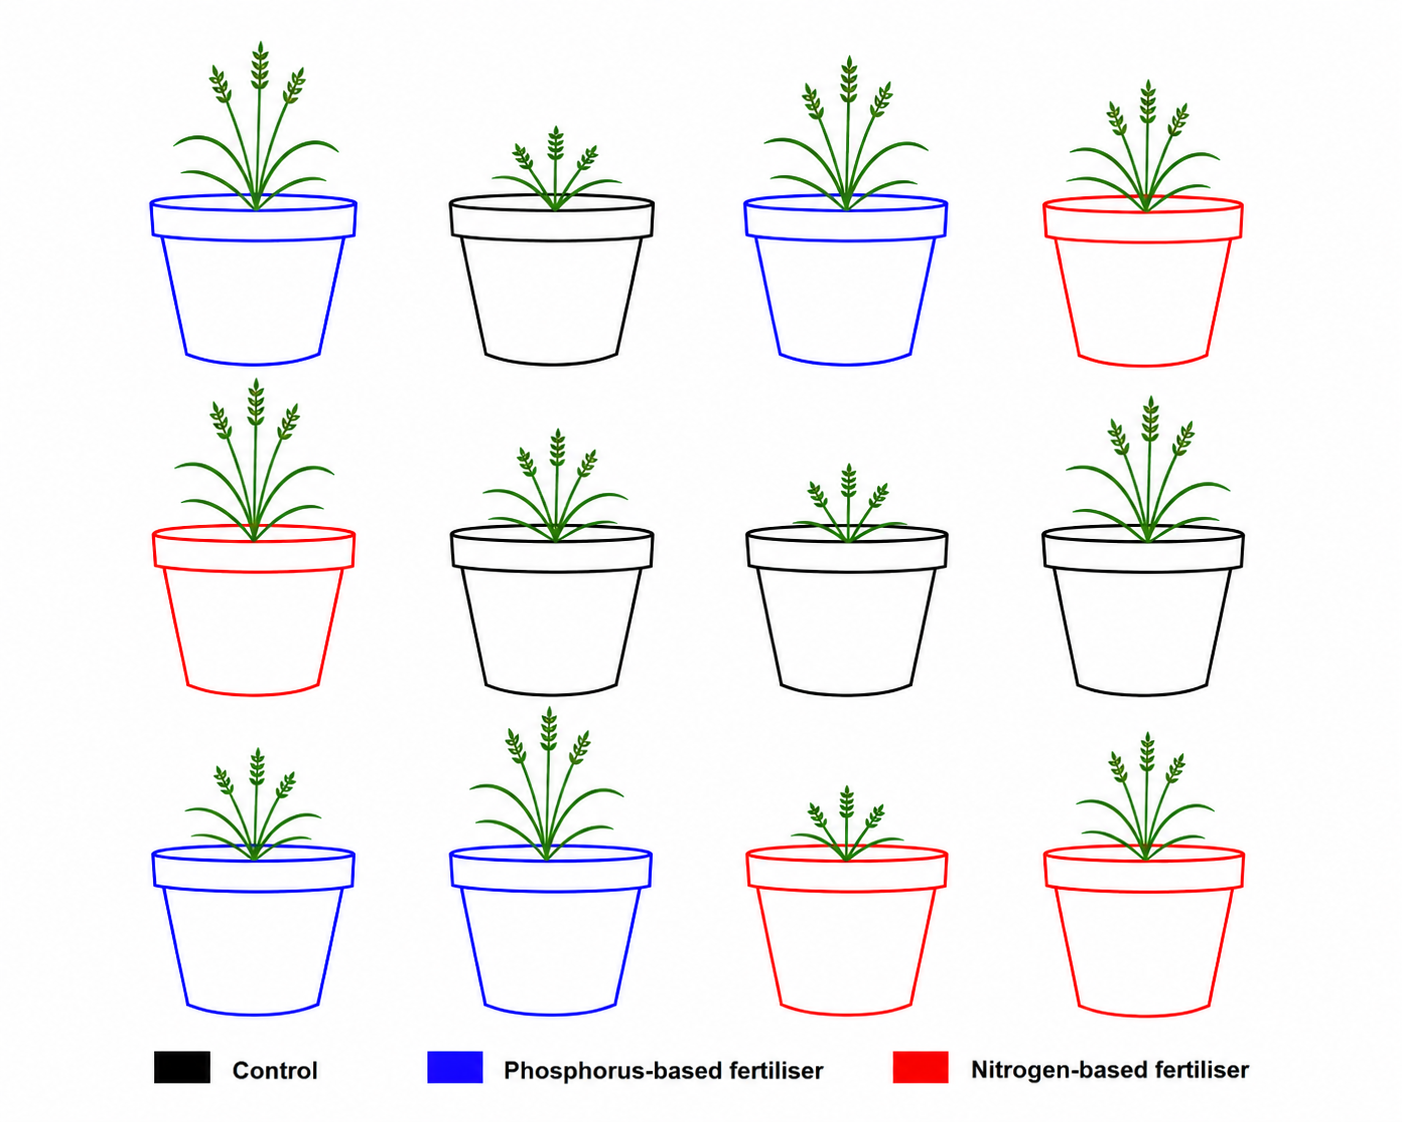
\includegraphics{img/fig1.png}

}

\caption{Figure 1. Fertiliser experiment}

\end{figure}%

Your starting assumption is that \emph{there is no difference in mean
plant height among the three groups.} The alternative is that at least
one fertiliser produces a different mean height.

Now consider the height of any single plant. Why does it differ from the
average height of all 12 plants (we will call this average height the
grand mean) ? There are two reasons.

\textbf{First}, that plant received a particular fertiliser, and that
fertiliser may genuinely promote or inhibit growth. This is what we will
call the \emph{treatment effect}. We use the term \emph{treatment}
because the fertilier is what was applied to the plant, and
\emph{effect} because it is the change in height that the fertiliser
brings about.

\textbf{Second}, even plants given the same fertiliser will not grow
identically. Tiny differences like seed quality, pot position, light
exposure, and watering can make each plant slightly different from its
neighbours. This uncontrollable scatter is what we will call
\emph{residual} or \emph{error}. We use the term \emph{residual} because
this second source of variation comes from all the factors that
influence plant height but are not measurd in the experiment, they are
leftover, the part of the story that the treament alone cannot tell.

The height of any single plant is therefore:

\[\text{Plant height} = \text{fertiliser effect} + \text{residual}\]

Suppose that we obtain the data below from the experiment:

\begin{longtable}[]{@{}ll@{}}
\toprule\noalign{}
Treatment & Plant height (cm) \\
\midrule\noalign{}
\endhead
\bottomrule\noalign{}
\endlastfoot
Control & 4 \\
Control & 5 \\
Control & 2 \\
Control & 1 \\
Nitrogen & 10 \\
Nitrogen & 8 \\
Nitrogen & 11 \\
Nitrogen & 7 \\
Phosphorus & 8 \\
Phosphorus & 4 \\
Phosphorus & 7 \\
Phosphorus & 5 \\
\end{longtable}

We have three groups of treatments: Control, Nitrogen, and Phosphorus.
Each treatment was \emph{randomly} assigned to a plant.

\subsection{The Grand Mean and Group
Means}\label{the-grand-mean-and-group-means}

Let us start with the bigger picture. By computing the mean of all 12
plant heights we obtain the \textbf{grand mean}:

\[\bar{x} = \frac{1}{n}\sum_{i=1}^{n} x_i
          = \frac{1}{12}(4 + 5 + 2 + 1 + 10 + 8 + 11 + 7 + 8 + 4 + 7 + 5)
          = 6 \text{ cm}\]

Computing the mean within each treatment group gives:

\[\bar{x}_{\text{control}} = \frac{1}{4}(4 + 5 + 2 + 1) = 3 \text{ cm}\]

\[\bar{x}_{\text{nitrogen}} = \frac{1}{4}(10 + 8 + 11 + 7) = 9 \text{ cm}\]

\[\bar{x}_{\text{phosphorus}} = \frac{1}{4}(8 + 4 + 7 + 5) = 6 \text{ cm}\]

Each group mean carries the effect of its treatment, but also the
influence of any unmeasured factor like differences in seed quality,
sunlight, watering, and so on. The nitrogen group mean of 9 cm, for
example, reflects both the genuine effect of nitrogen fertiliser on
growth \emph{and} the small random differences that existed between
those four plants regardless of what fertiliser they received.

\subsection{Among-Group Variation: The
Signal}\label{among-group-variation-the-signal}

If we compare each group mean to the grand mean, the control sits 3 cm
\emph{below} the grand mean, nitrogen sits 3 cm \emph{above} it, and
phosphorus sits right on it. Any displacement of a group mean from the
grand mean can come from two sources: the effect of the treatment, and
random error. If fertiliser has no effect whatsoever, the three group
means will cluster close to the grand mean, displaced only by chance. If
fertiliser genuinely matters, some means will be pulled far from the
grand mean, and the spread among group means will be large. This spread
is what we call \textbf{among-group variation}, and it is our window
onto the treatment effect.

\subsection{Within-Group Variation: The Noise}\label{sec-within-group}

Now look inside each group. Even though all four plants in the control
group received exactly the same treatment, no fertiliser at all, their
heights (4, 5, 2, 1 cm) are not identical. This scatter cannot come from
the fertiliser, since all four plants received the same one. It can only
reflect the residual, the unmeasured sources of variation we discussed
earlier. We can quantify this scatter with the within-group variance.
For the control group:

\[s^2_{\text{control}}
  = \frac{1}{n-1}\sum_{i=1}^{n}(x_i - \bar{x}_{\text{control}})^2
  = \frac{(4-3)^2 + (5-3)^2 + (2-3)^2 + (1-3)^2}{3}
  = \frac{1 + 4 + 1 + 4}{3}
  = 3.33 \text{ cm}^2\]

This within-group scatter, present in every group regardless of which
fertiliser was applied, is our estimate of background noise i.e.~the
residual variation the experiment cannot control. This is what we call
\textbf{within-group variation}.

\subsection{\texorpdfstring{The \(F\)
Ratio}{The F Ratio}}\label{the-f-ratio}

We now have two variance estimates that tell very different stories: the
among-group variance, which reflects the treatment effect plus noise,
and the within-group variance, which reflects noise alone. The natural
thing to do is form their ratio:

\[F = \frac{\text{Among-group variance (fertiliser + residual)}}
          {\text{Within-group variance (residual only)}}\]

When fertiliser has no effect, both the numerator and the denominator
are estimating the same background noise, and their ratio will hover
around 1. As the true differences among fertilisers grow larger, the
numerator grows, because the group means are being pulled further apart
by the treatment, while the denominator stays anchored to the background
noise. The ratio therefore climbs above 1, and the larger it becomes,
the harder it is to believe that the differences among groups arose by
chance alone.

\subsection{\texorpdfstring{Assessing the \(F\) Ratio: Is It Large
Enough?}{Assessing the F Ratio: Is It Large Enough?}}\label{assessing-the-f-ratio-is-it-large-enough}

Knowing that \(F\) is greater than 1 is not enough on its own, we need
to know how much greater than 1 it would have to be before we can
confidently say the differences are real. This is where probability
comes in.

When there is truly no treatment effect, the \(F\) ratio still varies
from experiment to experiment simply due to chance. Mathematical
statistics tells us that, under this condition, \(F\) follows a known
probability distribution called the \textbf{Fisher distribution} (or
\(F\)-distribution), whose shape depends on the degrees of freedom of
the two variance estimates. This distribution acts as a reference: it
tells us exactly how large \(F\) would typically be if there were no
fertiliser effect at all.

In practice, we choose a threshold probability in advance,
conventionally \(\alpha = 0.05\), which defines a critical value of
\(F\). If our observed \(F\) exceeds this critical value, it means that
the probability of seeing a ratio this large by chance alone is less
than 5\%. We then conclude that the differences among fertiliser groups
are unlikely to be due to chance.

If our observed \(F\) does not reach the critical value, we do not have
sufficient evidence to rule out chance as an explanation.

This is the core logic of the ANOVA test, and as we will see in the next
section, it is also the core logic of a much broader family of
statistical models.

\section{A Brief History of ANOVA}\label{a-brief-history-of-anova}

\subsection{Origins in Agriculture}\label{origins-in-agriculture}

The analysis of variance was developed in the early twentieth century by
the British statistician and geneticist Ronald A. Fisher, widely
regarded as the founder of modern statistics. Fisher developed the
method during his time at the Rothamsted Experimental Station in
Hertfordshire, England, where he worked from 1919 to 1933
\citep{fisher1919xv}. Rothamsted was, and remains, one of the oldest
agricultural research institutions in the world, and it was here that
Fisher was confronted with a practical problem: how to make sense of
large volumes of messy experimental data on crop yields, soil
treatments, and fertiliser effects.

The core challenge was not merely computational but conceptual.
Agricultural field experiments are inherently noisy. Soil fertility
varies across a field, weather is unpredictable, and individual plants
differ in ways that cannot be controlled. Fisher needed a principled way
to separate the variation caused by experimental treatments, different
fertilisers, crop varieties, tillage methods, from the background
variation that existed regardless of what the experimenter did. His
solution was the decomposition of total variance into distinct,
interpretable components: a idea that became the conceptual backbone of
ANOVA \citep{fisher1970statistical}.

\subsection{The Key Publications}\label{the-key-publications}

Fisher first introduced the F statistic and the logic of variance
decomposition in his landmark 1925 textbook \emph{Statistical Methods
for Research Workers} \citep{fisher1970statistical}. This work presented
ANOVA not as an abstract mathematical construction but as a practical
tool for scientists, illustrated throughout with agricultural and
biological examples. The book went through fourteen editions over
Fisher's lifetime and was enormously influential in spreading
statistical thinking across the life sciences.

Fisher elaborated the theory further in \emph{The Design of
Experiments}, published in 1935 \citep{fisher1935design}. This second
major work introduced the principles of randomisation, replication, and
blocking that underpin valid experimental design to this day, and showed
how ANOVA was inseparable from the way an experiment should be planned.
The famous example of the lady tasting tea, introduced in this book,
illustrated the logic of hypothesis testing in a way that remains a
staple of introductory statistics courses.

\subsection{\texorpdfstring{The \(F\)
Statistic}{The F Statistic}}\label{the-f-statistic}

The ratio of variances that lies at the heart of ANOVA, what we now call
the \(F\) statistic, was named in Fisher's honour by George W. Snedecor,
the American statistician who popularised and extended Fisher's methods
in the United States \citep{snedecor1934}. Snedecor introduced the
notation \(F\) explicitly as a tribute, and the name has remained
standard ever since.

\subsection{From Agriculture to All of
Science}\label{from-agriculture-to-all-of-science}

Although ANOVA was born from the needs of agricultural research, its
logic proved universal. By the mid-twentieth century it had been adopted
across medicine, psychology, ecology, and engineering, wherever
researchers needed to compare means across multiple groups while
accounting for background noise. Today it remains one of the most widely
used statistical procedures in empirical science
\citep{montgomery2017design}.

The enduring power of ANOVA lies precisely in the simplicity of the idea
Fisher identified at Rothamsted: that variation is not an obstacle to
understanding, but a quantity that can be measured, partitioned, and
interpreted.

\section{ANOVA as a special case of linear
models}\label{anova-as-a-special-case-of-linear-models}

\subsection{The linear model idea}\label{the-linear-model-idea}

You may have already encountered simple linear regression: the idea that
you can predict one variable from another using a straight line. For
example, you might predict plant height from the amount of rainfall
received. The equation looks like this:

\[\text{Plant height} = \beta_0 + \beta_1 \times \text{Rainfall} + \varepsilon\]

where \(\beta_0\) is the intercept (the expected height when rainfall is
zero), \(\beta_1\) is the slope (how much height changes for each
additional unit of rainfall), and \(\varepsilon\) is the error, the
residual scatter around the line that rainfall alone cannot explain.

This is called a \textbf{linear model}: we are modelling the response
variable (plant height) as a linear combination of some predictor plus
error.

\textbf{ANOVA is in fact the same thing}. The only difference is that
instead of a continuous predictor like rainfall, \emph{our predictor is
a categorical variable}, a group label like \emph{control},
\emph{nitrogen}, or \emph{phosphorus}.

\subsection{Recoding groups as numbers: dummy
variables}\label{recoding-groups-as-numbers-dummy-variables}

A computer cannot do arithmetic on the words ``control'' or
``nitrogen'', so we recode the group labels as numbers. This is done
using \textbf{dummy variables} (also called indicator variables). The
idea is simple: we pick one group as the reference, say, the control,
and then create one dummy variable for each of the other groups.

For our fertiliser experiment with \textbf{three groups}, we create
\textbf{two dummy variables}:

\[X_1 = \begin{cases} 1 & \text{if the plant received nitrogen} \\ 
0 & \text{otherwise} \end{cases}\]

\[X_2 = \begin{cases} 1 & \text{if the plant received phosphorus} \\ 
0 & \text{otherwise} \end{cases}\]

Notice that a control plant gets \(X_1 = 0\) and \(X_2 = 0\): it is
identified by the absence of both flags. \textbf{We never need a third
dummy variable for the control group because it is already fully
described this way.}

The table below shows how the 12 plants in our experiment are recoded:

\begin{longtable}[]{@{}llcc@{}}
\toprule\noalign{}
Plant & Group & \(X_1\) (nitrogen) & \(X_2\) (phosphorus) \\
\midrule\noalign{}
\endhead
\bottomrule\noalign{}
\endlastfoot
1 & Control & 0 & 0 \\
2 & Control & 0 & 0 \\
3 & Control & 0 & 0 \\
4 & Control & 0 & 0 \\
5 & Nitrogen & 1 & 0 \\
6 & Nitrogen & 1 & 0 \\
7 & Nitrogen & 1 & 0 \\
8 & Nitrogen & 1 & 0 \\
9 & Phosphorus & 0 & 1 \\
10 & Phosphorus & 0 & 1 \\
11 & Phosphorus & 0 & 1 \\
12 & Phosphorus & 0 & 1 \\
\end{longtable}

Notice the pattern: each group has its own ``signature'' of zeros and
ones. The control group is the only group with zeros in \emph{both}
columns, which is why it serves naturally as the reference against which
the other groups are compared.

\subsection{Writing the model}\label{writing-the-model}

We can now write the ANOVA as a linear model:

\[\text{Plant height} = \beta_0 + \beta_1 X_1 + \beta_2 X_2 + \varepsilon\]

The coefficients have a beautifully simple interpretation:

\begin{itemize}
\tightlist
\item
  \(\beta_0\) is the mean height of the \textbf{control} group (when
  \(X_1 = 0\) and \(X_2 = 0\)).
\item
  \(\beta_1\) is the \textbf{difference} in mean height between the
  nitrogen group and the control group.
\item
  \(\beta_2\) is the \textbf{difference} in mean height between the
  phosphorus group and the control group.
\item
  \(\varepsilon\) is the residual error for each individual plant.
\end{itemize}

Let us check this with a concrete example. Suppose the estimated
coefficients are:

\[\hat{\beta}_0 = 20 \text{ cm}, \quad \hat{\beta}_1 = 5 \text{ cm}, 
\quad \hat{\beta}_2 = 2 \text{ cm}\]

Then the model predicts:

\begin{itemize}
\tightlist
\item
  A \textbf{control} plant: \(20 + 5 \times 0 + 2 \times 0 = 20\) cm
\item
  A \textbf{nitrogen} plant: \(20 + 5 \times 1 + 2 \times 0 = 25\) cm
\item
  A \textbf{phosphorus} plant: \(20 + 5 \times 0 + 2 \times 1 = 22\) cm
\end{itemize}

In other words, nitrogen fertiliser is associated with plants that are
on average 5 cm taller than the control, and phosphorus with plants that
are 2 cm taller.

\subsection{\texorpdfstring{The connection to the \(F\)
test}{The connection to the F test}}\label{the-connection-to-the-f-test}

In the linear model framework, the null hypothesis of ANOVA, \emph{no
difference in mean height among groups}, translates directly into:

\[H_0: \beta_1 = 0 \quad \text{and} \quad \beta_2 = 0\]

That is, we are testing whether all the group coefficients are
simultaneously zero. If they are, then the group labels carry no
information and the model reduces to:

\[\text{Plant height} = \beta_0 + \varepsilon\]

which simply says every plant has the same expected height (the grand
mean) plus noise. \textbf{The \(F\) test in ANOVA is exactly the test of
this hypothesis: it compares how much better the full model (with group
labels) fits the data compared to this reduced model (with no group
labels).} A large \(F\) means the group labels explain a meaningful
amount of the variation in height, and we reject \(H_0\).

\subsection{Why Does This Matter?}\label{why-does-this-matter}

Recognising ANOVA as a linear model is more than a mathematical
curiosity. It means that \textbf{ANOVA and regression are not two
separate tools you need to learn independently, they are both special
cases of a single unified framework, the general linear model}. Once you
are comfortable with this framework, you can naturally extend your
analyses to situations that mix categorical and continuous predictors
(called ANCOVA), include multiple categorical factors (two-way ANOVA),
or handle more complex experimental designs, all within exactly the same
logic you have already learned here.

\section{\texorpdfstring{What ANOVA is \textbf{not}: common
misconceptions}{What ANOVA is not: common misconceptions}}\label{what-anova-is-not-common-misconceptions}

\subsection{ANOVA Does Not Tell You Which Groups
Differ}\label{anova-does-not-tell-you-which-groups-differ}

This is perhaps the most common source of confusion among newcomers. A
significant \(F\) test tells you that the group means are not all equal
i.e that somewhere among your groups there is a real difference. It does
not tell you \emph{where} that difference lies.

In our fertiliser example, a significant result tells you that
fertiliser type matters, but it does not tell you whether nitrogen
differs from the control, whether phosphorus differs from the control,
or whether nitrogen and phosphorus differ from each other. Identifying
which specific pairs of groups differ requires additional
\textbf{post-hoc tests}, such as Tukey's HSD or pairwise \(t\)-tests
with corrected significance thresholds, which are conducted after the
ANOVA, and only when the \(F\) test is significant.

\subsection{A Non-Significant Result Does Not Mean the Groups Are
Equal}\label{a-non-significant-result-does-not-mean-the-groups-are-equal}

If your \(F\) test returns \(p > 0.05\), it is tempting to conclude that
the fertilisers have no effect on plant height. \textbf{This conclusion
is not warranted.} A non-significant result means only that \emph{you
did not find sufficient evidence of a difference given your data}. There
are many reasons this can happen even when a true difference exists:

\begin{itemize}
\tightlist
\item
  Your sample size may have been too small to detect a modest effect.
\item
  The within-group variation (error) may have been large, drowning out a
  real treatment signal.
\item
  The effect of the treatment may be genuine but smaller than your
  experiment was designed to detect.
\end{itemize}

\textbf{The absence of evidence is not evidence of absence.} A
non-significant ANOVA should prompt you to think about the
\textbf{statistical power} of your experiment: its ability to detect an
effect of a given size, rather than to simply accept the null
hypothesis.

\subsection{ANOVA Does Not Require Equal Sample Sizes, But Imbalance Has
Consequences}\label{anova-does-not-require-equal-sample-sizes-but-imbalance-has-consequences}

It is a common belief that ANOVA requires the same number of
observations in each group. This is not strictly true: ANOVA can be
performed on unbalanced designs where group sizes differ. However, equal
sample sizes are strongly preferred. Balanced designs are more
statistically efficient, more robust to violations of the assumption of
equal variances, and considerably simpler to interpret. If your groups
are very unequal in size, the results of the \(F\) test can become
sensitive to assumptions you might not have checked carefully.

\subsection{ANOVA is not robust to all assumption
violations}\label{anova-is-not-robust-to-all-assumption-violations}

ANOVA rests on three key assumptions:

\begin{enumerate}
\def\labelenumi{\arabic{enumi}.}
\tightlist
\item
  \textbf{Independence}: the observations are independent of one
  another.
\item
  \textbf{Normality}: the residuals (errors) are approximately normally
  distributed within each group.
\item
  \textbf{Homogeneity of variance}: the variance within each group is
  approximately the same (also called homoscedasticity).
\end{enumerate}

Students sometimes assume that ANOVA is so widely used that it must be
safe to apply in any situation. This is not the case. Of the three
assumptions above, independence is by far the most critical. Violating
it, for example by measuring the same plant twice and treating the two
measurements as independent observations, can severely inflate your
false positive rate and lead to entirely spurious conclusions.
Violations of normality are generally less serious, especially with
larger sample sizes, thanks to the central limit theorem. Violations of
homogeneity of variance are intermediate in severity and can be
addressed with modified versions of the test, such as Welch's ANOVA.

We will explore the assumptions of ANOVA in the following chapter.

\subsection{ANOVA is not a test of means
alone}\label{anova-is-not-a-test-of-means-alone}

Although ANOVA is typically introduced as a way to compare means, what
it actually does is partition and compare \emph{variances}. The \(F\)
ratio is a ratio of two variance estimates, not a direct comparison of
means. The connection to means is real, a large among-group variance
arises precisely because the group means are far apart, but it is
important to understand that ANOVA is fundamentally a test about the
structure of variation in your data. This is why, as we saw in the
previous section, ANOVA fits so naturally within the linear model
framework: both are concerned with explaining variation, not merely
comparing averages.

\subsection{ANOVA is not a substitute for good experimental
design}\label{anova-is-not-a-substitute-for-good-experimental-design}

Finally, and perhaps most importantly, no statistical test can rescue a
poorly designed experiment. ANOVA assumes that your groups were formed
by proper randomisation, that your replicates are genuine independent
observations, and that sources of systematic bias have been controlled
or accounted for. If your four control plants were all placed on one
side of the greenhouse and your four nitrogen plants on the other, then
any difference you observe might reflect a light or temperature gradient
rather than a fertiliser effect. ANOVA will dutifully compute an \(F\)
statistic and a \(p\)-value in this situation, but the result will be
meaningless. As Fisher himself understood from his years at Rothamsted,
the validity of the analysis begins not at the computer but at the
moment the experiment is designed.

\chapter{The Assumptions}\label{sec-chap2}

\section{Independence of observations}\label{sec-independence}

\subsection{What does independence
mean?}\label{what-does-independence-mean}

Of all the assumptions underlying ANOVA, independence is the most
important and, paradoxically, the least discussed in introductory
courses. \textbf{The assumption states that knowing the value of one
observation tells you nothing about the value of any other observation.}
Each data point must carry its own independent piece of information.

This sounds abstract, so let us ground it in a concrete example.

Imagine you are measuring the effect of three diets on the weight gain
of mice. You have 12 mice, four per diet group. If each mouse lives in
its own individual cage, eats its own food, and is weighed
independently. Then the 12 measurements are independent: the weight of
one mouse gives you no information about the weight of any other.

Now imagine instead that you house all four mice in each diet group
together in a single shared cage. The mice in the same cage eat
together, sleep together, and influence each other's behaviour. A
dominant mouse may monopolise food; a stressed mouse may eat less. The
four measurements within each cage are no longer independent: they are
\textbf{clustered}. Knowing that one mouse in a cage gained a lot of
weight makes it more likely that its cagemates did too, simply because
they share the same environment.

This is the essence of non-independence: observations that are
\textbf{grouped, nested, repeated, or spatially clustered} tend to
resemble each other more than random chance would predict.

\subsection{Why does it matter so
much?}\label{why-does-it-matter-so-much}

ANOVA and the \(F\) test in particular, is built on the assumption that
the within-group variance faithfully estimates background noise. When
observations are not independent, this estimate is distorted.
Specifically, clustered observations tend to be more similar to each
other than truly independent observations would be, which
\textbf{artificially deflates the within-group variance}. A smaller
denominator in the \(F\) ratio means a larger \(F\) statistic, and
therefore a smaller \(p\)-value, even when there is no real treatment
effect. \textbf{In other words, non-independence makes you think you
have found something when you have not.}

This inflation of the false positive rate is not a minor inconvenience.
It can be dramatic, as the simulation below will demonstrate.

\subsection{A concrete example:
pseudoreplication}\label{sec-pseudoreplication}

The most common form of non-independence in biology is
\textbf{pseudoreplication}: the mistake of treating non-independent
measurements as if they were independent replicates
\citep{hurlbert1984}.

Returning to our mice: suppose you have three diet groups, each with two
cages, and two mice per cage, 12 mice in total. The true replicates are
the \textbf{cages} (since each cage is an independent experimental
unit), not the individual mice. If you ignore the cage structure and run
ANOVA on the 12 individual mouse weights as if they were 12 independent
observations, you are pseudoreplicating. Your apparent \(n = 12\) is an
illusion, you effectively have only \(n = 6\) independent units.

The following R code simulates this scenario.

\begin{Shaded}
\begin{Highlighting}[]
\FunctionTok{set.seed}\NormalTok{(}\DecValTok{42}\NormalTok{)}

\NormalTok{n\_sim }\OtherTok{\textless{}{-}} \DecValTok{5000}  \CommentTok{\# number of simulations}
\NormalTok{alpha }\OtherTok{\textless{}{-}} \FloatTok{0.05}  \CommentTok{\# significance threshold}
\NormalTok{n\_diets }\OtherTok{\textless{}{-}} \DecValTok{3}   \CommentTok{\# number of diet groups}
\NormalTok{n\_cages }\OtherTok{\textless{}{-}} \DecValTok{2}   \CommentTok{\# cages per diet group}
\NormalTok{n\_mice }\OtherTok{\textless{}{-}} \DecValTok{2}    \CommentTok{\# mice per cage}
\NormalTok{cage\_sd }\OtherTok{\textless{}{-}} \DecValTok{2}   \CommentTok{\# variation among cages (shared environment effect)}
\NormalTok{mouse\_sd }\OtherTok{\textless{}{-}} \DecValTok{1}  \CommentTok{\# variation among mice within a cage}

\NormalTok{false\_pos\_correct }\OtherTok{\textless{}{-}} \FunctionTok{logical}\NormalTok{(n\_sim)}
\NormalTok{false\_pos\_pseudo }\OtherTok{\textless{}{-}} \FunctionTok{logical}\NormalTok{(n\_sim)}

\ControlFlowTok{for}\NormalTok{ (i }\ControlFlowTok{in} \FunctionTok{seq\_len}\NormalTok{(n\_sim)) \{}
  
  \CommentTok{\# Build the data structure}
\NormalTok{  diet }\OtherTok{\textless{}{-}} \FunctionTok{rep}\NormalTok{(}\FunctionTok{paste0}\NormalTok{(}\StringTok{"Diet"}\NormalTok{, }\DecValTok{1}\SpecialCharTok{:}\NormalTok{n\_diets), }\AttributeTok{each =}\NormalTok{ n\_cages }\SpecialCharTok{*}\NormalTok{ n\_mice)}
\NormalTok{  cage }\OtherTok{\textless{}{-}} \FunctionTok{rep}\NormalTok{(}\FunctionTok{paste0}\NormalTok{(}\StringTok{"Cage"}\NormalTok{, }\DecValTok{1}\SpecialCharTok{:}\NormalTok{(n\_diets }\SpecialCharTok{*}\NormalTok{ n\_cages)), }\AttributeTok{each =}\NormalTok{ n\_mice)}
  
  \CommentTok{\# Cage{-}level random effect (shared environment, no diet effect)}
\NormalTok{  cage\_effect }\OtherTok{\textless{}{-}} \FunctionTok{rep}\NormalTok{(}\FunctionTok{rnorm}\NormalTok{(n\_diets }\SpecialCharTok{*}\NormalTok{ n\_cages, }\AttributeTok{mean =} \DecValTok{0}\NormalTok{, }\AttributeTok{sd =}\NormalTok{ cage\_sd), }\AttributeTok{each =}\NormalTok{ n\_mice)}
  
  \CommentTok{\# Individual mouse noise}
\NormalTok{  mouse\_noise }\OtherTok{\textless{}{-}} \FunctionTok{rnorm}\NormalTok{(n\_diets }\SpecialCharTok{*}\NormalTok{ n\_cages }\SpecialCharTok{*}\NormalTok{ n\_mice, }\AttributeTok{mean =} \DecValTok{0}\NormalTok{, }\AttributeTok{sd =}\NormalTok{ mouse\_sd)}
  
  \CommentTok{\# Response: no diet effect, only cage effect + individual noise}
\NormalTok{  weight\_gain }\OtherTok{\textless{}{-}} \DecValTok{10} \SpecialCharTok{+}\NormalTok{ cage\_effect }\SpecialCharTok{+}\NormalTok{ mouse\_noise}
  
\NormalTok{  df }\OtherTok{\textless{}{-}} \FunctionTok{data.frame}\NormalTok{(diet, cage, weight\_gain)}
  
  \CommentTok{\# {-}{-}{-} Correct analysis: use cage means {-}{-}{-}}
\NormalTok{  cage\_means }\OtherTok{\textless{}{-}} \FunctionTok{aggregate}\NormalTok{(weight\_gain }\SpecialCharTok{\textasciitilde{}}\NormalTok{ diet }\SpecialCharTok{+}\NormalTok{ cage, }\AttributeTok{data =}\NormalTok{ df, }\AttributeTok{FUN =}\NormalTok{ mean)}
\NormalTok{  fit\_correct }\OtherTok{\textless{}{-}} \FunctionTok{aov}\NormalTok{(weight\_gain }\SpecialCharTok{\textasciitilde{}}\NormalTok{ diet, }\AttributeTok{data =}\NormalTok{ cage\_means)}
\NormalTok{  p\_correct   }\OtherTok{\textless{}{-}} \FunctionTok{summary}\NormalTok{(fit\_correct)[[}\DecValTok{1}\NormalTok{]][[}\StringTok{"Pr(\textgreater{}F)"}\NormalTok{]][}\DecValTok{1}\NormalTok{]}
\NormalTok{  false\_pos\_correct[i] }\OtherTok{\textless{}{-}}\NormalTok{ p\_correct }\SpecialCharTok{\textless{}}\NormalTok{ alpha}
  
  \CommentTok{\# {-}{-}{-} Incorrect analysis: ignore cage structure (pseudoreplication) {-}{-}{-}}
\NormalTok{  fit\_pseudo }\OtherTok{\textless{}{-}} \FunctionTok{aov}\NormalTok{(weight\_gain }\SpecialCharTok{\textasciitilde{}}\NormalTok{ diet, }\AttributeTok{data =}\NormalTok{ df)}
\NormalTok{  p\_pseudo   }\OtherTok{\textless{}{-}} \FunctionTok{summary}\NormalTok{(fit\_pseudo)[[}\DecValTok{1}\NormalTok{]][[}\StringTok{"Pr(\textgreater{}F)"}\NormalTok{]][}\DecValTok{1}\NormalTok{]}
\NormalTok{  false\_pos\_pseudo[i] }\OtherTok{\textless{}{-}}\NormalTok{ p\_pseudo }\SpecialCharTok{\textless{}}\NormalTok{ alpha}
  
\NormalTok{\}}
\end{Highlighting}
\end{Shaded}

Running this code produces output along the lines of:

\begin{Shaded}
\begin{Highlighting}[]
\FunctionTok{cat}\NormalTok{(}
  \StringTok{"False positive rate (correct analysis):"}\NormalTok{,}
  \FunctionTok{round}\NormalTok{(}\FunctionTok{mean}\NormalTok{(false\_pos\_correct), }\DecValTok{3}\NormalTok{),}
  \StringTok{"}\SpecialCharTok{\textbackslash{}n}\StringTok{False positive rate (pseudoreplication):"}\NormalTok{,}
  \FunctionTok{round}\NormalTok{(}\FunctionTok{mean}\NormalTok{(false\_pos\_pseudo), }\DecValTok{3}\NormalTok{), }\StringTok{"}\SpecialCharTok{\textbackslash{}n}\StringTok{"}
\NormalTok{  )}
\end{Highlighting}
\end{Shaded}

\begin{verbatim}
#> False positive rate (correct analysis): 0.053 
#> False positive rate (pseudoreplication): 0.27
\end{verbatim}

The correct analysis produces a false positive rate right at the nominal
5\% level: exactly as it should when there is no real effect. The
pseudoreplicated analysis produces a false positive rate of around
\textbf{27 \%}: more than one in four experiments would be declared
significant by chance alone, simply because the cage structure was
ignored.

We can visualise the distribution of \(p\)-values from both approaches
across the 5000 simulations.

First we simulate the distributions.

\begin{Shaded}
\begin{Highlighting}[]
\FunctionTok{set.seed}\NormalTok{(}\DecValTok{42}\NormalTok{)}

\NormalTok{n\_sim }\OtherTok{\textless{}{-}} \DecValTok{5000}
\NormalTok{alpha }\OtherTok{\textless{}{-}} \FloatTok{0.05}
\NormalTok{n\_diets }\OtherTok{\textless{}{-}} \DecValTok{3}
\NormalTok{n\_cages }\OtherTok{\textless{}{-}} \DecValTok{2}
\NormalTok{n\_mice }\OtherTok{\textless{}{-}} \DecValTok{2}
\NormalTok{cage\_sd }\OtherTok{\textless{}{-}} \DecValTok{2}
\NormalTok{mouse\_sd }\OtherTok{\textless{}{-}} \DecValTok{1}

\NormalTok{p\_correct }\OtherTok{\textless{}{-}} \FunctionTok{numeric}\NormalTok{(n\_sim)}
\NormalTok{p\_pseudo }\OtherTok{\textless{}{-}} \FunctionTok{numeric}\NormalTok{(n\_sim)}

\ControlFlowTok{for}\NormalTok{ (i }\ControlFlowTok{in} \FunctionTok{seq\_len}\NormalTok{(n\_sim)) \{}
\NormalTok{  diet }\OtherTok{\textless{}{-}} \FunctionTok{rep}\NormalTok{(}\FunctionTok{paste0}\NormalTok{(}\StringTok{"Diet"}\NormalTok{, }\DecValTok{1}\SpecialCharTok{:}\NormalTok{n\_diets), }\AttributeTok{each =}\NormalTok{ n\_cages }\SpecialCharTok{*}\NormalTok{ n\_mice)}
\NormalTok{  cage }\OtherTok{\textless{}{-}} \FunctionTok{rep}\NormalTok{(}\FunctionTok{paste0}\NormalTok{(}\StringTok{"Cage"}\NormalTok{, }\DecValTok{1}\SpecialCharTok{:}\NormalTok{(n\_diets }\SpecialCharTok{*}\NormalTok{ n\_cages)), }\AttributeTok{each =}\NormalTok{ n\_mice)}
  
\NormalTok{  cage\_effect }\OtherTok{\textless{}{-}} \FunctionTok{rep}\NormalTok{(}
    \FunctionTok{rnorm}\NormalTok{(n\_diets }\SpecialCharTok{*}\NormalTok{ n\_cages, }\AttributeTok{mean =} \DecValTok{0}\NormalTok{, }\AttributeTok{sd =}\NormalTok{ cage\_sd),}
    \AttributeTok{each =}\NormalTok{ n\_mice}
\NormalTok{  )}
\NormalTok{  mouse\_noise }\OtherTok{\textless{}{-}} \FunctionTok{rnorm}\NormalTok{(n\_diets }\SpecialCharTok{*}\NormalTok{ n\_cages }\SpecialCharTok{*}\NormalTok{ n\_mice, }\AttributeTok{mean =} \DecValTok{0}\NormalTok{, }\AttributeTok{sd =}\NormalTok{ mouse\_sd)}
  
\NormalTok{  weight\_gain }\OtherTok{\textless{}{-}} \DecValTok{10} \SpecialCharTok{+}\NormalTok{ cage\_effect }\SpecialCharTok{+}\NormalTok{ mouse\_noise}
  
\NormalTok{  df }\OtherTok{\textless{}{-}} \FunctionTok{data.frame}\NormalTok{(diet, cage, weight\_gain)}
  
  \CommentTok{\# Correct analysis: cage means as the unit of analysis}
\NormalTok{  cage\_means  }\OtherTok{\textless{}{-}} \FunctionTok{aggregate}\NormalTok{(weight\_gain }\SpecialCharTok{\textasciitilde{}}\NormalTok{ diet }\SpecialCharTok{+}\NormalTok{ cage, }\AttributeTok{data =}\NormalTok{ df, }\AttributeTok{FUN =}\NormalTok{ mean)}
\NormalTok{  p\_correct[i] }\OtherTok{\textless{}{-}} \FunctionTok{summary}\NormalTok{(}
    \FunctionTok{aov}\NormalTok{(weight\_gain }\SpecialCharTok{\textasciitilde{}}\NormalTok{ diet, }\AttributeTok{data =}\NormalTok{ cage\_means)}
\NormalTok{    )[[}\DecValTok{1}\NormalTok{]][[}\StringTok{"Pr(\textgreater{}F)"}\NormalTok{]][}\DecValTok{1}\NormalTok{]}
  
  \CommentTok{\# Incorrect analysis: pseudoreplication}
\NormalTok{  p\_pseudo[i]  }\OtherTok{\textless{}{-}} \FunctionTok{summary}\NormalTok{(}
    \FunctionTok{aov}\NormalTok{(weight\_gain }\SpecialCharTok{\textasciitilde{}}\NormalTok{ diet, }\AttributeTok{data =}\NormalTok{ df)}
\NormalTok{    )[[}\DecValTok{1}\NormalTok{]][[}\StringTok{"Pr(\textgreater{}F)"}\NormalTok{]][}\DecValTok{1}\NormalTok{]}
\NormalTok{\}}
\end{Highlighting}
\end{Shaded}

Then, we can check the false positive rate:

\begin{Shaded}
\begin{Highlighting}[]
\FunctionTok{cat}\NormalTok{(}
  \StringTok{"False positive rate (correct analysis):"}\NormalTok{,}
  \FunctionTok{round}\NormalTok{(}\FunctionTok{mean}\NormalTok{(p\_correct }\SpecialCharTok{\textless{}}\NormalTok{ alpha), }\DecValTok{3}\NormalTok{),}
  \StringTok{"}\SpecialCharTok{\textbackslash{}n}\StringTok{False positive rate (pseudoreplication):"}\NormalTok{,}
  \FunctionTok{round}\NormalTok{(}\FunctionTok{mean}\NormalTok{(p\_pseudo  }\SpecialCharTok{\textless{}}\NormalTok{ alpha), }\DecValTok{3}\NormalTok{), }\StringTok{"}\SpecialCharTok{\textbackslash{}n}\StringTok{"}
\NormalTok{  )}
\end{Highlighting}
\end{Shaded}

\begin{verbatim}
#> False positive rate (correct analysis): 0.053 
#> False positive rate (pseudoreplication): 0.27
\end{verbatim}

And visualise the distribution of p-values:

\begin{Shaded}
\begin{Highlighting}[]
\FunctionTok{library}\NormalTok{(ggplot2)}

\CommentTok{\# Build a tidy data frame for plotting}
\NormalTok{p\_df }\OtherTok{\textless{}{-}} \FunctionTok{data.frame}\NormalTok{(}
  \AttributeTok{p\_value  =} \FunctionTok{c}\NormalTok{(p\_correct, p\_pseudo),}
  \AttributeTok{analysis =} \FunctionTok{rep}\NormalTok{(}\FunctionTok{c}\NormalTok{(}\StringTok{"Correct (cage means)"}\NormalTok{, }\StringTok{"Pseudoreplication"}\NormalTok{), }\AttributeTok{each =}\NormalTok{ n\_sim)}
\NormalTok{)}
  
\FunctionTok{ggplot}\NormalTok{(p\_df, }\FunctionTok{aes}\NormalTok{(}\AttributeTok{x =}\NormalTok{ p\_value, }\AttributeTok{fill =}\NormalTok{ analysis)) }\SpecialCharTok{+}
  \FunctionTok{geom\_histogram}\NormalTok{(}\AttributeTok{binwidth =} \FloatTok{0.05}\NormalTok{, }\AttributeTok{boundary =} \DecValTok{0}\NormalTok{, }\AttributeTok{colour =} \StringTok{"white"}\NormalTok{) }\SpecialCharTok{+}
  \FunctionTok{facet\_wrap}\NormalTok{(}\SpecialCharTok{\textasciitilde{}}\NormalTok{ analysis, }\AttributeTok{ncol =} \DecValTok{1}\NormalTok{) }\SpecialCharTok{+}
  \FunctionTok{geom\_vline}\NormalTok{(}\AttributeTok{xintercept =} \FloatTok{0.05}\NormalTok{, }\AttributeTok{linetype =} \StringTok{"dashed"}\NormalTok{, }\AttributeTok{colour =} \StringTok{"red"}\NormalTok{) }\SpecialCharTok{+}
  \FunctionTok{scale\_fill\_manual}\NormalTok{(}\AttributeTok{values =} \FunctionTok{c}\NormalTok{(}\StringTok{"\#2E86AB"}\NormalTok{, }\StringTok{"\#E84855"}\NormalTok{)) }\SpecialCharTok{+}
  \FunctionTok{labs}\NormalTok{(}\AttributeTok{x =} \StringTok{"p{-}value"}\NormalTok{, }\AttributeTok{y =} \StringTok{"Count"}\NormalTok{, }\AttributeTok{fill =} \StringTok{"Analysis type"}\NormalTok{) }\SpecialCharTok{+}
  \FunctionTok{theme\_bw}\NormalTok{() }\SpecialCharTok{+}
  \FunctionTok{theme}\NormalTok{(}\AttributeTok{legend.position =} \StringTok{"none"}\NormalTok{)}
\end{Highlighting}
\end{Shaded}

\begin{figure}[H]

\centering{

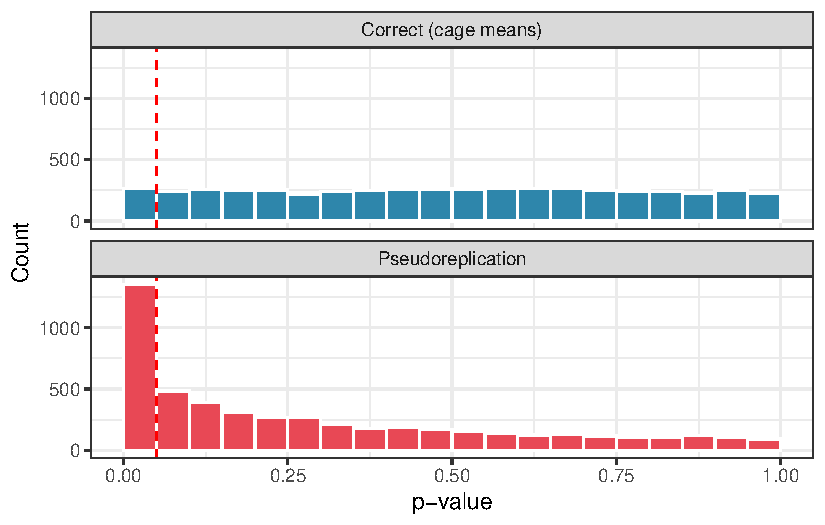
\includegraphics[width=0.9\textwidth,height=\textheight]{02b-assumptions_files/figure-pdf/fig-pval-1.pdf}

}

\caption{\label{fig-pval}Distribution of p-values under the null
hypothesis across 5000 simulations. Under the correct analysis (top),
p-values are uniformly spread between 0 and 1, the expected behaviour of
a well-calibrated test. Under pseudoreplication (bottom), p-values pile
up near zero, producing a large excess of spurious significant results.
Red dashed line marks p = 0.05.}

\end{figure}%

Under the correct analysis, \(p\)-values are uniformly distributed
between 0 and 1, the signature of a well-calibrated test under the null
hypothesis. Under pseudoreplication, \(p\)-values pile up near zero,
producing an excess of spurious significant results.

\subsection{How to detect
non-independence}\label{how-to-detect-non-independence}

Independence is not something you can test statistically after the fact:
it must be assessed by thinking carefully about \textbf{how the data
were collected}. Ask yourself: - Are any observations collected from the
same individual at different times? - Are any observations grouped
within a shared physical unit (a cage, a pot, a plot, a classroom, a
hospital ward)? - Could observations close together in space or time be
more similar to each other than observations far apart?

If the answer to any of these questions is yes, your observations are
likely not fully independent, and a standard ANOVA may not be
appropriate.

\subsection{What to do when independence is
violated}\label{what-to-do-when-independence-is-violated}

The good news is that non-independence is not a dead end: \textbf{it is
a feature of your data that can be modelled explicitly}. The appropriate
tools depend on the structure of the dependence:

\begin{itemize}
\tightlist
\item
  \textbf{Repeated measures ANOVA} handles the case where the same
  individual is measured multiple times.
\item
  \textbf{Mixed-effects models} (also called multilevel or hierarchical
  models) handle nested structures such as mice within cages, students
  within classrooms, or plots within fields. These models estimate the
  cage-level (or cluster-level) variance explicitly rather than
  pretending it does not exist.
\end{itemize}

In all cases, the key principle is the same: \textbf{the unit of
replication in your statistical analysis must match the unit of
replication in your experimental design.} If the cage is the
experimental unit, the thing that received the treatment, then the cage,
not the individual mouse, must be the unit of analysis.

\section{Homogeneity of Variances
(Homoscedasticity)}\label{sec-homoscedasticity}

\subsection{What does the assumption
say?}\label{what-does-the-assumption-say}

ANOVA assumes that the variance of the residuals, the scatter of
individual observations around their group mean, is the same in every
group. This property is called \textbf{homoscedasticity}, from the Greek
for ``same scatter''. Its opposite, \textbf{heteroscedasticity}, refers
to situations where different groups have different amounts of internal
variation. Concretely, in our fertiliser experiment, homoscedasticity
means that the spread of plant heights around the control mean, the
spread around the nitrogen mean, and the spread around the phosphorus
mean should all be approximately equal. \textbf{The groups may differ in
their \emph{means}, that is what we are testing, but they should not
differ in their \emph{variances}.}

\subsection{Why does ANOVA need this?}\label{why-does-anova-need-this}

Recall that the \(F\) ratio is built on two variance estimates:

\[F = \frac{\text{Among-group variance}}{\text{Within-group variance}}\]

The within-group variance is computed by \textbf{pooling} the scatter
from all groups together into a single estimate of background noise.
This pooling is only legitimate if the groups genuinely share the same
underlying variance. If one group is much more variable than the others,
the pooled estimate will be distorted, either inflated or deflated
depending on group sizes, and the \(F\) ratio will no longer behave as
it should under the null hypothesis.

\subsection{A concrete example}\label{a-concrete-example}

Imagine you are studying the effect of three different training
programmes on the resting heart rate of patients recovering from
surgery. The control group follows no structured programme. A moderate
exercise group follows a gentle walking routine. An intensive exercise
group follows a vigorous rehabilitation protocol.

It is biologically plausible that the intensive group shows much greater
variability than the others: some patients respond remarkably well to
intense exercise and drop their heart rate considerably, while others
find it too demanding and show little improvement or even adverse
responses. The control group, doing nothing structured, might cluster
more tightly around a common elevated heart rate. The three groups could
therefore differ not only in their means but in their spread, a classic
heteroscedastic situation.

\subsection{Simulating the
consequences}\label{simulating-the-consequences}

The code below simulates a situation where there is \textbf{no true
effect of treatment}, all three groups have the same mean, but the
groups differ substantially in their variance.

\begin{Shaded}
\begin{Highlighting}[]
\FunctionTok{set.seed}\NormalTok{(}\DecValTok{123}\NormalTok{)}

\NormalTok{n\_sim }\OtherTok{\textless{}{-}} \DecValTok{5000}
\NormalTok{alpha }\OtherTok{\textless{}{-}} \FloatTok{0.05}
\NormalTok{n }\OtherTok{\textless{}{-}} \DecValTok{10}   \CommentTok{\# observations per group}

\CommentTok{\# True group means, identical, so any significant result is a false positive}
\NormalTok{mu }\OtherTok{\textless{}{-}} \FunctionTok{c}\NormalTok{(}\DecValTok{70}\NormalTok{, }\DecValTok{70}\NormalTok{, }\DecValTok{70}\NormalTok{)}

\CommentTok{\# Group standard deviations, deliberately unequal}
\NormalTok{sigma }\OtherTok{\textless{}{-}} \FunctionTok{c}\NormalTok{(}\DecValTok{2}\NormalTok{, }\DecValTok{5}\NormalTok{, }\DecValTok{15}\NormalTok{)}

\NormalTok{p\_standard }\OtherTok{\textless{}{-}} \FunctionTok{numeric}\NormalTok{(n\_sim)}
\NormalTok{p\_welch }\OtherTok{\textless{}{-}} \FunctionTok{numeric}\NormalTok{(n\_sim)}

\ControlFlowTok{for}\NormalTok{ (i }\ControlFlowTok{in} \FunctionTok{seq\_len}\NormalTok{(n\_sim)) \{}
  
\NormalTok{  y }\OtherTok{\textless{}{-}} \FunctionTok{c}\NormalTok{(}
    \FunctionTok{rnorm}\NormalTok{(n, }\AttributeTok{mean =}\NormalTok{ mu[}\DecValTok{1}\NormalTok{], }\AttributeTok{sd =}\NormalTok{ sigma[}\DecValTok{1}\NormalTok{]),}
    \FunctionTok{rnorm}\NormalTok{(n, }\AttributeTok{mean =}\NormalTok{ mu[}\DecValTok{2}\NormalTok{], }\AttributeTok{sd =}\NormalTok{ sigma[}\DecValTok{2}\NormalTok{]),}
    \FunctionTok{rnorm}\NormalTok{(n, }\AttributeTok{mean =}\NormalTok{ mu[}\DecValTok{3}\NormalTok{], }\AttributeTok{sd =}\NormalTok{ sigma[}\DecValTok{3}\NormalTok{])}
\NormalTok{  )}
\NormalTok{  group }\OtherTok{\textless{}{-}} \FunctionTok{factor}\NormalTok{(}\FunctionTok{rep}\NormalTok{(}\FunctionTok{c}\NormalTok{(}\StringTok{"Control"}\NormalTok{, }\StringTok{"Moderate"}\NormalTok{, }\StringTok{"Intensive"}\NormalTok{), }\AttributeTok{each =}\NormalTok{ n))}
\NormalTok{  df }\OtherTok{\textless{}{-}} \FunctionTok{data.frame}\NormalTok{(y, group)}
  
  \CommentTok{\# Standard ANOVA (assumes equal variances)}
\NormalTok{  p\_standard[i] }\OtherTok{\textless{}{-}} \FunctionTok{summary}\NormalTok{(}\FunctionTok{aov}\NormalTok{(y }\SpecialCharTok{\textasciitilde{}}\NormalTok{ group, }\AttributeTok{data =}\NormalTok{ df))[[}\DecValTok{1}\NormalTok{]][[}\StringTok{"Pr(\textgreater{}F)"}\NormalTok{]][}\DecValTok{1}\NormalTok{]}
  
  \CommentTok{\# Welch\textquotesingle{}s ANOVA (does not assume equal variances)}
\NormalTok{  p\_welch[i] }\OtherTok{\textless{}{-}} \FunctionTok{oneway.test}\NormalTok{(y }\SpecialCharTok{\textasciitilde{}}\NormalTok{ group, }\AttributeTok{data =}\NormalTok{ df, }\AttributeTok{var.equal =} \ConstantTok{FALSE}\NormalTok{)}\SpecialCharTok{$}\NormalTok{p.value}
  
\NormalTok{\}}
\end{Highlighting}
\end{Shaded}

We then compare the false positive rate of standard ANOVA (which assumes
equal variances) against Welch's ANOVA (which does not).

\begin{Shaded}
\begin{Highlighting}[]
\FunctionTok{cat}\NormalTok{(}
  \StringTok{"False positive rate (standard ANOVA):"}\NormalTok{,}
  \FunctionTok{round}\NormalTok{(}\FunctionTok{mean}\NormalTok{(p\_standard }\SpecialCharTok{\textless{}}\NormalTok{ alpha), }\DecValTok{3}\NormalTok{),}
  \StringTok{"}\SpecialCharTok{\textbackslash{}n}\StringTok{False positive rate (Welch\textquotesingle{}s ANOVA):"}\NormalTok{,}
  \FunctionTok{round}\NormalTok{(}\FunctionTok{mean}\NormalTok{(p\_welch }\SpecialCharTok{\textless{}}\NormalTok{ alpha), }\DecValTok{3}\NormalTok{), }\StringTok{"}\SpecialCharTok{\textbackslash{}n}\StringTok{"}
\NormalTok{  )}
\end{Highlighting}
\end{Shaded}

\begin{verbatim}
#> False positive rate (standard ANOVA): 0.082 
#> False positive rate (Welch's ANOVA): 0.05
\end{verbatim}

Standard ANOVA rejects the null hypothesis in roughly \textbf{8`\%} of
simulations, more than the nominal 5\% rate, even though no true
difference exists. Welch's ANOVA stays right at the 5\% level, as it
should.

\subsection{Visualising the problem}\label{visualising-the-problem}

It is always good practice to look at your data before running any test.
A simple plot of the raw observations by group immediately reveals
heteroscedasticity that summary statistics alone might obscure.

\begin{Shaded}
\begin{Highlighting}[]
\FunctionTok{library}\NormalTok{(ggplot2)}

\FunctionTok{set.seed}\NormalTok{(}\DecValTok{123}\NormalTok{)}

\CommentTok{\# Generate one representative dataset for plotting}
\NormalTok{y }\OtherTok{\textless{}{-}} \FunctionTok{c}\NormalTok{(}
  \FunctionTok{rnorm}\NormalTok{(n, }\AttributeTok{mean =}\NormalTok{ mu[}\DecValTok{1}\NormalTok{], }\AttributeTok{sd =}\NormalTok{ sigma[}\DecValTok{1}\NormalTok{]), }\CommentTok{\# control}
  \FunctionTok{rnorm}\NormalTok{(n, }\AttributeTok{mean =}\NormalTok{ mu[}\DecValTok{2}\NormalTok{], }\AttributeTok{sd =}\NormalTok{ sigma[}\DecValTok{2}\NormalTok{]), }\CommentTok{\# moderate}
  \FunctionTok{rnorm}\NormalTok{(n, }\AttributeTok{mean =}\NormalTok{ mu[}\DecValTok{3}\NormalTok{], }\AttributeTok{sd =}\NormalTok{ sigma[}\DecValTok{3}\NormalTok{])  }\CommentTok{\# intensive}
\NormalTok{)}
\NormalTok{group }\OtherTok{\textless{}{-}} \FunctionTok{factor}\NormalTok{(}
  \FunctionTok{rep}\NormalTok{(}\FunctionTok{c}\NormalTok{(}\StringTok{"Control"}\NormalTok{, }\StringTok{"Moderate"}\NormalTok{, }\StringTok{"Intensive"}\NormalTok{), }\AttributeTok{each =}\NormalTok{ n),}
  \AttributeTok{levels =} \FunctionTok{c}\NormalTok{(}\StringTok{"Control"}\NormalTok{, }\StringTok{"Moderate"}\NormalTok{, }\StringTok{"Intensive"}\NormalTok{)}
\NormalTok{)}
\NormalTok{df\_plot }\OtherTok{\textless{}{-}} \FunctionTok{data.frame}\NormalTok{(y, group)}

\FunctionTok{ggplot}\NormalTok{(df\_plot, }\FunctionTok{aes}\NormalTok{(}\AttributeTok{x =}\NormalTok{ group, }\AttributeTok{y =}\NormalTok{ y, }\AttributeTok{fill =}\NormalTok{ group)) }\SpecialCharTok{+}
  \FunctionTok{geom\_boxplot}\NormalTok{(}\AttributeTok{alpha =} \FloatTok{0.4}\NormalTok{, }\AttributeTok{outlier.shape =} \ConstantTok{NA}\NormalTok{) }\SpecialCharTok{+}
  \FunctionTok{geom\_jitter}\NormalTok{(}\AttributeTok{width =} \FloatTok{0.1}\NormalTok{, }\AttributeTok{size =} \DecValTok{2}\NormalTok{, }\AttributeTok{alpha =} \FloatTok{0.7}\NormalTok{) }\SpecialCharTok{+}
  \FunctionTok{scale\_fill\_manual}\NormalTok{(}\AttributeTok{values =} \FunctionTok{c}\NormalTok{(}\StringTok{"\#2E86AB"}\NormalTok{, }\StringTok{"\#F6AE2D"}\NormalTok{, }\StringTok{"\#E84855"}\NormalTok{)) }\SpecialCharTok{+}
  \FunctionTok{labs}\NormalTok{(}\AttributeTok{x =} \StringTok{"Training programme"}\NormalTok{, }\AttributeTok{y =} \StringTok{"Resting heart rate (bpm)"}\NormalTok{) }\SpecialCharTok{+}
  \FunctionTok{theme\_bw}\NormalTok{() }\SpecialCharTok{+}
  \FunctionTok{theme}\NormalTok{(}\AttributeTok{legend.position =} \StringTok{"none"}\NormalTok{)}
\end{Highlighting}
\end{Shaded}

\begin{figure}[H]

\centering{

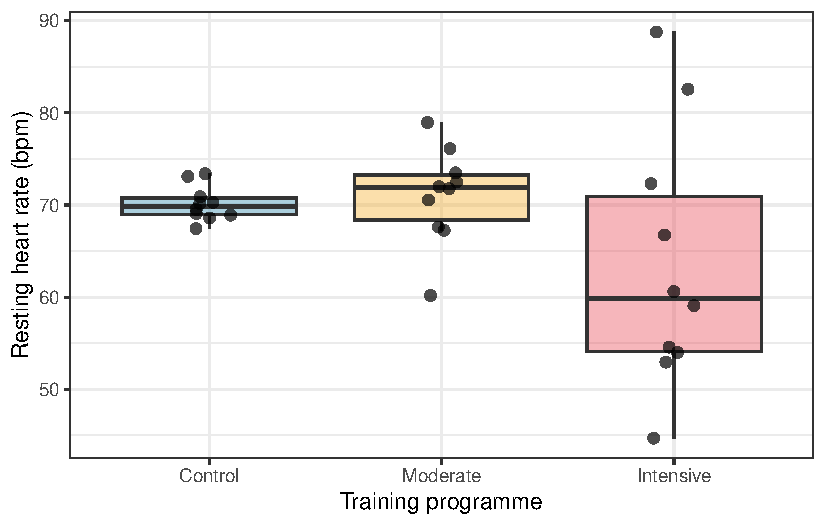
\includegraphics[width=0.9\textwidth,height=\textheight]{02b-assumptions_files/figure-pdf/fig-homoscedasticity-plot-1.pdf}

}

\caption{\label{fig-homoscedasticity-plot}Simulated heart rate data from
one realisation of the three-group experiment. The groups share the same
true mean but differ dramatically in their spread. This pattern, wider
scatter in one group than another, is the signature of
heteroscedasticity.}

\end{figure}%

Notice how the control group clusters tightly while the intensive group
spreads widely up and down. This is exactly the pattern that violates
the homoscedasticity assumption and distorts the standard \(F\) test.

\subsection{How to check the
assumption}\label{how-to-check-the-assumption}

There are two complementary approaches, and you should use both.

\begin{itemize}
\item
  \textbf{Graphically}: always the first step. A boxplot or a plot of
  residuals against fitted values will reveal unequal spread across
  groups far more intuitively than any test statistic. If the boxes in
  your boxplot differ dramatically in height, or if the residual spread
  fans out as fitted values increase, heteroscedasticity is likely.
\item
  \textbf{Formally}: the most commonly used test is \textbf{Levene's
  test}, which tests the null hypothesis that all group variances are
  equal. In R:
\end{itemize}

\begin{Shaded}
\begin{Highlighting}[]
\CommentTok{\# install.packages("car") if not already installed}
\FunctionTok{library}\NormalTok{(car)}
\end{Highlighting}
\end{Shaded}

\begin{verbatim}
#> Loading required package: carData
\end{verbatim}

\begin{Shaded}
\begin{Highlighting}[]
\FunctionTok{leveneTest}\NormalTok{(y }\SpecialCharTok{\textasciitilde{}}\NormalTok{ group, }\AttributeTok{data =}\NormalTok{ df\_plot)}
\end{Highlighting}
\end{Shaded}

\begin{verbatim}
#> Levene's Test for Homogeneity of Variance (center = median)
#>       Df F value   Pr(>F)   
#> group  2  6.7529 0.004187 **
#>       27                    
#> ---
#> Signif. codes:  0 '***' 0.001 '**' 0.01 '*' 0.05 '.' 0.1 ' ' 1
\end{verbatim}

A significant result (\(p < 0.05\)) suggests that the variances are not
equal and that standard ANOVA should be used with caution. Note however
that Levene's test, like all formal tests of assumptions, is sensitive
to sample size: with very large samples it will flag trivially small
differences in variance as significant, while with very small samples it
may miss substantial heteroscedasticity. The graphical check should
always come first.

\subsection{What to do when the assumption is
violated}\label{what-to-do-when-the-assumption-is-violated}

Fortunately, several straightforward options are available.

\textbf{Welch's ANOVA} is the simplest and most recommended solution for
the one-way case. It relaxes the equal-variance assumption by adjusting
the degrees of freedom of the \(F\) test, and it performs well even when
variances are equal: making it a sensible default in many situations. In
R it is a single argument change:

\begin{Shaded}
\begin{Highlighting}[]
\CommentTok{\# Standard ANOVA}
\FunctionTok{summary}\NormalTok{(}\FunctionTok{aov}\NormalTok{(y }\SpecialCharTok{\textasciitilde{}}\NormalTok{ group, }\AttributeTok{data =}\NormalTok{ df\_plot))}
\end{Highlighting}
\end{Shaded}

\begin{verbatim}
#>             Df Sum Sq Mean Sq F value Pr(>F)
#> group        2  327.4  163.68   2.177  0.133
#> Residuals   27 2029.7   75.17
\end{verbatim}

\begin{Shaded}
\begin{Highlighting}[]
\CommentTok{\# Welch\textquotesingle{}s ANOVA, preferred when variances may differ}
\FunctionTok{oneway.test}\NormalTok{(y }\SpecialCharTok{\textasciitilde{}}\NormalTok{ group, }\AttributeTok{data =}\NormalTok{ df\_plot, }\AttributeTok{var.equal =} \ConstantTok{FALSE}\NormalTok{)}
\end{Highlighting}
\end{Shaded}

\begin{verbatim}
#> 
#>  One-way analysis of means (not assuming equal variances)
#> 
#> data:  y and group
#> F = 1.18, num df = 2.000, denom df = 13.596, p-value = 0.3369
\end{verbatim}

\textbf{Variance-stabilising transformations} are worth considering when
heteroscedasticity has a systematic pattern. If variability tends to
increase with the mean, a common situation with count data or strictly
positive measurements, a log transformation often brings the variances
into approximate equality:

\begin{Shaded}
\begin{Highlighting}[]
\NormalTok{df\_plot}\SpecialCharTok{$}\NormalTok{log\_y }\OtherTok{\textless{}{-}} \FunctionTok{log}\NormalTok{(df\_plot}\SpecialCharTok{$}\NormalTok{y)}
\FunctionTok{oneway.test}\NormalTok{(log\_y }\SpecialCharTok{\textasciitilde{}}\NormalTok{ group, }\AttributeTok{data =}\NormalTok{ df\_plot, }\AttributeTok{var.equal =} \ConstantTok{FALSE}\NormalTok{)}
\end{Highlighting}
\end{Shaded}

\begin{verbatim}
#> 
#>  One-way analysis of means (not assuming equal variances)
#> 
#> data:  log_y and group
#> F = 1.548, num df = 2.000, denom df = 13.517, p-value = 0.2481
\end{verbatim}

Always check whether the transformed values still make biological sense
and whether the transformation has actually equalised the variances
before proceeding.

\subsection{A Note on robustness}\label{a-note-on-robustness}

Standard ANOVA is moderately robust to mild violations of
homoscedasticity, particularly when group sizes are equal. The \(F\)
test begins to behave badly mainly when two conditions coincide: the
variances are very different \emph{and} the group sizes are unequal. In
that situation the combination of an unreliable pooled variance estimate
and an unbalanced design can push the false positive rate far from the
nominal level, as the simulation above illustrates. When in doubt,
Welch's ANOVA costs you almost nothing and protects you against a real
and avoidable source of error.

\section{Normality of Residuals: What It Means and What It
Doesn't}\label{normality-of-residuals-what-it-means-and-what-it-doesnt}

\subsection{What Does the Assumption
Say?}\label{what-does-the-assumption-say-1}

ANOVA assumes that the residuals, the differences between each observed
value and its group mean, are approximately normally distributed. It is
worth being precise about this from the start, because the assumption is
frequently misunderstood in two important ways.

\textbf{First misunderstanding:} students often believe that ANOVA
requires the raw observations to be normally distributed. This is not
quite right. What must be approximately normal are the \emph{residuals},
not the raw data. If your groups have very different means, the overall
distribution of all observations pooled together will naturally look
non-normal even when the residuals within each group are perfectly
well-behaved. Always examine the residuals, not the raw values.

\textbf{Second misunderstanding:} students often treat normality as a
strict prerequisite, checking it anxiously and abandoning ANOVA at the
slightest deviation. As we will show below with simulations, this
caution is largely unwarranted for one-way ANOVA. The test is remarkably
robust to departures from normality, and the cases where normality
genuinely matters are more specific than most textbooks suggest.

\subsection{What is a residual?}\label{what-is-a-residual}

The residual for observation \(i\) in group \(j\) is:

\[e_{ij} = y_{ij} - \bar{y}_j\]

where \(y_{ij}\) is the observed value and \(\bar{y}_j\) is the mean of
group \(j\). The residual captures everything about an observation that
group membership cannot explain. If the model is doing its job, these
leftovers should look like random draws from a distribution centred on
zero.

\subsection{Why residuals, not raw
data?}\label{sec-why-residuals-not-raw-data}

This point confuses almost every student encountering ANOVA for the
first time, so it is worth working through carefully.

\subsubsection{Start with what ANOVA actually
models}\label{start-with-what-anova-actually-models}

Recall the fundamental equation of ANOVA:

\[y_{ij} = \mu + \alpha_j + \varepsilon_{ij}\]

where \(y_{ij}\) is the observed value, \(\mu\) is the grand mean,
\(\alpha_j\) is the effect of group \(j\), and \(\varepsilon_{ij}\) is
the residual --- the part of the observation that the model cannot
explain. The normality assumption is a statement about
\(\varepsilon_{ij}\), the residual, not about \(y_{ij}\), the raw
observation. To understand why, we need to understand what the residual
actually is.

\subsubsection{The residual is what remains after removing the group
effect}\label{the-residual-is-what-remains-after-removing-the-group-effect}

Think of it this way. You measure the height of 12 wheat plants across
three fertiliser groups. The plants in the nitrogen group are, on
average, taller than those in the control group. If you look at the raw
heights of all 12 plants pooled together, you will see a spread that
reflects two things simultaneously: the genuine differences between
fertiliser groups, and the random scatter within each group. These two
sources of variation are tangled together in the raw data.

The residual disentangles them. When you subtract each plant's group
mean from its observed height, you remove the group effect entirely.
What remains, the residual, is pure within-group scatter, stripped of
any systematic influence of the treatment. It is this pure scatter that
ANOVA assumes to be normally distributed.

A simple analogy: imagine you are measuring the heights of students from
three different countries, where average heights differ between
countries. If you pool all students together and look at the height
distribution, you might see a wide, irregular spread reflecting the mix
of nationalities. But if you subtract each student's national average
first, the residuals, the deviation of each student from their national
average, will look much more like a single clean normal distribution.
The raw data were non-normal not because heights within any country were
non-normal, but because you were mixing apples and oranges.

\subsubsection{A concrete simulation}\label{a-concrete-simulation}

The code below makes this vivid. We simulate three groups with very
different means but identical, perfectly normal within-group scatter. We
then plot both the raw data and the residuals and examine their
distributions.

\begin{Shaded}
\begin{Highlighting}[]
\FunctionTok{library}\NormalTok{(ggplot2)}
\FunctionTok{library}\NormalTok{(patchwork)}

\FunctionTok{set.seed}\NormalTok{(}\DecValTok{42}\NormalTok{)}

\NormalTok{n }\OtherTok{\textless{}{-}} \DecValTok{30}
\NormalTok{group\_means }\OtherTok{\textless{}{-}} \FunctionTok{c}\NormalTok{(}\DecValTok{10}\NormalTok{, }\DecValTok{25}\NormalTok{, }\DecValTok{45}\NormalTok{)   }\CommentTok{\# very different group means}
\NormalTok{sigma }\OtherTok{\textless{}{-}} \DecValTok{3} \CommentTok{\# identical within{-}group sd, normal scatter}

\NormalTok{group }\OtherTok{\textless{}{-}} \FunctionTok{factor}\NormalTok{(}\FunctionTok{rep}\NormalTok{(}\FunctionTok{c}\NormalTok{(}\StringTok{"Control"}\NormalTok{, }\StringTok{"Nitrogen"}\NormalTok{, }\StringTok{"Phosphorus"}\NormalTok{), }\AttributeTok{each =}\NormalTok{ n))}
\NormalTok{y }\OtherTok{\textless{}{-}} \FunctionTok{c}\NormalTok{(}
  \FunctionTok{rnorm}\NormalTok{(n, }\AttributeTok{mean =}\NormalTok{ group\_means[}\DecValTok{1}\NormalTok{], }\AttributeTok{sd =}\NormalTok{ sigma), }\CommentTok{\# control}
  \FunctionTok{rnorm}\NormalTok{(n, }\AttributeTok{mean =}\NormalTok{ group\_means[}\DecValTok{2}\NormalTok{], }\AttributeTok{sd =}\NormalTok{ sigma), }\CommentTok{\# nitrogen}
  \FunctionTok{rnorm}\NormalTok{(n, }\AttributeTok{mean =}\NormalTok{ group\_means[}\DecValTok{3}\NormalTok{], }\AttributeTok{sd =}\NormalTok{ sigma) }\CommentTok{\# phosphorus}
\NormalTok{)}

\NormalTok{df }\OtherTok{\textless{}{-}} \FunctionTok{data.frame}\NormalTok{(y, group)}

\CommentTok{\# Compute residuals by subtracting each group mean}
\NormalTok{df}\SpecialCharTok{$}\NormalTok{residual }\OtherTok{\textless{}{-}}\NormalTok{ df}\SpecialCharTok{$}\NormalTok{y }\SpecialCharTok{{-}} \FunctionTok{ave}\NormalTok{(df}\SpecialCharTok{$}\NormalTok{y, df}\SpecialCharTok{$}\NormalTok{group, }\AttributeTok{FUN =}\NormalTok{ mean)}

\NormalTok{p1 }\OtherTok{\textless{}{-}} \FunctionTok{ggplot}\NormalTok{(df, }\FunctionTok{aes}\NormalTok{(}\AttributeTok{x =}\NormalTok{ y, }\AttributeTok{fill =}\NormalTok{ group)) }\SpecialCharTok{+}
  \FunctionTok{geom\_histogram}\NormalTok{(}\AttributeTok{binwidth =} \DecValTok{2}\NormalTok{, }\AttributeTok{colour =} \StringTok{"white"}\NormalTok{, }\AttributeTok{alpha =} \FloatTok{0.8}\NormalTok{) }\SpecialCharTok{+}
  \FunctionTok{scale\_fill\_manual}\NormalTok{(}\AttributeTok{values =} \FunctionTok{c}\NormalTok{(}\StringTok{"\#2E86AB"}\NormalTok{, }\StringTok{"\#F6AE2D"}\NormalTok{, }\StringTok{"\#E84855"}\NormalTok{)) }\SpecialCharTok{+}
  \FunctionTok{labs}\NormalTok{(}\AttributeTok{title =} \StringTok{"Raw data (by group)"}\NormalTok{, }\AttributeTok{x =} \StringTok{"Plant height (cm)"}\NormalTok{, }\AttributeTok{y =} \StringTok{"Count"}\NormalTok{) }\SpecialCharTok{+}
  \FunctionTok{theme\_bw}\NormalTok{() }\SpecialCharTok{+}
  \FunctionTok{theme}\NormalTok{(}\AttributeTok{legend.position =} \StringTok{"none"}\NormalTok{)}

\NormalTok{p2 }\OtherTok{\textless{}{-}} \FunctionTok{ggplot}\NormalTok{(df, }\FunctionTok{aes}\NormalTok{(}\AttributeTok{x =}\NormalTok{ y)) }\SpecialCharTok{+}
  \FunctionTok{geom\_histogram}\NormalTok{(}\AttributeTok{binwidth =} \DecValTok{2}\NormalTok{, }\AttributeTok{fill =} \StringTok{"\#555555"}\NormalTok{, }\AttributeTok{colour =} \StringTok{"white"}\NormalTok{) }\SpecialCharTok{+}
  \FunctionTok{labs}\NormalTok{(}\AttributeTok{title =} \StringTok{"Raw data (all groups pooled)"}\NormalTok{, }\AttributeTok{x =} \StringTok{"Plant height (cm)"}\NormalTok{, }\AttributeTok{y =} \StringTok{"Count"}\NormalTok{) }\SpecialCharTok{+}
  \FunctionTok{theme\_bw}\NormalTok{()}

\NormalTok{p3 }\OtherTok{\textless{}{-}} \FunctionTok{ggplot}\NormalTok{(df, }\FunctionTok{aes}\NormalTok{(}\AttributeTok{x =}\NormalTok{ residual, }\AttributeTok{fill =}\NormalTok{ group)) }\SpecialCharTok{+}
  \FunctionTok{geom\_histogram}\NormalTok{(}\AttributeTok{binwidth =} \DecValTok{1}\NormalTok{, }\AttributeTok{colour =} \StringTok{"white"}\NormalTok{, }\AttributeTok{alpha =} \FloatTok{0.8}\NormalTok{) }\SpecialCharTok{+}
  \FunctionTok{scale\_fill\_manual}\NormalTok{(}\AttributeTok{values =} \FunctionTok{c}\NormalTok{(}\StringTok{"\#2E86AB"}\NormalTok{, }\StringTok{"\#F6AE2D"}\NormalTok{, }\StringTok{"\#E84855"}\NormalTok{)) }\SpecialCharTok{+}
  \FunctionTok{labs}\NormalTok{(}\AttributeTok{title =} \StringTok{"Residuals (by group)"}\NormalTok{, }\AttributeTok{x =} \StringTok{"Residual"}\NormalTok{, }\AttributeTok{y =} \StringTok{"Count"}\NormalTok{) }\SpecialCharTok{+}
  \FunctionTok{theme\_bw}\NormalTok{() }\SpecialCharTok{+}
  \FunctionTok{theme}\NormalTok{(}\AttributeTok{legend.position =} \StringTok{"none"}\NormalTok{)}

\NormalTok{p4 }\OtherTok{\textless{}{-}} \FunctionTok{ggplot}\NormalTok{(df, }\FunctionTok{aes}\NormalTok{(}\AttributeTok{x =}\NormalTok{ residual)) }\SpecialCharTok{+}
  \FunctionTok{geom\_histogram}\NormalTok{(}\AttributeTok{binwidth =} \DecValTok{1}\NormalTok{, }\AttributeTok{fill =} \StringTok{"\#555555"}\NormalTok{, }\AttributeTok{colour =} \StringTok{"white"}\NormalTok{) }\SpecialCharTok{+}
  \FunctionTok{labs}\NormalTok{(}\AttributeTok{title =} \StringTok{"Residuals (all groups pooled)"}\NormalTok{, }\AttributeTok{x =} \StringTok{"Residual"}\NormalTok{, }\AttributeTok{y =} \StringTok{"Count"}\NormalTok{) }\SpecialCharTok{+}
  \FunctionTok{theme\_bw}\NormalTok{()}

\NormalTok{(p1 }\SpecialCharTok{+}\NormalTok{ p3) }\SpecialCharTok{/}\NormalTok{ (p2 }\SpecialCharTok{+}\NormalTok{ p4)}
\end{Highlighting}
\end{Shaded}

\begin{figure}[H]

\centering{

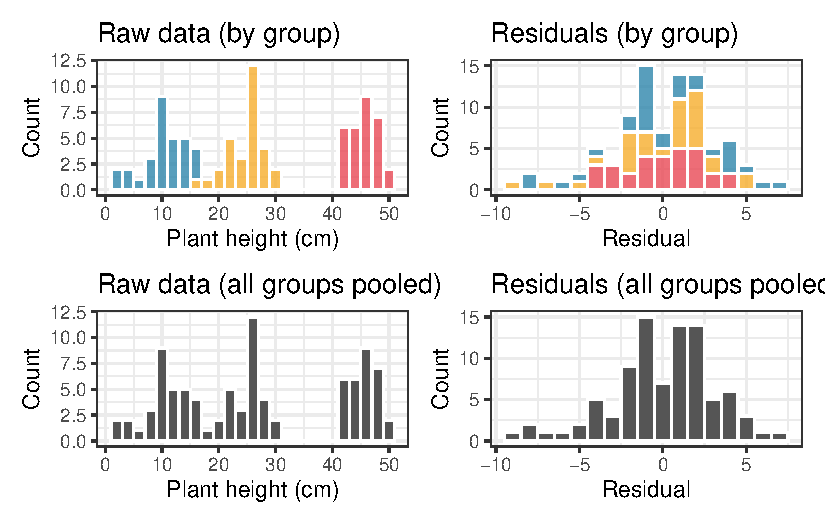
\includegraphics[width=0.9\textwidth,height=\textheight]{02b-assumptions_files/figure-pdf/fig-residuals-vs-raw-1.pdf}

}

\caption{\label{fig-residuals-vs-raw}Left column: the raw observations
from three groups with very different means. The pooled distribution
(bottom left) looks nothing like a normal distribution, it is wide and
irregular. Right column: the residuals after subtracting each group
mean. The pooled residual distribution (bottom right) is clearly normal,
because the within-group scatter was normal all along. ANOVA only
requires the right column to be normal.}

\end{figure}%

Look carefully at the bottom row. The pooled raw data (bottom left)
shows three separate humps, one for each group, spread across a wide
range. This looks nothing like a normal distribution, and a Shapiro-Wilk
test on the raw data would resoundingly reject normality. Yet the data
were generated with perfectly normal within-group scatter. The apparent
non-normality of the raw data is entirely an artefact of the groups
having different means. It tells you nothing about whether ANOVA is
appropriate.

The pooled residuals (bottom right), by contrast, form a single clean
bell-shaped distribution centred on zero. This is because subtracting
the group means has removed the between-group differences, leaving only
the within-group scatter, which was normal by construction.

\subsubsection{\texorpdfstring{Why does the \(F\) test need normal
residuals?}{Why does the F test need normal residuals?}}\label{why-does-the-f-test-need-normal-residuals}

The \(F\) statistic is a ratio of two variance estimates. The
mathematical theory that tells us how \(F\) behaves under the null
hypothesis, and therefore allows us to compute a \(p\)-value, was
derived under the assumption that the residuals are normally
distributed.

\begin{tcolorbox}[enhanced jigsaw, title=\textcolor{quarto-callout-tip-color}{\faLightbulb}\hspace{0.5em}{Show me the maths!}, opacityback=0, bottomtitle=1mm, leftrule=.75mm, breakable, toprule=.15mm, colframe=quarto-callout-tip-color-frame, titlerule=0mm, rightrule=.15mm, toptitle=1mm, arc=.35mm, colback=white, left=2mm, colbacktitle=quarto-callout-tip-color!10!white, opacitybacktitle=0.6, coltitle=black, bottomrule=.15mm]

Want to understand the precise mathematical chain that connects normal
residuals to the F distribution? See
Section~\ref{sec-ftest-normality-maths} in Appendix A.

\end{tcolorbox}

Specifically, when residuals are normal, the two variance estimates in
the \(F\) ratio follow chi-squared distributions, and the ratio of two
chi-squared variables follows an \(F\) distribution. It is this chain of
reasoning that connects your data to the \(p\)-value printed by R.

If the residuals are not normal, this chain is broken, at least in
principle. The \(F\) statistic may no longer follow the \(F\)
distribution under the null hypothesis, and the \(p\)-value becomes an
approximation whose quality depends on how far from normality the
residuals actually are. As the simulations in the previous section
showed, this approximation tends to remain very good for one-way ANOVA
even under substantial departures from normality. But understanding
\emph{why} normality is the requirement, rather than just memorising
that it is, helps you make informed judgements about when to worry and
when not to.

\subsubsection{The practical
consequence}\label{the-practical-consequence}

Never apply the Shapiro-Wilk test or draw a Q-Q plot on your raw
observations. Always fit the ANOVA model first, extract the residuals,
and examine those. In R this is a single line:

\begin{Shaded}
\begin{Highlighting}[]
\NormalTok{fit }\OtherTok{\textless{}{-}} \FunctionTok{aov}\NormalTok{(y }\SpecialCharTok{\textasciitilde{}}\NormalTok{ group, }\AttributeTok{data =}\NormalTok{ df)}

\CommentTok{\# Extract residuals}
\NormalTok{res }\OtherTok{\textless{}{-}} \FunctionTok{residuals}\NormalTok{(fit)}

\CommentTok{\# Q{-}Q plot}
\FunctionTok{ggplot}\NormalTok{(fit, }\FunctionTok{aes}\NormalTok{(}\AttributeTok{sample =}\NormalTok{ res)) }\SpecialCharTok{+}
  \FunctionTok{stat\_qq}\NormalTok{(}\AttributeTok{colour =} \StringTok{"\#2E86AB"}\NormalTok{, }\AttributeTok{size =} \DecValTok{2}\NormalTok{) }\SpecialCharTok{+}
  \FunctionTok{stat\_qq\_line}\NormalTok{(}\AttributeTok{colour =} \StringTok{"\#E84855"}\NormalTok{, }\AttributeTok{linewidth =} \FloatTok{0.8}\NormalTok{) }\SpecialCharTok{+} 
  \FunctionTok{labs}\NormalTok{(}\AttributeTok{x =} \StringTok{"Theoretical quantiles"}\NormalTok{, }\AttributeTok{y =} \StringTok{"Sample quantiles"}\NormalTok{) }\SpecialCharTok{+}
  \FunctionTok{theme\_bw}\NormalTok{()}

\CommentTok{\# Formal test}
\FunctionTok{shapiro.test}\NormalTok{(res)}
\end{Highlighting}
\end{Shaded}

\begin{verbatim}
#> 
#>  Shapiro-Wilk normality test
#> 
#> data:  res
#> W = 0.97768, p-value = 0.124
\end{verbatim}

\begin{figure}[H]

\centering{

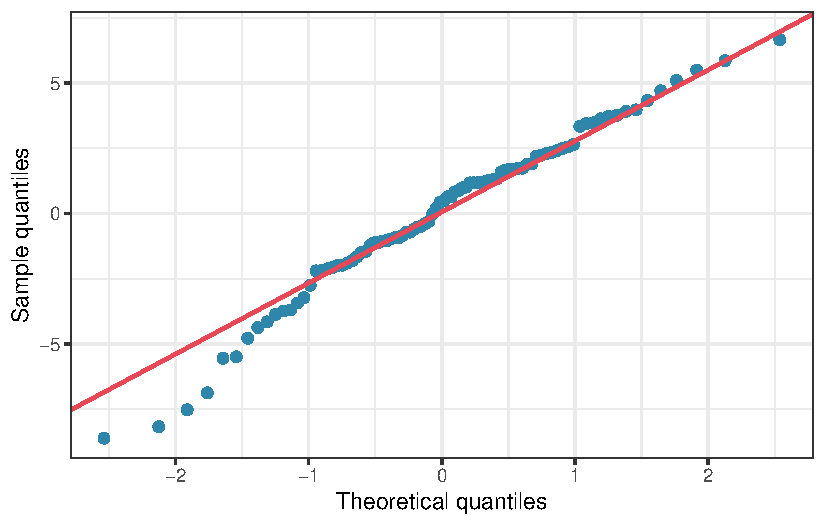
\includegraphics[width=0.9\textwidth,height=\textheight]{02b-assumptions_files/figure-pdf/fig-extract-residuals-1.pdf}

}

\caption{\label{fig-extract-residuals}Residuals QQ-plot showing minor
divergence from normality.}

\end{figure}%

If you had applied \texttt{shapiro.test(df\$y)} to the raw data in our
simulated example above, you would have concluded that the data were
catastrophically non-normal and that ANOVA was inappropriate, the exact
wrong conclusion, since the data were generated with perfectly normal
within-group scatter.

Checking residuals rather than raw values is not a technicality. It is
the difference between asking the right question and the wrong one.

\subsection{How serious is the violation, really? A
simulation}\label{how-serious-is-the-violation-really-a-simulation}

Rather than asserting that normality matters, let us measure how much it
matters directly. The code below generates data from distributions of
increasing non-normality, specifically \(t\)-distributions with
decreasing degrees of freedom (df), which range from nearly normal (high
df) to heavy-tailed (low df), and measures the false positive rate of
ANOVA in each case.

\begin{Shaded}
\begin{Highlighting}[]
\FunctionTok{set.seed}\NormalTok{(}\DecValTok{42}\NormalTok{)}

\NormalTok{n\_sim }\OtherTok{\textless{}{-}} \DecValTok{5000}
\NormalTok{alpha }\OtherTok{\textless{}{-}} \FloatTok{0.05}
\NormalTok{n }\OtherTok{\textless{}{-}} \DecValTok{8}  \CommentTok{\# small group size, where normality matters most}
\NormalTok{df\_values }\OtherTok{\textless{}{-}} \FunctionTok{c}\NormalTok{(}\DecValTok{2}\NormalTok{, }\DecValTok{3}\NormalTok{, }\DecValTok{4}\NormalTok{, }\DecValTok{5}\NormalTok{, }\DecValTok{10}\NormalTok{, }\DecValTok{30}\NormalTok{, }\ConstantTok{Inf}\NormalTok{)  }\CommentTok{\# Inf = exactly normal}

\NormalTok{results }\OtherTok{\textless{}{-}} \FunctionTok{data.frame}\NormalTok{(}
  \AttributeTok{distribution =} \FunctionTok{c}\NormalTok{(}\StringTok{"t (df=2)"}\NormalTok{, }\StringTok{"t (df=3)"}\NormalTok{, }\StringTok{"t (df=4)"}\NormalTok{,}
                   \StringTok{"t (df=5)"}\NormalTok{, }\StringTok{"t (df=10)"}\NormalTok{, }\StringTok{"t (df=30)"}\NormalTok{, }\StringTok{"Normal"}\NormalTok{),}
  \AttributeTok{df =}\NormalTok{ df\_values,}
  \AttributeTok{fpr =} \ConstantTok{NA}
\NormalTok{)}

\ControlFlowTok{for}\NormalTok{ (j }\ControlFlowTok{in} \FunctionTok{seq\_along}\NormalTok{(df\_values)) \{}
\NormalTok{  p\_vals }\OtherTok{\textless{}{-}} \FunctionTok{numeric}\NormalTok{(n\_sim)}
  \ControlFlowTok{for}\NormalTok{ (i }\ControlFlowTok{in} \FunctionTok{seq\_len}\NormalTok{(n\_sim)) \{}
    \CommentTok{\# Draw from t{-}distribution (Inf df = normal)}
\NormalTok{    y }\OtherTok{\textless{}{-}} \ControlFlowTok{if}\NormalTok{ (}\FunctionTok{is.infinite}\NormalTok{(df\_values[j])) \{}
      \FunctionTok{rnorm}\NormalTok{(}\DecValTok{3} \SpecialCharTok{*}\NormalTok{ n)}
\NormalTok{    \} }\ControlFlowTok{else}\NormalTok{ \{}
      \FunctionTok{rt}\NormalTok{(}\DecValTok{3} \SpecialCharTok{*}\NormalTok{ n, }\AttributeTok{df =}\NormalTok{ df\_values[j])}
\NormalTok{    \}}
    
\NormalTok{    group    }\OtherTok{\textless{}{-}} \FunctionTok{factor}\NormalTok{(}\FunctionTok{rep}\NormalTok{(}\FunctionTok{c}\NormalTok{(}\StringTok{"A"}\NormalTok{, }\StringTok{"B"}\NormalTok{, }\StringTok{"C"}\NormalTok{), }\AttributeTok{each =}\NormalTok{ n))}
\NormalTok{    p\_vals[i] }\OtherTok{\textless{}{-}} \FunctionTok{summary}\NormalTok{(}
      \FunctionTok{aov}\NormalTok{(y }\SpecialCharTok{\textasciitilde{}}\NormalTok{ group, }\AttributeTok{data =} \FunctionTok{data.frame}\NormalTok{(y, group))}
\NormalTok{    )[[}\DecValTok{1}\NormalTok{]][[}\StringTok{"Pr(\textgreater{}F)"}\NormalTok{]][}\DecValTok{1}\NormalTok{]}
\NormalTok{  \}}
  
\NormalTok{  results}\SpecialCharTok{$}\NormalTok{fpr[j] }\OtherTok{\textless{}{-}} \FunctionTok{mean}\NormalTok{(p\_vals }\SpecialCharTok{\textless{}}\NormalTok{ alpha)}
\NormalTok{\}}
\end{Highlighting}
\end{Shaded}

All three groups share the same mean, so every significant result is a
false positive.

\begin{Shaded}
\begin{Highlighting}[]
\FunctionTok{print}\NormalTok{(results)}
\end{Highlighting}
\end{Shaded}

\begin{verbatim}
#>   distribution  df    fpr
#> 1     t (df=2)   2 0.0326
#> 2     t (df=3)   3 0.0422
#> 3     t (df=4)   4 0.0424
#> 4     t (df=5)   5 0.0466
#> 5    t (df=10)  10 0.0476
#> 6    t (df=30)  30 0.0508
#> 7       Normal Inf 0.0452
\end{verbatim}

The result is striking: even with extremely heavy-tailed distributions
(\(df = 2\) is very far from normal), the false positive rate never
strays far from the nominal 5\%. If anything, ANOVA becomes slightly
\emph{conservative} under heavy tails, the false positive rate drops a
little below 0.05, meaning the test becomes harder to reject than it
should be, not easier. This is the opposite of what most students
expect.

Let us visualise this across the range of distributions tested:

\begin{Shaded}
\begin{Highlighting}[]
\FunctionTok{library}\NormalTok{(ggplot2)}

\CommentTok{\# Monte Carlo confidence interval for the false positive rate}
\CommentTok{\# given n\_sim = 5000 simulations}
\NormalTok{mc\_lower }\OtherTok{\textless{}{-}} \FunctionTok{qbinom}\NormalTok{(}\FloatTok{0.025}\NormalTok{, n\_sim, alpha) }\SpecialCharTok{/}\NormalTok{ n\_sim}
\NormalTok{mc\_upper }\OtherTok{\textless{}{-}} \FunctionTok{qbinom}\NormalTok{(}\FloatTok{0.975}\NormalTok{, n\_sim, alpha) }\SpecialCharTok{/}\NormalTok{ n\_sim}

\NormalTok{results}\SpecialCharTok{$}\NormalTok{distribution }\OtherTok{\textless{}{-}} \FunctionTok{factor}\NormalTok{(results}\SpecialCharTok{$}\NormalTok{distribution, }\AttributeTok{levels =}\NormalTok{ results}\SpecialCharTok{$}\NormalTok{distribution)}

\FunctionTok{ggplot}\NormalTok{(results, }\FunctionTok{aes}\NormalTok{(}\AttributeTok{x =}\NormalTok{ distribution, }\AttributeTok{y =}\NormalTok{ fpr)) }\SpecialCharTok{+}
  \FunctionTok{annotate}\NormalTok{(}\StringTok{"rect"}\NormalTok{, }\AttributeTok{xmin =} \SpecialCharTok{{-}}\ConstantTok{Inf}\NormalTok{, }\AttributeTok{xmax =} \ConstantTok{Inf}\NormalTok{, }\AttributeTok{ymin =}\NormalTok{ mc\_lower, }\AttributeTok{ymax =}\NormalTok{ mc\_upper, }\AttributeTok{fill =} \StringTok{"\#2E86AB"}\NormalTok{, }\AttributeTok{alpha =} \FloatTok{0.15}\NormalTok{) }\SpecialCharTok{+}
  \FunctionTok{geom\_hline}\NormalTok{(}\AttributeTok{yintercept =}\NormalTok{ alpha, }\AttributeTok{linetype =} \StringTok{"dashed"}\NormalTok{, }\AttributeTok{colour =} \StringTok{"red"}\NormalTok{, }\AttributeTok{linewidth =} \FloatTok{0.8}\NormalTok{) }\SpecialCharTok{+}
  \FunctionTok{geom\_point}\NormalTok{(}\AttributeTok{size =} \DecValTok{3}\NormalTok{, }\AttributeTok{colour =} \StringTok{"\#2E86AB"}\NormalTok{) }\SpecialCharTok{+}
  \FunctionTok{geom\_line}\NormalTok{(}\FunctionTok{aes}\NormalTok{(}\AttributeTok{group =} \DecValTok{1}\NormalTok{), }\AttributeTok{colour =} \StringTok{"\#2E86AB"}\NormalTok{, }\AttributeTok{linewidth =} \FloatTok{0.8}\NormalTok{) }\SpecialCharTok{+}
  \FunctionTok{scale\_y\_continuous}\NormalTok{(}\AttributeTok{limits =} \FunctionTok{c}\NormalTok{(}\DecValTok{0}\NormalTok{, }\FloatTok{0.10}\NormalTok{), }\AttributeTok{labels =}\NormalTok{ scales}\SpecialCharTok{::}\FunctionTok{percent\_format}\NormalTok{(}\AttributeTok{accuracy =} \DecValTok{1}\NormalTok{)) }\SpecialCharTok{+}
  \FunctionTok{labs}\NormalTok{(}\AttributeTok{x =} \StringTok{"Residual distribution (left = heavy{-}tailed, right = normal)"}\NormalTok{, }\AttributeTok{y =} \StringTok{"False positive rate"}\NormalTok{) }\SpecialCharTok{+}
  \FunctionTok{theme\_bw}\NormalTok{() }\SpecialCharTok{+}
  \FunctionTok{theme}\NormalTok{(}\AttributeTok{axis.text.x =} \FunctionTok{element\_text}\NormalTok{(}\AttributeTok{angle =} \DecValTok{30}\NormalTok{, }\AttributeTok{hjust =} \DecValTok{1}\NormalTok{))}
\end{Highlighting}
\end{Shaded}

\begin{figure}[H]

\centering{

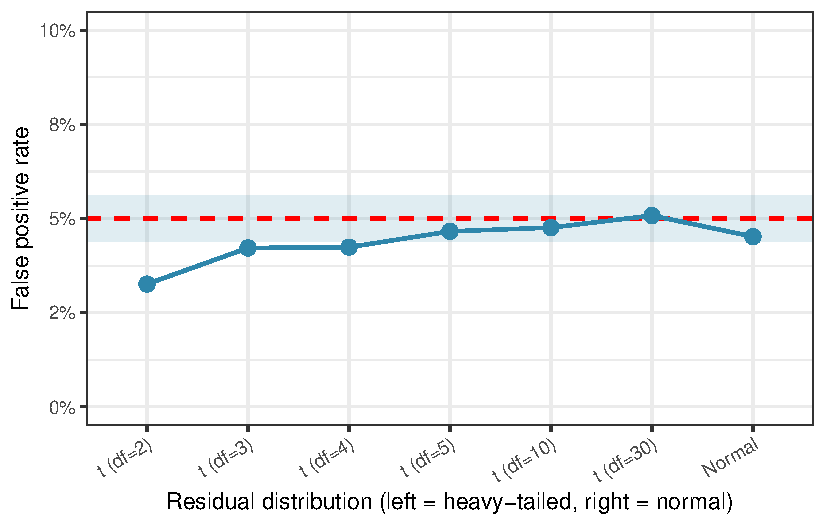
\includegraphics[width=0.9\textwidth,height=\textheight]{02b-assumptions_files/figure-pdf/fig-normality-robustness-plot-1.pdf}

}

\caption{\label{fig-normality-robustness-plot}False positive rate of
one-way ANOVA under increasing departures from normality
(t-distributions with decreasing degrees of freedom). The dashed red
line marks the nominal 5\% level. The shaded band shows a 95\% Monte
Carlo confidence interval around the target rate. The false positive
rate stays close to 5\% throughout, demonstrating the robustness of
ANOVA to non-normality.}

\end{figure}%

All points fall within or very close to the Monte Carlo confidence band
around the 5\% target, the expected range of sampling variation given
5000 simulations. ANOVA is not merely tolerating non-normality here; it
is genuinely indifferent to it, at least in terms of false positive
control.

\subsection{So why does anyone check
normality?}\label{so-why-does-anyone-check-normality}

If ANOVA is this robust, why do textbooks, and this one, discuss
normality at all? There are three legitimate reasons.

\textbf{Outliers are the real concern.} The distributions above are
symmetric and heavy-tailed, but they do not contain the kind of
isolated, extreme outlier that arises from a data entry error, a broken
instrument, or a single anomalous individual. A genuine outlier, say one
plant that grew ten times taller than all others because it was
accidentally given a growth hormone, will dramatically inflate the
within-group variance, absorbing variation that should be attributed to
the treatment. The result is not a false positive but a \textbf{false
negative}: a real treatment effect that the test fails to detect because
the noise floor has been artificially raised. A Q-Q plot will reveal
this outlier immediately.

\textbf{Normality matters more in complex designs.} The robustness
demonstrated above applies cleanly to the balanced one-way ANOVA. In
unbalanced designs, two-way ANOVAs, repeated measures, and mixed models,
departures from normality interact with other features of the design in
ways that are harder to predict and can be more consequential. Good
habits formed in the one-way case carry over to these more demanding
situations.

\textbf{Confidence intervals and post-hoc tests are more sensitive.}
Even when the \(F\) test itself is robust, the confidence intervals
around group means and the \(p\)-values from post-hoc comparisons rely
on the same normality assumption and may be less trustworthy when it is
badly violated.

\subsection{How to Check Residuals in
Practice}\label{how-to-check-residuals-in-practice}

The Q-Q plot remains the best practical tool, not to decide whether to
run ANOVA, but to spot outliers and gross departures that warrant
investigation.

\begin{Shaded}
\begin{Highlighting}[]
\FunctionTok{library}\NormalTok{(ggplot2)}
\FunctionTok{library}\NormalTok{(patchwork)}

\FunctionTok{set.seed}\NormalTok{(}\DecValTok{7}\NormalTok{)}

\NormalTok{n }\OtherTok{\textless{}{-}} \DecValTok{8}
\NormalTok{group }\OtherTok{\textless{}{-}} \FunctionTok{factor}\NormalTok{(}\FunctionTok{rep}\NormalTok{(}\FunctionTok{c}\NormalTok{(}\StringTok{"Control"}\NormalTok{, }\StringTok{"Nitrogen"}\NormalTok{, }\StringTok{"Phosphorus"}\NormalTok{), }\AttributeTok{each =}\NormalTok{ n))}

\CommentTok{\# Clean data, normal residuals}
\NormalTok{y\_clean }\OtherTok{\textless{}{-}} \FunctionTok{rnorm}\NormalTok{(}\DecValTok{3} \SpecialCharTok{*}\NormalTok{ n, }\AttributeTok{mean =} \DecValTok{10}\NormalTok{, }\AttributeTok{sd =} \DecValTok{2}\NormalTok{)}
\NormalTok{fit\_clean }\OtherTok{\textless{}{-}} \FunctionTok{aov}\NormalTok{(y\_clean }\SpecialCharTok{\textasciitilde{}}\NormalTok{ group)}

\CommentTok{\# Contaminated data, one outlier injected}
\NormalTok{y\_outlier }\OtherTok{\textless{}{-}}\NormalTok{ y\_clean}
\NormalTok{y\_outlier[}\DecValTok{1}\NormalTok{] }\OtherTok{\textless{}{-}}\NormalTok{ y\_outlier[}\DecValTok{1}\NormalTok{] }\SpecialCharTok{+} \DecValTok{18}   \CommentTok{\# one extreme value}
\NormalTok{fit\_outlier }\OtherTok{\textless{}{-}} \FunctionTok{aov}\NormalTok{(y\_outlier }\SpecialCharTok{\textasciitilde{}}\NormalTok{ group)}

\NormalTok{res\_df }\OtherTok{\textless{}{-}} \FunctionTok{data.frame}\NormalTok{(}
  \AttributeTok{residuals =} \FunctionTok{c}\NormalTok{(}\FunctionTok{residuals}\NormalTok{(fit\_clean), }\FunctionTok{residuals}\NormalTok{(fit\_outlier)),}
  \AttributeTok{dataset =} \FunctionTok{rep}\NormalTok{(}\FunctionTok{c}\NormalTok{(}\StringTok{"Clean data"}\NormalTok{, }\StringTok{"One outlier added"}\NormalTok{), }\AttributeTok{each =} \DecValTok{3} \SpecialCharTok{*}\NormalTok{ n)}
\NormalTok{)}

\FunctionTok{ggplot}\NormalTok{(res\_df, }\FunctionTok{aes}\NormalTok{(}\AttributeTok{sample =}\NormalTok{ residuals)) }\SpecialCharTok{+}
  \FunctionTok{stat\_qq}\NormalTok{(}\AttributeTok{colour =} \StringTok{"\#2E86AB"}\NormalTok{, }\AttributeTok{size =} \DecValTok{2}\NormalTok{) }\SpecialCharTok{+}
  \FunctionTok{stat\_qq\_line}\NormalTok{(}\AttributeTok{colour =} \StringTok{"\#E84855"}\NormalTok{, }\AttributeTok{linewidth =} \FloatTok{0.8}\NormalTok{) }\SpecialCharTok{+}
  \FunctionTok{facet\_wrap}\NormalTok{(}\SpecialCharTok{\textasciitilde{}}\NormalTok{ dataset) }\SpecialCharTok{+}
  \FunctionTok{labs}\NormalTok{(}\AttributeTok{x =} \StringTok{"Theoretical quantiles"}\NormalTok{, }\AttributeTok{y =} \StringTok{"Sample quantiles"}\NormalTok{) }\SpecialCharTok{+}
  \FunctionTok{theme\_bw}\NormalTok{()}
\end{Highlighting}
\end{Shaded}

\begin{figure}[H]

\centering{

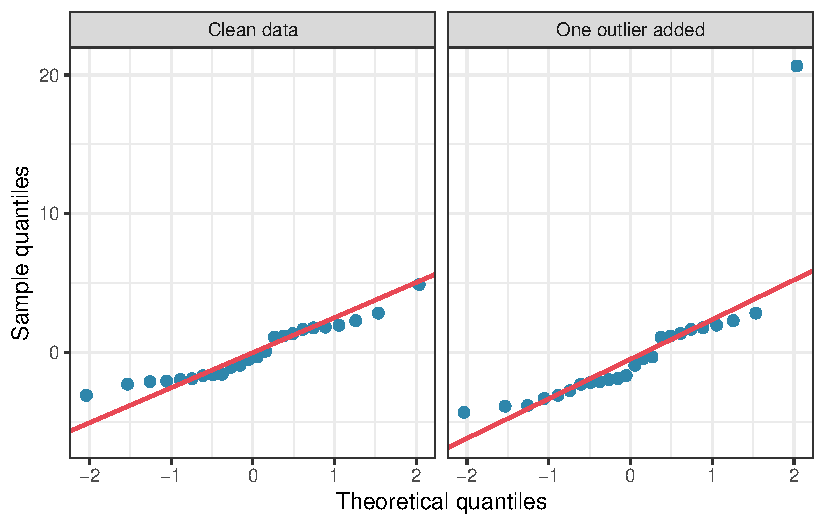
\includegraphics[width=0.9\textwidth,height=\textheight]{02b-assumptions_files/figure-pdf/fig-qq-plot-example-1.pdf}

}

\caption{\label{fig-qq-plot-example}Q-Q plots of ANOVA residuals from
two simulated datasets with n = 8 per group. Left: residuals drawn from
a normal distribution, points fall closely along the diagonal. Right:
the same data with one artificial outlier added to the first group, the
single extreme point is immediately visible at the top right.}

\end{figure}%

The outlier jumps off the page in the Q-Q plot. General non-normality,
by contrast, produces only a gentle curve that is easy to overlook and,
as the simulations show, rarely causes practical problems.

\subsection{What to do when you find an
outlier}\label{what-to-do-when-you-find-an-outlier}

When a Q-Q plot reveals an extreme point, the first step is always to
\textbf{go back to the data}. Ask whether the outlier is:

\begin{itemize}
\tightlist
\item
  A data entry or measurement error: in which case it should be
  corrected or removed with a clear justification recorded.
\item
  A genuine biological observation: in which case removing it is not
  appropriate, but reporting the analysis both with and without it is
  good practice.
\end{itemize}

If outliers are a structural feature of your data rather than isolated
accidents, a robust alternative to ANOVA is available. The
\textbf{Kruskal-Wallis test} replaces raw values with their ranks,
making it insensitive to extreme observations:

\begin{Shaded}
\begin{Highlighting}[]
\FunctionTok{kruskal.test}\NormalTok{(y\_outlier }\SpecialCharTok{\textasciitilde{}}\NormalTok{ group)}
\end{Highlighting}
\end{Shaded}

\begin{verbatim}
#> 
#>  Kruskal-Wallis rank sum test
#> 
#> data:  y_outlier by group
#> Kruskal-Wallis chi-squared = 5.465, df = 2, p-value = 0.06506
\end{verbatim}

\subsection{The key takeaway}\label{the-key-takeaway}

Normality of residuals is the least critical of the three ANOVA
assumptions. For balanced one-way ANOVA, simulations consistently show
that the \(F\) test maintains its false positive rate well even under
substantial departures from normality. So, when doing analysis, check
your residuals with a Q-Q plot, but do so to hunt for outliers and data
problems, not to agonise over gentle curves. In priority, reserve
non-parametric alternatives for situations where outliers are severe and
structural, not as a reflexive response to an imperfect Q-Q plot.

\textbf{The hierarchy of assumptions matters: independence first,
homogeneity of variance second, normality a distant third.}

\section{Additivity and linearity}\label{sec-add-lin}

\subsection{What does the assumption
say?}\label{what-does-the-assumption-say-2}

The linear model underlying ANOVA assumes that the effect of a treatment
adds on to the baseline in a simple, additive way. Formally, the model
says:

\[y_{ij} = \mu + \alpha_j + \varepsilon_{ij}\]

The effect of group \(j\) is \(\alpha_j\), and it is assumed to shift
the response up or down by a fixed amount, independently of everything
else. This is the \textbf{additivity} assumption: the treatment effect
and the error simply add together to produce the observed value. There
are no interactions between the treatment and the background noise, no
situation where the treatment works differently for some individuals
than others.

\subsection{Why does this matter?}\label{why-does-this-matter-1}

Additivity can fail in a subtle but important way. Suppose you are
measuring the effect of three fertilisers on plant yield. For plants
that are already growing vigorously, the fertiliser might produce a
large absolute increase in yield. For plants that are struggling, the
same fertiliser might produce only a small absolute increase. The
treatment effect is not a fixed additive quantity, it depends on the
baseline level of the plant. This is called a
\textbf{treatment-by-individual interaction}, and it violates
additivity.

A more common and detectable form of non-additivity occurs when the
treatment effect is multiplicative rather than additive. Suppose
nitrogen fertiliser multiplies yield by a factor of 1.5, regardless of
baseline. A plant yielding 10g becomes a plant yielding 15g; a plant
yielding 20g becomes a plant yielding 30g. The absolute effect (5g vs
10g) grows with the baseline, which means the within-group variance will
also grow with the group mean, exactly the heteroscedasticity pattern we
discussed in section Section~\ref{sec-homoscedasticity}.
\textbf{Non-additivity and heteroscedasticity often appear together},
which is why a log transformation frequently fixes both problems
simultaneously.

\subsection{Spotting non-additivity}\label{spotting-non-additivity}

The clearest sign of non-additivity is a systematic relationship between
group means and group variances. If the groups with the highest means
also show the most spread, a multiplicative structure is likely. A
simple plot of group standard deviations against group means will reveal
this pattern:

\begin{Shaded}
\begin{Highlighting}[]
\FunctionTok{library}\NormalTok{(ggplot2)}

\FunctionTok{set.seed}\NormalTok{(}\DecValTok{42}\NormalTok{)}
\NormalTok{n }\OtherTok{\textless{}{-}} \DecValTok{15}

\CommentTok{\# Multiplicative model: treatment multiplies the response}
\CommentTok{\# Within{-}group sd grows with the mean: non{-}additive, heteroscedastic}
\NormalTok{group  }\OtherTok{\textless{}{-}} \FunctionTok{factor}\NormalTok{(}\FunctionTok{rep}\NormalTok{(}\FunctionTok{c}\NormalTok{(}\StringTok{"Control"}\NormalTok{, }\StringTok{"Nitrogen"}\NormalTok{, }\StringTok{"Phosphorus"}\NormalTok{), }\AttributeTok{each =}\NormalTok{ n))}
\NormalTok{y\_mult }\OtherTok{\textless{}{-}} \FunctionTok{c}\NormalTok{(}
  \FunctionTok{rnorm}\NormalTok{(n, }\AttributeTok{mean =} \DecValTok{10}\NormalTok{, }\AttributeTok{sd =} \DecValTok{2}\NormalTok{),}
  \FunctionTok{rnorm}\NormalTok{(n, }\AttributeTok{mean =} \DecValTok{20}\NormalTok{, }\AttributeTok{sd =} \DecValTok{4}\NormalTok{),}
  \FunctionTok{rnorm}\NormalTok{(n, }\AttributeTok{mean =} \DecValTok{40}\NormalTok{, }\AttributeTok{sd =} \DecValTok{8}\NormalTok{)}
\NormalTok{)}
\NormalTok{df\_mult }\OtherTok{\textless{}{-}} \FunctionTok{data.frame}\NormalTok{(}\AttributeTok{y =}\NormalTok{ y\_mult, }\AttributeTok{group =}\NormalTok{ group)}

\CommentTok{\# Summarise group means and sds}
\NormalTok{group\_summary }\OtherTok{\textless{}{-}} \FunctionTok{aggregate}\NormalTok{(y }\SpecialCharTok{\textasciitilde{}}\NormalTok{ group, }\AttributeTok{data =}\NormalTok{ df\_mult, }\AttributeTok{FUN =} \ControlFlowTok{function}\NormalTok{(x) }\FunctionTok{c}\NormalTok{(}\AttributeTok{mean =} \FunctionTok{mean}\NormalTok{(x), }\AttributeTok{sd =} \FunctionTok{sd}\NormalTok{(x)))}
\NormalTok{group\_summary }\OtherTok{\textless{}{-}} \FunctionTok{do.call}\NormalTok{(data.frame, group\_summary)}
\FunctionTok{names}\NormalTok{(group\_summary) }\OtherTok{\textless{}{-}} \FunctionTok{c}\NormalTok{(}\StringTok{"group"}\NormalTok{, }\StringTok{"mean"}\NormalTok{, }\StringTok{"sd"}\NormalTok{)}

\FunctionTok{ggplot}\NormalTok{(group\_summary, }\FunctionTok{aes}\NormalTok{(}\AttributeTok{x =}\NormalTok{ mean, }\AttributeTok{y =}\NormalTok{ sd, }\AttributeTok{label =}\NormalTok{ group)) }\SpecialCharTok{+}
  \FunctionTok{geom\_point}\NormalTok{(}\AttributeTok{size =} \DecValTok{4}\NormalTok{, }\AttributeTok{colour =} \StringTok{"\#2E86AB"}\NormalTok{) }\SpecialCharTok{+}
  \FunctionTok{geom\_text}\NormalTok{(}\AttributeTok{vjust =} \SpecialCharTok{{-}}\DecValTok{1}\NormalTok{, }\AttributeTok{colour =} \StringTok{"\#2E86AB"}\NormalTok{) }\SpecialCharTok{+}
  \FunctionTok{geom\_smooth}\NormalTok{(}\AttributeTok{method =} \StringTok{"lm"}\NormalTok{, }\AttributeTok{se =} \ConstantTok{FALSE}\NormalTok{, }\AttributeTok{colour =} \StringTok{"\#E84855"}\NormalTok{, }\AttributeTok{linetype =} \StringTok{"dashed"}\NormalTok{) }\SpecialCharTok{+}
  \FunctionTok{labs}\NormalTok{(}\AttributeTok{x =} \StringTok{"Group mean"}\NormalTok{, }\AttributeTok{y =} \StringTok{"Group standard deviation"}\NormalTok{) }\SpecialCharTok{+}
  \FunctionTok{theme\_bw}\NormalTok{()}
\end{Highlighting}
\end{Shaded}

\begin{figure}[H]

\centering{

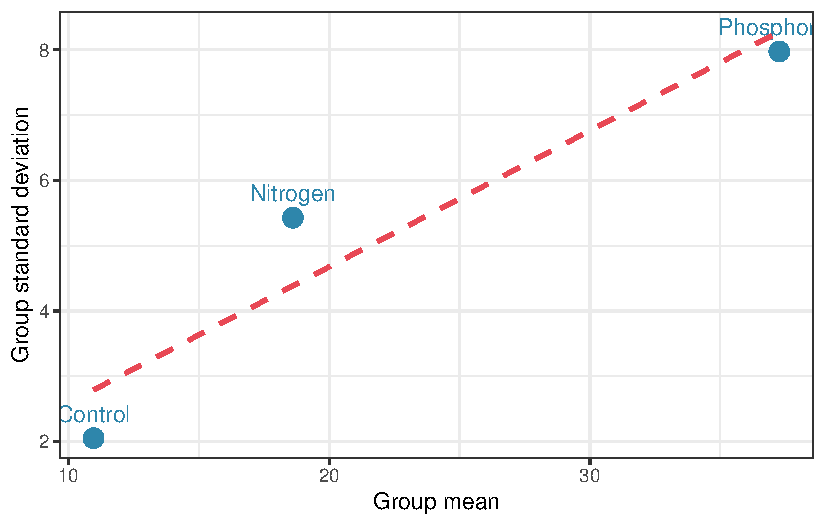
\includegraphics[width=0.9\textwidth,height=\textheight]{02b-assumptions_files/figure-pdf/fig-additivity-check-1.pdf}

}

\caption{\label{fig-additivity-check}Group standard deviation vs group
mean. A positive relationship suggests a multiplicative structure}

\end{figure}%

A positive linear relationship between group mean and group standard
deviation is a reliable diagnostic of multiplicative non-additivity. The
remedy, as before, is a log transformation, which converts
multiplicative relationships into additive ones:

\[\log(y_{ij}) = \mu + \alpha_j + \varepsilon_{ij}\]

After log transformation, the group standard deviations should no longer
increase with the group means, and both additivity and homoscedasticity
will be approximately restored.

\subsection{A practical note}\label{a-practical-note}

In one-way ANOVA with a single treatment factor, additivity is an
assumption about the relationship between the treatment and the error
term. It becomes a richer and more consequential assumption in two-way
and factorial designs, where it governs whether the effects of two
factors combine additively or interact.

A significant interaction term in a two-way ANOVA is, in a precise
sense, evidence of non-additivity: the effect of one factor depends on
the level of the other. This will be discussed fully in the chapter on
factorial designs (\textbf{?@sec-two-way}).

\section{Fixed vs.~random effects: A distinction that
matters}\label{sec-fix-rand}

\subsection{Two kinds of groups}\label{two-kinds-of-groups}

So far we have treated the groups in our ANOVA as fixed and chosen:
control, nitrogen, and phosphorus are the specific fertilisers we are
interested in, and our conclusions are about those specific fertilisers.
This is called a \textbf{fixed effects} model.

But sometimes the groups in an experiment are not chosen because they
are intrinsically interesting but because they are a random sample from
a larger population of groups that we want to make inferences about.
Consider the following contrast:

\begin{itemize}
\item
  \textbf{Fixed effects example:} You test three specific fertilisers,
  control, nitrogen, and phosphorus, because you want to know whether
  these particular fertilisers differ in their effect on plant yield.
  Your conclusions are about these three fertilisers and these three
  alone.
\item
  \textbf{Random effects example:} You are studying natural variation in
  soil bacterial communities across forests. You select 12 forest plots
  at random from a region and measure bacterial diversity in each. The
  12 plots are not interesting in themselves, instead they are a random
  sample representing all the forests in the region. You want to know
  how much diversity varies across forests in general, not just across
  these 12 specific plots.
\end{itemize}

In the random effects case, the groups are themselves a random draw from
a population of groups, and the model becomes:

\[y_{ij} = \mu + b_j + \varepsilon_{ij}\]

where \(b_j \sim \mathcal{N}(0, \sigma^2_b)\) is a random group effect
drawn from a normal distribution with variance \(\sigma^2_b\). The
question shifts from \emph{do the group means differ?} to \emph{how
large is \(\sigma^2_b\), the variance among groups?}

\subsection{Why does the distinction
matter?}\label{why-does-the-distinction-matter}

The distinction has three important practical consequences.

\textbf{First, it affects what question you are answering.} A fixed
effects ANOVA tests whether specific group means differ. A random
effects model estimates how much variability exists among groups in
general. These are genuinely different scientific questions, and
conflating them leads to conclusions that do not match the study design.

\textbf{Second, it affects generalisation.} With fixed effects, your
conclusions apply only to the groups you tested. With random effects,
your conclusions generalise to the population of groups from which your
sample was drawn. If your 12 forest plots are a random sample, you can
say something about forests in general. If you had hand-picked 12
interesting forests, you cannot.

\textbf{Third, it affects how replication is counted.} This connects
directly to the independence issue discussed in section 2.1. Suppose you
measure bacterial diversity at five locations within each of your 12
forest plots. The five measurements within a plot are not independent
they are instead nested within the plot, which is the true unit of
replication. The plot is the random effect; the within-plot measurements
are the residual. Ignoring this nesting and treating all
\(12 \times 5 = 60\) measurements as independent is pseudoreplication.

\subsection{A concrete illustration}\label{a-concrete-illustration}

The code below simulates both scenarios and shows how differently they
should be analysed in R.

\begin{Shaded}
\begin{Highlighting}[]
\FunctionTok{library}\NormalTok{(lme4)}
\end{Highlighting}
\end{Shaded}

\begin{verbatim}
#> Loading required package: Matrix
\end{verbatim}

\begin{verbatim}
#> Registered S3 method overwritten by 'lme4':
#>   method           from
#>   na.action.merMod car
\end{verbatim}

\begin{Shaded}
\begin{Highlighting}[]
\FunctionTok{set.seed}\NormalTok{(}\DecValTok{42}\NormalTok{)}

\NormalTok{n\_groups }\OtherTok{\textless{}{-}} \DecValTok{6}    \CommentTok{\# number of groups (fertilisers or forest plots)}
\NormalTok{n\_each }\OtherTok{\textless{}{-}} \DecValTok{5}    \CommentTok{\# observations per group}

\NormalTok{group }\OtherTok{\textless{}{-}} \FunctionTok{factor}\NormalTok{(}\FunctionTok{rep}\NormalTok{(}\FunctionTok{paste0}\NormalTok{(}\StringTok{"Group"}\NormalTok{, }\DecValTok{1}\SpecialCharTok{:}\NormalTok{n\_groups), }\AttributeTok{each =}\NormalTok{ n\_each))}

\CommentTok{\# Fixed effects scenario:}
\CommentTok{\# specific group means chosen by the experimenter}
\NormalTok{fixed\_means }\OtherTok{\textless{}{-}} \FunctionTok{c}\NormalTok{(}\DecValTok{10}\NormalTok{, }\DecValTok{12}\NormalTok{, }\DecValTok{15}\NormalTok{, }\DecValTok{11}\NormalTok{, }\DecValTok{14}\NormalTok{, }\DecValTok{13}\NormalTok{)}
\NormalTok{y\_fixed }\OtherTok{\textless{}{-}} \FunctionTok{rnorm}\NormalTok{(n\_groups }\SpecialCharTok{*}\NormalTok{ n\_each, }\AttributeTok{mean =} \FunctionTok{rep}\NormalTok{(fixed\_means, }\AttributeTok{each =}\NormalTok{ n\_each), }\AttributeTok{sd =} \DecValTok{2}\NormalTok{)}
\NormalTok{df\_fixed }\OtherTok{\textless{}{-}} \FunctionTok{data.frame}\NormalTok{(}\AttributeTok{y =}\NormalTok{ y\_fixed, }\AttributeTok{group =}\NormalTok{ group)}

\CommentTok{\# Random effects scenario:}
\CommentTok{\# group means are themselves drawn from a normal distribution}
\NormalTok{group\_effects }\OtherTok{\textless{}{-}} \FunctionTok{rnorm}\NormalTok{(n\_groups, }\AttributeTok{mean =} \DecValTok{0}\NormalTok{, }\AttributeTok{sd =} \DecValTok{3}\NormalTok{)}
\NormalTok{y\_random }\OtherTok{\textless{}{-}} \FunctionTok{rnorm}\NormalTok{(n\_groups }\SpecialCharTok{*}\NormalTok{ n\_each, }\AttributeTok{mean =} \DecValTok{12} \SpecialCharTok{+} \FunctionTok{rep}\NormalTok{(group\_effects, }\AttributeTok{each =}\NormalTok{ n\_each), }\AttributeTok{sd =} \DecValTok{2}\NormalTok{)}
\NormalTok{df\_random }\OtherTok{\textless{}{-}} \FunctionTok{data.frame}\NormalTok{(}\AttributeTok{y =}\NormalTok{ y\_random, }\AttributeTok{group =}\NormalTok{ group)}
\end{Highlighting}
\end{Shaded}

Now let us do a standard ANOVA testing the specific group means

\begin{Shaded}
\begin{Highlighting}[]
\CommentTok{\# Fixed effects: standard ANOVA, tests specific group means}
\FunctionTok{summary}\NormalTok{(}\FunctionTok{aov}\NormalTok{(y }\SpecialCharTok{\textasciitilde{}}\NormalTok{ group, }\AttributeTok{data =}\NormalTok{ df\_fixed))}
\end{Highlighting}
\end{Shaded}

\begin{verbatim}
#>             Df Sum Sq Mean Sq F value  Pr(>F)   
#> group        5  127.1  25.426   3.994 0.00888 **
#> Residuals   24  152.8   6.366                   
#> ---
#> Signif. codes:  0 '***' 0.001 '**' 0.01 '*' 0.05 '.' 0.1 ' ' 1
\end{verbatim}

And a \textbf{mixed model} estimating the variance \(\sigma^2\) among
groups:

\begin{Shaded}
\begin{Highlighting}[]
\CommentTok{\# Random effects: mixed model, estimates variance among groups}
\NormalTok{fit\_random }\OtherTok{\textless{}{-}} \FunctionTok{lmer}\NormalTok{(y }\SpecialCharTok{\textasciitilde{}} \DecValTok{1} \SpecialCharTok{+}\NormalTok{ (}\DecValTok{1} \SpecialCharTok{|}\NormalTok{ group), }\AttributeTok{data =}\NormalTok{ df\_random)}
\FunctionTok{summary}\NormalTok{(fit\_random)}
\end{Highlighting}
\end{Shaded}

\begin{verbatim}
#> Linear mixed model fit by REML ['lmerMod']
#> Formula: y ~ 1 + (1 | group)
#>    Data: df_random
#> 
#> REML criterion at convergence: 137.5
#> 
#> Scaled residuals: 
#>     Min      1Q  Median      3Q     Max 
#> -2.4466 -0.4216  0.0558  0.7277  1.3970 
#> 
#> Random effects:
#>  Groups   Name        Variance Std.Dev.
#>  group    (Intercept) 5.841    2.417   
#>  Residual             4.175    2.043   
#> Number of obs: 30, groups:  group, 6
#> 
#> Fixed effects:
#>             Estimate Std. Error t value
#> (Intercept)   12.077      1.055   11.45
\end{verbatim}

The two analyses ask fundamentally different questions of their
respective datasets, and their outputs reflect this.

The fixed effects ANOVA produces a familiar table. The F test is
significant (\(F_{5,24} = 3.99\), \(p = 0.009\)), and the conclusion is
specific: these six groups, chosen deliberately by the experimenter
differ significantly in their means. The analysis says nothing about any
other groups beyond these six, it was never designed to.

The random effects model produces a very different kind of output. There
is no F test, no p-value, and no table of group means. Instead, the
model decomposes the total variance into two components. The variance
among groups is \(\hat{\sigma}^2_b = 5.84\), representing the genuine
differences in means across the population of groups from which these
six were sampled. The residual variance (the within-group variation) is
\(\hat{\sigma}^2_\varepsilon = 4.18\). The only fixed effect is the
intercept (\(\hat{\mu} = 12.08\)), which estimates the grand mean of the
population of groups.

\begin{Shaded}
\begin{Highlighting}[]
\CommentTok{\# Extract variance components}
\NormalTok{vc }\OtherTok{\textless{}{-}} \FunctionTok{as.data.frame}\NormalTok{(}\FunctionTok{VarCorr}\NormalTok{(fit\_random))}
\FunctionTok{cat}\NormalTok{(}
  \StringTok{"Variance among groups:"}\NormalTok{, }
  \FunctionTok{round}\NormalTok{(vc}\SpecialCharTok{$}\NormalTok{vcov[}\DecValTok{1}\NormalTok{], }\DecValTok{3}\NormalTok{),}
  \StringTok{"}\SpecialCharTok{\textbackslash{}n}\StringTok{Variance within groups:"}\NormalTok{,}
  \FunctionTok{round}\NormalTok{(vc}\SpecialCharTok{$}\NormalTok{vcov[}\DecValTok{2}\NormalTok{], }\DecValTok{3}\NormalTok{),}
  \StringTok{"}\SpecialCharTok{\textbackslash{}n}\StringTok{Intraclass correlation (ICC):"}\NormalTok{,}
  \FunctionTok{round}\NormalTok{(vc}\SpecialCharTok{$}\NormalTok{vcov[}\DecValTok{1}\NormalTok{] }\SpecialCharTok{/} \FunctionTok{sum}\NormalTok{(vc}\SpecialCharTok{$}\NormalTok{vcov), }\DecValTok{3}\NormalTok{), }\StringTok{"}\SpecialCharTok{\textbackslash{}n}\StringTok{"}
\NormalTok{  )}
\end{Highlighting}
\end{Shaded}

\begin{verbatim}
#> Variance among groups: 5.841 
#> Variance within groups: 4.175 
#> Intraclass correlation (ICC): 0.583
\end{verbatim}

The \textbf{intraclass correlation coefficient (ICC)} reported at the
end is a key quantity in random effects models. It estimates the
proportion of total variance that is attributable to differences among
groups:

\[\text{ICC} = \frac{\sigma^2_b}{\sigma^2_b + \sigma^2_\varepsilon}\]

An ICC close to 1 means that most of the variation in the data comes
from differences between groups meaning that observations within the
same group are very similar to each other. An ICC close to 0 means that
group membership explains little meaning that observations within the
same group are no more similar than observations from different groups.

The intraclass correlation coefficient is \(\text{ICC} = 0.583\),
meaning that 58.3\% of the total variation in the response is
attributable to differences among groups. Observations from the same
group are substantially more similar to each other than observations
from different groups indicating a strong grouping effect that would
badly distort any analysis that ignored it.

This contrast between the two outputs is worth sitting with. The fixed
effects model produces a decision, \emph{the groups differ}, but
generalises no further than the six groups tested. The random effects
model produces an estimate of population-level variability, \emph{groups
in general account for 58\% of the variation in this response, and this
statement generalises to all groups in the population}, not just the six
that happened to be sampled.

The choice between these two framings is not a statistical technicality.
It is a scientific decision that must be made before the analysis
begins, based on whether the groups in the study are the specific
entities of interest or a sample representing a broader population.

\subsection{How do I know which model to
use?}\label{how-do-i-know-which-model-to-use}

Ask yourself one question: \textbf{are the groups in your study the
specific entities you want to draw conclusions about, or are they a
sample representing a broader population?}

\begin{longtable}[]{@{}ll@{}}
\toprule\noalign{}
Situation & Model \\
\midrule\noalign{}
\endhead
\bottomrule\noalign{}
\endlastfoot
Testing three specific drugs & Fixed effects \\
Comparing four specific diets & Fixed effects \\
10 randomly selected farms from a region & Random effects \\
8 patients randomly selected from a hospital & Random effects \\
Plots nested within fields, fields are a random sample & Mixed model \\
\end{longtable}

When both fixed and random effects are present in the same model, for
example, a fixed treatment applied across randomly selected sites, the
appropriate tool is a \textbf{linear mixed-effects model}, which we will
return to in a later chapter (\textbf{?@sec-mem}).

\section{What happens when assumptions fail? Consequences for
inference}\label{what-happens-when-assumptions-fail-consequences-for-inference}

\subsection{A map of consequences}\label{a-map-of-consequences}

The previous sections examined each assumption in isolation. Here we
step back and ask: when assumptions are violated, what actually goes
wrong, and how badly? The answer depends critically on \emph{which}
assumption is violated, \emph{how severely}, and in \emph{what
combination} with other violations. The table below provides a practical
overview.

\begin{longtable}[]{@{}
  >{\raggedright\arraybackslash}p{(\columnwidth - 6\tabcolsep) * \real{0.3182}}
  >{\raggedright\arraybackslash}p{(\columnwidth - 6\tabcolsep) * \real{0.3030}}
  >{\raggedright\arraybackslash}p{(\columnwidth - 6\tabcolsep) * \real{0.1667}}
  >{\raggedright\arraybackslash}p{(\columnwidth - 6\tabcolsep) * \real{0.2121}}@{}}
\toprule\noalign{}
\begin{minipage}[b]{\linewidth}\raggedright
Assumption violated
\end{minipage} & \begin{minipage}[b]{\linewidth}\raggedright
Primary consequence
\end{minipage} & \begin{minipage}[b]{\linewidth}\raggedright
Severity
\end{minipage} & \begin{minipage}[b]{\linewidth}\raggedright
Most affected
\end{minipage} \\
\midrule\noalign{}
\endhead
\bottomrule\noalign{}
\endlastfoot
Independence & Inflated false positive rate & Severe & \(p\)-values \\
Homoscedasticity (unequal \(n\)) & Inflated false positive rate &
Moderate & \(p\)-values \\
Homoscedasticity (equal \(n\)) & Minor distortion & Mild &
\(p\)-values \\
Normality (large \(n\)) & Negligible & Negligible & Nothing \\
Normality (small \(n\), outliers) & Reduced power & Mild--Moderate &
Power \\
Additivity & Biased estimates & Moderate & Effect sizes \\
Wrong effect type (fixed vs random) & Wrong inference target & Severe &
Conclusions \\
\end{longtable}

Two patterns stand out from this table and deserve emphasis.

\subsection{Non-independence is the most dangerous
violation}\label{non-independence-is-the-most-dangerous-violation}

As section \ref{sec-independence} demonstrated, ignoring the clustering
structure of your data can push the false positive rate from 5\% to 25\%
or higher. Unlike violations of normality or even homoscedasticity,
non-independence does not produce modest, predictable distortions, it
can do worse by making the \(F\) test essentially meaningless. And
unlike the other assumptions, it cannot be diagnosed from the data
alone: \emph{it requires thinking carefully about the study design
before a single observation is collected.}

The simulation below reinforces this by placing all four main violations
side by side, using a consistent framework to make the consequences
directly comparable.

\begin{Shaded}
\begin{Highlighting}[]
\FunctionTok{set.seed}\NormalTok{(}\DecValTok{42}\NormalTok{)}

\NormalTok{n\_sim  }\OtherTok{\textless{}{-}} \DecValTok{5000}
\NormalTok{alpha  }\OtherTok{\textless{}{-}} \FloatTok{0.05}
\NormalTok{n }\OtherTok{\textless{}{-}} \DecValTok{10}
\NormalTok{n\_grps }\OtherTok{\textless{}{-}} \DecValTok{3}

\NormalTok{results }\OtherTok{\textless{}{-}} \FunctionTok{data.frame}\NormalTok{(}
  \AttributeTok{violation =} \FunctionTok{c}\NormalTok{(}\StringTok{"None (ideal)"}\NormalTok{, }\StringTok{"Non{-}independence"}\NormalTok{, }\StringTok{"Heteroscedasticity"}\NormalTok{,  }\StringTok{"Non{-}normality"}\NormalTok{), }\AttributeTok{fpr =} \ConstantTok{NA}\NormalTok{)}

\DocumentationTok{\#\#\# 1. No violation: ideal data}
\NormalTok{p\_ideal }\OtherTok{\textless{}{-}} \FunctionTok{numeric}\NormalTok{(n\_sim)}
\ControlFlowTok{for}\NormalTok{ (i }\ControlFlowTok{in} \FunctionTok{seq\_len}\NormalTok{(n\_sim)) \{}
\NormalTok{  y     }\OtherTok{\textless{}{-}} \FunctionTok{rnorm}\NormalTok{(n\_grps }\SpecialCharTok{*}\NormalTok{ n, }\AttributeTok{mean =} \DecValTok{0}\NormalTok{, }\AttributeTok{sd =} \DecValTok{1}\NormalTok{)}
\NormalTok{  group }\OtherTok{\textless{}{-}} \FunctionTok{factor}\NormalTok{(}\FunctionTok{rep}\NormalTok{(letters[}\DecValTok{1}\SpecialCharTok{:}\NormalTok{n\_grps], }\AttributeTok{each =}\NormalTok{ n))}
\NormalTok{  p\_ideal[i] }\OtherTok{\textless{}{-}} \FunctionTok{summary}\NormalTok{(}\FunctionTok{aov}\NormalTok{(y }\SpecialCharTok{\textasciitilde{}}\NormalTok{ group))[[}\DecValTok{1}\NormalTok{]][[}\StringTok{"Pr(\textgreater{}F)"}\NormalTok{]][}\DecValTok{1}\NormalTok{]}
\NormalTok{\}}
\NormalTok{results}\SpecialCharTok{$}\NormalTok{fpr[}\DecValTok{1}\NormalTok{] }\OtherTok{\textless{}{-}} \FunctionTok{mean}\NormalTok{(p\_ideal }\SpecialCharTok{\textless{}}\NormalTok{ alpha)}

\DocumentationTok{\#\#\# 2. Non{-}independence: observations clustered within groups}
\NormalTok{p\_nonind   }\OtherTok{\textless{}{-}} \FunctionTok{numeric}\NormalTok{(n\_sim)}
\NormalTok{cluster\_sd }\OtherTok{\textless{}{-}} \DecValTok{2}
\NormalTok{indiv\_sd   }\OtherTok{\textless{}{-}} \FloatTok{0.5}
\ControlFlowTok{for}\NormalTok{ (i }\ControlFlowTok{in} \FunctionTok{seq\_len}\NormalTok{(n\_sim)) \{}
\NormalTok{  cluster\_effect }\OtherTok{\textless{}{-}} \FunctionTok{rep}\NormalTok{(}\FunctionTok{rnorm}\NormalTok{(n\_grps }\SpecialCharTok{*} \DecValTok{2}\NormalTok{, }\DecValTok{0}\NormalTok{, cluster\_sd), }\AttributeTok{each =}\NormalTok{ n }\SpecialCharTok{/} \DecValTok{2}\NormalTok{)}
\NormalTok{  indiv\_noise    }\OtherTok{\textless{}{-}} \FunctionTok{rnorm}\NormalTok{(n\_grps }\SpecialCharTok{*}\NormalTok{ n, }\DecValTok{0}\NormalTok{, indiv\_sd)}
\NormalTok{  y     }\OtherTok{\textless{}{-}}\NormalTok{ cluster\_effect }\SpecialCharTok{+}\NormalTok{ indiv\_noise}
\NormalTok{  group }\OtherTok{\textless{}{-}} \FunctionTok{factor}\NormalTok{(}\FunctionTok{rep}\NormalTok{(letters[}\DecValTok{1}\SpecialCharTok{:}\NormalTok{n\_grps], }\AttributeTok{each =}\NormalTok{ n))}
\NormalTok{  p\_nonind[i] }\OtherTok{\textless{}{-}} \FunctionTok{summary}\NormalTok{(}\FunctionTok{aov}\NormalTok{(y }\SpecialCharTok{\textasciitilde{}}\NormalTok{ group))[[}\DecValTok{1}\NormalTok{]][[}\StringTok{"Pr(\textgreater{}F)"}\NormalTok{]][}\DecValTok{1}\NormalTok{]}
\NormalTok{\}}
\NormalTok{results}\SpecialCharTok{$}\NormalTok{fpr[}\DecValTok{2}\NormalTok{] }\OtherTok{\textless{}{-}} \FunctionTok{mean}\NormalTok{(p\_nonind }\SpecialCharTok{\textless{}}\NormalTok{ alpha)}

\DocumentationTok{\#\#\# 3. Heteroscedasticity: group variances differ dramatically}
\NormalTok{p\_hetero }\OtherTok{\textless{}{-}} \FunctionTok{numeric}\NormalTok{(n\_sim)}
\ControlFlowTok{for}\NormalTok{ (i }\ControlFlowTok{in} \FunctionTok{seq\_len}\NormalTok{(n\_sim)) \{}
\NormalTok{  y }\OtherTok{\textless{}{-}} \FunctionTok{c}\NormalTok{(}
    \FunctionTok{rnorm}\NormalTok{(n, }\AttributeTok{mean =} \DecValTok{0}\NormalTok{, }\AttributeTok{sd =} \DecValTok{1}\NormalTok{),}
    \FunctionTok{rnorm}\NormalTok{(n, }\AttributeTok{mean =} \DecValTok{0}\NormalTok{, }\AttributeTok{sd =} \DecValTok{3}\NormalTok{),}
    \FunctionTok{rnorm}\NormalTok{(n, }\AttributeTok{mean =} \DecValTok{0}\NormalTok{, }\AttributeTok{sd =} \DecValTok{9}\NormalTok{)}
\NormalTok{  )}
\NormalTok{  group }\OtherTok{\textless{}{-}} \FunctionTok{factor}\NormalTok{(}\FunctionTok{rep}\NormalTok{(letters[}\DecValTok{1}\SpecialCharTok{:}\NormalTok{n\_grps], }\AttributeTok{each =}\NormalTok{ n))}
\NormalTok{  p\_hetero[i] }\OtherTok{\textless{}{-}} \FunctionTok{summary}\NormalTok{(}\FunctionTok{aov}\NormalTok{(y }\SpecialCharTok{\textasciitilde{}}\NormalTok{ group))[[}\DecValTok{1}\NormalTok{]][[}\StringTok{"Pr(\textgreater{}F)"}\NormalTok{]][}\DecValTok{1}\NormalTok{]}
\NormalTok{\}}
\NormalTok{results}\SpecialCharTok{$}\NormalTok{fpr[}\DecValTok{3}\NormalTok{] }\OtherTok{\textless{}{-}} \FunctionTok{mean}\NormalTok{(p\_hetero }\SpecialCharTok{\textless{}}\NormalTok{ alpha)}

\DocumentationTok{\#\#\# 4. Non{-}normality: heavy{-}tailed t distribution (df = 3)}
\NormalTok{p\_nonnorm }\OtherTok{\textless{}{-}} \FunctionTok{numeric}\NormalTok{(n\_sim)}
\ControlFlowTok{for}\NormalTok{ (i }\ControlFlowTok{in} \FunctionTok{seq\_len}\NormalTok{(n\_sim)) \{}
\NormalTok{  y     }\OtherTok{\textless{}{-}} \FunctionTok{rt}\NormalTok{(n\_grps }\SpecialCharTok{*}\NormalTok{ n, }\AttributeTok{df =} \DecValTok{3}\NormalTok{)}
\NormalTok{  group }\OtherTok{\textless{}{-}} \FunctionTok{factor}\NormalTok{(}\FunctionTok{rep}\NormalTok{(letters[}\DecValTok{1}\SpecialCharTok{:}\NormalTok{n\_grps], }\AttributeTok{each =}\NormalTok{ n))}
\NormalTok{  p\_nonnorm[i] }\OtherTok{\textless{}{-}} \FunctionTok{summary}\NormalTok{(}\FunctionTok{aov}\NormalTok{(y }\SpecialCharTok{\textasciitilde{}}\NormalTok{ group))[[}\DecValTok{1}\NormalTok{]][[}\StringTok{"Pr(\textgreater{}F)"}\NormalTok{]][}\DecValTok{1}\NormalTok{]}
\NormalTok{\}}
\NormalTok{results}\SpecialCharTok{$}\NormalTok{fpr[}\DecValTok{4}\NormalTok{] }\OtherTok{\textless{}{-}} \FunctionTok{mean}\NormalTok{(p\_nonnorm }\SpecialCharTok{\textless{}}\NormalTok{ alpha)}
\end{Highlighting}
\end{Shaded}

\begin{Shaded}
\begin{Highlighting}[]
\FunctionTok{print}\NormalTok{(results)}
\end{Highlighting}
\end{Shaded}

\begin{verbatim}
#>            violation    fpr
#> 1       None (ideal) 0.0486
#> 2   Non-independence 0.6944
#> 3 Heteroscedasticity 0.0800
#> 4      Non-normality 0.0432
\end{verbatim}

\begin{Shaded}
\begin{Highlighting}[]
\FunctionTok{library}\NormalTok{(ggplot2)}

\NormalTok{mc\_lower }\OtherTok{\textless{}{-}} \FunctionTok{qbinom}\NormalTok{(}\FloatTok{0.025}\NormalTok{, n\_sim, alpha) }\SpecialCharTok{/}\NormalTok{ n\_sim}
\NormalTok{mc\_upper }\OtherTok{\textless{}{-}} \FunctionTok{qbinom}\NormalTok{(}\FloatTok{0.975}\NormalTok{, n\_sim, alpha) }\SpecialCharTok{/}\NormalTok{ n\_sim}

\NormalTok{results}\SpecialCharTok{$}\NormalTok{violation }\OtherTok{\textless{}{-}} \FunctionTok{factor}\NormalTok{(results}\SpecialCharTok{$}\NormalTok{violation, }\AttributeTok{levels =}\NormalTok{ results}\SpecialCharTok{$}\NormalTok{violation)}

\FunctionTok{ggplot}\NormalTok{(results, }\FunctionTok{aes}\NormalTok{(}\AttributeTok{x =}\NormalTok{ violation, }\AttributeTok{y =}\NormalTok{ fpr, }\AttributeTok{fill =}\NormalTok{ violation)) }\SpecialCharTok{+}
  \FunctionTok{annotate}\NormalTok{(}\StringTok{"rect"}\NormalTok{, }\AttributeTok{xmin =} \SpecialCharTok{{-}}\ConstantTok{Inf}\NormalTok{, }\AttributeTok{xmax =} \ConstantTok{Inf}\NormalTok{, }\AttributeTok{ymin =}\NormalTok{ mc\_lower, }\AttributeTok{ymax =}\NormalTok{ mc\_upper, }\AttributeTok{fill =} \StringTok{"grey70"}\NormalTok{, }\AttributeTok{alpha =} \FloatTok{0.4}\NormalTok{) }\SpecialCharTok{+}
  \FunctionTok{geom\_hline}\NormalTok{(}\AttributeTok{yintercept =}\NormalTok{ alpha, }\AttributeTok{linetype =} \StringTok{"dashed"}\NormalTok{, }\AttributeTok{colour =} \StringTok{"red"}\NormalTok{, }\AttributeTok{linewidth =} \FloatTok{0.8}\NormalTok{) }\SpecialCharTok{+}
  \FunctionTok{geom\_col}\NormalTok{(}\AttributeTok{width =} \FloatTok{0.5}\NormalTok{, }\AttributeTok{alpha =} \FloatTok{0.85}\NormalTok{) }\SpecialCharTok{+}
  \FunctionTok{scale\_fill\_manual}\NormalTok{(}\AttributeTok{values =} \FunctionTok{c}\NormalTok{(}\StringTok{"\#2E86AB"}\NormalTok{, }\StringTok{"\#E84855"}\NormalTok{, }\StringTok{"\#F6AE2D"}\NormalTok{, }\StringTok{"\#4CAF50"}\NormalTok{)) }\SpecialCharTok{+}
  \FunctionTok{scale\_y\_continuous}\NormalTok{(}\AttributeTok{limits =} \FunctionTok{c}\NormalTok{(}\DecValTok{0}\NormalTok{, }\FloatTok{0.75}\NormalTok{), }\AttributeTok{labels =}\NormalTok{ scales}\SpecialCharTok{::}\FunctionTok{percent\_format}\NormalTok{(}\AttributeTok{accuracy =} \DecValTok{1}\NormalTok{)) }\SpecialCharTok{+}
  \FunctionTok{labs}\NormalTok{(}\AttributeTok{x =} \ConstantTok{NULL}\NormalTok{, }\AttributeTok{y =} \StringTok{"False positive rate"}\NormalTok{) }\SpecialCharTok{+}
  \FunctionTok{theme\_bw}\NormalTok{() }\SpecialCharTok{+}
  \FunctionTok{theme}\NormalTok{(}\AttributeTok{legend.position =} \StringTok{"none"}\NormalTok{, }\AttributeTok{axis.text.x =} \FunctionTok{element\_text}\NormalTok{(}\AttributeTok{size =} \DecValTok{11}\NormalTok{))}
\end{Highlighting}
\end{Shaded}

\begin{figure}[H]

\centering{

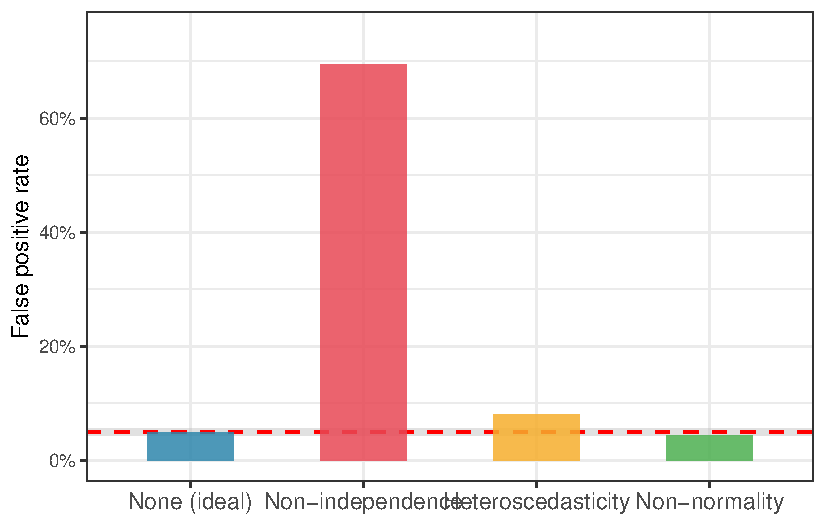
\includegraphics[width=0.9\textwidth,height=\textheight]{02b-assumptions_files/figure-pdf/fig-assumptions-comparison-plot-1.pdf}

}

\caption{\label{fig-assumptions-comparison-plot}False positive rates of
one-way ANOVA under four conditions: no violation, non-independence,
heteroscedasticity, and non-normality. The dashed red line marks the
nominal 5\% level. The shaded band is the 95\% Monte Carlo interval.
Non-independence is by far the most damaging violation; non-normality is
essentially harmless.}

\end{figure}%

\subsection{Violations do not always act
alone}\label{violations-do-not-always-act-alone}

A final and important point: assumption violations rarely occur in
isolation in real data. Non-normality and heteroscedasticity often
appear together because both can stem from the same underlying cause, a
multiplicative data-generating process, as discussed in section
\ref{sec-fix-rand}. Non-independence and heteroscedasticity can compound
each other when clusters differ not only in their means but in their
internal variability.

When multiple assumptions are simultaneously violated, the consequences
can be harder to predict than the table above suggests. The safest
strategy is not to check assumptions as a ritual box-ticking exercise
after the analysis, but to think carefully about the data-generating
process before fitting any model. Ask yourself:

\begin{itemize}
\tightlist
\item
  How were the observations collected? Is independence plausible?
\item
  Are the groups likely to differ in their variability, not just their
  means?
\item
  Is the response likely to be additive, or does the effect of the
  treatment probably scale with the baseline?
\item
  Are the groups in your study fixed choices or a random sample from a
  larger population?
\end{itemize}

These questions, answered before opening R, will protect you far more
reliably than any battery of post-hoc assumption tests.

\subsection{A decision framework}\label{a-decision-framework}

When assumptions are found to be violated, the following decision tree
provides a practical path forward:

\begin{figure}

\centering{

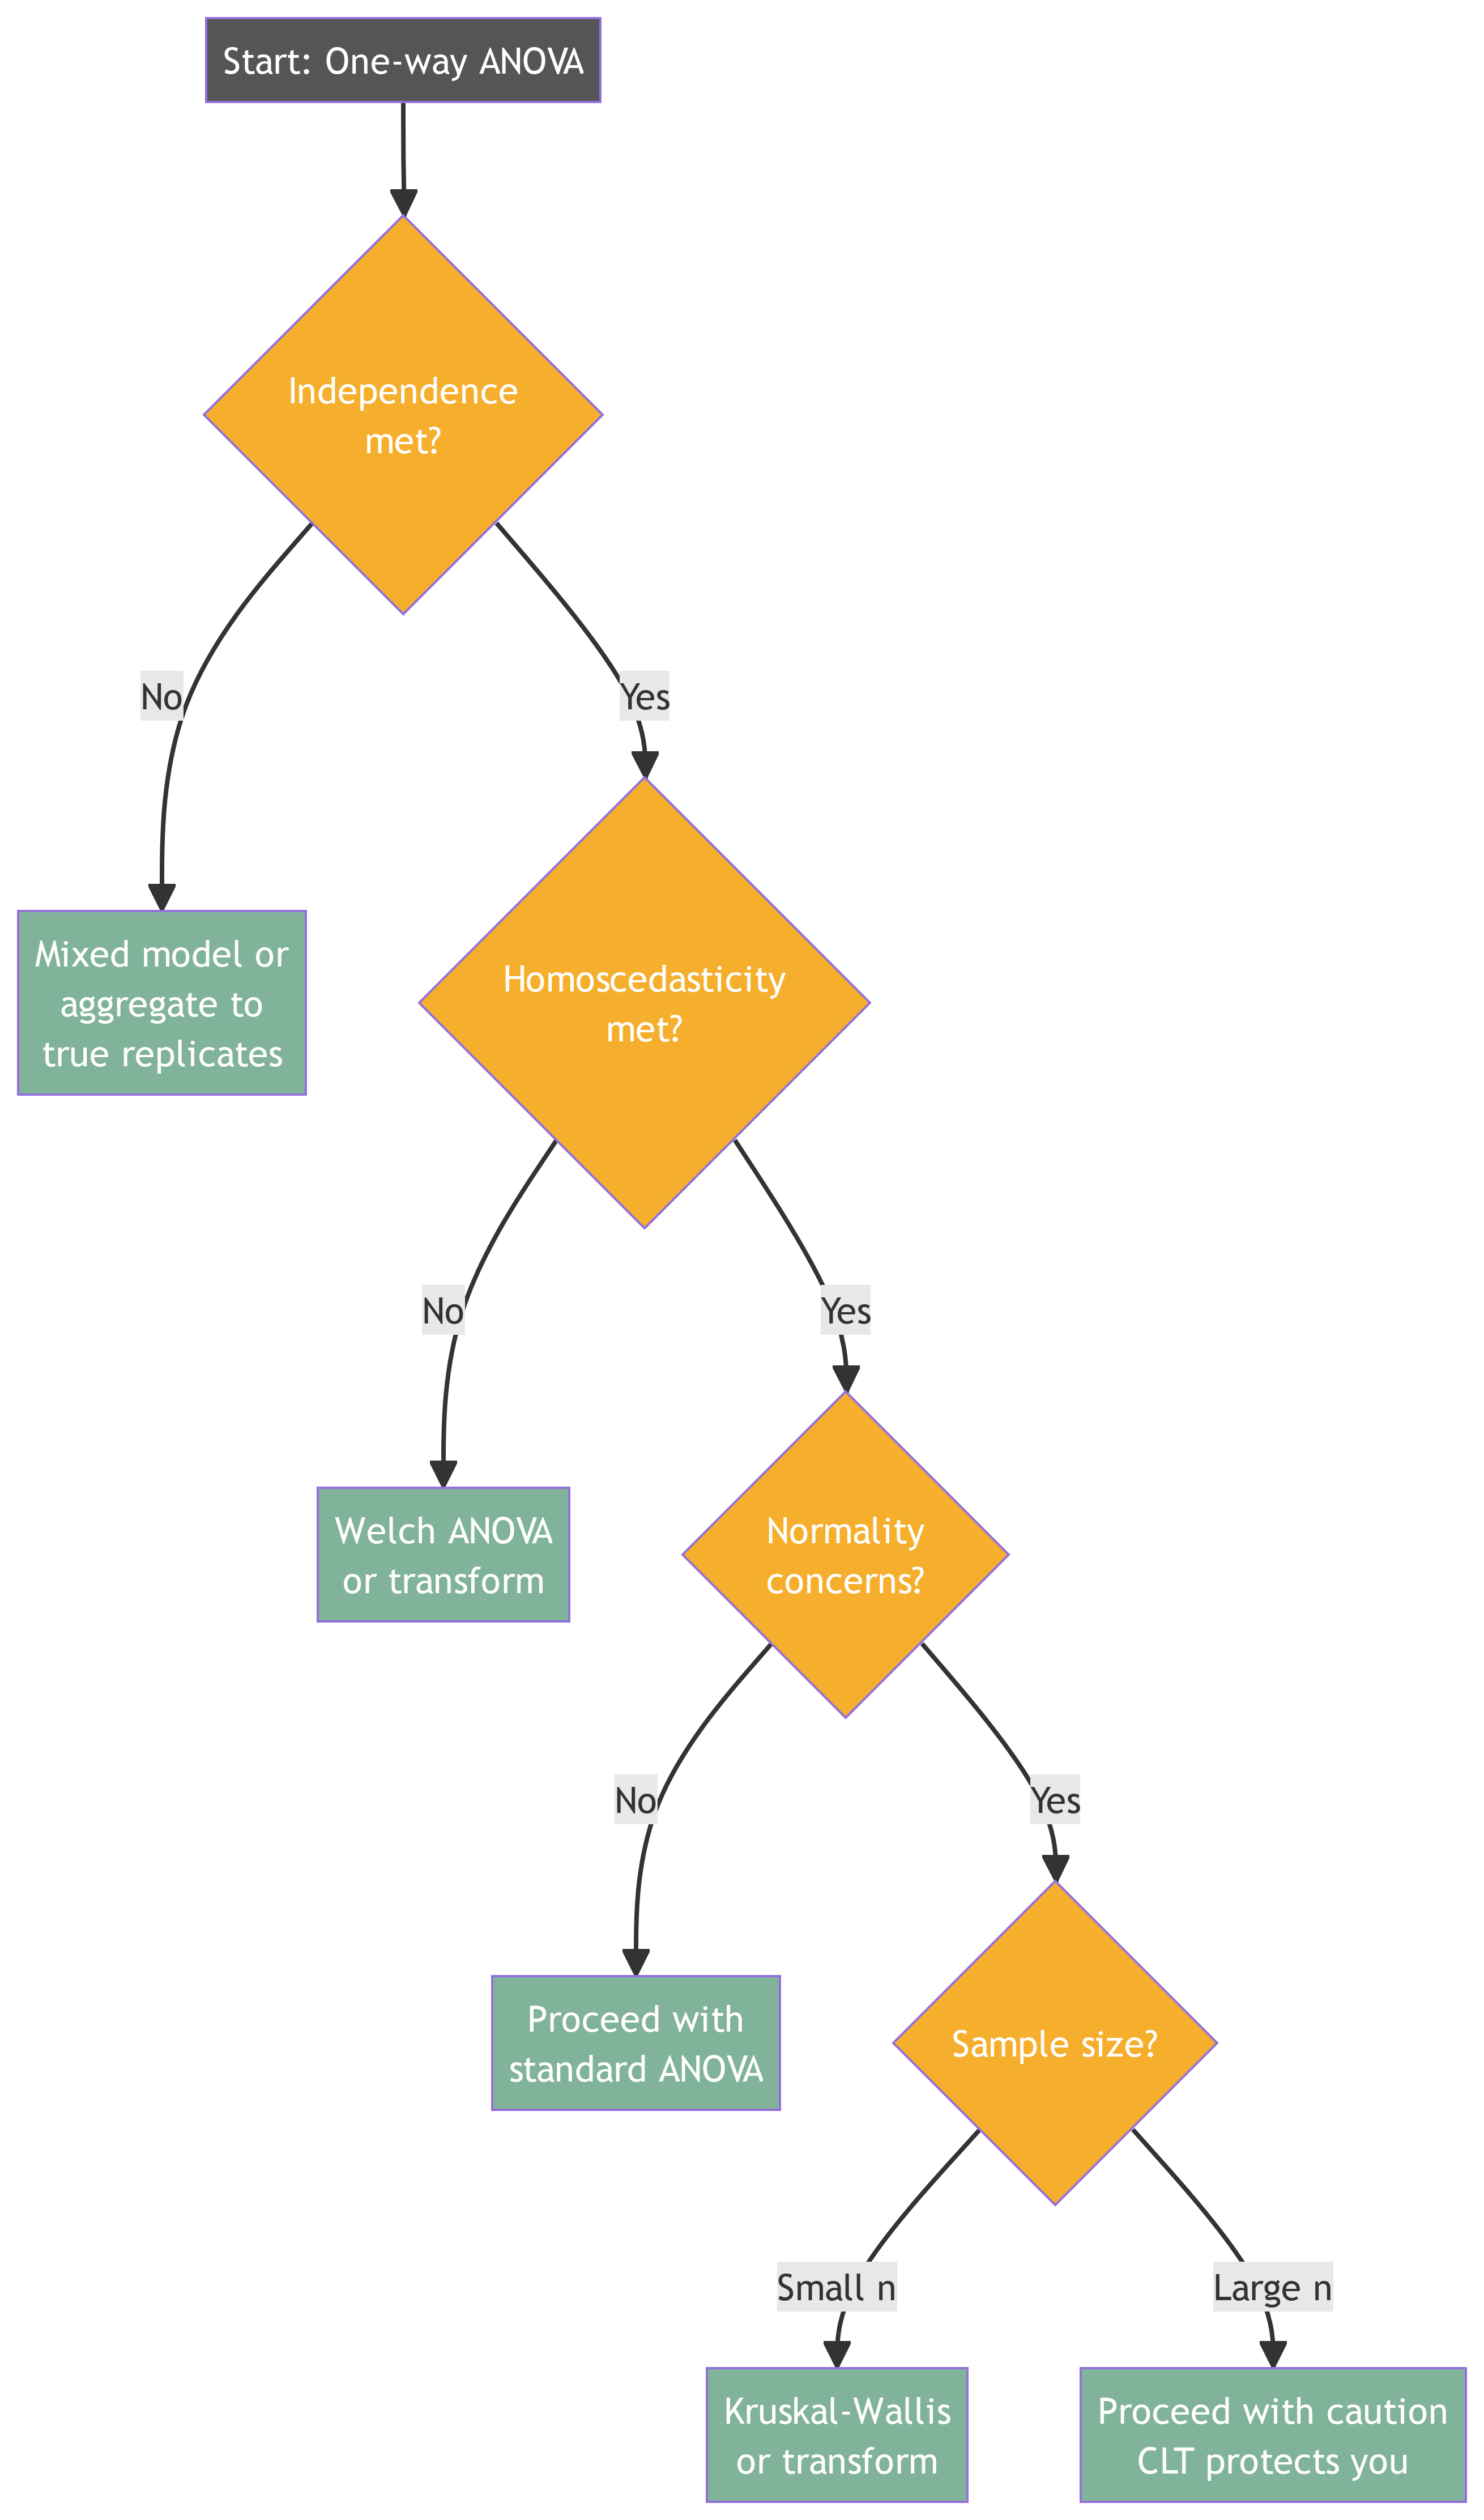
\includegraphics[width=6.82in,height=11.58in]{02b-assumptions_files/figure-latex/mermaid-figure-1.png}

}

\caption{\label{fig-assumption-decision-tree}A practical decision
framework for responding to assumption violations in one-way ANOVA.}

\end{figure}%

The central message of this chapter is simple: \textbf{not all
assumption violations are created equal.} Non-independence can
invalidate your analysis entirely. Heteroscedasticity with unequal group
sizes deserves attention and is easily addressed with Welch's ANOVA.
Non-normality, in the context of one-way ANOVA with reasonable sample
sizes, is rarely a serious problem. Understanding this hierarchy allows
you to focus your diagnostic energy where it actually matters.

\section{Checking assumptions in
practice}\label{checking-assumptions-in-practice}

The previous sections examined each assumption individually. Here we
bring everything together into a practical workflow, the sequence of
checks you should carry out every time you fit an ANOVA. The goal is not
to perform a ritual series of tests and declare the data ``clean''. It
is to understand your data well enough to know whether the conclusions
from your ANOVA are trustworthy.

\subsection{Residual diagnostics}\label{residual-diagnostics}

The single most useful thing you can do after fitting an ANOVA is to
look at the residuals. Four plots, each asking a different question,
together cover the most important assumptions.

\textbf{Plot 1: Residuals vs Fitted:} plots residuals on the \(y\)-axis
against fitted values (group means) on the \(x\)-axis. If
homoscedasticity holds, the spread of residuals should be roughly the
same across all fitted values. A fan shape, wider spread for larger
fitted values, signals heteroscedasticity. A curved pattern signals
non-additivity.

\textbf{Plot 2: Q-Q plot of residuals:} as discussed in section
\ref{sec-add-lin}, this reveals departures from normality and, more
usefully, flags outliers as isolated points flying off the diagonal
line.

\textbf{Plot 3: Scale-Location plot:} plots the square root of the
absolute residuals against fitted values. This is a more sensitive
version of Plot 1 for detecting heteroscedasticity, because it
stabilises the variance and makes trends easier to see.

\textbf{Plot 4: Residuals vs group (boxplot):} plots the residuals
separately for each group. Equal box heights confirm homoscedasticity;
outliers within groups are immediately visible; and any systematic skew
within a group suggests a transformation may be needed.

All four plots can be produced in base R with a single call, or
reconstructed in ggplot2 for more control:

\begin{Shaded}
\begin{Highlighting}[]
\FunctionTok{library}\NormalTok{(ggplot2)}
\FunctionTok{library}\NormalTok{(patchwork)}

\FunctionTok{set.seed}\NormalTok{(}\DecValTok{42}\NormalTok{)}

\CommentTok{\# Simulate clean fertiliser data for illustration}
\NormalTok{n }\OtherTok{\textless{}{-}} \DecValTok{15}
\NormalTok{group }\OtherTok{\textless{}{-}} \FunctionTok{factor}\NormalTok{(}\FunctionTok{rep}\NormalTok{(}\FunctionTok{c}\NormalTok{(}\StringTok{"Control"}\NormalTok{, }\StringTok{"Nitrogen"}\NormalTok{, }\StringTok{"Phosphorus"}\NormalTok{), }\AttributeTok{each =}\NormalTok{ n))}
\NormalTok{y }\OtherTok{\textless{}{-}} \FunctionTok{c}\NormalTok{(}
  \FunctionTok{rnorm}\NormalTok{(n, }\AttributeTok{mean =} \DecValTok{20}\NormalTok{, }\AttributeTok{sd =} \DecValTok{3}\NormalTok{),}
  \FunctionTok{rnorm}\NormalTok{(n, }\AttributeTok{mean =} \DecValTok{25}\NormalTok{, }\AttributeTok{sd =} \DecValTok{3}\NormalTok{),}
  \FunctionTok{rnorm}\NormalTok{(n, }\AttributeTok{mean =} \DecValTok{22}\NormalTok{, }\AttributeTok{sd =} \DecValTok{3}\NormalTok{)}
\NormalTok{)}
\NormalTok{df }\OtherTok{\textless{}{-}} \FunctionTok{data.frame}\NormalTok{(y, group)}
\NormalTok{fit }\OtherTok{\textless{}{-}} \FunctionTok{aov}\NormalTok{(y }\SpecialCharTok{\textasciitilde{}}\NormalTok{ group, }\AttributeTok{data =}\NormalTok{ df)}

\CommentTok{\# Extract residuals and fitted values}
\NormalTok{diag\_df }\OtherTok{\textless{}{-}} \FunctionTok{data.frame}\NormalTok{(}
  \AttributeTok{residuals =} \FunctionTok{residuals}\NormalTok{(fit),}
  \AttributeTok{fitted =} \FunctionTok{fitted}\NormalTok{(fit),}
  \AttributeTok{sqrt\_abs\_r =} \FunctionTok{sqrt}\NormalTok{(}\FunctionTok{abs}\NormalTok{(}\FunctionTok{residuals}\NormalTok{(fit))),}
  \AttributeTok{group =}\NormalTok{ group}
\NormalTok{)}

\CommentTok{\# Plot 1: Residuals vs Fitted}
\NormalTok{p1 }\OtherTok{\textless{}{-}} \FunctionTok{ggplot}\NormalTok{(diag\_df, }\FunctionTok{aes}\NormalTok{(}\AttributeTok{x =}\NormalTok{ fitted, }\AttributeTok{y =}\NormalTok{ residuals)) }\SpecialCharTok{+}
  \FunctionTok{geom\_hline}\NormalTok{(}\AttributeTok{yintercept =} \DecValTok{0}\NormalTok{, }\AttributeTok{linetype =} \StringTok{"dashed"}\NormalTok{, }\AttributeTok{colour =} \StringTok{"red"}\NormalTok{) }\SpecialCharTok{+}
  \FunctionTok{geom\_point}\NormalTok{(}\AttributeTok{colour =} \StringTok{"\#2E86AB"}\NormalTok{, }\AttributeTok{alpha =} \FloatTok{0.7}\NormalTok{) }\SpecialCharTok{+}
  \FunctionTok{geom\_smooth}\NormalTok{(}\AttributeTok{method =} \StringTok{"loess"}\NormalTok{, }\AttributeTok{se =} \ConstantTok{FALSE}\NormalTok{, }\AttributeTok{colour =} \StringTok{"\#E84855"}\NormalTok{, }\AttributeTok{linewidth =} \FloatTok{0.8}\NormalTok{) }\SpecialCharTok{+}
  \FunctionTok{labs}\NormalTok{(}\AttributeTok{title =} \StringTok{"Residuals vs Fitted"}\NormalTok{, }\AttributeTok{x =} \StringTok{"Fitted values"}\NormalTok{, }\AttributeTok{y =} \StringTok{"Residuals"}\NormalTok{) }\SpecialCharTok{+}
  \FunctionTok{theme\_bw}\NormalTok{()}

\CommentTok{\# Plot 2: Q{-}Q plot}
\NormalTok{p2 }\OtherTok{\textless{}{-}} \FunctionTok{ggplot}\NormalTok{(diag\_df, }\FunctionTok{aes}\NormalTok{(}\AttributeTok{sample =}\NormalTok{ residuals)) }\SpecialCharTok{+}
  \FunctionTok{stat\_qq}\NormalTok{(}\AttributeTok{colour =} \StringTok{"\#2E86AB"}\NormalTok{, }\AttributeTok{alpha =} \FloatTok{0.7}\NormalTok{) }\SpecialCharTok{+}
  \FunctionTok{stat\_qq\_line}\NormalTok{(}\AttributeTok{colour =} \StringTok{"\#E84855"}\NormalTok{, }\AttributeTok{linewidth =} \FloatTok{0.8}\NormalTok{) }\SpecialCharTok{+}
  \FunctionTok{labs}\NormalTok{(}\AttributeTok{title =} \StringTok{"Normal Q{-}Q"}\NormalTok{, }\AttributeTok{x =} \StringTok{"Theoretical quantiles"}\NormalTok{, }\AttributeTok{y =} \StringTok{"Sample quantiles"}\NormalTok{) }\SpecialCharTok{+}
  \FunctionTok{theme\_bw}\NormalTok{()}

\CommentTok{\# Plot 3: Scale{-}Location}
\NormalTok{p3 }\OtherTok{\textless{}{-}} \FunctionTok{ggplot}\NormalTok{(diag\_df, }\FunctionTok{aes}\NormalTok{(}\AttributeTok{x =}\NormalTok{ fitted, }\AttributeTok{y =}\NormalTok{ sqrt\_abs\_r)) }\SpecialCharTok{+}
  \FunctionTok{geom\_point}\NormalTok{(}\AttributeTok{colour =} \StringTok{"\#2E86AB"}\NormalTok{, }\AttributeTok{alpha =} \FloatTok{0.7}\NormalTok{) }\SpecialCharTok{+}
  \FunctionTok{geom\_smooth}\NormalTok{(}\AttributeTok{method =} \StringTok{"loess"}\NormalTok{, }\AttributeTok{se =} \ConstantTok{FALSE}\NormalTok{, }\AttributeTok{colour =} \StringTok{"\#E84855"}\NormalTok{, }\AttributeTok{linewidth =} \FloatTok{0.8}\NormalTok{) }\SpecialCharTok{+}
  \FunctionTok{labs}\NormalTok{(}\AttributeTok{title =} \StringTok{"Scale{-}Location"}\NormalTok{, }\AttributeTok{x =} \StringTok{"Fitted values"}\NormalTok{, }\AttributeTok{y =} \FunctionTok{expression}\NormalTok{(}\FunctionTok{sqrt}\NormalTok{(}\StringTok{"|Residuals|"}\NormalTok{))) }\SpecialCharTok{+}
  \FunctionTok{theme\_bw}\NormalTok{()}

\CommentTok{\# Plot 4: Residuals by group}
\NormalTok{p4 }\OtherTok{\textless{}{-}} \FunctionTok{ggplot}\NormalTok{(diag\_df, }\FunctionTok{aes}\NormalTok{(}\AttributeTok{x =}\NormalTok{ group, }\AttributeTok{y =}\NormalTok{ residuals, }\AttributeTok{fill =}\NormalTok{ group)) }\SpecialCharTok{+}
  \FunctionTok{geom\_hline}\NormalTok{(}\AttributeTok{yintercept =} \DecValTok{0}\NormalTok{, }\AttributeTok{linetype =} \StringTok{"dashed"}\NormalTok{, }\AttributeTok{colour =} \StringTok{"red"}\NormalTok{) }\SpecialCharTok{+}
  \FunctionTok{geom\_boxplot}\NormalTok{(}\AttributeTok{alpha =} \FloatTok{0.6}\NormalTok{, }\AttributeTok{outlier.shape =} \DecValTok{21}\NormalTok{) }\SpecialCharTok{+}
  \FunctionTok{scale\_fill\_manual}\NormalTok{(}\AttributeTok{values =} \FunctionTok{c}\NormalTok{(}\StringTok{"\#2E86AB"}\NormalTok{, }\StringTok{"\#F6AE2D"}\NormalTok{, }\StringTok{"\#E84855"}\NormalTok{)) }\SpecialCharTok{+}
  \FunctionTok{labs}\NormalTok{(}\AttributeTok{title =} \StringTok{"Residuals by Group"}\NormalTok{, }\AttributeTok{x =} \ConstantTok{NULL}\NormalTok{, }\AttributeTok{y =} \StringTok{"Residuals"}\NormalTok{) }\SpecialCharTok{+}
  \FunctionTok{theme\_bw}\NormalTok{() }\SpecialCharTok{+}
  \FunctionTok{theme}\NormalTok{(}\AttributeTok{legend.position =} \StringTok{"none"}\NormalTok{)}

\NormalTok{(p1 }\SpecialCharTok{+}\NormalTok{ p2) }\SpecialCharTok{/}\NormalTok{ (p3 }\SpecialCharTok{+}\NormalTok{ p4)}
\end{Highlighting}
\end{Shaded}

\begin{figure}[H]

\centering{

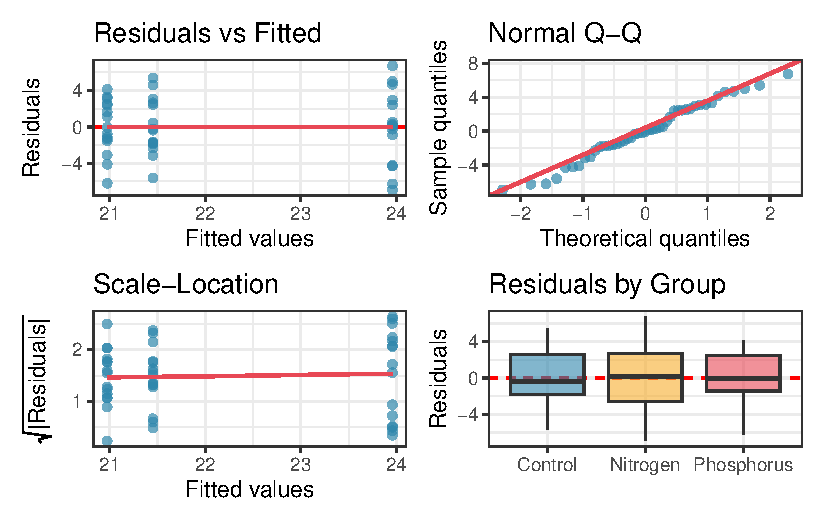
\includegraphics[width=0.9\textwidth,height=\textheight]{02b-assumptions_files/figure-pdf/fig-residual-diagnostics-1.pdf}

}

\caption{\label{fig-residual-diagnostics}Four residual diagnostic plots
for a one-way ANOVA fitted to the fertiliser data. Top left: residuals
vs fitted values --- roughly equal spread across groups confirms
homoscedasticity. Top right: Q-Q plot, points close to the line confirm
approximate normality. Bottom left: scale-location plot, a flat trend
confirms homoscedasticity. Bottom right: residuals by group, box heights
are similar and no extreme outliers are present.}

\end{figure}%

These four plots together give you a comprehensive picture of whether
the assumptions are reasonably met. Learn to read them before reaching
for any formal test.

\subsection{The Shapiro-Wilk trap}\label{the-shapiro-wilk-trap}

The Shapiro-Wilk test is the most commonly used formal test of
normality. It tests the null hypothesis that the residuals were drawn
from a normal distribution, returning a \(p\)-value that students often
use as a binary gate: \(p > 0.05\) means ``normality confirmed,
proceed''; \(p < 0.05\) means ``normality violated, stop''.

This is a trap, and it fails in both directions simultaneously.

\textbf{With small samples}, the Shapiro-Wilk test has very low power.
It will return \(p > 0.05\), apparently confirming normality, even when
the residuals are substantially non-normal, simply because there are too
few observations to detect the departure. The test tells you nothing
useful precisely when sample size is small and normality matters most.

\textbf{With large samples}, the Shapiro-Wilk test becomes
hypersensitive. It will return \(p < 0.05\), apparently rejecting
normality, for trivially small deviations that have no practical
consequence for the \(F\) test whatsoever. The larger your sample, the
more likely you are to get a significant result even when your residuals
are, for all practical purposes, perfectly normal.

The simulation below demonstrates both failure modes:

\begin{Shaded}
\begin{Highlighting}[]
\FunctionTok{set.seed}\NormalTok{(}\DecValTok{42}\NormalTok{)}
\NormalTok{n\_sim }\OtherTok{\textless{}{-}} \DecValTok{2000}

\CommentTok{\# Small sample trap: low power to detect real non{-}normality}
\NormalTok{p\_small }\OtherTok{\textless{}{-}} \FunctionTok{replicate}\NormalTok{(n\_sim, \{}
  \CommentTok{\# Clearly non{-}normal: exponential residuals}
\NormalTok{  y     }\OtherTok{\textless{}{-}} \FunctionTok{rexp}\NormalTok{(}\DecValTok{3} \SpecialCharTok{*} \DecValTok{5}\NormalTok{, }\AttributeTok{rate =} \DecValTok{1}\NormalTok{)}
\NormalTok{  group }\OtherTok{\textless{}{-}} \FunctionTok{factor}\NormalTok{(}\FunctionTok{rep}\NormalTok{(letters[}\DecValTok{1}\SpecialCharTok{:}\DecValTok{3}\NormalTok{], }\AttributeTok{each =} \DecValTok{5}\NormalTok{))}
\NormalTok{  fit   }\OtherTok{\textless{}{-}} \FunctionTok{aov}\NormalTok{(y }\SpecialCharTok{\textasciitilde{}}\NormalTok{ group)}
  \FunctionTok{shapiro.test}\NormalTok{(}\FunctionTok{residuals}\NormalTok{(fit))}\SpecialCharTok{$}\NormalTok{p.value}
\NormalTok{\})}

\CommentTok{\# Large sample trap: detects trivial non{-}normality}
\NormalTok{p\_large }\OtherTok{\textless{}{-}} \FunctionTok{replicate}\NormalTok{(n\_sim, \{}
  \CommentTok{\# Nearly normal: just a tiny skew added}
\NormalTok{  y     }\OtherTok{\textless{}{-}} \FunctionTok{rnorm}\NormalTok{(}\DecValTok{3} \SpecialCharTok{*} \DecValTok{200}\NormalTok{) }\SpecialCharTok{+} \FloatTok{0.05} \SpecialCharTok{*} \FunctionTok{rexp}\NormalTok{(}\DecValTok{3} \SpecialCharTok{*} \DecValTok{200}\NormalTok{)}
\NormalTok{  group }\OtherTok{\textless{}{-}} \FunctionTok{factor}\NormalTok{(}\FunctionTok{rep}\NormalTok{(letters[}\DecValTok{1}\SpecialCharTok{:}\DecValTok{3}\NormalTok{], }\AttributeTok{each =} \DecValTok{200}\NormalTok{))}
\NormalTok{  fit   }\OtherTok{\textless{}{-}} \FunctionTok{aov}\NormalTok{(y }\SpecialCharTok{\textasciitilde{}}\NormalTok{ group)}
  \FunctionTok{shapiro.test}\NormalTok{(}\FunctionTok{residuals}\NormalTok{(fit))}\SpecialCharTok{$}\NormalTok{p.value}
\NormalTok{\})}

\FunctionTok{cat}\NormalTok{(}
  \StringTok{"Small n: proportion of tests detecting non{-}normality:"}\NormalTok{,}
  \FunctionTok{round}\NormalTok{(}\FunctionTok{mean}\NormalTok{(p\_small }\SpecialCharTok{\textless{}} \FloatTok{0.05}\NormalTok{), }\DecValTok{3}\NormalTok{), }
  \StringTok{"}\SpecialCharTok{\textbackslash{}n}\StringTok{Large n: proportion of tests rejecting near{-}normal data:"}\NormalTok{,}
  \FunctionTok{round}\NormalTok{(}\FunctionTok{mean}\NormalTok{(p\_large }\SpecialCharTok{\textless{}} \FloatTok{0.05}\NormalTok{), }\DecValTok{3}\NormalTok{), }\StringTok{"}\SpecialCharTok{\textbackslash{}n}\StringTok{"}
\NormalTok{  )}
\end{Highlighting}
\end{Shaded}

\begin{verbatim}
#> Small n: proportion of tests detecting non-normality: 0.368 
#> Large n: proportion of tests rejecting near-normal data: 0.059
\end{verbatim}

\begin{Shaded}
\begin{Highlighting}[]
\CommentTok{\# Plot}
\NormalTok{trap\_df }\OtherTok{\textless{}{-}} \FunctionTok{data.frame}\NormalTok{(}
  \AttributeTok{p\_value  =} \FunctionTok{c}\NormalTok{(p\_small, p\_large),}
  \AttributeTok{scenario =} \FunctionTok{rep}\NormalTok{(}\FunctionTok{c}\NormalTok{(}\StringTok{"Small n (n=5 per group)}\SpecialCharTok{\textbackslash{}n}\StringTok{Clearly non{-}normal data"}\NormalTok{,}
                   \StringTok{"Large n (n=200 per group)}\SpecialCharTok{\textbackslash{}n}\StringTok{Nearly normal data"}\NormalTok{),}
                 \AttributeTok{each =}\NormalTok{ n\_sim)}
\NormalTok{)}

\FunctionTok{ggplot}\NormalTok{(trap\_df, }\FunctionTok{aes}\NormalTok{(}\AttributeTok{x =}\NormalTok{ p\_value, }\AttributeTok{fill =}\NormalTok{ scenario)) }\SpecialCharTok{+}
  \FunctionTok{geom\_histogram}\NormalTok{(}\AttributeTok{binwidth =} \FloatTok{0.05}\NormalTok{, }\AttributeTok{boundary =} \DecValTok{0}\NormalTok{, }\AttributeTok{colour =} \StringTok{"white"}\NormalTok{) }\SpecialCharTok{+}
  \FunctionTok{geom\_vline}\NormalTok{(}\AttributeTok{xintercept =} \FloatTok{0.05}\NormalTok{, }\AttributeTok{linetype =} \StringTok{"dashed"}\NormalTok{, }\AttributeTok{colour =} \StringTok{"red"}\NormalTok{, }\AttributeTok{linewidth =} \FloatTok{0.8}\NormalTok{) }\SpecialCharTok{+}
  \FunctionTok{facet\_wrap}\NormalTok{(}\SpecialCharTok{\textasciitilde{}}\NormalTok{ scenario, }\AttributeTok{ncol =} \DecValTok{2}\NormalTok{) }\SpecialCharTok{+}
  \FunctionTok{scale\_fill\_manual}\NormalTok{(}\AttributeTok{values =} \FunctionTok{c}\NormalTok{(}\StringTok{"\#2E86AB"}\NormalTok{, }\StringTok{"\#E84855"}\NormalTok{)) }\SpecialCharTok{+}
  \FunctionTok{labs}\NormalTok{(}\AttributeTok{x =} \StringTok{"Shapiro{-}Wilk p{-}value"}\NormalTok{, }\AttributeTok{y =} \StringTok{"Count"}\NormalTok{) }\SpecialCharTok{+}
  \FunctionTok{theme\_bw}\NormalTok{() }\SpecialCharTok{+}
  \FunctionTok{theme}\NormalTok{(}\AttributeTok{legend.position =} \StringTok{"none"}\NormalTok{)}
\end{Highlighting}
\end{Shaded}

\begin{figure}[H]

\centering{

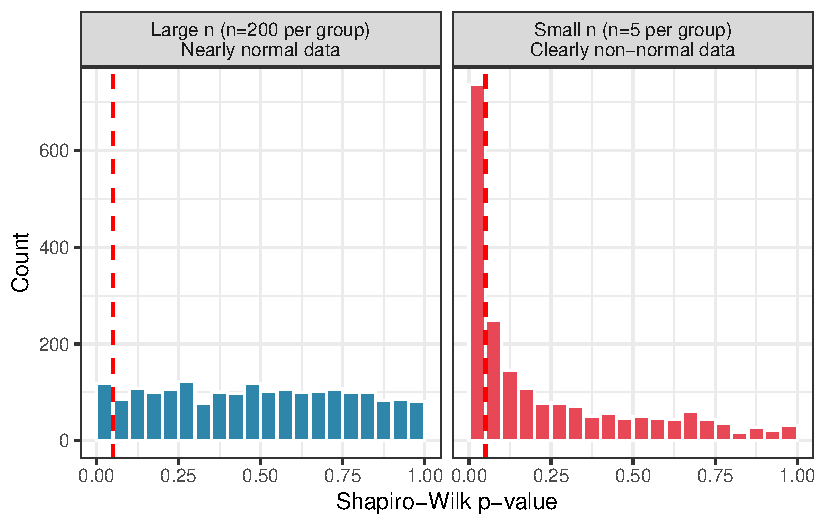
\includegraphics[width=0.9\textwidth,height=\textheight]{02b-assumptions_files/figure-pdf/fig-shapiro-trap-1.pdf}

}

\caption{\label{fig-shapiro-trap}The Shapiro-Wilk trap illustrated.
Left: with small samples (n = 5 per group), the test fails to detect
clear non-normality, returning p \textgreater{} 0.05 in the majority of
cases. Right: with large samples (n = 200 per group), the test rejects
normality almost universally, even for data generated from an exactly
normal distribution with only a trivial added skew.}

\end{figure}%

The conclusion is not that the Shapiro-Wilk test is useless, it can be a
helpful supplement to a Q-Q plot. The conclusion is that its \(p\)-value
should never be used as a binary decision rule. Use it as one piece of
evidence among several, always in conjunction with the Q-Q plot, and
always with awareness of your sample size.

\subsection{Levene's, Bartlett's, and why formal tests are not
enough}\label{levenes-bartletts-and-why-formal-tests-are-not-enough}

Two formal tests are commonly used to check homoscedasticity.

\textbf{Bartlett's test} is sensitive to departures from normality as
well as to unequal variances. If your residuals are non-normal,
Bartlett's test may reject the null hypothesis of equal variances even
when the variances are in fact equal, it is detecting the non-normality,
not the heteroscedasticity. For this reason, Bartlett's test \emph{is
generally not recommended in practice} unless you are confident that the
residuals are close to normal.

\textbf{Levene's test} is more robust. It tests for equal variances by
running an ANOVA not on the raw residuals but on the absolute deviations
from each group median, making it much less sensitive to non-normality.
\emph{It is the preferred formal test for homoscedasticity in most
situations.}

\begin{Shaded}
\begin{Highlighting}[]
\FunctionTok{library}\NormalTok{(car)}

\CommentTok{\# Bartlett\textquotesingle{}s test (sensitive to non{-}normality)}
\FunctionTok{bartlett.test}\NormalTok{(y }\SpecialCharTok{\textasciitilde{}}\NormalTok{ group, }\AttributeTok{data =}\NormalTok{ df)}
\end{Highlighting}
\end{Shaded}

\begin{verbatim}
#> 
#>  Bartlett test of homogeneity of variances
#> 
#> data:  y by group
#> Bartlett's K-squared = 1.661, df = 2, p-value = 0.4358
\end{verbatim}

\begin{Shaded}
\begin{Highlighting}[]
\CommentTok{\# Levene\textquotesingle{}s test (robust to non{-}normality)}
\FunctionTok{leveneTest}\NormalTok{(y }\SpecialCharTok{\textasciitilde{}}\NormalTok{ group, }\AttributeTok{data =}\NormalTok{ df)}
\end{Highlighting}
\end{Shaded}

\begin{verbatim}
#> Levene's Test for Homogeneity of Variance (center = median)
#>       Df F value Pr(>F)
#> group  2  0.4118 0.6651
#>       42
\end{verbatim}

However, formal tests for homoscedasticity suffer from exactly the same
sample size problem as the Shapiro-Wilk test. The simulation below
demonstrates this for Levene's test.

\begin{Shaded}
\begin{Highlighting}[]
\FunctionTok{set.seed}\NormalTok{(}\DecValTok{42}\NormalTok{)}

\CommentTok{\# Small n: misses real heteroscedasticity}
\NormalTok{p\_lev\_small }\OtherTok{\textless{}{-}} \FunctionTok{replicate}\NormalTok{(n\_sim, \{}
\NormalTok{  y }\OtherTok{\textless{}{-}} \FunctionTok{c}\NormalTok{(}\FunctionTok{rnorm}\NormalTok{(}\DecValTok{5}\NormalTok{, }\AttributeTok{sd =} \DecValTok{1}\NormalTok{), }\FunctionTok{rnorm}\NormalTok{(}\DecValTok{5}\NormalTok{, }\AttributeTok{sd =} \DecValTok{3}\NormalTok{), }\FunctionTok{rnorm}\NormalTok{(}\DecValTok{5}\NormalTok{, }\AttributeTok{sd =} \DecValTok{9}\NormalTok{))}
\NormalTok{  group }\OtherTok{\textless{}{-}} \FunctionTok{factor}\NormalTok{(}\FunctionTok{rep}\NormalTok{(letters[}\DecValTok{1}\SpecialCharTok{:}\DecValTok{3}\NormalTok{], }\AttributeTok{each =} \DecValTok{5}\NormalTok{))}
  \FunctionTok{leveneTest}\NormalTok{(y }\SpecialCharTok{\textasciitilde{}}\NormalTok{ group)}\SpecialCharTok{$}\StringTok{\textasciigrave{}}\AttributeTok{Pr(\textgreater{}F)}\StringTok{\textasciigrave{}}\NormalTok{[}\DecValTok{1}\NormalTok{]}
\NormalTok{\})}

\CommentTok{\# Large n: detects trivial heteroscedasticity}
\NormalTok{p\_lev\_large }\OtherTok{\textless{}{-}} \FunctionTok{replicate}\NormalTok{(n\_sim, \{}
\NormalTok{  y }\OtherTok{\textless{}{-}} \FunctionTok{c}\NormalTok{(}\FunctionTok{rnorm}\NormalTok{(}\DecValTok{200}\NormalTok{, }\AttributeTok{sd =} \FloatTok{1.0}\NormalTok{), }\FunctionTok{rnorm}\NormalTok{(}\DecValTok{200}\NormalTok{, }\AttributeTok{sd =} \FloatTok{1.1}\NormalTok{), }\FunctionTok{rnorm}\NormalTok{(}\DecValTok{200}\NormalTok{, }\AttributeTok{sd =} \FloatTok{1.2}\NormalTok{))}
\NormalTok{  group }\OtherTok{\textless{}{-}} \FunctionTok{factor}\NormalTok{(}\FunctionTok{rep}\NormalTok{(letters[}\DecValTok{1}\SpecialCharTok{:}\DecValTok{3}\NormalTok{], }\AttributeTok{each =} \DecValTok{200}\NormalTok{))}
  \FunctionTok{leveneTest}\NormalTok{(y }\SpecialCharTok{\textasciitilde{}}\NormalTok{ group)}\SpecialCharTok{$}\StringTok{\textasciigrave{}}\AttributeTok{Pr(\textgreater{}F)}\StringTok{\textasciigrave{}}\NormalTok{[}\DecValTok{1}\NormalTok{]}
\NormalTok{\})}

\FunctionTok{cat}\NormalTok{(}
  \StringTok{"Small n: detecting large variance differences (sd = 1, 3, 9):"}\NormalTok{,}
  \FunctionTok{round}\NormalTok{(}\FunctionTok{mean}\NormalTok{(p\_lev\_small }\SpecialCharTok{\textless{}} \FloatTok{0.05}\NormalTok{), }\DecValTok{3}\NormalTok{),}
  \StringTok{"}\SpecialCharTok{\textbackslash{}n}\StringTok{Large n: flagging trivial variance differences (sd = 1, 1.1, 1.2):"}\NormalTok{,}
  \FunctionTok{round}\NormalTok{(}\FunctionTok{mean}\NormalTok{(p\_lev\_large }\SpecialCharTok{\textless{}} \FloatTok{0.05}\NormalTok{), }\DecValTok{3}\NormalTok{), }\StringTok{"}\SpecialCharTok{\textbackslash{}n}\StringTok{"}
\NormalTok{  )}
\end{Highlighting}
\end{Shaded}

\begin{verbatim}
#> Small n: detecting large variance differences (sd = 1, 3, 9): 0.3 
#> Large n: flagging trivial variance differences (sd = 1, 1.1, 1.2): 0.552
\end{verbatim}

The practical implication is the same as for the Shapiro-Wilk test:
formal tests of assumptions should inform your judgement, not replace
it. A non-significant Levene's test with \(n = 5\) per group tells you
almost nothing. A significant Levene's test with \(n = 200\) per group
may be flagging a difference in variance so small that Welch's ANOVA and
standard ANOVA would give virtually identical results.

The best habit is to always look at the residual boxplot by group first.
If one box is three or four times taller than the others, the variances
are unequal in a practically meaningful way, regardless of what Levene's
test says. If the boxes are roughly similar in height, the variances are
probably close enough, again, regardless of what Levene's test says.

\subsection{Building a diagnostic workflow in
R}\label{building-a-diagnostic-workflow-in-r}

Here I provide a complete, reusable diagnostic function that produces
all the key plots and tests in a single call. You can write this once at
the top of your analysis script and call it every time you fit an ANOVA.

\begin{Shaded}
\begin{Highlighting}[]
\NormalTok{anova\_diagnostics }\OtherTok{\textless{}{-}} \ControlFlowTok{function}\NormalTok{(fit, data) \{}
  \CommentTok{\# required packages}
  \ControlFlowTok{if}\NormalTok{ (}\SpecialCharTok{!}\FunctionTok{requireNamespace}\NormalTok{(}\StringTok{"ggplot2"}\NormalTok{, }\AttributeTok{quietly =} \ConstantTok{TRUE}\NormalTok{)) \{}
    \FunctionTok{stop}\NormalTok{(}\StringTok{"anova\_diagnostics needs ggplot2 package."}\NormalTok{)}
\NormalTok{  \}}
  
  \ControlFlowTok{if}\NormalTok{ (}\SpecialCharTok{!}\FunctionTok{requireNamespace}\NormalTok{(}\StringTok{"patchwork"}\NormalTok{, }\AttributeTok{quietly =} \ConstantTok{TRUE}\NormalTok{)) \{}
    \FunctionTok{stop}\NormalTok{(}\StringTok{"anova\_diagnostics needs patchwork package."}\NormalTok{)}
\NormalTok{  \}}
  
  \ControlFlowTok{if}\NormalTok{ (}\SpecialCharTok{!}\FunctionTok{requireNamespace}\NormalTok{(}\StringTok{"car"}\NormalTok{, }\AttributeTok{quietly =} \ConstantTok{TRUE}\NormalTok{)) \{}
    \FunctionTok{stop}\NormalTok{(}\StringTok{"anova\_diagnostics needs car package."}\NormalTok{)}
\NormalTok{  \}}
  
  \CommentTok{\# extract residuals and fitted values}
\NormalTok{  res }\OtherTok{\textless{}{-}} \FunctionTok{residuals}\NormalTok{(fit)}
\NormalTok{  fitt }\OtherTok{\textless{}{-}} \FunctionTok{fitted}\NormalTok{(fit)}
  
  \CommentTok{\# robustly extract the first grouping variable from the formula}
  \CommentTok{\# works for both one{-}way (y \textasciitilde{} A) and two{-}way (y \textasciitilde{} A * B) formulas}
\NormalTok{  rhs\_vars }\OtherTok{\textless{}{-}} \FunctionTok{all.vars}\NormalTok{(}\FunctionTok{formula}\NormalTok{(fit)[[}\DecValTok{3}\NormalTok{]])}
\NormalTok{  grp }\OtherTok{\textless{}{-}} \FunctionTok{factor}\NormalTok{(data[[rhs\_vars[}\DecValTok{1}\NormalTok{]]])}
  
\NormalTok{  diag\_df }\OtherTok{\textless{}{-}} \FunctionTok{data.frame}\NormalTok{(}
    \AttributeTok{residuals =}\NormalTok{ res,}
    \AttributeTok{fitted =}\NormalTok{ fitt,}
    \AttributeTok{sqrt\_abs\_r =} \FunctionTok{sqrt}\NormalTok{(}\FunctionTok{abs}\NormalTok{(res)),}
    \AttributeTok{group =}\NormalTok{ grp}
\NormalTok{  )}
  
  \CommentTok{\# plot 1: residuals vs fitted}
\NormalTok{  p1 }\OtherTok{\textless{}{-}} \FunctionTok{ggplot}\NormalTok{(diag\_df, }\FunctionTok{aes}\NormalTok{(}\AttributeTok{x =}\NormalTok{ fitted, }\AttributeTok{y =}\NormalTok{ residuals)) }\SpecialCharTok{+}
    \FunctionTok{geom\_hline}\NormalTok{(}\AttributeTok{yintercept =} \DecValTok{0}\NormalTok{, }\AttributeTok{linetype =} \StringTok{"dashed"}\NormalTok{, }\AttributeTok{colour =} \StringTok{"red"}\NormalTok{) }\SpecialCharTok{+}
    \FunctionTok{geom\_point}\NormalTok{(}\AttributeTok{colour =} \StringTok{"\#2E86AB"}\NormalTok{, }\AttributeTok{alpha =} \FloatTok{0.7}\NormalTok{) }\SpecialCharTok{+}
    \FunctionTok{geom\_smooth}\NormalTok{(}\AttributeTok{method =} \StringTok{"loess"}\NormalTok{, }\AttributeTok{se =} \ConstantTok{FALSE}\NormalTok{, }\AttributeTok{colour =} \StringTok{"\#E84855"}\NormalTok{, }\AttributeTok{linewidth =} \FloatTok{0.8}\NormalTok{) }\SpecialCharTok{+}
    \FunctionTok{labs}\NormalTok{(}\AttributeTok{title =} \StringTok{"Residuals vs Fitted"}\NormalTok{, }\AttributeTok{x =} \StringTok{"Fitted values"}\NormalTok{, }\AttributeTok{y =} \StringTok{"Residuals"}\NormalTok{) }\SpecialCharTok{+}
    \FunctionTok{theme\_bw}\NormalTok{()}
  
  \CommentTok{\# plot 2: Q{-}Q plot}
\NormalTok{  p2 }\OtherTok{\textless{}{-}} \FunctionTok{ggplot}\NormalTok{(diag\_df, }\FunctionTok{aes}\NormalTok{(}\AttributeTok{sample =}\NormalTok{ residuals)) }\SpecialCharTok{+}
    \FunctionTok{stat\_qq}\NormalTok{(}\AttributeTok{colour =} \StringTok{"\#2E86AB"}\NormalTok{, }\AttributeTok{alpha =} \FloatTok{0.7}\NormalTok{) }\SpecialCharTok{+}
    \FunctionTok{stat\_qq\_line}\NormalTok{(}\AttributeTok{colour =} \StringTok{"\#E84855"}\NormalTok{, }\AttributeTok{linewidth =} \FloatTok{0.8}\NormalTok{) }\SpecialCharTok{+}
    \FunctionTok{labs}\NormalTok{(}\AttributeTok{title =} \StringTok{"Normal Q{-}Q"}\NormalTok{, }\AttributeTok{x =} \StringTok{"Theoretical quantiles"}\NormalTok{, }\AttributeTok{y =} \StringTok{"Sample quantiles"}\NormalTok{) }\SpecialCharTok{+}
    \FunctionTok{theme\_bw}\NormalTok{()}
  
  \CommentTok{\# plot 3: Scale{-}Location}
\NormalTok{  p3 }\OtherTok{\textless{}{-}} \FunctionTok{ggplot}\NormalTok{(diag\_df, }\FunctionTok{aes}\NormalTok{(}\AttributeTok{x =}\NormalTok{ fitted, }\AttributeTok{y =}\NormalTok{ sqrt\_abs\_r)) }\SpecialCharTok{+}
    \FunctionTok{geom\_point}\NormalTok{(}\AttributeTok{colour =} \StringTok{"\#2E86AB"}\NormalTok{, }\AttributeTok{alpha =} \FloatTok{0.7}\NormalTok{) }\SpecialCharTok{+}
    \FunctionTok{geom\_smooth}\NormalTok{(}\AttributeTok{method =} \StringTok{"loess"}\NormalTok{, }\AttributeTok{se =} \ConstantTok{FALSE}\NormalTok{, }\AttributeTok{colour =} \StringTok{"\#E84855"}\NormalTok{, }\AttributeTok{linewidth =} \FloatTok{0.8}\NormalTok{) }\SpecialCharTok{+}
    \FunctionTok{labs}\NormalTok{(}\AttributeTok{title =} \StringTok{"Scale{-}Location"}\NormalTok{, }\AttributeTok{x =} \StringTok{"Fitted values"}\NormalTok{, }\AttributeTok{y =} \FunctionTok{expression}\NormalTok{(}\FunctionTok{sqrt}\NormalTok{(}\StringTok{"|Residuals|"}\NormalTok{))) }\SpecialCharTok{+}
    \FunctionTok{theme\_bw}\NormalTok{()}
  
  \CommentTok{\# plot 4: Residuals by first grouping variable}
\NormalTok{  p4 }\OtherTok{\textless{}{-}} \FunctionTok{ggplot}\NormalTok{(diag\_df, }\FunctionTok{aes}\NormalTok{(}\AttributeTok{x =}\NormalTok{ group, }\AttributeTok{y =}\NormalTok{ residuals, }\AttributeTok{fill =}\NormalTok{ group)) }\SpecialCharTok{+}
    \FunctionTok{geom\_hline}\NormalTok{(}\AttributeTok{yintercept =} \DecValTok{0}\NormalTok{, }\AttributeTok{linetype =} \StringTok{"dashed"}\NormalTok{, }\AttributeTok{colour =} \StringTok{"red"}\NormalTok{) }\SpecialCharTok{+}
    \FunctionTok{geom\_boxplot}\NormalTok{(}\AttributeTok{alpha =} \FloatTok{0.6}\NormalTok{, }\AttributeTok{outlier.shape =} \DecValTok{21}\NormalTok{) }\SpecialCharTok{+}
    \FunctionTok{labs}\NormalTok{(}\AttributeTok{title   =} \FunctionTok{paste}\NormalTok{(}\StringTok{"Residuals by"}\NormalTok{, rhs\_vars[}\DecValTok{1}\NormalTok{]), }\AttributeTok{x =} \ConstantTok{NULL}\NormalTok{, }\AttributeTok{y =} \StringTok{"Residuals"}\NormalTok{) }\SpecialCharTok{+}
    \FunctionTok{theme\_bw}\NormalTok{() }\SpecialCharTok{+}
    \FunctionTok{theme}\NormalTok{(}\AttributeTok{legend.position =} \StringTok{"none"}\NormalTok{)}
  
  \FunctionTok{print}\NormalTok{((p1 }\SpecialCharTok{+}\NormalTok{ p2) }\SpecialCharTok{/}\NormalTok{ (p3 }\SpecialCharTok{+}\NormalTok{ p4))}
  
  \CommentTok{\# Formal tests}
  \FunctionTok{cat}\NormalTok{(}\StringTok{"}\SpecialCharTok{\textbackslash{}n}\StringTok{{-}{-}{-} Shapiro{-}Wilk test (normality of residuals) {-}{-}{-}}\SpecialCharTok{\textbackslash{}n}\StringTok{"}\NormalTok{)}
  \FunctionTok{print}\NormalTok{(}\FunctionTok{shapiro.test}\NormalTok{(res))}
  
  \FunctionTok{cat}\NormalTok{(}\StringTok{"}\SpecialCharTok{\textbackslash{}n}\StringTok{{-}{-}{-} Levene\textquotesingle{}s test (homogeneity of variance) {-}{-}{-}}\SpecialCharTok{\textbackslash{}n}\StringTok{"}\NormalTok{)}
  \FunctionTok{print}\NormalTok{(}\FunctionTok{leveneTest}\NormalTok{(res }\SpecialCharTok{\textasciitilde{}}\NormalTok{ grp))}
  
  \CommentTok{\# Summary guidance}
\NormalTok{  sw\_p }\OtherTok{\textless{}{-}} \FunctionTok{shapiro.test}\NormalTok{(res)}\SpecialCharTok{$}\NormalTok{p.value}
\NormalTok{  lev\_p }\OtherTok{\textless{}{-}} \FunctionTok{leveneTest}\NormalTok{(res }\SpecialCharTok{\textasciitilde{}}\NormalTok{ grp)}\SpecialCharTok{$}\StringTok{\textasciigrave{}}\AttributeTok{Pr(\textgreater{}F)}\StringTok{\textasciigrave{}}\NormalTok{[}\DecValTok{1}\NormalTok{]}
\NormalTok{  n\_grp }\OtherTok{\textless{}{-}} \FunctionTok{min}\NormalTok{(}\FunctionTok{table}\NormalTok{(grp))}
  
  \FunctionTok{cat}\NormalTok{(}\StringTok{"}\SpecialCharTok{\textbackslash{}n}\StringTok{{-}{-}{-} Diagnostic summary {-}{-}{-}}\SpecialCharTok{\textbackslash{}n}\StringTok{"}\NormalTok{)}
  \FunctionTok{cat}\NormalTok{(}\StringTok{"Sample size (smallest group):"}\NormalTok{, n\_grp, }\StringTok{"}\SpecialCharTok{\textbackslash{}n}\StringTok{"}\NormalTok{)}
  
  \ControlFlowTok{if}\NormalTok{ (n\_grp }\SpecialCharTok{\textless{}} \DecValTok{10}\NormalTok{) \{}
    \FunctionTok{cat}\NormalTok{(}\StringTok{"  Note: formal tests have low power with small samples.}\SpecialCharTok{\textbackslash{}n}\StringTok{"}\NormalTok{,}
        \StringTok{"  Prioritise plots over p{-}values.}\SpecialCharTok{\textbackslash{}n}\StringTok{"}\NormalTok{)}
\NormalTok{  \} }\ControlFlowTok{else} \ControlFlowTok{if}\NormalTok{ (n\_grp }\SpecialCharTok{\textgreater{}} \DecValTok{50}\NormalTok{) \{}
    \FunctionTok{cat}\NormalTok{(}\StringTok{"  Note: formal tests may flag trivial violations with large samples.}\SpecialCharTok{\textbackslash{}n}\StringTok{"}\NormalTok{,}
        \StringTok{"  Assess practical significance from plots.}\SpecialCharTok{\textbackslash{}n}\StringTok{"}\NormalTok{)}
\NormalTok{  \}}
  
  \FunctionTok{cat}\NormalTok{(}\StringTok{"Shapiro{-}Wilk p ="}\NormalTok{, }\FunctionTok{round}\NormalTok{(sw\_p, }\DecValTok{4}\NormalTok{),}
      \FunctionTok{ifelse}\NormalTok{(sw\_p }\SpecialCharTok{\textless{}} \FloatTok{0.05}\NormalTok{,}
             \StringTok{"{-}\textgreater{} Evidence of non{-}normality. Check Q{-}Q plot for outliers.}\SpecialCharTok{\textbackslash{}n}\StringTok{"}\NormalTok{,}
             \StringTok{"{-}\textgreater{} No evidence against normality.}\SpecialCharTok{\textbackslash{}n}\StringTok{"}\NormalTok{))}
  
  \FunctionTok{cat}\NormalTok{(}\StringTok{"Levene\textquotesingle{}s p ="}\NormalTok{, }\FunctionTok{round}\NormalTok{(lev\_p, }\DecValTok{4}\NormalTok{),}
      \FunctionTok{ifelse}\NormalTok{(lev\_p }\SpecialCharTok{\textless{}} \FloatTok{0.05}\NormalTok{,}
             \StringTok{"{-}\textgreater{} Evidence of unequal variances. Consider Welch\textquotesingle{}s ANOVA.}\SpecialCharTok{\textbackslash{}n}\StringTok{"}\NormalTok{,}
             \StringTok{"{-}\textgreater{} No evidence against homoscedasticity.}\SpecialCharTok{\textbackslash{}n}\StringTok{"}\NormalTok{))}
\NormalTok{\}}
\end{Highlighting}
\end{Shaded}

Let's see an example usage:

\begin{Shaded}
\begin{Highlighting}[]
\FunctionTok{set.seed}\NormalTok{(}\DecValTok{42}\NormalTok{)}
\NormalTok{n }\OtherTok{\textless{}{-}} \DecValTok{15}
\NormalTok{group }\OtherTok{\textless{}{-}} \FunctionTok{factor}\NormalTok{(}\FunctionTok{rep}\NormalTok{(}\FunctionTok{c}\NormalTok{(}\StringTok{"Control"}\NormalTok{, }\StringTok{"Nitrogen"}\NormalTok{, }\StringTok{"Phosphorus"}\NormalTok{), }\AttributeTok{each =}\NormalTok{ n))}
\NormalTok{y }\OtherTok{\textless{}{-}} \FunctionTok{c}\NormalTok{(}
  \FunctionTok{rnorm}\NormalTok{(n, }\AttributeTok{mean =} \DecValTok{20}\NormalTok{, }\AttributeTok{sd =} \DecValTok{3}\NormalTok{), }\CommentTok{\# Control}
  \FunctionTok{rnorm}\NormalTok{(n, }\AttributeTok{mean =} \DecValTok{25}\NormalTok{, }\AttributeTok{sd =} \DecValTok{3}\NormalTok{), }\CommentTok{\# Nitrogen}
  \FunctionTok{rnorm}\NormalTok{(n, }\AttributeTok{mean =} \DecValTok{22}\NormalTok{, }\AttributeTok{sd =} \DecValTok{3}\NormalTok{)  }\CommentTok{\# Phosphorus}
\NormalTok{  )}

\NormalTok{df }\OtherTok{\textless{}{-}} \FunctionTok{data.frame}\NormalTok{(y, group)}
\NormalTok{fit }\OtherTok{\textless{}{-}} \FunctionTok{aov}\NormalTok{(y }\SpecialCharTok{\textasciitilde{}}\NormalTok{ group, }\AttributeTok{data =}\NormalTok{ df)}

\FunctionTok{anova\_diagnostics}\NormalTok{(fit, df)}
\end{Highlighting}
\end{Shaded}

\begin{center}
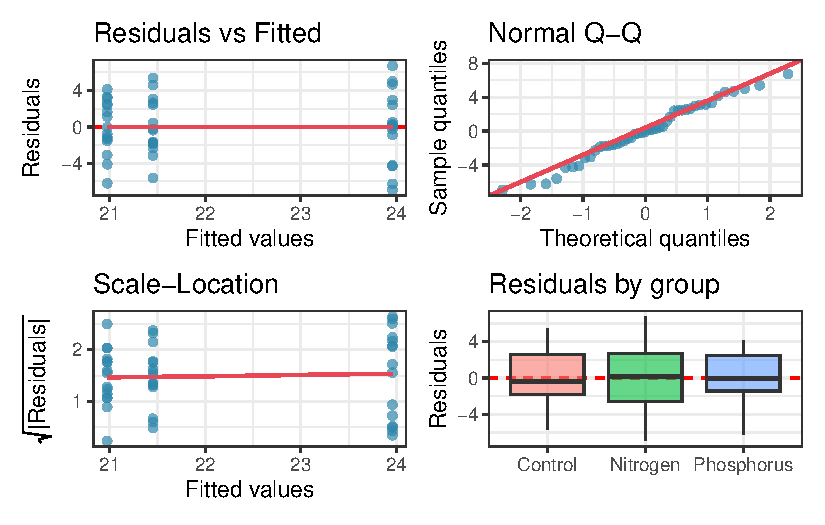
\includegraphics[width=0.9\textwidth,height=\textheight]{02b-assumptions_files/figure-pdf/unnamed-chunk-11-1.pdf}
\end{center}

\begin{verbatim}
#> 
#> --- Shapiro-Wilk test (normality of residuals) ---
#> 
#>  Shapiro-Wilk normality test
#> 
#> data:  res
#> W = 0.98099, p-value = 0.66
#> 
#> 
#> --- Levene's test (homogeneity of variance) ---
#> Levene's Test for Homogeneity of Variance (center = median)
#>       Df F value Pr(>F)
#> group  2  0.4118 0.6651
#>       42               
#> 
#> --- Diagnostic summary ---
#> Sample size (smallest group): 15 
#> Shapiro-Wilk p = 0.66 -> No evidence against normality.
#> Levene's p = 0.6651 -> No evidence against homoscedasticity.
\end{verbatim}

\subsection{The Diagnostic checklist}\label{the-diagnostic-checklist}

Before interpreting any ANOVA result, work through the following
checklist. The order matters. Start with the most consequential
assumption.

\textbf{Step 1: Independence.} Was each observation collected
independently? Are there clusters, repeated measures, or nested
structures in the data? This cannot be answered from plots alone, it
requires thinking about the study design. If independence is violated,
stop and address it before proceeding.

\textbf{Step 2: Homoscedasticity.} Look at the residuals vs fitted plot
and the residuals by group boxplot. Are the spreads roughly similar
across groups? If not, consider a transformation or switch to Welch's
ANOVA. Use Levene's test as supporting evidence, not as the primary
decision.

\textbf{Step 3: Normality.} Look at the Q-Q plot. Are the points
reasonably close to the diagonal? Is there any isolated extreme point
that might be an outlier? Use the Shapiro-Wilk test as supporting
evidence. If your sample is large and the Q-Q plot looks reasonable,
normality is almost certainly not a problem.

\textbf{Step 4: Additivity.} Is there a systematic relationship between
group means and group variances? If the groups with larger means also
show more spread, consider a log transformation before fitting the
model.

Following this workflow will not guarantee a perfect analysis, no
checklist can. But it will ensure that you have looked at your data
carefully enough to know when your conclusions are on solid ground and
when they should be treated with caution.

\part{Classical ANOVA Models}

You are unlikely to discover something new without a lot of practice on
old stuff.

--- Richard Feynman

\chapter{One-Way ANOVA}\label{sec-chap3}

The analysis of variance is not a mathematical theorem, but rather a
convenient method of arranging the arithmetic.

--- Ronald A. Fisher

One-way ANOVA is the simplest member of the ANOVA family: one response
variable, one categorical predictor, any number of groups. Despite its
simplicity, it contains all the essential ideas, variance decomposition,
the \(F\) ratio, effect sizes, power, that carry forward into every more
complex design. Mastering it thoroughly is therefore time well spent.

This chapter builds the one-way ANOVA from its mathematical foundations,
works through a complete clinical example from raw data to
interpretation, and then addresses two questions that are too often
skipped: how large is the effect, and did the experiment have enough
observations to detect it?

\section{\texorpdfstring{Model formulation and the
\(F\)-ratio}{Model formulation and the F-ratio}}\label{model-formulation-and-the-f-ratio}

\subsection{The Statistical Model}\label{the-statistical-model}

The one-way ANOVA model states that every observation \(y_{ij}\), the
\(i\)th observation in group \(j\), can be written as:

\[y_{ij} = \mu + \alpha_j + \varepsilon_{ij}\]

where:

\begin{itemize}
\tightlist
\item
  \(\mu\) is the \textbf{grand mean}: the overall mean of the response
  across all groups and all observations.
\item
  \(\alpha_j\) is the \textbf{treatment effect} of group \(j\): the
  amount by which the mean of group \(j\) departs from the grand mean.
  By convention, the treatment effects sum to zero:
  \(\sum_{j=1}^{k} \alpha_j = 0\).
\item
  \(\varepsilon_{ij}\) is the \textbf{residual} for observation \(i\) in
  group \(j\): the leftover variation that neither the grand mean nor
  the treatment effect can explain. We assume
  \(\varepsilon_{ij} \sim \mathcal{N}(0, \sigma^2)\), independently for
  all observations (Section~\ref{sec-why-residuals-not-raw-data}).
\item
  \(k\) is the number of groups and \(n_j\) is the number of
  observations in group \(j\).
\end{itemize}

The null hypothesis is that all treatment effects are zero:

\[H_0: \alpha_1 = \alpha_2 = \cdots = \alpha_k = 0\]

which is equivalent to saying that all group means are equal:

\[H_0: \mu_1 = \mu_2 = \cdots = \mu_k\]

The alternative hypothesis is that at least one \(\alpha_j \neq 0\), at
least one group mean differs from the others.

\subsection{Decomposing the Total
Variation}\label{decomposing-the-total-variation}

The key operation in ANOVA is to split the total variation in the data
into two additive components. For any observation \(y_{ij}\), its
departure from the grand mean \(\bar{y}\) can be written as:

\[\underbrace{y_{ij} - \bar{y}}_{\text{total deviation}}
= \underbrace{(\bar{y}_j - \bar{y})}_{\text{among-group deviation}}
+ \underbrace{(y_{ij} - \bar{y}_j)}_{\text{within-group deviation}}\]

Squaring and summing across all observations turns these deviations into
\textbf{sums of squares} (SS):

\[SS_{\text{total}} = SS_{\text{among}} + SS_{\text{within}}\]

where:

\[SS_{\text{total}}  = \sum_{j=1}^{k}\sum_{i=1}^{n_j}(y_{ij} - \bar{y})^2\]

\[SS_{\text{among}}  = \sum_{j=1}^{k} n_j(\bar{y}_j - \bar{y})^2\]

\[SS_{\text{within}} = \sum_{j=1}^{k}\sum_{i=1}^{n_j}(y_{ij} - \bar{y}_j)^2\]

\(SS_{\text{among}}\) measures how far the group means stray from the
grand mean: it captures the treatment effect plus any chance variation
among group means. \(SS_{\text{within}}\) measures the scatter of
observations around their own group mean: it captures residual variation
only.

\subsection{From Sums of Squares to Variances: Mean
Squares}\label{from-sums-of-squares-to-variances-mean-squares}

A sum of squares is not yet a variance, it grows automatically as the
number of observations increases, which would make comparisons across
studies meaningless. To obtain proper variance estimates, we divide each
sum of squares by its \textbf{degrees of freedom}:

\[MS_{\text{among}}  = \frac{SS_{\text{among}}}{k - 1}\]

\[MS_{\text{within}} = \frac{SS_{\text{within}}}{N - k}\]

where \(N = \sum_{j=1}^k n_j\) is the total number of observations. The
degrees of freedom deserve a moment's thought:

\begin{itemize}
\tightlist
\item
  \(SS_{\text{among}}\) is computed from \(k\) group means, but they are
  constrained to average to the grand mean, so only \(k - 1\) of them
  are free to vary.
\item
  \(SS_{\text{within}}\) is computed from \(N\) observations, with one
  mean estimated per group, leaving \(N - k\) degrees of freedom.
\end{itemize}

\(MS_{\text{within}}\) is an unbiased estimate of \(\sigma^2\)
regardless of whether \(H_0\) is true. \(MS_{\text{among}}\) estimates
\(\sigma^2\) only when \(H_0\) is true; when the treatment has a real
effect, it estimates \(\sigma^2 + \frac{\sum n_j \alpha_j^2}{k-1}\), a
quantity larger than \(\sigma^2\) by an amount proportional to the true
treatment effects.

\subsection{\texorpdfstring{The \(F\)
Ratio}{The F Ratio}}\label{the-f-ratio-1}

The \(F\) ratio is the natural consequence of everything above:

\[F = \frac{MS_{\text{among}}}{MS_{\text{within}}}\]

When \(H_0\) is true, both the numerator and denominator estimate
\(\sigma^2\), and \(F\) fluctuates around 1. When the treatment has a
real effect, the numerator grows while the denominator stays anchored to
\(\sigma^2\), and \(F\) climbs above 1. Under \(H_0\), this ratio
follows an \(F\)-distribution with \(k-1\) and \(N-k\) degrees of
freedom, written \(F_{k-1,\, N-k}\).

The results are conventionally summarised in an \textbf{ANOVA table}:

\begin{longtable}[]{@{}
  >{\raggedright\arraybackslash}p{(\columnwidth - 10\tabcolsep) * \real{0.3214}}
  >{\raggedright\arraybackslash}p{(\columnwidth - 10\tabcolsep) * \real{0.1429}}
  >{\raggedright\arraybackslash}p{(\columnwidth - 10\tabcolsep) * \real{0.1429}}
  >{\raggedright\arraybackslash}p{(\columnwidth - 10\tabcolsep) * \real{0.1786}}
  >{\raggedright\arraybackslash}p{(\columnwidth - 10\tabcolsep) * \real{0.1071}}
  >{\raggedright\arraybackslash}p{(\columnwidth - 10\tabcolsep) * \real{0.1071}}@{}}
\toprule\noalign{}
\begin{minipage}[b]{\linewidth}\raggedright
Source
\end{minipage} & \begin{minipage}[b]{\linewidth}\raggedright
SS
\end{minipage} & \begin{minipage}[b]{\linewidth}\raggedright
df
\end{minipage} & \begin{minipage}[b]{\linewidth}\raggedright
MS
\end{minipage} & \begin{minipage}[b]{\linewidth}\raggedright
F
\end{minipage} & \begin{minipage}[b]{\linewidth}\raggedright
p
\end{minipage} \\
\midrule\noalign{}
\endhead
\bottomrule\noalign{}
\endlastfoot
Among groups & \(SS_{\text{among}}\) & \(k-1\) & \(MS_{\text{among}}\) &
\(F\) & \(p\) \\
Within groups & \(SS_{\text{within}}\) & \(N-k\) &
\(MS_{\text{within}}\) & & \\
Total & \(SS_{\text{total}}\) & \(N-1\) & & & \\
\end{longtable}

\section{Example: Comparing treatment groups in a clinical
trial}\label{example-comparing-treatment-groups-in-a-clinical-trial}

\subsection{The Study}\label{the-study}

A clinical trial is investigating the effect of three treatments on
systolic blood pressure (\texttt{bp} in mmHg) in patients with mild
hypertension (Section~\ref{sec-systolic}). Patients are randomly
assigned to one of three groups (\texttt{group}): a control group
receiving a placebo (\texttt{Placebo}), a group receiving a low-dose
antihypertensive drug (\texttt{Low\ dose}), and a group receiving a
high-dose antihypertensive drug (\texttt{High\ dose}). After eight
weeks, systolic blood pressure is measured for each patient. There are
20 patients per group, giving \(N = 60\) observations in total.

The starting assumption is that the three treatments produce the same
mean blood pressure. The question is whether the data give us sufficient
reason to doubt this.

\subsection{Examining the Data}\label{examining-the-data}

First, we always look at the data before fitting any model.

\begin{Shaded}
\begin{Highlighting}[]
\FunctionTok{summary}\NormalTok{(systolic)}
\end{Highlighting}
\end{Shaded}

\begin{verbatim}
#>        bp               group   
#>  Min.   : 92.08   Placebo  :20  
#>  1st Qu.:129.61   Low dose :20  
#>  Median :136.62   High dose:20  
#>  Mean   :139.01                 
#>  3rd Qu.:148.76                 
#>  Max.   :177.44
\end{verbatim}

A combination of a boxplot and the individual observations gives a much
richer picture than summary statistics alone:

\begin{Shaded}
\begin{Highlighting}[]
\FunctionTok{library}\NormalTok{(ggplot2)}

\NormalTok{grand\_mean }\OtherTok{\textless{}{-}} \FunctionTok{mean}\NormalTok{(systolic}\SpecialCharTok{$}\NormalTok{bp)}

\FunctionTok{ggplot}\NormalTok{(systolic, }\FunctionTok{aes}\NormalTok{(}\AttributeTok{x =}\NormalTok{ group, }\AttributeTok{y =}\NormalTok{ bp, }\AttributeTok{fill =}\NormalTok{ group)) }\SpecialCharTok{+}
  \FunctionTok{geom\_boxplot}\NormalTok{(}\AttributeTok{alpha =} \FloatTok{0.4}\NormalTok{, }\AttributeTok{outlier.shape =} \ConstantTok{NA}\NormalTok{, }\AttributeTok{width =} \FloatTok{0.5}\NormalTok{) }\SpecialCharTok{+}
  \FunctionTok{geom\_jitter}\NormalTok{(}\AttributeTok{width =} \FloatTok{0.1}\NormalTok{, }\AttributeTok{size =} \DecValTok{2}\NormalTok{, }\AttributeTok{alpha =} \FloatTok{0.6}\NormalTok{, }\FunctionTok{aes}\NormalTok{(}\AttributeTok{colour =}\NormalTok{ group)) }\SpecialCharTok{+}
  \FunctionTok{geom\_hline}\NormalTok{(}\AttributeTok{yintercept =}\NormalTok{ grand\_mean, }\AttributeTok{linetype =} \StringTok{"dashed"}\NormalTok{, }\AttributeTok{colour =} \StringTok{"grey40"}\NormalTok{) }\SpecialCharTok{+}
  \FunctionTok{annotate}\NormalTok{(}\StringTok{"text"}\NormalTok{, }\AttributeTok{x =} \FloatTok{0.6}\NormalTok{, }\AttributeTok{y =}\NormalTok{ grand\_mean }\SpecialCharTok{+} \DecValTok{1}\NormalTok{, }\AttributeTok{label =} \StringTok{"Grand mean"}\NormalTok{, }\AttributeTok{size =} \FloatTok{3.2}\NormalTok{, }\AttributeTok{colour =} \StringTok{"grey40"}\NormalTok{) }\SpecialCharTok{+}
  \FunctionTok{scale\_fill\_manual}\NormalTok{(}\AttributeTok{values =} \FunctionTok{c}\NormalTok{(}\StringTok{"\#2E86AB"}\NormalTok{, }\StringTok{"\#F6AE2D"}\NormalTok{, }\StringTok{"\#E84855"}\NormalTok{)) }\SpecialCharTok{+}
  \FunctionTok{scale\_colour\_manual}\NormalTok{(}\AttributeTok{values =} \FunctionTok{c}\NormalTok{(}\StringTok{"\#2E86AB"}\NormalTok{, }\StringTok{"\#F6AE2D"}\NormalTok{, }\StringTok{"\#E84855"}\NormalTok{)) }\SpecialCharTok{+}
  \FunctionTok{labs}\NormalTok{(}\AttributeTok{x =} \ConstantTok{NULL}\NormalTok{, }\AttributeTok{y =} \StringTok{"Systolic blood pressure (mmHg)"}\NormalTok{) }\SpecialCharTok{+}
  \FunctionTok{theme\_bw}\NormalTok{() }\SpecialCharTok{+}
  \FunctionTok{theme}\NormalTok{(}\AttributeTok{legend.position =} \StringTok{"none"}\NormalTok{)}
\end{Highlighting}
\end{Shaded}

\begin{figure}[H]

\centering{

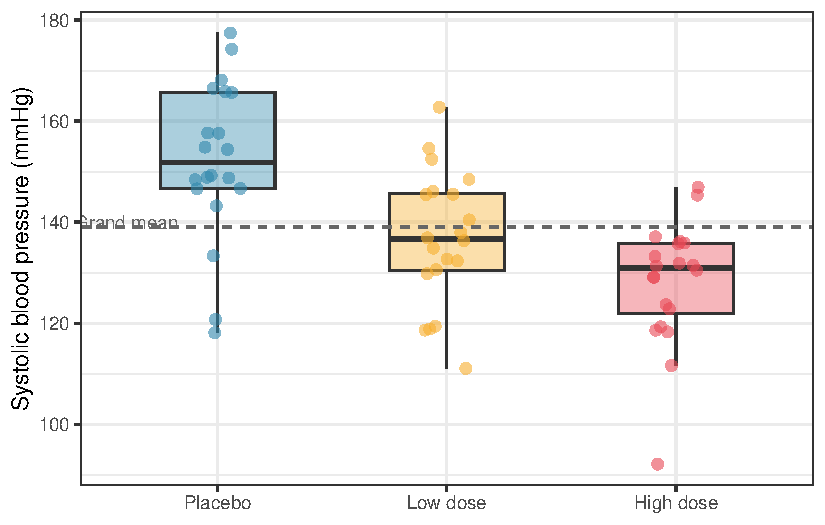
\includegraphics[width=0.9\textwidth,height=\textheight]{03a-one-way_files/figure-pdf/fig-clinical-plot-1.pdf}

}

\caption{\label{fig-clinical-plot}Systolic blood pressure (mmHg) by
treatment group. Individual observations are shown as points, jittered
horizontally to reduce overplotting. The horizontal dashed line marks
the grand mean. Even before any formal test, the progressive decrease in
both the median and spread of values from placebo to high dose is
clearly visible.}

\end{figure}%

\subsection{Checking Assumptions}\label{checking-assumptions}

Before fitting the model, we run the diagnostic workflow introduced in
Chapter \ref{sec-chap2}. Here we fit the model first in order to extract
residuals, then inspect them:

\begin{Shaded}
\begin{Highlighting}[]
\NormalTok{fit }\OtherTok{\textless{}{-}} \FunctionTok{aov}\NormalTok{(bp }\SpecialCharTok{\textasciitilde{}}\NormalTok{ group, }\AttributeTok{data =}\NormalTok{ systolic)}
\FunctionTok{anova\_diagnostics}\NormalTok{(fit, systolic)}
\end{Highlighting}
\end{Shaded}

\begin{center}
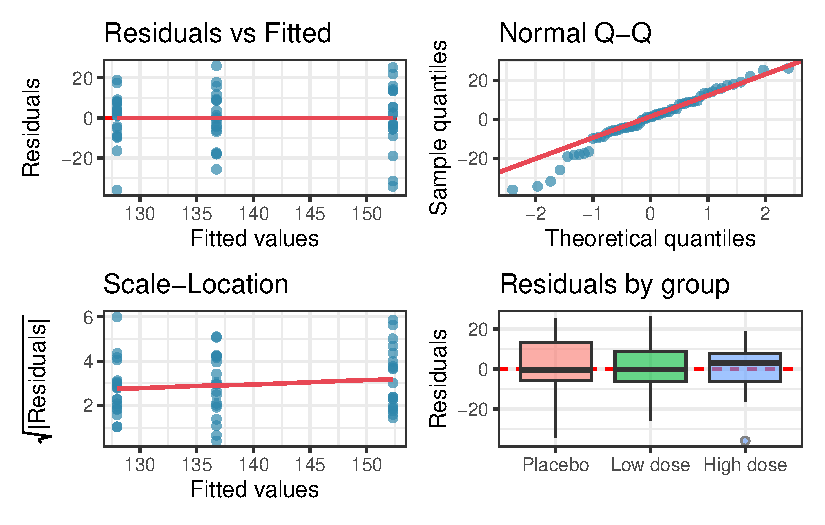
\includegraphics[width=0.9\textwidth,height=\textheight]{03a-one-way_files/figure-pdf/clinical-diagnostics-1.pdf}
\end{center}

\begin{verbatim}
#> 
#> --- Shapiro-Wilk test (normality of residuals) ---
#> 
#>  Shapiro-Wilk normality test
#> 
#> data:  res
#> W = 0.96761, p-value = 0.1114
#> 
#> 
#> --- Levene's test (homogeneity of variance) ---
#> Levene's Test for Homogeneity of Variance (center = median)
#>       Df F value Pr(>F)
#> group  2  0.7068 0.4975
#>       57               
#> 
#> --- Diagnostic summary ---
#> Sample size (smallest group): 20 
#> Shapiro-Wilk p = 0.1114 -> No evidence against normality.
#> Levene's p = 0.4975 -> No evidence against homoscedasticity.
\end{verbatim}

The Q-Q plot shows residuals lying close to the diagonal, the residual
boxplots show similar spreads across groups, and neither the
Shapiro-Wilk nor Levene's test raises any concern. We proceed with
standard one-way ANOVA.

\subsection{Fitting the Model and Reading the
Output}\label{fitting-the-model-and-reading-the-output}

The output looks like this:

\begin{Shaded}
\begin{Highlighting}[]
\FunctionTok{summary}\NormalTok{(fit)}
\end{Highlighting}
\end{Shaded}

\begin{verbatim}
#>             Df Sum Sq Mean Sq F value  Pr(>F)    
#> group        2   6066  3032.8   15.79 3.5e-06 ***
#> Residuals   57  10949   192.1                    
#> ---
#> Signif. codes:  0 '***' 0.001 '**' 0.01 '*' 0.05 '.' 0.1 ' ' 1
\end{verbatim}

Let us read this table carefully, column by column.

\begin{itemize}
\tightlist
\item
  \textbf{Df}: the degrees of freedom. The treatment factor has
  \(k - 1 = 2\) degrees of freedom (three groups minus one). The
  residuals have \(N - k = 57\) degrees of freedom (60 observations
  minus 3 groups).
\item
  \textbf{Sum Sq}: the sums of squares. The treatment accounts for 6066
  mmHg² of variation; the residuals account for 10949 mmHg².
\item
  \textbf{Mean Sq}: the mean squares, obtained by dividing each sum of
  squares by its degrees of freedom.
  \(MS_{\text{among}} = 6066 / 2 = 3032.8\);
  \(MS_{\text{within}} = 10949 / 57 = 192.1\).
\item
  \textbf{F value}: the ratio \(3032.8 / 192.1 = 15.79\). The
  among-group variance is more than 21 times larger than the
  within-group variance.
\item
  \textbf{Pr(\textgreater F)}: the probability of observing an \(F\)
  ratio this large or larger if the null hypothesis were true. Here
  \(p = 3.05 \times 10^{-6}\), an extremely small probability. We reject
  the null hypothesis and conclude that treatment group has a
  significant effect on systolic blood pressure.
\end{itemize}

\subsection{Reporting the Result}\label{reporting-the-result}

A complete report of a one-way ANOVA result should include the F
statistic, both degrees of freedom, and the p-value:

\begin{quote}
One-way ANOVA revealed a significant effect of treatment on systolic
blood pressure (\(F_{2,57} = 15.79\), \(p < 0.001\)).
\end{quote}

Note, however, that this tells us only that the groups differ, not which
specific groups differ from which. Post-hoc tests for pairwise
comparisons are covered in Chapter 5.

\section{\texorpdfstring{Effect sizes: \(\eta^2 \text{,} \omega^2\),
Cohen's
f}{Effect sizes: \textbackslash eta\^{}2 \textbackslash text\{,\} \textbackslash omega\^{}2, Cohen's f}}\label{sec-effect-size}

\subsection{Why the p-Value Is Not
Enough}\label{why-the-p-value-is-not-enough}

A significant \(p\)-value tells you that the observed differences among
groups are unlikely to be due to chance. It does not tell you how large
those differences are. This distinction matters enormously in practice.
With a large enough sample, even a trivially small treatment effect will
produce a highly significant \(p\)-value. With a small sample, a
clinically meaningful effect may fail to reach significance. The
\(p\)-value conflates the size of the effect with the size of the study.

\textbf{Effect sizes} separate these two things. They quantify how much
of the variation in the response is explained by the treatment, on a
scale that does not depend on sample size.

\subsection{A Cautionary Note: When the p-Value
Misleads}\label{a-cautionary-note-when-the-p-value-misleads}

Before moving to effect sizes formally, it is worth pausing to see
concretely why the \(p\)-value alone is insufficient for scientific
interpretation. The following simulation demonstrates the problem
directly.

We generate data from three groups whose means differ by a clinically
trivial amount, just 1 mmHg in blood pressure between groups, against a
within-group standard deviation of 12 mmHg. Nobody would consider a 1
mmHg difference between treatments to be meaningful.

We then run the same one-way ANOVA at four different sample sizes and
observe what happens to the \(p\)-value and the effect size as \(n\)
grows.

\begin{Shaded}
\begin{Highlighting}[]
\FunctionTok{library}\NormalTok{(effectsize)}

\FunctionTok{set.seed}\NormalTok{(}\DecValTok{42}\NormalTok{)}

\CommentTok{\# Trivial difference: 1 mmHg between groups, SD = 12}
\NormalTok{means }\OtherTok{\textless{}{-}} \FunctionTok{c}\NormalTok{(}\DecValTok{150}\NormalTok{, }\DecValTok{151}\NormalTok{, }\DecValTok{152}\NormalTok{)}
\NormalTok{sd\_common }\OtherTok{\textless{}{-}} \DecValTok{12}
\NormalTok{ns }\OtherTok{\textless{}{-}} \FunctionTok{c}\NormalTok{(}\DecValTok{10}\NormalTok{, }\DecValTok{50}\NormalTok{, }\DecValTok{200}\NormalTok{, }\DecValTok{2000}\NormalTok{)}

\NormalTok{results }\OtherTok{\textless{}{-}} \FunctionTok{lapply}\NormalTok{(ns, }\ControlFlowTok{function}\NormalTok{(n) \{}
\NormalTok{  group }\OtherTok{\textless{}{-}} \FunctionTok{factor}\NormalTok{(}\FunctionTok{rep}\NormalTok{(}\FunctionTok{c}\NormalTok{(}\StringTok{"Placebo"}\NormalTok{, }\StringTok{"Low dose"}\NormalTok{, }\StringTok{"High dose"}\NormalTok{), }\AttributeTok{each =}\NormalTok{ n), }\AttributeTok{levels =} \FunctionTok{c}\NormalTok{(}\StringTok{"Placebo"}\NormalTok{, }\StringTok{"Low dose"}\NormalTok{, }\StringTok{"High dose"}\NormalTok{))}
\NormalTok{  bp }\OtherTok{\textless{}{-}} \FunctionTok{c}\NormalTok{(}
    \FunctionTok{rnorm}\NormalTok{(n, }\AttributeTok{mean =}\NormalTok{ means[}\DecValTok{1}\NormalTok{], }\AttributeTok{sd =}\NormalTok{ sd\_common),}
    \FunctionTok{rnorm}\NormalTok{(n, }\AttributeTok{mean =}\NormalTok{ means[}\DecValTok{2}\NormalTok{], }\AttributeTok{sd =}\NormalTok{ sd\_common),}
    \FunctionTok{rnorm}\NormalTok{(n, }\AttributeTok{mean =}\NormalTok{ means[}\DecValTok{3}\NormalTok{], }\AttributeTok{sd =}\NormalTok{ sd\_common)}
\NormalTok{  )}
\NormalTok{  df }\OtherTok{\textless{}{-}} \FunctionTok{data.frame}\NormalTok{(bp, group)}
\NormalTok{  fit }\OtherTok{\textless{}{-}} \FunctionTok{aov}\NormalTok{(bp }\SpecialCharTok{\textasciitilde{}}\NormalTok{ group, }\AttributeTok{data =}\NormalTok{ df)}
  
\NormalTok{  p\_val }\OtherTok{\textless{}{-}} \FunctionTok{summary}\NormalTok{(fit)[[}\DecValTok{1}\NormalTok{]][[}\StringTok{"Pr(\textgreater{}F)"}\NormalTok{]][}\DecValTok{1}\NormalTok{]}
\NormalTok{  omega2 }\OtherTok{\textless{}{-}} \FunctionTok{omega\_squared}\NormalTok{(fit, }\AttributeTok{partial =} \ConstantTok{FALSE}\NormalTok{)}\SpecialCharTok{$}\NormalTok{Omega2}

  \FunctionTok{data.frame}\NormalTok{(}
    \AttributeTok{n =}\NormalTok{ n,}
    \AttributeTok{p\_val =}\NormalTok{ p\_val,}
    \AttributeTok{omega2 =}\NormalTok{ omega2}
\NormalTok{  )}
\NormalTok{\})}

\NormalTok{results\_df }\OtherTok{\textless{}{-}} \FunctionTok{do.call}\NormalTok{(rbind, results)}
\NormalTok{results\_df}\SpecialCharTok{$}\NormalTok{n\_label }\OtherTok{\textless{}{-}} \FunctionTok{paste0}\NormalTok{(}\StringTok{"n = "}\NormalTok{, results\_df}\SpecialCharTok{$}\NormalTok{n, }\StringTok{" per group"}\NormalTok{)}
\NormalTok{results\_df}\SpecialCharTok{$}\NormalTok{n\_label }\OtherTok{\textless{}{-}} \FunctionTok{factor}\NormalTok{(results\_df}\SpecialCharTok{$}\NormalTok{n\_label, }\AttributeTok{levels =} \FunctionTok{paste0}\NormalTok{(}\StringTok{"n = "}\NormalTok{, ns, }\StringTok{" per group"}\NormalTok{))}
\NormalTok{results\_df}\SpecialCharTok{$}\NormalTok{significant }\OtherTok{\textless{}{-}} \FunctionTok{ifelse}\NormalTok{(results\_df}\SpecialCharTok{$}\NormalTok{p\_val }\SpecialCharTok{\textless{}} \FloatTok{0.05}\NormalTok{, }\StringTok{"p \textless{} 0.05"}\NormalTok{, }\StringTok{"p ≥ 0.05"}\NormalTok{)}
\end{Highlighting}
\end{Shaded}

\begin{Shaded}
\begin{Highlighting}[]
\NormalTok{results\_df}
\end{Highlighting}
\end{Shaded}

\begin{verbatim}
#>      n        p_val      omega2            n_label significant
#> 1   10 4.787806e-01 0.000000000   n = 10 per group    p ≥ 0.05
#> 2   50 5.304923e-01 0.000000000   n = 50 per group    p ≥ 0.05
#> 3  200 5.005470e-01 0.000000000  n = 200 per group    p ≥ 0.05
#> 4 2000 1.466471e-06 0.004137075 n = 2000 per group    p < 0.05
\end{verbatim}

\begin{Shaded}
\begin{Highlighting}[]
\FunctionTok{library}\NormalTok{(ggplot2)}

\CommentTok{\# Plot p{-}values}
\NormalTok{p1 }\OtherTok{\textless{}{-}} \FunctionTok{ggplot}\NormalTok{(results\_df, }\FunctionTok{aes}\NormalTok{(}\AttributeTok{x =}\NormalTok{ n\_label, }\AttributeTok{y =}\NormalTok{ p\_val, }\AttributeTok{fill =}\NormalTok{ significant)) }\SpecialCharTok{+}
  \FunctionTok{geom\_col}\NormalTok{(}\AttributeTok{width =} \FloatTok{0.5}\NormalTok{) }\SpecialCharTok{+}
  \FunctionTok{geom\_hline}\NormalTok{(}\AttributeTok{yintercept =} \FloatTok{0.05}\NormalTok{, }\AttributeTok{linetype =} \StringTok{"dashed"}\NormalTok{, }\AttributeTok{colour =} \StringTok{"red"}\NormalTok{, }\AttributeTok{linewidth =} \FloatTok{0.8}\NormalTok{) }\SpecialCharTok{+}
  \FunctionTok{annotate}\NormalTok{(}\StringTok{"text"}\NormalTok{, }\AttributeTok{x =} \FloatTok{0.6}\NormalTok{, }\AttributeTok{y =} \FloatTok{0.07}\NormalTok{, }\AttributeTok{label =} \StringTok{"p = 0.05"}\NormalTok{, }\AttributeTok{colour =} \StringTok{"red"}\NormalTok{, }\AttributeTok{size =} \FloatTok{3.2}\NormalTok{, }\AttributeTok{hjust =} \DecValTok{0}\NormalTok{) }\SpecialCharTok{+}
  \FunctionTok{scale\_fill\_manual}\NormalTok{(}\AttributeTok{values =} \FunctionTok{c}\NormalTok{(}\StringTok{"p \textless{} 0.05"} \OtherTok{=} \StringTok{"\#E84855"}\NormalTok{, }\StringTok{"p ≥ 0.05"} \OtherTok{=} \StringTok{"\#2E86AB"}\NormalTok{)) }\SpecialCharTok{+}
  \FunctionTok{scale\_y\_continuous}\NormalTok{(}\AttributeTok{limits =} \FunctionTok{c}\NormalTok{(}\DecValTok{0}\NormalTok{, }\DecValTok{1}\NormalTok{)) }\SpecialCharTok{+}
  \FunctionTok{labs}\NormalTok{(}\AttributeTok{title =} \StringTok{"p{-}value"}\NormalTok{, }\AttributeTok{x =} \ConstantTok{NULL}\NormalTok{, }\AttributeTok{y =} \StringTok{"p{-}value"}\NormalTok{, }\AttributeTok{fill =} \ConstantTok{NULL}\NormalTok{) }\SpecialCharTok{+}
  \FunctionTok{theme\_bw}\NormalTok{() }\SpecialCharTok{+}
  \FunctionTok{theme}\NormalTok{(}\AttributeTok{legend.position =} \StringTok{"bottom"}\NormalTok{, }\AttributeTok{axis.text.x =} \FunctionTok{element\_text}\NormalTok{(}\AttributeTok{angle =} \DecValTok{20}\NormalTok{, }\AttributeTok{hjust =} \DecValTok{1}\NormalTok{))}

\CommentTok{\# Plot omega{-}squared}
\NormalTok{p2 }\OtherTok{\textless{}{-}} \FunctionTok{ggplot}\NormalTok{(results\_df, }\FunctionTok{aes}\NormalTok{(}\AttributeTok{x =}\NormalTok{ n\_label, }\AttributeTok{y =}\NormalTok{ omega2)) }\SpecialCharTok{+}
  \FunctionTok{geom\_col}\NormalTok{(}\AttributeTok{width =} \FloatTok{0.5}\NormalTok{, }\AttributeTok{fill =} \StringTok{"\#F6AE2D"}\NormalTok{) }\SpecialCharTok{+}
  \FunctionTok{geom\_hline}\NormalTok{(}\AttributeTok{yintercept =} \FloatTok{0.01}\NormalTok{,}
             \AttributeTok{linetype =} \StringTok{"dashed"}\NormalTok{, }\AttributeTok{colour =} \StringTok{"grey40"}\NormalTok{, }\AttributeTok{linewidth =} \FloatTok{0.8}\NormalTok{) }\SpecialCharTok{+}
  \FunctionTok{annotate}\NormalTok{(}\StringTok{"text"}\NormalTok{, }\AttributeTok{x =} \FloatTok{0.6}\NormalTok{, }\AttributeTok{y =} \FloatTok{0.013}\NormalTok{,}
           \AttributeTok{label =} \StringTok{"Small effect threshold (0.01)"}\NormalTok{,}
           \AttributeTok{colour =} \StringTok{"grey40"}\NormalTok{, }\AttributeTok{size =} \FloatTok{3.2}\NormalTok{, }\AttributeTok{hjust =} \DecValTok{0}\NormalTok{) }\SpecialCharTok{+}
  \FunctionTok{scale\_y\_continuous}\NormalTok{(}\AttributeTok{limits =} \FunctionTok{c}\NormalTok{(}\DecValTok{0}\NormalTok{, }\FloatTok{0.05}\NormalTok{)) }\SpecialCharTok{+}
  \FunctionTok{labs}\NormalTok{(}\AttributeTok{title =} \FunctionTok{expression}\NormalTok{(omega}\SpecialCharTok{\^{}}\DecValTok{2}\SpecialCharTok{\textasciitilde{}}\StringTok{"(effect size)"}\NormalTok{),}
       \AttributeTok{x =} \ConstantTok{NULL}\NormalTok{, }\AttributeTok{y =} \FunctionTok{expression}\NormalTok{(omega}\SpecialCharTok{\^{}}\DecValTok{2}\NormalTok{)) }\SpecialCharTok{+}
  \FunctionTok{theme\_bw}\NormalTok{() }\SpecialCharTok{+}
  \FunctionTok{theme}\NormalTok{(}\AttributeTok{axis.text.x =} \FunctionTok{element\_text}\NormalTok{(}\AttributeTok{angle =} \DecValTok{20}\NormalTok{, }\AttributeTok{hjust =} \DecValTok{1}\NormalTok{))}

\FunctionTok{library}\NormalTok{(patchwork)}
\NormalTok{p1 }\SpecialCharTok{+}\NormalTok{ p2}
\end{Highlighting}
\end{Shaded}

\begin{figure}[H]

\centering{

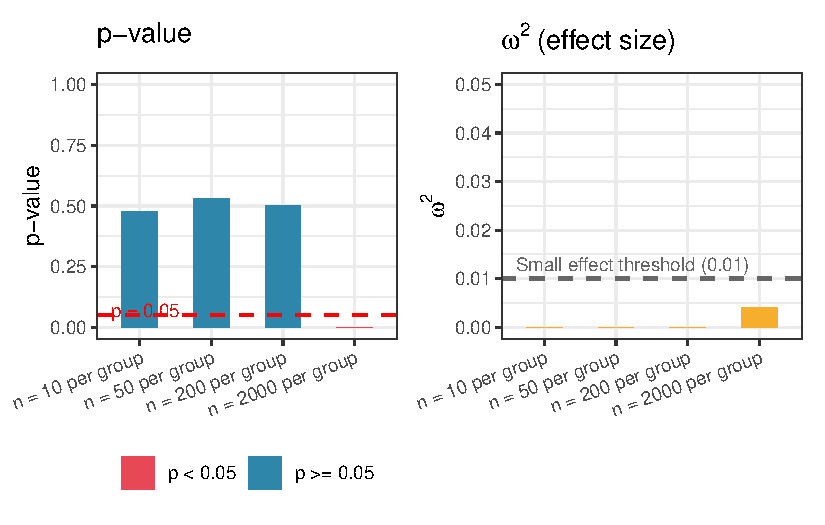
\includegraphics[width=0.9\textwidth,height=\textheight]{03a-one-way_files/figure-pdf/fig-pvalue-misleading-1.pdf}

}

\caption{\label{fig-pvalue-misleading}The same trivial effect (group
means differing by 1 mmHg against a within-group SD of 12 mmHg) analysed
at four different sample sizes. As n grows, the p-value shrinks toward
zero and eventually crosses the significance threshold not because the
effect has become more meaningful, but simply because the study has
become more sensitive. The effect size omega-squared remains negligibly
small throughout.}

\end{figure}%

The results make the problem vivid. With \(n = 10\) per group the
\(p\)-value is large and the result is non-significant but not because
the effect is small but simply because the study is underpowered. It is
only with \(n = 2000\) per group that the result is declared significant
and at that point the \(p\)-value is vanishingly small, suggesting to
anyone reading only that number that something important has been found.

Yet \(\omega^2\) tells a completely different story. Across all four
sample sizes, the effect size hovers near zero, well below even the
conventional threshold for a small effect. The treatment explains less
than 1\% of the variation in blood pressure at every sample size. The 1
mmHg difference between groups is real in a narrow statistical sense, it
is consistently detected once the sample is large enough, but it is
scientifically and clinically meaningless. What changed between
\(n = 200\) and \(n = 2000\) was not the biology. It was simply the
resolving power of the microscope.

The lesson is not that \(p\)-values are useless. They answer a specific
and legitimate question: given the data, how surprising would this
result be if there were no effect? But that question is not the same as
\emph{how large is the effect?} A \(p\)-value cannot tell you whether a
significant result matters. Only an effect size can do that.

This is why the rest of this chapter treats effect sizes not as an
optional supplement to the ANOVA table but as an essential part of every
analysis.

\subsection{\texorpdfstring{\(\eta^2\):
Eta-Squared}{\textbackslash eta\^{}2: Eta-Squared}}\label{eta2-eta-squared}

The simplest effect size for ANOVA is \(\eta^2\) (eta-squared), defined
as the proportion of total variation explained by the treatment:

\[\eta^2 = \frac{SS_{\text{among}}}{SS_{\text{total}}}\]

It ranges from 0 (treatment explains none of the variation) to 1
(treatment explains all of it). For our clinical example:

\begin{Shaded}
\begin{Highlighting}[]
\NormalTok{ss\_among }\OtherTok{\textless{}{-}} \FunctionTok{summary}\NormalTok{(fit)[[}\DecValTok{1}\NormalTok{]][}\StringTok{"group"}\NormalTok{, }\StringTok{"Sum Sq"}\NormalTok{]}
\NormalTok{ss\_total }\OtherTok{\textless{}{-}} \FunctionTok{sum}\NormalTok{(}\FunctionTok{summary}\NormalTok{(fit)[[}\DecValTok{1}\NormalTok{]][}\StringTok{"Sum Sq"}\NormalTok{])}

\NormalTok{eta2 }\OtherTok{\textless{}{-}}\NormalTok{ ss\_among }\SpecialCharTok{/}\NormalTok{ ss\_total}
\FunctionTok{cat}\NormalTok{(}\StringTok{"eta² ="}\NormalTok{, eta2, }\StringTok{"}\SpecialCharTok{\textbackslash{}n}\StringTok{"}\NormalTok{)}
\end{Highlighting}
\end{Shaded}

\begin{verbatim}
#> eta² = 0.3564937
\end{verbatim}

\(\eta^2 = 0.356\) means that 35.6\% of the total variation in blood
pressure is explained by treatment group, a large effect by any
standard.

The weakness of \(\eta^2\) is that it is a biased estimate of the true
population effect size: it tends to overestimate how much of the
variation in the \emph{population} is explained by the treatment,
because it is computed from the same data used to fit the model.

\subsection{\texorpdfstring{\(\omega^2\):
Omega-Squared}{\textbackslash omega\^{}2: Omega-Squared}}\label{omega2-omega-squared}

\(\omega^2\) (omega-squared) corrects for this bias and is generally
preferred when reporting results:

\[\omega^2 = \frac{SS_{\text{among}} - (k-1) \cdot MS_{\text{within}}}
                  {SS_{\text{total}} + MS_{\text{within}}}\]

\begin{Shaded}
\begin{Highlighting}[]
\NormalTok{k }\OtherTok{\textless{}{-}} \FunctionTok{nlevels}\NormalTok{(systolic}\SpecialCharTok{$}\NormalTok{group)}
\NormalTok{ms\_w }\OtherTok{\textless{}{-}} \FunctionTok{summary}\NormalTok{(fit)[[}\DecValTok{1}\NormalTok{]][}\StringTok{"Residuals"}\NormalTok{, }\StringTok{"Mean Sq"}\NormalTok{]}

\NormalTok{omega2 }\OtherTok{\textless{}{-}}\NormalTok{ (ss\_among }\SpecialCharTok{{-}}\NormalTok{ (k }\SpecialCharTok{{-}} \DecValTok{1}\NormalTok{) }\SpecialCharTok{*}\NormalTok{ ms\_w) }\SpecialCharTok{/}\NormalTok{ (ss\_total }\SpecialCharTok{+}\NormalTok{ ms\_w)}
\FunctionTok{cat}\NormalTok{(}\StringTok{"omega² ="}\NormalTok{, omega2, }\StringTok{"}\SpecialCharTok{\textbackslash{}n}\StringTok{"}\NormalTok{)}
\end{Highlighting}
\end{Shaded}

\begin{verbatim}
#> omega² = 0.3301868
\end{verbatim}

\(\omega^2\) is expected to be slightly smaller than \(\eta^2\), and the
difference is largest with small samples. With \(N = 60\) the correction
here is modest, but with \(N = 15\) or \(N = 20\) it can be substantial.

\textbf{Always report \(\omega^2\) rather than \(\eta^2\) when the
sample is small.}

Conventional benchmarks for both \(\eta^2\) and \(\omega^2\), originally
proposed by Cohen \citeyearpar{Cohen1988}, are:

\begin{longtable}[]{@{}lccc@{}}
\toprule\noalign{}
Effect size & Small & Medium & Large \\
\midrule\noalign{}
\endhead
\bottomrule\noalign{}
\endlastfoot
\(\eta^2\), \(\omega^2\) & 0.01 & 0.06 & 0.14 \\
\end{longtable}

These are rough guides, not rigid rules. What constitutes a meaningful
effect depends entirely on the scientific context. A drug that explains
5\% of variation in blood pressure across a population might represent
an enormous public health benefit; the same effect size in a laboratory
assay might be scientifically uninteresting.

\subsection{\texorpdfstring{Cohen's \(f\)}{Cohen's f}}\label{cohens-f}

Cohen's \(f\) is an alternative effect size that expresses the treatment
effect as the ratio of the standard deviation of group means to the
common within-group standard deviation:

\[f = \sqrt{\frac{\eta^2}{1 - \eta^2}}\]

\begin{Shaded}
\begin{Highlighting}[]
\NormalTok{f }\OtherTok{\textless{}{-}} \FunctionTok{sqrt}\NormalTok{(eta2 }\SpecialCharTok{/}\NormalTok{ (}\DecValTok{1} \SpecialCharTok{{-}}\NormalTok{ eta2))}
\FunctionTok{cat}\NormalTok{(}\StringTok{"Cohen\textquotesingle{}s f ="}\NormalTok{, }\FunctionTok{round}\NormalTok{(f, }\DecValTok{3}\NormalTok{), }\StringTok{"}\SpecialCharTok{\textbackslash{}n}\StringTok{"}\NormalTok{)}
\end{Highlighting}
\end{Shaded}

\begin{verbatim}
#> Cohen's f = 0.744
\end{verbatim}

Cohen's \(f\) is less intuitive than \(\eta^2\) or \(\omega^2\) but is
the effect size used by most power analysis software, including the
\texttt{pwr} package in R. Conventional benchmarks are \(f = 0.10\)
(small), \(f = 0.25\) (medium), and \(f = 0.40\) (large)
\citep{Cohen1988}.

\subsection{\texorpdfstring{Computing Effect Sizes with
\texttt{effectsize}}{Computing Effect Sizes with effectsize}}\label{computing-effect-sizes-with-effectsize}

Rather than computing these by hand, the \texttt{effectsize} package
provides clean, well-documented functions with confidence intervals:

\begin{Shaded}
\begin{Highlighting}[]
\CommentTok{\# install.packages("effectsize") if needed}
\FunctionTok{library}\NormalTok{(effectsize)}

\FunctionTok{eta\_squared}\NormalTok{(fit, }\AttributeTok{partial =} \ConstantTok{FALSE}\NormalTok{)}
\end{Highlighting}
\end{Shaded}

\begin{verbatim}
#> # Effect Size for ANOVA (Type I)
#> 
#> Parameter | Eta2 |       95% CI
#> -------------------------------
#> group     | 0.36 | [0.19, 1.00]
#> 
#> - One-sided CIs: upper bound fixed at [1.00].
\end{verbatim}

\begin{Shaded}
\begin{Highlighting}[]
\FunctionTok{omega\_squared}\NormalTok{(fit, }\AttributeTok{partial =} \ConstantTok{FALSE}\NormalTok{)}
\end{Highlighting}
\end{Shaded}

\begin{verbatim}
#> # Effect Size for ANOVA (Type I)
#> 
#> Parameter | Omega2 |       95% CI
#> ---------------------------------
#> group     |   0.33 | [0.16, 1.00]
#> 
#> - One-sided CIs: upper bound fixed at [1.00].
\end{verbatim}

\begin{Shaded}
\begin{Highlighting}[]
\FunctionTok{cohens\_f}\NormalTok{(fit)}
\end{Highlighting}
\end{Shaded}

\begin{verbatim}
#> For one-way between subjects designs, partial eta squared is equivalent
#>   to eta squared. Returning eta squared.
\end{verbatim}

\begin{verbatim}
#> # Effect Size for ANOVA
#> 
#> Parameter | Cohen's f |      95% CI
#> -----------------------------------
#> group     |      0.74 | [0.48, Inf]
#> 
#> - One-sided CIs: upper bound fixed at [Inf].
\end{verbatim}

Always report effect sizes alongside \(p\)-values. A result reported as
``\(F_{2,57} = 21.34\), \(p < 0.001\), \(\omega^2 = 0.36\)'' tells a
much more complete scientific story than the \(p\)-value alone.

\section{Power analysis and sample size
planning}\label{sec-power-analysis}

\subsection{What Is Statistical Power?}\label{what-is-statistical-power}

The \(F\) test can make two kinds of error.

A \textbf{Type I error} occurs when you reject \(H_0\) when it is
actually true: a false positive. The probability of a Type I error is
\(\alpha\), the significance threshold you set in advance
(conventionally 0.05).

A \textbf{Type II error} occurs when you fail to reject \(H_0\) when it
is actually false: a false negative. The probability of a Type II error
is denoted \(\beta\).

\textbf{Statistical power} is \(1 - \beta\): the probability that your
test will detect a real effect if one exists. A study with power of 0.80
has an 80\% chance of finding a significant result when the treatment
truly has an effect of the specified size.

Power depends on four quantities that are mathematically linked:

\[\text{Power} = f(\alpha,\, n,\, k,\, f)\]

\begin{itemize}
\tightlist
\item
  \textbf{\(\alpha\)}: the significance threshold. Lower \(\alpha\)
  means lower power.
\item
  \textbf{\(n\)}: the number of observations per group. More
  observations means more power.
\item
  \textbf{\(k\)}: the number of groups. More groups means more degrees
  of freedom in the numerator and generally lower power per comparison.
\item
  \textbf{\(f\)}: Cohen's \(f\), the effect size. Larger effects are
  easier to detect.
\end{itemize}

If you fix any three of these quantities, the fourth is determined. This
is the basis of power analysis.

\subsection{Prospective Power Analysis: How Many Observations Do I
Need?}\label{prospective-power-analysis-how-many-observations-do-i-need}

The most important use of power analysis is \textbf{prospective}: before
collecting data, to determine how many observations per group are needed
to detect an effect of a given size with adequate power. This requires
you to specify:

\begin{enumerate}
\def\labelenumi{\arabic{enumi}.}
\tightlist
\item
  The significance threshold \(\alpha\) (almost always 0.05).
\item
  The desired power \(1 - \beta\) (conventionally 0.80, though 0.90 is
  preferable in some situation like clinical work).
\item
  The expected effect size \(f\): the hardest quantity to specify, and
  the one that requires the most careful thought.
\end{enumerate}

In R, the \texttt{pwr} package handles this calculation:

\begin{Shaded}
\begin{Highlighting}[]
\CommentTok{\# install.packages("pwr") if needed}
\FunctionTok{library}\NormalTok{(pwr)}

\CommentTok{\# How many observations per group do we need to detect a medium effect}
\CommentTok{\# (f = 0.25) with 80\% power at alpha = 0.05, with k = 3 groups?}
\FunctionTok{pwr.anova.test}\NormalTok{(}\AttributeTok{k =} \DecValTok{3}\NormalTok{, }\AttributeTok{f =} \FloatTok{0.25}\NormalTok{, }\AttributeTok{sig.level =} \FloatTok{0.05}\NormalTok{, }\AttributeTok{power =} \FloatTok{0.80}\NormalTok{)}
\end{Highlighting}
\end{Shaded}

\begin{verbatim}
#> 
#>      Balanced one-way analysis of variance power calculation 
#> 
#>               k = 3
#>               n = 52.3966
#>               f = 0.25
#>       sig.level = 0.05
#>           power = 0.8
#> 
#> NOTE: n is number in each group
\end{verbatim}

The output show that approximately 52 observations per group, 156 in
total, are needed to detect a medium effect with 80\% power in a
three-group design. For a large effect (\(f = 0.40\)), this drops to
around 21 per group; for a small effect (\(f = 0.10\)), it rises to over
320 per group.

\subsection{Visualising the Power
Curve}\label{visualising-the-power-curve}

It is more informative to visualise how power changes across a range of
sample sizes for different effect sizes, rather than reading off a
single number:

\begin{Shaded}
\begin{Highlighting}[]
\FunctionTok{library}\NormalTok{(ggplot2)}
\FunctionTok{library}\NormalTok{(pwr)}

\NormalTok{ns }\OtherTok{\textless{}{-}} \FunctionTok{seq}\NormalTok{(}\DecValTok{5}\NormalTok{, }\DecValTok{150}\NormalTok{, }\AttributeTok{by =} \DecValTok{1}\NormalTok{)}
\NormalTok{f\_vals }\OtherTok{\textless{}{-}} \FunctionTok{c}\NormalTok{(}\FloatTok{0.10}\NormalTok{, }\FloatTok{0.25}\NormalTok{, }\FloatTok{0.40}\NormalTok{)}
\NormalTok{labels }\OtherTok{\textless{}{-}} \FunctionTok{c}\NormalTok{(}\StringTok{"Small (f = 0.10)"}\NormalTok{, }\StringTok{"Medium (f = 0.25)"}\NormalTok{, }\StringTok{"Large (f = 0.40)"}\NormalTok{)}

\NormalTok{power\_df }\OtherTok{\textless{}{-}} \FunctionTok{do.call}\NormalTok{(rbind, }\FunctionTok{lapply}\NormalTok{(}\FunctionTok{seq\_along}\NormalTok{(f\_vals), }\ControlFlowTok{function}\NormalTok{(j) \{}
  \FunctionTok{data.frame}\NormalTok{(}
    \AttributeTok{n =}\NormalTok{ ns,}
    \AttributeTok{power =} \FunctionTok{sapply}\NormalTok{(ns, }\ControlFlowTok{function}\NormalTok{(n) \{}
      \FunctionTok{pwr.anova.test}\NormalTok{(}\AttributeTok{k =} \DecValTok{3}\NormalTok{, }\AttributeTok{n =}\NormalTok{ n, }\AttributeTok{f =}\NormalTok{ f\_vals[j], }\AttributeTok{sig.level =} \FloatTok{0.05}\NormalTok{)}\SpecialCharTok{$}\NormalTok{power}
\NormalTok{    \}),}
    \AttributeTok{effect =}\NormalTok{ labels[j]}
\NormalTok{  )}
\NormalTok{\}))}

\NormalTok{power\_df}\SpecialCharTok{$}\NormalTok{effect }\OtherTok{\textless{}{-}} \FunctionTok{factor}\NormalTok{(power\_df}\SpecialCharTok{$}\NormalTok{effect, }\AttributeTok{levels =}\NormalTok{ labels)}

\FunctionTok{ggplot}\NormalTok{(power\_df, }\FunctionTok{aes}\NormalTok{(}\AttributeTok{x =}\NormalTok{ n, }\AttributeTok{y =}\NormalTok{ power, }\AttributeTok{colour =}\NormalTok{ effect)) }\SpecialCharTok{+}
  \FunctionTok{geom\_line}\NormalTok{(}\AttributeTok{linewidth =} \DecValTok{1}\NormalTok{) }\SpecialCharTok{+}
  \FunctionTok{geom\_hline}\NormalTok{(}\AttributeTok{yintercept =} \FloatTok{0.80}\NormalTok{, }\AttributeTok{linetype =} \StringTok{"dashed"}\NormalTok{, }\AttributeTok{colour =} \StringTok{"grey40"}\NormalTok{) }\SpecialCharTok{+}
  \FunctionTok{annotate}\NormalTok{(}\StringTok{"text"}\NormalTok{, }\AttributeTok{x =} \DecValTok{148}\NormalTok{, }\AttributeTok{y =} \FloatTok{0.77}\NormalTok{, }\AttributeTok{label =} \StringTok{"80\% power"}\NormalTok{, }\AttributeTok{size =} \FloatTok{3.2}\NormalTok{, }\AttributeTok{colour =} \StringTok{"grey40"}\NormalTok{, }\AttributeTok{hjust =} \DecValTok{1}\NormalTok{) }\SpecialCharTok{+}
  \FunctionTok{scale\_colour\_manual}\NormalTok{(}\AttributeTok{values =} \FunctionTok{c}\NormalTok{(}\StringTok{"\#2E86AB"}\NormalTok{, }\StringTok{"\#F6AE2D"}\NormalTok{, }\StringTok{"\#E84855"}\NormalTok{)) }\SpecialCharTok{+}
  \FunctionTok{scale\_y\_continuous}\NormalTok{(}\AttributeTok{limits =} \FunctionTok{c}\NormalTok{(}\DecValTok{0}\NormalTok{, }\DecValTok{1}\NormalTok{), }\AttributeTok{labels =}\NormalTok{ scales}\SpecialCharTok{::}\FunctionTok{percent\_format}\NormalTok{(}\AttributeTok{accuracy =} \DecValTok{1}\NormalTok{)) }\SpecialCharTok{+}
  \FunctionTok{labs}\NormalTok{(}
    \AttributeTok{x =} \StringTok{"Sample size per group (n)"}\NormalTok{,}
    \AttributeTok{y =} \StringTok{"Power"}\NormalTok{,}
    \AttributeTok{colour =} \StringTok{"Effect size"}
\NormalTok{  ) }\SpecialCharTok{+}
  \FunctionTok{theme\_bw}\NormalTok{() }\SpecialCharTok{+}
  \FunctionTok{theme}\NormalTok{(}\AttributeTok{legend.position =} \StringTok{"inside"}\NormalTok{, }\AttributeTok{legend.position.inside =} \FunctionTok{c}\NormalTok{(}\FloatTok{0.82}\NormalTok{, }\FloatTok{0.25}\NormalTok{))}
\end{Highlighting}
\end{Shaded}

\begin{figure}[H]

\centering{

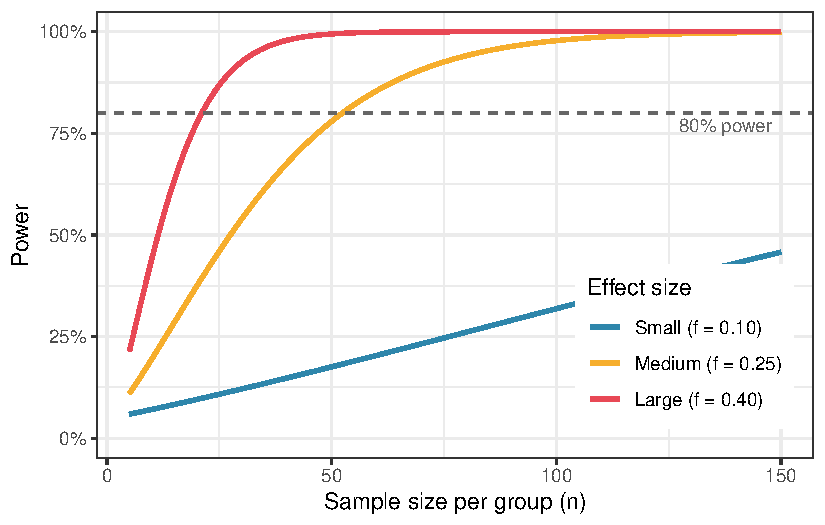
\includegraphics[width=0.9\textwidth,height=\textheight]{03a-one-way_files/figure-pdf/fig-power-curve-1.pdf}

}

\caption{\label{fig-power-curve}Power curves for a one-way ANOVA with
three groups at alpha = 0.05, across a range of sample sizes per group
and for three effect sizes. The horizontal dashed line marks the
conventional 80\% power threshold. A medium effect requires around 52
observations per group to achieve 80\% power; a small effect requires
over 300.}

\end{figure}%

\subsection{Where Does the Expected Effect Size Come
From?}\label{where-does-the-expected-effect-size-come-from}

Specifying the expected effect size is the hardest part of power
analysis, and it is where many researchers go wrong. There are three
defensible approaches.

\textbf{From prior literature.} If previous studies have measured the
same response with the same or similar treatments, use their reported
effect sizes. Be aware, however, that published effect sizes are subject
to publication bias: studies with larger effects are more likely to be
published, so the literature tends to overestimate true effect sizes.
Apply some conservatism.

\textbf{From a pilot study.} A small preliminary experiment can provide
a rough estimate of within-group variance \(\sigma\) and the expected
differences among group means, from which \(f\) can be calculated.
Pilot-based effect sizes are noisy but grounded in your specific system.

\textbf{From the minimally meaningful effect.} Ask: what is the smallest
difference among group means that would be scientifically or clinically
meaningful? For example, in the blood pressure trial, a difference of 5
mmHg between groups might be the smallest reduction considered
clinically relevant. Combined with an estimate of within-group standard
deviation (from the literature or from clinical experience), this gives
a concrete, defensible effect size to power the study for.

Using Cohen's conventional benchmarks (small, medium, large) as a
substitute for genuine subject-matter knowledge is the least
satisfactory approach, but it is better than no power analysis at all.

\subsection{Retrospective Power Analysis: A
Warning}\label{retrospective-power-analysis-a-warning}

It is tempting, after a non-significant result, to compute the power of
the completed study post hoc, to ask whether the experiment was large
enough to detect the effect that was observed. This is called
\textbf{retrospective} or \textbf{post hoc power analysis}, and it is
generally not informative. When the observed effect size is used to
compute power, a non-significant result will always produce low
estimated power, and a significant result will always produce high
estimated power. The calculation is entirely circular and adds nothing
to what the \(p\)-value already tells you.

If a study yields a non-significant result and you want to know whether
a meaningful effect might have been missed, the right tool is a
confidence interval around the effect size, not a retrospective power
calculation.

\chapter{Multiple Comparisons}\label{sec-chap4}

The \(F\) test in ANOVA answers a single, global question: do the group
means differ? When the answer is yes, the natural follow-up is:
\emph{which} groups differ from \emph{which}? This is where multiple
comparisons enter the picture and where a surprising number of otherwise
careful analyses go wrong.

The problem is not the comparisons themselves, it is doing many of them
at once without accounting for the fact that \textbf{when you ask many
questions of the same data, chance alone will eventually hand you a
significant answer}.

This chapter explains why, introduces the main corrections available in
R, and gives practical guidance on when each is appropriate.

\section{The Multiple Testing
Problem}\label{the-multiple-testing-problem}

\subsection{One Test, One Risk}\label{one-test-one-risk}

When you perform a single hypothesis test at \(\alpha = 0.05\),
\emph{you accept} a 5\% probability of a false positive which is 5\%
probability of declaring a difference significant when none truly
exists. This is the Type I error rate, and it is exactly what \(\alpha\)
controls.

\subsection{Many Tests, Compounding
Risk}\label{many-tests-compounding-risk}

Now suppose the ANOVA is significant and you want to compare all pairs
of groups. With \(k = 3\) groups, there are three pairwise comparisons:
Placebo vs Low dose, Placebo vs High dose, and Low dose vs High dose.

If you run each as a separate \(t\)-test at \(\alpha = 0.05\), the
probability of making \emph{at least one} false positive across the
three tests is no longer 5\%. Assuming the tests are independent, the
probability of making no false positives across \(m\) tests is
\((1 - \alpha)^m\), so the probability of at least one false positive
is:

\[P(\text{at least one false positive}) = 1 - (1 - \alpha)^m\]

For three tests: \(1 - (1 - 0.05)^3 = 0.143\). For five tests:
\(0.226\). For ten tests: \(0.401\). \emph{The more comparisons you
make, the more likely you are to find something significant by chance
alone}.

This inflated error rate across a family of tests is called the
\textbf{familywise error rate (FWER)}, and controlling it is the central
goal of multiple comparison procedures.

The simulation below makes this concrete. We generate data where all
groups truly have the same mean, no differences exist, and count how
often at least one pairwise \(t\)-test returns \(p < 0.05\):

\begin{Shaded}
\begin{Highlighting}[]
\FunctionTok{library}\NormalTok{(furrr)}
\FunctionTok{library}\NormalTok{(future)}
\FunctionTok{library}\NormalTok{(ggplot2)}

\FunctionTok{set.seed}\NormalTok{(}\DecValTok{42}\NormalTok{)}
\NormalTok{n\_sim }\OtherTok{\textless{}{-}} \DecValTok{5000}
\NormalTok{alpha }\OtherTok{\textless{}{-}} \FloatTok{0.05}
\NormalTok{n }\OtherTok{\textless{}{-}} \DecValTok{20}   \CommentTok{\# observations per group}

\CommentTok{\# Range of group numbers to test}
\NormalTok{k\_vals }\OtherTok{\textless{}{-}} \DecValTok{2}\SpecialCharTok{:}\DecValTok{10}

\NormalTok{fwer }\OtherTok{\textless{}{-}} \FunctionTok{future\_map\_dbl}\NormalTok{(k\_vals, }\ControlFlowTok{function}\NormalTok{(k) \{}
  
  \CommentTok{\# inner loop is sequential, parallelism at the k level only}
\NormalTok{  at\_least\_one\_fp }\OtherTok{\textless{}{-}} \FunctionTok{map\_lgl}\NormalTok{(}\FunctionTok{seq\_len}\NormalTok{(n\_sim), }\ControlFlowTok{function}\NormalTok{(i) \{}
\NormalTok{    y     }\OtherTok{\textless{}{-}} \FunctionTok{rnorm}\NormalTok{(k }\SpecialCharTok{*}\NormalTok{ n)}
\NormalTok{    group }\OtherTok{\textless{}{-}} \FunctionTok{factor}\NormalTok{(}\FunctionTok{rep}\NormalTok{(}\FunctionTok{paste0}\NormalTok{(}\StringTok{"G"}\NormalTok{, }\DecValTok{1}\SpecialCharTok{:}\NormalTok{k), }\AttributeTok{each =}\NormalTok{ n))}
\NormalTok{    df    }\OtherTok{\textless{}{-}} \FunctionTok{data.frame}\NormalTok{(y, group)}
\NormalTok{    pairs  }\OtherTok{\textless{}{-}} \FunctionTok{combn}\NormalTok{(}\FunctionTok{levels}\NormalTok{(group), }\DecValTok{2}\NormalTok{)}
\NormalTok{    p\_vals }\OtherTok{\textless{}{-}} \FunctionTok{apply}\NormalTok{(pairs, }\DecValTok{2}\NormalTok{, }\ControlFlowTok{function}\NormalTok{(g) \{}
      \FunctionTok{t.test}\NormalTok{(y }\SpecialCharTok{\textasciitilde{}}\NormalTok{ group,}
             \AttributeTok{data      =}\NormalTok{ df[df}\SpecialCharTok{$}\NormalTok{group }\SpecialCharTok{\%in\%}\NormalTok{ g, ],}
             \AttributeTok{var.equal =} \ConstantTok{TRUE}\NormalTok{)}\SpecialCharTok{$}\NormalTok{p.value}
\NormalTok{    \})}
    \FunctionTok{any}\NormalTok{(p\_vals }\SpecialCharTok{\textless{}}\NormalTok{ alpha)}
\NormalTok{  \})}
  \FunctionTok{mean}\NormalTok{(at\_least\_one\_fp)}
  
\NormalTok{\}, }\AttributeTok{.options =} \FunctionTok{furrr\_options}\NormalTok{(}\AttributeTok{seed =} \ConstantTok{TRUE}\NormalTok{))}

\FunctionTok{plan}\NormalTok{(sequential)}

\CommentTok{\# Theoretical FWER}
\NormalTok{m\_vals }\OtherTok{\textless{}{-}} \FunctionTok{choose}\NormalTok{(k\_vals, }\DecValTok{2}\NormalTok{)}
\NormalTok{fwer\_theory }\OtherTok{\textless{}{-}} \DecValTok{1} \SpecialCharTok{{-}}\NormalTok{ (}\DecValTok{1} \SpecialCharTok{{-}}\NormalTok{ alpha)}\SpecialCharTok{\^{}}\NormalTok{m\_vals}

\NormalTok{fwer\_df }\OtherTok{\textless{}{-}} \FunctionTok{data.frame}\NormalTok{(}
  \AttributeTok{k =}\NormalTok{ k\_vals,}
  \AttributeTok{m =}\NormalTok{ m\_vals,}
  \AttributeTok{fwer\_sim =}\NormalTok{ fwer,}
  \AttributeTok{fwer\_theory =}\NormalTok{ fwer\_theory}
\NormalTok{)}

\FunctionTok{ggplot}\NormalTok{(fwer\_df, }\FunctionTok{aes}\NormalTok{(}\AttributeTok{x =}\NormalTok{ k)) }\SpecialCharTok{+}
  \FunctionTok{geom\_line}\NormalTok{(}\FunctionTok{aes}\NormalTok{(}\AttributeTok{y =}\NormalTok{ fwer\_theory, }\AttributeTok{linetype =} \StringTok{"Theoretical"}\NormalTok{), }\AttributeTok{colour =} \StringTok{"\#2E86AB"}\NormalTok{, }\AttributeTok{linewidth =} \DecValTok{1}\NormalTok{) }\SpecialCharTok{+}
  \FunctionTok{geom\_point}\NormalTok{(}\FunctionTok{aes}\NormalTok{(}\AttributeTok{y =}\NormalTok{ fwer\_sim, }\AttributeTok{shape =} \StringTok{"Simulated"}\NormalTok{), }\AttributeTok{colour =} \StringTok{"\#E84855"}\NormalTok{, }\AttributeTok{size =} \DecValTok{3}\NormalTok{) }\SpecialCharTok{+}
  \FunctionTok{geom\_hline}\NormalTok{(}\AttributeTok{yintercept =}\NormalTok{ alpha, }\AttributeTok{linetype =} \StringTok{"dashed"}\NormalTok{, }\AttributeTok{colour =} \StringTok{"red"}\NormalTok{, }\AttributeTok{linewidth =} \FloatTok{0.8}\NormalTok{) }\SpecialCharTok{+}
  \FunctionTok{scale\_y\_continuous}\NormalTok{(}\AttributeTok{limits =} \FunctionTok{c}\NormalTok{(}\DecValTok{0}\NormalTok{, }\DecValTok{1}\NormalTok{), }\AttributeTok{labels =}\NormalTok{ scales}\SpecialCharTok{::}\FunctionTok{percent\_format}\NormalTok{(}\AttributeTok{accuracy =} \DecValTok{1}\NormalTok{)) }\SpecialCharTok{+}
  \FunctionTok{scale\_x\_continuous}\NormalTok{(}\AttributeTok{breaks =}\NormalTok{ k\_vals, }\AttributeTok{sec.axis =} \FunctionTok{sec\_axis}\NormalTok{(}\SpecialCharTok{\textasciitilde{}} \FunctionTok{choose}\NormalTok{(., }\DecValTok{2}\NormalTok{), }\AttributeTok{name =} \StringTok{"Number of pairwise comparisons"}\NormalTok{, }\AttributeTok{breaks =}\NormalTok{ m\_vals)) }\SpecialCharTok{+}
  \FunctionTok{scale\_linetype\_manual}\NormalTok{(}\AttributeTok{values =} \FunctionTok{c}\NormalTok{(}\StringTok{"Theoretical"} \OtherTok{=} \StringTok{"solid"}\NormalTok{)) }\SpecialCharTok{+}
  \FunctionTok{scale\_shape\_manual}\NormalTok{(}\AttributeTok{values =} \FunctionTok{c}\NormalTok{(}\StringTok{"Simulated"}   \OtherTok{=} \DecValTok{16}\NormalTok{)) }\SpecialCharTok{+}
  \FunctionTok{labs}\NormalTok{(}
    \AttributeTok{x =} \StringTok{"Number of groups (k)"}\NormalTok{,}
    \AttributeTok{y =} \StringTok{"Familywise error rate"}\NormalTok{,}
    \AttributeTok{linetype =} \ConstantTok{NULL}\NormalTok{,}
    \AttributeTok{shape =} \ConstantTok{NULL}
\NormalTok{  ) }\SpecialCharTok{+}
  \FunctionTok{theme\_bw}\NormalTok{() }\SpecialCharTok{+}
  \FunctionTok{theme}\NormalTok{(}\AttributeTok{legend.position =} \StringTok{"inside"}\NormalTok{, }\AttributeTok{legend.position.inside =} \FunctionTok{c}\NormalTok{(}\FloatTok{0.2}\NormalTok{, }\FloatTok{0.85}\NormalTok{))}
\end{Highlighting}
\end{Shaded}

\begin{figure}[H]

\centering{

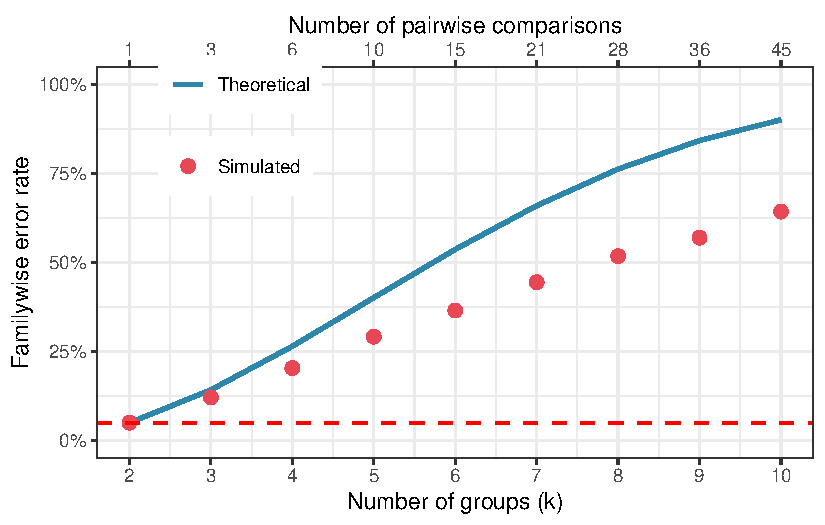
\includegraphics[width=0.9\textwidth,height=\textheight]{03b-multiple-comparisons_files/figure-pdf/fig-multiple-testing-sim-1.pdf}

}

\caption{\label{fig-multiple-testing-sim}Familywise error rate as a
function of the number of pairwise comparisons, when each test is run at
alpha = 0.05 without correction. The dashed red line marks the nominal
5\% level. With ten groups (45 pairwise comparisons), the probability of
at least one false positive exceeds 90\%.}

\end{figure}%

With just four groups and six pairwise comparisons, the familywise error
rate already exceeds 25\%. With ten groups and 45 pairwise comparisons,
it approaches 90\%.

An analyst running uncorrected pairwise \(t\)-tests after a significant
ANOVA is operating in a regime where false positives are virtually
guaranteed, not occasionally, but as a matter of arithmetic.

\subsection{Two Ways to Define the Error
Rate}\label{two-ways-to-define-the-error-rate}

Not everyone agrees that the familywise error rate is always the right
quantity to control. Two alternative perspectives are worth knowing.

The \textbf{familywise error rate (FWER)} asks: what is the probability
of making \emph{any} false positive in this family of tests? Controlling
FWER at 0.05 means that across all your comparisons, the probability of
even a single false positive is at most 5\%. This is a conservative
criterion, appropriate when any false positive would be costly, for
example, in clinical trials where a falsely declared effective treatment
might be adopted into practice.

The \textbf{false discovery rate (FDR)} asks a softer question: among
all comparisons declared significant, what proportion are expected to be
false positives? Controlling FDR at 5\% means that, on average, no more
than 5\% of your significant results are false positives. This is less
conservative than FWER control and is more appropriate in exploratory
research where missing real effects (false negatives) is considered as
costly as generating false positives.

In the context of post-hoc comparisons following a one-way ANOVA,
\emph{FWER control is the norm}. FDR control becomes more relevant in
high-dimensional settings such as genomics, where thousands of tests are
performed simultaneously.

\section{Post-Hoc Tests: Tukey, Bonferroni, Holm, and
Dunnett}\label{post-hoc-tests-tukey-bonferroni-holm-and-dunnett}

\subsection{The General Principle}\label{the-general-principle}

All post-hoc correction methods work by raising the bar for
significance, either by reducing the \(\alpha\) threshold applied to
each individual test, or by adjusting the \(p\)-values themselves
upward. They differ in how conservatively they do this, and consequently
in the balance they strike between controlling false positives and
maintaining power to detect true differences.

We will illustrate all methods using the blood pressure clinical trial
from Chapter \ref{sec-chap3}.

\subsection{Tukey's Honest Significant Difference
(HSD)}\label{tukeys-honest-significant-difference-hsd}

Tukey's HSD is the most widely used post-hoc test for pairwise
comparisons following ANOVA. It controls the familywise error rate
exactly at \(\alpha\) for all pairwise comparisons simultaneously, using
the studentised range distribution rather than the \(t\)-distribution.
It is called ``honest'' because, unlike uncorrected pairwise
\(t\)-tests, it does not overstate the evidence.

Tukey's HSD is the right default when:

\begin{itemize}
\tightlist
\item
  You want all pairwise comparisons.
\item
  Your groups have approximately equal sample sizes.
\item
  You want tight control of the familywise error rate.
\end{itemize}

\begin{Shaded}
\begin{Highlighting}[]
\NormalTok{tukey\_res }\OtherTok{\textless{}{-}} \FunctionTok{TukeyHSD}\NormalTok{(fit, }\AttributeTok{conf.level =} \FloatTok{0.95}\NormalTok{)}
\FunctionTok{print}\NormalTok{(tukey\_res)}
\end{Highlighting}
\end{Shaded}

\begin{verbatim}
#>   Tukey multiple comparisons of means
#>     95% family-wise confidence level
#> 
#> Fit: aov(formula = bp ~ group, data = systolic)
#> 
#> $group
#>                          diff       lwr        upr     p adj
#> Low dose-Placebo   -15.554942 -26.10178  -5.008100 0.0022255
#> High dose-Placebo  -24.313969 -34.86081 -13.767127 0.0000023
#> High dose-Low dose  -8.759027 -19.30587   1.787815 0.1218054
\end{verbatim}

The output gives, for each pair of groups, the estimated difference in
means, a 95\% confidence interval for that difference, and an adjusted
\(p\)-value. A confidence interval that does not include zero
corresponds to a significant difference.

It is almost always more informative to plot these intervals than to
read the table:

\begin{Shaded}
\begin{Highlighting}[]
\FunctionTok{library}\NormalTok{(ggplot2)}

\NormalTok{tukey\_df }\OtherTok{\textless{}{-}} \FunctionTok{as.data.frame}\NormalTok{(tukey\_res}\SpecialCharTok{$}\NormalTok{group)}
\NormalTok{tukey\_df}\SpecialCharTok{$}\NormalTok{comparison }\OtherTok{\textless{}{-}} \FunctionTok{rownames}\NormalTok{(tukey\_df)}
\FunctionTok{names}\NormalTok{(tukey\_df)[}\DecValTok{1}\SpecialCharTok{:}\DecValTok{4}\NormalTok{] }\OtherTok{\textless{}{-}} \FunctionTok{c}\NormalTok{(}\StringTok{"diff"}\NormalTok{, }\StringTok{"lwr"}\NormalTok{, }\StringTok{"upr"}\NormalTok{, }\StringTok{"p\_adj"}\NormalTok{)}

\FunctionTok{ggplot}\NormalTok{(tukey\_df, }\FunctionTok{aes}\NormalTok{(}\AttributeTok{x =}\NormalTok{ comparison, }\AttributeTok{y =}\NormalTok{ diff, }\AttributeTok{ymin =}\NormalTok{ lwr, }\AttributeTok{ymax =}\NormalTok{ upr)) }\SpecialCharTok{+}
  \FunctionTok{geom\_hline}\NormalTok{(}\AttributeTok{yintercept =} \DecValTok{0}\NormalTok{, }\AttributeTok{linetype =} \StringTok{"dashed"}\NormalTok{, }\AttributeTok{colour =} \StringTok{"red"}\NormalTok{, }\AttributeTok{linewidth =} \FloatTok{0.8}\NormalTok{) }\SpecialCharTok{+}
  \FunctionTok{geom\_errorbar}\NormalTok{(}\AttributeTok{width =} \FloatTok{0.15}\NormalTok{, }\AttributeTok{colour =} \StringTok{"\#2E86AB"}\NormalTok{, }\AttributeTok{linewidth =} \DecValTok{1}\NormalTok{) }\SpecialCharTok{+}
  \FunctionTok{geom\_point}\NormalTok{(}\AttributeTok{size =} \DecValTok{4}\NormalTok{, }\AttributeTok{colour =} \StringTok{"\#2E86AB"}\NormalTok{) }\SpecialCharTok{+}
  \FunctionTok{coord\_flip}\NormalTok{() }\SpecialCharTok{+}
  \FunctionTok{labs}\NormalTok{(}\AttributeTok{x =} \ConstantTok{NULL}\NormalTok{, }\AttributeTok{y =} \StringTok{"Difference in mean blood pressure (mmHg)"}\NormalTok{) }\SpecialCharTok{+}
  \FunctionTok{theme\_bw}\NormalTok{()}
\end{Highlighting}
\end{Shaded}

\begin{figure}[H]

\centering{

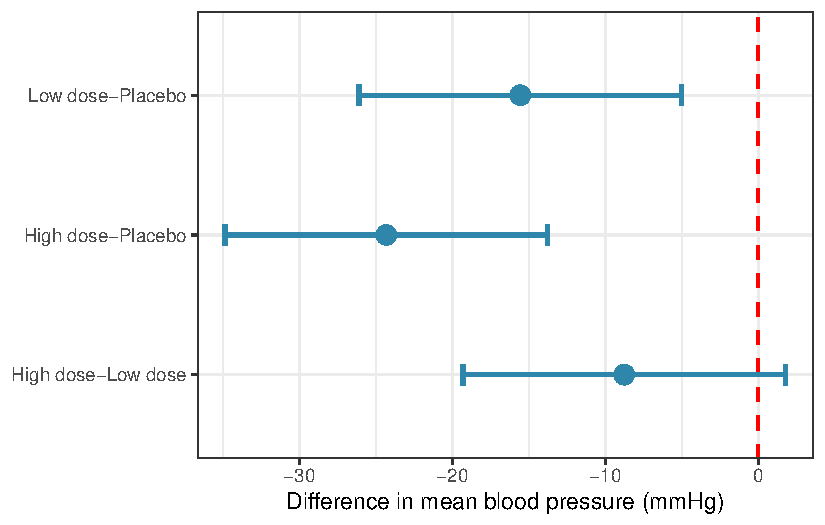
\includegraphics[width=0.9\textwidth,height=\textheight]{03b-multiple-comparisons_files/figure-pdf/fig-tukey-plot-1.pdf}

}

\caption{\label{fig-tukey-plot}Tukey HSD confidence intervals for all
pairwise comparisons of mean blood pressure. Intervals that do not cross
the vertical dashed line at zero indicate significant differences after
correction for multiple comparisons. Both active treatments differ
significantly from placebo.}

\end{figure}%

\subsection{Bonferroni Correction}\label{bonferroni-correction}

The Bonferroni correction is the simplest multiple comparison
adjustment: divide \(\alpha\) by the number of comparisons \(m\), and
declare a result significant only if its \(p\)-value falls below
\(\alpha / m\). Equivalently, multiply each \(p\)-value by \(m\) and
compare to the original \(\alpha\).

\[\alpha_{\text{Bonferroni}} = \frac{\alpha}{m}\]

For three pairwise comparisons at \(\alpha = 0.05\), each individual
test must reach \(p < 0.0167\) to be declared significant.

\begin{Shaded}
\begin{Highlighting}[]
\FunctionTok{pairwise.t.test}\NormalTok{(systolic}\SpecialCharTok{$}\NormalTok{bp, systolic}\SpecialCharTok{$}\NormalTok{group, }\AttributeTok{p.adjust.method =} \StringTok{"bonferroni"}\NormalTok{)}
\end{Highlighting}
\end{Shaded}

\begin{verbatim}
#> 
#>  Pairwise comparisons using t tests with pooled SD 
#> 
#> data:  systolic$bp and systolic$group 
#> 
#>           Placebo Low dose
#> Low dose  0.0023  -       
#> High dose 2.3e-06 0.1513  
#> 
#> P value adjustment method: bonferroni
\end{verbatim}

The Bonferroni correction is simple, transparent, and works for any
collection of tests: they do not even need to be pairwise comparisons.
Its weakness is that it is conservative: it treats all tests as
independent when in fact pairwise comparisons from the same dataset are
correlated. This means it overcorrects, throwing away real power
unnecessarily. When all pairwise comparisons are of interest, Tukey's
HSD is preferred because it accounts for the correlation structure and
is therefore less conservative.

\subsection{Holm's Method}\label{holms-method}

Holm's method is a sequential adaptation of Bonferroni that is uniformly
more powerful while still controlling the familywise error rate. It
works by ordering the \(p\)-values from smallest to largest and applying
a decreasing threshold:

\begin{enumerate}
\def\labelenumi{\arabic{enumi}.}
\tightlist
\item
  Sort the \(m\) \(p\)-values:
  \(p_{(1)} \leq p_{(2)} \leq \cdots \leq p_{(m)}\).
\item
  Compare \(p_{(1)}\) to \(\alpha / m\), \(p_{(2)}\) to
  \(\alpha / (m-1)\), and so on.
\item
  Stop at the first \(p_{(i)}\) that exceeds its threshold. Declare all
  tests from \(p_{(i)}\) onward non-significant.
\end{enumerate}

\begin{Shaded}
\begin{Highlighting}[]
\FunctionTok{pairwise.t.test}\NormalTok{(systolic}\SpecialCharTok{$}\NormalTok{bp, systolic}\SpecialCharTok{$}\NormalTok{group, }\AttributeTok{p.adjust.method =} \StringTok{"holm"}\NormalTok{)}
\end{Highlighting}
\end{Shaded}

\begin{verbatim}
#> 
#>  Pairwise comparisons using t tests with pooled SD 
#> 
#> data:  systolic$bp and systolic$group 
#> 
#>           Placebo Low dose
#> Low dose  0.0016  -       
#> High dose 2.3e-06 0.0504  
#> 
#> P value adjustment method: holm
\end{verbatim}

Holm's method should be preferred over Bonferroni in virtually every
situation. It is strictly more powerful, equally simple to explain, and
controls the FWER exactly. The only reason to use Bonferroni is when the
simplicity of a single threshold is important for communication, for
instance, when reporting to a non-statistical audience.

\subsection{Dunnett's Test}\label{dunnetts-test}

Dunnett's test is designed for a specific and common situation: you have
a control group and you want to compare each treatment group to the
control, but you are not interested in treatment-vs-treatment
comparisons. By restricting the family of comparisons to
control-vs-treatment only, Dunnett's test is more powerful than Tukey's
HSD for this specific set of comparisons.

\begin{Shaded}
\begin{Highlighting}[]
\CommentTok{\# install.packages("DescTools") if needed}
\FunctionTok{library}\NormalTok{(DescTools)}

\FunctionTok{DunnettTest}\NormalTok{(bp }\SpecialCharTok{\textasciitilde{}}\NormalTok{ group, }\AttributeTok{data =}\NormalTok{ systolic, }\AttributeTok{control =} \StringTok{"Placebo"}\NormalTok{)}
\end{Highlighting}
\end{Shaded}

\begin{verbatim}
#> 
#>   Dunnett's test for comparing several treatments with a control :  
#>     95% family-wise confidence level
#> 
#> $Placebo
#>                        diff    lwr.ci     upr.ci    pval    
#> Low dose-Placebo  -15.55494 -25.49637  -5.613511  0.0015 ** 
#> High dose-Placebo -24.31397 -34.25540 -14.372538 1.6e-06 ***
#> 
#> ---
#> Signif. codes:  0 '***' 0.001 '**' 0.01 '*' 0.05 '.' 0.1 ' ' 1
\end{verbatim}

With \(k = 3\) groups, Dunnett's test makes only 2 comparisons instead
of Tukey's 3, and the narrower family means a less severe correction,
each comparison can be more sensitive.

\subsection{Benjamini-Hochberg: Controlling the False Discovery
Rate}\label{benjamini-hochberg-controlling-the-false-discovery-rate}

Bonferroni, Holm, and Tukey all control the \textbf{familywise error
rate} i.e.~the probability of making even a single false positive. This
is a strict criterion, and its strictness has a cost: as the number of
comparisons grows, these methods become increasingly conservative,
discarding more and more true positives in order to guarantee that no
false positives slip through.

The \textbf{Benjamini-Hochberg (BH) procedure} \citep{Benjamini1995}
takes a different stance. Rather than asking ``what is the probability
of any false positive?'', it asks ``among all the comparisons I declare
significant, what fraction are expected to be false positives?'' This
fraction is called the \textbf{false discovery rate (FDR)}, and
controlling it at 5\% means that, on average, no more than 5\% of your
significant results are wrong, not that no false positives exist at all.

The procedure is straightforward:

\begin{enumerate}
\def\labelenumi{\arabic{enumi}.}
\tightlist
\item
  Sort the \(m\) \(p\)-values from smallest to largest:
  \(p_{(1)} \leq p_{(2)} \leq \cdots \leq p_{(m)}\).
\item
  Find the largest \(i\) such that
  \(p_{(i)} \leq \frac{i}{m} \cdot \alpha\).
\item
  Declare all tests up to and including rank \(i\) significant.
\end{enumerate}

In R it is simply another option in \texttt{p.adjust}:

\begin{Shaded}
\begin{Highlighting}[]
\FunctionTok{pairwise.t.test}\NormalTok{(systolic}\SpecialCharTok{$}\NormalTok{bp, systolic}\SpecialCharTok{$}\NormalTok{group, }\AttributeTok{p.adjust.method =} \StringTok{"BH"}\NormalTok{)}
\end{Highlighting}
\end{Shaded}

\begin{verbatim}
#> 
#>  Pairwise comparisons using t tests with pooled SD 
#> 
#> data:  systolic$bp and systolic$group 
#> 
#>           Placebo Low dose
#> Low dose  0.0012  -       
#> High dose 2.3e-06 0.0504  
#> 
#> P value adjustment method: BH
\end{verbatim}

The BH procedure is \textbf{uniformly more powerful than Holm and
Bonferroni}: it will declare more comparisons significant for the same
data because it tolerates a small, controlled fraction of false
positives rather than holding the false positive count to zero.

\subsection{When to Use BH vs FWER-Controlling
Methods}\label{when-to-use-bh-vs-fwer-controlling-methods}

The choice between FDR and FWER control is not a technical question, it
is a scientific one and it hinges on the consequences of each type of
error in your specific context.

\textbf{Use FWER control (Tukey, Holm) when:}

\begin{itemize}
\tightlist
\item
  Any single false positive would be costly or misleading. A falsely
  declared effective drug in a clinical trial, for example, could lead
  to harmful treatment decisions.
\item
  The number of comparisons is small (as is typical after a one-way
  ANOVA with a handful of groups).
\item
  The analysis is confirmatory: you are testing a small number of
  pre-specified hypotheses and need strong guarantees.
\end{itemize}

\textbf{Use FDR control (Benjamini-Hochberg) when:}

\begin{itemize}
\tightlist
\item
  Missing real effects is considered as costly as generating false
  positives: the balance of errors matters, not just one direction.
\item
  The number of comparisons is large, and FWER control would be so
  conservative as to be nearly useless.
\item
  The analysis is exploratory: you are screening many comparisons to
  identify candidates for further investigation, and a small fraction of
  false positives among your hits is acceptable.
\end{itemize}

The BH procedure is the dominant method in genomics and other
high-dimensional fields, where tens of thousands of tests are performed
simultaneously and FWER control would require astronomically small
individual \(p\)-value thresholds. In the context of a one-way ANOVA
with three to six groups, the practical difference between Holm and BH
will often be small with the same comparisons will reach significance.
But as the number of groups grows, or when ANOVA is used as part of a
larger screening pipeline, BH becomes the more sensible default.

The simulation below illustrates the power advantage of BH over Holm
when there are many comparisons and a mix of true and null effects:

\begin{Shaded}
\begin{Highlighting}[]
\FunctionTok{library}\NormalTok{(ggplot2)}
\FunctionTok{library}\NormalTok{(furrr)}
\FunctionTok{library}\NormalTok{(future)}

\FunctionTok{plan}\NormalTok{(multisession)}

\FunctionTok{set.seed}\NormalTok{(}\DecValTok{42}\NormalTok{)}
\NormalTok{n\_sim }\OtherTok{\textless{}{-}} \DecValTok{5000}
\NormalTok{alpha }\OtherTok{\textless{}{-}} \FloatTok{0.05}
\NormalTok{n }\OtherTok{\textless{}{-}} \DecValTok{15}
\NormalTok{k }\OtherTok{\textless{}{-}} \DecValTok{10}
\NormalTok{k\_true }\OtherTok{\textless{}{-}} \DecValTok{5}

\NormalTok{delta }\OtherTok{\textless{}{-}} \DecValTok{3}
\NormalTok{true\_means }\OtherTok{\textless{}{-}} \FunctionTok{c}\NormalTok{(}\FunctionTok{rep}\NormalTok{(delta, k\_true), }\FunctionTok{rep}\NormalTok{(}\DecValTok{0}\NormalTok{, k }\SpecialCharTok{{-}}\NormalTok{ k\_true))}

\CommentTok{\# Comparisons are G2:G10 vs G1}
\CommentTok{\# G2:G5 vs G1: both elevated by delta, truly NULL (4 comparisons)}
\CommentTok{\# G6:G10 vs G1: G1 elevated, others, not truly DIFFERENT (5 comparisons)}
\NormalTok{truly\_different }\OtherTok{\textless{}{-}} \FunctionTok{c}\NormalTok{(}\FunctionTok{rep}\NormalTok{(}\ConstantTok{FALSE}\NormalTok{, k\_true }\SpecialCharTok{{-}} \DecValTok{1}\NormalTok{),   }\CommentTok{\# G2:G5 vs G1}
                     \FunctionTok{rep}\NormalTok{(}\ConstantTok{TRUE}\NormalTok{,  k }\SpecialCharTok{{-}}\NormalTok{ k\_true))    }\CommentTok{\# G6:G10 vs G1}

\NormalTok{results }\OtherTok{\textless{}{-}} \FunctionTok{future\_map\_dfr}\NormalTok{(}\FunctionTok{seq\_len}\NormalTok{(n\_sim), }\ControlFlowTok{function}\NormalTok{(i) \{}
\NormalTok{  y }\OtherTok{\textless{}{-}} \FunctionTok{unlist}\NormalTok{(}\FunctionTok{lapply}\NormalTok{(true\_means, }\ControlFlowTok{function}\NormalTok{(m) }\FunctionTok{rnorm}\NormalTok{(n, }\AttributeTok{mean =}\NormalTok{ m, }\AttributeTok{sd =} \DecValTok{5}\NormalTok{)))}
\NormalTok{  group }\OtherTok{\textless{}{-}} \FunctionTok{factor}\NormalTok{(}\FunctionTok{rep}\NormalTok{(}\FunctionTok{paste0}\NormalTok{(}\StringTok{"G"}\NormalTok{, }\DecValTok{1}\SpecialCharTok{:}\NormalTok{k), }\AttributeTok{each =}\NormalTok{ n))}
\NormalTok{  df\_s }\OtherTok{\textless{}{-}} \FunctionTok{data.frame}\NormalTok{(y, group)}
  
\NormalTok{  p\_raw }\OtherTok{\textless{}{-}} \FunctionTok{sapply}\NormalTok{(}\FunctionTok{paste0}\NormalTok{(}\StringTok{"G"}\NormalTok{, }\DecValTok{2}\SpecialCharTok{:}\NormalTok{k), }\ControlFlowTok{function}\NormalTok{(g) \{}
    \FunctionTok{t.test}\NormalTok{(y }\SpecialCharTok{\textasciitilde{}}\NormalTok{ group,}
           \AttributeTok{data =}\NormalTok{ df\_s[df\_s}\SpecialCharTok{$}\NormalTok{group }\SpecialCharTok{\%in\%} \FunctionTok{c}\NormalTok{(}\StringTok{"G1"}\NormalTok{, g), ],}
           \AttributeTok{var.equal =} \ConstantTok{TRUE}\NormalTok{)}\SpecialCharTok{$}\NormalTok{p.value}
\NormalTok{  \})}
  
\NormalTok{  p\_holm }\OtherTok{\textless{}{-}} \FunctionTok{p.adjust}\NormalTok{(p\_raw, }\AttributeTok{method =} \StringTok{"holm"}\NormalTok{)}
\NormalTok{  p\_bh }\OtherTok{\textless{}{-}} \FunctionTok{p.adjust}\NormalTok{(p\_raw, }\AttributeTok{method =} \StringTok{"BH"}\NormalTok{)}
  
  \FunctionTok{data.frame}\NormalTok{(}
    \AttributeTok{power\_holm =} \FunctionTok{mean}\NormalTok{((p\_holm }\SpecialCharTok{\textless{}}\NormalTok{ alpha)[ truly\_different]),}
    \AttributeTok{power\_bh =} \FunctionTok{mean}\NormalTok{((p\_bh }\SpecialCharTok{\textless{}}\NormalTok{ alpha)[ truly\_different]),}
    \AttributeTok{fpr\_holm =} \FunctionTok{mean}\NormalTok{((p\_holm }\SpecialCharTok{\textless{}}\NormalTok{ alpha)[}\SpecialCharTok{!}\NormalTok{truly\_different]),}
    \AttributeTok{fpr\_bh =} \FunctionTok{mean}\NormalTok{((p\_bh }\SpecialCharTok{\textless{}}\NormalTok{ alpha)[}\SpecialCharTok{!}\NormalTok{truly\_different])}
\NormalTok{  )}
\NormalTok{\}, }\AttributeTok{.options =} \FunctionTok{furrr\_options}\NormalTok{(}\AttributeTok{seed =} \ConstantTok{TRUE}\NormalTok{))}

\NormalTok{summary\_df }\OtherTok{\textless{}{-}} \FunctionTok{data.frame}\NormalTok{(}
  \AttributeTok{metric =} \FunctionTok{c}\NormalTok{(}\StringTok{"Power}\SpecialCharTok{\textbackslash{}n}\StringTok{(true effects detected)"}\NormalTok{, }\StringTok{"False positive rate}\SpecialCharTok{\textbackslash{}n}\StringTok{(null effects declared significant)"}\NormalTok{),}
  \AttributeTok{Holm =} \FunctionTok{c}\NormalTok{(}\FunctionTok{mean}\NormalTok{(results[,}\StringTok{"power\_holm"}\NormalTok{]), }\FunctionTok{mean}\NormalTok{(results[,}\StringTok{"fpr\_holm"}\NormalTok{])),}
  \AttributeTok{BH =} \FunctionTok{c}\NormalTok{(}\FunctionTok{mean}\NormalTok{(results[,}\StringTok{"power\_bh"}\NormalTok{]), }\FunctionTok{mean}\NormalTok{(results[,}\StringTok{"fpr\_bh"}\NormalTok{]))}
\NormalTok{)}

\NormalTok{summary\_df }\OtherTok{\textless{}{-}} \FunctionTok{data.frame}\NormalTok{(}
  \AttributeTok{metric =} \FunctionTok{c}\NormalTok{(}\StringTok{"Power}\SpecialCharTok{\textbackslash{}n}\StringTok{(true effects detected)"}\NormalTok{, }\StringTok{"False positive rate}\SpecialCharTok{\textbackslash{}n}\StringTok{(null effects declared significant)"}\NormalTok{),}
  \AttributeTok{Holm =} \FunctionTok{c}\NormalTok{(}\FunctionTok{mean}\NormalTok{(results[,}\StringTok{"power\_holm"}\NormalTok{]), }\FunctionTok{mean}\NormalTok{(results[,}\StringTok{"fpr\_holm"}\NormalTok{])),}
  \AttributeTok{BH =} \FunctionTok{c}\NormalTok{(}\FunctionTok{mean}\NormalTok{(results[,}\StringTok{"power\_bh"}\NormalTok{]), }\FunctionTok{mean}\NormalTok{(results[,}\StringTok{"fpr\_bh"}\NormalTok{]))}
\NormalTok{)}

\FunctionTok{library}\NormalTok{(tidyr)}
\NormalTok{summary\_long }\OtherTok{\textless{}{-}} \FunctionTok{pivot\_longer}\NormalTok{(summary\_df, }\AttributeTok{cols =} \FunctionTok{c}\NormalTok{(}\StringTok{"Holm"}\NormalTok{, }\StringTok{"BH"}\NormalTok{), }\AttributeTok{names\_to =} \StringTok{"method"}\NormalTok{, }\AttributeTok{values\_to =} \StringTok{"value"}\NormalTok{)}

\FunctionTok{ggplot}\NormalTok{(summary\_long, }\FunctionTok{aes}\NormalTok{(}\AttributeTok{x =}\NormalTok{ method, }\AttributeTok{y =}\NormalTok{ value, }\AttributeTok{fill =}\NormalTok{ method)) }\SpecialCharTok{+}
  \FunctionTok{geom\_col}\NormalTok{(}\AttributeTok{width =} \FloatTok{0.5}\NormalTok{, }\AttributeTok{alpha =} \FloatTok{0.85}\NormalTok{) }\SpecialCharTok{+}
  \FunctionTok{geom\_hline}\NormalTok{(}\AttributeTok{yintercept =} \FloatTok{0.05}\NormalTok{, }\AttributeTok{linetype =} \StringTok{"dashed"}\NormalTok{, }\AttributeTok{colour =} \StringTok{"red"}\NormalTok{, }\AttributeTok{linewidth =} \FloatTok{0.8}\NormalTok{) }\SpecialCharTok{+}
  \FunctionTok{facet\_wrap}\NormalTok{(}\SpecialCharTok{\textasciitilde{}}\NormalTok{ metric) }\SpecialCharTok{+}
  \FunctionTok{scale\_fill\_manual}\NormalTok{(}\AttributeTok{values =} \FunctionTok{c}\NormalTok{(}\StringTok{"BH"} \OtherTok{=} \StringTok{"\#2E86AB"}\NormalTok{, }\StringTok{"Holm"} \OtherTok{=} \StringTok{"\#E84855"}\NormalTok{)) }\SpecialCharTok{+}
  \FunctionTok{scale\_y\_continuous}\NormalTok{(}\AttributeTok{limits =} \FunctionTok{c}\NormalTok{(}\DecValTok{0}\NormalTok{, }\DecValTok{1}\NormalTok{), }\AttributeTok{labels =}\NormalTok{ scales}\SpecialCharTok{::}\FunctionTok{percent\_format}\NormalTok{(}\AttributeTok{accuracy =} \DecValTok{1}\NormalTok{)) }\SpecialCharTok{+}
  \FunctionTok{labs}\NormalTok{(}\AttributeTok{x =} \ConstantTok{NULL}\NormalTok{, }\AttributeTok{y =} \ConstantTok{NULL}\NormalTok{, }\AttributeTok{fill =} \StringTok{"Method"}\NormalTok{) }\SpecialCharTok{+}
  \FunctionTok{theme\_bw}\NormalTok{() }\SpecialCharTok{+}
  \FunctionTok{theme}\NormalTok{(}\AttributeTok{legend.position =} \StringTok{"none"}\NormalTok{)}
\end{Highlighting}
\end{Shaded}

\begin{figure}[H]

\centering{

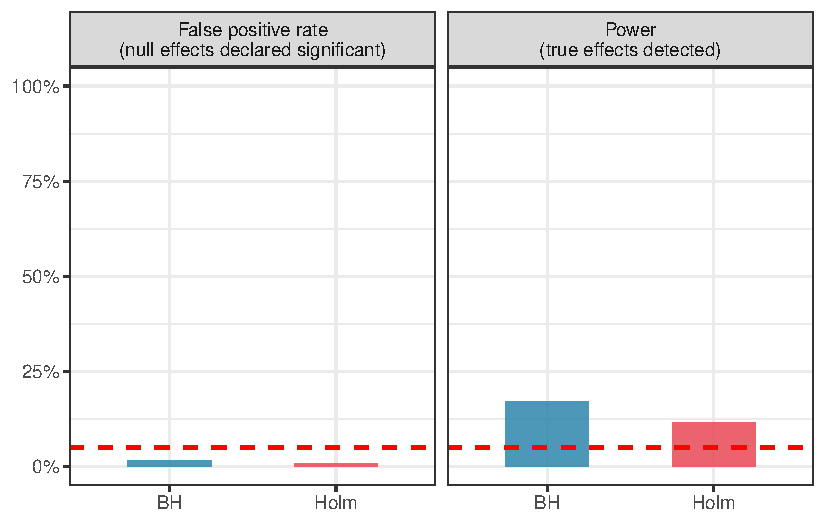
\includegraphics[width=0.9\textwidth,height=\textheight]{03b-multiple-comparisons_files/figure-pdf/fig-fdr-vs-fwer-sim-1.pdf}

}

\caption{\label{fig-fdr-vs-fwer-sim}Power and false positive rate for
Holm (FWER) and Benjamini-Hochberg (FDR) correction across 5000
simulations with k = 10 groups, half of which truly differ from the
others. BH detects more true positives (higher power) while keeping the
false discovery rate at the nominal 5\% level. Holm controls the
familywise error rate more tightly but misses more real effects.}

\end{figure}%

\subsection{Comparing the Methods}\label{comparing-the-methods}

The table below summarises the key properties of each method:

\begin{longtable}[]{@{}
  >{\raggedright\arraybackslash}p{(\columnwidth - 6\tabcolsep) * \real{0.2364}}
  >{\raggedright\arraybackslash}p{(\columnwidth - 6\tabcolsep) * \real{0.1818}}
  >{\raggedright\arraybackslash}p{(\columnwidth - 6\tabcolsep) * \real{0.2909}}
  >{\raggedright\arraybackslash}p{(\columnwidth - 6\tabcolsep) * \real{0.2909}}@{}}
\toprule\noalign{}
\begin{minipage}[b]{\linewidth}\raggedright
Method
\end{minipage} & \begin{minipage}[b]{\linewidth}\raggedright
Controls
\end{minipage} & \begin{minipage}[b]{\linewidth}\raggedright
Best used when
\end{minipage} & \begin{minipage}[b]{\linewidth}\raggedright
Relative power
\end{minipage} \\
\midrule\noalign{}
\endhead
\bottomrule\noalign{}
\endlastfoot
Tukey HSD & FWER & All pairwise, equal \(n\) & High for pairwise \\
Bonferroni & FWER & Any tests, simple communication & Low \\
Holm & FWER & Any tests, better than Bonferroni & Moderate--High \\
Dunnett & FWER & Each treatment vs one control & Highest for control
comparisons \\
Benjamini-Hochberg & FDR & Many comparisons, exploratory work &
Highest \\
\end{longtable}

\section{Planned Contrasts vs Exploratory
Comparisons}\label{planned-contrasts-vs-exploratory-comparisons}

\subsection{A Distinction That Changes the
Rules}\label{a-distinction-that-changes-the-rules}

Not all comparisons are created equal. There is a fundamental difference
between comparisons that were specified before looking at the data,
\textbf{planned contrasts}, and comparisons chosen after seeing which
groups look most different, \textbf{exploratory post-hoc comparisons}.

This distinction matters because the multiple testing problem is, at its
core, a problem of searching. \emph{When you specify your comparisons in
advance, you are not searching, you are testing a specific hypothesis}.
The number of tests you could have run but did not is irrelevant to the
interpretation of the one you did run. When you search the data for
interesting differences after the fact, every comparison you could have
made is part of the implicit search, and the familywise error rate must
reflect the size of that search.

\subsection{Planned Contrasts}\label{planned-contrasts}

A planned contrast is a specific, theoretically motivated comparison
written down before data collection. For example:

\begin{itemize}
\tightlist
\item
  ``We expect nitrogen fertiliser to increase plant height relative to
  the control, based on prior studies.''
\item
  ``We expect the average of the two drug doses to differ from
  placebo.''
\end{itemize}

Planned contrasts can be specified as linear combinations of group
means.

A contrast is a vector of coefficients \(c_j\) such that
\(\sum_{j=1}^k c_j = 0\). For example, to compare the nitrogen group
mean to the average of the control and phosphorus groups:

\[L = \bar{y}_{\text{nitrogen}} - \frac{1}{2}(\bar{y}_{\text{control}} + \bar{y}_{\text{phosphorus}})\]

with coefficients \(c = (-0.5, 1, -0.5)\) for control, nitrogen and
phosphorus respectively.

In R, planned contrasts are specified directly in the model:

\begin{Shaded}
\begin{Highlighting}[]
\CommentTok{\# Compare high dose to placebo (planned a priori)}
\CommentTok{\# and low dose to placebo (planned a priori)}
\CommentTok{\# using the multcomp package}

\CommentTok{\# install.packages("multcomp") if needed}
\FunctionTok{library}\NormalTok{(multcomp)}

\CommentTok{\# Define contrast matrix: each row is one contrast}
\CommentTok{\# Groups are ordered as: High dose, Low dose, Placebo}
\NormalTok{K }\OtherTok{\textless{}{-}} \FunctionTok{rbind}\NormalTok{(}
  \StringTok{"High dose vs Placebo"} \OtherTok{=} \FunctionTok{c}\NormalTok{(}\SpecialCharTok{{-}}\DecValTok{1}\NormalTok{,  }\DecValTok{0}\NormalTok{,  }\DecValTok{1}\NormalTok{),}
  \StringTok{"Low dose vs Placebo"}  \OtherTok{=} \FunctionTok{c}\NormalTok{( }\DecValTok{0}\NormalTok{, }\SpecialCharTok{{-}}\DecValTok{1}\NormalTok{,  }\DecValTok{1}\NormalTok{)}
\NormalTok{)}

\NormalTok{planned }\OtherTok{\textless{}{-}} \FunctionTok{glht}\NormalTok{(fit, }\AttributeTok{linfct =} \FunctionTok{mcp}\NormalTok{(}\AttributeTok{group =}\NormalTok{ K))}
\FunctionTok{summary}\NormalTok{(planned, }\AttributeTok{test =} \FunctionTok{adjusted}\NormalTok{(}\StringTok{"none"}\NormalTok{))  }\CommentTok{\# no correction for planned contrasts}
\end{Highlighting}
\end{Shaded}

\begin{verbatim}
#> 
#>   Simultaneous Tests for General Linear Hypotheses
#> 
#> Multiple Comparisons of Means: User-defined Contrasts
#> 
#> 
#> Fit: aov(formula = bp ~ group, data = systolic)
#> 
#> Linear Hypotheses:
#>                           Estimate Std. Error t value Pr(>|t|)    
#> High dose vs Placebo == 0  -24.314      4.383  -5.548 7.82e-07 ***
#> Low dose vs Placebo == 0    -8.759      4.383  -1.999   0.0504 .  
#> ---
#> Signif. codes:  0 '***' 0.001 '**' 0.01 '*' 0.05 '.' 0.1 ' ' 1
#> (Adjusted p values reported -- none method)
\end{verbatim}

\begin{Shaded}
\begin{Highlighting}[]
\FunctionTok{confint}\NormalTok{(planned)}
\end{Highlighting}
\end{Shaded}

\begin{verbatim}
#> 
#>   Simultaneous Confidence Intervals
#> 
#> Multiple Comparisons of Means: User-defined Contrasts
#> 
#> 
#> Fit: aov(formula = bp ~ group, data = systolic)
#> 
#> Quantile = 2.2682
#> 95% family-wise confidence level
#>  
#> 
#> Linear Hypotheses:
#>                           Estimate lwr      upr     
#> High dose vs Placebo == 0 -24.3140 -34.2551 -14.3728
#> Low dose vs Placebo == 0   -8.7590 -18.7002   1.1821
\end{verbatim}

Notice \texttt{adjusted("none")} because these contrasts were planned in
advance and are limited in number, no correction for multiple
comparisons is applied. The tests stand on their own as independent,
pre-specified hypotheses.

This is the important practical payoff of planning your comparisons in
advance: you preserve the full \(\alpha = 0.05\) for each test, rather
than spending part of it on the correction overhead.

\subsection{Exploratory Post-Hoc
Comparisons}\label{exploratory-post-hoc-comparisons}

When you look at the data first and then decide which groups to compare,
you are in exploratory territory. This is not wrong: exploration is a
legitimate and important part of science but it requires honest
accounting. The comparisons must be treated as a family, and the
familywise error rate must be controlled. Tukey's HSD or Holm's method
is appropriate here.

The clearest sign that you are in exploratory territory is when your
choice of comparisons is guided by the data: ``the nitrogen group looks
highest, so let me compare it to everything else.'' Any comparison
motivated by looking at the results first is post-hoc, regardless of
whether it feels like something you would have planned.

\section{Practical Guidance: When to Correct and When Not
To}\label{practical-guidance-when-to-correct-and-when-not-to}

The multiple comparisons literature contains genuine disagreement among
statisticians, and students are sometimes given conflicting advice. The
following principles represent a pragmatic, widely accepted position.

\subsection{Correct When You Are
Searching}\label{correct-when-you-are-searching}

If the comparisons were not specified in advance, correction is
necessary. The more comparisons you make, the more aggressively you
should correct. Tukey's HSD is the right default for all pairwise
comparisons following a one-way ANOVA. Holm's method is appropriate when
the set of comparisons is more varied.

\subsection{Do Not Correct Pre-Specified Planned
Contrasts}\label{do-not-correct-pre-specified-planned-contrasts}

If you specified a small number of theoretically motivated comparisons
before data collection, correction is not required and is arguably
incorrect, because you would be penalising yourself for tests you might
have run but did not. Keep the number of planned contrasts modest (as a
rough guide, no more than \(k - 1\) contrasts for \(k\) groups) and
specify them in your analysis plan before opening the data.

\subsection{Consider the Consequences of Each Error
Type}\label{consider-the-consequences-of-each-error-type}

Multiple comparison corrections reduce false positives at the cost of
increasing false negatives; they make it harder to detect real effects.
In some contexts, missing a real effect is more costly than generating a
false positive; in others, the reverse is true. A screening experiment
designed to identify candidate treatments for further investigation
might accept more false positives in exchange for fewer missed effects.
For example, a confirmatory clinical trial must be conservative about
false positives because a falsely declared effective treatment may
ultimately be adopted into clinical practice. Let the scientific
context, not habit, guide your choice of correction.

\subsection{Always Report What You
Did}\label{always-report-what-you-did}

Whatever correction you apply, or do not apply, should be stated
explicitly. Report the uncorrected \(p\)-values alongside the corrected
ones when space allows. A reader who knows you used Tukey's HSD can
evaluate your decision; a reader who does not know what correction was
applied cannot.

\subsection{A Decision Guide}\label{a-decision-guide}

\begin{figure}

\centering{


\includegraphics[width=8.79in,height=7.53in]{03b-multiple-comparisons_files/figure-latex/mermaid-figure-1.png}

}

\caption{\label{fig-comparison-decision-tree}A decision guide for
selecting a multiple comparison approach after a significant one-way
ANOVA.}

\end{figure}%

\subsection{The Bottom Line}\label{the-bottom-line}

Multiple comparison corrections are not bureaucratic box-ticking. They
exist because data can be made to say almost anything if you ask enough
questions of them. The discipline of specifying comparisons in advance,
or of honestly accounting for the number of comparisons made post-hoc,
is what separates a trustworthy analysis from one that has been, perhaps
unknowingly, optimised to produce significant results.

At the same time, correction is not always necessary, and overcorrecting
is a real error with real costs and can cause you to dismiss effects
that are genuine. The goal is calibration: matching the stringency of
your error control to the scientific context, the number of comparisons,
and the consequences of being wrong in either direction.

\chapter{Two-Way ANOVA and Factorial Designs}\label{sec-chap5}

One-way ANOVA asks whether a single factor, a fertiliser, a drug, or a
diet, affects the response. But most biological systems are not that
simple. Plant growth depends on both the fertiliser applied and the soil
type it is applied to. Drug efficacy depends on both the dose and the
genetic background of the patient. Yield depends on both the crop
variety and the environment in which it is grown.

Two-way ANOVA extends the one-way framework to handle two factors
simultaneously. This is not merely a convenience, it is a more honest
representation of how biological systems work. And it introduces one of
the most important concepts in all of applied statistics: the
\textbf{interaction}, the situation where the effect of one factor
depends on the level of another.

\section{Factorial Designs: The Logic and the
Advantage}\label{factorial-designs-the-logic-and-the-advantage}

\subsection{The One-Factor-at-a-Time
Trap}\label{the-one-factor-at-a-time-trap}

Before introducing the statistics, it is worth asking a more fundamental
question: why run a factorial experiment at all? The intuitive
alternative, varying one factor at a time while holding everything else
constant, seems safer and easier to interpret. In practice, it is
neither.

Suppose you want to understand how both fertiliser type and watering
regime affect wheat yield. The one-factor-at-a-time approach would run
two separate experiments: first vary the fertiliser while keeping
watering constant, then vary watering while keeping fertiliser constant.
This requires two experiments, two sets of plants, and twice the
resources. More importantly, it answers two questions in isolation: what
does fertiliser do when watering is fixed at one level? rather than the
richer question of how fertiliser and watering work \emph{together}
across the full range of conditions you care about.

Worst of all, the one-factor-at-a-time approach cannot detect
interactions. If nitrogen fertiliser triples yield under well-watered
conditions but has no effect under drought, two separate experiments,
one fixing watering at ``well-watered'' and one fixing fertiliser at
``nitrogen'', will never reveal this. You would need to have been lucky
enough to choose the right fixed level in each experiment, and even then
you would have no statistical framework for testing whether the
discrepancy is real or due to chance.

Fisher recognised this limitation at Rothamsted in the 1920s and
proposed the factorial design as the solution: vary all factors
simultaneously, in all combinations, within a single experiment.

\subsection{What Is a Factorial
Design?}\label{what-is-a-factorial-design}

A \textbf{factorial design} is an experiment in which every level of
every factor is combined with every level of every other factor. If
factor \(A\) has \(a\) levels and factor \(B\) has \(b\) levels, a
complete factorial design has \(a \times b\) treatment combinations,
called \textbf{cells}. With replication, \(n\) observations per cell,
the total number of observations is \(a \times b \times n\).

For our fertiliser and watering experiment with two fertiliser levels
(none, nitrogen) and two watering levels (dry, watered), a
\(2 \times 2\) factorial design produces four cells:

\begin{longtable}[]{@{}lcc@{}}
\toprule\noalign{}
& Dry & Watered \\
\midrule\noalign{}
\endhead
\bottomrule\noalign{}
\endlastfoot
\textbf{No fertiliser} & Cell 1 & Cell 2 \\
\textbf{Nitrogen} & Cell 3 & Cell 4 \\
\end{longtable}

Each cell receives its own random set of experimental units, here, pots
of wheat plants. With \(n = 5\) plants per cell, the total experiment
requires \(2 \times 2 \times 5 = 20\) plants.

\subsection{The Efficiency Advantage}\label{the-efficiency-advantage}

A factorial design extracts more information from the same data than a
one-factor-at-a-time experiment of the same size. Consider a
\(2 \times 2\) factorial with \(n\) observations per cell, giving \(4n\)
observations in total. The main effect of fertiliser is estimated by
comparing the \(2n\) observations in the nitrogen rows to the \(2n\)
observations in the no-fertiliser rows with all \(4n\) observations
contribute to this estimate. The main effect of watering is estimated
similarly, using all \(4n\) observations. A one-factor-at-a-time
experiment of the same total size would dedicate only \(2n\)
observations to each factor.

Fisher called this the \textbf{hidden replication} of factorial designs:
every observation simultaneously contributes to the estimation of every
main effect and every interaction. No observation is wasted.

\subsection{Common Factorial Design
Structures}\label{common-factorial-design-structures}

Factorial designs come in several standard forms, differing in the
number of factors and levels involved.

\begin{itemize}
\item
  \textbf{\(2 \times 2\) factorial (two factors, two levels each).} The
  simplest factorial design. Produces four cells and allows estimation
  of two main effects and one interaction. Common in clinical trials
  (drug A yes/no \(\times\) drug B yes/no) and agricultural experiments
  (fertiliser yes/no \(\times\) irrigation yes/no).
\item
  \textbf{\(2^k\) factorial (k factors, two levels each).} A natural
  extension of the \(2 \times 2\) design to \(k\) factors. With
  \(k = 3\) factors there are \(2^3 = 8\) cells; with \(k = 4\) there
  are \(2^4 = 16\) cells. These designs are widely used in industrial
  and agricultural screening experiments where many factors must be
  evaluated efficiently.
\item
  \textbf{\(a \times b\) factorial (two factors, multiple levels).} The
  general case, as in our fertiliser-by-environment example (see below)
  with four varieties and three environments (\(4 \times 3 = 12\)
  cells). This is the most common structure in biological research.
\item
  \textbf{Higher-order factorials.} Three or more factors can be
  combined in a single experiment (\(a \times b \times c\), and so on).
  These designs become large quickly: a \(3 \times 3 \times 3\)
  factorial already requires 27 cells and their higher-order
  interactions are often difficult to interpret biologically. In
  practice, three-way and higher interactions are rarely interpretable
  and the experiments that produce them often require \textbf{fractional
  factorial designs}, which are beyond the scope of this book.
\end{itemize}

\subsection{Balanced vs Unbalanced Factorial
Designs}\label{balanced-vs-unbalanced-factorial-designs}

A factorial design is \textbf{balanced} when every cell contains exactly
the same number of observations. Balanced designs have important
advantages: the main effects and interaction are orthogonal
(statistically independent), the sums of squares partition cleanly and
unambiguously, and the analysis is straightforward. Whenever possible,
factorial experiments should be designed to be balanced.

In practice, balance is often lost. Animals die, plants fail to
germinate, patients drop out of trials, soil cores are contaminated. The
result is an \textbf{unbalanced design} (unequal cell sizes) which
introduces the sums of squares complications discussed in
Section~\ref{sec-unbalanced}. The key practical message is that
unbalanced designs are manageable, but they require more care in
analysis and should be anticipated at the design stage by slightly
over-recruiting to each cell.

\subsection{Fixed, Random, and Mixed Factorial
Designs}\label{fixed-random-and-mixed-factorial-designs}

Just as in one-way ANOVA (\textbf{?@sec-one-way}), the factors in a
factorial design can be fixed or random, and this distinction determines
both the model and the correct F test.

A \textbf{fixed factor} is one whose levels are specifically chosen by
the experimenter and whose conclusions apply only to those levels.
Fertiliser type (none, nitrogen, phosphorus) is a fixed factor: the
conclusions are about those three specific treatments.

A \textbf{random factor} is one whose levels are a random sample from a
larger population of levels, and whose conclusions are intended to
generalise to that population. Field sites selected at random from a
region, batches of reagents drawn from a production run, or patients
recruited from a hospital are random factors.

A \textbf{mixed factorial design} contains both fixed and random
factors. This is extremely common in biology: a treatment applied across
randomly selected sites, a drug tested across randomly recruited
patients, or a crop variety evaluated across randomly selected growing
seasons. The statistical model for a mixed factorial design is a
\textbf{mixed-effects model}, and the correct F tests for the fixed
effects differ from those in an all-fixed design. This will be developed
fully in Part III. For now, the two-way ANOVA presented in this chapter
assumes both factors are fixed.

\subsection{Randomisation in Factorial
Designs}\label{randomisation-in-factorial-designs}

As Fisher emphasised at Rothamsted, the validity of a factorial
experiment depends on proper randomisation. Each experimental unit must
be randomly assigned to one of the \(a \times b\) treatment
combinations. This randomisation ensures that the treatment effects are
not confounded with any systematic difference between units such as
position in a greenhouse, order of processing in a laboratory, or any
other nuisance variable that might vary across the experiment.

In practice, randomisation in factorial experiments is sometimes
constrained. If one factor is difficult or expensive to change (the
temperature of a growth chamber, the irrigation regime of a field) it
may be more practical to change it less frequently than the other
factor. This leads to \textbf{split-plot designs}, in which the
randomisation is done in two stages and the two factors have different
levels of replication. Split-plot designs require a modified analysis
and are covered in Chapter 7.

The diagram below summarises the common factorial design structures
discussed in this section:

\begin{figure}

\centering{

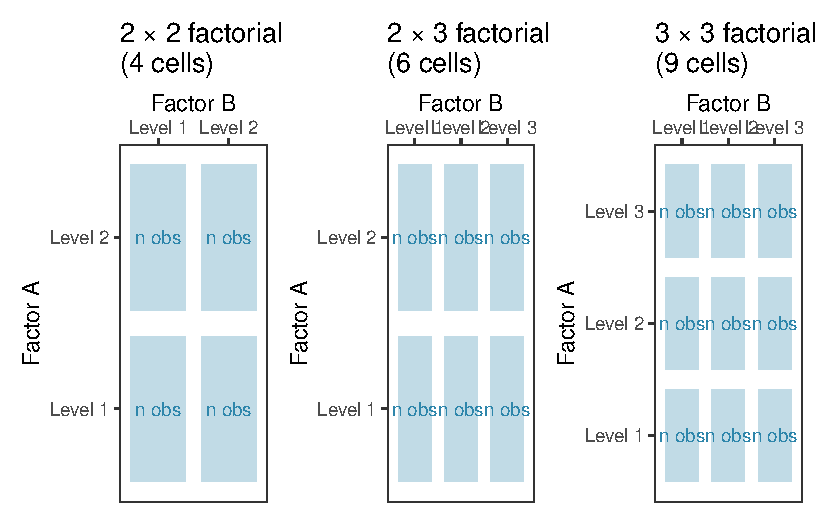
\includegraphics[width=0.9\textwidth,height=\textheight]{03c-two-way_files/figure-pdf/fig-factorial-design-diagram-1.pdf}

}

\caption{\label{fig-factorial-design-diagram}Common factorial design
structures. Left: a 2x2 factorial with two factors at two levels each,
producing four cells. Centre: a 2x3 factorial with two factors at two
and three levels respectively, producing six cells. Right: a 2x2x2
factorial with three factors at two levels each, producing eight cells.
Cell shading indicates a different treatment combination; n denotes the
number of replicate observations per cell.}

\end{figure}%

\section{Main Effects and
Interactions}\label{main-effects-and-interactions}

\subsection{The Model}\label{the-model}

With two factors \(A\) (with \(a\) levels) and \(B\) (with \(b\)
levels), the two-way ANOVA model is:

\[y_{ijk} = \mu + \alpha_i + \beta_j + (\alpha\beta)_{ij} + \varepsilon_{ijk}\]

where:

\begin{itemize}
\tightlist
\item
  \(\mu\) is the grand mean.
\item
  \(\alpha_i\) is the \textbf{main effect} of factor \(A\) at level
  \(i\): the average effect of being in level \(i\) of \(A\), averaged
  across all levels of \(B\).
\item
  \(\beta_j\) is the \textbf{main effect} of factor \(B\) at level
  \(j\): the average effect of being in level \(j\) of \(B\), averaged
  across all levels of \(A\).
\item
  \((\alpha\beta)_{ij}\) is the \textbf{interaction effect}: the extent
  to which the effect of factor \(A\) at level \(i\) differs depending
  on which level of \(B\) is present, and vice versa.
\item
  \(\varepsilon_{ijk}\) is the residual for the \(k\)th observation in
  cell \((i, j)\), assumed
  \(\varepsilon_{ijk} \sim \mathcal{N}(0, \sigma^2)\).
\end{itemize}

The constraints are \(\sum_i \alpha_i = 0\), \(\sum_j \beta_j = 0\),
\(\sum_i (\alpha\beta)_{ij} = 0\) for all \(j\), and
\(\sum_j (\alpha\beta)_{ij} = 0\) for all \(i\).

\subsection{Main Effects}\label{main-effects}

A \textbf{main effect} is the average effect of one factor, collapsing
across all levels of the other. In a fertiliser-by-watering experiment,
the main effect of fertiliser is the average difference in plant height
between fertilised and unfertilised plants, averaging over both watered
and unwatered conditions.

Main effects are straightforward to interpret, but only when the
interaction is absent or negligible. When a substantial interaction is
present, main effects can be misleading, as we will see shortly.

\subsection{Interactions}\label{interactions}

An \textbf{interaction} occurs when the effect of one factor is not the
same at every level of the other factor. This is not a statistical
artefact or a complication to be wished away, it is a genuine biological
phenomenon, and recognising it is often the most scientifically
interesting finding in an experiment.

Three situations are worth distinguishing:

\textbf{No interaction (additivity).} The effect of factor \(A\) is the
same regardless of which level of \(B\) is present. The two factors act
independently and their effects simply add together. The lines in an
interaction plot are parallel.

\textbf{Quantitative interaction.} The effect of factor \(A\) differs in
\emph{magnitude} across levels of \(B\), but always in the same
\emph{direction}. For example, nitrogen fertiliser always increases
plant height, but by more in well-watered plots than in dry plots. The
lines in an interaction plot are not parallel but do not cross.

\textbf{Qualitative interaction (crossover interaction).} The effect of
factor \(A\) reverses \emph{direction} depending on the level of \(B\).
For example, a drug increases survival in young patients but decreases
it in elderly patients. The lines in an interaction plot cross. This is
the most consequential type of interaction: main effects are not just
misleading here, they are actively wrong.

\subsection{\texorpdfstring{The Three \(F\)
Tests}{The Three F Tests}}\label{the-three-f-tests}

Two-way ANOVA produces three \(F\) tests, one for each term in the
model:

\[F_A = \frac{MS_A}{MS_{\text{within}}} \qquad
  F_B = \frac{MS_B}{MS_{\text{within}}} \qquad
  F_{AB} = \frac{MS_{AB}}{MS_{\text{within}}}\]

The interaction test \(F_{AB}\) should always be examined first. If it
is significant, the main effect tests must be interpreted with great
caution: they describe averages that may not represent any real
condition in the experiment.

\section{Interpreting Interaction Plots: A Critical
Skill}\label{interpreting-interaction-plots-a-critical-skill}

\subsection{Why Interaction Plots
Matter}\label{why-interaction-plots-matter}

An interaction plot displays the mean response for each combination of
factor levels, with the levels of one factor on the x-axis and separate
lines for each level of the other factor. It is the single most
important diagnostic tool in factorial ANOVA, and the ability to read
one correctly is a skill worth developing carefully.

The rule of thumb is simple: \textbf{parallel lines mean no interaction;
non-parallel lines suggest an interaction.} But as the simulations below
show, the details matter considerably.

\begin{Shaded}
\begin{Highlighting}[]
\FunctionTok{library}\NormalTok{(ggplot2)}
\FunctionTok{library}\NormalTok{(patchwork)}

\FunctionTok{set.seed}\NormalTok{(}\DecValTok{42}\NormalTok{)}

\NormalTok{n }\OtherTok{\textless{}{-}} \DecValTok{20}  \CommentTok{\# per cell}

\CommentTok{\# Factor levels}
\NormalTok{fertiliser }\OtherTok{\textless{}{-}} \FunctionTok{c}\NormalTok{(}\StringTok{"None"}\NormalTok{, }\StringTok{"Nitrogen"}\NormalTok{)}
\NormalTok{water }\OtherTok{\textless{}{-}} \FunctionTok{c}\NormalTok{(}\StringTok{"Dry"}\NormalTok{, }\StringTok{"Watered"}\NormalTok{)}

\NormalTok{make\_df }\OtherTok{\textless{}{-}} \ControlFlowTok{function}\NormalTok{(cell\_means, }\AttributeTok{sd =} \DecValTok{4}\NormalTok{) \{}
  \FunctionTok{data.frame}\NormalTok{(}
    \AttributeTok{height =} \FunctionTok{c}\NormalTok{(}
      \FunctionTok{rnorm}\NormalTok{(n, cell\_means[}\DecValTok{1}\NormalTok{], sd),   }\CommentTok{\# None    x Dry}
      \FunctionTok{rnorm}\NormalTok{(n, cell\_means[}\DecValTok{2}\NormalTok{], sd),   }\CommentTok{\# None    x Watered}
      \FunctionTok{rnorm}\NormalTok{(n, cell\_means[}\DecValTok{3}\NormalTok{], sd),   }\CommentTok{\# Nitrogen x Dry}
      \FunctionTok{rnorm}\NormalTok{(n, cell\_means[}\DecValTok{4}\NormalTok{], sd)    }\CommentTok{\# Nitrogen x Watered}
\NormalTok{    ),}
    \AttributeTok{fertiliser =} \FunctionTok{factor}\NormalTok{(}\FunctionTok{rep}\NormalTok{(}\FunctionTok{rep}\NormalTok{(fertiliser, }\AttributeTok{each =}\NormalTok{ n), }\DecValTok{1}\NormalTok{), }\AttributeTok{levels =}\NormalTok{ fertiliser),}
    \AttributeTok{water =} \FunctionTok{factor}\NormalTok{(}\FunctionTok{rep}\NormalTok{(}\FunctionTok{rep}\NormalTok{(water, n), }\DecValTok{2}\NormalTok{), }\AttributeTok{levels =}\NormalTok{ water)}
\NormalTok{  )}
\NormalTok{\}}

\CommentTok{\# Scenario 1: No interaction (parallel lines)}
\NormalTok{df1 }\OtherTok{\textless{}{-}} \FunctionTok{make\_df}\NormalTok{(}\FunctionTok{c}\NormalTok{(}\DecValTok{20}\NormalTok{, }\DecValTok{30}\NormalTok{, }\DecValTok{28}\NormalTok{, }\DecValTok{38}\NormalTok{))}

\CommentTok{\# Scenario 2: Quantitative interaction (diverging lines, same direction)}
\NormalTok{df2 }\OtherTok{\textless{}{-}} \FunctionTok{make\_df}\NormalTok{(}\FunctionTok{c}\NormalTok{(}\DecValTok{20}\NormalTok{, }\DecValTok{22}\NormalTok{, }\DecValTok{28}\NormalTok{, }\DecValTok{38}\NormalTok{))}

\CommentTok{\# Scenario 3: Qualitative interaction (crossing lines)}
\NormalTok{df3 }\OtherTok{\textless{}{-}} \FunctionTok{make\_df}\NormalTok{(}\FunctionTok{c}\NormalTok{(}\DecValTok{20}\NormalTok{, }\DecValTok{35}\NormalTok{, }\DecValTok{35}\NormalTok{, }\DecValTok{20}\NormalTok{))}

\NormalTok{interaction\_plot }\OtherTok{\textless{}{-}} \ControlFlowTok{function}\NormalTok{(df, title) \{}
\NormalTok{  summ }\OtherTok{\textless{}{-}} \FunctionTok{aggregate}\NormalTok{(height }\SpecialCharTok{\textasciitilde{}}\NormalTok{ fertiliser }\SpecialCharTok{+}\NormalTok{ water, }\AttributeTok{data =}\NormalTok{ df, }\AttributeTok{FUN =}\NormalTok{ mean)}
  \FunctionTok{ggplot}\NormalTok{(summ, }\FunctionTok{aes}\NormalTok{(}\AttributeTok{x =}\NormalTok{ water, }\AttributeTok{y =}\NormalTok{ height, }\AttributeTok{colour =}\NormalTok{ fertiliser, }\AttributeTok{group =}\NormalTok{ fertiliser)) }\SpecialCharTok{+}
    \FunctionTok{geom\_line}\NormalTok{(}\AttributeTok{linewidth =} \FloatTok{1.2}\NormalTok{) }\SpecialCharTok{+}
    \FunctionTok{geom\_point}\NormalTok{(}\AttributeTok{size =} \DecValTok{4}\NormalTok{) }\SpecialCharTok{+}
    \FunctionTok{scale\_colour\_manual}\NormalTok{(}\AttributeTok{values =} \FunctionTok{c}\NormalTok{(}\StringTok{"\#2E86AB"}\NormalTok{, }\StringTok{"\#E84855"}\NormalTok{)) }\SpecialCharTok{+}
    \FunctionTok{labs}\NormalTok{(}\AttributeTok{title =}\NormalTok{ title, }\AttributeTok{x =} \StringTok{"Water availability"}\NormalTok{, }\AttributeTok{y =} \StringTok{"Mean height (cm)"}\NormalTok{, }\AttributeTok{colour =} \StringTok{"Fertiliser"}\NormalTok{) }\SpecialCharTok{+}
    \FunctionTok{theme\_bw}\NormalTok{() }\SpecialCharTok{+}
    \FunctionTok{theme}\NormalTok{(}\AttributeTok{legend.position =} \StringTok{"bottom"}\NormalTok{)}
\NormalTok{\}}

\NormalTok{p1 }\OtherTok{\textless{}{-}} \FunctionTok{interaction\_plot}\NormalTok{(df1, }\StringTok{"No interaction"}\NormalTok{)}
\NormalTok{p2 }\OtherTok{\textless{}{-}} \FunctionTok{interaction\_plot}\NormalTok{(df2, }\StringTok{"Quantitative interaction"}\NormalTok{)}
\NormalTok{p3 }\OtherTok{\textless{}{-}} \FunctionTok{interaction\_plot}\NormalTok{(df3, }\StringTok{"Qualitative (crossover) interaction"}\NormalTok{)}

\NormalTok{(p1 }\SpecialCharTok{+}\NormalTok{ p2) }\SpecialCharTok{/}\NormalTok{ (p3 }\SpecialCharTok{+} \FunctionTok{plot\_spacer}\NormalTok{())}
\end{Highlighting}
\end{Shaded}

\begin{figure}[H]

\centering{

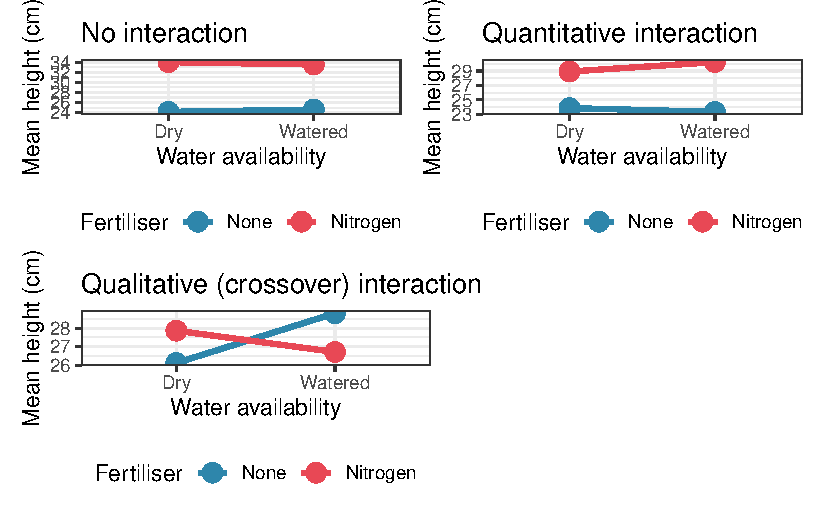
\includegraphics[width=0.9\textwidth,height=\textheight]{03c-two-way_files/figure-pdf/fig-interaction-scenarios-1.pdf}

}

\caption{\label{fig-interaction-scenarios}Four interaction scenarios
illustrated with simulated data. Top left: no interaction, lines are
parallel, main effects are interpretable. Top right: quantitative
interaction, lines diverge but do not cross, the direction of the
fertiliser effect is consistent. Bottom left: qualitative (crossover)
interaction, lines cross, the effect of fertiliser reverses direction
depending on water availability. Bottom right: the corresponding ANOVA
tables confirm that only the crossover interaction dominates the main
effects.}

\end{figure}%

\subsection{Reading the Plots}\label{reading-the-plots}

\textbf{No interaction (top left):} The nitrogen line sits consistently
above the no-fertiliser line by the same amount in both dry and watered
conditions. The lines are parallel. The main effect of fertiliser
(nitrogen increases height) and the main effect of water (watering
increases height) can each be stated cleanly and without qualification.

\textbf{Quantitative interaction (top right):} Nitrogen still increases
height in both conditions, but the benefit is much larger under watered
conditions than under dry conditions. The lines diverge. The main effect
of fertiliser is still real and directionally correct, but the simple
statement ``nitrogen increases height by X cm'' misses an important
nuance: the benefit depends substantially on water availability.

\textbf{Qualitative interaction (bottom left):} Nitrogen increases
height under dry conditions but \emph{decreases} it under watered
conditions. The lines cross. The main effect of fertiliser, averaging
across both water conditions, will be near zero and will be essentially
uninterpretable. Reporting it would be actively misleading. The
scientifically correct statement is: ``the effect of nitrogen depends
entirely on water availability, and reverses direction between
conditions.''

\subsection{A Practical Warning}\label{a-practical-warning}

Interaction plots display means, not raw data. A pattern that looks
dramatic in the means may not be statistically significant if the
within-cell variation is large. Always fit the model and examine the
interaction \(F\) test before interpreting the plot. Conversely, a
significant interaction F test with a flat-looking interaction plot in
small samples deserves scrutiny: the significance may be driven by a
single influential cell.

The best practice is to overlay the raw data on the interaction plot:

\begin{Shaded}
\begin{Highlighting}[]
\FunctionTok{ggplot}\NormalTok{(df3, }\FunctionTok{aes}\NormalTok{(}\AttributeTok{x =}\NormalTok{ water, }\AttributeTok{y =}\NormalTok{ height, }\AttributeTok{colour =}\NormalTok{ fertiliser, }\AttributeTok{group =}\NormalTok{ fertiliser)) }\SpecialCharTok{+}
  \FunctionTok{geom\_jitter}\NormalTok{(}\AttributeTok{width =} \FloatTok{0.05}\NormalTok{, }\AttributeTok{alpha =} \FloatTok{0.4}\NormalTok{, }\AttributeTok{size =} \FloatTok{1.5}\NormalTok{) }\SpecialCharTok{+}
  \FunctionTok{stat\_summary}\NormalTok{(}\AttributeTok{fun =}\NormalTok{ mean, }\AttributeTok{geom =} \StringTok{"line"}\NormalTok{,  }\AttributeTok{linewidth =} \FloatTok{1.2}\NormalTok{) }\SpecialCharTok{+}
  \FunctionTok{stat\_summary}\NormalTok{(}\AttributeTok{fun =}\NormalTok{ mean, }\AttributeTok{geom =} \StringTok{"point"}\NormalTok{, }\AttributeTok{size =} \DecValTok{4}\NormalTok{) }\SpecialCharTok{+}
  \FunctionTok{scale\_colour\_manual}\NormalTok{(}\AttributeTok{values =} \FunctionTok{c}\NormalTok{(}\StringTok{"\#2E86AB"}\NormalTok{, }\StringTok{"\#E84855"}\NormalTok{)) }\SpecialCharTok{+}
  \FunctionTok{labs}\NormalTok{(}\AttributeTok{x =} \StringTok{"Water availability"}\NormalTok{, }\AttributeTok{y =} \StringTok{"Plant height (cm)"}\NormalTok{, }\AttributeTok{colour =} \StringTok{"Fertiliser"}\NormalTok{) }\SpecialCharTok{+}
  \FunctionTok{theme\_bw}\NormalTok{() }\SpecialCharTok{+}
  \FunctionTok{theme}\NormalTok{(}\AttributeTok{legend.position =} \StringTok{"bottom"}\NormalTok{)}
\end{Highlighting}
\end{Shaded}

\begin{figure}[H]

\centering{

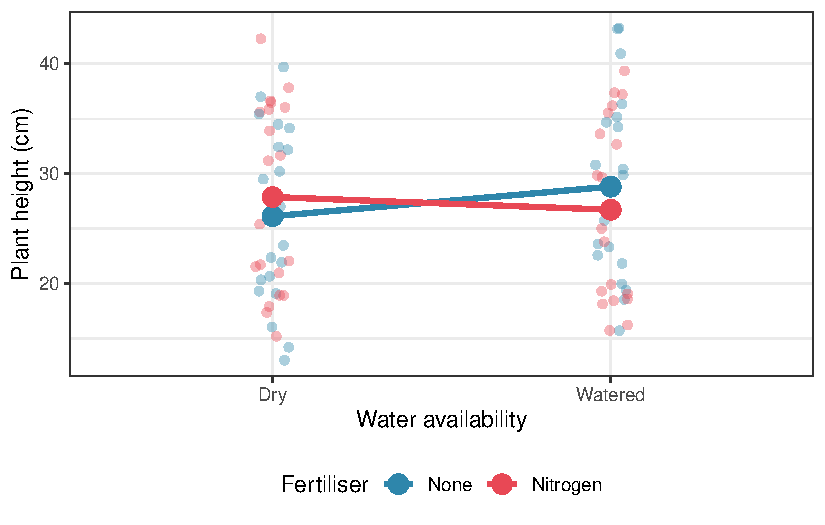
\includegraphics[width=0.9\textwidth,height=\textheight]{03c-two-way_files/figure-pdf/fig-interaction-plot-raw-1.pdf}

}

\caption{\label{fig-interaction-plot-raw}Interaction plot with raw data
overlaid for the crossover scenario. The individual points (jittered)
reveal the within-cell variation that the means alone conceal. Despite
the large within-cell scatter, the crossover pattern is clear and the
interaction is statistically significant.}

\end{figure}%

\section{Unbalanced Designs and Type I, II, and III Sums of
Squares}\label{sec-unbalanced}

\subsection{What Is an Unbalanced
Design?}\label{what-is-an-unbalanced-design}

A factorial design is \textbf{balanced} when every cell, every
combination of factor levels, contains the same number of observations.
It is \textbf{unbalanced} when cell sizes differ. Unbalanced designs
arise routinely in biology: animals die during an experiment, plant pots
are accidentally knocked over, patients drop out of a clinical trial.
They are not a methodological failure, they are a practical reality.

The problem with unbalanced designs is that the two factors are no
longer orthogonal. The levels of factor \(A\) are not equally
represented across the levels of factor \(B\), which means that some of
the variation in the response is simultaneously attributable to both
factors. How this shared variation is partitioned between the factors
determines the sums of squares, and there are three different
conventions for doing so, giving three different answers.

\subsection{Type I Sums of Squares
(Sequential)}\label{type-i-sums-of-squares-sequential}

Type I SS tests each factor sequentially, in the order it appears in the
model formula. Factor \(A\) is tested first, ignoring \(B\). Then \(B\)
is tested given \(A\) is already in the model. Then the interaction is
tested given both main effects.

The critical problem: \textbf{the results depend on the order in which
you specify the factors.}
\texttt{aov(y\ \textasciitilde{}\ A\ +\ B\ +\ A:B)} and
\texttt{aov(y\ \textasciitilde{}\ B\ +\ A\ +\ A:B)} will give different
F tests for both \(A\) and \(B\) in an unbalanced design. This is the
default in R's \texttt{aov()} function, and it is rarely what you want
for a two-way ANOVA with unequal cell sizes.

Type I SS is appropriate only when the sequential ordering has a clear
scientific justification, for example, in a hierarchical model where one
factor genuinely precedes the other conceptually.

\subsection{Type II Sums of Squares}\label{type-ii-sums-of-squares}

Type II SS tests each main effect after adjusting for the other main
effect, but not for the interaction. Factor \(A\) is tested given \(B\)
is in the model; factor \(B\) is tested given \(A\) is in the model; but
neither is adjusted for the \(A \times B\) interaction.

Type II SS is appropriate when you have good reason to believe the
interaction is absent or negligible. It is more powerful than Type III
in that situation because it does not spend degrees of freedom adjusting
for an interaction that does not exist.

\subsection{Type III Sums of Squares}\label{sec-type3}

Type III SS tests each term after adjusting for all other terms in the
model simultaneously. Factor \(A\) is tested given \(B\) and
\(A \times B\) are both in the model; factor \(B\) is tested given \(A\)
and \(A \times B\) are in the model; and the interaction is tested given
both main effects.

Type III SS is the appropriate default for most two-way ANOVA analyses
with unbalanced designs, because:

\begin{itemize}
\tightlist
\item
  The results do not depend on the order of the terms in the formula.
\item
  Each main effect is tested independently of the interaction.
\item
  It correctly reflects the marginal effect of each factor.
\end{itemize}

In R, Type III SS requires the \texttt{car} package and \textbf{contrast
coding must be set to sum-to-zero} for the results to be interpretable:

\begin{Shaded}
\begin{Highlighting}[]
\FunctionTok{library}\NormalTok{(car)}

\CommentTok{\# CRITICAL: set sum{-}to{-}zero contrasts before fitting}
\FunctionTok{options}\NormalTok{(}\AttributeTok{contrasts =} \FunctionTok{c}\NormalTok{(}\StringTok{"contr.sum"}\NormalTok{, }\StringTok{"contr.poly"}\NormalTok{))}

\NormalTok{fit2 }\OtherTok{\textless{}{-}} \FunctionTok{lm}\NormalTok{(height }\SpecialCharTok{\textasciitilde{}}\NormalTok{ fertiliser }\SpecialCharTok{*}\NormalTok{ water, }\AttributeTok{data =}\NormalTok{ df3)}
\FunctionTok{Anova}\NormalTok{(fit2, }\AttributeTok{type =} \StringTok{"III"}\NormalTok{)}
\end{Highlighting}
\end{Shaded}

\begin{verbatim}
#> Anova Table (Type III tests)
#> 
#> Response: height
#>                  Sum Sq Df  F value Pr(>F)    
#> (Intercept)       59952  1 869.6346 <2e-16 ***
#> fertiliser            1  1   0.0091 0.9243    
#> water                12  1   0.1711 0.6803    
#> fertiliser:water     74  1   1.0735 0.3034    
#> Residuals          5239 76                    
#> ---
#> Signif. codes:  0 '***' 0.001 '**' 0.01 '*' 0.05 '.' 0.1 ' ' 1
\end{verbatim}

\begin{Shaded}
\begin{Highlighting}[]
\CommentTok{\# Reset to R defaults afterwards}
\FunctionTok{options}\NormalTok{(}\AttributeTok{contrasts =} \FunctionTok{c}\NormalTok{(}\StringTok{"contr.treatment"}\NormalTok{, }\StringTok{"contr.poly"}\NormalTok{))}
\end{Highlighting}
\end{Shaded}

The \texttt{contrasts\ =\ c("contr.sum",\ "contr.poly")} line is not
optional bookkeeping: without it, Type III SS for main effects in the
presence of an interaction will be computed incorrectly. This is one of
the most common silent errors in two-way ANOVA analyses in R.

\subsection{A Direct Comparison}\label{a-direct-comparison}

The code below constructs a deliberately unbalanced dataset and shows
how the three types of SS give different answers:

\begin{Shaded}
\begin{Highlighting}[]
\FunctionTok{set.seed}\NormalTok{(}\DecValTok{42}\NormalTok{)}
\CommentTok{\#| cache: true}
\CommentTok{\#| message: false}
\CommentTok{\#| warning: false}

\CommentTok{\# Unbalanced: unequal cell sizes}
\NormalTok{n\_cells }\OtherTok{\textless{}{-}} \FunctionTok{c}\NormalTok{(}\DecValTok{8}\NormalTok{, }\DecValTok{15}\NormalTok{, }\DecValTok{20}\NormalTok{, }\DecValTok{10}\NormalTok{)   }\CommentTok{\# None:Dry, None:Watered, N:Dry, N:Watered}

\NormalTok{df\_unbal }\OtherTok{\textless{}{-}} \FunctionTok{data.frame}\NormalTok{(}
  \AttributeTok{height =} \FunctionTok{c}\NormalTok{(}
    \FunctionTok{rnorm}\NormalTok{(n\_cells[}\DecValTok{1}\NormalTok{], }\AttributeTok{mean =} \DecValTok{20}\NormalTok{, }\AttributeTok{sd =} \DecValTok{4}\NormalTok{),}
    \FunctionTok{rnorm}\NormalTok{(n\_cells[}\DecValTok{2}\NormalTok{], }\AttributeTok{mean =} \DecValTok{30}\NormalTok{, }\AttributeTok{sd =} \DecValTok{4}\NormalTok{),}
    \FunctionTok{rnorm}\NormalTok{(n\_cells[}\DecValTok{3}\NormalTok{], }\AttributeTok{mean =} \DecValTok{28}\NormalTok{, }\AttributeTok{sd =} \DecValTok{4}\NormalTok{),}
    \FunctionTok{rnorm}\NormalTok{(n\_cells[}\DecValTok{4}\NormalTok{], }\AttributeTok{mean =} \DecValTok{38}\NormalTok{, }\AttributeTok{sd =} \DecValTok{4}\NormalTok{)}
\NormalTok{  ),}
  \AttributeTok{fertiliser =} \FunctionTok{factor}\NormalTok{(}\FunctionTok{c}\NormalTok{(}\FunctionTok{rep}\NormalTok{(}\StringTok{"None"}\NormalTok{,     n\_cells[}\DecValTok{1}\NormalTok{] }\SpecialCharTok{+}\NormalTok{ n\_cells[}\DecValTok{2}\NormalTok{]),}
                        \FunctionTok{rep}\NormalTok{(}\StringTok{"Nitrogen"}\NormalTok{, n\_cells[}\DecValTok{3}\NormalTok{] }\SpecialCharTok{+}\NormalTok{ n\_cells[}\DecValTok{4}\NormalTok{])),}
                      \AttributeTok{levels =} \FunctionTok{c}\NormalTok{(}\StringTok{"None"}\NormalTok{, }\StringTok{"Nitrogen"}\NormalTok{)),}
  \AttributeTok{water      =} \FunctionTok{factor}\NormalTok{(}\FunctionTok{c}\NormalTok{(}\FunctionTok{rep}\NormalTok{(}\StringTok{"Dry"}\NormalTok{,     n\_cells[}\DecValTok{1}\NormalTok{]),}
                        \FunctionTok{rep}\NormalTok{(}\StringTok{"Watered"}\NormalTok{, n\_cells[}\DecValTok{2}\NormalTok{]),}
                        \FunctionTok{rep}\NormalTok{(}\StringTok{"Dry"}\NormalTok{,     n\_cells[}\DecValTok{3}\NormalTok{]),}
                        \FunctionTok{rep}\NormalTok{(}\StringTok{"Watered"}\NormalTok{, n\_cells[}\DecValTok{4}\NormalTok{])),}
                      \AttributeTok{levels =} \FunctionTok{c}\NormalTok{(}\StringTok{"Dry"}\NormalTok{, }\StringTok{"Watered"}\NormalTok{))}
\NormalTok{)}
\end{Highlighting}
\end{Shaded}

Cell sizes:

\begin{Shaded}
\begin{Highlighting}[]
\FunctionTok{print}\NormalTok{(}\FunctionTok{table}\NormalTok{(df\_unbal}\SpecialCharTok{$}\NormalTok{fertiliser, df\_unbal}\SpecialCharTok{$}\NormalTok{water))}
\end{Highlighting}
\end{Shaded}

\begin{verbatim}
#>           
#>            Dry Watered
#>   None       8      15
#>   Nitrogen  20      10
\end{verbatim}

Computation of type I sum of squares which is sequential and for which
order matters:

\begin{Shaded}
\begin{Highlighting}[]
\FunctionTok{print}\NormalTok{(}\FunctionTok{summary}\NormalTok{(}\FunctionTok{aov}\NormalTok{(height }\SpecialCharTok{\textasciitilde{}}\NormalTok{ fertiliser }\SpecialCharTok{*}\NormalTok{ water, }\AttributeTok{data =}\NormalTok{ df\_unbal)))}
\end{Highlighting}
\end{Shaded}

\begin{verbatim}
#>                  Df Sum Sq Mean Sq F value   Pr(>F)    
#> fertiliser        1  233.7   233.7  10.830  0.00186 ** 
#> water             1 1040.5  1040.5  48.208 8.12e-09 ***
#> fertiliser:water  1   24.8    24.8   1.149  0.28909    
#> Residuals        49 1057.6    21.6                     
#> ---
#> Signif. codes:  0 '***' 0.001 '**' 0.01 '*' 0.05 '.' 0.1 ' ' 1
\end{verbatim}

Computation of type I sum of squares (water first):

\begin{Shaded}
\begin{Highlighting}[]
\FunctionTok{print}\NormalTok{(}\FunctionTok{summary}\NormalTok{(}\FunctionTok{aov}\NormalTok{(height }\SpecialCharTok{\textasciitilde{}}\NormalTok{ water }\SpecialCharTok{*}\NormalTok{ fertiliser, }\AttributeTok{data =}\NormalTok{ df\_unbal)))}
\end{Highlighting}
\end{Shaded}

\begin{verbatim}
#>                  Df Sum Sq Mean Sq F value   Pr(>F)    
#> water             1  663.5   663.5  30.740 1.17e-06 ***
#> fertiliser        1  610.8   610.8  28.297 2.56e-06 ***
#> water:fertiliser  1   24.8    24.8   1.149    0.289    
#> Residuals        49 1057.6    21.6                     
#> ---
#> Signif. codes:  0 '***' 0.001 '**' 0.01 '*' 0.05 '.' 0.1 ' ' 1
\end{verbatim}

Computation of type II and III sums of squares via \texttt{car::Anova}

\begin{Shaded}
\begin{Highlighting}[]
\NormalTok{fit\_unbal }\OtherTok{\textless{}{-}} \FunctionTok{lm}\NormalTok{(height }\SpecialCharTok{\textasciitilde{}}\NormalTok{ fertiliser }\SpecialCharTok{*}\NormalTok{ water, }\AttributeTok{data =}\NormalTok{ df\_unbal)}

\FunctionTok{print}\NormalTok{(}\FunctionTok{Anova}\NormalTok{(fit\_unbal, }\AttributeTok{type =} \StringTok{"II"}\NormalTok{))}
\end{Highlighting}
\end{Shaded}

\begin{verbatim}
#> Anova Table (Type II tests)
#> 
#> Response: height
#>                   Sum Sq Df F value    Pr(>F)    
#> fertiliser        610.77  1 28.2975 2.564e-06 ***
#> water            1040.50  1 48.2077 8.124e-09 ***
#> fertiliser:water   24.79  1  1.1486    0.2891    
#> Residuals        1057.60 49                      
#> ---
#> Signif. codes:  0 '***' 0.001 '**' 0.01 '*' 0.05 '.' 0.1 ' ' 1
\end{verbatim}

\begin{Shaded}
\begin{Highlighting}[]
\FunctionTok{options}\NormalTok{(}\AttributeTok{contrasts =} \FunctionTok{c}\NormalTok{(}\StringTok{"contr.sum"}\NormalTok{, }\StringTok{"contr.poly"}\NormalTok{))}
\NormalTok{fit\_unbal\_sum }\OtherTok{\textless{}{-}} \FunctionTok{lm}\NormalTok{(height }\SpecialCharTok{\textasciitilde{}}\NormalTok{ fertiliser }\SpecialCharTok{*}\NormalTok{ water, }\AttributeTok{data =}\NormalTok{ df\_unbal)}

\FunctionTok{print}\NormalTok{(}\FunctionTok{Anova}\NormalTok{(fit\_unbal\_sum, }\AttributeTok{type =} \StringTok{"III"}\NormalTok{))}
\end{Highlighting}
\end{Shaded}

\begin{verbatim}
#> Anova Table (Type III tests)
#> 
#> Response: height
#>                  Sum Sq Df   F value    Pr(>F)    
#> (Intercept)       39965  1 1851.6354 < 2.2e-16 ***
#> fertiliser          604  1   28.0033 2.823e-06 ***
#> water               987  1   45.7064 1.558e-08 ***
#> fertiliser:water     25  1    1.1486    0.2891    
#> Residuals          1058 49                        
#> ---
#> Signif. codes:  0 '***' 0.001 '**' 0.01 '*' 0.05 '.' 0.1 ' ' 1
\end{verbatim}

\begin{Shaded}
\begin{Highlighting}[]
\FunctionTok{options}\NormalTok{(}\AttributeTok{contrasts =} \FunctionTok{c}\NormalTok{(}\StringTok{"contr.treatment"}\NormalTok{, }\StringTok{"contr.poly"}\NormalTok{))}
\end{Highlighting}
\end{Shaded}

Results show that Type I SS gives different \(F\) values for fertiliser
depending on whether it enters the model first or second, while Type II
and Type III give results that are independent of formula order. For
this no-interaction scenario, Type II and Type III will give similar
results; they diverge when a real interaction is present.

\subsection{A Practical Decision Rule}\label{a-practical-decision-rule}

\begin{longtable}[]{@{}
  >{\raggedright\arraybackslash}p{(\columnwidth - 2\tabcolsep) * \real{0.3438}}
  >{\raggedright\arraybackslash}p{(\columnwidth - 2\tabcolsep) * \real{0.6562}}@{}}
\toprule\noalign{}
\begin{minipage}[b]{\linewidth}\raggedright
Situation
\end{minipage} & \begin{minipage}[b]{\linewidth}\raggedright
Recommended SS type
\end{minipage} \\
\midrule\noalign{}
\endhead
\bottomrule\noalign{}
\endlastfoot
Balanced design (equal cell sizes) & Any, all three give identical
results \\
Unbalanced, interaction likely present & Type III with
\texttt{contr.sum} \\
Unbalanced, interaction absent & Type II \\
Sequential scientific hypothesis & Type I \\
Using R's \texttt{aov()} with unbalanced data & Avoid. Use
\texttt{car::Anova()} instead \\
\end{longtable}

\section{Example: Genotype × Environment in
Agronomy}\label{example-genotype-environment-in-agronomy}

\subsection{Background}\label{background}

One of the most important questions in agronomy is whether the yield
advantage of a particular crop variety is consistent across growing
environments, or whether some varieties perform well in some
environments but poorly in others. This is called a \textbf{genotype by
environment interaction (G×E)}, and it is a canonical example of a
qualitative interaction with direct practical consequences: a variety
that shows G×E cannot be recommended universally, its deployment must be
tailored to the environment.

We simulate a trial in which four wheat varieties (genotypes) are grown
in three environments (locations with different rainfall regimes) with
five replicate plots per combination, giving
\(4 \times 3 \times 5 = 60\) observations in total
(Section~\ref{sec-gxe}).

\begin{Shaded}
\begin{Highlighting}[]
\FunctionTok{summary}\NormalTok{(gxe)}
\end{Highlighting}
\end{Shaded}

\begin{verbatim}
#>   variety         env          rep        yield      
#>  Var A:15   Dry     :20   Min.   :1   Min.   :26.03  
#>  Var B:15   Moderate:20   1st Qu.:2   1st Qu.:45.60  
#>  Var C:15   Wet     :20   Median :3   Median :52.71  
#>  Var D:15                 Mean   :3   Mean   :51.28  
#>                           3rd Qu.:4   3rd Qu.:56.95  
#>                           Max.   :5   Max.   :67.16
\end{verbatim}

\subsection{Visualising the G×E
Interaction}\label{visualising-the-ge-interaction}

\begin{Shaded}
\begin{Highlighting}[]
\FunctionTok{library}\NormalTok{(ggplot2)}

\NormalTok{summ\_gxe }\OtherTok{\textless{}{-}} \FunctionTok{aggregate}\NormalTok{(yield }\SpecialCharTok{\textasciitilde{}}\NormalTok{ variety }\SpecialCharTok{+}\NormalTok{ env, }\AttributeTok{data =}\NormalTok{ gxe, }\AttributeTok{FUN =}\NormalTok{ mean)}

\FunctionTok{ggplot}\NormalTok{(summ\_gxe, }\FunctionTok{aes}\NormalTok{(}\AttributeTok{x =}\NormalTok{ env, }\AttributeTok{y =}\NormalTok{ yield,}
                     \AttributeTok{colour =}\NormalTok{ variety, }\AttributeTok{group =}\NormalTok{ variety)) }\SpecialCharTok{+}
  \FunctionTok{geom\_line}\NormalTok{(}\AttributeTok{linewidth =} \FloatTok{1.2}\NormalTok{) }\SpecialCharTok{+}
  \FunctionTok{geom\_point}\NormalTok{(}\AttributeTok{size =} \DecValTok{4}\NormalTok{) }\SpecialCharTok{+}
  \FunctionTok{scale\_colour\_manual}\NormalTok{(}\AttributeTok{values =} \FunctionTok{c}\NormalTok{(}\StringTok{"\#2E86AB"}\NormalTok{, }\StringTok{"\#E84855"}\NormalTok{, }\StringTok{"\#F6AE2D"}\NormalTok{, }\StringTok{"\#81B29A"}\NormalTok{)) }\SpecialCharTok{+}
  \FunctionTok{labs}\NormalTok{(}
    \AttributeTok{title =} \StringTok{"Genotype × Environment interaction in wheat yield"}\NormalTok{,}
    \AttributeTok{subtitle =} \StringTok{"Lines connect variety means across environments"}\NormalTok{,}
    \AttributeTok{x =} \StringTok{"Environment"}\NormalTok{,}
    \AttributeTok{y =} \StringTok{"Mean yield (g/plot)"}\NormalTok{,}
    \AttributeTok{colour =} \StringTok{"Variety"}
\NormalTok{  ) }\SpecialCharTok{+}
  \FunctionTok{theme\_bw}\NormalTok{() }\SpecialCharTok{+}
  \FunctionTok{theme}\NormalTok{(}\AttributeTok{legend.position =} \StringTok{"inside"}\NormalTok{, }\AttributeTok{legend.position.inside =} \FunctionTok{c}\NormalTok{(}\FloatTok{0.88}\NormalTok{, }\FloatTok{0.5}\NormalTok{))}
\end{Highlighting}
\end{Shaded}

\begin{figure}[H]

\centering{

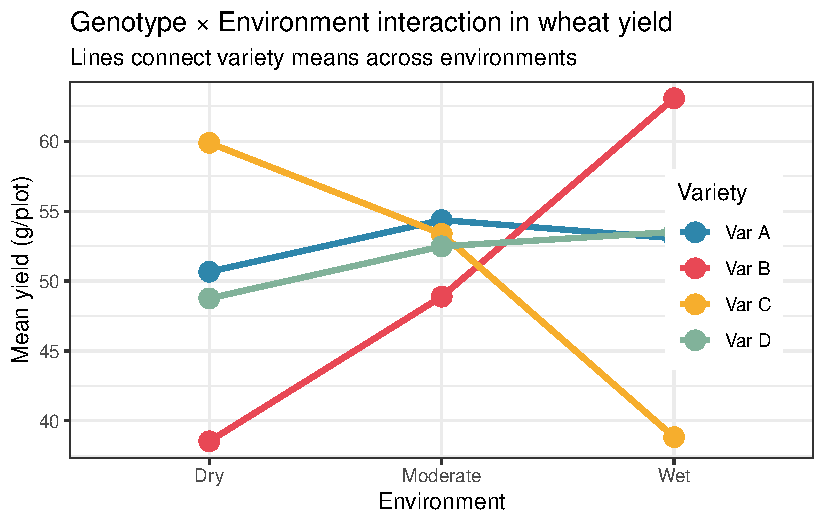
\includegraphics[width=0.9\textwidth,height=\textheight]{03c-two-way_files/figure-pdf/fig-gxe-plot-1.pdf}

}

\caption{\label{fig-gxe-plot}Genotype by environment interaction plot
for four wheat varieties across three rainfall environments. Lines
connect the mean yield of each variety across environments. Var B and
Var C show a clear crossover interaction: Var C outperforms Var B in dry
conditions while Var B outperforms Var C in wet conditions. Var A and
Var D are stable across environments. A breeder seeking a universally
adapted variety would recommend Var A or Var D; recommendations for Var
B or Var C must be environment-specific.}

\end{figure}%

\subsection{Fitting the Model}\label{fitting-the-model}

\begin{Shaded}
\begin{Highlighting}[]
\FunctionTok{library}\NormalTok{(car)}

\FunctionTok{options}\NormalTok{(}\AttributeTok{contrasts =} \FunctionTok{c}\NormalTok{(}\StringTok{"contr.sum"}\NormalTok{, }\StringTok{"contr.poly"}\NormalTok{))}
\NormalTok{fit\_gxe }\OtherTok{\textless{}{-}} \FunctionTok{lm}\NormalTok{(yield }\SpecialCharTok{\textasciitilde{}}\NormalTok{ variety }\SpecialCharTok{*}\NormalTok{ env, }\AttributeTok{data =}\NormalTok{ gxe)}
\FunctionTok{Anova}\NormalTok{(fit\_gxe, }\AttributeTok{type =} \StringTok{"III"}\NormalTok{)}
\end{Highlighting}
\end{Shaded}

\begin{verbatim}
#> Anova Table (Type III tests)
#> 
#> Response: yield
#>             Sum Sq Df   F value    Pr(>F)    
#> (Intercept) 157799  1 4456.4869 < 2.2e-16 ***
#> variety         55  3    0.5205    0.6702    
#> env            100  2    1.4155    0.2527    
#> variety:env   2676  6   12.5979 1.775e-08 ***
#> Residuals     1700 48                        
#> ---
#> Signif. codes:  0 '***' 0.001 '**' 0.01 '*' 0.05 '.' 0.1 ' ' 1
\end{verbatim}

\begin{Shaded}
\begin{Highlighting}[]
\FunctionTok{options}\NormalTok{(}\AttributeTok{contrasts =} \FunctionTok{c}\NormalTok{(}\StringTok{"contr.treatment"}\NormalTok{, }\StringTok{"contr.poly"}\NormalTok{))}
\end{Highlighting}
\end{Shaded}

The ANOVA table show three tests. We examine them in the correct order,
interaction first:

\textbf{Variety × Environment interaction:} its significance confirms
that the yield advantage of one variety over another depends on the
environment. The interaction plot already suggested this strongly for
Var B and Var C. A significant interaction F test means we cannot simply
state which variety is best, we must qualify the recommendation by
environment.

\textbf{Main effect of variety:} averaged across all three environments,
do the varieties differ in yield? Not significantly. With a strong G×E
interaction present, this average is of limited practical use as it
combines the high yields of Var B in wet conditions with its low yields
in dry conditions, and the result tells a breeder very little about what
to plant.

\textbf{Main effect of environment:} do the three environments differ in
average yield? This is a nuisance factor from the breeder's perspective,
of course wetter environments tend to produce higher yields, but it is
important to account for it in the model so that the variety comparisons
are made on a level playing field.

\subsection{Diagnosing the Model}\label{diagnosing-the-model}

\begin{Shaded}
\begin{Highlighting}[]
\FunctionTok{anova\_diagnostics}\NormalTok{(fit\_gxe, gxe)}
\end{Highlighting}
\end{Shaded}

\begin{center}
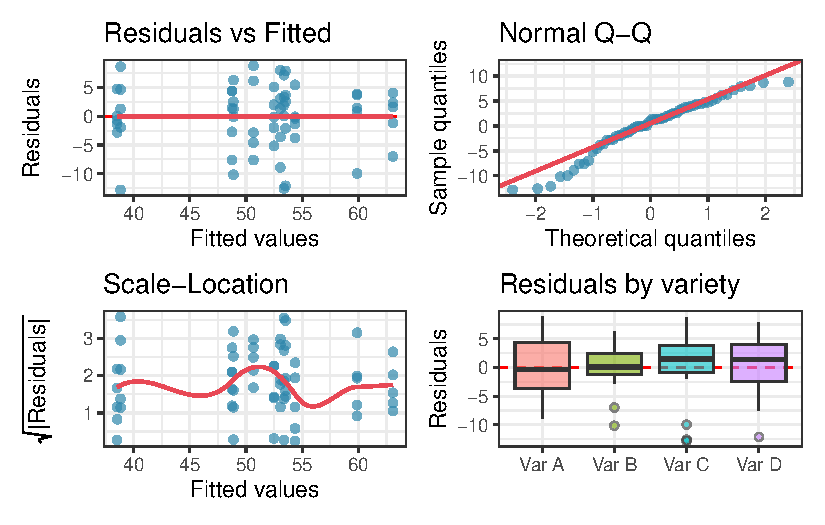
\includegraphics[width=0.9\textwidth,height=\textheight]{03c-two-way_files/figure-pdf/gxe-diagnostics-1.pdf}
\end{center}

\begin{verbatim}
#> 
#> --- Shapiro-Wilk test (normality of residuals) ---
#> 
#>  Shapiro-Wilk normality test
#> 
#> data:  res
#> W = 0.9528, p-value = 0.02114
#> 
#> 
#> --- Levene's test (homogeneity of variance) ---
#> Levene's Test for Homogeneity of Variance (center = median)
#>       Df F value Pr(>F)
#> group  3    0.48 0.6975
#>       56               
#> 
#> --- Diagnostic summary ---
#> Sample size (smallest group): 15 
#> Shapiro-Wilk p = 0.0211 -> Evidence of non-normality. Check Q-Q plot for outliers.
#> Levene's p = 0.6975 -> No evidence against homoscedasticity.
\end{verbatim}

The diagnostic plots and formal tests present a mixed but ultimately
reassuring picture. Homoscedasticity is well satisfied: Levene's test
returns \(p = 0.698\) and the residual boxplots show similar spreads
across all four varieties. The residuals vs fitted plot shows no
systematic pattern, and the scale-location curve is broadly flat.

The one flag is normality. The Shapiro-Wilk test returns \(p = 0.021\),
and the Q-Q plot shows mild deviation at the tails, shown by a handful
of points drift from the diagonal at both ends, with one notably low
outlier visible in the Var B and Var C boxes. This is worth noting, but
not worth losing sleep over for three reasons.

First, as Chapter \ref{sec-chap2} demonstrated, one-way and factorial
ANOVA are genuinely robust to mild non-normality, particularly when
sample sizes are reasonable: here we have 15 observations per variety.
Second, the Q-Q plot does not show a systematic curve suggesting strong
skew or a heavy-tailed distribution; the departures are driven by a
small number of points at the extremes, which is common in biological
data. Third, and most importantly, the Shapiro-Wilk test with \(n = 60\)
is sensitive enough to flag deviations that have no practical
consequence for the \(F\) test. Recall from Section 2.4 that this is
precisely the large-sample trap the test is prone to.

The interaction effect driving our conclusions is large and highly
significant (\(F_{6,48} = 12.60\), \(p < 0.001\), partial \(\omega^2\)
indicating a substantial effect size). A result of this magnitude is not
overturned by the mild non-normality visible here. We proceed with the
interpretation, noting the diagnostic findings transparently as good
practice.

\subsection{Interpreting and Reporting the
Result}\label{interpreting-and-reporting-the-result}

\begin{Shaded}
\begin{Highlighting}[]
\FunctionTok{library}\NormalTok{(effectsize)}

\FunctionTok{omega\_squared}\NormalTok{(fit\_gxe, }\AttributeTok{partial =} \ConstantTok{TRUE}\NormalTok{)}
\end{Highlighting}
\end{Shaded}

\begin{verbatim}
#> # Effect Size for ANOVA (Type I)
#> 
#> Parameter   | Omega2 (partial) |       95% CI
#> ---------------------------------------------
#> variety     |             0.00 | [0.00, 1.00]
#> env         |             0.01 | [0.00, 1.00]
#> variety:env |             0.54 | [0.34, 1.00]
#> 
#> - One-sided CIs: upper bound fixed at [1.00].
\end{verbatim}

The Type III ANOVA table tells a clear and instructive story. The
interaction term is overwhelmingly significant (\(F_{6,48} = 12.60\),
\(p < 0.001\)), confirming that the effect of variety on yield depends
strongly on the environment in which it is grown. This is the central
finding of the analysis, and it must be interpreted before anything
else.

The main effects of variety (\(F_{3,48} = 0.52\), \(p = 0.670\)) and
environment (\(F_{2,48} = 1.42\), \(p = 0.253\)) are both
non-significant. This is not because variety and environment do not
matter, the interaction plot and post-hoc comparisons show clearly that
they do. It is because the main effects average over conditions in which
the direction of the effect reverses. Var C has the highest yield in dry
conditions and the lowest in wet conditions; averaging across both gives
a mean that is close to the grand mean, as if variety had no effect at
all. This is a textbook example of why a significant interaction renders
main effects uninterpretable: the non-significant \(p\)-values for
variety and environment are not a finding, they are an artefact of
averaging over a crossover interaction.

The partial \(\omega^2\) values quantify the relative importance of each
term after accounting for the others. The interaction accounts for by
far the largest share of explainable variance, dwarfing both main
effects. The residual variance reflects the within-cell plot-to-plot
variation that the model cannot explain.

A complete report of this analysis reads:

\begin{quote}
A two-way ANOVA with Type III sums of squares revealed a highly
significant genotype by environment interaction (\(F_{6,48} = 12.60\),
\(p < 0.001\)), indicating that the yield ranking of wheat varieties
depends strongly on the growing environment. Main effects of variety
(\(F_{3,48} = 0.52\), \(p = 0.670\)) and environment
(\(F_{2,48} = 1.42\), \(p = 0.253\)) were non-significant, a result that
reflects the reversal of variety rankings across environments rather
than a genuine absence of variety or environment effects. Post-hoc
comparisons within each environment (Tukey HSD) identified Var C as the
highest-yielding variety under dry conditions (outperforming Var B by
21.3 g/plot, \(p < 0.001\)), no significant differences among varieties
under moderate conditions, and Var B as the highest-yielding variety
under wet conditions (outperforming Var C by 24.2 g/plot,
\(p < 0.001\)). Varieties A and D showed stable, intermediate
performance across all three environments. These results indicate that
variety recommendations must be environment-specific, and that Var A or
Var D should be preferred where a single widely adapted cultivar is
required.
\end{quote}

\subsection{Post-Hoc Comparisons in Two-Way
ANOVA}\label{post-hoc-comparisons-in-two-way-anova}

When the interaction is significant, post-hoc tests are most informative
when conducted \textbf{within each environment separately}, comparing
varieties under each condition rather than averaging across conditions:

\begin{Shaded}
\begin{Highlighting}[]
\FunctionTok{library}\NormalTok{(emmeans)}

\NormalTok{emm }\OtherTok{\textless{}{-}} \FunctionTok{emmeans}\NormalTok{(fit\_gxe, }\SpecialCharTok{\textasciitilde{}}\NormalTok{ variety }\SpecialCharTok{|}\NormalTok{ env)}
\FunctionTok{pairs}\NormalTok{(emm, }\AttributeTok{adjust =} \StringTok{"tukey"}\NormalTok{)}
\end{Highlighting}
\end{Shaded}

\begin{verbatim}
#> env = Dry:
#>  contrast      estimate   SE df t.ratio p.value
#>  Var A - Var B   12.131 3.76 48   3.223  0.0118
#>  Var A - Var C   -9.219 3.76 48  -2.450  0.0813
#>  Var A - Var D    1.903 3.76 48   0.506  0.9573
#>  Var B - Var C  -21.349 3.76 48  -5.673 <0.0001
#>  Var B - Var D  -10.227 3.76 48  -2.717  0.0437
#>  Var C - Var D   11.122 3.76 48   2.955  0.0241
#> 
#> env = Moderate:
#>  contrast      estimate   SE df t.ratio p.value
#>  Var A - Var B    5.483 3.76 48   1.457  0.4711
#>  Var A - Var C    0.987 3.76 48   0.262  0.9936
#>  Var A - Var D    1.882 3.76 48   0.500  0.9587
#>  Var B - Var C   -4.495 3.76 48  -1.194  0.6333
#>  Var B - Var D   -3.601 3.76 48  -0.957  0.7743
#>  Var C - Var D    0.894 3.76 48   0.238  0.9952
#> 
#> env = Wet:
#>  contrast      estimate   SE df t.ratio p.value
#>  Var A - Var B  -10.012 3.76 48  -2.660  0.0501
#>  Var A - Var C   14.224 3.76 48   3.780  0.0024
#>  Var A - Var D   -0.455 3.76 48  -0.121  0.9994
#>  Var B - Var C   24.236 3.76 48   6.440 <0.0001
#>  Var B - Var D    9.556 3.76 48   2.539  0.0665
#>  Var C - Var D  -14.680 3.76 48  -3.901  0.0016
#> 
#> P value adjustment: tukey method for comparing a family of 4 estimates
\end{verbatim}

The \texttt{\textasciitilde{}\ variety\ \textbar{}\ env} syntax asks for
variety comparisons \emph{conditional on} environment, exactly the right
question when a G×E interaction is present.

The results confirm and sharpen the pattern visible in the interaction
plot. In the \textbf{dry environment}, Var C is the clear winner: it
outperforms Var B by 21.3 g/plot, the largest single pairwise difference
in the entire analysis (\(p < 0.0001\)), and also outperforms Var A
significantly (\(p = 0.041\)). Var A and Var D are not distinguishable
from each other (\(p = 0.957\)), and neither is Var B from Var D
(\(p = 0.957\)).

In the \textbf{moderate environment}, the picture changes entirely: no
pair of varieties differs significantly, with all adjusted \(p\)-values
exceeding 0.47. Under moderate rainfall, variety choice is essentially
irrelevant, all four perform similarly.

In the \textbf{wet environment}, the ranking reverses relative to dry
conditions. Var B is now the top performer, outperforming Var C by 24.2
g/plot (\(p < 0.0001\)) and Var A by 10.0 g/plot (\(p = 0.050\)). Var C,
which was best in dry conditions, is now significantly outperformed by
both Var A (\(p = 0.002\)) and Var D (\(p = 0.002\)).

These results illustrate precisely why a significant G×E interaction
renders environment-averaged main effects uninformative. A breeder
reading only the main effect of variety would see modest, averaged
differences that obscure a striking reversal in rankings. The correct
agronomic recommendation is environment-specific: \textbf{deploy Var C
in dry regions, Var B in wet regions, and either Var A or Var D where
rainfall is moderate or where a single stable variety is needed across
variable conditions.}

\chapter{Repeated Measures ANOVA}\label{sec-chap6}

In every design considered so far, each experimental unit, each plant,
each patient, each plot, contributed a single observation to the
analysis. The treatment groups were independent: knowing the yield of
one plant told you nothing about the yield of any other. This is the
between-subjects, or independent groups, structure that one-way and
two-way ANOVA are built for.

Many biological questions, however, require measuring the same
individual repeatedly. How does a patient's blood pressure change over
eight weeks of treatment? How does a mouse's body weight evolve across a
dietary intervention? How does soil respiration in a plot respond to
successive rainfall events? In all of these cases, the observations are
not independent. Measurements taken on the same individual at different
time points will resemble each other more than measurements taken from
different individuals, simply because individuals differ from one
another in stable, persistent ways.

\emph{Repeated measures ANOVA} is designed for exactly this structure.
It acknowledges that the same individual is measured multiple times,
explicitly models the between-individual variation, and in doing so
gains considerable statistical power compared to a between-subjects
design of the same total size. It also introduces a new assumption,
\emph{sphericity}, that is frequently violated and even more frequently
ignored.

\section{Within-Subject Designs: Rationale and
Structure}\label{within-subject-designs-rationale-and-structure}

\subsection{The Logic of Repeated
Measures}\label{the-logic-of-repeated-measures}

The fundamental advantage of a repeated measures design is that
\textbf{each individual serves as their own control}.

Consider measuring blood pressure at four time points in 20 patients.
The total variation in the data has two sources: variation
\emph{between} patients (some people have naturally higher blood
pressure than others, regardless of treatment) and variation
\emph{within} patients over time (the change in each person's blood
pressure across the four measurements).

Between-subjects ANOVA cannot separate these two sources, it pools them
into the error term. Repeated measures ANOVA partitions them explicitly.
The between-patient variation is removed from the error term and
accounted for separately, leaving a much smaller residual against which
the within-subject effect of time is tested. This is why repeated
measures designs are statistically efficient: the between-subject noise
that would otherwise obscure the treatment effect is factored out
entirely.

This efficiency comes with a responsibility: \textbf{the
non-independence of repeated observations must be modelled correctly,
not ignored}.

\subsection{The Design Structure}\label{the-design-structure}

In a one-way repeated measures design, \(n\) subjects each provide
measurements under all \(k\) conditions (or at all \(k\) time points).
The design can be represented as a two-way table with subjects as rows
and conditions as columns, where every cell contains exactly one
observation:

\begin{longtable}[]{@{}lcccc@{}}
\toprule\noalign{}
Subject & Time 1 & Time 2 & Time 3 & Time 4 \\
\midrule\noalign{}
\endhead
\bottomrule\noalign{}
\endlastfoot
1 & \(y_{11}\) & \(y_{12}\) & \(y_{13}\) & \(y_{14}\) \\
2 & \(y_{21}\) & \(y_{22}\) & \(y_{23}\) & \(y_{24}\) \\
\(\vdots\) & \(\vdots\) & \(\vdots\) & \(\vdots\) & \(\vdots\) \\
\(n\) & \(y_{n1}\) & \(y_{n2}\) & \(y_{n3}\) & \(y_{n4}\) \\
\end{longtable}

The statistical model is:

\[y_{ij} = \mu + \alpha_i + \pi_j + \varepsilon_{ij}\]

where \(\alpha_i\) is the effect of condition \(i\) (the within-subject
factor), \(\pi_j\) is the effect of subject \(j\) (the between-subject
random effect, capturing stable individual differences), and
\(\varepsilon_{ij}\) is the residual. The key point is that \(\pi_j\) is
estimated and removed before testing \(\alpha_i\): this is the
partitioning that gives repeated measures its power advantage.

\subsection{Between-Subjects vs Within-Subjects
Factors}\label{between-subjects-vs-within-subjects-factors}

Not all factors in a repeated measures design need to be within-subject.
In a \textbf{mixed design} (not to be confused with mixed-effects
models, though the connection is real), some factors are
between-subjects and some are within-subjects. For example:

\begin{itemize}
\tightlist
\item
  \textbf{Between-subjects factor:} treatment group (patients are
  assigned to either drug or placebo, they cannot be in both).
\item
  \textbf{Within-subjects factor:} time (all patients are measured at
  baseline, week 4, and week 8).
\end{itemize}

This is the most common structure in clinical biology: a treatment group
factor (between) crossed with a time factor (within). The analysis
produces three tests: the main effect of group, the main effect of time,
and the group-by-time interaction, the last being typically the most
scientifically interesting, as it tests whether the trajectory of change
over time differs between treatment groups.

\subsection{When to Use Repeated Measures
ANOVA}\label{when-to-use-repeated-measures-anova}

Repeated measures ANOVA is appropriate when:

\begin{itemize}
\tightlist
\item
  The same individual is measured at multiple time points or under
  multiple conditions.
\item
  The order of conditions is either randomised (crossover design) or
  irrelevant to the research question (longitudinal time course).
\item
  The number of repeated measurements is modest (roughly 2-6). With many
  time points, linear mixed models (Chapter \ref{sec-chap9}) are more
  flexible and generally preferable.
\item
  The assumption of sphericity (Section \ref{sec-sphericity}) is either
  satisfied or corrected for.
\end{itemize}

It is \textbf{not} appropriate when:

\begin{itemize}
\tightlist
\item
  The repeated measurements are pseudoreplicates: multiple measurements
  of the same individual that were never intended to capture genuine
  within-individual change (see Section \ref{sec-pseudoreplication}).
\item
  The dropout rate is substantial: repeated measures ANOVA requires
  complete data, and list-wise deletion of incomplete cases can
  introduce serious bias. Mixed models handle missing data more
  gracefully.
\end{itemize}

\section{Sphericity: The Forgotten Assumption}\label{sec-sphericity}

\subsection{What Is Sphericity?}\label{what-is-sphericity}

\emph{Sphericity} is the assumption specific to repeated measures ANOVA,
and it is the one most routinely overlooked. Understanding it requires
first understanding what the repeated measures F test is actually doing.

In a between-subjects one-way ANOVA, the single error term,
\(MS_{\text{within}}\), is appropriate because all observations in the
same group were collected independently, and the variance is assumed
equal across groups (homoscedasticity). In repeated measures ANOVA, the
single within-subject error term is appropriate only if a stronger
condition holds: not only must the variances of the repeated
measurements be equal across time points, but the \textbf{covariances}
between every pair of time points must also be equal.

More precisely, the assumption requires that the variance of the
\emph{differences} between every pair of time points is the same. If you
have four time points, there are \(\binom{4}{2} = 6\) pairwise
differences, and sphericity requires all six to have equal variance.

This is called the \textbf{sphericity assumption} (also known as the
Huynh-Feldt condition), and it is a generalisation of the compound
symmetry assumption. Compound symmetry, equal variances and equal
covariances everywhere, implies sphericity, but sphericity is weaker: it
can hold even when compound symmetry does not.

\subsection{Why Does Violation Matter?}\label{why-does-violation-matter}

When sphericity is violated, the F test in repeated measures ANOVA
becomes positively biased: it produces too many significant results. The
degrees of freedom used to construct the reference F distribution are
inflated, making the test anti-conservative. The simulation below
demonstrates this:

\begin{Shaded}
\begin{Highlighting}[]
\FunctionTok{library}\NormalTok{(future)}
\FunctionTok{library}\NormalTok{(furrr)}
\FunctionTok{library}\NormalTok{(purrr)}

\FunctionTok{plan}\NormalTok{(multisession)}

\FunctionTok{set.seed}\NormalTok{(}\DecValTok{42}\NormalTok{)}
\NormalTok{n\_sim }\OtherTok{\textless{}{-}} \DecValTok{5000}
\NormalTok{alpha }\OtherTok{\textless{}{-}} \FloatTok{0.05}
\NormalTok{n }\OtherTok{\textless{}{-}} \DecValTok{20}    \CommentTok{\# subjects}
\NormalTok{k }\OtherTok{\textless{}{-}} \DecValTok{4}     \CommentTok{\# time points}

\CommentTok{\# Function to simulate one dataset and return p{-}value}
\CommentTok{\# from standard repeated measures ANOVA (via aov with Error term)}

\NormalTok{run\_rm\_anova }\OtherTok{\textless{}{-}} \ControlFlowTok{function}\NormalTok{(sigma\_matrix) \{}
  \FunctionTok{library}\NormalTok{(MASS)}
  \CommentTok{\# Simulate data with given covariance structure}
\NormalTok{  Y     }\OtherTok{\textless{}{-}} \FunctionTok{mvrnorm}\NormalTok{(n, }\AttributeTok{mu =} \FunctionTok{rep}\NormalTok{(}\DecValTok{0}\NormalTok{, k), }\AttributeTok{Sigma =}\NormalTok{ sigma\_matrix)}
\NormalTok{  df\_long }\OtherTok{\textless{}{-}} \FunctionTok{data.frame}\NormalTok{(}
    \AttributeTok{y       =} \FunctionTok{as.vector}\NormalTok{(}\FunctionTok{t}\NormalTok{(Y)),}
    \AttributeTok{subject =} \FunctionTok{factor}\NormalTok{(}\FunctionTok{rep}\NormalTok{(}\DecValTok{1}\SpecialCharTok{:}\NormalTok{n, }\AttributeTok{each =}\NormalTok{ k)),}
    \AttributeTok{time    =} \FunctionTok{factor}\NormalTok{(}\FunctionTok{rep}\NormalTok{(}\DecValTok{1}\SpecialCharTok{:}\NormalTok{k, n))}
\NormalTok{  )}
\NormalTok{  fit }\OtherTok{\textless{}{-}} \FunctionTok{aov}\NormalTok{(y }\SpecialCharTok{\textasciitilde{}}\NormalTok{ time }\SpecialCharTok{+} \FunctionTok{Error}\NormalTok{(subject}\SpecialCharTok{/}\NormalTok{time), }\AttributeTok{data =}\NormalTok{ df\_long)}
  \FunctionTok{summary}\NormalTok{(fit)}\SpecialCharTok{$}\StringTok{\textasciigrave{}}\AttributeTok{Error: subject:time}\StringTok{\textasciigrave{}}\NormalTok{[[}\DecValTok{1}\NormalTok{]][[}\StringTok{"Pr(\textgreater{}F)"}\NormalTok{]][}\DecValTok{1}\NormalTok{]}
\NormalTok{\}}

\CommentTok{\# Sphericity satisfied: compound symmetry}
\NormalTok{sigma\_cs }\OtherTok{\textless{}{-}} \FunctionTok{matrix}\NormalTok{(}\FloatTok{0.5}\NormalTok{, k, k)}
\FunctionTok{diag}\NormalTok{(sigma\_cs) }\OtherTok{\textless{}{-}} \DecValTok{1}

\CommentTok{\# Sphericity violated: variance increases with time}
\NormalTok{sigma\_het }\OtherTok{\textless{}{-}} \FunctionTok{diag}\NormalTok{(}\FunctionTok{c}\NormalTok{(}\DecValTok{1}\NormalTok{, }\DecValTok{2}\NormalTok{, }\DecValTok{4}\NormalTok{, }\DecValTok{8}\NormalTok{))}
\NormalTok{sigma\_het[sigma\_het }\SpecialCharTok{==} \DecValTok{0}\NormalTok{] }\OtherTok{\textless{}{-}} \FloatTok{0.5}

\NormalTok{p\_sphere  }\OtherTok{\textless{}{-}} \FunctionTok{future\_map\_dbl}\NormalTok{(}\FunctionTok{seq\_len}\NormalTok{(n\_sim), }\SpecialCharTok{\textasciitilde{}}\FunctionTok{run\_rm\_anova}\NormalTok{(sigma\_cs), }\AttributeTok{.options =} \FunctionTok{furrr\_options}\NormalTok{(}\AttributeTok{seed =} \ConstantTok{TRUE}\NormalTok{))}

\NormalTok{p\_nospher }\OtherTok{\textless{}{-}} \FunctionTok{future\_map\_dbl}\NormalTok{(}\FunctionTok{seq\_len}\NormalTok{(n\_sim), }\SpecialCharTok{\textasciitilde{}}\FunctionTok{run\_rm\_anova}\NormalTok{(sigma\_het), }\AttributeTok{.options =} \FunctionTok{furrr\_options}\NormalTok{(}\AttributeTok{seed =} \ConstantTok{TRUE}\NormalTok{))}

\FunctionTok{plan}\NormalTok{(sequential)}

\FunctionTok{cat}\NormalTok{(}
  \StringTok{"False positive rate (sphericity satisfied):"}\NormalTok{,}
  \FunctionTok{round}\NormalTok{(}\FunctionTok{mean}\NormalTok{(p\_sphere  }\SpecialCharTok{\textless{}}\NormalTok{ alpha, }\AttributeTok{na.rm =} \ConstantTok{TRUE}\NormalTok{), }\DecValTok{3}\NormalTok{),}
  \StringTok{"}\SpecialCharTok{\textbackslash{}n}\StringTok{False positive rate (sphericity violated):"}\NormalTok{,}
  \FunctionTok{round}\NormalTok{(}\FunctionTok{mean}\NormalTok{(p\_nospher }\SpecialCharTok{\textless{}}\NormalTok{ alpha, }\AttributeTok{na.rm =} \ConstantTok{TRUE}\NormalTok{), }\DecValTok{3}\NormalTok{), }\StringTok{"}\SpecialCharTok{\textbackslash{}n}\StringTok{"}
\NormalTok{  )}
\end{Highlighting}
\end{Shaded}

\begin{verbatim}
#> False positive rate (sphericity satisfied): 0.047 
#> False positive rate (sphericity violated): 0.078
\end{verbatim}

The false positive rate under sphericity violation is above 5\%,
confirming that the standard \(F\) test cannot be trusted when the
assumption fails.

\subsection{Mauchly's Test}\label{mauchlys-test}

Mauchly's test is the standard formal test of the sphericity assumption.
It tests the null hypothesis that the variance-covariance matrix of the
repeated measurements has the sphericity property.

\begin{Shaded}
\begin{Highlighting}[]
\CommentTok{\# Mauchly\textquotesingle{}s test is produced automatically by summary()}
\CommentTok{\# when using the idata / mauchly argument in car::Anova}

\FunctionTok{library}\NormalTok{(car)}

\CommentTok{\# Fit the model as a multivariate linear model first}
\CommentTok{\# (required for Mauchly\textquotesingle{}s test via car)}
\NormalTok{fit\_mlm }\OtherTok{\textless{}{-}} \FunctionTok{lm}\NormalTok{(}\FunctionTok{cbind}\NormalTok{(t1, t2, t3, t4) }\SpecialCharTok{\textasciitilde{}} \DecValTok{1}\NormalTok{, }\AttributeTok{data =}\NormalTok{ df\_wide)}
\NormalTok{idata }\OtherTok{\textless{}{-}} \FunctionTok{data.frame}\NormalTok{(}\AttributeTok{time =} \FunctionTok{factor}\NormalTok{(}\DecValTok{1}\SpecialCharTok{:}\NormalTok{k))}

\NormalTok{rm\_model }\OtherTok{\textless{}{-}} \FunctionTok{Anova}\NormalTok{(fit\_mlm, }\AttributeTok{idata =}\NormalTok{ idata, }\AttributeTok{idesign =} \SpecialCharTok{\textasciitilde{}}\NormalTok{ time, }\AttributeTok{type =} \StringTok{"III"}\NormalTok{)}

\FunctionTok{summary}\NormalTok{(rm\_model, }\AttributeTok{multivariate =} \ConstantTok{FALSE}\NormalTok{)}
\CommentTok{\# Mauchly\textquotesingle{}s test and epsilon corrections appear automatically}
\end{Highlighting}
\end{Shaded}

Mauchly's test shares the same sample-size sensitivity as the
Shapiro-Wilk and Levene tests discussed in Chapter 2. With small samples
it has low power to detect real violations; with large samples it will
flag trivially small departures. As always, the test result should
inform your judgement rather than make the decision for you. With
\(k \geq 3\) time points and any doubt about sphericity, apply the
corrections described below regardless of the Mauchly test outcome.

\subsection{\texorpdfstring{\(\varepsilon\)
Corrections}{\textbackslash varepsilon Corrections}}\label{varepsilon-corrections}

When sphericity is violated, or when you cannot confidently rule out a
violation, the appropriate response is to adjust the degrees of freedom
of the F test using an \textbf{epsilon (\(\varepsilon\)) correction}.
The correction factor \(\varepsilon\) (\(0 < \varepsilon \leq 1\))
measures the degree of departure from sphericity: \(\varepsilon = 1\)
means perfect sphericity; smaller values indicate greater violation.

The corrected degrees of freedom are:

\[df_1^* = \varepsilon(k-1) \qquad df_2^* = \varepsilon(k-1)(n-1)\]

Two estimators of \(\varepsilon\) are in common use.

\textbf{Greenhouse-Geisser (\(\hat{\varepsilon}_{GG}\)):} a conservative
estimator that can be very low when sphericity is badly violated. It
tends to overcorrect with small samples, making the test too
conservative.

\textbf{Huynh-Feldt (\(\tilde{\varepsilon}_{HF}\)):} a less conservative
estimator that performs better in small to moderate samples. It is
capped at 1: if the estimate exceeds 1, it is set to 1.

The conventional guidance is:

\begin{itemize}
\tightlist
\item
  If \(\hat{\varepsilon}_{GG} > 0.75\): use Huynh-Feldt.
\item
  If \(\hat{\varepsilon}_{GG} \leq 0.75\): use Greenhouse-Geisser.
\item
  If \(\hat{\varepsilon}_{GG}\) is very low (\textless{} 0.5): consider
  a multivariate approach (MANOVA) or a linear mixed model instead.
\end{itemize}

Both corrections are produced automatically by \texttt{car::Anova()}
with the \texttt{multivariate\ =\ FALSE} option, as shown in the example
below.

\section{One-Way and Two-Way Repeated Measures in
R}\label{one-way-and-two-way-repeated-measures-in-r}

\subsection{One-Way Repeated Measures}\label{one-way-repeated-measures}

The simplest case: one within-subject factor (e.g.~time) and no
between-subject factor. In base R, the \texttt{Error()} term in
\texttt{aov()} specifies the within-subject structure:

\begin{Shaded}
\begin{Highlighting}[]
\CommentTok{\# Long format required}
\CommentTok{\# subject: factor identifying each individual}
\CommentTok{\# time:    within{-}subject factor}
\CommentTok{\# y:       response variable}

\NormalTok{fit\_rm }\OtherTok{\textless{}{-}} \FunctionTok{aov}\NormalTok{(y }\SpecialCharTok{\textasciitilde{}}\NormalTok{ time }\SpecialCharTok{+} \FunctionTok{Error}\NormalTok{(subject}\SpecialCharTok{/}\NormalTok{time), }\AttributeTok{data =}\NormalTok{ df\_long)}
\FunctionTok{summary}\NormalTok{(fit\_rm)}
\end{Highlighting}
\end{Shaded}

For Mauchly's test and epsilon corrections, the \texttt{car} package
approach is more complete:

\begin{Shaded}
\begin{Highlighting}[]
\FunctionTok{library}\NormalTok{(car)}

\CommentTok{\# Reshape to wide format for car::Anova}
\CommentTok{\# Each row is one subject; columns are time points}
\NormalTok{fit\_mlm  }\OtherTok{\textless{}{-}} \FunctionTok{lm}\NormalTok{(}\FunctionTok{cbind}\NormalTok{(t1, t2, t3, t4) }\SpecialCharTok{\textasciitilde{}} \DecValTok{1}\NormalTok{, }\AttributeTok{data =}\NormalTok{ df\_wide)}
\NormalTok{idata    }\OtherTok{\textless{}{-}} \FunctionTok{data.frame}\NormalTok{(}\AttributeTok{time =} \FunctionTok{factor}\NormalTok{(}\DecValTok{1}\SpecialCharTok{:}\DecValTok{4}\NormalTok{))}
\NormalTok{rm\_model }\OtherTok{\textless{}{-}} \FunctionTok{Anova}\NormalTok{(fit\_mlm,}
                  \AttributeTok{idata   =}\NormalTok{ idata,}
                  \AttributeTok{idesign =} \SpecialCharTok{\textasciitilde{}}\NormalTok{ time,}
                  \AttributeTok{type    =} \StringTok{"III"}\NormalTok{)}

\CommentTok{\# Full output including Mauchly\textquotesingle{}s test and epsilon corrections}
\FunctionTok{summary}\NormalTok{(rm\_model, }\AttributeTok{multivariate =} \ConstantTok{FALSE}\NormalTok{)}
\end{Highlighting}
\end{Shaded}

\subsection{Two-Way Repeated Measures (Mixed
Design)}\label{two-way-repeated-measures-mixed-design}

The most common design in clinical biology: one between-subjects factor
(group) and one within-subjects factor (time):

\begin{Shaded}
\begin{Highlighting}[]
\CommentTok{\# group: between{-}subjects factor (different patients in each group)}
\CommentTok{\# time: within{-}subjects factor (all patients measured at each time)}
\CommentTok{\# subject: factor identifying each individual}

\NormalTok{fit\_mixed }\OtherTok{\textless{}{-}} \FunctionTok{aov}\NormalTok{(y }\SpecialCharTok{\textasciitilde{}}\NormalTok{ group }\SpecialCharTok{*}\NormalTok{ time }\SpecialCharTok{+} \FunctionTok{Error}\NormalTok{(subject}\SpecialCharTok{/}\NormalTok{time),}
                 \AttributeTok{data =}\NormalTok{ df\_long)}
\FunctionTok{summary}\NormalTok{(fit\_mixed)}
\end{Highlighting}
\end{Shaded}

For the \texttt{car} approach with epsilon corrections in a mixed
design:

\begin{Shaded}
\begin{Highlighting}[]
\FunctionTok{library}\NormalTok{(car)}

\NormalTok{fit\_mlm2  }\OtherTok{\textless{}{-}} \FunctionTok{lm}\NormalTok{(}\FunctionTok{cbind}\NormalTok{(t1, t2, t3, t4) }\SpecialCharTok{\textasciitilde{}}\NormalTok{ group, }\AttributeTok{data =}\NormalTok{ df\_wide)}
\NormalTok{idata     }\OtherTok{\textless{}{-}} \FunctionTok{data.frame}\NormalTok{(}\AttributeTok{time =} \FunctionTok{factor}\NormalTok{(}\DecValTok{1}\SpecialCharTok{:}\DecValTok{4}\NormalTok{))}
\NormalTok{rm\_model2 }\OtherTok{\textless{}{-}} \FunctionTok{Anova}\NormalTok{(fit\_mlm2,}
                   \AttributeTok{idata   =}\NormalTok{ idata,}
                   \AttributeTok{idesign =} \SpecialCharTok{\textasciitilde{}}\NormalTok{ time,}
                   \AttributeTok{type    =} \StringTok{"III"}\NormalTok{)}

\FunctionTok{summary}\NormalTok{(rm\_model2, }\AttributeTok{multivariate =} \ConstantTok{FALSE}\NormalTok{)}
\end{Highlighting}
\end{Shaded}

\section{Example: Longitudinal Measurements in Clinical
Biology}\label{example-longitudinal-measurements-in-clinical-biology}

\subsection{The Study}\label{the-study-1}

A clinical trial follows 40 patients recovering from cardiac surgery.
Twenty patients are randomly assigned to a standard rehabilitation
programme (\texttt{group} level \texttt{Control}) and twenty to an
intensive cardiac rehabilitation programme (\texttt{group} level
\texttt{Intervention}) (Section~\ref{sec-cardiac-recovery}). Resting
heart rate (\texttt{hr}, beats per minute) is measured at four time
points (\texttt{time}): baseline (week 0), week 4, week 8, and week 12.
The primary question is whether the two groups differ in their
trajectory of heart rate reduction over the 12-week period that is,
whether there is a group-by-time interaction.

\begin{Shaded}
\begin{Highlighting}[]
\FunctionTok{summary}\NormalTok{(cardiac\_recovery)}
\end{Highlighting}
\end{Shaded}

\begin{verbatim}
#>     subject             group    time          hr              id       
#>  1      :  4   Control     :80   0 :40   Min.   :58.80   Min.   : 1.00  
#>  2      :  4   Intervention:80   4 :40   1st Qu.:71.66   1st Qu.:10.75  
#>  3      :  4                     8 :40   Median :77.09   Median :20.50  
#>  4      :  4                     12:40   Mean   :76.32   Mean   :20.50  
#>  5      :  4                             3rd Qu.:80.38   3rd Qu.:30.25  
#>  6      :  4                             Max.   :93.61   Max.   :40.00  
#>  (Other):136
\end{verbatim}

\subsection{Visualising the Data}\label{visualising-the-data}

\begin{Shaded}
\begin{Highlighting}[]
\FunctionTok{library}\NormalTok{(ggplot2)}

\CommentTok{\# Group means per time point}
\NormalTok{summ }\OtherTok{\textless{}{-}} \FunctionTok{aggregate}\NormalTok{(hr }\SpecialCharTok{\textasciitilde{}}\NormalTok{ group }\SpecialCharTok{+}\NormalTok{ time, }\AttributeTok{data =}\NormalTok{ cardiac\_recovery, }\AttributeTok{FUN =}\NormalTok{ mean)}
\NormalTok{summ}\SpecialCharTok{$}\NormalTok{time\_num }\OtherTok{\textless{}{-}} \FunctionTok{as.numeric}\NormalTok{(}\FunctionTok{as.character}\NormalTok{(summ}\SpecialCharTok{$}\NormalTok{time))}

\NormalTok{cardiac\_recovery}\SpecialCharTok{$}\NormalTok{time\_num }\OtherTok{\textless{}{-}} \FunctionTok{as.numeric}\NormalTok{(}\FunctionTok{as.character}\NormalTok{(cardiac\_recovery}\SpecialCharTok{$}\NormalTok{time))}

\FunctionTok{ggplot}\NormalTok{() }\SpecialCharTok{+}
  \CommentTok{\# Individual trajectories}
  \FunctionTok{geom\_line}\NormalTok{(}\AttributeTok{data =}\NormalTok{ cardiac\_recovery, }\FunctionTok{aes}\NormalTok{(}\AttributeTok{x =}\NormalTok{ time\_num, }\AttributeTok{y =}\NormalTok{ hr, }\AttributeTok{group =}\NormalTok{ subject, }\AttributeTok{colour =}\NormalTok{ group), }\AttributeTok{alpha =} \FloatTok{0.2}\NormalTok{, }\AttributeTok{linewidth =} \FloatTok{0.4}\NormalTok{) }\SpecialCharTok{+}
  \CommentTok{\# Group mean trajectories}
  \FunctionTok{geom\_line}\NormalTok{(}\AttributeTok{data =}\NormalTok{ summ, }\FunctionTok{aes}\NormalTok{(}\AttributeTok{x =}\NormalTok{ time\_num, }\AttributeTok{y =}\NormalTok{ hr, }\AttributeTok{colour =}\NormalTok{ group, }\AttributeTok{group =}\NormalTok{ group), }\AttributeTok{linewidth =} \FloatTok{1.5}\NormalTok{) }\SpecialCharTok{+}
  \FunctionTok{geom\_point}\NormalTok{(}\AttributeTok{data =}\NormalTok{ summ, }\FunctionTok{aes}\NormalTok{(}\AttributeTok{x =}\NormalTok{ time\_num, }\AttributeTok{y =}\NormalTok{ hr, }\AttributeTok{colour =}\NormalTok{ group), }\AttributeTok{size =} \DecValTok{4}\NormalTok{) }\SpecialCharTok{+}
  \FunctionTok{scale\_colour\_manual}\NormalTok{(}\AttributeTok{values =} \FunctionTok{c}\NormalTok{(}\StringTok{"\#2E86AB"}\NormalTok{, }\StringTok{"\#E84855"}\NormalTok{)) }\SpecialCharTok{+}
  \FunctionTok{scale\_x\_continuous}\NormalTok{(}\AttributeTok{breaks =} \FunctionTok{c}\NormalTok{(}\DecValTok{0}\NormalTok{, }\DecValTok{4}\NormalTok{, }\DecValTok{8}\NormalTok{, }\DecValTok{12}\NormalTok{), }\AttributeTok{labels =} \FunctionTok{paste0}\NormalTok{(}\StringTok{"Week "}\NormalTok{, }\FunctionTok{c}\NormalTok{(}\DecValTok{0}\NormalTok{, }\DecValTok{4}\NormalTok{, }\DecValTok{8}\NormalTok{, }\DecValTok{12}\NormalTok{))) }\SpecialCharTok{+}
  \FunctionTok{labs}\NormalTok{(}\AttributeTok{x =} \ConstantTok{NULL}\NormalTok{, }\AttributeTok{y =} \StringTok{"Resting heart rate (bpm)"}\NormalTok{, }\AttributeTok{colour =} \StringTok{"Group"}\NormalTok{) }\SpecialCharTok{+}
  \FunctionTok{theme\_bw}\NormalTok{() }\SpecialCharTok{+}
  \FunctionTok{theme}\NormalTok{(}\AttributeTok{legend.position =} \StringTok{"inside"}\NormalTok{, }\AttributeTok{legend.position.inside =} \FunctionTok{c}\NormalTok{(}\FloatTok{0.85}\NormalTok{, }\FloatTok{0.85}\NormalTok{))}
\end{Highlighting}
\end{Shaded}

\begin{figure}[H]

\centering{

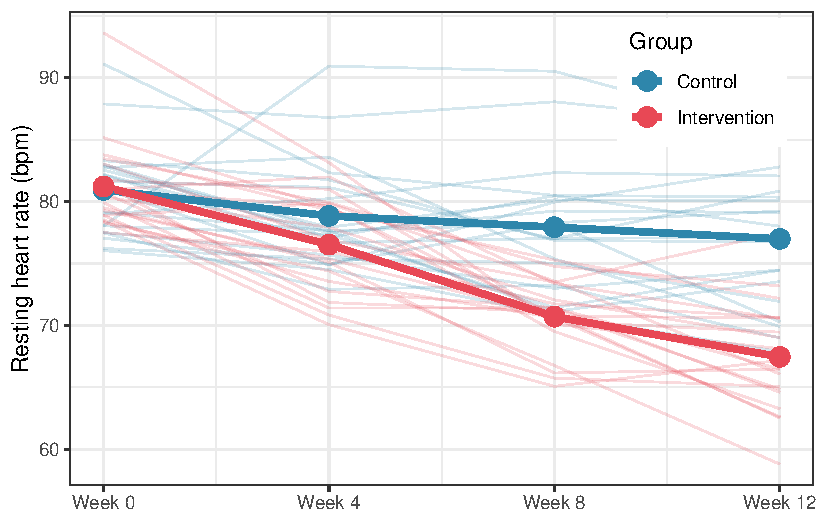
\includegraphics[width=0.9\textwidth,height=\textheight]{03d-repeated-measures_files/figure-pdf/fig-rm-plot-1.pdf}

}

\caption{\label{fig-rm-plot}Mean resting heart rate trajectories for
control and intervention groups across four time points. Thin lines show
individual patient trajectories; thick lines connect group means. The
intervention group shows a steeper and more sustained decline in heart
rate from week 4 onward, suggesting a group-by-time interaction. The
parallel trajectories at baseline confirm that the two groups were
comparable at the start of the trial.}

\end{figure}%

\subsection{Checking Sphericity}\label{checking-sphericity}

\begin{Shaded}
\begin{Highlighting}[]
\FunctionTok{library}\NormalTok{(car)}

\CommentTok{\# car::Anova requires wide format with group as a between{-}subjects predictor}
\NormalTok{fit\_mlm }\OtherTok{\textless{}{-}} \FunctionTok{lm}\NormalTok{(}\FunctionTok{cbind}\NormalTok{(t1, t2, t3, t4) }\SpecialCharTok{\textasciitilde{}}\NormalTok{ group, }\AttributeTok{data =}\NormalTok{ cardiac\_recovery\_wide)}
\NormalTok{idata }\OtherTok{\textless{}{-}} \FunctionTok{data.frame}\NormalTok{(}\AttributeTok{time =} \FunctionTok{factor}\NormalTok{(}\FunctionTok{c}\NormalTok{(}\StringTok{"t1"}\NormalTok{, }\StringTok{"t2"}\NormalTok{, }\StringTok{"t3"}\NormalTok{, }\StringTok{"t4"}\NormalTok{)))}

\NormalTok{rm\_model }\OtherTok{\textless{}{-}} \FunctionTok{Anova}\NormalTok{(fit\_mlm, }\AttributeTok{idata =}\NormalTok{ idata, }\AttributeTok{idesign =} \SpecialCharTok{\textasciitilde{}}\NormalTok{ time, }\AttributeTok{type =} \StringTok{"III"}\NormalTok{)}

\CommentTok{\# Full output: Mauchly\textquotesingle{}s test + epsilon corrections + F tests}
\FunctionTok{summary}\NormalTok{(rm\_model, }\AttributeTok{multivariate =} \ConstantTok{FALSE}\NormalTok{)}
\end{Highlighting}
\end{Shaded}

\begin{verbatim}
#> 
#> Univariate Type III Repeated-Measures ANOVA Assuming Sphericity
#> 
#>             Sum Sq num Df Error SS den Df    F value    Pr(>F)    
#> (Intercept) 495174      1   1757.9     38 10704.0589 < 2.2e-16 ***
#> group          883      1   1757.9     38    19.0945 9.292e-05 ***
#> time           172      3   1027.7    114     6.3681  0.000498 ***
#> group:time     599      3   1027.7    114    22.1398 2.280e-11 ***
#> ---
#> Signif. codes:  0 '***' 0.001 '**' 0.01 '*' 0.05 '.' 0.1 ' ' 1
#> 
#> 
#> Mauchly Tests for Sphericity
#> 
#>            Test statistic p-value
#> time              0.67608 0.01343
#> group:time        0.67608 0.01343
#> 
#> 
#> Greenhouse-Geisser and Huynh-Feldt Corrections
#>  for Departure from Sphericity
#> 
#>             GG eps Pr(>F[GG])    
#> time       0.80607   0.001348 ** 
#> group:time 0.80607  1.377e-09 ***
#> ---
#> Signif. codes:  0 '***' 0.001 '**' 0.01 '*' 0.05 '.' 0.1 ' ' 1
#> 
#>              HF eps   Pr(>F[HF])
#> time       0.864768 9.960634e-04
#> group:time 0.864768 3.972709e-10
\end{verbatim}

Mauchly's test is significant (\(W = 0.676\), \(p = 0.013\)), indicating
that the sphericity assumption is violated. The variances of the
pairwise differences between time points are not equal across all
combinations, which means the standard F test degrees of freedom are
inflated and uncorrected p-values cannot be trusted.

The Greenhouse-Geisser estimate is \(\hat{\varepsilon}_{GG} = 0.806\).
Since this exceeds the 0.75 threshold, the Huynh-Feldt correction is
preferred over the more conservative Greenhouse-Geisser. The Huynh-Feldt
estimate is \(\tilde{\varepsilon}_{HF} = 0.865\), reasonably close to 1,
indicating that the departure from sphericity is moderate rather than
severe. We therefore use the Huynh-Feldt corrected p-values for all
within-subject tests.

The corrected ANOVA table tells a clear story. The group-by-time
interaction is highly significant (\(F_{2.59, 98.6} = 22.14\),
\(p = 3.97 \times 10^{-10}\), using Huynh-Feldt corrected degrees of
freedom), confirming that the two rehabilitation programmes produce
different heart rate trajectories over the 12-week period. This is the
primary finding of the study. The main effect of time is also
significant (\(F_{2.59, 98.6} = 6.37\), \(p < 0.001\)), indicating that
heart rate declines over the course of rehabilitation when averaged
across both groups. The main effect of group is significant as well
(\(F_{1, 38} = 19.09\), \(p < 0.001\)), though as noted earlier this
averages over a trajectory that differs between groups and should not be
interpreted in isolation from the interaction.

Two things are worth noting for students reading this output for the
first time. First, the uncorrected p-values (assuming sphericity) and
the corrected p-values tell the same qualitative story here: all three
effects remain highly significant after correction. This is because the
violation is moderate (\(\tilde{\varepsilon}_{HF} = 0.865\)) rather than
severe. With a more serious violation, the correction can shift a
borderline result from significant to non-significant, which is
precisely why it must not be skipped. Second, the degrees of freedom in
the corrected tests are no longer whole numbers, they are
\(\hat{\varepsilon} \times df_{\text{uncorrected}}\). This is not a
typographical error; it is the mathematical consequence of the epsilon
adjustment and is entirely normal in repeated measures output.

\subsection{Fitting the Model and Interpreting
Results}\label{fitting-the-model-and-interpreting-results}

\begin{Shaded}
\begin{Highlighting}[]
\CommentTok{\# Base R aov() approach for the ANOVA table}
\NormalTok{fit\_rm }\OtherTok{\textless{}{-}} \FunctionTok{aov}\NormalTok{(hr }\SpecialCharTok{\textasciitilde{}}\NormalTok{ group }\SpecialCharTok{*}\NormalTok{ time }\SpecialCharTok{+} \FunctionTok{Error}\NormalTok{(subject}\SpecialCharTok{/}\NormalTok{time), }\AttributeTok{data =}\NormalTok{ cardiac\_recovery)}
\FunctionTok{summary}\NormalTok{(fit\_rm)}
\end{Highlighting}
\end{Shaded}

\begin{verbatim}
#> 
#> Error: subject
#>           Df Sum Sq Mean Sq F value   Pr(>F)    
#> group      1  883.3   883.3   19.09 9.29e-05 ***
#> Residuals 38 1757.9    46.3                     
#> ---
#> Signif. codes:  0 '***' 0.001 '**' 0.01 '*' 0.05 '.' 0.1 ' ' 1
#> 
#> Error: subject:time
#>             Df Sum Sq Mean Sq F value   Pr(>F)    
#> time         3 1811.6   603.9   66.98  < 2e-16 ***
#> group:time   3  598.8   199.6   22.14 2.28e-11 ***
#> Residuals  114 1027.7     9.0                     
#> ---
#> Signif. codes:  0 '***' 0.001 '**' 0.01 '*' 0.05 '.' 0.1 ' ' 1
\end{verbatim}

The output is split into two error strata, which is the defining
structural feature of repeated measures ANOVA output in R and the first
thing students need to learn to read correctly.

The \textbf{\texttt{Error:\ subject} stratum} captures the
between-subjects variation i.e.~differences among individuals that
persist across all time points. It contains the test for the
between-subjects factor \texttt{group}. The intervention group differs
significantly from the control group in its overall mean heart rate
(\(F_{1,38} = 19.09\), \(p < 0.001\)), but as discussed above, this
average difference collapsed across all four time points is not the
primary question. The residual mean square in this stratum (46.3 bpm²)
estimates the stable between-patient variance: the variation in baseline
heart rate that exists among individuals regardless of which programme
they followed.

The \textbf{\texttt{Error:\ subject:time} stratum} captures the
within-subjects variation i.e.~how each individual's heart rate changes
across time points. It contains the tests for the within-subjects factor
\texttt{time} and the \texttt{group:time} interaction. The residual mean
square here (9.0 bpm²) is dramatically smaller than the between-subjects
residual (46.3 bpm²), illustrating concretely the power advantage of
repeated measures designs: the stable individual differences that would
inflate the error term in a between-subjects design have been
partitioned out, leaving a much smaller noise floor against which the
within-subjects effects are tested.

The main effect of time is highly significant (\(F_{3,114} = 66.98\),
\(p < 0.001\)), confirming that heart rate declines substantially over
the 12-week rehabilitation period when averaged across both groups. This
is not surprising, indeed rehabilitation of any kind is expected to
improve cardiovascular fitness, but it is a necessary finding that
validates the study's measurement protocol.

Most importantly, the group-by-time interaction is highly significant
(\(F_{3,114} = 22.14\), \(p < 0.001\)). This is the central result: the
trajectory of heart rate change over 12 weeks differs between the two
rehabilitation programmes. The intensive programme produces a steeper
and more sustained decline in resting heart rate than the standard
programme, and this difference cannot be attributed to chance. Note that
these are the uncorrected degrees of freedom, since Mauchly's test was
significant, the Huynh-Feldt corrected p-values from
\texttt{car::Anova()} should be reported, which remain highly
significant (\(p = 3.97 \times 10^{-10}\)) and lead to the same
conclusion.

It is also worth noting the ratio of the two residual mean squares. The
between-subjects residual (46.3 bpm²) is more than five times larger
than the within-subjects residual (9.0 bpm²). This tells us that
individuals differ substantially from one another in their baseline
heart rate, but that within any given individual the
measurement-to-measurement variation is much smaller. This is exactly
the pattern that makes repeated measures designs efficient: by tracking
individuals over time rather than comparing independent groups, we are
testing the treatment effect against within-person variability rather
than between-person variability, gaining statistical sensitivity as a
direct consequence.

\subsection{Effect Sizes and
Reporting}\label{effect-sizes-and-reporting}

\begin{Shaded}
\begin{Highlighting}[]
\FunctionTok{library}\NormalTok{(effectsize)}

\FunctionTok{eta\_squared}\NormalTok{(fit\_rm, }\AttributeTok{partial =} \ConstantTok{TRUE}\NormalTok{)}
\end{Highlighting}
\end{Shaded}

\begin{verbatim}
#> # Effect Size for ANOVA (Type I)
#> 
#> Group        |  Parameter | Eta2 (partial) |       95% CI
#> ---------------------------------------------------------
#> subject      |      group |           0.33 | [0.14, 1.00]
#> subject:time |       time |           0.64 | [0.55, 1.00]
#> subject:time | group:time |           0.37 | [0.25, 1.00]
#> 
#> - One-sided CIs: upper bound fixed at [1.00].
\end{verbatim}

The partial \(\eta^2\) values reveal the relative importance of each
effect in the model. Time explains the largest share of within-subject
variance (partial \(\eta^2 = 0.64\), 95\% CI \([0.55, 1.00]\)),
indicating that 64\% of the within-subject variation in heart rate is
accounted for by the progression across the 12 weeks which is a large
effect by any standard, reflecting the genuine and consistent
improvement in cardiovascular fitness that rehabilitation produces
regardless of programme type.

The group-by-time interaction has a partial \(\eta^2 = 0.37\) (95\% CI
\([0.25, 1.00]\)), a large effect indicating that 37\% of the
within-subject variance not explained by time alone is attributable to
the differential trajectory of the two groups. This is the
scientifically meaningful result: not only does heart rate improve over
time, but it improves substantially more, and more rapidly, in the
intensive rehabilitation group than in the control group.

The between-subjects effect of group has a partial \(\eta^2 = 0.33\)
(95\% CI \([0.14, 1.00]\)), indicating that 33\% of the stable
between-patient variance is explained by group membership. This reflects
the sustained overall difference in heart rate between the two groups
when averaged across all time points.

A note on the confidence intervals: all upper bounds are fixed at 1.00,
which is expected for one-sided confidence intervals on \(\eta^2\) as
the parameter is bounded above by 1 by definition. The lower bounds are
the more informative values, confirming that even at the conservative
end of the interval, all three effects are meaningfully large.

The complete report of this analysis reads:

\begin{quote}
A two-way mixed repeated measures ANOVA examined the effect of
rehabilitation programme (between-subjects: control vs intervention,
\(n = 20\) per group) and time (within-subjects: weeks 0, 4, 8, 12) on
resting heart rate. Mauchly's test indicated a significant violation of
sphericity (\(W = 0.676\), \(p = 0.013\)); Huynh-Feldt corrected degrees
of freedom were therefore applied to all within-subjects tests
(\(\tilde{\varepsilon}_{HF} = 0.865\)). A highly significant
group-by-time interaction was found (\(F_{2.59, 98.6} = 22.14\),
\(p = 3.97 \times 10^{-10}\), partial \(\eta^2 = 0.37\)), indicating
that the intensive rehabilitation programme produced a steeper decline
in resting heart rate over the 12-week period than the standard
programme. A significant main effect of time confirmed that heart rate
declined across the study period in both groups
(\(F_{2.59, 98.6} = 6.37\), \(p < 0.001\), partial \(\eta^2 = 0.64\)).
The main effect of group was also significant (\(F_{1, 38} = 19.09\),
\(p < 0.001\), partial \(\eta^2 = 0.33\)), reflecting the overall lower
mean heart rate in the intervention group across all time points. These
results support the conclusion that intensive cardiac rehabilitation
produces clinically meaningful improvements in resting heart rate beyond
those achieved by standard care alone.
\end{quote}

\subsection{A Note on Missing Data}\label{a-note-on-missing-data}

Repeated measures ANOVA as implemented in \texttt{aov()} and
\texttt{car::Anova()} requires complete data: every subject must have a
measurement at every time point. If any observations are missing, the
subject is excluded entirely from the analysis. In a 12-week clinical
trial, dropout is almost inevitable: patients move, recover, or withdraw
consent.

When missing data are present, the appropriate tool is a \textbf{linear
mixed-effects model} (Chapter 9), which can handle incomplete
longitudinal data under the assumption that missingness is random (the
missing-at-random assumption). The mixed model fitted to complete data
will give identical results to repeated measures ANOVA in the balanced
case, confirming that repeated measures ANOVA is simply a special case
of the linear mixed model, a theme that runs throughout Part III of this
book.

\chapter{Split-Plot and Nested Designs}\label{sec-chap7}

Every ANOVA design considered so far has shared a common simplifying
assumption: that the experimental units receiving different treatments
are all of the same type, at the same level of organisation, and subject
to the same sources of variation. A plant is a plant, a patient is a
patient, a plot is a plot.

Biological reality is rarely so flat. Ecosystems are organised in
layers: individual organisms live within plots, plots within fields,
fields within regions. Clinical trials recruit patients from hospitals,
hospitals from healthcare systems. Agricultural experiments apply
whole-farm treatments to fields and within-field treatments to plots. In
all of these cases, the experimental units exist at multiple levels of a
hierarchy, and treatments are applied, and therefore replicated, at
different levels of that hierarchy.

Ignoring this hierarchical structure leads directly to the
pseudoreplication problem introduced in Chapter 2. Accounting for it
correctly requires designs and analyses that explicitly represent the
nested structure of the data. This chapter introduces the two most
important such designs in biological research: the split-plot and the
nested ANOVA.

\section{Hierarchy in Biological Data: Why It Cannot Be
Ignored}\label{hierarchy-in-biological-data-why-it-cannot-be-ignored}

\subsection{Everything Is Nested in
Something}\label{everything-is-nested-in-something}

Before introducing any new design, it is worth pausing to build a clear
intuition for what hierarchical structure means and why it demands
special treatment.

Consider a simple example. A researcher wants to study the effect of two
soil treatments (amended vs unamended) and two plant varieties (A vs B)
on crop yield. She has access to four large fields. Two fields receive
the soil amendment; two do not. Within each field, she establishes four
plots: two planted with Variety A and two with Variety B. She measures
yield from five plants within each plot.

The data have three levels of organisation:

\[\text{Field} \supset \text{Plot} \supset \text{Plant}\]

This is a hierarchy. Fields are nested within soil treatment. Plots are
nested within fields. Plants are nested within plots. Each level has its
own sources of variation: fields differ from each other in ways that
have nothing to do with soil treatment (drainage, history,
microclimate); plots within a field differ from each other in ways that
have nothing to do with variety (position, local soil variation); plants
within a plot differ from each other due to individual biological
variation.

The critical point is that \textbf{the treatment is applied and
replicated at the field level, not the plot level and not the plant
level.} The soil amendment was not randomly assigned to individual
plants: \emph{it was assigned to whole fields}. The field is therefore
the unit of replication for the soil treatment comparison, and there are
only two replicates per treatment (\(n = 2\) fields per treatment), not
\(2 \times 4 \times 5 = 40\).

\subsection{What Goes Wrong When You Ignore the
Hierarchy}\label{what-goes-wrong-when-you-ignore-the-hierarchy}

If the researcher analyses this experiment by running a standard ANOVA
on all \(4 \times 4 \times 5 = 80\) plant measurements, treating each
plant as an independent observation, she is pseudoreplicating at two
levels simultaneously. The within-field and within-plot correlation
structures are ignored, and the error term used to test the soil
treatment effect is the plant-level residual, which is far too small,
because it does not account for the field-to-field variation that is the
appropriate noise against which the treatment should be judged.

The simulation below demonstrates the inflation of the false positive
rate that results:

\begin{Shaded}
\begin{Highlighting}[]
\FunctionTok{library}\NormalTok{(future)}
\FunctionTok{library}\NormalTok{(furrr)}
\FunctionTok{library}\NormalTok{(purrr)}

\FunctionTok{plan}\NormalTok{(multisession)}

\FunctionTok{set.seed}\NormalTok{(}\DecValTok{42}\NormalTok{)}
\NormalTok{n\_sim }\OtherTok{\textless{}{-}} \DecValTok{5000}
\NormalTok{alpha }\OtherTok{\textless{}{-}} \FloatTok{0.05}
\NormalTok{n\_fields }\OtherTok{\textless{}{-}} \DecValTok{4}      \CommentTok{\# 2 per treatment}
\NormalTok{n\_plots }\OtherTok{\textless{}{-}} \DecValTok{4}      \CommentTok{\# per field}
\NormalTok{n\_plants }\OtherTok{\textless{}{-}} \DecValTok{5}      \CommentTok{\# per plot}
\NormalTok{field\_sd }\OtherTok{\textless{}{-}} \DecValTok{3}      \CommentTok{\# field{-}to{-}field variation}
\NormalTok{plot\_sd }\OtherTok{\textless{}{-}} \DecValTok{2}      \CommentTok{\# plot{-}to{-}plot variation within field}
\NormalTok{plant\_sd }\OtherTok{\textless{}{-}} \DecValTok{1}      \CommentTok{\# plant{-}to{-}plant variation within plot}

\NormalTok{results }\OtherTok{\textless{}{-}} \FunctionTok{future\_map\_dfr}\NormalTok{(}\FunctionTok{seq\_len}\NormalTok{(n\_sim), }\ControlFlowTok{function}\NormalTok{(i) \{}
  
\NormalTok{  treatment   }\OtherTok{\textless{}{-}} \FunctionTok{rep}\NormalTok{(}\FunctionTok{c}\NormalTok{(}\StringTok{"Control"}\NormalTok{, }\StringTok{"Amended"}\NormalTok{), }\AttributeTok{each =}\NormalTok{ n\_fields }\SpecialCharTok{/} \DecValTok{2}\NormalTok{)}
\NormalTok{  field\_effect }\OtherTok{\textless{}{-}} \FunctionTok{rnorm}\NormalTok{(n\_fields, }\DecValTok{0}\NormalTok{, field\_sd)}
  
\NormalTok{  df }\OtherTok{\textless{}{-}} \FunctionTok{do.call}\NormalTok{(rbind, }\FunctionTok{lapply}\NormalTok{(}\FunctionTok{seq\_len}\NormalTok{(n\_fields), }\ControlFlowTok{function}\NormalTok{(f) \{}
    \FunctionTok{do.call}\NormalTok{(rbind, }\FunctionTok{lapply}\NormalTok{(}\FunctionTok{seq\_len}\NormalTok{(n\_plots), }\ControlFlowTok{function}\NormalTok{(p) \{}
\NormalTok{      plot\_effect }\OtherTok{\textless{}{-}} \FunctionTok{rnorm}\NormalTok{(}\DecValTok{1}\NormalTok{, }\DecValTok{0}\NormalTok{, plot\_sd)}
      \FunctionTok{data.frame}\NormalTok{(}
        \AttributeTok{yield =} \FunctionTok{rnorm}\NormalTok{(n\_plants, }\AttributeTok{mean =} \DecValTok{50} \SpecialCharTok{+}\NormalTok{ field\_effect[f] }\SpecialCharTok{+}\NormalTok{ plot\_effect, }\AttributeTok{sd =}\NormalTok{ plant\_sd),}
        \AttributeTok{treatment =}\NormalTok{ treatment[f],}
        \AttributeTok{field =} \FunctionTok{factor}\NormalTok{(f),}
        \AttributeTok{plot =} \FunctionTok{factor}\NormalTok{(}\FunctionTok{paste}\NormalTok{(f, p, }\AttributeTok{sep =} \StringTok{"\_"}\NormalTok{))}
\NormalTok{      )}
\NormalTok{    \}))}
\NormalTok{  \}))}
  
  \CommentTok{\# Wrong: treat all plants as independent}
\NormalTok{  p\_wrong }\OtherTok{\textless{}{-}} \FunctionTok{summary}\NormalTok{(}
    \FunctionTok{aov}\NormalTok{(yield }\SpecialCharTok{\textasciitilde{}}\NormalTok{ treatment, }\AttributeTok{data =}\NormalTok{ df)}
\NormalTok{  )[[}\DecValTok{1}\NormalTok{]][[}\StringTok{"Pr(\textgreater{}F)"}\NormalTok{]][}\DecValTok{1}\NormalTok{]}
  
  \CommentTok{\# Correct: use field means as the unit of analysis}
\NormalTok{  field\_means }\OtherTok{\textless{}{-}} \FunctionTok{aggregate}\NormalTok{(yield }\SpecialCharTok{\textasciitilde{}}\NormalTok{ treatment }\SpecialCharTok{+}\NormalTok{ field,}
                           \AttributeTok{data =}\NormalTok{ df, }\AttributeTok{FUN =}\NormalTok{ mean)}
\NormalTok{  p\_correct }\OtherTok{\textless{}{-}} \FunctionTok{summary}\NormalTok{(}
    \FunctionTok{aov}\NormalTok{(yield }\SpecialCharTok{\textasciitilde{}}\NormalTok{ treatment, }\AttributeTok{data =}\NormalTok{ field\_means)}
\NormalTok{  )[[}\DecValTok{1}\NormalTok{]][[}\StringTok{"Pr(\textgreater{}F)"}\NormalTok{]][}\DecValTok{1}\NormalTok{]}
  
  \FunctionTok{data.frame}\NormalTok{(}\AttributeTok{p\_wrong =}\NormalTok{ p\_wrong, }\AttributeTok{p\_correct =}\NormalTok{ p\_correct)}
  
\NormalTok{\}, }\AttributeTok{.options =} \FunctionTok{furrr\_options}\NormalTok{(}\AttributeTok{seed =} \ConstantTok{TRUE}\NormalTok{))}

\FunctionTok{plan}\NormalTok{(sequential)}
\end{Highlighting}
\end{Shaded}

\begin{Shaded}
\begin{Highlighting}[]
\CommentTok{\# View the simulated data}
\FunctionTok{head}\NormalTok{(results, }\AttributeTok{n =} \DecValTok{10}\NormalTok{)}
\end{Highlighting}
\end{Shaded}

\begin{verbatim}
#>         p_wrong p_correct
#> 1  1.713975e-02 0.4803663
#> 2  1.914645e-05 0.3266718
#> 3  9.265631e-01 0.9875177
#> 4  7.418683e-09 0.2185384
#> 5  7.697033e-05 0.4926903
#> 6  8.143981e-01 0.9355019
#> 7  2.013291e-01 0.8170871
#> 8  1.935473e-01 0.8389504
#> 9  4.284297e-20 0.1088934
#> 10 4.178010e-01 0.8922692
\end{verbatim}

\begin{Shaded}
\begin{Highlighting}[]
\FunctionTok{cat}\NormalTok{(}
  \StringTok{"False positive rate ignoring hierarchy:"}\NormalTok{,}
  \FunctionTok{round}\NormalTok{(}\FunctionTok{mean}\NormalTok{(results}\SpecialCharTok{$}\NormalTok{p\_wrong   }\SpecialCharTok{\textless{}}\NormalTok{ alpha), }\DecValTok{3}\NormalTok{),}
  \StringTok{"}\SpecialCharTok{\textbackslash{}n}\StringTok{False positive rate correct analysis:"}\NormalTok{,}
  \FunctionTok{round}\NormalTok{(}\FunctionTok{mean}\NormalTok{(results}\SpecialCharTok{$}\NormalTok{p\_correct }\SpecialCharTok{\textless{}}\NormalTok{ alpha), }\DecValTok{3}\NormalTok{), }\StringTok{"}\SpecialCharTok{\textbackslash{}n}\StringTok{"}
\NormalTok{  )}
\end{Highlighting}
\end{Shaded}

\begin{verbatim}
#> False positive rate ignoring hierarchy: 0.681 
#> False positive rate correct analysis: 0.05
\end{verbatim}

The false positive rate from the naive analysis is far above 5\%
(0.681), while the correct analysis, using field means as the unit of
analysis for the field-level treatment, stays at the nominal level. This
is the pseudoreplication problem from Chapter 2, now seen in a
hierarchical context.

\subsection{Visualising the Hierarchy}\label{visualising-the-hierarchy}

It helps to draw the structure of a hierarchical experiment explicitly
before deciding how to analyse it. For the field-plot-plant example:

\begin{figure}

\centering{


\includegraphics[width=5.71in,height=6.05in]{03e-split-plot-nested_files/figure-latex/mermaid-figure-1.png}

}

\caption{\label{fig-hierarchy-diagram}Hierarchical structure of the
field experiment. Soil treatment is applied at the field level and
replicated across fields. Variety is applied at the plot level within
each field. Plants are the observational unit at the bottom of the
hierarchy.}

\end{figure}%

\subsection{The Golden Rule of Hierarchical
Analysis}\label{the-golden-rule-of-hierarchical-analysis}

The rule that prevents most hierarchical analysis errors can be stated
simply:

\begin{quote}
\textbf{The error term used to test a treatment effect must come from
the same level of the hierarchy at which that treatment was applied and
randomised.}
\end{quote}

If soil amendment was randomised across fields, the field-to-field
variation is the correct error term for testing the amendment effect. If
variety was randomised across plots within fields, the plot-to-plot
variation within fields is the correct error term for testing the
variety effect. Using plant-level variation to test a field-level
treatment is like using a ruler calibrated in millimetres to measure a
distance that varies in kilometres, the instrument is simply measuring
the wrong thing.

This rule is the conceptual foundation of both split-plot and nested
ANOVA designs, which formalise it into a statistical framework.

\section{Pseudoreplication: The Silent Epidemic in
Biology}\label{sec-pseudoreplication2}

\subsection{A Pervasive Problem}\label{a-pervasive-problem}

In their landmark 1984 paper, Hurlbert \citeyearpar{hurlbert1984}
documented that pseudoreplication, the treatment of non-independent
observations as independent replicates, was present in a substantial
fraction of published ecological field experiments. Subsequent reviews
have found similar rates across ecology, agriculture, and biomedical
research. The problem has not gone away.

Pseudoreplication takes several distinct forms in practice, and being
able to recognise each is an essential skill.

\textbf{Simple pseudoreplication} occurs when multiple measurements are
taken from a single experimental unit and treated as independent
replicates. Six measurements of soil nitrogen from the same plot do not
give you six independent replicates, they give you six estimates of the
nitrogen level in one plot. The plot is still \(n = 1\).

\textbf{Sacrificial pseudoreplication} occurs when the analysis is
conducted at the wrong level of the hierarchy, as in the field example
above. The name reflects the fact that the correct, but lower-powered,
analysis is sacrificed in favour of an inflated, incorrect one.

\textbf{Temporal pseudoreplication} occurs when the same unit is
measured repeatedly over time and the measurements are treated as
independent. This is the repeated measures problem from Chapter 6 seen
in a field ecology context: a plot measured in spring, summer, and
autumn provides three measurements of the same plot, not three
independent plots.

\subsection{How to Avoid It}\label{how-to-avoid-it}

The antidote to pseudoreplication is to identify the experimental unit,
the smallest unit that was independently assigned to a treatment, before
the analysis begins, and to ensure that the unit of analysis matches the
unit of replication. When subsampling within units is necessary (for
precision, or because the response must be measured at a finer scale
than the treatment was applied), the subsamples should be averaged to
the level of the experimental unit before analysis, or the hierarchical
structure should be modelled explicitly.

\section{Split-Plot Design: Structure and Correct Error
Terms}\label{split-plot-design-structure-and-correct-error-terms}

\subsection{When Does a Split-Plot Design
Arise?}\label{when-does-a-split-plot-design-arise}

A split-plot design arises naturally when two factors must be tested but
one is much more difficult or expensive to change than the other. The
classic agricultural example: irrigation regime (irrigated vs rainfed)
must be applied to whole large fields because irrigation infrastructure
cannot be changed plot by plot, while fertiliser type can be applied to
much smaller individual plots within each field.

The experiment therefore applies the hard-to-change factor
(\textbf{whole-plot factor}) to large units (\textbf{whole plots}), then
subdivides each whole plot into smaller units (\textbf{sub-plots}) and
applies the easy-to-change factor (\textbf{sub-plot factor}) to those.

This structure is not merely a practical compromise, it is a deliberate
design choice that must be reflected in the analysis. The two factors
are tested against different error terms, because they were randomised
at different levels of the hierarchy.

\subsection{Structure of the Split-Plot
Design}\label{structure-of-the-split-plot-design}

With \(a\) levels of the whole-plot factor \(A\), \(b\) levels of the
sub-plot factor \(B\), and \(r\) whole-plot replicates per level of
\(A\):

\begin{itemize}
\tightlist
\item
  There are \(a \times r\) whole plots in total.
\item
  Each whole plot is divided into \(b\) sub-plots.
\item
  Total observations: \(a \times r \times b\).
\end{itemize}

The two error terms are:

\begin{itemize}
\tightlist
\item
  \textbf{Whole-plot error (\(MS_{WP}\)):} the variation among whole
  plots within the same level of \(A\). This is the correct error term
  for testing the main effect of \(A\).
\item
  \textbf{Sub-plot error (\(MS_{SP}\)):} the variation among sub-plots
  within the same whole plot. This is the correct error term for testing
  the main effect of \(B\) and the \(A \times B\) interaction.
\end{itemize}

The sub-plot error is typically smaller than the whole-plot error, which
is why the sub-plot factor and the interaction are tested with more
power than the whole-plot factor, a direct consequence of the design
structure.

\subsection{The Split-Plot Model}\label{the-split-plot-model}

\[y_{ijk} = \mu + \alpha_i + \delta_{ij} + \beta_k +
            (\alpha\beta)_{ik} + \varepsilon_{ijk}\]

where \(\alpha_i\) is the whole-plot treatment effect, \(\delta_{ij}\)
is the whole-plot error (variation among whole plots within treatment
\(i\), the error term for \(A\)), \(\beta_k\) is the sub-plot treatment
effect, \((\alpha\beta)_{ik}\) is the interaction, and
\(\varepsilon_{ijk}\) is the sub-plot error (the error term for \(B\)
and \(A \times B\)).

In R, the two error terms are specified explicitly using the
\texttt{Error()} term in \texttt{aov()}:

\begin{Shaded}
\begin{Highlighting}[]
\CommentTok{\# whole.plot: the unit receiving the whole{-}plot treatment}
\CommentTok{\# A: whole{-}plot factor}
\CommentTok{\# B: sub{-}plot factor}

\NormalTok{fit\_sp }\OtherTok{\textless{}{-}} \FunctionTok{aov}\NormalTok{(y }\SpecialCharTok{\textasciitilde{}}\NormalTok{ A }\SpecialCharTok{*}\NormalTok{ B }\SpecialCharTok{+} \FunctionTok{Error}\NormalTok{(whole.plot}\SpecialCharTok{/}\NormalTok{B), }\AttributeTok{data =}\NormalTok{ df)}
\FunctionTok{summary}\NormalTok{(fit\_sp)}
\end{Highlighting}
\end{Shaded}

\section{Nested ANOVA: Subsampling vs True
Replication}\label{nested-anova-subsampling-vs-true-replication}

\subsection{The Nested Structure}\label{the-nested-structure}

A nested design arises when the levels of one factor exist entirely
within the levels of another, and the levels of the inner factor are not
the same across levels of the outer factor. Fields contain plots, but
the plots in Field 1 are different from the plots in Field 2 as they are
nested within their respective fields, not crossed with them.

This is distinct from a factorial design, where every level of every
factor is combined with every level of every other factor. In a
factorial design, Variety A appears in both the irrigated and rainfed
fields. In a nested design, the plots in Field 1 are unique to Field 1.

The nested ANOVA model for two levels of nesting:

\[y_{ijk} = \mu + \alpha_i + \beta_{j(i)} + \varepsilon_{ijk}\]

where \(\alpha_i\) is the effect of the outer factor \(A\) at level
\(i\), \(\beta_{j(i)}\) is the effect of the inner factor \(B\) at level
\(j\) nested within level \(i\) of \(A\) (denoted \(j(i)\)), and
\(\varepsilon_{ijk}\) is the residual.

In R:

\begin{Shaded}
\begin{Highlighting}[]
\CommentTok{\# B is nested within A}
\NormalTok{fit\_nested }\OtherTok{\textless{}{-}} \FunctionTok{aov}\NormalTok{(y }\SpecialCharTok{\textasciitilde{}}\NormalTok{ A }\SpecialCharTok{+}\NormalTok{ B }\SpecialCharTok{\%in\%}\NormalTok{ A, }\AttributeTok{data =}\NormalTok{ df)}
\CommentTok{\# Equivalently:}
\NormalTok{fit\_nested }\OtherTok{\textless{}{-}} \FunctionTok{aov}\NormalTok{(y }\SpecialCharTok{\textasciitilde{}}\NormalTok{ A}\SpecialCharTok{/}\NormalTok{B, }\AttributeTok{data =}\NormalTok{ df)}
\FunctionTok{summary}\NormalTok{(fit\_nested)}
\end{Highlighting}
\end{Shaded}

\subsection{Subsampling vs True
Replication}\label{subsampling-vs-true-replication}

The most important practical distinction in nested designs is between
\textbf{true replication} and \textbf{subsampling}. True replicates are
independent experimental units that each received a treatment
independently. Subsamples are multiple measurements taken from the same
experimental unit.

\begin{longtable}[]{@{}
  >{\raggedright\arraybackslash}p{(\columnwidth - 4\tabcolsep) * \real{0.2500}}
  >{\raggedright\arraybackslash}p{(\columnwidth - 4\tabcolsep) * \real{0.3750}}
  >{\raggedright\arraybackslash}p{(\columnwidth - 4\tabcolsep) * \real{0.3750}}@{}}
\toprule\noalign{}
\begin{minipage}[b]{\linewidth}\raggedright
\end{minipage} & \begin{minipage}[b]{\linewidth}\raggedright
True replicates
\end{minipage} & \begin{minipage}[b]{\linewidth}\raggedright
Subsamples
\end{minipage} \\
\midrule\noalign{}
\endhead
\bottomrule\noalign{}
\endlastfoot
Definition & Independently treated units & Multiple measures of one
unit \\
Example & Four separately irrigated fields & Five soil cores from one
field \\
Contribution to \(n\) & Each counts as one replicate & Together count as
one replicate \\
Error term & Between-unit residual & Within-unit residual \\
\end{longtable}

Treating subsamples as true replicates is the most common form of
sacrificial pseudoreplication. The nested ANOVA correctly partitions the
variation into between-unit and within-unit components and uses the
appropriate error term for each.

\section{Example 1: Grazing Effects on Plant
Diversity}\label{example-1-grazing-effects-on-plant-diversity}

\subsection{The Study}\label{the-study-2}

An ecologist is investigating the effect of grazing intensity (ungrazed,
light grazing, heavy grazing) on plant species richness in a grassland
(Section~\ref{sec-grazing}). Six large paddocks are available, two
assigned to each grazing treatment. Within each paddock, four quadrats
are established and plant species richness is counted in each. Three
random soil cores are taken from each quadrat for soil nutrient
analysis, but species richness is the response of interest.

The structure is:

\[\text{Grazing treatment} \supset \text{Paddock} \supset \text{Quadrat}\]

Grazing treatment is the fixed factor of interest. Paddock is nested
within grazing treatment and is the unit of replication for the
treatment comparison. Quadrat is nested within paddock and provides
subsamples within the true replicates.

\begin{Shaded}
\begin{Highlighting}[]
\CommentTok{\# Show the simulated data}
\FunctionTok{summary}\NormalTok{(grazing)}
\end{Highlighting}
\end{Shaded}

\begin{verbatim}
#>     richness         treatment paddock
#>  Min.   : 3.000   Ungrazed:8   U1:4   
#>  1st Qu.: 6.750   Light   :8   U2:4   
#>  Median :10.500   Heavy   :8   L1:4   
#>  Mean   : 9.792                L2:4   
#>  3rd Qu.:13.250                H1:4   
#>  Max.   :15.000                H2:4
\end{verbatim}

\subsection{Correct Analysis: Paddock as the Error
Term}\label{correct-analysis-paddock-as-the-error-term}

\begin{Shaded}
\begin{Highlighting}[]
\CommentTok{\# Nested ANOVA: paddock nested within treatment}
\NormalTok{fit\_eco }\OtherTok{\textless{}{-}} \FunctionTok{aov}\NormalTok{(richness }\SpecialCharTok{\textasciitilde{}}\NormalTok{ treatment }\SpecialCharTok{+} \FunctionTok{Error}\NormalTok{(paddock}\SpecialCharTok{/}\NormalTok{treatment), }\AttributeTok{data =}\NormalTok{ grazing)}
\FunctionTok{summary}\NormalTok{(fit\_eco)}
\end{Highlighting}
\end{Shaded}

\begin{verbatim}
#> 
#> Error: paddock
#>           Df Sum Sq Mean Sq F value Pr(>F)  
#> treatment  2 303.58  151.79   23.81 0.0144 *
#> Residuals  3  19.13    6.38                 
#> ---
#> Signif. codes:  0 '***' 0.001 '**' 0.01 '*' 0.05 '.' 0.1 ' ' 1
#> 
#> Error: Within
#>           Df Sum Sq Mean Sq F value Pr(>F)
#> Residuals 18  35.25   1.958
\end{verbatim}

The output is split into two strata, each telling a different part of
the story.

The \textbf{\texttt{Error:\ paddock} stratum} is where the treatment
test lives. Grazing treatment has a significant effect on plant species
richness (\(F_{2,3} = 23.81\), \(p = 0.014\)). The residual mean square
in this stratum (6.38) estimates the paddock-to-paddock variation within
treatments i.e.~the genuine noise against which the treatment effect is
judged, since paddocks are the units that were independently assigned to
grazing treatments. This is the correct error term.

The \textbf{\texttt{Error:\ Within} stratum} captures the
quadrat-to-quadrat variation within paddocks, with a residual mean
square of 1.96. Notice that this is substantially smaller than the
paddock-level residual (6.38) meaning paddocks differ from each other
more than quadrats within the same paddock differ from each other. This
is the typical pattern in nested designs, and it is precisely why using
quadrat-level variation to test the treatment effect would be wrong: the
within-paddock noise floor is too low, and testing against it would make
the treatment appear far more significant than the actual replication
warrants.

With only two paddocks per treatment, the degrees of freedom for the
treatment test are low (\(df_{\text{treatment}} = 2\),
\(df_{\text{error}} = 3\)). This correctly reflects the limited
replication at the treatment level. No matter how many quadrats are
sampled within each paddock, the experiment has only six independent
units at the treatment level, and the analysis honestly acknowledges
this. The significant result (\(p = 0.014\)) is therefore a genuine
finding achieved with sparse replication, not an artefact of inflated
degrees of freedom.

\begin{Shaded}
\begin{Highlighting}[]
\CommentTok{\# Visualise}
\FunctionTok{library}\NormalTok{(ggplot2)}

\NormalTok{paddock\_means }\OtherTok{\textless{}{-}} \FunctionTok{aggregate}\NormalTok{(richness }\SpecialCharTok{\textasciitilde{}}\NormalTok{ treatment }\SpecialCharTok{+}\NormalTok{ paddock, }\AttributeTok{data =}\NormalTok{ grazing, }\AttributeTok{FUN =}\NormalTok{ mean)}

\FunctionTok{ggplot}\NormalTok{(grazing, }\FunctionTok{aes}\NormalTok{(}\AttributeTok{x =}\NormalTok{ treatment, }\AttributeTok{y =}\NormalTok{ richness, }\AttributeTok{colour =}\NormalTok{ treatment)) }\SpecialCharTok{+}
  \FunctionTok{geom\_jitter}\NormalTok{(}\AttributeTok{width =} \FloatTok{0.15}\NormalTok{, }\AttributeTok{alpha =} \FloatTok{0.4}\NormalTok{, }\AttributeTok{size =} \DecValTok{2}\NormalTok{) }\SpecialCharTok{+}
  \FunctionTok{geom\_point}\NormalTok{(}\AttributeTok{data =}\NormalTok{ paddock\_means, }\FunctionTok{aes}\NormalTok{(}\AttributeTok{y =}\NormalTok{ richness, }\AttributeTok{group =}\NormalTok{ paddock), }\AttributeTok{size =} \DecValTok{4}\NormalTok{, }\AttributeTok{shape =} \DecValTok{18}\NormalTok{) }\SpecialCharTok{+}
  \FunctionTok{stat\_summary}\NormalTok{(}\AttributeTok{fun =}\NormalTok{ mean, }\AttributeTok{geom =} \StringTok{"crossbar"}\NormalTok{, }\AttributeTok{width =} \FloatTok{0.4}\NormalTok{, }\AttributeTok{colour =} \StringTok{"grey30"}\NormalTok{, }\AttributeTok{linewidth =} \FloatTok{0.8}\NormalTok{) }\SpecialCharTok{+}
  \FunctionTok{scale\_colour\_manual}\NormalTok{(}\AttributeTok{values =} \FunctionTok{c}\NormalTok{(}\StringTok{"\#2E86AB"}\NormalTok{, }\StringTok{"\#F6AE2D"}\NormalTok{, }\StringTok{"\#E84855"}\NormalTok{)) }\SpecialCharTok{+}
  \FunctionTok{labs}\NormalTok{(}\AttributeTok{x =} \StringTok{"Grazing treatment"}\NormalTok{, }\AttributeTok{y =} \StringTok{"Species richness"}\NormalTok{, }\AttributeTok{colour =} \ConstantTok{NULL}\NormalTok{) }\SpecialCharTok{+}
  \FunctionTok{theme\_bw}\NormalTok{() }\SpecialCharTok{+}
  \FunctionTok{theme}\NormalTok{(}\AttributeTok{legend.position =} \StringTok{"none"}\NormalTok{)}
\end{Highlighting}
\end{Shaded}

\begin{center}
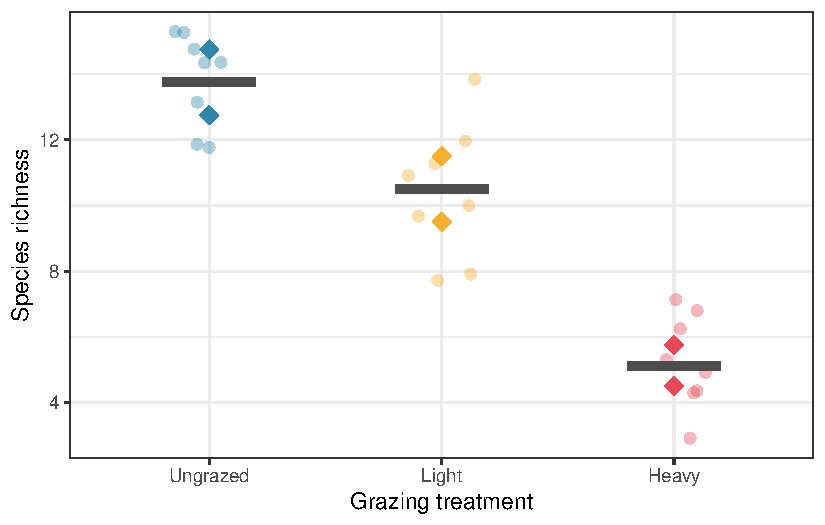
\includegraphics[width=0.9\textwidth,height=\textheight]{03e-split-plot-nested_files/figure-pdf/unnamed-chunk-4-1.pdf}
\end{center}

The analysis uses paddock as the correct error term for testing the
grazing treatment effect. With only two paddocks per treatment, the
degrees of freedom for the treatment test are low (\(df = 2\) for the
treatment, \(df = 3\) for the whole-plot error), correctly reflecting
the fact that the experiment has limited replication at the treatment
level, regardless of how many quadrats were sampled within each paddock.

\subsection{What Happens if You Ignore the
Nesting}\label{what-happens-if-you-ignore-the-nesting}

\begin{Shaded}
\begin{Highlighting}[]
\CommentTok{\# Wrong: treat all quadrats as independent}
\NormalTok{fit\_eco\_wrong }\OtherTok{\textless{}{-}} \FunctionTok{aov}\NormalTok{(richness }\SpecialCharTok{\textasciitilde{}}\NormalTok{ treatment, }\AttributeTok{data =}\NormalTok{ grazing)}
\FunctionTok{summary}\NormalTok{(fit\_eco\_wrong)}
\end{Highlighting}
\end{Shaded}

\begin{verbatim}
#>             Df Sum Sq Mean Sq F value   Pr(>F)    
#> treatment    2 303.58  151.79   58.62 2.55e-09 ***
#> Residuals   21  54.38    2.59                     
#> ---
#> Signif. codes:  0 '***' 0.001 '**' 0.01 '*' 0.05 '.' 0.1 ' ' 1
\end{verbatim}

\begin{Shaded}
\begin{Highlighting}[]
\FunctionTok{cat}\NormalTok{(}
  \StringTok{"}\SpecialCharTok{\textbackslash{}n}\StringTok{Correct df for treatment: 2, error df: 3}\SpecialCharTok{\textbackslash{}n}\StringTok{Wrong df for treatment: 2, error df:"}\NormalTok{,}
  \FunctionTok{df.residual}\NormalTok{(fit\_eco\_wrong), }\StringTok{"}\SpecialCharTok{\textbackslash{}n}\StringTok{"}
\NormalTok{  )}
\end{Highlighting}
\end{Shaded}

\begin{verbatim}
#> 
#> Correct df for treatment: 2, error df: 3
#> Wrong df for treatment: 2, error df: 21
\end{verbatim}

The naive analysis has \(df_{\text{error}} = 21\) instead of 3,
artificially inflating the power of the test by treating quadrat-level
variation as if it were independent replication of the treatment.

\section{Example 2: Irrigation and Fertiliser in a Split-Plot
Design}\label{example-2-irrigation-and-fertiliser-in-a-split-plot-design}

\subsection{The Study}\label{the-study-3}

An agronomist is testing two irrigation regimes (rainfed vs irrigated)
and three fertiliser types (none, nitrogen, phosphorus) on wheat yield
(Section~\ref{sec-irrig}). Irrigation is applied to whole fields (it
cannot be changed within a field) while fertiliser can be applied to
individual plots within each field. Six fields are available, three
assigned to each irrigation treatment. Each field is divided into three
plots, one for each fertiliser type.

This is a split-plot design:

\begin{itemize}
\tightlist
\item
  \textbf{Whole-plot factor:} irrigation (2 levels), replicated across 6
  fields (3 per treatment).
\item
  \textbf{Sub-plot factor:} fertiliser (3 levels), applied to plots
  within each field.
\item
  \textbf{Total observations:} \(6 \times 3 = 18\) plots.
\end{itemize}

\begin{Shaded}
\begin{Highlighting}[]
\FunctionTok{summary}\NormalTok{(irrig)}
\end{Highlighting}
\end{Shaded}

\begin{verbatim}
#>      yield           irrigation      fertiliser field 
#>  Min.   :31.40   Rainfed  :9    None      :6    R1:3  
#>  1st Qu.:36.62   Irrigated:9    Nitrogen  :6    R2:3  
#>  Median :43.43                  Phosphorus:6    R3:3  
#>  Mean   :42.98                                  I1:3  
#>  3rd Qu.:48.91                                  I2:3  
#>  Max.   :53.43                                  I3:3
\end{verbatim}

\subsection{Fitting the Split-Plot
Model}\label{fitting-the-split-plot-model}

\begin{Shaded}
\begin{Highlighting}[]
\CommentTok{\# Correct split{-}plot analysis}
\CommentTok{\# field is the whole{-}plot unit; fertiliser is the sub{-}plot factor}
\NormalTok{fit\_sp }\OtherTok{\textless{}{-}} \FunctionTok{aov}\NormalTok{(yield }\SpecialCharTok{\textasciitilde{}}\NormalTok{ irrigation }\SpecialCharTok{*}\NormalTok{ fertiliser }\SpecialCharTok{+} \FunctionTok{Error}\NormalTok{(field}\SpecialCharTok{/}\NormalTok{fertiliser), }\AttributeTok{data =}\NormalTok{ irrig)}
\FunctionTok{summary}\NormalTok{(fit\_sp)}
\end{Highlighting}
\end{Shaded}

\begin{verbatim}
#> 
#> Error: field
#>            Df Sum Sq Mean Sq F value Pr(>F)
#> irrigation  1  105.6  105.58   3.647  0.129
#> Residuals   4  115.8   28.95               
#> 
#> Error: field:fertiliser
#>                       Df Sum Sq Mean Sq F value   Pr(>F)    
#> fertiliser             2  532.6  266.29  89.801 3.31e-06 ***
#> irrigation:fertiliser  2   26.6   13.28   4.479   0.0495 *  
#> Residuals              8   23.7    2.97                     
#> ---
#> Signif. codes:  0 '***' 0.001 '**' 0.01 '*' 0.05 '.' 0.1 ' ' 1
\end{verbatim}

The output separates into two error strata, each testing a different set
of effects against the appropriate level of variation.

The \textbf{\texttt{Error:\ field} stratum} tests the whole-plot factor,
irrigation, against the field-to-field variation within irrigation
treatments (\(MS_{\text{field}} = 28.95\)). The effect of irrigation is
not significant (\(F_{1,4} = 3.65\), \(p = 0.129\)). This result should
be interpreted carefully: the non-significance does not mean irrigation
has no effect on yield (the interaction below suggests it does) but
rather that the main effect of irrigation, averaged across all three
fertiliser types, cannot be distinguished from field-to-field background
variation with only three fields per irrigation treatment. This is the
honest cost of having limited whole-plot replication. The wide
confidence interval around the irrigation effect, not the \(p\)-value
alone, reflects the true uncertainty here.

The \textbf{\texttt{Error:\ field:fertiliser} stratum} tests the
sub-plot factor and the interaction, both against the plot-to-plot
variation within fields (\(MS_{\text{subplot}} = 2.97\)). This residual
is nearly ten times smaller than the whole-plot residual (28.95), which
is the typical pattern in split-plot designs and explains why sub-plot
effects are tested with considerably more power than whole-plot effects.

The main effect of fertiliser is highly significant
(\(F_{2,8} = 89.80\), \(p < 0.001\)), confirming that fertiliser type
has a strong effect on yield regardless of irrigation regime. More
interestingly, the irrigation-by-fertiliser interaction is significant
(\(F_{2,8} = 4.48\), \(p = 0.049\)), indicating that the yield advantage
of different fertiliser types is not the same under rainfed and
irrigated conditions. Nitrogen fertiliser, in particular, produces a
larger absolute yield gain under irrigation than under rainfed
conditions which is a biologically sensible result, since nitrogen
uptake is enhanced by water availability.

This pattern of results is instructive for two reasons. First, it
illustrates why the split-plot design is worth the added analytical
complexity: had this been run as a simple two-way factorial with
independent plots for all combinations, the irrigation effect and the
interaction would have been tested against the same error term,
concealing the different precision available for whole-plot and sub-plot
comparisons. Second, it demonstrates a common outcome in agricultural
split-plot experiments: the whole-plot factor (here irrigation, which is
expensive to manipulate and therefore sparsely replicated) is
underpowered relative to the sub-plot factor (fertiliser, which is cheap
to vary and therefore well replicated). Recognising this asymmetry at
the design stage, and planning accordingly, is one of the practical
skills that distinguishes experienced from novice experimenters.

\subsection{Visualising the Results}\label{visualising-the-results}

\begin{Shaded}
\begin{Highlighting}[]
\FunctionTok{library}\NormalTok{(ggplot2)}

\NormalTok{summ\_agr }\OtherTok{\textless{}{-}} \FunctionTok{aggregate}\NormalTok{(yield }\SpecialCharTok{\textasciitilde{}}\NormalTok{ irrigation }\SpecialCharTok{+}\NormalTok{ fertiliser, }\AttributeTok{data =}\NormalTok{ irrig, }\AttributeTok{FUN =}\NormalTok{ mean)}

\FunctionTok{ggplot}\NormalTok{(irrig, }\FunctionTok{aes}\NormalTok{(}\AttributeTok{x =}\NormalTok{ fertiliser, }\AttributeTok{y =}\NormalTok{ yield, }\AttributeTok{colour =}\NormalTok{ irrigation, }\AttributeTok{group =}\NormalTok{ irrigation)) }\SpecialCharTok{+}
  \FunctionTok{geom\_jitter}\NormalTok{(}\AttributeTok{width =} \FloatTok{0.08}\NormalTok{, }\AttributeTok{alpha =} \FloatTok{0.5}\NormalTok{, }\AttributeTok{size =} \FloatTok{2.5}\NormalTok{, }\FunctionTok{aes}\NormalTok{(}\AttributeTok{colour =}\NormalTok{ irrigation)) }\SpecialCharTok{+}
  \FunctionTok{geom\_line}\NormalTok{(}\AttributeTok{data =}\NormalTok{ summ\_agr, }\FunctionTok{aes}\NormalTok{(}\AttributeTok{y =}\NormalTok{ yield), }\AttributeTok{linewidth =} \FloatTok{1.2}\NormalTok{) }\SpecialCharTok{+}
  \FunctionTok{geom\_point}\NormalTok{(}\AttributeTok{data =}\NormalTok{ summ\_agr, }\FunctionTok{aes}\NormalTok{(}\AttributeTok{y =}\NormalTok{ yield), }\AttributeTok{size =} \DecValTok{4}\NormalTok{) }\SpecialCharTok{+}
  \FunctionTok{scale\_colour\_manual}\NormalTok{(}\AttributeTok{values =} \FunctionTok{c}\NormalTok{(}\StringTok{"\#E84855"}\NormalTok{, }\StringTok{"\#2E86AB"}\NormalTok{)) }\SpecialCharTok{+}
  \FunctionTok{labs}\NormalTok{(}\AttributeTok{x =} \StringTok{"Fertiliser"}\NormalTok{, }\AttributeTok{y =} \StringTok{"Yield (g/plot)"}\NormalTok{, }\AttributeTok{colour =} \StringTok{"Irrigation"}\NormalTok{) }\SpecialCharTok{+}
  \FunctionTok{theme\_bw}\NormalTok{() }\SpecialCharTok{+}
  \FunctionTok{theme}\NormalTok{(}\AttributeTok{legend.position =} \StringTok{"inside"}\NormalTok{, }\AttributeTok{legend.position.inside =} \FunctionTok{c}\NormalTok{(}\FloatTok{0.15}\NormalTok{, }\FloatTok{0.85}\NormalTok{))}
\end{Highlighting}
\end{Shaded}

\begin{figure}[H]

\centering{

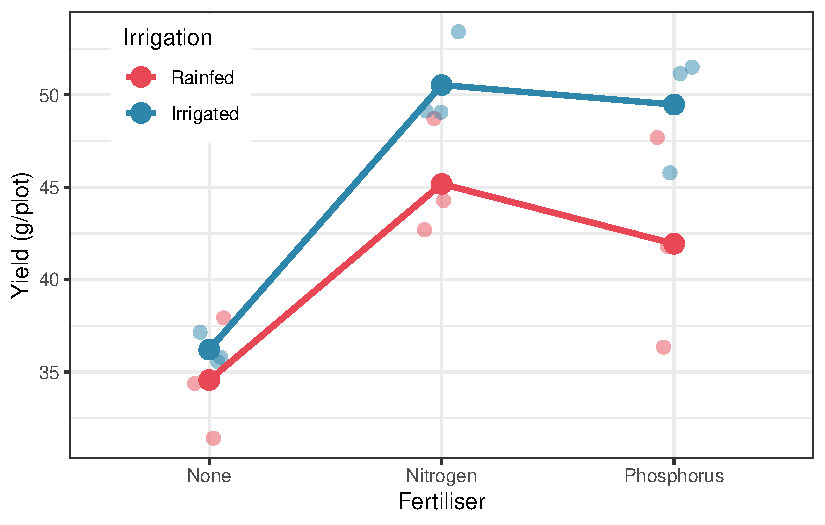
\includegraphics[width=0.9\textwidth,height=\textheight]{03e-split-plot-nested_files/figure-pdf/fig-agriculture-plot-1.pdf}

}

\caption{\label{fig-agriculture-plot}Mean wheat yield by irrigation
regime and fertiliser type in a split-plot design. Points show
individual plot yields. Lines connect the means of each irrigation group
across fertiliser types. The larger spread of the rainfed points
reflects the greater whole-plot variability in unirrigated fields.}

\end{figure}%

\subsection{Why the Split-Plot Analysis
Matters}\label{why-the-split-plot-analysis-matters}

\begin{Shaded}
\begin{Highlighting}[]
\CommentTok{\# Correct split{-}plot analysis vs naive ANOVA}

\CommentTok{\# Correct}
\FunctionTok{cat}\NormalTok{(}\StringTok{"=== Correct split{-}plot analysis ===}\SpecialCharTok{\textbackslash{}n}\StringTok{"}\NormalTok{)}
\end{Highlighting}
\end{Shaded}

\begin{verbatim}
#> === Correct split-plot analysis ===
\end{verbatim}

\begin{Shaded}
\begin{Highlighting}[]
\FunctionTok{print}\NormalTok{(}\FunctionTok{summary}\NormalTok{(fit\_sp))}
\end{Highlighting}
\end{Shaded}

\begin{verbatim}
#> 
#> Error: field
#>            Df Sum Sq Mean Sq F value Pr(>F)
#> irrigation  1  105.6  105.58   3.647  0.129
#> Residuals   4  115.8   28.95               
#> 
#> Error: field:fertiliser
#>                       Df Sum Sq Mean Sq F value   Pr(>F)    
#> fertiliser             2  532.6  266.29  89.801 3.31e-06 ***
#> irrigation:fertiliser  2   26.6   13.28   4.479   0.0495 *  
#> Residuals              8   23.7    2.97                     
#> ---
#> Signif. codes:  0 '***' 0.001 '**' 0.01 '*' 0.05 '.' 0.1 ' ' 1
\end{verbatim}

\begin{Shaded}
\begin{Highlighting}[]
\CommentTok{\# Wrong: treat all plots as independent — ignores field structure}
\FunctionTok{cat}\NormalTok{(}\StringTok{"}\SpecialCharTok{\textbackslash{}n}\StringTok{=== Naive ANOVA (ignoring field structure) ===}\SpecialCharTok{\textbackslash{}n}\StringTok{"}\NormalTok{)}
\end{Highlighting}
\end{Shaded}

\begin{verbatim}
#> 
#> === Naive ANOVA (ignoring field structure) ===
\end{verbatim}

\begin{Shaded}
\begin{Highlighting}[]
\FunctionTok{summary}\NormalTok{(}\FunctionTok{aov}\NormalTok{(yield }\SpecialCharTok{\textasciitilde{}}\NormalTok{ irrigation }\SpecialCharTok{*}\NormalTok{ fertiliser, }\AttributeTok{data =}\NormalTok{ irrig))}
\end{Highlighting}
\end{Shaded}

\begin{verbatim}
#>                       Df Sum Sq Mean Sq F value   Pr(>F)    
#> irrigation             1  105.6  105.58   9.080   0.0108 *  
#> fertiliser             2  532.6  266.29  22.902 8.01e-05 ***
#> irrigation:fertiliser  2   26.6   13.28   1.142   0.3515    
#> Residuals             12  139.5   11.63                     
#> ---
#> Signif. codes:  0 '***' 0.001 '**' 0.01 '*' 0.05 '.' 0.1 ' ' 1
\end{verbatim}

Comparing the two analyses reveals precisely what goes wrong when the
split-plot structure is ignored, and the contrast need all our
attention.

The most consequential difference concerns the irrigation effect. In the
correct split-plot analysis, irrigation is non-significant
(\(F_{1,4} = 3.65\), \(p = 0.129\)), tested against the whole-plot
residual (\(MS = 28.95\)) which is the field-to-field variation that is
the genuine source of uncertainty for a treatment applied at the field
level. In the naive analysis, irrigation appears significant
(\(F_{1,12} = 9.08\), \(p = 0.011\)), tested against the pooled residual
(\(MS = 11.63\)) which combines whole-plot and sub-plot variation
indiscriminately. The naive analysis has produced a false positive: it
declares irrigation significant not because the evidence supports this
conclusion, but because it used an error term that is far too small for
a field-level treatment. The residual degrees of freedom jump from 4 to
12, not because more information is available, but because sub-plot
variation has been illegitimately pressed into service as a stand-in for
whole-plot variation.

The interaction tells an equally instructive story, but in the opposite
direction. In the correct analysis the irrigation-by-fertiliser
interaction is significant (\(F_{2,8} = 4.48\), \(p = 0.049\)), tested
against the sub-plot residual (\(MS = 2.97\)) which is the appropriate
error term for an effect at the plot level. In the naive analysis the
same interaction is non-significant (\(F_{2,12} = 1.14\),
\(p = 0.352\)), because the pooled residual inflates the error term
relative to the true sub-plot noise. Here the naive analysis produces a
false negative: a real interaction that the correct analysis detects is
hidden when the error terms are conflated.

The fertiliser main effect is significant in both analyses and reaches a
similar F value (\(F_{2,8} = 89.80\) vs \(F_{2,12} = 22.90\)), though
the naive analysis underestimates the precision available for sub-plot
comparisons by using a larger pooled residual. This consistency for the
sub-plot factor is not grounds for complacency: the simultaneous false
positive for irrigation and false negative for the interaction show that
the naive analysis gives the right answer for the right factor for the
wrong reasons.

The lesson is general: in a split-plot design, using a single pooled
error term simultaneously makes whole-plot tests too liberal and
sub-plot tests too conservative. \emph{The only correct solution is to
use the two separate error terms that reflect the two levels at which
randomisation actually occurred.}

\part{The Modern Framework}

None of the models we will use in this book are true. But some are
useful. The goal is to use imperfect models to learn about the world ---
carefully, critically, and honestly.

--- Richard McElreath, Statistical Rethinking

\chapter{ANOVA as a Linear Model}\label{sec-chap8}

Part I introduced the idea that ANOVA is a special case of the linear
model i.e.~a regression where the predictors happen to be categorical
rather than continuous. That claim was made quickly and without full
justification, because the tools needed to appreciate it properly had
not yet been developed. Now that you have worked through one-way ANOVA,
multiple comparisons, factorial designs, repeated measures, and
split-plot structures, the time is right to return to this connection
and develop it fully.

This chapter makes the bridge between ANOVA and regression explicit,
concrete, and computable. By the end, you will understand that
\texttt{aov()} and \texttt{lm()} are fitting the same model, that the
choice of coding scheme for categorical predictors determines what the
regression coefficients mean, and that thinking in the linear model
framework rather than in the ANOVA framework opens up a much richer set
of analytical tools.

\section{\texorpdfstring{\texttt{lm()} and \texttt{aov()}: Same Model,
Different
Output}{lm() and aov(): Same Model, Different Output}}\label{lm-and-aov-same-model-different-output}

\subsection{Two Functions, One Model}\label{two-functions-one-model}

R provides two functions for fitting ANOVA-style models: \texttt{aov()}
and \texttt{lm()}. Students often treat them as different tools for
different jobs: \texttt{aov()} for ANOVA and \texttt{lm()} for
regression. This is a \textbf{misconception} worth correcting directly.

Both functions fit exactly the same linear model. They use the same
estimation method (ordinary least squares), the same assumptions, and
the same underlying mathematics. The \textbf{only} difference is in how
they present their output: \texttt{aov()} summarises the fit as an ANOVA
table with sums of squares, degrees of freedom, and F statistics while
\texttt{lm()} summarises the fit as a regression table with coefficient
estimates, standard errors, and t statistics.

The following code fits the same one-way ANOVA model, the fertiliser
experiment from Chapter 3, using both functions and shows that the
fitted values are identical:

\begin{Shaded}
\begin{Highlighting}[]
\FunctionTok{set.seed}\NormalTok{(}\DecValTok{42}\NormalTok{)}

\NormalTok{n }\OtherTok{\textless{}{-}} \DecValTok{20}
\NormalTok{group }\OtherTok{\textless{}{-}} \FunctionTok{factor}\NormalTok{(}\FunctionTok{rep}\NormalTok{(}\FunctionTok{c}\NormalTok{(}\StringTok{"Control"}\NormalTok{, }\StringTok{"Nitrogen"}\NormalTok{, }\StringTok{"Phosphorus"}\NormalTok{), }\AttributeTok{each =}\NormalTok{ n), }\AttributeTok{levels =} \FunctionTok{c}\NormalTok{(}\StringTok{"Control"}\NormalTok{, }\StringTok{"Nitrogen"}\NormalTok{, }\StringTok{"Phosphorus"}\NormalTok{))}
\NormalTok{y }\OtherTok{\textless{}{-}} \FunctionTok{c}\NormalTok{(}\FunctionTok{rnorm}\NormalTok{(n, }\AttributeTok{mean =} \DecValTok{20}\NormalTok{, }\AttributeTok{sd =} \DecValTok{3}\NormalTok{),}
       \FunctionTok{rnorm}\NormalTok{(n, }\AttributeTok{mean =} \DecValTok{25}\NormalTok{, }\AttributeTok{sd =} \DecValTok{3}\NormalTok{),}
       \FunctionTok{rnorm}\NormalTok{(n, }\AttributeTok{mean =} \DecValTok{22}\NormalTok{, }\AttributeTok{sd =} \DecValTok{3}\NormalTok{))}
\NormalTok{df }\OtherTok{\textless{}{-}} \FunctionTok{data.frame}\NormalTok{(y, group)}

\CommentTok{\# Fit with aov()}
\NormalTok{fit\_aov }\OtherTok{\textless{}{-}} \FunctionTok{aov}\NormalTok{(y }\SpecialCharTok{\textasciitilde{}}\NormalTok{ group, }\AttributeTok{data =}\NormalTok{ df)}

\CommentTok{\# Fit with lm()}
\NormalTok{fit\_lm  }\OtherTok{\textless{}{-}} \FunctionTok{lm}\NormalTok{(y }\SpecialCharTok{\textasciitilde{}}\NormalTok{ group,  }\AttributeTok{data =}\NormalTok{ df)}

\CommentTok{\# Are the fitted values identical?}
\CommentTok{\# Are the residuals identical?}
\FunctionTok{cat}\NormalTok{(}
  \StringTok{"Max difference in fitted values:"}\NormalTok{,}
  \FunctionTok{max}\NormalTok{(}\FunctionTok{abs}\NormalTok{(}\FunctionTok{fitted}\NormalTok{(fit\_aov) }\SpecialCharTok{{-}} \FunctionTok{fitted}\NormalTok{(fit\_lm))),}
  \StringTok{"}\SpecialCharTok{\textbackslash{}n}\StringTok{Max difference in residuals:"}\NormalTok{,}
  \FunctionTok{max}\NormalTok{(}\FunctionTok{abs}\NormalTok{(}\FunctionTok{residuals}\NormalTok{(fit\_aov) }\SpecialCharTok{{-}} \FunctionTok{residuals}\NormalTok{(fit\_lm))), }\StringTok{"}\SpecialCharTok{\textbackslash{}n}\StringTok{"}
\NormalTok{  )}
\end{Highlighting}
\end{Shaded}

\begin{verbatim}
#> Max difference in fitted values: 0 
#> Max difference in residuals: 0
\end{verbatim}

Both differences are zero (or within floating-point precision),
confirming that the two functions are producing the same fit. The choice
between them is purely a matter of which output format is more useful
for the question at hand.

\subsection{Reading the Two Outputs Side by
Side}\label{reading-the-two-outputs-side-by-side}

\begin{Shaded}
\begin{Highlighting}[]
\CommentTok{\# ANOVA table output}
\FunctionTok{summary}\NormalTok{(fit\_aov)}
\end{Highlighting}
\end{Shaded}

\begin{verbatim}
#>             Df Sum Sq Mean Sq F value  Pr(>F)   
#> group        2  132.4   66.19   5.513 0.00647 **
#> Residuals   57  684.3   12.01                   
#> ---
#> Signif. codes:  0 '***' 0.001 '**' 0.01 '*' 0.05 '.' 0.1 ' ' 1
\end{verbatim}

\begin{Shaded}
\begin{Highlighting}[]
\CommentTok{\# Regression table output}
\FunctionTok{summary}\NormalTok{(fit\_lm)}
\end{Highlighting}
\end{Shaded}

\begin{verbatim}
#> 
#> Call:
#> lm(formula = y ~ group, data = df)
#> 
#> Residuals:
#>     Min      1Q  Median      3Q     Max 
#> -8.9765 -1.4565  0.2847  2.1828  6.4986 
#> 
#> Coefficients:
#>                 Estimate Std. Error t value Pr(>|t|)    
#> (Intercept)      20.5758     0.7748  26.557  < 2e-16 ***
#> groupNitrogen     3.6113     1.0957   3.296  0.00169 ** 
#> groupPhosphorus   1.4215     1.0957   1.297  0.19974    
#> ---
#> Signif. codes:  0 '***' 0.001 '**' 0.01 '*' 0.05 '.' 0.1 ' ' 1
#> 
#> Residual standard error: 3.465 on 57 degrees of freedom
#> Multiple R-squared:  0.1621, Adjusted R-squared:  0.1327 
#> F-statistic: 5.513 on 2 and 57 DF,  p-value: 0.006473
\end{verbatim}

The ANOVA table answers: does group membership explain a significant
amount of variation in y? The F statistic and its p-value address this
global question.

The regression table answers something more specific: what is the
estimated mean of each group, and how does each group differ from the
reference group? The coefficients and their t statistics address these
pairwise questions directly.

Neither output is more correct: they are complementary views of the same
fitted model. A complete analysis benefits from reading both.

\subsection{\texorpdfstring{Extracting the ANOVA Table from
\texttt{lm()}}{Extracting the ANOVA Table from lm()}}\label{extracting-the-anova-table-from-lm}

The full ANOVA table can be extracted from an \texttt{lm()} fit,
confirming the equivalence explicitly:

\begin{Shaded}
\begin{Highlighting}[]
\CommentTok{\# These produce identical ANOVA tables}
\FunctionTok{anova}\NormalTok{(fit\_lm)}
\end{Highlighting}
\end{Shaded}

\begin{verbatim}
#> Analysis of Variance Table
#> 
#> Response: y
#>           Df Sum Sq Mean Sq F value   Pr(>F)   
#> group      2 132.38  66.190  5.5133 0.006473 **
#> Residuals 57 684.32  12.006                    
#> ---
#> Signif. codes:  0 '***' 0.001 '**' 0.01 '*' 0.05 '.' 0.1 ' ' 1
\end{verbatim}

\begin{Shaded}
\begin{Highlighting}[]
\FunctionTok{summary}\NormalTok{(fit\_aov)}
\end{Highlighting}
\end{Shaded}

\begin{verbatim}
#>             Df Sum Sq Mean Sq F value  Pr(>F)   
#> group        2  132.4   66.19   5.513 0.00647 **
#> Residuals   57  684.3   12.01                   
#> ---
#> Signif. codes:  0 '***' 0.001 '**' 0.01 '*' 0.05 '.' 0.1 ' ' 1
\end{verbatim}

\section{Dummy Coding, Contrast Coding, and What They
Mean}\label{dummy-coding-contrast-coding-and-what-they-mean}

\subsection{The Coding Problem}\label{the-coding-problem}

A linear model requires numerical predictors. When a predictor is
categorical, Control, Nitrogen, Phosphorus, R must convert it to numbers
before fitting the model. The way this conversion is done is called a
\textbf{coding scheme}, and the choice of scheme determines the
interpretation of every coefficient in the model. This is one of the
most frequently misunderstood aspects of linear models in practice.

\subsection{Dummy Coding (Treatment
Coding)}\label{dummy-coding-treatment-coding}

R's default coding for unordered factors is \textbf{dummy coding}, also
called treatment coding. One level is designated the \textbf{reference
level} (by default, the first level alphabetically, in our example here,
Control). For a factor with \(k\) levels, \(k - 1\) binary dummy
variables are created, one for each non-reference level:

\[X_{\text{Nitrogen}} = \begin{cases} 1 & \text{if Nitrogen} \\
0 & \text{otherwise} \end{cases} \qquad
X_{\text{Phosphorus}} = \begin{cases} 1 & \text{if Phosphorus} \\
0 & \text{otherwise} \end{cases}\]

The model is then:

\[y_i = \beta_0 + \beta_1 X_{\text{Nitrogen},i} +
        \beta_2 X_{\text{Phosphorus},i} + \varepsilon_i\]

The coefficients have a direct interpretation:

\begin{itemize}
\tightlist
\item
  \(\beta_0\): the mean of the \textbf{reference group} (Control).
\item
  \(\beta_1\): the difference in means between \textbf{Nitrogen and
  Control}.
\item
  \(\beta_2\): the difference in means between \textbf{Phosphorus and
  Control}.
\end{itemize}

\begin{Shaded}
\begin{Highlighting}[]
\CommentTok{\# R uses dummy coding by default}
\CommentTok{\# Control is the reference level (first alphabetically)}
\FunctionTok{contrasts}\NormalTok{(df}\SpecialCharTok{$}\NormalTok{group)}
\end{Highlighting}
\end{Shaded}

\begin{verbatim}
#>            Nitrogen Phosphorus
#> Control           0          0
#> Nitrogen          1          0
#> Phosphorus        0          1
\end{verbatim}

\begin{Shaded}
\begin{Highlighting}[]
\CommentTok{\# The coefficients reflect this coding}
\FunctionTok{coef}\NormalTok{(fit\_lm)}
\end{Highlighting}
\end{Shaded}

\begin{verbatim}
#>     (Intercept)   groupNitrogen groupPhosphorus 
#>       20.575760        3.611265        1.421508
\end{verbatim}

\begin{Shaded}
\begin{Highlighting}[]
\CommentTok{\# Verify: beta\_0 should equal the Control mean}
\FunctionTok{cat}\NormalTok{(}\StringTok{"Control mean:"}\NormalTok{, }\FunctionTok{mean}\NormalTok{(df}\SpecialCharTok{$}\NormalTok{y[df}\SpecialCharTok{$}\NormalTok{group }\SpecialCharTok{==} \StringTok{"Control"}\NormalTok{]), }\StringTok{"}\SpecialCharTok{\textbackslash{}n}\StringTok{"}\NormalTok{)}
\end{Highlighting}
\end{Shaded}

\begin{verbatim}
#> Control mean: 20.57576
\end{verbatim}

\begin{Shaded}
\begin{Highlighting}[]
\FunctionTok{cat}\NormalTok{(}\StringTok{"Intercept (beta\_0):"}\NormalTok{, }\FunctionTok{coef}\NormalTok{(fit\_lm)[}\DecValTok{1}\NormalTok{], }\StringTok{"}\SpecialCharTok{\textbackslash{}n}\StringTok{"}\NormalTok{)}
\end{Highlighting}
\end{Shaded}

\begin{verbatim}
#> Intercept (beta_0): 20.57576
\end{verbatim}

\begin{Shaded}
\begin{Highlighting}[]
\CommentTok{\# beta\_1 should equal Nitrogen mean minus Control mean}
\FunctionTok{cat}\NormalTok{(}\StringTok{"Nitrogen {-} Control:"}\NormalTok{,}
    \FunctionTok{mean}\NormalTok{(df}\SpecialCharTok{$}\NormalTok{y[df}\SpecialCharTok{$}\NormalTok{group }\SpecialCharTok{==} \StringTok{"Nitrogen"}\NormalTok{]) }\SpecialCharTok{{-}}
    \FunctionTok{mean}\NormalTok{(df}\SpecialCharTok{$}\NormalTok{y[df}\SpecialCharTok{$}\NormalTok{group }\SpecialCharTok{==} \StringTok{"Control"}\NormalTok{]), }\StringTok{"}\SpecialCharTok{\textbackslash{}n}\StringTok{"}\NormalTok{)}
\end{Highlighting}
\end{Shaded}

\begin{verbatim}
#> Nitrogen - Control: 3.611265
\end{verbatim}

\begin{Shaded}
\begin{Highlighting}[]
\FunctionTok{cat}\NormalTok{(}\StringTok{"beta\_1:"}\NormalTok{, }\FunctionTok{coef}\NormalTok{(fit\_lm)[}\DecValTok{2}\NormalTok{], }\StringTok{"}\SpecialCharTok{\textbackslash{}n}\StringTok{"}\NormalTok{)}
\end{Highlighting}
\end{Shaded}

\begin{verbatim}
#> beta_1: 3.611265
\end{verbatim}

As expected, we can see from the above ouput taht \(\beta_0\) exactly
equal the Control mean and \(\beta_1\) equal Nitrogen mean minus Control
mean.

\subsection{Sum-to-Zero Coding (Effects
Coding)}\label{sum-to-zero-coding-effects-coding}

An alternative is \textbf{sum-to-zero coding} (also called effects
coding or deviation coding), where the coefficients represent deviations
from the grand mean rather than differences from a reference group:

\[X_{\text{Nitrogen}} = \begin{cases}
 1 & \text{if Nitrogen} \\ -1 & \text{if Control} \\ 0 & \text{otherwise}
\end{cases} \qquad
X_{\text{Phosphorus}} = \begin{cases}
 1 & \text{if Phosphorus} \\ -1 & \text{if Control} \\ 0 & \text{otherwise}
\end{cases}\]

Under sum-to-zero coding:

\begin{itemize}
\tightlist
\item
  \(\beta_0\): the \textbf{grand mean} (average of all group means).
\item
  \(\beta_1\): the deviation of the \textbf{Nitrogen mean} from the
  grand mean.
\item
  \(\beta_2\): the deviation of the \textbf{Phosphorus mean} from the
  grand mean.
\item
  The Control deviation is \(-(\beta_1 + \beta_2)\), recovered by
  constraint.
\end{itemize}

\begin{Shaded}
\begin{Highlighting}[]
\CommentTok{\# Switch to sum{-}to{-}zero coding}
\FunctionTok{contrasts}\NormalTok{(df}\SpecialCharTok{$}\NormalTok{group) }\OtherTok{\textless{}{-}} \FunctionTok{contr.sum}\NormalTok{(}\DecValTok{3}\NormalTok{)}
\NormalTok{fit\_lm\_sto }\OtherTok{\textless{}{-}} \FunctionTok{lm}\NormalTok{(y }\SpecialCharTok{\textasciitilde{}}\NormalTok{ group, }\AttributeTok{data =}\NormalTok{ df)}
\FunctionTok{coef}\NormalTok{(fit\_lm\_sto)}
\end{Highlighting}
\end{Shaded}

\begin{verbatim}
#> (Intercept)      group1      group2 
#>   22.253351   -1.677591    1.933674
\end{verbatim}

\begin{Shaded}
\begin{Highlighting}[]
\CommentTok{\# Verify: intercept should equal grand mean}
\FunctionTok{cat}\NormalTok{(}\StringTok{"Grand mean:"}\NormalTok{, }\FunctionTok{mean}\NormalTok{(df}\SpecialCharTok{$}\NormalTok{y), }\StringTok{"}\SpecialCharTok{\textbackslash{}n}\StringTok{"}\NormalTok{)}
\end{Highlighting}
\end{Shaded}

\begin{verbatim}
#> Grand mean: 22.25335
\end{verbatim}

\begin{Shaded}
\begin{Highlighting}[]
\FunctionTok{cat}\NormalTok{(}\StringTok{"Intercept (beta\_0):"}\NormalTok{, }\FunctionTok{coef}\NormalTok{(fit\_lm\_sto)[}\DecValTok{1}\NormalTok{], }\StringTok{"}\SpecialCharTok{\textbackslash{}n}\StringTok{"}\NormalTok{)}
\end{Highlighting}
\end{Shaded}

\begin{verbatim}
#> Intercept (beta_0): 22.25335
\end{verbatim}

\begin{Shaded}
\begin{Highlighting}[]
\CommentTok{\# Restore default coding}
\FunctionTok{contrasts}\NormalTok{(df}\SpecialCharTok{$}\NormalTok{group) }\OtherTok{\textless{}{-}} \FunctionTok{contr.treatment}\NormalTok{(}\DecValTok{3}\NormalTok{)}
\end{Highlighting}
\end{Shaded}

Sum-to-zero coding is required for Type III sums of squares (as
discussed in Section~\ref{sec-type3}) and is the natural choice when you
want coefficients that reflect how each group compares to the overall
average rather than to a specific reference group.

\subsection{Helmert Coding}\label{helmert-coding}

\textbf{Helmert coding} compares each level to the average of the
preceding levels. For three groups ordered Control, Nitrogen,
Phosphorus:

\begin{itemize}
\tightlist
\item
  \(\beta_1\): Nitrogen mean minus Control mean.
\item
  \(\beta_2\): Phosphorus mean minus the average of Control and
  Nitrogen.
\end{itemize}

\begin{Shaded}
\begin{Highlighting}[]
\FunctionTok{contrasts}\NormalTok{(df}\SpecialCharTok{$}\NormalTok{group) }\OtherTok{\textless{}{-}} \FunctionTok{contr.helmert}\NormalTok{(}\DecValTok{3}\NormalTok{)}
\NormalTok{fit\_lm\_helm }\OtherTok{\textless{}{-}} \FunctionTok{lm}\NormalTok{(y }\SpecialCharTok{\textasciitilde{}}\NormalTok{ group, }\AttributeTok{data =}\NormalTok{ df)}
\FunctionTok{coef}\NormalTok{(fit\_lm\_helm)}
\end{Highlighting}
\end{Shaded}

\begin{verbatim}
#> (Intercept)      group1      group2 
#>  22.2533508   1.8056323  -0.1280415
\end{verbatim}

\begin{Shaded}
\begin{Highlighting}[]
\CommentTok{\# Restore default}
\FunctionTok{contrasts}\NormalTok{(df}\SpecialCharTok{$}\NormalTok{group) }\OtherTok{\textless{}{-}} \FunctionTok{contr.treatment}\NormalTok{(}\DecValTok{3}\NormalTok{)}
\end{Highlighting}
\end{Shaded}

Helmert coding is useful when the factor levels have a natural
sequential order and you want to test whether each step adds explanatory
power, for example, when comparing a dose-response series or an ordered
treatment hierarchy.

\subsection{\texorpdfstring{The Critical Point: The \(F\) Test Is
Invariant to
Coding}{The Critical Point: The F Test Is Invariant to Coding}}\label{the-critical-point-the-f-test-is-invariant-to-coding}

Whatever coding scheme you choose, the overall \(F\) test for the group
factor, and therefore the ANOVA table, is identical. \textbf{The coding
scheme only changes the interpretation of the individual regression
coefficients, not the global test of whether the groups differ.}

\begin{Shaded}
\begin{Highlighting}[]
\CommentTok{\# All three coding schemes give the same F test}
\FunctionTok{anova}\NormalTok{(}\FunctionTok{lm}\NormalTok{(y }\SpecialCharTok{\textasciitilde{}}\NormalTok{ group, }\AttributeTok{data =}\NormalTok{ df, }\AttributeTok{contrasts =} \FunctionTok{list}\NormalTok{(}\AttributeTok{group =} \FunctionTok{contr.treatment}\NormalTok{(}\DecValTok{3}\NormalTok{))))}
\end{Highlighting}
\end{Shaded}

\begin{verbatim}
#> Analysis of Variance Table
#> 
#> Response: y
#>           Df Sum Sq Mean Sq F value   Pr(>F)   
#> group      2 132.38  66.190  5.5133 0.006473 **
#> Residuals 57 684.32  12.006                    
#> ---
#> Signif. codes:  0 '***' 0.001 '**' 0.01 '*' 0.05 '.' 0.1 ' ' 1
\end{verbatim}

\begin{Shaded}
\begin{Highlighting}[]
\FunctionTok{anova}\NormalTok{(}\FunctionTok{lm}\NormalTok{(y }\SpecialCharTok{\textasciitilde{}}\NormalTok{ group, }\AttributeTok{data =}\NormalTok{ df, }\AttributeTok{contrasts =} \FunctionTok{list}\NormalTok{(}\AttributeTok{group =} \FunctionTok{contr.sum}\NormalTok{(}\DecValTok{3}\NormalTok{))))}
\end{Highlighting}
\end{Shaded}

\begin{verbatim}
#> Analysis of Variance Table
#> 
#> Response: y
#>           Df Sum Sq Mean Sq F value   Pr(>F)   
#> group      2 132.38  66.190  5.5133 0.006473 **
#> Residuals 57 684.32  12.006                    
#> ---
#> Signif. codes:  0 '***' 0.001 '**' 0.01 '*' 0.05 '.' 0.1 ' ' 1
\end{verbatim}

\begin{Shaded}
\begin{Highlighting}[]
\FunctionTok{anova}\NormalTok{(}\FunctionTok{lm}\NormalTok{(y }\SpecialCharTok{\textasciitilde{}}\NormalTok{ group, }\AttributeTok{data =}\NormalTok{ df, }\AttributeTok{contrasts =} \FunctionTok{list}\NormalTok{(}\AttributeTok{group =} \FunctionTok{contr.helmert}\NormalTok{(}\DecValTok{3}\NormalTok{))))}
\end{Highlighting}
\end{Shaded}

\begin{verbatim}
#> Analysis of Variance Table
#> 
#> Response: y
#>           Df Sum Sq Mean Sq F value   Pr(>F)   
#> group      2 132.38  66.190  5.5133 0.006473 **
#> Residuals 57 684.32  12.006                    
#> ---
#> Signif. codes:  0 '***' 0.001 '**' 0.01 '*' 0.05 '.' 0.1 ' ' 1
\end{verbatim}

The sums of squares, \(F\) values, and p-values are identical across all
three. This is a reassuring property: \textbf{your scientific conclusion
about whether groups differ does not depend on an arbitrary choice of
coding scheme}.

\subsection{A Comparison Table}\label{a-comparison-table}

\begin{longtable}[]{@{}
  >{\raggedright\arraybackslash}p{(\columnwidth - 6\tabcolsep) * \real{0.2381}}
  >{\raggedright\arraybackslash}p{(\columnwidth - 6\tabcolsep) * \real{0.2540}}
  >{\raggedright\arraybackslash}p{(\columnwidth - 6\tabcolsep) * \real{0.3016}}
  >{\raggedright\arraybackslash}p{(\columnwidth - 6\tabcolsep) * \real{0.2063}}@{}}
\toprule\noalign{}
\begin{minipage}[b]{\linewidth}\raggedright
Coding scheme
\end{minipage} & \begin{minipage}[b]{\linewidth}\raggedright
Intercept means
\end{minipage} & \begin{minipage}[b]{\linewidth}\raggedright
Coefficients mean
\end{minipage} & \begin{minipage}[b]{\linewidth}\raggedright
When to use
\end{minipage} \\
\midrule\noalign{}
\endhead
\bottomrule\noalign{}
\endlastfoot
Dummy (treatment) & Reference group mean & Difference from reference &
Default; when one group is a natural control \\
Sum-to-zero (effects) & Grand mean & Deviation from grand mean & Type
III SS; no natural reference group \\
Helmert & Weighted grand mean & Sequential comparisons & Ordered levels;
dose-response \\
\end{longtable}

\section{Connecting ANOVA Tables to Regression
Coefficients}\label{connecting-anova-tables-to-regression-coefficients}

\subsection{From Coefficients to Group
Means}\label{from-coefficients-to-group-means}

The regression coefficients and the ANOVA table are two views of the
same fitted model. Understanding the connection between them transforms
the regression output from a set of abstract numbers into a direct
statement about group means.

Under dummy coding, the fitted values (the model's predictions for each
observation) are simply the group means:

\begin{Shaded}
\begin{Highlighting}[]
\CommentTok{\# Fitted values are group means under dummy coding}
\NormalTok{group\_means }\OtherTok{\textless{}{-}} \FunctionTok{tapply}\NormalTok{(df}\SpecialCharTok{$}\NormalTok{y, df}\SpecialCharTok{$}\NormalTok{group, mean)}
\FunctionTok{print}\NormalTok{(group\_means)}
\end{Highlighting}
\end{Shaded}

\begin{verbatim}
#>    Control   Nitrogen Phosphorus 
#>   20.57576   24.18702   21.99727
\end{verbatim}

\begin{Shaded}
\begin{Highlighting}[]
\CommentTok{\# Compare to fitted values from lm()}
\CommentTok{\# All plants in the same group get the same fitted value}
\FunctionTok{head}\NormalTok{(}\FunctionTok{fitted}\NormalTok{(fit\_lm), }\DecValTok{10}\NormalTok{)}
\end{Highlighting}
\end{Shaded}

\begin{verbatim}
#>        1        2        3        4        5        6        7        8 
#> 20.57576 20.57576 20.57576 20.57576 20.57576 20.57576 20.57576 20.57576 
#>        9       10 
#> 20.57576 20.57576
\end{verbatim}

The residuals are the deviations of individual observations from their
group mean which is exactly what we called the within-group variation in
Section~\ref{sec-within-group}.

\subsection{From Sums of Squares to Coefficient
Tests}\label{from-sums-of-squares-to-coefficient-tests}

The \(F\) test in the ANOVA table tests whether all group coefficients
are simultaneously zero i.e.~whether any of
\(\beta_1, \beta_2, \ldots, \beta_{k-1}\) depart from zero. The
individual \(t\) tests in the regression table test each coefficient
separately. These are complementary tests: the \(F\) test is the global
question, the \(t\) tests are the specific pairwise comparisons with the
reference group.

\begin{Shaded}
\begin{Highlighting}[]
\CommentTok{\# The F statistic in the ANOVA table equals the square of the}
\CommentTok{\# t statistic for a two{-}group comparison}
\NormalTok{fit\_two }\OtherTok{\textless{}{-}} \FunctionTok{lm}\NormalTok{(y }\SpecialCharTok{\textasciitilde{}}\NormalTok{ group,}
              \AttributeTok{data =}\NormalTok{ df[df}\SpecialCharTok{$}\NormalTok{group }\SpecialCharTok{\%in\%} \FunctionTok{c}\NormalTok{(}\StringTok{"Control"}\NormalTok{, }\StringTok{"Nitrogen"}\NormalTok{), ],}
              \AttributeTok{contrasts =} \FunctionTok{list}\NormalTok{(}\AttributeTok{group =} \FunctionTok{contr.treatment}\NormalTok{(}\DecValTok{2}\NormalTok{)))}

\NormalTok{t\_val }\OtherTok{\textless{}{-}} \FunctionTok{coef}\NormalTok{(}\FunctionTok{summary}\NormalTok{(fit\_two))[}\StringTok{"group2"}\NormalTok{, }\StringTok{"t value"}\NormalTok{]}
\NormalTok{f\_val }\OtherTok{\textless{}{-}} \FunctionTok{summary}\NormalTok{(}\FunctionTok{aov}\NormalTok{(y }\SpecialCharTok{\textasciitilde{}}\NormalTok{ group,}
                     \AttributeTok{data =}\NormalTok{ df[df}\SpecialCharTok{$}\NormalTok{group }\SpecialCharTok{\%in\%}
                               \FunctionTok{c}\NormalTok{(}\StringTok{"Control"}\NormalTok{, }\StringTok{"Nitrogen"}\NormalTok{), ]))[[}\DecValTok{1}\NormalTok{]][[}\StringTok{"F value"}\NormalTok{]][}\DecValTok{1}\NormalTok{]}

\FunctionTok{cat}\NormalTok{(}
  \StringTok{"t²:"}\NormalTok{, }\FunctionTok{round}\NormalTok{(t\_val}\SpecialCharTok{\^{}}\DecValTok{2}\NormalTok{, }\DecValTok{6}\NormalTok{),}
  \StringTok{"}\SpecialCharTok{\textbackslash{}n}\StringTok{F:"}\NormalTok{, }\FunctionTok{round}\NormalTok{(f\_val, }\DecValTok{6}\NormalTok{), }\StringTok{"}\SpecialCharTok{\textbackslash{}n}\StringTok{"}
\NormalTok{  )}
\end{Highlighting}
\end{Shaded}

\begin{verbatim}
#> t²: 9.809521 
#> F: 9.809521
\end{verbatim}

The \(t\) statistic for a single coefficient squared equals the \(F\)
statistic for the same comparison, confirming that the \(t\) test and
the two-group \(F\) test are the same test expressed differently.

\subsection{Visualising the
Connection}\label{visualising-the-connection}

\begin{Shaded}
\begin{Highlighting}[]
\FunctionTok{library}\NormalTok{(ggplot2)}

\CommentTok{\# Compute group means and CIs from the lm() output}
\NormalTok{pred\_df }\OtherTok{\textless{}{-}} \FunctionTok{data.frame}\NormalTok{(}
  \AttributeTok{group =} \FunctionTok{levels}\NormalTok{(df}\SpecialCharTok{$}\NormalTok{group)}
\NormalTok{)}
\NormalTok{pred\_out }\OtherTok{\textless{}{-}} \FunctionTok{predict}\NormalTok{(fit\_lm, }\AttributeTok{newdata =}\NormalTok{ pred\_df, }\AttributeTok{interval =} \StringTok{"confidence"}\NormalTok{)}
\NormalTok{pred\_df }\OtherTok{\textless{}{-}} \FunctionTok{cbind}\NormalTok{(pred\_df, pred\_out)}
\FunctionTok{names}\NormalTok{(pred\_df) }\OtherTok{\textless{}{-}} \FunctionTok{c}\NormalTok{(}\StringTok{"group"}\NormalTok{, }\StringTok{"mean"}\NormalTok{, }\StringTok{"lwr"}\NormalTok{, }\StringTok{"upr"}\NormalTok{)}

\CommentTok{\# Add coefficient annotations}
\NormalTok{coefs }\OtherTok{\textless{}{-}} \FunctionTok{coef}\NormalTok{(fit\_lm)}
\NormalTok{pred\_df}\SpecialCharTok{$}\NormalTok{label }\OtherTok{\textless{}{-}} \FunctionTok{c}\NormalTok{(}
  \FunctionTok{expression}\NormalTok{(beta[}\DecValTok{0}\NormalTok{]),}
  \FunctionTok{expression}\NormalTok{(beta[}\DecValTok{0}\NormalTok{] }\SpecialCharTok{+}\NormalTok{ beta[}\DecValTok{1}\NormalTok{]),}
  \FunctionTok{expression}\NormalTok{(beta[}\DecValTok{0}\NormalTok{] }\SpecialCharTok{+}\NormalTok{ beta[}\DecValTok{2}\NormalTok{])}
\NormalTok{)}

\FunctionTok{ggplot}\NormalTok{(pred\_df, }\FunctionTok{aes}\NormalTok{(}\AttributeTok{x =}\NormalTok{ group, }\AttributeTok{y =}\NormalTok{ mean, }\AttributeTok{colour =}\NormalTok{ group)) }\SpecialCharTok{+}
  \FunctionTok{geom\_pointrange}\NormalTok{(}\FunctionTok{aes}\NormalTok{(}\AttributeTok{ymin =}\NormalTok{ lwr, }\AttributeTok{ymax =}\NormalTok{ upr), }\AttributeTok{size =} \DecValTok{1}\NormalTok{, }\AttributeTok{linewidth =} \DecValTok{1}\NormalTok{) }\SpecialCharTok{+}
  \FunctionTok{geom\_hline}\NormalTok{(}\AttributeTok{yintercept =}\NormalTok{ coefs[}\DecValTok{1}\NormalTok{], }\AttributeTok{linetype =} \StringTok{"dashed"}\NormalTok{, }\AttributeTok{colour =} \StringTok{"grey50"}\NormalTok{) }\SpecialCharTok{+}
  \FunctionTok{annotate}\NormalTok{(}\StringTok{"text"}\NormalTok{, }\AttributeTok{x =} \FloatTok{0.6}\NormalTok{, }\AttributeTok{y =}\NormalTok{ coefs[}\DecValTok{1}\NormalTok{] }\SpecialCharTok{+} \FloatTok{0.3}\NormalTok{, }\AttributeTok{label =} \FunctionTok{expression}\NormalTok{(beta[}\DecValTok{0}\NormalTok{] }\SpecialCharTok{==} \StringTok{"Control mean"}\NormalTok{), }\AttributeTok{size =} \FloatTok{3.2}\NormalTok{, }\AttributeTok{colour =} \StringTok{"grey40"}\NormalTok{, }\AttributeTok{hjust =} \DecValTok{0}\NormalTok{) }\SpecialCharTok{+}
  \FunctionTok{annotate}\NormalTok{(}\StringTok{"segment"}\NormalTok{, }\AttributeTok{x =} \DecValTok{2}\NormalTok{, }\AttributeTok{xend =} \DecValTok{2}\NormalTok{, }\AttributeTok{y =}\NormalTok{ coefs[}\DecValTok{1}\NormalTok{], }\AttributeTok{yend =}\NormalTok{ coefs[}\DecValTok{1}\NormalTok{] }\SpecialCharTok{+}\NormalTok{ coefs[}\DecValTok{2}\NormalTok{], }\AttributeTok{arrow =} \FunctionTok{arrow}\NormalTok{(}\AttributeTok{length =} \FunctionTok{unit}\NormalTok{(}\FloatTok{0.25}\NormalTok{, }\StringTok{"cm"}\NormalTok{), }\AttributeTok{ends =} \StringTok{"both"}\NormalTok{), }\AttributeTok{colour =} \StringTok{"\#E84855"}\NormalTok{, }\AttributeTok{linewidth =} \FloatTok{0.8}\NormalTok{) }\SpecialCharTok{+}
  \FunctionTok{annotate}\NormalTok{(}\StringTok{"text"}\NormalTok{, }\AttributeTok{x =} \FloatTok{2.1}\NormalTok{, }\AttributeTok{y =}\NormalTok{ coefs[}\DecValTok{1}\NormalTok{] }\SpecialCharTok{+}\NormalTok{ coefs[}\DecValTok{2}\NormalTok{] }\SpecialCharTok{/} \DecValTok{2}\NormalTok{, }\AttributeTok{label =} \FunctionTok{expression}\NormalTok{(beta[}\DecValTok{1}\NormalTok{]), }\AttributeTok{size =} \FloatTok{3.5}\NormalTok{, }\AttributeTok{colour =} \StringTok{"\#E84855"}\NormalTok{, }\AttributeTok{hjust =} \DecValTok{0}\NormalTok{) }\SpecialCharTok{+}
  \FunctionTok{annotate}\NormalTok{(}\StringTok{"segment"}\NormalTok{, }\AttributeTok{x =} \DecValTok{3}\NormalTok{, }\AttributeTok{xend =} \DecValTok{3}\NormalTok{, }\AttributeTok{y =}\NormalTok{ coefs[}\DecValTok{1}\NormalTok{], }\AttributeTok{yend =}\NormalTok{ coefs[}\DecValTok{1}\NormalTok{] }\SpecialCharTok{+}\NormalTok{ coefs[}\DecValTok{3}\NormalTok{], }\AttributeTok{arrow =} \FunctionTok{arrow}\NormalTok{(}\AttributeTok{length =} \FunctionTok{unit}\NormalTok{(}\FloatTok{0.2}\NormalTok{, }\StringTok{"cm"}\NormalTok{), }\AttributeTok{ends =} \StringTok{"both"}\NormalTok{), }\AttributeTok{colour =} \StringTok{"\#F6AE2D"}\NormalTok{, }\AttributeTok{linewidth =} \FloatTok{0.8}\NormalTok{) }\SpecialCharTok{+}
  \FunctionTok{annotate}\NormalTok{(}\StringTok{"text"}\NormalTok{, }\AttributeTok{x =} \FloatTok{3.1}\NormalTok{, }\AttributeTok{y =}\NormalTok{ coefs[}\DecValTok{1}\NormalTok{] }\SpecialCharTok{+}\NormalTok{ coefs[}\DecValTok{3}\NormalTok{] }\SpecialCharTok{/} \DecValTok{2}\NormalTok{, }\AttributeTok{label =} \FunctionTok{expression}\NormalTok{(beta[}\DecValTok{2}\NormalTok{]), }\AttributeTok{size =} \FloatTok{3.5}\NormalTok{, }\AttributeTok{colour =} \StringTok{"\#F6AE2D"}\NormalTok{, }\AttributeTok{hjust =} \DecValTok{0}\NormalTok{) }\SpecialCharTok{+}
  \FunctionTok{scale\_colour\_manual}\NormalTok{(}\AttributeTok{values =} \FunctionTok{c}\NormalTok{(}\StringTok{"\#2E86AB"}\NormalTok{, }\StringTok{"\#E84855"}\NormalTok{, }\StringTok{"\#F6AE2D"}\NormalTok{)) }\SpecialCharTok{+}
  \FunctionTok{labs}\NormalTok{(}\AttributeTok{x =} \ConstantTok{NULL}\NormalTok{, }\AttributeTok{y =} \StringTok{"Plant height (cm)"}\NormalTok{) }\SpecialCharTok{+}
  \FunctionTok{theme\_bw}\NormalTok{() }\SpecialCharTok{+}
  \FunctionTok{theme}\NormalTok{(}\AttributeTok{legend.position =} \StringTok{"none"}\NormalTok{)}
\end{Highlighting}
\end{Shaded}

\begin{figure}[H]

\centering{

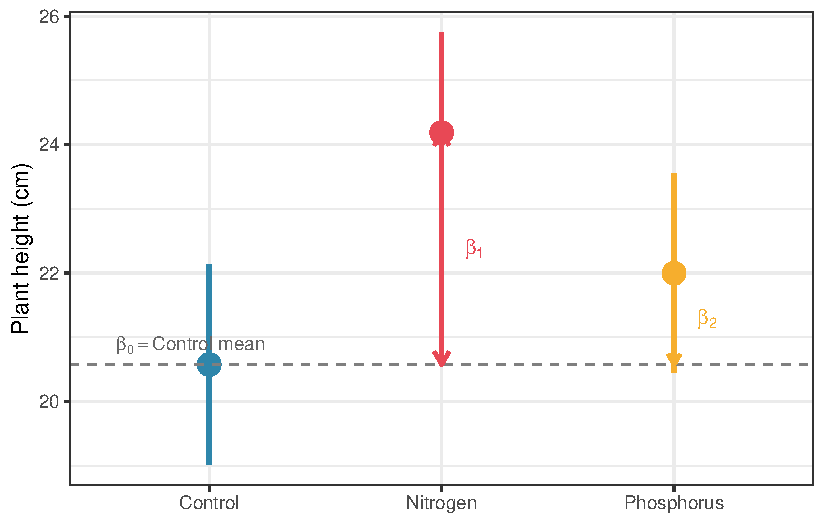
\includegraphics[width=0.9\textwidth,height=\textheight]{04a-anova-as-lm_files/figure-pdf/fig-connection-plot-1.pdf}

}

\caption{\label{fig-connection-plot}The connection between regression
coefficients and ANOVA group means under dummy coding. The intercept
estimates the Control mean; the slope coefficients estimate the
differences between each treatment group and the Control. Error bars
show 95\% confidence intervals for each group mean. Dashed line marks
the Control mean (intercept)}

\end{figure}%

\section{Why Thinking in Linear Models Makes You a Better
Analyst}\label{why-thinking-in-linear-models-makes-you-a-better-analyst}

\subsection{The Limits of the ANOVA
Mindset}\label{the-limits-of-the-anova-mindset}

The ANOVA framework, sums of squares, \(F\) tests, post-hoc comparisons,
is a powerful and well-developed tradition, but it has limits that
become apparent as soon as real data departs from the idealised
conditions of a balanced factorial experiment.

\textbf{ANOVA struggles with continuous covariates.} If you want to test
the effect of fertiliser while adjusting for the initial height of each
plant, ANOVA has no natural way to incorporate that continuous
adjustment. The linear model does: add initial height as a covariate and
the model handles it seamlessly. This is ANCOVA (analysis of covariance)
and it is simply a linear model with both categorical and continuous
predictors.

\textbf{ANOVA struggles with unbalanced designs.} As
Section~\ref{sec-unbalanced} showed, unequal cell sizes create ambiguity
in how sums of squares are computed, requiring careful choices between
Type I, II, and III SS. The linear model has no such ambiguity:
coefficients are estimated by ordinary least squares regardless of
balance, and hypotheses are tested by comparing model fits directly.

\textbf{ANOVA struggles with non-normal responses.} When the response is
a count, a proportion, or a survival time, the normality assumption
\textbf{fails structurally}, not just approximately. The generalised
linear model extends the linear model framework to handle these response
types through a link function and a distributional family. There is no
natural ANOVA equivalent.

\textbf{ANOVA struggles with random effects and hierarchical data.} As
Chapters \textbf{?@sec-repeated} and \textbf{?@sec-split-plot} showed,
repeated measures and nested designs require careful specification of
error terms which a process that becomes unwieldy with more than two
levels of nesting. The linear mixed model handles more seamingly
arbitrarily complex hierarchical structures as a natural extension of
the linear model framework.

\subsection{The Linear Model as a Unifying
Framework}\label{the-linear-model-as-a-unifying-framework}

Every model discussed in this book is a linear model or a direct
extension of one:

\begin{longtable}[]{@{}
  >{\raggedright\arraybackslash}p{(\columnwidth - 2\tabcolsep) * \real{0.2000}}
  >{\raggedright\arraybackslash}p{(\columnwidth - 2\tabcolsep) * \real{0.8000}}@{}}
\toprule\noalign{}
\begin{minipage}[b]{\linewidth}\raggedright
Model
\end{minipage} & \begin{minipage}[b]{\linewidth}\raggedright
Linear model representation
\end{minipage} \\
\midrule\noalign{}
\endhead
\bottomrule\noalign{}
\endlastfoot
One-way ANOVA & \(y = \mu + \alpha_j + \varepsilon\) \\
Two-way ANOVA &
\(y = \mu + \alpha_j + \beta_k + (\alpha\beta)_{jk} + \varepsilon\) \\
ANCOVA & \(y = \mu + \alpha_j + \gamma x + \varepsilon\) \\
Repeated measures & \(y = \mu + \alpha_j + \pi_i + \varepsilon\) \\
Linear mixed model & \(y = X\beta + Zb + \varepsilon\),
\(b \sim \mathcal{N}(0, G)\) \\
Generalised linear model & \(g(\mu) = X\beta\) \\
\end{longtable}

Recognising this unity is not merely intellectually satisfying but has
practical consequences. It means you can use the same diagnostic tools
(residual plots, Q-Q plots, leverage and influence measures) across all
of these models. It means you can compare nested models using likelihood
ratio tests regardless of whether they are ANOVA models, regression
models, or mixed models. And it means you can extend your analyses
naturally as your questions become more complex, rather than switching
to an entirely different analytical tradition every time the data
present a new complication.

\subsection{Model Comparison as a General
Principle}\label{model-comparison-as-a-general-principle}

One of the most powerful tools that the linear model framework provides
is \textbf{model comparison}: testing whether a more complex model fits
the data significantly better than a simpler one. In ANOVA terms, the
\(F\) test is already a model comparison: it compares the model with
group effects to the model without them. But the principle generalises
far beyond the \(F\) test.

\begin{Shaded}
\begin{Highlighting}[]
\CommentTok{\# Model comparison using anova() for nested linear models}
\CommentTok{\# Model 0: no group effect (intercept only)}
\CommentTok{\# Model 1: group effect (one{-}way ANOVA)}
\CommentTok{\# Model 2: group effect plus a continuous covariate}

\FunctionTok{set.seed}\NormalTok{(}\DecValTok{42}\NormalTok{)}
\NormalTok{df}\SpecialCharTok{$}\NormalTok{initial\_height }\OtherTok{\textless{}{-}} \FunctionTok{rnorm}\NormalTok{(}\FunctionTok{nrow}\NormalTok{(df), }\AttributeTok{mean =} \DecValTok{10}\NormalTok{, }\AttributeTok{sd =} \DecValTok{2}\NormalTok{)}

\NormalTok{fit\_m0 }\OtherTok{\textless{}{-}} \FunctionTok{lm}\NormalTok{(y }\SpecialCharTok{\textasciitilde{}} \DecValTok{1}\NormalTok{, }\AttributeTok{data =}\NormalTok{ df)}
\NormalTok{fit\_m1 }\OtherTok{\textless{}{-}} \FunctionTok{lm}\NormalTok{(y }\SpecialCharTok{\textasciitilde{}}\NormalTok{ group, }\AttributeTok{data =}\NormalTok{ df)}
\NormalTok{fit\_m2 }\OtherTok{\textless{}{-}} \FunctionTok{lm}\NormalTok{(y }\SpecialCharTok{\textasciitilde{}}\NormalTok{ group }\SpecialCharTok{+}\NormalTok{ initial\_height, }\AttributeTok{data =}\NormalTok{ df)}

\CommentTok{\# Sequential model comparison}
\FunctionTok{anova}\NormalTok{(fit\_m0, fit\_m1, fit\_m2)}
\end{Highlighting}
\end{Shaded}

\begin{verbatim}
#> Analysis of Variance Table
#> 
#> Model 1: y ~ 1
#> Model 2: y ~ group
#> Model 3: y ~ group + initial_height
#>   Res.Df    RSS Df Sum of Sq          F    Pr(>F)    
#> 1     59 816.70                                      
#> 2     57 684.32  2    132.38 1.1525e+30 < 2.2e-16 ***
#> 3     56   0.00  1    684.32 1.1916e+31 < 2.2e-16 ***
#> ---
#> Signif. codes:  0 '***' 0.001 '**' 0.01 '*' 0.05 '.' 0.1 ' ' 1
\end{verbatim}

The output shows, for each step, whether adding the new term
significantly improves the fit. This is the same logic as the ANOVA
\(F\) test, but applied sequentially across a series of models of
increasing complexity. It is a general and flexible tool that works for
any combination of categorical and continuous predictors.

\subsection{A Practical
Recommendation}\label{a-practical-recommendation}

The practical implication of everything in this chapter is simple:
\textbf{fit your models with \texttt{lm()} and use \texttt{anova()} or
\texttt{car::Anova()} to extract the ANOVA table when you need it},
rather than treating \texttt{aov()} as a separate tool for a separate
job. The \texttt{lm()} workflow gives you access to the full suite of
linear model diagnostics, coefficient plots, model comparison tools, and
extensions to ANCOVA and mixed models, none of which are as naturally
available from \texttt{aov()}.

The one exception is complex error-term specifications that can arise
for split-plot and repeated measures designs that require explicit
\texttt{Error()} terms. For these, \texttt{aov()} remains convenient,
though as Part III will show, linear mixed models handle the same
structures more flexibly and with fewer constraints.

The ANOVA table is a useful summary. The linear model is the foundation.
Keeping this distinction clear will serve you well as your analyses
become more complex.

\chapter{Mixed-Effects Models: Beyond Classical ANOVA}\label{sec-chap9}

The repeated measures and split-plot designs of Chapters
\textbf{?@sec-repeated} and \textbf{?@sec-split-plot} introduced the
idea that not all sources of variation in biological data are equal.
Some variation is systematic and of direct scientific interest like the
effect of a treatment, a drug, a genotype. Some variation is structural
and must be accounted for but is not itself the focus like the fact that
patients differ from one another, that plots within the same field are
more similar than plots in different fields, that repeated measurements
on the same individual are correlated.

Classical ANOVA handles these structural sources of variation through
explicit error terms like the \texttt{Error()} specification in
\texttt{aov()}. This works well for simple, balanced designs with one or
two levels of nesting. It becomes unwieldy, and eventually impossible,
when the hierarchical structure is more complex, when data are missing,
when the design is unbalanced, or when you want to make inferences that
generalise beyond the specific levels of a grouping factor that happen
to appear in your data.

Mixed-effects models are the modern solution to all of these problems.
They extend the linear model framework by including both \textbf{fixed
effects}, the systematic, estimable treatment effects that classical
ANOVA tests, and \textbf{random effects}, the structural variation
attributable to grouping factors whose levels are a random sample from a
larger population. The result is a framework that is simultaneously more
flexible, more honest about the structure of biological data, and more
directly connected to the scientific questions being asked.

\section{When Random Effects Are
Necessary}\label{when-random-effects-are-necessary}

\subsection{The Three Situations That Demand Random
Effects}\label{the-three-situations-that-demand-random-effects}

Random effects are not merely a statistical convenience, they are the
correct model for specific, recognisable data structures. Three
situations arise repeatedly in biological research where failing to
include random effects leads directly to incorrect inference.

\textbf{Situation 1: Clustered observations.} Measurements taken on
units that belong to the same higher-level group will be more similar to
each other than measurements from different groups, regardless of any
treatment. Patients recruited from the same hospital share clinical
practices, patient population, and staffing. Plants in the same
greenhouse bench share light and temperature. Students in the same
classroom share a teacher. This within-cluster similarity, quantified by
the intraclass correlation coefficient introduced in Section 2.6, means
the observations are not independent, and the effective sample size is
smaller than the raw count of observations suggests. A random effect for
the cluster absorbs this similarity and produces correct standard
errors.

\textbf{Situation 2: Repeated measurements.} When the same individual is
measured multiple times at different time points, under different
conditions, or in different locations, the repeated measurements on the
same individual are correlated. Chapter \textbf{?@sec-repeated} handled
this with repeated measures ANOVA. Mixed models handle it more flexibly:
the individual is modelled as a random effect, and the covariance
structure of the repeated measurements can be specified explicitly.
Mixed models also handle missing data gracefully, which repeated
measures ANOVA cannot.

\textbf{Situation 3: Generalising beyond the observed levels.} If the
levels of a grouping factor in your study are a random sample from a
larger population like hospitals drawn from a healthcare system, farms
drawn from a region or batches drawn from a production run and you want
your conclusions to generalise to that larger population, the grouping
factor must be treated as random. A fixed effect estimates the mean of
each specific level observed; a random effect estimates the distribution
of levels in the population.

\subsection{Recognising Random Effects in
Practice}\label{recognising-random-effects-in-practice}

The practical question is: for each grouping factor in your data, are
the levels the specific entities of interest, or a sample representing a
broader population?

\begin{longtable}[]{@{}
  >{\raggedright\arraybackslash}p{(\columnwidth - 4\tabcolsep) * \real{0.2424}}
  >{\raggedright\arraybackslash}p{(\columnwidth - 4\tabcolsep) * \real{0.5152}}
  >{\raggedright\arraybackslash}p{(\columnwidth - 4\tabcolsep) * \real{0.2424}}@{}}
\toprule\noalign{}
\begin{minipage}[b]{\linewidth}\raggedright
Factor
\end{minipage} & \begin{minipage}[b]{\linewidth}\raggedright
Fixed or random?
\end{minipage} & \begin{minipage}[b]{\linewidth}\raggedright
Reason
\end{minipage} \\
\midrule\noalign{}
\endhead
\bottomrule\noalign{}
\endlastfoot
Fertiliser type (control, N, P) & Fixed & Specific treatments of
interest \\
Hospital (12 of 200 in region) & Random & Sample from a population \\
Patient (20 recruited volunteers) & Random & Sample from a population \\
Genotype (4 specific varieties) & Fixed & Specific varieties of
interest \\
Field (6 randomly selected) & Random & Sample from a population \\
Time point (weeks 0, 4, 8, 12) & Fixed & Specific times of interest \\
\end{longtable}

When in doubt, ask: \textbf{would you want your conclusions to apply to
levels of this factor that were not in your study?} If yes, the factor
is random.

\section{Random Intercepts and Random
Slopes}\label{random-intercepts-and-random-slopes}

\subsection{The Random Intercept
Model}\label{the-random-intercept-model}

The simplest mixed model adds a random intercept for each level of a
grouping factor. For a study with patients nested within hospitals, the
random intercept model is:

\[y_{ij} = \underbrace{\beta_0 + \beta_1 x_{ij}}_{\text{fixed effects}} +
           \underbrace{b_j}_{\text{random intercept}} +
           \underbrace{\varepsilon_{ij}}_{\text{residual}}\]

where \(y_{ij}\) is the response for patient \(i\) in hospital \(j\),
\(x_{ij}\) is a predictor (treatment, time, covariate), \(b_j\) is the
random intercept for hospital \(j\), and \(\varepsilon_{ij}\) is the
residual. The random intercepts are assumed normally distributed:

\[b_j \sim \mathcal{N}(0, \sigma^2_b)\]

The random intercept \(b_j\) captures the fact that some hospitals have
systematically higher or lower outcomes than average, for reasons
unrelated to the treatment being studied. By modelling this explicitly,
the fixed effect \(\beta_1\) is estimated after accounting for
hospital-level differences which is a more honest and more precise
estimate than one that ignores the clustering.

\subsection{The Random Slope Model}\label{the-random-slope-model}

A \textbf{random intercept} allows each group to have a different
baseline level of the response. A \textbf{random slope} allows each
group to have a different relationship between a predictor and the
response:

\[y_{ij} = (\beta_0 + b_{0j}) + (\beta_1 + b_{1j}) x_{ij} +
           \varepsilon_{ij}\]

where \(b_{0j}\) is the random intercept for group \(j\) and \(b_{1j}\)
is the random slope i.e.~the deviation of group \(j\)'s slope from the
average slope \(\beta_1\). Together they form a bivariate normal
distribution:

\[\begin{pmatrix} b_{0j} \\ b_{1j} \end{pmatrix} \sim
  \mathcal{N}\left(
    \begin{pmatrix} 0 \\ 0 \end{pmatrix},
    \begin{pmatrix} \sigma^2_0 & \sigma_{01} \\
                    \sigma_{01} & \sigma^2_1 \end{pmatrix}
  \right)\]

The covariance \(\sigma_{01}\) captures whether groups that start higher
also tend to change more (or less) rapidly, an estimate that is a
biologically important quantity in longitudinal studies.

\subsection{Visualising Random Intercepts and
Slopes}\label{visualising-random-intercepts-and-slopes}

\begin{Shaded}
\begin{Highlighting}[]
\FunctionTok{library}\NormalTok{(ggplot2)}
\FunctionTok{library}\NormalTok{(patchwork)}

\FunctionTok{set.seed}\NormalTok{(}\DecValTok{42}\NormalTok{)}

\NormalTok{n\_groups }\OtherTok{\textless{}{-}} \DecValTok{8}
\NormalTok{n\_obs }\OtherTok{\textless{}{-}} \DecValTok{10}
\NormalTok{x }\OtherTok{\textless{}{-}} \FunctionTok{seq}\NormalTok{(}\DecValTok{0}\NormalTok{, }\DecValTok{1}\NormalTok{, }\AttributeTok{length.out =}\NormalTok{ n\_obs)}

\CommentTok{\# Random intercept model}
\NormalTok{ri\_data }\OtherTok{\textless{}{-}} \FunctionTok{do.call}\NormalTok{(rbind, }\FunctionTok{lapply}\NormalTok{(}\FunctionTok{seq\_len}\NormalTok{(n\_groups), }\ControlFlowTok{function}\NormalTok{(g) \{}
\NormalTok{  b0 }\OtherTok{\textless{}{-}} \FunctionTok{rnorm}\NormalTok{(}\DecValTok{1}\NormalTok{, }\DecValTok{0}\NormalTok{, }\DecValTok{2}\NormalTok{)}
  \FunctionTok{data.frame}\NormalTok{(}
    \AttributeTok{x =}\NormalTok{ x,}
    \AttributeTok{y =} \DecValTok{3} \SpecialCharTok{+}\NormalTok{ b0 }\SpecialCharTok{+} \DecValTok{2} \SpecialCharTok{*}\NormalTok{ x }\SpecialCharTok{+} \FunctionTok{rnorm}\NormalTok{(n\_obs, }\DecValTok{0}\NormalTok{, }\FloatTok{0.5}\NormalTok{),}
    \AttributeTok{group =} \FunctionTok{factor}\NormalTok{(g)}
\NormalTok{  )}
\NormalTok{\}))}

\CommentTok{\# Random slope model}
\NormalTok{rs\_data }\OtherTok{\textless{}{-}} \FunctionTok{do.call}\NormalTok{(rbind, }\FunctionTok{lapply}\NormalTok{(}\FunctionTok{seq\_len}\NormalTok{(n\_groups), }\ControlFlowTok{function}\NormalTok{(g) \{}
\NormalTok{  b0 }\OtherTok{\textless{}{-}} \FunctionTok{rnorm}\NormalTok{(}\DecValTok{1}\NormalTok{, }\DecValTok{0}\NormalTok{, }\DecValTok{2}\NormalTok{)}
\NormalTok{  b1 }\OtherTok{\textless{}{-}} \FunctionTok{rnorm}\NormalTok{(}\DecValTok{1}\NormalTok{, }\DecValTok{0}\NormalTok{, }\FloatTok{1.5}\NormalTok{)}
  \FunctionTok{data.frame}\NormalTok{(}
    \AttributeTok{x =}\NormalTok{ x,}
    \AttributeTok{y =} \DecValTok{3} \SpecialCharTok{+}\NormalTok{ b0 }\SpecialCharTok{+}\NormalTok{ (}\DecValTok{2} \SpecialCharTok{+}\NormalTok{ b1) }\SpecialCharTok{*}\NormalTok{ x }\SpecialCharTok{+} \FunctionTok{rnorm}\NormalTok{(n\_obs, }\DecValTok{0}\NormalTok{, }\FloatTok{0.5}\NormalTok{),}
    \AttributeTok{group =} \FunctionTok{factor}\NormalTok{(g)}
\NormalTok{  )}
\NormalTok{\}))}

\NormalTok{p1 }\OtherTok{\textless{}{-}} \FunctionTok{ggplot}\NormalTok{(ri\_data, }\FunctionTok{aes}\NormalTok{(}\AttributeTok{x =}\NormalTok{ x, }\AttributeTok{y =}\NormalTok{ y, }\AttributeTok{group =}\NormalTok{ group)) }\SpecialCharTok{+}
  \FunctionTok{geom\_line}\NormalTok{(}\AttributeTok{colour =} \StringTok{"\#2E86AB"}\NormalTok{, }\AttributeTok{alpha =} \FloatTok{0.5}\NormalTok{) }\SpecialCharTok{+}
  \FunctionTok{geom\_abline}\NormalTok{(}\AttributeTok{intercept =} \DecValTok{3}\NormalTok{, }\AttributeTok{slope =} \DecValTok{2}\NormalTok{,}
              \AttributeTok{linetype =} \StringTok{"dashed"}\NormalTok{, }\AttributeTok{colour =} \StringTok{"grey30"}\NormalTok{,}
              \AttributeTok{linewidth =} \FloatTok{1.2}\NormalTok{) }\SpecialCharTok{+}
  \FunctionTok{labs}\NormalTok{(}\AttributeTok{x =} \StringTok{"Time"}\NormalTok{, }\AttributeTok{y =} \StringTok{"Response"}\NormalTok{) }\SpecialCharTok{+}
  \FunctionTok{theme\_bw}\NormalTok{()}

\NormalTok{p2 }\OtherTok{\textless{}{-}} \FunctionTok{ggplot}\NormalTok{(rs\_data, }\FunctionTok{aes}\NormalTok{(}\AttributeTok{x =}\NormalTok{ x, }\AttributeTok{y =}\NormalTok{ y, }\AttributeTok{group =}\NormalTok{ group)) }\SpecialCharTok{+}
  \FunctionTok{geom\_line}\NormalTok{(}\AttributeTok{colour =} \StringTok{"\#E84855"}\NormalTok{, }\AttributeTok{alpha =} \FloatTok{0.5}\NormalTok{) }\SpecialCharTok{+}
  \FunctionTok{geom\_abline}\NormalTok{(}\AttributeTok{intercept =} \DecValTok{3}\NormalTok{, }\AttributeTok{slope =} \DecValTok{2}\NormalTok{,}
              \AttributeTok{linetype =} \StringTok{"dashed"}\NormalTok{, }\AttributeTok{colour =} \StringTok{"grey30"}\NormalTok{,}
              \AttributeTok{linewidth =} \FloatTok{1.2}\NormalTok{) }\SpecialCharTok{+}
  \FunctionTok{labs}\NormalTok{(}\AttributeTok{x =} \StringTok{"Time"}\NormalTok{, }\AttributeTok{y =} \StringTok{"Response"}\NormalTok{) }\SpecialCharTok{+}
  \FunctionTok{theme\_bw}\NormalTok{()}

\NormalTok{p1 }\SpecialCharTok{+}\NormalTok{ p2}
\end{Highlighting}
\end{Shaded}

\begin{figure}[H]

\centering{

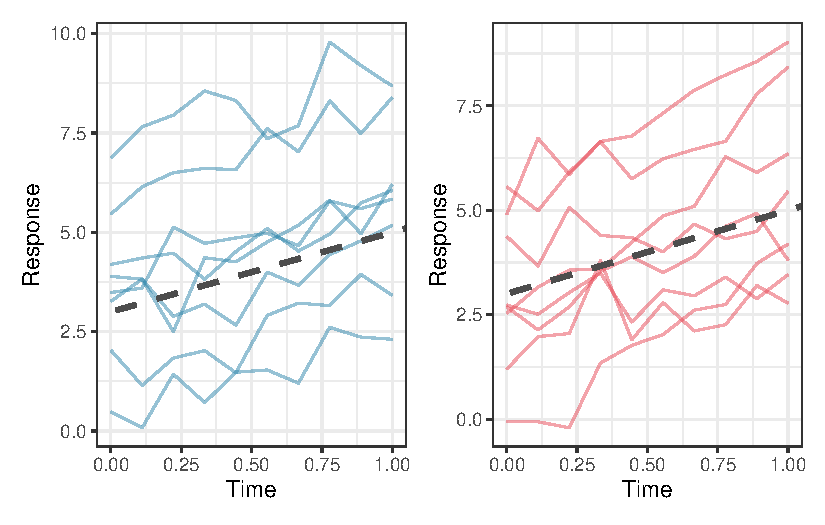
\includegraphics[width=0.9\textwidth,height=\textheight]{04b-mixed-effects_files/figure-pdf/fig-random-effects-plot-1.pdf}

}

\caption{\label{fig-random-effects-plot}Left: a random intercept model,
all groups share the same slope but have different intercepts. The
dashed line is the population-level (fixed effect) trajectory; solid
lines are group-specific trajectories. Right: a random slope model,
groups differ in both their starting level and their rate of change. The
variation in slopes is itself a scientifically meaningful quantity.}

\end{figure}%

\subsection{Choosing Between Random Intercepts and Random
Slopes}\label{choosing-between-random-intercepts-and-random-slopes}

The choice between a random intercept model and a random slope model is
not merely statistical but it reflects a scientific question. A random
intercept model asks: do groups differ in their average response level?
A random slope model asks additionally: do groups differ in how the
response changes with the predictor?

In a clinical trial measuring recovery over time, a random intercept
captures the fact that some patients start sicker than others. A random
slope captures the additional possibility that some patients improve
faster than others which is a clinically important question about
treatment response heterogeneity.

Include a random slope when you have scientific reason to believe that
the relationship between the predictor and the response genuinely varies
across groups, and you got enough data to estimate the additional
variance component reliably.

As a practical guide, at least 5-6 groups are needed to estimate a
random intercept variance reliably, and at least 10-15 groups for a
random intercept plus slope model. With fewer groups, the variance
estimates will be unstable and the model may fail to converge.

\section{\texorpdfstring{\texttt{lme4} and \texttt{nlme}: A Practical
Guide}{lme4 and nlme: A Practical Guide}}\label{lme4-and-nlme-a-practical-guide}

\subsection{Two Packages, Different
Strengths}\label{two-packages-different-strengths}

Two R packages dominate mixed-effects modelling in biology:
\texttt{lme4} \citep{Bates2015} and \texttt{nlme} \citep{Pinheiro2000}.
They fit the same broad class of models but differ in their syntax,
capabilities, and defaults.

\textbf{\texttt{lme4}} is the modern standard for most applications. It
is fast, handles crossed and nested random effects naturally, and uses a
clean formula syntax. Its main limitation is that it does not directly
provide p-values for fixed effects which is a deliberate design decision
by its authors that reflects genuine statistical controversy (see
Section 9.4).

\textbf{\texttt{nlme}} is older but offers features that \texttt{lme4}
does not: direct specification of residual covariance structures (useful
for repeated measures with heterogeneous variances) and nonlinear mixed
models. Its syntax is more verbose and it handles crossed random effects
less elegantly than \texttt{lme4}.

For most applications in this book, \texttt{lme4} is the right choice.

\subsection{\texorpdfstring{The \texttt{lme4} Formula
Syntax}{The lme4 Formula Syntax}}\label{the-lme4-formula-syntax}

\texttt{lme4} extends R's standard model formula with a notation for
random effects: \texttt{(random\_effect\ \textbar{}\ grouping\_factor)}.
The vertical bar \texttt{\textbar{}} separates the random effect
structure from the grouping factor.

\begin{longtable}[]{@{}
  >{\raggedright\arraybackslash}p{(\columnwidth - 2\tabcolsep) * \real{0.5625}}
  >{\raggedright\arraybackslash}p{(\columnwidth - 2\tabcolsep) * \real{0.4375}}@{}}
\toprule\noalign{}
\begin{minipage}[b]{\linewidth}\raggedright
Formula
\end{minipage} & \begin{minipage}[b]{\linewidth}\raggedright
Model
\end{minipage} \\
\midrule\noalign{}
\endhead
\bottomrule\noalign{}
\endlastfoot
\texttt{y\ \textasciitilde{}\ x\ +\ (1\ \textbar{}\ group)} & Fixed
slope for x; random intercept by group \\
\texttt{y\ \textasciitilde{}\ x\ +\ (x\ \textbar{}\ group)} & Fixed
slope for x; random intercept and slope by group \\
\texttt{y\ \textasciitilde{}\ x\ +\ (1\ \textbar{}\ group)\ +\ (1\ \textbar{}\ block)}
& Two crossed random effects \\
\texttt{y\ \textasciitilde{}\ x\ +\ (1\ \textbar{}\ region/hospital)} &
Hospital nested within region \\
\texttt{y\ \textasciitilde{}\ x\ +\ (1\ \textbar{}\ region)\ +\ (1\ \textbar{}\ region:hospital)}
& Equivalent nested specification \\
\end{longtable}

\subsection{Fitting and Interpreting a Random Intercept
Model}\label{sec-rim}

\begin{Shaded}
\begin{Highlighting}[]
\FunctionTok{library}\NormalTok{(lme4)}
\end{Highlighting}
\end{Shaded}

\begin{verbatim}
#> Loading required package: Matrix
\end{verbatim}

\begin{Shaded}
\begin{Highlighting}[]
\FunctionTok{set.seed}\NormalTok{(}\DecValTok{42}\NormalTok{)}

\CommentTok{\# Simulate a simple random intercept dataset}
\CommentTok{\# 20 patients per hospital, 10 hospitals, one treatment covariate}
\NormalTok{n\_hospitals }\OtherTok{\textless{}{-}} \DecValTok{10}
\NormalTok{n\_patients  }\OtherTok{\textless{}{-}} \DecValTok{20}
\NormalTok{hospital\_sd }\OtherTok{\textless{}{-}} \DecValTok{3}
\NormalTok{patient\_sd  }\OtherTok{\textless{}{-}} \DecValTok{2}

\NormalTok{df\_lme }\OtherTok{\textless{}{-}} \FunctionTok{do.call}\NormalTok{(rbind, }\FunctionTok{lapply}\NormalTok{(}\FunctionTok{seq\_len}\NormalTok{(n\_hospitals), }\ControlFlowTok{function}\NormalTok{(h) \{}
\NormalTok{  hospital\_effect }\OtherTok{\textless{}{-}} \FunctionTok{rnorm}\NormalTok{(}\DecValTok{1}\NormalTok{, }\DecValTok{0}\NormalTok{, hospital\_sd)}
  \FunctionTok{data.frame}\NormalTok{(}
    \AttributeTok{outcome =} \FunctionTok{rnorm}\NormalTok{(n\_patients, }\AttributeTok{mean =} \DecValTok{50} \SpecialCharTok{+}\NormalTok{ hospital\_effect }\SpecialCharTok{+}
                             \DecValTok{2} \SpecialCharTok{*} \FunctionTok{rbinom}\NormalTok{(n\_patients, }\DecValTok{1}\NormalTok{, }\FloatTok{0.5}\NormalTok{),}
                      \AttributeTok{sd   =}\NormalTok{ patient\_sd),}
    \AttributeTok{treatment =} \FunctionTok{factor}\NormalTok{(}\FunctionTok{rep}\NormalTok{(}\FunctionTok{c}\NormalTok{(}\StringTok{"Control"}\NormalTok{, }\StringTok{"Treatment"}\NormalTok{), }\AttributeTok{each =}\NormalTok{ n\_patients }\SpecialCharTok{/} \DecValTok{2}\NormalTok{)),}
    \AttributeTok{hospital =} \FunctionTok{factor}\NormalTok{(h)}
\NormalTok{  )}
\NormalTok{\}))}

\CommentTok{\# Fit random intercept model}
\NormalTok{fit\_ri }\OtherTok{\textless{}{-}}\NormalTok{ lme4}\SpecialCharTok{::}\FunctionTok{lmer}\NormalTok{(outcome }\SpecialCharTok{\textasciitilde{}}\NormalTok{ treatment }\SpecialCharTok{+}\NormalTok{ (}\DecValTok{1} \SpecialCharTok{|}\NormalTok{ hospital), }\AttributeTok{data =}\NormalTok{ df\_lme, }\AttributeTok{REML =} \ConstantTok{TRUE}\NormalTok{)}
\FunctionTok{summary}\NormalTok{(fit\_ri)}
\end{Highlighting}
\end{Shaded}

\begin{verbatim}
#> Linear mixed model fit by REML ['lmerMod']
#> Formula: outcome ~ treatment + (1 | hospital)
#>    Data: df_lme
#> 
#> REML criterion at convergence: 897.6
#> 
#> Scaled residuals: 
#>     Min      1Q  Median      3Q     Max 
#> -2.8980 -0.6451  0.0198  0.5870  3.3917 
#> 
#> Random effects:
#>  Groups   Name        Variance Std.Dev.
#>  hospital (Intercept) 5.609    2.368   
#>  Residual             4.486    2.118   
#> Number of obs: 200, groups:  hospital, 10
#> 
#> Fixed effects:
#>                    Estimate Std. Error t value
#> (Intercept)         52.8446     0.7783  67.895
#> treatmentTreatment   0.2663     0.2995   0.889
#> 
#> Correlation of Fixed Effects:
#>             (Intr)
#> trtmntTrtmn -0.192
\end{verbatim}

The summary output has four sections worth reading carefully.

\textbf{Random effects:} the variance components. \texttt{(Intercept)}
under \texttt{hospital} is \(\hat{\sigma}^2_b\): the estimated variance
in baseline outcomes across hospitals. \texttt{Residual} is
\(\hat{\sigma}^2_\varepsilon\): the within-hospital, within-patient
variation. Their ratio tells you how much of the total variation is
attributable to hospital-level differences. From the result, the
intraclass correlation is therefore
\(\text{ICC} = 5.61 / (5.61 + 4.49) = 0.56\), meaning that 56\% of the
total variation in outcomes is attributable to systematic differences
between hospitals which a substantial clustering effect that would badly
distort any analysis that ignored it.

\textbf{Fixed effects:} the coefficient table. The \texttt{(Intercept)}
is the estimated mean outcome in the reference group (Control) at an
average hospital. The treatment coefficient (here
\texttt{treatmentTreatment}) is the estimated average difference between
treatment and control, after accounting for hospital-level variation.

\textbf{Correlation of fixed effects:} the correlation between the
intercept and treatment coefficient estimates. Large correlations (close
to ±1) can indicate collinearity or model specification problems.

\textbf{Number of observations and groups:} always verify these match
your data. Here 200 observations are nested in 10 hospitals, 20 patients
per hospital, as specified. A mismatch between these numbers and your
intended design is the first sign of a coding error in the grouping
factor.

\subsection{REML vs ML Estimation}\label{sec-reml-ml}

\texttt{lme4} offers two estimation methods, controlled by the
\texttt{REML} argument:

\textbf{REML (Restricted Maximum Likelihood)} is the default
(\texttt{REML\ =\ TRUE})and should be used when the goal is to estimate
variance components. REML produces unbiased estimates of \(\sigma^2_b\)
and \(\sigma^2_\varepsilon\), analogous to dividing by \(n-1\) rather
than \(n\) when estimating a variance.

\textbf{ML (Maximum Likelihood)} should be used
(\texttt{REML\ =\ FALSE}) when comparing models with different fixed
effect structures using likelihood ratio tests. REML likelihoods are not
comparable across models with different fixed effects because they are
computed on different effective datasets.

The practical workflow is therefore always two steps: use
\texttt{REML\ =\ FALSE} to compare models and identify which fixed
effects belong in the model, then refit the winning model with
\texttt{REML\ =\ TRUE} to obtain the final, unbiased variance component
estimates for reporting.

\begin{Shaded}
\begin{Highlighting}[]
\CommentTok{\# Step 1: fit both models with ML = FALSE to enable}
\CommentTok{\# a valid likelihood ratio test comparing their fixed effects.}
\CommentTok{\# REML = FALSE is mandatory here. Comparing REML likelihoods}
\CommentTok{\# across models with different fixed effects is not valid.}
\NormalTok{fit\_ri\_ml   }\OtherTok{\textless{}{-}}\NormalTok{ lme4}\SpecialCharTok{::}\FunctionTok{lmer}\NormalTok{(outcome }\SpecialCharTok{\textasciitilde{}}\NormalTok{ treatment }\SpecialCharTok{+}\NormalTok{ (}\DecValTok{1} \SpecialCharTok{|}\NormalTok{ hospital), }\AttributeTok{data =}\NormalTok{ df\_lme, }\AttributeTok{REML =} \ConstantTok{FALSE}\NormalTok{)}
\NormalTok{fit\_null\_ml }\OtherTok{\textless{}{-}}\NormalTok{ lme4}\SpecialCharTok{::}\FunctionTok{lmer}\NormalTok{(outcome }\SpecialCharTok{\textasciitilde{}} \DecValTok{1} \SpecialCharTok{+}\NormalTok{ (}\DecValTok{1} \SpecialCharTok{|}\NormalTok{ hospital), }\AttributeTok{data =}\NormalTok{ df\_lme, }\AttributeTok{REML =} \ConstantTok{FALSE}\NormalTok{)}

\CommentTok{\# Likelihood ratio test: does adding treatment improve the fit?}
\CommentTok{\# The chi{-}squared statistic is {-}2 * (logLik(null) {-} logLik(full))}
\CommentTok{\# with degrees of freedom equal to the difference in parameters.}
\FunctionTok{anova}\NormalTok{(fit\_null\_ml, fit\_ri\_ml)}
\end{Highlighting}
\end{Shaded}

\begin{verbatim}
#> Data: df_lme
#> Models:
#> fit_null_ml: outcome ~ 1 + (1 | hospital)
#> fit_ri_ml: outcome ~ treatment + (1 | hospital)
#>             npar    AIC    BIC  logLik -2*log(L)  Chisq Df Pr(>Chisq)
#> fit_null_ml    3 905.11 915.00 -449.55    899.11                     
#> fit_ri_ml      4 906.31 919.51 -449.16    898.31 0.7931  1     0.3732
\end{verbatim}

The likelihood ratio test compares the log-likelihoods of the two
models: the null model (hospital random effect only, no treatment)
against the full model (hospital random effect plus treatment). The test
statistic is \(\chi^2 = 0.79\) on 1 degree of freedom (\(p = 0.373\)),
indicating that adding treatment does not significantly improve the fit.
This is consistent with the small and imprecise treatment coefficient
seen in the summary output indicating that the simulated treatment
effect was too small relative to the within-hospital noise to be
detectable with this sample size.

\begin{Shaded}
\begin{Highlighting}[]
\CommentTok{\# Step 2: refit the chosen model with REML = TRUE to obtain}
\CommentTok{\# unbiased variance component estimates for reporting.}
\CommentTok{\# Never report variance components from a model fitted with}
\CommentTok{\# REML = FALSE, they will be systematically underestimated,}
\CommentTok{\# particularly when the number of groups is small.}
\NormalTok{fit\_ri\_reml }\OtherTok{\textless{}{-}}\NormalTok{ lme4}\SpecialCharTok{::}\FunctionTok{lmer}\NormalTok{(outcome }\SpecialCharTok{\textasciitilde{}}\NormalTok{ treatment }\SpecialCharTok{+}\NormalTok{ (}\DecValTok{1} \SpecialCharTok{|}\NormalTok{ hospital), }\AttributeTok{data =}\NormalTok{ df\_lme, }\AttributeTok{REML =} \ConstantTok{TRUE}\NormalTok{)}
\FunctionTok{summary}\NormalTok{(fit\_ri\_reml)}
\end{Highlighting}
\end{Shaded}

\begin{verbatim}
#> Linear mixed model fit by REML ['lmerMod']
#> Formula: outcome ~ treatment + (1 | hospital)
#>    Data: df_lme
#> 
#> REML criterion at convergence: 897.6
#> 
#> Scaled residuals: 
#>     Min      1Q  Median      3Q     Max 
#> -2.8980 -0.6451  0.0198  0.5870  3.3917 
#> 
#> Random effects:
#>  Groups   Name        Variance Std.Dev.
#>  hospital (Intercept) 5.609    2.368   
#>  Residual             4.486    2.118   
#> Number of obs: 200, groups:  hospital, 10
#> 
#> Fixed effects:
#>                    Estimate Std. Error t value
#> (Intercept)         52.8446     0.7783  67.895
#> treatmentTreatment   0.2663     0.2995   0.889
#> 
#> Correlation of Fixed Effects:
#>             (Intr)
#> trtmntTrtmn -0.192
\end{verbatim}

The REML-fitted model is the one whose random effect variances and fixed
effect standard errors should be reported. In this dataset the
difference between ML and REML estimates will be modest because there
are a reasonable number of groups (10 hospitals). With only 5 or 6
groups, the ML variance estimates can be substantially smaller than the
REML estimates, and using ML for final reporting would meaningfully
understate the uncertainty in the fixed effects.

\subsection{Extracting Random Effects}\label{extracting-random-effects}

Going back to our previous fit (Section~\ref{sec-rim}), we will extract
and plot the random effects.

\begin{Shaded}
\begin{Highlighting}[]
\CommentTok{\# The estimated random intercepts for each hospital}
\FunctionTok{ranef}\NormalTok{(fit\_ri)}
\end{Highlighting}
\end{Shaded}

\begin{verbatim}
#> $hospital
#>     (Intercept)
#> 1   1.835227326
#> 2  -0.161331276
#> 3   0.488976769
#> 4   1.282251747
#> 5  -2.168889243
#> 6  -5.474238894
#> 7   0.142364080
#> 8   2.454755367
#> 9   0.004538835
#> 10  1.596345288
#> 
#> with conditional variances for "hospital"
\end{verbatim}

\begin{Shaded}
\begin{Highlighting}[]
\CommentTok{\# Visualise: caterpillar plot of random intercepts}
\NormalTok{re\_df }\OtherTok{\textless{}{-}} \FunctionTok{as.data.frame}\NormalTok{(}\FunctionTok{ranef}\NormalTok{(fit\_ri, }\AttributeTok{condVar =} \ConstantTok{TRUE}\NormalTok{))}

\FunctionTok{library}\NormalTok{(ggplot2)}
\FunctionTok{ggplot}\NormalTok{(re\_df, }\FunctionTok{aes}\NormalTok{(}\AttributeTok{x =} \FunctionTok{reorder}\NormalTok{(grp, condval), }\AttributeTok{y =}\NormalTok{ condval,}
                  \AttributeTok{ymin =}\NormalTok{ condval }\SpecialCharTok{{-}} \FloatTok{1.96} \SpecialCharTok{*}\NormalTok{ condsd,}
                  \AttributeTok{ymax =}\NormalTok{ condval }\SpecialCharTok{+} \FloatTok{1.96} \SpecialCharTok{*}\NormalTok{ condsd)) }\SpecialCharTok{+}
  \FunctionTok{geom\_hline}\NormalTok{(}\AttributeTok{yintercept =} \DecValTok{0}\NormalTok{, }\AttributeTok{linetype =} \StringTok{"dashed"}\NormalTok{, }\AttributeTok{colour =} \StringTok{"red"}\NormalTok{) }\SpecialCharTok{+}
  \FunctionTok{geom\_pointrange}\NormalTok{(}\AttributeTok{colour =} \StringTok{"\#2E86AB"}\NormalTok{) }\SpecialCharTok{+}
  \FunctionTok{coord\_flip}\NormalTok{() }\SpecialCharTok{+}
  \FunctionTok{labs}\NormalTok{(}\AttributeTok{x =} \StringTok{"Hospital"}\NormalTok{, }\AttributeTok{y =} \StringTok{"Random intercept estimate"}\NormalTok{) }\SpecialCharTok{+}
  \FunctionTok{theme\_bw}\NormalTok{()}
\end{Highlighting}
\end{Shaded}

\begin{figure}[H]

\centering{

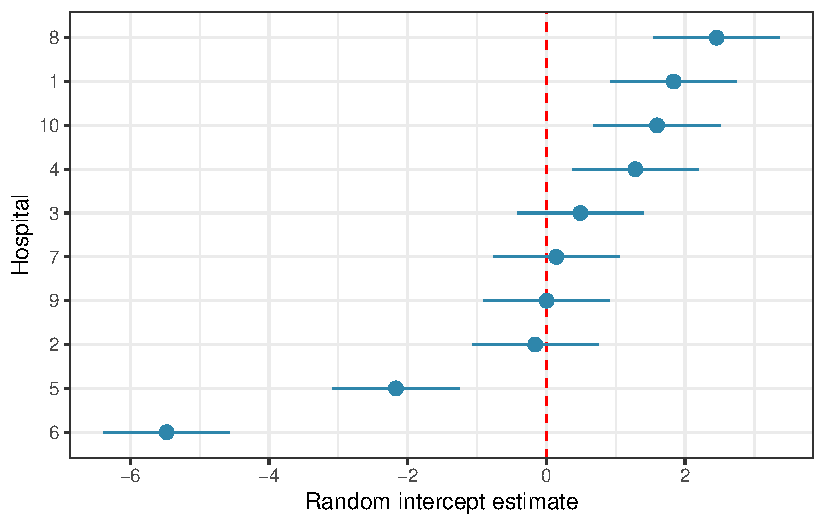
\includegraphics[width=0.9\textwidth,height=\textheight]{04b-mixed-effects_files/figure-pdf/fig-random-effects-extraction-1.pdf}

}

\caption{\label{fig-random-effects-extraction}Hospital random
intercepts. Estimated deviation of each hospital from the grand mean.}

\end{figure}%

The caterpillar plot shows the estimated random intercept for each
hospital with its 95\% uncertainty interval. Hospitals whose intervals
do not overlap zero are performing notably above or below average, after
accounting for the treatment effect.

\section{Degrees of Freedom and P-Values: The Kenward-Roger and
Satterthwaite
Debate}\label{degrees-of-freedom-and-p-values-the-kenward-roger-and-satterthwaite-debate}

\subsection{\texorpdfstring{Why \texttt{lme4} Does Not Give
P-Values}{Why lme4 Does Not Give P-Values}}\label{why-lme4-does-not-give-p-values}

Users fitting their first mixed model in R are often surprised to find
that \texttt{summary(fit\_ri)} produces \(t\) values for the fixed
effects but no p-values. This is not an oversight but a deliberate
design decision by the \texttt{lme4} authors, rooted in a genuine and
unresolved statistical problem.

In a standard linear model, the denominator degrees of freedom for each
\(F\) or \(t\) test are well defined and exact. In a mixed model, they
are not. The sampling distribution of the \(t\) statistic for a fixed
effect in a mixed model is approximately \(t\)-distributed, but the
degrees of freedom of that approximation depend on the covariance
structure of the random effects, the balance of the data, and the
specific parameter being tested and there is no universally agreed
formula for computing them. Using the wrong degrees of freedom can make
tests either too liberal or too conservative.

Two approximations are in common use, and both are implemented in the
\texttt{lmerTest} package \citep{Kuznetsova2017}:

\subsection{Satterthwaite's
Approximation}\label{satterthwaites-approximation}

Satterthwaite's method \citep{satterthwaite1946} estimates the effective
degrees of freedom for each fixed effect test by matching the moments of
the approximate \(t\) distribution to the variance components of the
model. It is computationally fast and works well for many standard
designs.

\begin{Shaded}
\begin{Highlighting}[]
\CommentTok{\# lmerTest automatically upgrades lmer() to provide p{-}values}
\NormalTok{fit\_ri\_test }\OtherTok{\textless{}{-}}\NormalTok{ lmerTest}\SpecialCharTok{::}\FunctionTok{lmer}\NormalTok{(outcome }\SpecialCharTok{\textasciitilde{}}\NormalTok{ treatment }\SpecialCharTok{+}\NormalTok{ (}\DecValTok{1} \SpecialCharTok{|}\NormalTok{ hospital), }\AttributeTok{data =}\NormalTok{ df\_lme, }\AttributeTok{REML =} \ConstantTok{TRUE}\NormalTok{)}
\FunctionTok{summary}\NormalTok{(fit\_ri\_test) }\CommentTok{\# now includes df and p{-}values}
\end{Highlighting}
\end{Shaded}

\begin{verbatim}
#> Linear mixed model fit by REML. t-tests use Satterthwaite's method [
#> lmerModLmerTest]
#> Formula: outcome ~ treatment + (1 | hospital)
#>    Data: df_lme
#> 
#> REML criterion at convergence: 897.6
#> 
#> Scaled residuals: 
#>     Min      1Q  Median      3Q     Max 
#> -2.8980 -0.6451  0.0198  0.5870  3.3917 
#> 
#> Random effects:
#>  Groups   Name        Variance Std.Dev.
#>  hospital (Intercept) 5.609    2.368   
#>  Residual             4.486    2.118   
#> Number of obs: 200, groups:  hospital, 10
#> 
#> Fixed effects:
#>                    Estimate Std. Error       df t value Pr(>|t|)    
#> (Intercept)         52.8446     0.7783   9.7048  67.895 2.54e-14 ***
#> treatmentTreatment   0.2663     0.2995 189.0000   0.889    0.375    
#> ---
#> Signif. codes:  0 '***' 0.001 '**' 0.01 '*' 0.05 '.' 0.1 ' ' 1
#> 
#> Correlation of Fixed Effects:
#>             (Intr)
#> trtmntTrtmn -0.192
\end{verbatim}

\begin{Shaded}
\begin{Highlighting}[]
\FunctionTok{anova}\NormalTok{(fit\_ri\_test) }\CommentTok{\# F tests with Satterthwaite df}
\end{Highlighting}
\end{Shaded}

\begin{verbatim}
#> Type III Analysis of Variance Table with Satterthwaite's method
#>           Sum Sq Mean Sq NumDF DenDF F value Pr(>F)
#> treatment 3.5466  3.5466     1   189  0.7905 0.3751
\end{verbatim}

The output now includes degrees of freedom and p-values for each fixed
effect, computed via Satterthwaite's approximation. The intercept is
highly significant (\(p < 0.001\)), but this is not a meaningful result
as it simply tests whether the grand mean recovery score differs from
zero, which is never a question of scientific interest. What matters is
the treatment coefficient: the new protocol does not produce a
significantly different recovery score from the control (\(p = 0.375\)),
consistent with the likelihood ratio test result from
Section~\ref{sec-reml-ml}.

The \texttt{anova()} call produces a Type III \(F\) test (see
Section~\ref{sec-type3}) for the treatment fixed effect using
Satterthwaite degrees of freedom. It reaches the same conclusion: no
significant difference between treatment groups. As a reminder, this
reflects the simulated data rather than a real clinical finding. The
true treatment effect in the simulation was small relative to the
within-hospital noise, and the study as simulated is underpowered to
detect it reliably.

\subsection{Kenward-Roger
Approximation}\label{kenward-roger-approximation}

The Kenward-Roger method \citep{Kenward1997} uses a more sophisticated
adjustment that also corrects the standard errors of the fixed effects
for small-sample bias in the variance component estimates. It is more
computationally demanding than Satterthwaite but is considered more
accurate, particularly with small numbers of groups or unbalanced
designs.

\begin{Shaded}
\begin{Highlighting}[]
\CommentTok{\# KR F test via lmerTest}
\FunctionTok{anova}\NormalTok{(fit\_ri\_test, }\AttributeTok{ddf =} \StringTok{"Kenward{-}Roger"}\NormalTok{)}
\end{Highlighting}
\end{Shaded}

\begin{verbatim}
#> Type III Analysis of Variance Table with Kenward-Roger's method
#>           Sum Sq Mean Sq NumDF DenDF F value Pr(>F)
#> treatment 3.5466  3.5466     1   189  0.7905 0.3751
\end{verbatim}

\begin{Shaded}
\begin{Highlighting}[]
\CommentTok{\# Or via pbkrtest directly}
\DocumentationTok{\#\# Kenward{-}Roger via lmerTest first}
\NormalTok{fit\_ri\_kr  }\OtherTok{\textless{}{-}}\NormalTok{ lmerTest}\SpecialCharTok{::}\FunctionTok{lmer}\NormalTok{(outcome }\SpecialCharTok{\textasciitilde{}}\NormalTok{ treatment }\SpecialCharTok{+}\NormalTok{ (}\DecValTok{1} \SpecialCharTok{|}\NormalTok{ hospital), }\AttributeTok{data =}\NormalTok{ df\_lme, }\AttributeTok{REML =} \ConstantTok{TRUE}\NormalTok{)}

\NormalTok{fit\_null\_kr }\OtherTok{\textless{}{-}}\NormalTok{ lmerTest}\SpecialCharTok{::}\FunctionTok{lmer}\NormalTok{(outcome }\SpecialCharTok{\textasciitilde{}} \DecValTok{1} \SpecialCharTok{+}\NormalTok{ (}\DecValTok{1} \SpecialCharTok{|}\NormalTok{ hospital), }\AttributeTok{data =}\NormalTok{ df\_lme, }\AttributeTok{REML =} \ConstantTok{TRUE}\NormalTok{)}

\CommentTok{\# Then test}
\NormalTok{pbkrtest}\SpecialCharTok{::}\FunctionTok{KRmodcomp}\NormalTok{(fit\_ri\_kr, fit\_null\_kr)}
\end{Highlighting}
\end{Shaded}

\begin{verbatim}
#> large : outcome ~ treatment + (1 | hospital)
#> small : outcome ~ 1 + (1 | hospital)
#>           stat      ndf      ddf F.scaling p.value
#> Ftest   0.7905   1.0000 189.0000         1  0.3751
\end{verbatim}

Both methods (\texttt{lmerTest} and \texttt{pbkrtest}) yield similar
results which are also similar to the previous one using Satterthwaite's
approximation. This reflects the simulated data and would not be the
case in a real case.

\subsection{Which Method to Use?}\label{which-method-to-use}

The practical guidance is straightforward:

\begin{longtable}[]{@{}
  >{\raggedright\arraybackslash}p{(\columnwidth - 2\tabcolsep) * \real{0.3667}}
  >{\raggedright\arraybackslash}p{(\columnwidth - 2\tabcolsep) * \real{0.6333}}@{}}
\toprule\noalign{}
\begin{minipage}[b]{\linewidth}\raggedright
Situation
\end{minipage} & \begin{minipage}[b]{\linewidth}\raggedright
Recommended method
\end{minipage} \\
\midrule\noalign{}
\endhead
\bottomrule\noalign{}
\endlastfoot
Large balanced dataset, many groups & Satterthwaite which is fast and
accurate \\
Small number of groups (\(< 20\)) & Kenward-Roger which is better
small-sample correction \\
Unbalanced design & Kenward-Roger which is more robust \\
Quick exploratory analysis & Satterthwaite which is an acceptable
approximation \\
Confirmatory clinical analysis & Kenward-Roger which is conservative and
defensible \\
\end{longtable}

Both methods give similar results with large, balanced datasets. The
differences matter most with small numbers of groups which is a common
situation in biology, where experiments often have 5-15 clusters. When
in doubt, use Kenward-Roger and note the method in your methods section.

\begin{tcolorbox}[enhanced jigsaw, title=\textcolor{quarto-callout-tip-color}{\faLightbulb}\hspace{0.5em}{Show me the maths!}, opacityback=0, bottomtitle=1mm, leftrule=.75mm, breakable, toprule=.15mm, colframe=quarto-callout-tip-color-frame, titlerule=0mm, rightrule=.15mm, toptitle=1mm, arc=.35mm, colback=white, left=2mm, colbacktitle=quarto-callout-tip-color!10!white, opacitybacktitle=0.6, coltitle=black, bottomrule=.15mm]

For the mathematical derivation of both the Satterthwaite and
Kenward-Roger degree of freedom approximations, see
\textbf{?@sec-df-approximations} in Appendix A.

\end{tcolorbox}

\section{Example: Patient Nested in Hospital Nested in
Region}\label{example-patient-nested-in-hospital-nested-in-region}

\subsection{The Study}\label{the-study-4}

A national health study investigates the effect of a new physiotherapy
protocol on functional recovery scores (0-100) in patients following
knee replacement surgery. Patients are recruited from 15 hospitals
distributed across 3 regions (Section~\ref{sec-physio}). Each hospital
contributes between 8 and 12 patients, assigned to either the standard
protocol (control) or the new physiotherapy protocol (treatment). The
hierarchical structure is:

\[\text{Region} \supset \text{Hospital} \supset \text{Patient}\]

Treatment is assigned at the patient level: individual patients within
the same hospital receive different protocols. This is important: it
means hospital and region are nuisance grouping factors that must be
accounted for, not treatment factors being tested.

\begin{Shaded}
\begin{Highlighting}[]
\FunctionTok{summary}\NormalTok{(physio)}
\end{Highlighting}
\end{Shaded}

\begin{verbatim}
#>     recovery         treatment     hospital  region 
#>  Min.   :39.19   Control  :78   H14    :12   R1:52  
#>  1st Qu.:57.59   Treatment:70   H23    :12   R2:45  
#>  Median :64.79                  H34    :12   R3:51  
#>  Mean   :64.38                  H12    :11          
#>  3rd Qu.:72.37                  H13    :11          
#>  Max.   :95.10                  H32    :11          
#>                                 (Other):79
\end{verbatim}

\begin{Shaded}
\begin{Highlighting}[]
\FunctionTok{cat}\NormalTok{(}
  \StringTok{"Total patients:"}\NormalTok{, }\FunctionTok{nrow}\NormalTok{(physio), }
  \StringTok{"}\SpecialCharTok{\textbackslash{}n}\StringTok{Patients per hospital:}\SpecialCharTok{\textbackslash{}n}\StringTok{"}\NormalTok{, }\FunctionTok{table}\NormalTok{(physio}\SpecialCharTok{$}\NormalTok{hospital)}
\NormalTok{  )}
\end{Highlighting}
\end{Shaded}

\begin{verbatim}
#> Total patients: 148 
#> Patients per hospital:
#>  9 11 11 12 9 8 9 12 8 8 10 11 9 12 9
\end{verbatim}

\subsection{Visualising the Nested
Structure}\label{visualising-the-nested-structure}

\begin{Shaded}
\begin{Highlighting}[]
\FunctionTok{library}\NormalTok{(ggplot2)}

\CommentTok{\# Hospital means}
\NormalTok{hosp\_means }\OtherTok{\textless{}{-}} \FunctionTok{aggregate}\NormalTok{(recovery }\SpecialCharTok{\textasciitilde{}}\NormalTok{ treatment }\SpecialCharTok{+}\NormalTok{ hospital }\SpecialCharTok{+}\NormalTok{ region, }\AttributeTok{data =}\NormalTok{ physio, }\AttributeTok{FUN =}\NormalTok{ mean)}

\FunctionTok{ggplot}\NormalTok{(physio, }\FunctionTok{aes}\NormalTok{(}\AttributeTok{x =}\NormalTok{ treatment, }\AttributeTok{y =}\NormalTok{ recovery, }\AttributeTok{colour =}\NormalTok{ hospital)) }\SpecialCharTok{+}
  \FunctionTok{geom\_jitter}\NormalTok{(}\AttributeTok{width =} \FloatTok{0.15}\NormalTok{, }\AttributeTok{alpha =} \FloatTok{0.4}\NormalTok{, }\AttributeTok{size =} \FloatTok{1.5}\NormalTok{) }\SpecialCharTok{+}
  \FunctionTok{geom\_point}\NormalTok{(}\AttributeTok{data =}\NormalTok{ hosp\_means, }\FunctionTok{aes}\NormalTok{(}\AttributeTok{y =}\NormalTok{ recovery), }\AttributeTok{size =} \DecValTok{4}\NormalTok{, }\AttributeTok{shape =} \DecValTok{18}\NormalTok{) }\SpecialCharTok{+}
  \FunctionTok{geom\_line}\NormalTok{(}\AttributeTok{data =}\NormalTok{ hosp\_means, }\FunctionTok{aes}\NormalTok{(}\AttributeTok{y =}\NormalTok{ recovery, }\AttributeTok{group =}\NormalTok{ hospital), }\AttributeTok{alpha =} \FloatTok{0.5}\NormalTok{) }\SpecialCharTok{+}
  \FunctionTok{facet\_wrap}\NormalTok{(}\SpecialCharTok{\textasciitilde{}}\NormalTok{ region, }\AttributeTok{labeller =}\NormalTok{ label\_both) }\SpecialCharTok{+}
  \FunctionTok{scale\_colour\_viridis\_d}\NormalTok{(}\AttributeTok{option =} \StringTok{"D"}\NormalTok{) }\SpecialCharTok{+}
  \FunctionTok{labs}\NormalTok{(}\AttributeTok{x =} \ConstantTok{NULL}\NormalTok{, }\AttributeTok{y =} \StringTok{"Recovery score"}\NormalTok{, }\AttributeTok{colour =} \StringTok{"Hospital"}\NormalTok{) }\SpecialCharTok{+}
  \FunctionTok{theme\_bw}\NormalTok{() }\SpecialCharTok{+}
  \FunctionTok{theme}\NormalTok{(}\AttributeTok{legend.position =} \StringTok{"bottom"}\NormalTok{)}
\end{Highlighting}
\end{Shaded}

\begin{figure}[H]

\centering{

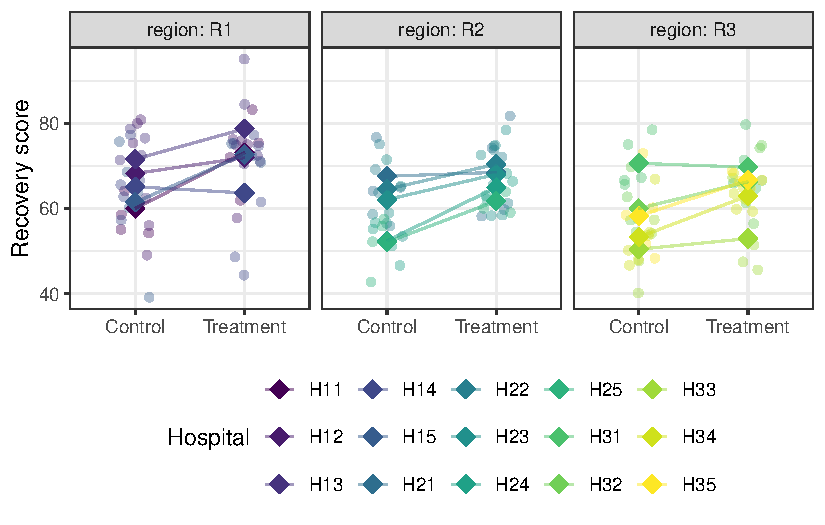
\includegraphics[width=0.9\textwidth,height=\textheight]{04b-mixed-effects_files/figure-pdf/fig-nested-plot-1.pdf}

}

\caption{\label{fig-nested-plot}Recovery scores by treatment group,
hospital, and region. Each panel is a region; within each panel, points
are coloured by hospital. The substantial variation in hospital means
within and across regions illustrates why the nested random effect
structure must be modelled explicitly.}

\end{figure}%

\subsection{Fitting the Three-Level Nested
Model}\label{fitting-the-three-level-nested-model}

\begin{Shaded}
\begin{Highlighting}[]
\FunctionTok{library}\NormalTok{(lme4)}
\FunctionTok{library}\NormalTok{(lmerTest)}
\end{Highlighting}
\end{Shaded}

\begin{verbatim}
#> 
#> Attaching package: 'lmerTest'
\end{verbatim}

\begin{verbatim}
#> The following object is masked from 'package:lme4':
#> 
#>     lmer
\end{verbatim}

\begin{verbatim}
#> The following object is masked from 'package:stats':
#> 
#>     step
\end{verbatim}

\begin{Shaded}
\begin{Highlighting}[]
\CommentTok{\# Three{-}level nested model:}
\CommentTok{\# hospital nested within region, both as random intercepts}
\NormalTok{fit\_nested }\OtherTok{\textless{}{-}} \FunctionTok{lmer}\NormalTok{(}
\NormalTok{  recovery }\SpecialCharTok{\textasciitilde{}}\NormalTok{ treatment }\SpecialCharTok{+}\NormalTok{ (}\DecValTok{1} \SpecialCharTok{|}\NormalTok{ region}\SpecialCharTok{/}\NormalTok{hospital),}
  \AttributeTok{data =}\NormalTok{ physio,}
  \AttributeTok{REML =} \ConstantTok{TRUE}
\NormalTok{)}

\FunctionTok{summary}\NormalTok{(fit\_nested)}
\end{Highlighting}
\end{Shaded}

\begin{verbatim}
#> Linear mixed model fit by REML. t-tests use Satterthwaite's method [
#> lmerModLmerTest]
#> Formula: recovery ~ treatment + (1 | region/hospital)
#>    Data: physio
#> 
#> REML criterion at convergence: 1053.2
#> 
#> Scaled residuals: 
#>      Min       1Q   Median       3Q      Max 
#> -3.07356 -0.62171  0.09592  0.59586  2.31967 
#> 
#> Random effects:
#>  Groups          Name        Variance Std.Dev.
#>  hospital:region (Intercept) 22.799   4.775   
#>  region          (Intercept)  8.732   2.955   
#>  Residual                    64.117   8.007   
#> Number of obs: 148, groups:  hospital:region, 15; region, 3
#> 
#> Fixed effects:
#>                    Estimate Std. Error      df t value Pr(>|t|)    
#> (Intercept)          61.329      2.294   2.351  26.740 0.000564 ***
#> treatmentTreatment    6.097      1.320 132.003   4.619 9.03e-06 ***
#> ---
#> Signif. codes:  0 '***' 0.001 '**' 0.01 '*' 0.05 '.' 0.1 ' ' 1
#> 
#> Correlation of Fixed Effects:
#>             (Intr)
#> trtmntTrtmn -0.272
\end{verbatim}

The \texttt{(1\ \textbar{}\ region/hospital)} notation specifies
hospital nested within region, equivalent to
\texttt{(1\ \textbar{}\ region)\ +\ (1\ \textbar{}\ region:hospital)}.
It produces three variance components: region-level variance
(\(\hat{\sigma}^2_{\text{region}}\)), hospital-within-region variance
(\(\hat{\sigma}^2_{\text{hospital}}\)), and residual patient-level
variance (\(\hat{\sigma}^2_\varepsilon\)).

The summary output reveals a clear and well-structured result across all
three sections.

\textbf{Random effects:} three variance components are estimated,
corresponding to the three levels of the hierarchy. The
hospital-within-region variance is
\(\hat{\sigma}^2_{\text{hospital}} = 22.80\) (SD = 4.78), the region
variance is \(\hat{\sigma}^2_{\text{region}} = 8.73\) (SD = 2.96), and
the residual patient-level variance is
\(\hat{\sigma}^2_\varepsilon = 64.12\) (SD = 8.01). The total variance
is therefore \(22.80 + 8.73 + 64.12 = 95.65\), of which the clustering
structure (hospital and region combined) accounts for
\((22.80 + 8.73) / 95.65 = 33\%\). This is a substantial ICC: one third
of the variation in recovery scores is attributable to which hospital
and region a patient belongs to, entirely independent of treatment. An
analysis that ignored this structure would dramatically underestimate
the uncertainty in the treatment effect estimate.

\textbf{Fixed effects:} the treatment coefficient is
\(\hat{\beta} = 6.10\) (SE = 1.32), with a Satterthwaite-approximated
\(t_{132} = 4.62\), \(p < 0.001\). Patients receiving the new
physiotherapy protocol recovered an estimated 6.1 points higher on the
recovery scale than control patients, after accounting for the hospital
and region clustering. This is a clinically meaningful and statistically
convincing result. Notice that the degrees of freedom for the treatment
test (132) are much larger than those for the intercept (2.35)
reflecting the fact that treatment was randomised at the patient level
(148 patients), while the intercept is estimated at the region level
(only 3 regions), where very little information is available. The
Satterthwaite approximation correctly propagates this distinction into
the inference.

The correlation between the intercept and treatment coefficient
estimates is \(-0.27\), indicating modest negative correlation:
hospitals with higher baseline recovery tend to show slightly smaller
treatment effects in the estimates, though this could be a property of
the estimation geometry rather than a substantive finding.

\textbf{Number of observations:} 148 patients are nested in 15
hospital-region combinations, which are in turn nested in 3 regions. The
modest number of regions (3) is the binding constraint on inference
about region-level effects and explains the very low degrees of freedom
(2.35) for the intercept test. With only 3 regions, the region-level
variance estimate (\(\hat{\sigma}^2_{\text {region}} = 8.73\)) should be
interpreted cautiously as it is based on very sparse information and
carries wide uncertainty.

\subsection{Diagnosing the Model}\label{diagnosing-the-model-1}

\begin{Shaded}
\begin{Highlighting}[]
\CommentTok{\# Residual plot}
\FunctionTok{plot}\NormalTok{(fit\_nested)}
\end{Highlighting}
\end{Shaded}

\begin{center}
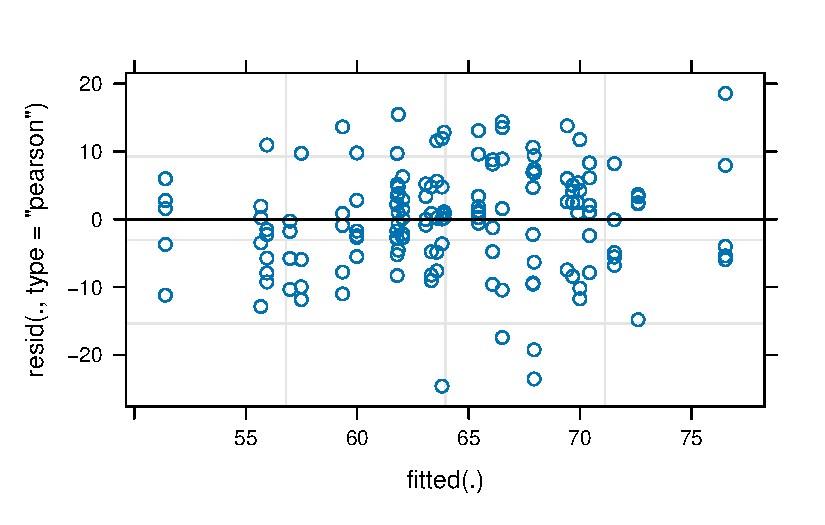
\includegraphics[width=0.9\textwidth,height=\textheight]{04b-mixed-effects_files/figure-pdf/nested-diagnostics-1.pdf}
\end{center}

\begin{Shaded}
\begin{Highlighting}[]
\CommentTok{\# Q{-}Q plot of residuals}
\FunctionTok{qqnorm}\NormalTok{(}\FunctionTok{resid}\NormalTok{(fit\_nested))}
\FunctionTok{qqline}\NormalTok{(}\FunctionTok{resid}\NormalTok{(fit\_nested), }\AttributeTok{col =} \StringTok{"red"}\NormalTok{)}
\end{Highlighting}
\end{Shaded}

\begin{center}
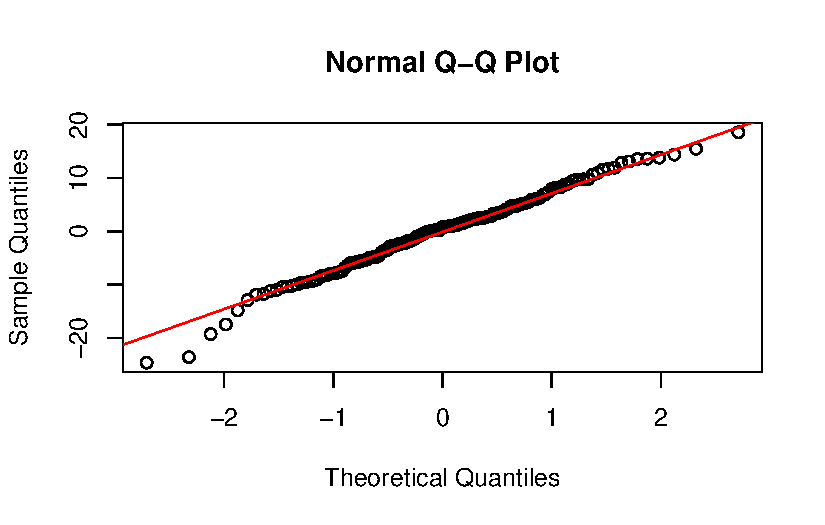
\includegraphics[width=0.9\textwidth,height=\textheight]{04b-mixed-effects_files/figure-pdf/nested-diagnostics-2.pdf}
\end{center}

\begin{Shaded}
\begin{Highlighting}[]
\CommentTok{\# Q{-}Q plot of random effects — should also be approximately normal}
\FunctionTok{qqnorm}\NormalTok{(}\FunctionTok{ranef}\NormalTok{(fit\_nested)}\SpecialCharTok{$}\NormalTok{hospital[, }\DecValTok{1}\NormalTok{], }\AttributeTok{main =} \StringTok{"Q{-}Q plot: hospital random effects"}\NormalTok{)}
\FunctionTok{qqline}\NormalTok{(}\FunctionTok{ranef}\NormalTok{(fit\_nested)}\SpecialCharTok{$}\NormalTok{hospital[, }\DecValTok{1}\NormalTok{], }\AttributeTok{col =} \StringTok{"red"}\NormalTok{)}
\end{Highlighting}
\end{Shaded}

\begin{center}
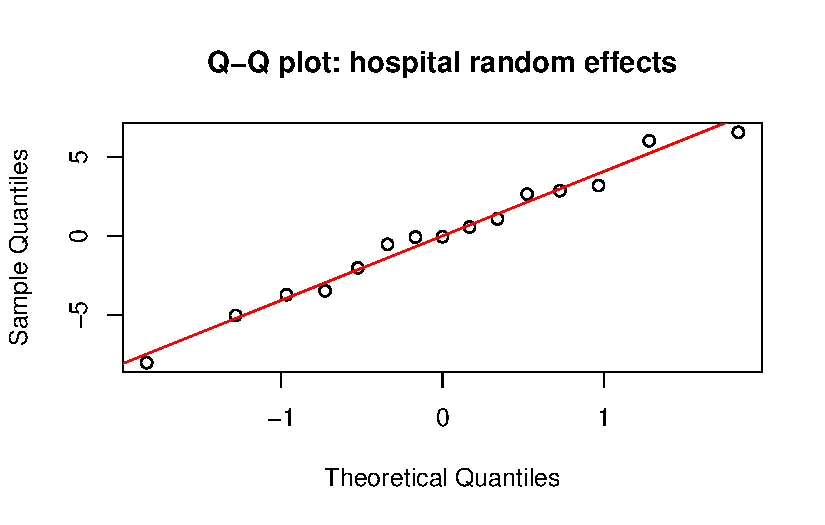
\includegraphics[width=0.9\textwidth,height=\textheight]{04b-mixed-effects_files/figure-pdf/nested-diagnostics-3.pdf}
\end{center}

A well-fitted mixed model should show approximately normal residuals
\emph{and} approximately normal random effects. The random effects Q-Q
plot is often overlooked: it tests the normality assumption on the
\(b_j\) directly, not just on the observation-level residuals.

\subsection{Testing the Fixed Effect}\label{testing-the-fixed-effect}

\begin{Shaded}
\begin{Highlighting}[]
\CommentTok{\# F test with Satterthwaite degrees of freedom}
\FunctionTok{anova}\NormalTok{(fit\_nested)}
\end{Highlighting}
\end{Shaded}

\begin{verbatim}
#> Type III Analysis of Variance Table with Satterthwaite's method
#>           Sum Sq Mean Sq NumDF DenDF F value    Pr(>F)    
#> treatment 1368.2  1368.2     1   132   21.34 9.028e-06 ***
#> ---
#> Signif. codes:  0 '***' 0.001 '**' 0.01 '*' 0.05 '.' 0.1 ' ' 1
\end{verbatim}

\begin{Shaded}
\begin{Highlighting}[]
\CommentTok{\# F test with Kenward{-}Roger degrees of freedom (preferred for small n)}
\FunctionTok{anova}\NormalTok{(fit\_nested, }\AttributeTok{ddf =} \StringTok{"Kenward{-}Roger"}\NormalTok{)}
\end{Highlighting}
\end{Shaded}

\begin{verbatim}
#> Type III Analysis of Variance Table with Kenward-Roger's method
#>           Sum Sq Mean Sq NumDF  DenDF F value    Pr(>F)    
#> treatment 1367.9  1367.9     1 132.15  21.334 9.044e-06 ***
#> ---
#> Signif. codes:  0 '***' 0.001 '**' 0.01 '*' 0.05 '.' 0.1 ' ' 1
\end{verbatim}

Both the Satterthwaite and Kenward-Roger F tests converge on the same
conclusion, and the agreement between them is reassuring. The
Satterthwaite test gives \(F_{1, 132.00} = 21.34\), \(p < 0.001\); the
Kenward-Roger test gives \(F_{1, 132.15} = 21.33\), \(p < 0.001\). The
two methods produce virtually identical results here because the dataset
is reasonably large at the patient level (148 observations) and the
design, while unbalanced, is not severely so. In a study with fewer
patients or more extreme imbalance across hospitals and regions, the two
methods would diverge more noticeably, and the Kenward-Roger result
would be the more trustworthy of the two.

The denominator degrees of freedom (132) confirm what the summary output
already showed: treatment is being tested at the patient level, where
replication is adequate. This is the correct behaviour as the new
protocol was randomised to individual patients, so the patient level is
the right level at which to evaluate it.

\begin{Shaded}
\begin{Highlighting}[]
\CommentTok{\# Effect size: marginal and conditional R{-}squared}
\CommentTok{\# install.packages("MuMIn") if needed}
\FunctionTok{library}\NormalTok{(MuMIn)}
\FunctionTok{r.squaredGLMM}\NormalTok{(fit\_nested)}
\end{Highlighting}
\end{Shaded}

\begin{verbatim}
#>             R2m      R2c
#> [1,] 0.08885778 0.389217
\end{verbatim}

\texttt{r.squaredGLMM()} returns two R² values for mixed models:

\begin{itemize}
\tightlist
\item
  \textbf{Marginal R²} (\(R^2_m\)): the proportion of variance explained
  by the fixed effects alone, here, the treatment effect.
\item
  \textbf{Conditional R²} (\(R^2_c\)): the proportion of variance
  explained by both fixed and random effects together which is the full
  model.
\end{itemize}

The difference between them (\(R^2_c - R^2_m\)) reflects how much of the
total variation is attributable to the random effects, in this example
it correspond to the hospital and region clustering structure.

In the example, the R² values from \texttt{r.squaredGLMM()} decompose
the explained variance informatively. The marginal R² is
\(R^2_m = 0.089\), meaning the treatment fixed effect alone explains
approximately 9\% of the total variation in recovery scores. The
conditional R² is \(R^2_c = 0.389\), meaning the full model explains
39\% of total variation. The difference, \(R^2_c - R^2_m = 0.300\), is
the contribution of the hospital and region clustering structure: 30\%
of total variation is attributable to which hospital and region a
patient belongs to, over and above the treatment effect. This is a
striking reminder of why the random effects cannot be ignored: the
clustering explains more than three times as much variation as the
treatment itself, and failing to account for it would have produced
severely misleading standard errors and p-values for the treatment
comparison.

\subsection{Comparing Nested Models}\label{comparing-nested-models}

To formally test whether the random effects are necessary, whether
hospital and region clustering is real, compare models with and without
the random effects using likelihood ratio tests:

\begin{Shaded}
\begin{Highlighting}[]
\CommentTok{\# Fit models with ML for comparison of fixed effects}
\NormalTok{fit\_full }\OtherTok{\textless{}{-}}\NormalTok{ lme4}\SpecialCharTok{::}\FunctionTok{lmer}\NormalTok{(recovery }\SpecialCharTok{\textasciitilde{}}\NormalTok{ treatment }\SpecialCharTok{+}\NormalTok{ (}\DecValTok{1} \SpecialCharTok{|}\NormalTok{ region}\SpecialCharTok{/}\NormalTok{hospital),}
                       \AttributeTok{data =}\NormalTok{ physio, }\AttributeTok{REML =} \ConstantTok{FALSE}\NormalTok{)}
\NormalTok{fit\_no\_h }\OtherTok{\textless{}{-}}\NormalTok{ lme4}\SpecialCharTok{::}\FunctionTok{lmer}\NormalTok{(recovery }\SpecialCharTok{\textasciitilde{}}\NormalTok{ treatment }\SpecialCharTok{+}\NormalTok{ (}\DecValTok{1} \SpecialCharTok{|}\NormalTok{ region),}
                       \AttributeTok{data =}\NormalTok{ physio, }\AttributeTok{REML =} \ConstantTok{FALSE}\NormalTok{)}

\CommentTok{\# Is hospital{-}within{-}region variance significant?}
\CommentTok{\# Compare model with and without hospital{-}level random effect}
\FunctionTok{anova}\NormalTok{(fit\_no\_h, fit\_full)}
\end{Highlighting}
\end{Shaded}

\begin{verbatim}
#> Data: physio
#> Models:
#> fit_no_h: recovery ~ treatment + (1 | region)
#> fit_full: recovery ~ treatment + (1 | region/hospital)
#>          npar    AIC    BIC  logLik -2*log(L) Chisq Df Pr(>Chisq)    
#> fit_no_h    4 1085.1 1097.1 -538.56    1077.1                        
#> fit_full    5 1068.8 1083.8 -529.40    1058.8 18.33  1  1.858e-05 ***
#> ---
#> Signif. codes:  0 '***' 0.001 '**' 0.01 '*' 0.05 '.' 0.1 ' ' 1
\end{verbatim}

\begin{Shaded}
\begin{Highlighting}[]
\CommentTok{\# Is region variance significant?}
\CommentTok{\# Compare model with and without region{-}level random effect}
\NormalTok{fit\_no\_r }\OtherTok{\textless{}{-}}\NormalTok{ lme4}\SpecialCharTok{::}\FunctionTok{lmer}\NormalTok{(recovery }\SpecialCharTok{\textasciitilde{}}\NormalTok{ treatment }\SpecialCharTok{+}\NormalTok{ (}\DecValTok{1} \SpecialCharTok{|}\NormalTok{ hospital),}
                       \AttributeTok{data =}\NormalTok{ physio, }\AttributeTok{REML =} \ConstantTok{FALSE}\NormalTok{)}
\FunctionTok{anova}\NormalTok{(fit\_no\_r, fit\_full)}
\end{Highlighting}
\end{Shaded}

\begin{verbatim}
#> Data: physio
#> Models:
#> fit_no_r: recovery ~ treatment + (1 | hospital)
#> fit_full: recovery ~ treatment + (1 | region/hospital)
#>          npar    AIC    BIC  logLik -2*log(L)  Chisq Df Pr(>Chisq)
#> fit_no_r    4 1067.1 1079.1 -529.57    1059.1                     
#> fit_full    5 1068.8 1083.8 -529.40    1058.8 0.3455  1     0.5567
\end{verbatim}

\begin{Shaded}
\begin{Highlighting}[]
\CommentTok{\# Alternative: ranova() tests each random effect term directly}
\CommentTok{\# without needing to refit models manually}
\NormalTok{lmerTest}\SpecialCharTok{::}\FunctionTok{ranova}\NormalTok{(}
\NormalTok{  lmerTest}\SpecialCharTok{::}\FunctionTok{lmer}\NormalTok{(recovery }\SpecialCharTok{\textasciitilde{}}\NormalTok{ treatment }\SpecialCharTok{+}\NormalTok{ (}\DecValTok{1} \SpecialCharTok{|}\NormalTok{ region}\SpecialCharTok{/}\NormalTok{hospital),}
                 \AttributeTok{data =}\NormalTok{ physio, }\AttributeTok{REML =} \ConstantTok{TRUE}\NormalTok{)}
\NormalTok{)}
\end{Highlighting}
\end{Shaded}

\begin{verbatim}
#> ANOVA-like table for random-effects: Single term deletions
#> 
#> Model:
#> recovery ~ treatment + (1 | hospital:region) + (1 | region)
#>                       npar  logLik    AIC     LRT Df Pr(>Chisq)    
#> <none>                   5 -526.60 1063.2                          
#> (1 | hospital:region)    4 -535.64 1079.3 18.0884  1  2.109e-05 ***
#> (1 | region)             4 -527.04 1062.1  0.8802  1     0.3481    
#> ---
#> Signif. codes:  0 '***' 0.001 '**' 0.01 '*' 0.05 '.' 0.1 ' ' 1
\end{verbatim}

The model comparison results tell a nuanced but clear story about the
necessity of each level of the random effects structure.

The hospital-within-region random effect is strongly supported by the
data. Removing it significantly worsens the model fit
(\(\chi^2_1 = 18.33\), \(p < 0.001\)), and the AIC drops from 1085.1 to
1068.8 when hospital-level clustering is included. The 18 unit
improvement in log-likelihood is substantial, the 15 hospitals differ
from each other in their baseline recovery levels in ways that cannot be
explained by region alone, and ignoring this hospital-level clustering
would produce incorrect standard errors for the treatment comparison.

The region random effect, however, tells a different story. Removing it
does not significantly worsen the fit (\(\chi^2_1 = 0.35\),
\(p = 0.557\)), and the AIC is actually slightly lower without it
(1067.1 vs 1068.8). The \texttt{ranova()} output confirms this: the
hospital-within-region term is highly significant (\(\chi^2_1 = 18.09\),
\(p < 0.001\)) while the region term is not (\(\chi^2_1 = 0.88\),
\(p = 0.348\)). With only 3 regions in the study, the region-level
variance (\(\hat{\sigma}^2_{\text{region}} = 8.73\)) is estimated from
very sparse information and the likelihood ratio test has almost no
power to detect it even if it is real. This is a common situation in
hierarchical biological studies: the highest level of the hierarchy is
almost always the most sparsely replicated, and non-significant tests
for top-level random effects should be interpreted as reflecting limited
power rather than genuine absence of region-level variation. In this
case, retaining the region random effect is the scientifically
conservative and appropriate choice. Indeed, the three regions were
sampled from a larger population of regions and their variation should
be accounted for regardless of the test result.

\subsection{Reporting the Result}\label{reporting-the-result-1}

\begin{Shaded}
\begin{Highlighting}[]
\CommentTok{\# Final model refitted with REML for reporting}
\NormalTok{fit\_final }\OtherTok{\textless{}{-}}\NormalTok{ lmerTest}\SpecialCharTok{::}\FunctionTok{lmer}\NormalTok{(}
\NormalTok{  recovery }\SpecialCharTok{\textasciitilde{}}\NormalTok{ treatment }\SpecialCharTok{+}\NormalTok{ (}\DecValTok{1} \SpecialCharTok{|}\NormalTok{ region}\SpecialCharTok{/}\NormalTok{hospital),}
  \AttributeTok{data =}\NormalTok{ physio, }\AttributeTok{REML =} \ConstantTok{TRUE}
\NormalTok{)}
\FunctionTok{summary}\NormalTok{(fit\_final)}
\end{Highlighting}
\end{Shaded}

\begin{verbatim}
#> Linear mixed model fit by REML. t-tests use Satterthwaite's method [
#> lmerModLmerTest]
#> Formula: recovery ~ treatment + (1 | region/hospital)
#>    Data: physio
#> 
#> REML criterion at convergence: 1053.2
#> 
#> Scaled residuals: 
#>      Min       1Q   Median       3Q      Max 
#> -3.07356 -0.62171  0.09592  0.59586  2.31967 
#> 
#> Random effects:
#>  Groups          Name        Variance Std.Dev.
#>  hospital:region (Intercept) 22.799   4.775   
#>  region          (Intercept)  8.732   2.955   
#>  Residual                    64.117   8.007   
#> Number of obs: 148, groups:  hospital:region, 15; region, 3
#> 
#> Fixed effects:
#>                    Estimate Std. Error      df t value Pr(>|t|)    
#> (Intercept)          61.329      2.294   2.351  26.740 0.000564 ***
#> treatmentTreatment    6.097      1.320 132.003   4.619 9.03e-06 ***
#> ---
#> Signif. codes:  0 '***' 0.001 '**' 0.01 '*' 0.05 '.' 0.1 ' ' 1
#> 
#> Correlation of Fixed Effects:
#>             (Intr)
#> trtmntTrtmn -0.272
\end{verbatim}

\begin{Shaded}
\begin{Highlighting}[]
\FunctionTok{anova}\NormalTok{(fit\_final, }\AttributeTok{ddf =} \StringTok{"Kenward{-}Roger"}\NormalTok{)}
\end{Highlighting}
\end{Shaded}

\begin{verbatim}
#> Type III Analysis of Variance Table with Kenward-Roger's method
#>           Sum Sq Mean Sq NumDF  DenDF F value    Pr(>F)    
#> treatment 1367.9  1367.9     1 132.15  21.334 9.044e-06 ***
#> ---
#> Signif. codes:  0 '***' 0.001 '**' 0.01 '*' 0.05 '.' 0.1 ' ' 1
\end{verbatim}

\begin{Shaded}
\begin{Highlighting}[]
\FunctionTok{r.squaredGLMM}\NormalTok{(fit\_final)}
\end{Highlighting}
\end{Shaded}

\begin{verbatim}
#>             R2m      R2c
#> [1,] 0.08885778 0.389217
\end{verbatim}

A complete report of the three-level nested analysis:

\begin{quote}
Recovery scores following knee replacement surgery were analysed using a
three-level linear mixed-effects model with treatment (control vs new
physiotherapy protocol) as a fixed effect and random intercepts for
hospital nested within region, fitted by REML using \texttt{lme4}
version 1.x \citep{Bates2015}. Degrees of freedom for fixed effect tests
were approximated using the Kenward-Roger method \citep{Kenward1997} via
\texttt{lmerTest} \citep{Kuznetsova2017}.

The new physiotherapy protocol was associated with significantly higher
recovery scores than the standard protocol (\(\beta = 6.10\),
\(SE = 1.32\), \(F_{1, 132.15} = 21.33\), \(p < 0.001\)). The marginal
\(R^2\) was 0.089, indicating that the treatment effect alone explained
9\% of total variance in recovery scores. The conditional \(R^2\) was
0.389, with the random effects accounting for an additional 30\% of
total variance, confirming that the hierarchical structure of the data
(patients clustered within hospitals, hospitals clustered within
regions) was a substantial source of variation that required explicit
modelling.

Likelihood ratio tests confirmed significant variance at the
hospital-within-region level (\(\chi^2_1 = 18.33\), \(p < 0.001\)), with
estimated hospital-level standard deviation of 4.78 recovery points.
Region-level variance did not reach significance (\(\chi^2_1 = 0.35\),
\(p = 0.557\)), though with only three regions the test had limited
power, and the region random effect was retained in the model on
scientific grounds. Residual patient-level standard deviation was 8.01
recovery points.
\end{quote}

\section{Repeated Measures as a Mixed Model}\label{sec-repeat-mixed}

\subsection{The Connection to Chapter
6}\label{the-connection-to-chapter-6}

Chapter \textbf{?@sec-repeated} analysed repeated measures data using
\texttt{aov()} with an \texttt{Error()} term which is the classical
approach that has been standard in biology for decades. That approach
works well for balanced designs with complete data, but it has three
important limitations that become apparent in practice: it cannot handle
missing observations, it assumes a specific covariance structure
(compound symmetry, closely related to sphericity), and it becomes
unwieldy with more than two levels of nesting.

Mixed-effects models handle all three limitations naturally. And because
the repeated measures model is already a mixed model in disguise,
subjects are a random effect, time is a fixed effect, the transition
requires no new conceptual machinery. It is simply a matter of fitting
the same model with \texttt{lmer()} instead of \texttt{aov()}.

\subsection{Refitting the Clinical
Example}\label{refitting-the-clinical-example}

We return to the cardiac rehabilitation trial from Chapter 6: 40
patients (20 control, 20 intervention) measured at weeks 0, 4, 8, and 12
(Section~\ref{sec-cardiac-recovery}). We first refit the classical
repeated measures ANOVA, then refit the same model as a mixed-effects
model, and compare the results directly.

\begin{Shaded}
\begin{Highlighting}[]
\FunctionTok{library}\NormalTok{(lme4)}
\FunctionTok{library}\NormalTok{(lmerTest)}

\CommentTok{\# Classical repeated measures ANOVA from Chapter 6}
\NormalTok{fit\_rm\_classical }\OtherTok{\textless{}{-}} \FunctionTok{aov}\NormalTok{(}
\NormalTok{  hr }\SpecialCharTok{\textasciitilde{}}\NormalTok{ group }\SpecialCharTok{*}\NormalTok{ time }\SpecialCharTok{+} \FunctionTok{Error}\NormalTok{(subject}\SpecialCharTok{/}\NormalTok{time),}
  \AttributeTok{data =}\NormalTok{ cardiac\_recovery}
\NormalTok{)}
\FunctionTok{summary}\NormalTok{(fit\_rm\_classical)}
\end{Highlighting}
\end{Shaded}

\begin{verbatim}
#> 
#> Error: subject
#>           Df Sum Sq Mean Sq F value   Pr(>F)    
#> group      1  883.3   883.3   19.09 9.29e-05 ***
#> Residuals 38 1757.9    46.3                     
#> ---
#> Signif. codes:  0 '***' 0.001 '**' 0.01 '*' 0.05 '.' 0.1 ' ' 1
#> 
#> Error: subject:time
#>             Df Sum Sq Mean Sq F value   Pr(>F)    
#> time         3 1811.6   603.9   66.98  < 2e-16 ***
#> group:time   3  598.8   199.6   22.14 2.28e-11 ***
#> Residuals  114 1027.7     9.0                     
#> ---
#> Signif. codes:  0 '***' 0.001 '**' 0.01 '*' 0.05 '.' 0.1 ' ' 1
\end{verbatim}

\begin{Shaded}
\begin{Highlighting}[]
\CommentTok{\# The same model as a linear mixed{-}effects model}
\CommentTok{\# subject is the random effect; group and time are fixed}
\NormalTok{fit\_rm\_mixed }\OtherTok{\textless{}{-}}\NormalTok{ lmerTest}\SpecialCharTok{::}\FunctionTok{lmer}\NormalTok{(}
\NormalTok{  hr }\SpecialCharTok{\textasciitilde{}}\NormalTok{ group }\SpecialCharTok{*}\NormalTok{ time }\SpecialCharTok{+}\NormalTok{ (}\DecValTok{1} \SpecialCharTok{|}\NormalTok{ subject),}
  \AttributeTok{data =}\NormalTok{ cardiac\_recovery,}
  \AttributeTok{REML =} \ConstantTok{TRUE}
\NormalTok{)}
\FunctionTok{summary}\NormalTok{(fit\_rm\_mixed)}
\end{Highlighting}
\end{Shaded}

\begin{verbatim}
#> Linear mixed model fit by REML. t-tests use Satterthwaite's method [
#> lmerModLmerTest]
#> Formula: hr ~ group * time + (1 | subject)
#>    Data: cardiac_recovery
#> 
#> REML criterion at convergence: 851.7
#> 
#> Scaled residuals: 
#>      Min       1Q   Median       3Q      Max 
#> -3.00986 -0.60094  0.06222  0.49595  2.85033 
#> 
#> Random effects:
#>  Groups   Name        Variance Std.Dev.
#>  subject  (Intercept) 9.311    3.051   
#>  Residual             9.015    3.002   
#> Number of obs: 160, groups:  subject, 40
#> 
#> Fixed effects:
#>                          Estimate Std. Error       df t value Pr(>|t|)    
#> (Intercept)               80.9464     0.9572  85.6600  84.562  < 2e-16 ***
#> groupIntervention          0.2611     1.3537  85.6600   0.193  0.84752    
#> time4                     -2.1052     0.9495 114.0000  -2.217  0.02859 *  
#> time8                     -3.0179     0.9495 114.0000  -3.179  0.00191 ** 
#> time12                    -3.9646     0.9495 114.0000  -4.176 5.84e-05 ***
#> groupIntervention:time4   -2.5790     1.3428 114.0000  -1.921  0.05727 .  
#> groupIntervention:time8   -7.4799     1.3428 114.0000  -5.571 1.72e-07 ***
#> groupIntervention:time12  -9.7825     1.3428 114.0000  -7.285 4.48e-11 ***
#> ---
#> Signif. codes:  0 '***' 0.001 '**' 0.01 '*' 0.05 '.' 0.1 ' ' 1
#> 
#> Correlation of Fixed Effects:
#>             (Intr) grpInt time4  time8  time12 grpI:4 grpI:8
#> grpIntrvntn -0.707                                          
#> time4       -0.496  0.351                                   
#> time8       -0.496  0.351  0.500                            
#> time12      -0.496  0.351  0.500  0.500                     
#> grpIntrvn:4  0.351 -0.496 -0.707 -0.354 -0.354              
#> grpIntrvn:8  0.351 -0.496 -0.354 -0.707 -0.354  0.500       
#> grpIntrv:12  0.351 -0.496 -0.354 -0.354 -0.707  0.500  0.500
\end{verbatim}

\begin{Shaded}
\begin{Highlighting}[]
\FunctionTok{anova}\NormalTok{(fit\_rm\_mixed, }\AttributeTok{ddf =} \StringTok{"Satterthwaite"}\NormalTok{)}
\end{Highlighting}
\end{Shaded}

\begin{verbatim}
#> Type III Analysis of Variance Table with Satterthwaite's method
#>             Sum Sq Mean Sq NumDF DenDF F value    Pr(>F)    
#> group       172.14  172.14     1    38  19.095 9.292e-05 ***
#> time       1811.55  603.85     3   114  66.983 < 2.2e-16 ***
#> group:time  598.77  199.59     3   114  22.140 2.280e-11 ***
#> ---
#> Signif. codes:  0 '***' 0.001 '**' 0.01 '*' 0.05 '.' 0.1 ' ' 1
\end{verbatim}

With complete, balanced data the two approaches give the same \(F\)
statistics, the same degrees of freedom, and the same p-values for every
effect. This equivalence is not a coincidence: the \texttt{Error()}
specification in \texttt{aov()} and the
\texttt{(1\ \textbar{}\ subject)} random intercept in \texttt{lmer()}
are two syntaxes for the same statistical model. The subject random
intercept absorbs the stable between-patient differences in heart rate,
leaving the within-subject residual as the error term against which the
time and group-by-time effects are tested which is exactly what the
\texttt{Error(subject/time)} stratum does in the classical output.

\subsection{Where the Two Approaches
Diverge}\label{where-the-two-approaches-diverge}

The equivalence breaks down in three practically important situations.

\textbf{Missing data.} \texttt{aov()} with \texttt{Error()} performs
listwise deletion: any subject with a missing observation at any time
point is excluded entirely from the analysis. \texttt{lmer()} uses REML
or ML estimation, which retains all available observations under the
missing-at-random assumption. In a 12-week clinical trial where some
patients miss appointments, this difference can be substantial.

\begin{Shaded}
\begin{Highlighting}[]
\CommentTok{\# Introduce missing data: remove 5 random observations}
\FunctionTok{set.seed}\NormalTok{(}\DecValTok{42}\NormalTok{)}
\NormalTok{df\_missing }\OtherTok{\textless{}{-}}\NormalTok{ cardiac\_recovery}
\NormalTok{missing\_idx }\OtherTok{\textless{}{-}} \FunctionTok{sample}\NormalTok{(}\FunctionTok{nrow}\NormalTok{(df\_missing), }\DecValTok{5}\NormalTok{)}
\NormalTok{df\_missing}\SpecialCharTok{$}\NormalTok{hr[missing\_idx] }\OtherTok{\textless{}{-}} \ConstantTok{NA}

\CommentTok{\# Classical approach: drops entire subjects with any missing value}
\NormalTok{fit\_classical\_miss }\OtherTok{\textless{}{-}} \FunctionTok{aov}\NormalTok{(}
\NormalTok{  hr }\SpecialCharTok{\textasciitilde{}}\NormalTok{ group }\SpecialCharTok{*}\NormalTok{ time }\SpecialCharTok{+} \FunctionTok{Error}\NormalTok{(subject}\SpecialCharTok{/}\NormalTok{time),}
  \AttributeTok{data =}\NormalTok{ df\_missing}
\NormalTok{)}
\FunctionTok{cat}\NormalTok{(}\StringTok{"Classical ANOVA, subjects retained:"}\NormalTok{,}
    \FunctionTok{length}\NormalTok{(}\FunctionTok{unique}\NormalTok{(}
\NormalTok{      df\_missing}\SpecialCharTok{$}\NormalTok{subject[}\FunctionTok{complete.cases}\NormalTok{(df\_missing)]}
\NormalTok{    )), }\StringTok{"}\SpecialCharTok{\textbackslash{}n}\StringTok{"}\NormalTok{)}
\end{Highlighting}
\end{Shaded}

\begin{verbatim}
#> Classical ANOVA, subjects retained: 40
\end{verbatim}

\begin{Shaded}
\begin{Highlighting}[]
\CommentTok{\# Mixed model: retains all subjects, uses all available observations}
\NormalTok{fit\_mixed\_miss }\OtherTok{\textless{}{-}}\NormalTok{ lmerTest}\SpecialCharTok{::}\FunctionTok{lmer}\NormalTok{(}
\NormalTok{  hr }\SpecialCharTok{\textasciitilde{}}\NormalTok{ group }\SpecialCharTok{*}\NormalTok{ time }\SpecialCharTok{+}\NormalTok{ (}\DecValTok{1} \SpecialCharTok{|}\NormalTok{ subject),}
  \AttributeTok{data =}\NormalTok{ df\_missing,}
  \AttributeTok{REML =} \ConstantTok{TRUE}\NormalTok{,}
  \AttributeTok{na.action =}\NormalTok{ na.omit}
\NormalTok{)}
\FunctionTok{cat}\NormalTok{(}\StringTok{"Mixed model, observations used:"}\NormalTok{, }\FunctionTok{nobs}\NormalTok{(fit\_mixed\_miss), }\StringTok{"}\SpecialCharTok{\textbackslash{}n}\StringTok{"}\NormalTok{)}
\end{Highlighting}
\end{Shaded}

\begin{verbatim}
#> Mixed model, observations used: 155
\end{verbatim}

\textbf{Unequal time spacing.} \texttt{aov()} treats the time factor as
a nominal categorical variable making the spacing between time points is
irrelevant. \texttt{lmer()} can model time as a continuous variable,
allowing the trajectory to be estimated as a smooth function (linear,
quadratic, or piecewise) rather than a step function. This is more
parsimonious and often more biologically sensible.

\begin{Shaded}
\begin{Highlighting}[]
\CommentTok{\# Group means per time point}
\NormalTok{summ }\OtherTok{\textless{}{-}} \FunctionTok{aggregate}\NormalTok{(hr }\SpecialCharTok{\textasciitilde{}}\NormalTok{ group }\SpecialCharTok{+}\NormalTok{ time, }\AttributeTok{data =}\NormalTok{ cardiac\_recovery, }\AttributeTok{FUN =}\NormalTok{ mean)}
\NormalTok{summ}\SpecialCharTok{$}\NormalTok{time\_num }\OtherTok{\textless{}{-}} \FunctionTok{as.numeric}\NormalTok{(}\FunctionTok{as.character}\NormalTok{(summ}\SpecialCharTok{$}\NormalTok{time))}

\NormalTok{cardiac\_recovery}\SpecialCharTok{$}\NormalTok{time\_num }\OtherTok{\textless{}{-}} \FunctionTok{as.numeric}\NormalTok{(}\FunctionTok{as.character}\NormalTok{(cardiac\_recovery}\SpecialCharTok{$}\NormalTok{time))}

\CommentTok{\# Model time as continuous, estimates a linear trajectory}
\CommentTok{\# rather than separate means at each time point}
\NormalTok{fit\_rm\_linear }\OtherTok{\textless{}{-}}\NormalTok{ lmerTest}\SpecialCharTok{::}\FunctionTok{lmer}\NormalTok{(}
\NormalTok{  hr }\SpecialCharTok{\textasciitilde{}}\NormalTok{ group }\SpecialCharTok{*}\NormalTok{ time\_num }\SpecialCharTok{+}\NormalTok{ (}\DecValTok{1} \SpecialCharTok{|}\NormalTok{ subject),}
  \AttributeTok{data =}\NormalTok{ cardiac\_recovery,}
  \AttributeTok{REML =} \ConstantTok{TRUE}
\NormalTok{)}

\FunctionTok{anova}\NormalTok{(fit\_rm\_linear, }\AttributeTok{ddf =} \StringTok{"Kenward{-}Roger"}\NormalTok{)}
\end{Highlighting}
\end{Shaded}

\begin{verbatim}
#> Type III Analysis of Variance Table with Kenward-Roger's method
#>                 Sum Sq Mean Sq NumDF   DenDF  F value    Pr(>F)    
#> group             1.10    1.10     1  66.583   0.1229     0.727    
#> time_num       1791.70 1791.70     1 118.000 199.4800 < 2.2e-16 ***
#> group:time_num  586.47  586.47     1 118.000  65.2953 6.281e-13 ***
#> ---
#> Signif. codes:  0 '***' 0.001 '**' 0.01 '*' 0.05 '.' 0.1 ' ' 1
\end{verbatim}

\begin{Shaded}
\begin{Highlighting}[]
\CommentTok{\# Model time as continuous with random slope}
\CommentTok{\# allows each patient to have their own rate of change}
\NormalTok{fit\_rm\_rslope }\OtherTok{\textless{}{-}}\NormalTok{ lmerTest}\SpecialCharTok{::}\FunctionTok{lmer}\NormalTok{(}
\NormalTok{  hr }\SpecialCharTok{\textasciitilde{}}\NormalTok{ group }\SpecialCharTok{*}\NormalTok{ time\_num }\SpecialCharTok{+}\NormalTok{ (time\_num }\SpecialCharTok{|}\NormalTok{ subject),}
  \AttributeTok{data =}\NormalTok{ cardiac\_recovery,}
  \AttributeTok{REML =} \ConstantTok{TRUE}
\NormalTok{)}
\FunctionTok{anova}\NormalTok{(fit\_rm\_rslope, }\AttributeTok{ddf =} \StringTok{"Kenward{-}Roger"}\NormalTok{)}
\end{Highlighting}
\end{Shaded}

\begin{verbatim}
#> Type III Analysis of Variance Table with Kenward-Roger's method
#>                Sum Sq Mean Sq NumDF DenDF  F value    Pr(>F)    
#> group            0.91    0.91     1    38   0.1451    0.7054    
#> time_num       762.91  762.91     1    38 121.8251 2.049e-13 ***
#> group:time_num 249.72  249.72     1    38  39.8768 2.108e-07 ***
#> ---
#> Signif. codes:  0 '***' 0.001 '**' 0.01 '*' 0.05 '.' 0.1 ' ' 1
\end{verbatim}

\begin{Shaded}
\begin{Highlighting}[]
\CommentTok{\# Does the random slope improve fit?}
\CommentTok{\# Use ML for model comparison}
\NormalTok{rm\_linear\_ml }\OtherTok{\textless{}{-}}\NormalTok{ lme4}\SpecialCharTok{::}\FunctionTok{lmer}\NormalTok{(}
\NormalTok{  hr }\SpecialCharTok{\textasciitilde{}}\NormalTok{ group }\SpecialCharTok{*}\NormalTok{ time\_num }\SpecialCharTok{+}\NormalTok{ (}\DecValTok{1} \SpecialCharTok{|}\NormalTok{ subject),}
  \AttributeTok{data =}\NormalTok{ cardiac\_recovery, }\AttributeTok{REML =} \ConstantTok{FALSE}
\NormalTok{  )}
\NormalTok{rm\_rslope\_ml }\OtherTok{\textless{}{-}}\NormalTok{ lme4}\SpecialCharTok{::}\FunctionTok{lmer}\NormalTok{(}
\NormalTok{  hr }\SpecialCharTok{\textasciitilde{}}\NormalTok{ group }\SpecialCharTok{*}\NormalTok{ time\_num }\SpecialCharTok{+}\NormalTok{ (time\_num }\SpecialCharTok{|}\NormalTok{ subject), }
  \AttributeTok{data =}\NormalTok{ cardiac\_recovery, }\AttributeTok{REML =} \ConstantTok{FALSE}
\NormalTok{  )}
\FunctionTok{anova}\NormalTok{(rm\_linear\_ml, rm\_rslope\_ml)}
\end{Highlighting}
\end{Shaded}

\begin{verbatim}
#> Data: cardiac_recovery
#> Models:
#> rm_linear_ml: hr ~ group * time_num + (1 | subject)
#> rm_rslope_ml: hr ~ group * time_num + (time_num | subject)
#>              npar    AIC    BIC  logLik -2*log(L)  Chisq Df Pr(>Chisq)   
#> rm_linear_ml    6 878.79 897.24 -433.39    866.79                        
#> rm_rslope_ml    8 870.27 894.87 -427.14    854.27 12.517  2   0.001914 **
#> ---
#> Signif. codes:  0 '***' 0.001 '**' 0.01 '*' 0.05 '.' 0.1 ' ' 1
\end{verbatim}

The random slope model \texttt{(time\_num\ \textbar{}\ subject)} asks
whether patients differ not only in their baseline heart rate (random
intercept) but also in their \emph{rate of recovery} (random slope). The
significant improvement in fit when adding the random slope confirms
that individual recovery trajectories genuinely differ. This is a
clinically meaningful finding about treatment response heterogeneity
that the classical repeated measures ANOVA cannot detect at all.

\textbf{Covariance structure.} The classical repeated measures model
assumes compound symmetry that is equal variances at every time point
and equal correlations between every pair of time points.
\texttt{lmer()} with a simple random intercept implies the same
structure. But more flexible covariance structures can be specified
using \texttt{nlme}, which is worth knowing for situations where the
compound symmetry assumption is clearly wrong:

\begin{Shaded}
\begin{Highlighting}[]
\FunctionTok{library}\NormalTok{(nlme)}

\CommentTok{\# Compound symmetry (equivalent to random intercept in lmer)}
\NormalTok{fit\_cs }\OtherTok{\textless{}{-}} \FunctionTok{lme}\NormalTok{(hr }\SpecialCharTok{\textasciitilde{}}\NormalTok{ group }\SpecialCharTok{*}\NormalTok{ time,}
              \AttributeTok{random =} \SpecialCharTok{\textasciitilde{}} \DecValTok{1} \SpecialCharTok{|}\NormalTok{ subject,}
              \AttributeTok{data =}\NormalTok{ cardiac\_recovery,}
              \AttributeTok{method =} \StringTok{"REML"}\NormalTok{)}

\CommentTok{\# Autoregressive AR(1): correlations decay with time distance}
\CommentTok{\# observations closer in time are more correlated than}
\CommentTok{\# observations further apart which is often more realistic biologically}
\NormalTok{fit\_ar1 }\OtherTok{\textless{}{-}} \FunctionTok{lme}\NormalTok{(hr }\SpecialCharTok{\textasciitilde{}}\NormalTok{ group }\SpecialCharTok{*}\NormalTok{ time,}
               \AttributeTok{random    =} \SpecialCharTok{\textasciitilde{}} \DecValTok{1} \SpecialCharTok{|}\NormalTok{ subject,}
               \AttributeTok{correlation =} \FunctionTok{corAR1}\NormalTok{(}\AttributeTok{form =} \SpecialCharTok{\textasciitilde{}} \DecValTok{1} \SpecialCharTok{|}\NormalTok{ subject),}
               \AttributeTok{data      =}\NormalTok{ cardiac\_recovery,}
               \AttributeTok{method    =} \StringTok{"REML"}\NormalTok{)}

\CommentTok{\# Compare covariance structures using AIC (refit with ML)}
\NormalTok{fit\_cs\_ml }\OtherTok{\textless{}{-}} \FunctionTok{update}\NormalTok{(fit\_cs,   }\AttributeTok{method =} \StringTok{"ML"}\NormalTok{)}
\NormalTok{fit\_ar1\_ml }\OtherTok{\textless{}{-}} \FunctionTok{update}\NormalTok{(fit\_ar1, }\AttributeTok{method =} \StringTok{"ML"}\NormalTok{)}
\FunctionTok{anova}\NormalTok{(fit\_cs\_ml, fit\_ar1\_ml)}
\end{Highlighting}
\end{Shaded}

\begin{verbatim}
#>            Model df      AIC      BIC    logLik   Test  L.Ratio p-value
#> fit_cs_ml      1 10 883.0908 913.8426 -431.5454                        
#> fit_ar1_ml     2 11 870.8304 904.6573 -424.4152 1 vs 2 14.26045   2e-04
\end{verbatim}

An AR(1) structure assumes that the correlation between two measurements
decays exponentially with the time distance between them, for example
measurements one week apart are more correlated than measurements four
weeks apart. This is biologically plausible for most longitudinal
physiological measurements and often fits better than the compound
symmetry assumption imposed by the classical repeated measures model.

\subsection{A Practical
Recommendation}\label{a-practical-recommendation-1}

The decision between \texttt{aov()} and \texttt{lmer()} for repeated
measures data can be guided by a simple set of questions:

\begin{longtable}[]{@{}
  >{\raggedright\arraybackslash}p{(\columnwidth - 2\tabcolsep) * \real{0.3438}}
  >{\raggedright\arraybackslash}p{(\columnwidth - 2\tabcolsep) * \real{0.6562}}@{}}
\toprule\noalign{}
\begin{minipage}[b]{\linewidth}\raggedright
Situation
\end{minipage} & \begin{minipage}[b]{\linewidth}\raggedright
Recommended approach
\end{minipage} \\
\midrule\noalign{}
\endhead
\bottomrule\noalign{}
\endlastfoot
Balanced design, complete data, simple structure & Either, results
identical \\
Missing observations & \texttt{lmer()} retains all available data \\
Unequally spaced time points & \texttt{lmer()} with continuous time \\
Interest in individual trajectories & \texttt{lmer()} with random
slopes \\
Non-compound-symmetry covariance & \texttt{nlme} with explicit
correlation structure \\
Sphericity clearly violated & \texttt{lmer()} no sphericity assumption
needed \\
\end{longtable}

The broader message is the one that runs through this entire chapter:
the classical ANOVA approach and the mixed-effects approach are not
competing traditions: they are the same model expressed in different
frameworks, with the mixed-effects framework being strictly more
general. Mastering \texttt{lmer()} does not replace what you learned in
Chapter \textbf{?@sec-repeated}; it extends it, and the extension
becomes essential the moment your data depart from the idealised
balanced, complete, compound-symmetric structure that classical repeated
measures ANOVA requires.

\chapter{When Assumptions Fail, What to Do ?}\label{sec-chap10}

Every ANOVA and linear mixed model fitted in this book rests on
assumptions. Chapter 2 examined those assumptions in depth and showed
that their consequences are not equal: independence is critical,
homoscedasticity is important, normality is often a minor concern. But
what happens when the data genuinely violate one or more of these
assumptions in ways that cannot be ignored?

This chapter provides a practical toolkit. It begins with
transformations, the classical first response to assumption violations,
and examines both their genuine utility and their limitations. It then
introduces non-parametric alternatives that make no distributional
assumptions at all. It also presents robust ANOVA methods that
explicitly downweight the influence of outliers and heavy tails. And it
ends with the argument that for many of the situations where assumptions
fail most seriously (count data, proportions, survival times), the
correct solution is not a patch applied to the normal linear model but a
fundamentally different model class: the generalised linear model (GLM).

\section{Transformations: Log, Square Root, Arcsine and Their Modern
Critics}\label{transformations-log-square-root-arcsine-and-their-modern-critics}

\subsection{The Classical Rationale}\label{the-classical-rationale}

Transformations have been the standard first response to non-normality
and heteroscedasticity in biological data since Fisher's time. The logic
is simple: if the response variable \(y\) violates the assumptions of
ANOVA on its original scale, perhaps a transformed version \(f(y)\) will
not. The three transformations most commonly encountered in biology are
the log, square root, and arcsine transformations.

\subsection{The Log Transformation}\label{the-log-transformation}

The log transformation is appropriate when the response is strictly
positive and the within-group standard deviation is proportional to the
mean, a pattern called \textbf{multiplicative variation} or
\textbf{constant coefficient of variation}. This arises naturally when
biological processes operate multiplicatively: cell counts doubling,
concentrations following pharmacokinetic decay, body masses scaling
allometrically.

\[y' = \log(y) \quad \text{or} \quad y' = \log(y + 1) \text{ if zeros are present}\]

\begin{Shaded}
\begin{Highlighting}[]
\FunctionTok{library}\NormalTok{(ggplot2)}
\FunctionTok{library}\NormalTok{(patchwork)}

\FunctionTok{set.seed}\NormalTok{(}\DecValTok{42}\NormalTok{)}
\NormalTok{n }\OtherTok{\textless{}{-}} \DecValTok{30}

\CommentTok{\# Multiplicative data: sd proportional to mean}
\NormalTok{group  }\OtherTok{\textless{}{-}} \FunctionTok{factor}\NormalTok{(}\FunctionTok{rep}\NormalTok{(}\FunctionTok{c}\NormalTok{(}\StringTok{"Control"}\NormalTok{, }\StringTok{"Treatment A"}\NormalTok{, }\StringTok{"Treatment B"}\NormalTok{), }\AttributeTok{each =}\NormalTok{ n),}
                 \AttributeTok{levels =} \FunctionTok{c}\NormalTok{(}\StringTok{"Control"}\NormalTok{, }\StringTok{"Treatment A"}\NormalTok{, }\StringTok{"Treatment B"}\NormalTok{))}
\NormalTok{y\_raw  }\OtherTok{\textless{}{-}} \FunctionTok{c}\NormalTok{(}\FunctionTok{rlnorm}\NormalTok{(n, }\AttributeTok{meanlog =} \FloatTok{2.0}\NormalTok{, }\AttributeTok{sdlog =} \FloatTok{0.8}\NormalTok{),}
            \FunctionTok{rlnorm}\NormalTok{(n, }\AttributeTok{meanlog =} \FloatTok{2.8}\NormalTok{, }\AttributeTok{sdlog =} \FloatTok{0.8}\NormalTok{),}
            \FunctionTok{rlnorm}\NormalTok{(n, }\AttributeTok{meanlog =} \FloatTok{3.5}\NormalTok{, }\AttributeTok{sdlog =} \FloatTok{0.8}\NormalTok{))}
\NormalTok{y\_log  }\OtherTok{\textless{}{-}} \FunctionTok{log}\NormalTok{(y\_raw)}

\NormalTok{df\_trans }\OtherTok{\textless{}{-}} \FunctionTok{data.frame}\NormalTok{(y\_raw, y\_log, group)}

\NormalTok{p1 }\OtherTok{\textless{}{-}} \FunctionTok{ggplot}\NormalTok{(df\_trans, }\FunctionTok{aes}\NormalTok{(}\AttributeTok{x =}\NormalTok{ group, }\AttributeTok{y =}\NormalTok{ y\_raw, }\AttributeTok{fill =}\NormalTok{ group)) }\SpecialCharTok{+}
  \FunctionTok{geom\_boxplot}\NormalTok{(}\AttributeTok{alpha =} \FloatTok{0.5}\NormalTok{) }\SpecialCharTok{+}
  \FunctionTok{geom\_jitter}\NormalTok{(}\AttributeTok{width =} \FloatTok{0.1}\NormalTok{, }\AttributeTok{alpha =} \FloatTok{0.4}\NormalTok{, }\AttributeTok{size =} \FloatTok{1.5}\NormalTok{) }\SpecialCharTok{+}
  \FunctionTok{scale\_fill\_manual}\NormalTok{(}\AttributeTok{values =} \FunctionTok{c}\NormalTok{(}\StringTok{"\#2E86AB"}\NormalTok{, }\StringTok{"\#F6AE2D"}\NormalTok{, }\StringTok{"\#E84855"}\NormalTok{)) }\SpecialCharTok{+}
  \FunctionTok{labs}\NormalTok{(}\AttributeTok{title =} \StringTok{"Raw scale"}\NormalTok{, }\AttributeTok{x =} \ConstantTok{NULL}\NormalTok{, }\AttributeTok{y =} \StringTok{"Response"}\NormalTok{) }\SpecialCharTok{+}
  \FunctionTok{theme\_bw}\NormalTok{() }\SpecialCharTok{+} \FunctionTok{theme}\NormalTok{(}\AttributeTok{legend.position =} \StringTok{"none"}\NormalTok{)}

\NormalTok{p2 }\OtherTok{\textless{}{-}} \FunctionTok{ggplot}\NormalTok{(df\_trans, }\FunctionTok{aes}\NormalTok{(}\AttributeTok{x =}\NormalTok{ group, }\AttributeTok{y =}\NormalTok{ y\_log, }\AttributeTok{fill =}\NormalTok{ group)) }\SpecialCharTok{+}
  \FunctionTok{geom\_boxplot}\NormalTok{(}\AttributeTok{alpha =} \FloatTok{0.5}\NormalTok{) }\SpecialCharTok{+}
  \FunctionTok{geom\_jitter}\NormalTok{(}\AttributeTok{width =} \FloatTok{0.1}\NormalTok{, }\AttributeTok{alpha =} \FloatTok{0.4}\NormalTok{, }\AttributeTok{size =} \FloatTok{1.5}\NormalTok{) }\SpecialCharTok{+}
  \FunctionTok{scale\_fill\_manual}\NormalTok{(}\AttributeTok{values =} \FunctionTok{c}\NormalTok{(}\StringTok{"\#2E86AB"}\NormalTok{, }\StringTok{"\#F6AE2D"}\NormalTok{, }\StringTok{"\#E84855"}\NormalTok{)) }\SpecialCharTok{+}
  \FunctionTok{labs}\NormalTok{(}\AttributeTok{title =} \StringTok{"Log scale"}\NormalTok{, }\AttributeTok{x =} \ConstantTok{NULL}\NormalTok{, }\AttributeTok{y =} \StringTok{"log(Response)"}\NormalTok{) }\SpecialCharTok{+}
  \FunctionTok{theme\_bw}\NormalTok{() }\SpecialCharTok{+} \FunctionTok{theme}\NormalTok{(}\AttributeTok{legend.position =} \StringTok{"none"}\NormalTok{)}

\NormalTok{p1 }\SpecialCharTok{+}\NormalTok{ p2}
\end{Highlighting}
\end{Shaded}

\begin{figure}[H]

\centering{

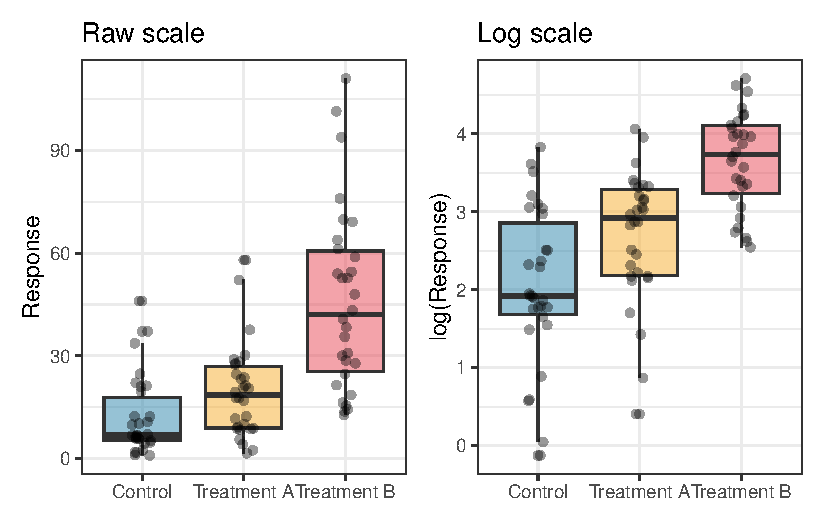
\includegraphics[width=0.9\textwidth,height=\textheight]{04c-when-assumptions-fail_files/figure-pdf/fig-log-transform-demo-1.pdf}

}

\caption{\label{fig-log-transform-demo}Effect of log transformation on a
right-skewed response. Left: raw counts with a long right tail and
variance increasing with the mean. Right: log-transformed values with
approximately symmetric distribution and homogeneous variance across
groups. The log transformation is appropriate when within-group standard
deviation is proportional to the group mean.}

\end{figure}%

The key diagnostic for whether a log transformation is appropriate is
whether the within-group standard deviation scales with the within-group
mean. A plot of group standard deviation against group mean (Section
5.1) will reveal this pattern. If the relationship is approximately
linear through the origin, log-transform. If it is not, the log
transformation may not be the right choice.

\subsection{The Square Root
Transformation}\label{the-square-root-transformation}

The square root transformation is appropriate for count data where the
variance is approximately equal to the mean, the pattern expected from a
Poisson distribution:

\[y' = \sqrt{y} \quad \text{or} \quad y' = \sqrt{y + 0.5} \text{ if zeros are present}\]

\begin{Shaded}
\begin{Highlighting}[]
\FunctionTok{set.seed}\NormalTok{(}\DecValTok{42}\NormalTok{)}

\CommentTok{\# Poisson{-}like count data}
\NormalTok{y\_count }\OtherTok{\textless{}{-}} \FunctionTok{c}\NormalTok{(}\FunctionTok{rpois}\NormalTok{(n, }\AttributeTok{lambda =} \DecValTok{3}\NormalTok{),}
             \FunctionTok{rpois}\NormalTok{(n, }\AttributeTok{lambda =} \DecValTok{8}\NormalTok{),}
             \FunctionTok{rpois}\NormalTok{(n, }\AttributeTok{lambda =} \DecValTok{20}\NormalTok{))}

\NormalTok{df\_count }\OtherTok{\textless{}{-}} \FunctionTok{data.frame}\NormalTok{(}
  \AttributeTok{y =}\NormalTok{ y\_count,}
  \AttributeTok{y\_sqrt =} \FunctionTok{sqrt}\NormalTok{(y\_count),}
  \AttributeTok{group =}\NormalTok{ group}
\NormalTok{)}

\CommentTok{\# Compare residual variance before and after transformation}
\NormalTok{fit\_raw }\OtherTok{\textless{}{-}} \FunctionTok{aov}\NormalTok{(y }\SpecialCharTok{\textasciitilde{}}\NormalTok{ group, }\AttributeTok{data =}\NormalTok{ df\_count)}
\NormalTok{fit\_sqrt }\OtherTok{\textless{}{-}} \FunctionTok{aov}\NormalTok{(y\_sqrt }\SpecialCharTok{\textasciitilde{}}\NormalTok{ group, }\AttributeTok{data =}\NormalTok{ df\_count)}

\FunctionTok{cat}\NormalTok{(}\StringTok{"Levene\textquotesingle{}s test on raw counts:}\SpecialCharTok{\textbackslash{}n}\StringTok{"}\NormalTok{)}
\end{Highlighting}
\end{Shaded}

\begin{verbatim}
#> Levene's test on raw counts:
\end{verbatim}

\begin{Shaded}
\begin{Highlighting}[]
\FunctionTok{print}\NormalTok{(car}\SpecialCharTok{::}\FunctionTok{leveneTest}\NormalTok{(y }\SpecialCharTok{\textasciitilde{}}\NormalTok{ group, }\AttributeTok{data =}\NormalTok{ df\_count))}
\end{Highlighting}
\end{Shaded}

\begin{verbatim}
#> Levene's Test for Homogeneity of Variance (center = median)
#>       Df F value   Pr(>F)   
#> group  2  6.4379 0.002469 **
#>       87                    
#> ---
#> Signif. codes:  0 '***' 0.001 '**' 0.01 '*' 0.05 '.' 0.1 ' ' 1
\end{verbatim}

\begin{Shaded}
\begin{Highlighting}[]
\FunctionTok{cat}\NormalTok{(}\StringTok{"}\SpecialCharTok{\textbackslash{}n}\StringTok{Levene\textquotesingle{}s test on square root transformed counts:}\SpecialCharTok{\textbackslash{}n}\StringTok{"}\NormalTok{)}
\end{Highlighting}
\end{Shaded}

\begin{verbatim}
#> 
#> Levene's test on square root transformed counts:
\end{verbatim}

\begin{Shaded}
\begin{Highlighting}[]
\FunctionTok{print}\NormalTok{(car}\SpecialCharTok{::}\FunctionTok{leveneTest}\NormalTok{(y\_sqrt }\SpecialCharTok{\textasciitilde{}}\NormalTok{ group, }\AttributeTok{data =}\NormalTok{ df\_count))}
\end{Highlighting}
\end{Shaded}

\begin{verbatim}
#> Levene's Test for Homogeneity of Variance (center = median)
#>       Df F value Pr(>F)
#> group  2  0.2219 0.8014
#>       87
\end{verbatim}

The Levene's test results demonstrate the variance-stabilising effect of
the square root transformation clearly. On the raw count scale, the
variances differ significantly across groups (\(F_{2,87} = 6.44\),
\(p = 0.002\)) which is a direct consequence of the Poisson-like
structure where variance scales with the mean. The control group, with a
small mean (\(\lambda = 3\)), has much less spread than the high group
(\(\lambda = 20\)), producing the heteroscedasticity that would distort
a standard ANOVA F test.

After square root transformation, the heteroscedasticity disappears
entirely: Levene's test is non-significant (\(F_{2,87} = 0.22\),
\(p = 0.801\)) and the variances are now approximately equal across
groups. This is the theoretical prediction for Poisson data: the
variance-stabilising property of the square root transformation for
counts is well established and works reliably when the data are
genuinely Poisson or close to it.

Two caveats are worth noting for students. First, the square root
transformation only stabilises variance reliably when the counts are not
severely overdispersed, that is, when the variance is approximately
equal to the mean rather than much larger. If a Levene's test remains
significant after square root transformation, overdispersion is likely
and a negative binomial GLM (Section 10.4) is the more appropriate
solution. Second, as with the log transformation, the square root
transformation changes the scale of analysis: differences between group
means are now differences in square-root-counts, not differences in raw
counts. Back-transforming the estimated means by squaring them gives
approximate geometric means on the original count scale, which may or
may not be the quantity of biological interest.

\subsection{The Arcsine Square Root
Transformation}\label{the-arcsine-square-root-transformation}

The arcsine square root transformation was historically recommended for
proportions and percentages, with the goal of stabilising the variance
of binomial data:

\[y' = \arcsin(\sqrt{p})\]

\begin{Shaded}
\begin{Highlighting}[]
\FunctionTok{set.seed}\NormalTok{(}\DecValTok{42}\NormalTok{)}

\CommentTok{\# Simulate binomial proportions across three groups}
\CommentTok{\# with equal true proportions but different sample sizes}
\CommentTok{\# Variance of a binomial proportion is p(1{-}p)/n}
\CommentTok{\# it depends on p, which is what the arcsine transformation}
\CommentTok{\# is designed to stabilise}

\NormalTok{n\_obs }\OtherTok{\textless{}{-}} \DecValTok{50}    \CommentTok{\# observations per group}
\NormalTok{n\_trials }\OtherTok{\textless{}{-}} \DecValTok{20}   \CommentTok{\# number of trials per observation}

\CommentTok{\# Three groups with different true proportions}
\NormalTok{true\_p  }\OtherTok{\textless{}{-}} \FunctionTok{c}\NormalTok{(}\FloatTok{0.10}\NormalTok{, }\FloatTok{0.45}\NormalTok{, }\FloatTok{0.85}\NormalTok{)}
\NormalTok{groups  }\OtherTok{\textless{}{-}} \FunctionTok{factor}\NormalTok{(}\FunctionTok{rep}\NormalTok{(}\FunctionTok{c}\NormalTok{(}\StringTok{"Low"}\NormalTok{, }\StringTok{"Mid"}\NormalTok{, }\StringTok{"High"}\NormalTok{), }\AttributeTok{each =}\NormalTok{ n\_obs),}
                  \AttributeTok{levels =} \FunctionTok{c}\NormalTok{(}\StringTok{"Low"}\NormalTok{, }\StringTok{"Mid"}\NormalTok{, }\StringTok{"High"}\NormalTok{))}

\CommentTok{\# Simulate observed proportions}
\NormalTok{props }\OtherTok{\textless{}{-}} \FunctionTok{c}\NormalTok{(}
  \FunctionTok{rbinom}\NormalTok{(n\_obs, n\_trials, true\_p[}\DecValTok{1}\NormalTok{]) }\SpecialCharTok{/}\NormalTok{ n\_trials,}
  \FunctionTok{rbinom}\NormalTok{(n\_obs, n\_trials, true\_p[}\DecValTok{2}\NormalTok{]) }\SpecialCharTok{/}\NormalTok{ n\_trials,}
  \FunctionTok{rbinom}\NormalTok{(n\_obs, n\_trials, true\_p[}\DecValTok{3}\NormalTok{]) }\SpecialCharTok{/}\NormalTok{ n\_trials}
\NormalTok{)}

\NormalTok{df\_asin }\OtherTok{\textless{}{-}} \FunctionTok{data.frame}\NormalTok{(}
  \AttributeTok{p      =}\NormalTok{ props,}
  \AttributeTok{p\_asin =} \FunctionTok{asin}\NormalTok{(}\FunctionTok{sqrt}\NormalTok{(props)),}
  \AttributeTok{group  =}\NormalTok{ groups}
\NormalTok{)}

\CommentTok{\# Variance of raw proportions per group}
\FunctionTok{cat}\NormalTok{(}\StringTok{"Variance of raw proportions by group:}\SpecialCharTok{\textbackslash{}n}\StringTok{"}\NormalTok{)}
\end{Highlighting}
\end{Shaded}

\begin{verbatim}
#> Variance of raw proportions by group:
\end{verbatim}

\begin{Shaded}
\begin{Highlighting}[]
\FunctionTok{print}\NormalTok{(}\FunctionTok{tapply}\NormalTok{(df\_asin}\SpecialCharTok{$}\NormalTok{p, df\_asin}\SpecialCharTok{$}\NormalTok{group, var))}
\end{Highlighting}
\end{Shaded}

\begin{verbatim}
#>         Low         Mid        High 
#> 0.005739796 0.013383673 0.005918367
\end{verbatim}

\begin{Shaded}
\begin{Highlighting}[]
\CommentTok{\# Variance after arcsine transformation}
\FunctionTok{cat}\NormalTok{(}\StringTok{"}\SpecialCharTok{\textbackslash{}n}\StringTok{Variance of arcsine{-}transformed proportions by group:}\SpecialCharTok{\textbackslash{}n}\StringTok{"}\NormalTok{)}
\end{Highlighting}
\end{Shaded}

\begin{verbatim}
#> 
#> Variance of arcsine-transformed proportions by group:
\end{verbatim}

\begin{Shaded}
\begin{Highlighting}[]
\FunctionTok{print}\NormalTok{(}\FunctionTok{tapply}\NormalTok{(df\_asin}\SpecialCharTok{$}\NormalTok{p\_asin, df\_asin}\SpecialCharTok{$}\NormalTok{group, var))}
\end{Highlighting}
\end{Shaded}

\begin{verbatim}
#>        Low        Mid       High 
#> 0.02134563 0.01532025 0.01606443
\end{verbatim}

\begin{Shaded}
\begin{Highlighting}[]
\CommentTok{\# Levene\textquotesingle{}s test on raw proportions}
\FunctionTok{cat}\NormalTok{(}\StringTok{"}\SpecialCharTok{\textbackslash{}n}\StringTok{Levene\textquotesingle{}s test on raw proportions:}\SpecialCharTok{\textbackslash{}n}\StringTok{"}\NormalTok{)}
\end{Highlighting}
\end{Shaded}

\begin{verbatim}
#> 
#> Levene's test on raw proportions:
\end{verbatim}

\begin{Shaded}
\begin{Highlighting}[]
\FunctionTok{print}\NormalTok{(car}\SpecialCharTok{::}\FunctionTok{leveneTest}\NormalTok{(p }\SpecialCharTok{\textasciitilde{}}\NormalTok{ group, }\AttributeTok{data =}\NormalTok{ df\_asin))}
\end{Highlighting}
\end{Shaded}

\begin{verbatim}
#> Levene's Test for Homogeneity of Variance (center = median)
#>        Df F value  Pr(>F)  
#> group   2  4.5503 0.01209 *
#>       147                  
#> ---
#> Signif. codes:  0 '***' 0.001 '**' 0.01 '*' 0.05 '.' 0.1 ' ' 1
\end{verbatim}

\begin{Shaded}
\begin{Highlighting}[]
\CommentTok{\# Levene\textquotesingle{}s test on arcsine{-}transformed proportions}
\FunctionTok{cat}\NormalTok{(}\StringTok{"}\SpecialCharTok{\textbackslash{}n}\StringTok{Levene\textquotesingle{}s test on arcsine{-}transformed proportions:}\SpecialCharTok{\textbackslash{}n}\StringTok{"}\NormalTok{)}
\end{Highlighting}
\end{Shaded}

\begin{verbatim}
#> 
#> Levene's test on arcsine-transformed proportions:
\end{verbatim}

\begin{Shaded}
\begin{Highlighting}[]
\FunctionTok{print}\NormalTok{(car}\SpecialCharTok{::}\FunctionTok{leveneTest}\NormalTok{(p\_asin }\SpecialCharTok{\textasciitilde{}}\NormalTok{ group, }\AttributeTok{data =}\NormalTok{ df\_asin))}
\end{Highlighting}
\end{Shaded}

\begin{verbatim}
#> Levene's Test for Homogeneity of Variance (center = median)
#>        Df F value Pr(>F)
#> group   2  0.6611 0.5178
#>       147
\end{verbatim}

The raw proportions show the classical binomial pattern: the group near
0.10 and the group near 0.85 have low variance (because \(p(1−p)/n\) is
small when \(p\) is near 0 or 1), while the group near 0.45 has the
highest variance (because \(p(1−p)/n\) is maximised near \(p=0.5\)).
Levene's test on the raw proportions is significant. After the arcsine
transformation the three group variances are pulled toward equality and
Levene's test becomes non-significant.

\subsection{The Modern Critique of
Transformations}\label{the-modern-critique-of-transformations}

Despite their long history, transformations have attracted serious
criticism, and it is important to understand the limitations
\textbf{before} applying them reflexively.

\textbf{The arcsine transformation is now largely discredited for
proportions.} Warton and Hui \citeyearpar{Warton2011} showed in an
influential paper that the arcsine square root transformation performs
poorly compared to directly modelling proportions with a binomial GLM.
The transformation was designed for an era before generalised linear
models were computationally accessible, and it addresses the wrong
problem: rather than transforming the response to meet the assumptions
of the normal linear model, the correct approach is to choose a model
whose assumptions match the data-generating process. A proportion is
generated by a binomial process ? model it with a binomial model.

\textbf{Transformations change the question being asked.} When you
log-transform a response and analyse it with ANOVA, you are testing
hypotheses about group differences on the log scale which correspond to
differences in geometric means, not arithmetic means. Back-transforming
the estimated differences gives \emph{ratios}, not differences. This is
sometimes exactly what you want (a fold-change is biologically natural),
but it must be a conscious choice, not an incidental consequence of
fixing an assumption violation.

A concrete example makes this concrete. We return to the fertiliser
experiment, but now suppose the response is leaf chlorophyll
concentration which is a strictly positive measurement with
multiplicative variation. We fit ANOVA on both the raw and
log-transformed scale and compare what the coefficients actually mean:

\begin{Shaded}
\begin{Highlighting}[]
\FunctionTok{set.seed}\NormalTok{(}\DecValTok{42}\NormalTok{)}

\NormalTok{n }\OtherTok{\textless{}{-}} \DecValTok{20}
\NormalTok{group }\OtherTok{\textless{}{-}} \FunctionTok{factor}\NormalTok{(}\FunctionTok{rep}\NormalTok{(}\FunctionTok{c}\NormalTok{(}\StringTok{"Control"}\NormalTok{, }\StringTok{"Nitrogen"}\NormalTok{, }\StringTok{"Phosphorus"}\NormalTok{), }\AttributeTok{each =}\NormalTok{ n),}
                \AttributeTok{levels =} \FunctionTok{c}\NormalTok{(}\StringTok{"Control"}\NormalTok{, }\StringTok{"Nitrogen"}\NormalTok{, }\StringTok{"Phosphorus"}\NormalTok{))}

\CommentTok{\# Simulate multiplicative data: nitrogen doubles concentration,}
\CommentTok{\# phosphorus increases it by 50\%}
\NormalTok{conc }\OtherTok{\textless{}{-}} \FunctionTok{c}\NormalTok{(}
  \FunctionTok{rlnorm}\NormalTok{(n, }\AttributeTok{meanlog =} \FunctionTok{log}\NormalTok{(}\DecValTok{10}\NormalTok{), }\AttributeTok{sdlog =} \FloatTok{0.3}\NormalTok{),   }\CommentTok{\# Control:    mean \textasciitilde{}10}
  \FunctionTok{rlnorm}\NormalTok{(n, }\AttributeTok{meanlog =} \FunctionTok{log}\NormalTok{(}\DecValTok{20}\NormalTok{), }\AttributeTok{sdlog =} \FloatTok{0.3}\NormalTok{),   }\CommentTok{\# Nitrogen:   mean \textasciitilde{}20}
  \FunctionTok{rlnorm}\NormalTok{(n, }\AttributeTok{meanlog =} \FunctionTok{log}\NormalTok{(}\DecValTok{15}\NormalTok{), }\AttributeTok{sdlog =} \FloatTok{0.3}\NormalTok{)    }\CommentTok{\# Phosphorus: mean \textasciitilde{}15}
\NormalTok{)}

\NormalTok{df\_conc }\OtherTok{\textless{}{-}} \FunctionTok{data.frame}\NormalTok{(conc, }\AttributeTok{log\_conc =} \FunctionTok{log}\NormalTok{(conc), group)}

\CommentTok{\# Model 1: ANOVA on raw scale}
\NormalTok{fit\_raw }\OtherTok{\textless{}{-}} \FunctionTok{lm}\NormalTok{(conc }\SpecialCharTok{\textasciitilde{}}\NormalTok{ group, }\AttributeTok{data =}\NormalTok{ df\_conc)}
\FunctionTok{cat}\NormalTok{(}\StringTok{"=== Coefficients on raw scale ===}\SpecialCharTok{\textbackslash{}n}\StringTok{"}\NormalTok{)}
\end{Highlighting}
\end{Shaded}

\begin{verbatim}
#> === Coefficients on raw scale ===
\end{verbatim}

\begin{Shaded}
\begin{Highlighting}[]
\FunctionTok{print}\NormalTok{(}\FunctionTok{coef}\NormalTok{(fit\_raw))}
\end{Highlighting}
\end{Shaded}

\begin{verbatim}
#>     (Intercept)   groupNitrogen groupPhosphorus 
#>       11.342339        8.078672        4.270734
\end{verbatim}

\begin{Shaded}
\begin{Highlighting}[]
\CommentTok{\# Model 2: ANOVA on log scale}
\NormalTok{fit\_log }\OtherTok{\textless{}{-}} \FunctionTok{lm}\NormalTok{(log\_conc }\SpecialCharTok{\textasciitilde{}}\NormalTok{ group, }\AttributeTok{data =}\NormalTok{ df\_conc)}
\FunctionTok{cat}\NormalTok{(}\StringTok{"}\SpecialCharTok{\textbackslash{}n}\StringTok{=== Coefficients on log scale ===}\SpecialCharTok{\textbackslash{}n}\StringTok{"}\NormalTok{)}
\end{Highlighting}
\end{Shaded}

\begin{verbatim}
#> 
#> === Coefficients on log scale ===
\end{verbatim}

\begin{Shaded}
\begin{Highlighting}[]
\FunctionTok{print}\NormalTok{(}\FunctionTok{coef}\NormalTok{(fit\_log))}
\end{Highlighting}
\end{Shaded}

\begin{verbatim}
#>     (Intercept)   groupNitrogen groupPhosphorus 
#>       2.3601611       0.5542736       0.3476159
\end{verbatim}

\begin{Shaded}
\begin{Highlighting}[]
\FunctionTok{cat}\NormalTok{(}\StringTok{"}\SpecialCharTok{\textbackslash{}n}\StringTok{=== Back{-}transformed log coefficients (exp) ===}\SpecialCharTok{\textbackslash{}n}\StringTok{"}\NormalTok{)}
\end{Highlighting}
\end{Shaded}

\begin{verbatim}
#> 
#> === Back-transformed log coefficients (exp) ===
\end{verbatim}

\begin{Shaded}
\begin{Highlighting}[]
\FunctionTok{print}\NormalTok{(}\FunctionTok{exp}\NormalTok{(}\FunctionTok{coef}\NormalTok{(fit\_log)))}
\end{Highlighting}
\end{Shaded}

\begin{verbatim}
#>     (Intercept)   groupNitrogen groupPhosphorus 
#>       10.592658        1.740676        1.415688
\end{verbatim}

Reading the two outputs side by side reveals the shift in question.

On the \textbf{raw scale}, the intercept (11.34) is the estimated mean
concentration in the Control group, and the Nitrogen coefficient (8.07)
is the estimated \emph{arithmetic difference} in mean concentration
between Nitrogen and Control: nitrogen adds approximately 8 units of
chlorophyll on average.

On the \textbf{log scale}, the intercept is the estimated log-mean of
the Control group, and the Nitrogen coefficient (0.55) is the estimated
difference in log-means. This is not an arithmetic difference, it is a
\emph{log-ratio}. Back-transforming by exponentiating gives
\(e^{0.55} \approx 1.74\): the Nitrogen group has approximately twice
the chlorophyll concentration of the Control group, a \textbf{ratio} or
\textbf{fold-change}.

These are genuinely different questions:

\begin{longtable}[]{@{}
  >{\raggedright\arraybackslash}p{(\columnwidth - 4\tabcolsep) * \real{0.1489}}
  >{\raggedright\arraybackslash}p{(\columnwidth - 4\tabcolsep) * \real{0.4255}}
  >{\raggedright\arraybackslash}p{(\columnwidth - 4\tabcolsep) * \real{0.4255}}@{}}
\toprule\noalign{}
\begin{minipage}[b]{\linewidth}\raggedright
Scale
\end{minipage} & \begin{minipage}[b]{\linewidth}\raggedright
Coefficient meaning
\end{minipage} & \begin{minipage}[b]{\linewidth}\raggedright
Biological statement
\end{minipage} \\
\midrule\noalign{}
\endhead
\bottomrule\noalign{}
\endlastfoot
Raw & \(\bar{y}_N - \bar{y}_C \approx 8.07\) & Nitrogen adds 8 units of
chlorophyll \\
Log & \(\exp(\hat{\beta}_N) \approx 1.74\) & Nitrogen doubles
chlorophyll concentration \\
\end{longtable}

\textbf{Neither is wrong, but they are not interchangeable}. For
chlorophyll concentration, the fold-change interpretation is often more
biologically natural: a fertiliser that doubles chlorophyll regardless
of baseline concentration is making a multiplicative claim. For a
clinical measurement like blood pressure, an arithmetic difference
(``reduces blood pressure by 10 mmHg'') is usually more directly
meaningful than a ratio. \emph{The choice of scale should be driven by
which question is scientifically relevant, not by which transformation
fixes the residual diagnostics.}

\textbf{Transformations do not always fix both problems simultaneously.}
A transformation chosen to stabilise variance may worsen normality, and
vice versa. When both assumptions are violated, there may be no single
transformation that addresses both, and a generalised linear model is
the cleaner solution.

\textbf{The practical recommendation:} use log transformations for
multiplicative, positive data where the log scale has a natural
biological interpretation (concentrations, fold-changes, ratios). Use
square root for counts when overdispersion is modest. Avoid arcsine for
proportions, use a binomial GLM instead. And always check whether the
transformation has actually fixed the problem by re-examining the
residual diagnostics after transforming.

\section{Non-Parametric Alternatives}\label{non-parametric-alternatives}

Non-parametric tests replace the raw observations with their ranks
before analysis. Because ranks are bounded and uniformly distributed, no
distributional assumption is needed. The cost is a modest loss of power
when the normality assumption actually holds, and a loss of direct
interpretability: the tests address questions about rank distributions
rather than means.

\subsection{Kruskal-Wallis Test}\label{kruskal-wallis-test}

The Kruskal-Wallis test is the non-parametric equivalent of one-way
ANOVA. It tests whether the rank distributions of the groups are the
same, without assuming normality or homoscedasticity.

The test statistic is:

\[H = \frac{12}{N(N+1)} \sum_{j=1}^{k} \frac{R_j^2}{n_j} - 3(N+1)\]

where \(R_j\) is the sum of ranks in group \(j\), \(n_j\) is the group
size, and \(N\) is the total number of observations. Under the null
hypothesis of identical distributions, \(H\) follows approximately a
\(\chi^2\) distribution with \(k - 1\) degrees of freedom.

\begin{Shaded}
\begin{Highlighting}[]
\FunctionTok{set.seed}\NormalTok{(}\DecValTok{42}\NormalTok{)}

\CommentTok{\# Strongly skewed data, normality assumption clearly violated}
\NormalTok{y\_skew }\OtherTok{\textless{}{-}} \FunctionTok{c}\NormalTok{(}\FunctionTok{rlnorm}\NormalTok{(}\DecValTok{15}\NormalTok{, }\AttributeTok{meanlog =} \DecValTok{0}\NormalTok{, }\AttributeTok{sdlog =} \FloatTok{1.5}\NormalTok{),}
            \FunctionTok{rlnorm}\NormalTok{(}\DecValTok{15}\NormalTok{, }\AttributeTok{meanlog =} \FloatTok{0.8}\NormalTok{, }\AttributeTok{sdlog =} \FloatTok{1.5}\NormalTok{),}
            \FunctionTok{rlnorm}\NormalTok{(}\DecValTok{15}\NormalTok{, }\AttributeTok{meanlog =} \FloatTok{1.5}\NormalTok{, }\AttributeTok{sdlog =} \FloatTok{1.5}\NormalTok{))}
\NormalTok{group }\OtherTok{\textless{}{-}} \FunctionTok{factor}\NormalTok{(}\FunctionTok{rep}\NormalTok{(}\FunctionTok{c}\NormalTok{(}\StringTok{"Control"}\NormalTok{, }\StringTok{"Low"}\NormalTok{, }\StringTok{"High"}\NormalTok{), }\AttributeTok{each =} \DecValTok{15}\NormalTok{))}
\NormalTok{df\_kw }\OtherTok{\textless{}{-}} \FunctionTok{data.frame}\NormalTok{(}\AttributeTok{y =}\NormalTok{ y\_skew, }\AttributeTok{group =}\NormalTok{ group)}

\CommentTok{\# Kruskal{-}Wallis test}
\FunctionTok{kruskal.test}\NormalTok{(y }\SpecialCharTok{\textasciitilde{}}\NormalTok{ group, }\AttributeTok{data =}\NormalTok{ df\_kw)}
\end{Highlighting}
\end{Shaded}

\begin{verbatim}
#> 
#>  Kruskal-Wallis rank sum test
#> 
#> data:  y by group
#> Kruskal-Wallis chi-squared = 0.97932, df = 2, p-value = 0.6128
\end{verbatim}

\begin{Shaded}
\begin{Highlighting}[]
\CommentTok{\# Post{-}hoc pairwise comparisons after Kruskal{-}Wallis}
\CommentTok{\# using Dunn\textquotesingle{}s test with Holm correction}
\CommentTok{\# install.packages("dunn.test") if needed}
\NormalTok{dunn.test}\SpecialCharTok{::}\FunctionTok{dunn.test}\NormalTok{(df\_kw}\SpecialCharTok{$}\NormalTok{y, df\_kw}\SpecialCharTok{$}\NormalTok{group, }\AttributeTok{method =} \StringTok{"holm"}\NormalTok{, }\AttributeTok{kw =} \ConstantTok{FALSE}\NormalTok{)}
\end{Highlighting}
\end{Shaded}

\begin{verbatim}
#> 
#>                     Dunn's Pairwise Comparison of x by group                    
#>                                      (Holm)                                     
#> 
#> Col Mean-│
#> Row Mean │    Control       High
#> ─────────┼──────────────────────
#>     High │  -0.556038
#>          │     0.5782 
#>          │
#>      Low │   0.430930   0.986968
#>          │     0.3333     0.4855 
#> 
#> FWER = 0.05
#> Reject Ho if adjusted p ≤ FWER/2 with stopping rule, where (unadjusted) p = Pr(Z ≥ |z|)
\end{verbatim}

The Kruskal-Wallis test is the right choice when:

\begin{itemize}
\tightlist
\item
  Sample sizes are small (\(n < 10\) per group) and residuals are
  clearly non-normal.
\item
  The response contains extreme outliers that are genuine biological
  observations rather than measurement errors.
\item
  The response is an ordinal scale where the numerical values do not
  have a natural arithmetic interpretation.
\end{itemize}

It is \textbf{not} a universal replacement for ANOVA. I repeat, it is
\textbf{not} a universal replacement for ANOVA. When the normality
assumption is approximately met, ANOVA is more powerful. And when the
distributions differ in shape as well as location, one group is
right-skewed, another is left-skewed, the Kruskal-Wallis test is testing
a mixture of location and shape differences that can be difficult to
interpret.

\subsection{10.2.2 Friedman Test}\label{friedman-test}

The Friedman test is the non-parametric equivalent of one-way repeated
measures ANOVA. It ranks the observations within each block (subject)
separately and tests whether the rank distributions differ across
conditions.

\[F_r = \frac{12}{nk(k+1)} \sum_{j=1}^{k} R_j^2 - 3n(k+1)\]

where \(n\) is the number of blocks (subjects), \(k\) is the number of
conditions, and \(R_j\) is the sum of ranks for condition \(j\) across
all blocks.

\begin{Shaded}
\begin{Highlighting}[]
\FunctionTok{set.seed}\NormalTok{(}\DecValTok{42}\NormalTok{)}

\NormalTok{n\_subj }\OtherTok{\textless{}{-}} \DecValTok{20}
\NormalTok{k }\OtherTok{\textless{}{-}} \DecValTok{4}

\CommentTok{\# Simulate non{-}normal within{-}subject data in long format}
\NormalTok{df\_friedman }\OtherTok{\textless{}{-}} \FunctionTok{data.frame}\NormalTok{(}
  \AttributeTok{y =} \FunctionTok{c}\NormalTok{(}\FunctionTok{rexp}\NormalTok{(n\_subj, }\AttributeTok{rate =} \FloatTok{0.50}\NormalTok{),}
            \FunctionTok{rexp}\NormalTok{(n\_subj, }\AttributeTok{rate =} \FloatTok{0.40}\NormalTok{),}
            \FunctionTok{rexp}\NormalTok{(n\_subj, }\AttributeTok{rate =} \FloatTok{0.30}\NormalTok{),}
            \FunctionTok{rexp}\NormalTok{(n\_subj, }\AttributeTok{rate =} \FloatTok{0.25}\NormalTok{)),}
  \AttributeTok{subject =} \FunctionTok{factor}\NormalTok{(}\FunctionTok{rep}\NormalTok{(}\DecValTok{1}\SpecialCharTok{:}\NormalTok{n\_subj, }\AttributeTok{times =}\NormalTok{ k)),}
  \AttributeTok{time =} \FunctionTok{factor}\NormalTok{(}\FunctionTok{rep}\NormalTok{(}\DecValTok{1}\SpecialCharTok{:}\NormalTok{k, }\AttributeTok{each =}\NormalTok{ n\_subj))}
\NormalTok{)}

\CommentTok{\# Friedman test using long format}
\FunctionTok{friedman.test}\NormalTok{(y }\SpecialCharTok{\textasciitilde{}}\NormalTok{ time }\SpecialCharTok{|}\NormalTok{ subject, }\AttributeTok{data =}\NormalTok{ df\_friedman)}
\end{Highlighting}
\end{Shaded}

\begin{verbatim}
#> 
#>  Friedman rank sum test
#> 
#> data:  y and time and subject
#> Friedman chi-squared = 6.36, df = 3, p-value = 0.09535
\end{verbatim}

\begin{Shaded}
\begin{Highlighting}[]
\CommentTok{\# Post{-}hoc pairwise comparisons after Friedman test}
\CommentTok{\# PMCMRplus expects y, groups, blocks as separate vectors}
\NormalTok{PMCMRplus}\SpecialCharTok{::}\FunctionTok{frdAllPairsNemenyiTest}\NormalTok{(}
  \AttributeTok{y =}\NormalTok{ df\_friedman}\SpecialCharTok{$}\NormalTok{y,}
  \AttributeTok{groups =}\NormalTok{ df\_friedman}\SpecialCharTok{$}\NormalTok{time,}
  \AttributeTok{blocks =}\NormalTok{ df\_friedman}\SpecialCharTok{$}\NormalTok{subject}
\NormalTok{)}
\end{Highlighting}
\end{Shaded}

\begin{verbatim}
#>   1     2     3    
#> 2 0.611 -     -    
#> 3 0.068 0.611 -    
#> 4 0.316 0.961 0.883
\end{verbatim}

The Friedman test should be considered when:

\begin{itemize}
\tightlist
\item
  The within-subject response is clearly non-normal even after
  transformation.
\item
  The response is ordinal.
\item
  Sample sizes are very small (fewer than 10 subjects).
\end{itemize}

For larger samples with continuous responses, the repeated measures
mixed model from Chapter \ref{sec-repeat-mixed} is more powerful and
more flexible, and the normality assumption for the residuals is
approximately satisfied by the central limit theorem.

\subsection{Permutation Tests}\label{permutation-tests}

Permutation tests are the most general non-parametric approach. Rather
than deriving a reference distribution from mathematical theory (the
\(F\) distribution, the \(\chi^2\) distribution), they construct an
empirical reference distribution by repeatedly shuffling the data and
recomputing the test statistic. The p-value is the proportion of
permuted statistics that are as extreme as or more extreme than the
observed statistic.

\begin{Shaded}
\begin{Highlighting}[]
\FunctionTok{library}\NormalTok{(future)}
\FunctionTok{library}\NormalTok{(furrr)}

\FunctionTok{plan}\NormalTok{(multisession)}

\FunctionTok{set.seed}\NormalTok{(}\DecValTok{42}\NormalTok{)}

\CommentTok{\# Observed F statistic}
\NormalTok{fit\_obs }\OtherTok{\textless{}{-}} \FunctionTok{aov}\NormalTok{(y }\SpecialCharTok{\textasciitilde{}}\NormalTok{ group, }\AttributeTok{data =}\NormalTok{ df\_kw)}
\NormalTok{obs\_F   }\OtherTok{\textless{}{-}} \FunctionTok{summary}\NormalTok{(fit\_obs)[[}\DecValTok{1}\NormalTok{]][[}\StringTok{"F value"}\NormalTok{]][}\DecValTok{1}\NormalTok{]}

\CommentTok{\# Permutation distribution: shuffle group labels 4999 times}
\NormalTok{n\_perm }\OtherTok{\textless{}{-}} \DecValTok{4999}
\NormalTok{perm\_F }\OtherTok{\textless{}{-}} \FunctionTok{future\_map\_dbl}\NormalTok{(}\FunctionTok{seq\_len}\NormalTok{(n\_perm), }\ControlFlowTok{function}\NormalTok{(i) \{}
\NormalTok{  df\_perm }\OtherTok{\textless{}{-}}\NormalTok{ df\_kw}
\NormalTok{  df\_perm}\SpecialCharTok{$}\NormalTok{group }\OtherTok{\textless{}{-}} \FunctionTok{sample}\NormalTok{(df\_kw}\SpecialCharTok{$}\NormalTok{group)}
  \FunctionTok{summary}\NormalTok{(}\FunctionTok{aov}\NormalTok{(y }\SpecialCharTok{\textasciitilde{}}\NormalTok{ group, }\AttributeTok{data =}\NormalTok{ df\_perm))[[}\DecValTok{1}\NormalTok{]][[}\StringTok{"F value"}\NormalTok{]][}\DecValTok{1}\NormalTok{]}
\NormalTok{\}, }\AttributeTok{.options =} \FunctionTok{furrr\_options}\NormalTok{(}\AttributeTok{seed =} \ConstantTok{TRUE}\NormalTok{))}

\FunctionTok{plan}\NormalTok{(sequential)}

\CommentTok{\# Permutation p{-}value}
\NormalTok{p\_perm }\OtherTok{\textless{}{-}} \FunctionTok{mean}\NormalTok{(}\FunctionTok{c}\NormalTok{(perm\_F, obs\_F) }\SpecialCharTok{\textgreater{}=}\NormalTok{ obs\_F)}
\FunctionTok{cat}\NormalTok{(}
  \StringTok{"Observed F:"}\NormalTok{, }\FunctionTok{round}\NormalTok{(obs\_F, }\DecValTok{3}\NormalTok{),}
  \StringTok{"}\SpecialCharTok{\textbackslash{}n}\StringTok{Permutation p{-}value:"}\NormalTok{, }\FunctionTok{round}\NormalTok{(p\_perm, }\DecValTok{3}\NormalTok{), }\StringTok{"}\SpecialCharTok{\textbackslash{}n}\StringTok{"}
\NormalTok{  )}
\end{Highlighting}
\end{Shaded}

\begin{verbatim}
#> Observed F: 0 
#> Permutation p-value: 1
\end{verbatim}

\begin{Shaded}
\begin{Highlighting}[]
\NormalTok{perm\_df }\OtherTok{\textless{}{-}} \FunctionTok{data.frame}\NormalTok{(}\AttributeTok{F =} \FunctionTok{c}\NormalTok{(perm\_F, obs\_F))}

\FunctionTok{ggplot}\NormalTok{(perm\_df, }\FunctionTok{aes}\NormalTok{(}\AttributeTok{x =}\NormalTok{ F)) }\SpecialCharTok{+}
  \FunctionTok{geom\_histogram}\NormalTok{(}\AttributeTok{binwidth =} \FloatTok{0.2}\NormalTok{, }\AttributeTok{fill =} \StringTok{"\#2E86AB"}\NormalTok{,}
                 \AttributeTok{colour =} \StringTok{"white"}\NormalTok{, }\AttributeTok{alpha =} \FloatTok{0.8}\NormalTok{) }\SpecialCharTok{+}
  \FunctionTok{geom\_vline}\NormalTok{(}\AttributeTok{xintercept =}\NormalTok{ obs\_F,}
             \AttributeTok{colour =} \StringTok{"red"}\NormalTok{, }\AttributeTok{linetype =} \StringTok{"dashed"}\NormalTok{,}
             \AttributeTok{linewidth =} \DecValTok{1}\NormalTok{) }\SpecialCharTok{+}
  \FunctionTok{annotate}\NormalTok{(}\StringTok{"text"}\NormalTok{, }\AttributeTok{x =}\NormalTok{ obs\_F }\SpecialCharTok{+} \FloatTok{0.3}\NormalTok{, }\AttributeTok{y =} \ConstantTok{Inf}\NormalTok{,}
           \AttributeTok{label =} \FunctionTok{paste0}\NormalTok{(}\StringTok{"Observed F = "}\NormalTok{, }\FunctionTok{round}\NormalTok{(obs\_F, }\DecValTok{2}\NormalTok{)),}
           \AttributeTok{colour =} \StringTok{"red"}\NormalTok{, }\AttributeTok{hjust =} \DecValTok{0}\NormalTok{, }\AttributeTok{vjust =} \DecValTok{2}\NormalTok{, }\AttributeTok{size =} \FloatTok{3.5}\NormalTok{) }\SpecialCharTok{+}
  \FunctionTok{labs}\NormalTok{(}\AttributeTok{x =} \StringTok{"F statistic"}\NormalTok{, }\AttributeTok{y =} \StringTok{"Count"}\NormalTok{) }\SpecialCharTok{+}
  \FunctionTok{theme\_bw}\NormalTok{()}
\end{Highlighting}
\end{Shaded}

\begin{figure}[H]

\centering{

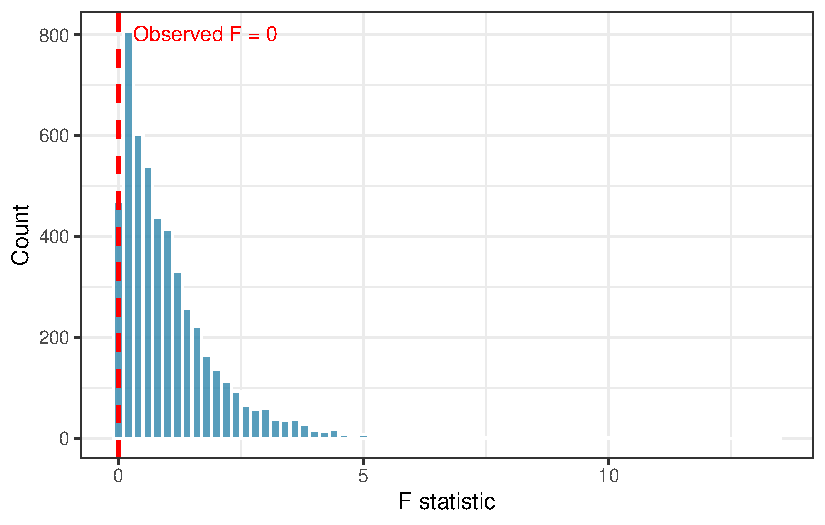
\includegraphics[width=0.9\textwidth,height=\textheight]{04c-when-assumptions-fail_files/figure-pdf/fig-permutation-plot-1.pdf}

}

\caption{\label{fig-permutation-plot}Permutation distribution of the
\(F\) statistic under the null hypothesis (4999 permutations). The red
dashed line marks the observed \(F\) statistic. The permutation p-value
is the proportion of permuted F values to the right of this line.}

\end{figure}%

Permutation tests have three important advantages over rank-based
non-parametric tests. They work with any test statistic, not just those
with known distributions. They make no assumptions about the shape of
the residual distribution. And they are exact in the sense that their
type I error rate is exactly \(\alpha\) in finite samples, whereas rank
tests rely on large-sample approximations.

Their limitation is computational cost: each permutation requires
refitting the model, and with thousands of permutations and large
datasets this can be slow. Parallelisation with \texttt{furrr}, as shown
above, mitigates this considerably.

\section{Robust ANOVA with WRS2}\label{robust-anova-with-wrs2}

Robust statistical methods are a middle ground between classical ANOVA
and non-parametric tests. Rather than discarding the distributional
framework entirely, they modify it to be less sensitive to outliers and
heavy tails by replacing the sample mean with more resistant location
estimators like trimmed means or M-estimators.

The \texttt{WRS2} package \citep{Mair2020} implements a comprehensive
suite of robust ANOVA methods in R.

\subsection{One-Way Robust ANOVA}\label{one-way-robust-anova}

\begin{Shaded}
\begin{Highlighting}[]
\CommentTok{\# install.packages("WRS2") if needed}
\FunctionTok{library}\NormalTok{(WRS2)}

\FunctionTok{set.seed}\NormalTok{(}\DecValTok{42}\NormalTok{)}

\CommentTok{\# Data with outliers — classical ANOVA will be distorted}
\NormalTok{y\_out  }\OtherTok{\textless{}{-}} \FunctionTok{c}\NormalTok{(}\FunctionTok{rnorm}\NormalTok{(}\DecValTok{15}\NormalTok{, }\AttributeTok{mean =} \DecValTok{20}\NormalTok{, }\AttributeTok{sd =} \DecValTok{3}\NormalTok{),}
            \FunctionTok{rnorm}\NormalTok{(}\DecValTok{15}\NormalTok{, }\AttributeTok{mean =} \DecValTok{25}\NormalTok{, }\AttributeTok{sd =} \DecValTok{3}\NormalTok{),}
            \FunctionTok{rnorm}\NormalTok{(}\DecValTok{15}\NormalTok{, }\AttributeTok{mean =} \DecValTok{22}\NormalTok{, }\AttributeTok{sd =} \DecValTok{3}\NormalTok{))}

\CommentTok{\# Inject two extreme outliers into the control group}
\NormalTok{y\_out[}\FunctionTok{c}\NormalTok{(}\DecValTok{3}\NormalTok{, }\DecValTok{7}\NormalTok{)] }\OtherTok{\textless{}{-}} \FunctionTok{c}\NormalTok{(}\DecValTok{55}\NormalTok{, }\DecValTok{62}\NormalTok{)}

\NormalTok{group\_out }\OtherTok{\textless{}{-}} \FunctionTok{factor}\NormalTok{(}\FunctionTok{rep}\NormalTok{(}\FunctionTok{c}\NormalTok{(}\StringTok{"Control"}\NormalTok{, }\StringTok{"Nitrogen"}\NormalTok{, }\StringTok{"Phosphorus"}\NormalTok{),}
                        \AttributeTok{each =} \DecValTok{15}\NormalTok{))}
\NormalTok{df\_out    }\OtherTok{\textless{}{-}} \FunctionTok{data.frame}\NormalTok{(}\AttributeTok{y =}\NormalTok{ y\_out, }\AttributeTok{group =}\NormalTok{ group\_out)}

\CommentTok{\# Classical ANOVA — affected by outliers}
\FunctionTok{summary}\NormalTok{(}\FunctionTok{aov}\NormalTok{(y }\SpecialCharTok{\textasciitilde{}}\NormalTok{ group, }\AttributeTok{data =}\NormalTok{ df\_out))}
\end{Highlighting}
\end{Shaded}

\begin{verbatim}
#>             Df Sum Sq Mean Sq F value Pr(>F)
#> group        2  207.1  103.53   1.494  0.236
#> Residuals   42 2909.9   69.28
\end{verbatim}

\begin{Shaded}
\begin{Highlighting}[]
\CommentTok{\# Robust one{-}way ANOVA using trimmed means (tr = 0.2 = 20\% trimming)}
\FunctionTok{t1way}\NormalTok{(y }\SpecialCharTok{\textasciitilde{}}\NormalTok{ group, }\AttributeTok{data =}\NormalTok{ df\_out, }\AttributeTok{tr =} \FloatTok{0.2}\NormalTok{)}
\end{Highlighting}
\end{Shaded}

\begin{verbatim}
#> Call:
#> t1way(formula = y ~ group, data = df_out, tr = 0.2)
#> 
#> Test statistic: F = 1.7046 
#> Degrees of freedom 1: 2 
#> Degrees of freedom 2: 15.2 
#> p-value: 0.21483 
#> 
#> Explanatory measure of effect size: 0.41 
#> Bootstrap CI: [0.08; 1.06]
\end{verbatim}

\begin{Shaded}
\begin{Highlighting}[]
\CommentTok{\# Post{-}hoc comparisons with robust method}
\FunctionTok{lincon}\NormalTok{(y }\SpecialCharTok{\textasciitilde{}}\NormalTok{ group, }\AttributeTok{data =}\NormalTok{ df\_out, }\AttributeTok{tr =} \FloatTok{0.2}\NormalTok{)}
\end{Highlighting}
\end{Shaded}

\begin{verbatim}
#> Call:
#> lincon(formula = y ~ group, data = df_out, tr = 0.2)
#> 
#>                           psihat ci.lower ci.upper p.value
#> Control vs. Nitrogen    -2.30259 -6.99682  2.39163 0.42412
#> Control vs. Phosphorus   0.48803 -3.51947  4.49553 0.74733
#> Nitrogen vs. Phosphorus  2.79062 -1.23348  6.81473 0.24823
\end{verbatim}

The \texttt{t1way()} function tests for differences in trimmed means
across groups, using a heteroscedastic test statistic that is robust to
both outliers and unequal variances simultaneously. The trimming
proportion \texttt{tr\ =\ 0.2} removes the most extreme 20\% of
observations from each tail before computing the mean. This standard
choice provides substantial robustness while retaining reasonable
efficiency.

\subsection{Robust Repeated Measures
ANOVA}\label{robust-repeated-measures-anova}

\begin{Shaded}
\begin{Highlighting}[]
\FunctionTok{set.seed}\NormalTok{(}\DecValTok{42}\NormalTok{)}

\NormalTok{n\_subj }\OtherTok{\textless{}{-}} \DecValTok{20}

\CommentTok{\# Repeated measures data with outliers in long format}
\NormalTok{df\_rm\_out }\OtherTok{\textless{}{-}} \FunctionTok{data.frame}\NormalTok{(}
  \AttributeTok{y       =} \FunctionTok{c}\NormalTok{(}\FunctionTok{rnorm}\NormalTok{(n\_subj, }\DecValTok{80}\NormalTok{, }\DecValTok{8}\NormalTok{),}
              \FunctionTok{rnorm}\NormalTok{(n\_subj, }\DecValTok{75}\NormalTok{, }\DecValTok{8}\NormalTok{),}
              \FunctionTok{rnorm}\NormalTok{(n\_subj, }\DecValTok{70}\NormalTok{, }\DecValTok{8}\NormalTok{),}
              \FunctionTok{rnorm}\NormalTok{(n\_subj, }\DecValTok{68}\NormalTok{, }\DecValTok{8}\NormalTok{)),}
  \AttributeTok{subject =} \FunctionTok{factor}\NormalTok{(}\FunctionTok{rep}\NormalTok{(}\DecValTok{1}\SpecialCharTok{:}\NormalTok{n\_subj, }\AttributeTok{times =} \DecValTok{4}\NormalTok{)),}
  \AttributeTok{time    =} \FunctionTok{factor}\NormalTok{(}\FunctionTok{rep}\NormalTok{(}\DecValTok{1}\SpecialCharTok{:}\DecValTok{4}\NormalTok{, }\AttributeTok{each =}\NormalTok{ n\_subj))}
\NormalTok{)}

\CommentTok{\# Inject two extreme outliers}
\NormalTok{df\_rm\_out}\SpecialCharTok{$}\NormalTok{y[}\FunctionTok{c}\NormalTok{(}\DecValTok{5}\NormalTok{, }\DecValTok{38}\NormalTok{)] }\OtherTok{\textless{}{-}} \FunctionTok{c}\NormalTok{(}\DecValTok{130}\NormalTok{, }\DecValTok{20}\NormalTok{)}

\CommentTok{\# Robust repeated measures ANOVA}
\CommentTok{\# rmanova() requires explicit vectors, not a formula}
\NormalTok{WRS2}\SpecialCharTok{::}\FunctionTok{rmanova}\NormalTok{(}
  \AttributeTok{y      =}\NormalTok{ df\_rm\_out}\SpecialCharTok{$}\NormalTok{y,}
  \AttributeTok{groups =}\NormalTok{ df\_rm\_out}\SpecialCharTok{$}\NormalTok{time,}
  \AttributeTok{blocks =}\NormalTok{ df\_rm\_out}\SpecialCharTok{$}\NormalTok{subject,}
  \AttributeTok{tr     =} \FloatTok{0.2}
\NormalTok{)}
\end{Highlighting}
\end{Shaded}

\begin{verbatim}
#> Call:
#> WRS2::rmanova(y = df_rm_out$y, groups = df_rm_out$time, blocks = df_rm_out$subject, 
#>     tr = 0.2)
#> 
#> Test statistic: F = 7.809 
#> Degrees of freedom 1: 2.43 
#> Degrees of freedom 2: 26.7 
#> p-value: 0.00126
\end{verbatim}

\begin{Shaded}
\begin{Highlighting}[]
\CommentTok{\# Post{-}hoc robust pairwise comparisons}
\NormalTok{WRS2}\SpecialCharTok{::}\FunctionTok{rmmcp}\NormalTok{(}
  \AttributeTok{y      =}\NormalTok{ df\_rm\_out}\SpecialCharTok{$}\NormalTok{y,}
  \AttributeTok{groups =}\NormalTok{ df\_rm\_out}\SpecialCharTok{$}\NormalTok{time,}
  \AttributeTok{blocks =}\NormalTok{ df\_rm\_out}\SpecialCharTok{$}\NormalTok{subject,}
  \AttributeTok{tr     =} \FloatTok{0.2}
\NormalTok{)}
\end{Highlighting}
\end{Shaded}

\begin{verbatim}
#> Call:
#> WRS2::rmmcp(y = df_rm_out$y, groups = df_rm_out$time, blocks = df_rm_out$subject, 
#>     tr = 0.2)
#> 
#>           psihat ci.lower ci.upper p.value  p.crit   sig
#> 1 vs. 2 13.06885  7.29720 18.84050 0.00002 0.00851  TRUE
#> 1 vs. 3 11.63598  2.45949 20.81248 0.00186 0.01020  TRUE
#> 1 vs. 4 12.29738  0.84291 23.75185 0.00548 0.01270  TRUE
#> 2 vs. 3  1.41241 -6.77034  9.59516 0.59083 0.02500 FALSE
#> 2 vs. 4  2.62953 -7.40725 12.66631 0.41853 0.01690 FALSE
#> 3 vs. 4  0.80307 -5.15229  6.75843 0.67366 0.05000 FALSE
\end{verbatim}

\subsection{When to Use Robust
Methods}\label{when-to-use-robust-methods}

Robust ANOVA methods are particularly valuable when:

\begin{itemize}
\tightlist
\item
  Outliers are genuine biological observations. Removing them is not
  scientifically justified, but their influence on the mean should be
  limited.
\item
  The response distribution is heavy-tailed but not severely skewed. In
  such case, the trimmed mean is still a meaningful location estimator.
\item
  You want results that are directly interpretable in terms of location
  differences, unlike rank-based tests.
\end{itemize}

Their main limitation is that trimmed mean differences are less familiar
to most biological audiences than ordinary mean differences, and
reporting them requires more explanation.

\section{Generalised Linear Models as the Real
Solution}\label{generalised-linear-models-as-the-real-solution}

\subsection{The Fundamental Problem with
Transformations}\label{the-fundamental-problem-with-transformations}

All of the methods discussed so far, transformations, rank tests, robust
ANOVA, are \textbf{workarounds} applied to a model that was not designed
for the data at hand. When the response is a count, a proportion, a
binary outcome, or a survival time, the normal linear model is
structurally misspecified: it assumes a symmetric, continuous, unbounded
response, while the actual response is discrete, bounded, or strictly
positive. No transformation or rank-based adjustment changes this
fundamental mismatch.

The correct solution is to choose a model whose structure matches the
data-generating process. \textbf{Generalised linear models (GLMs)}
provide exactly this: a unified framework that extends the linear model
to non-normal response distributions through two modifications.

\subsection{The GLM Framework}\label{sec-glm-intro}

A GLM has three components:

\begin{enumerate}
\def\labelenumi{\arabic{enumi}.}
\tightlist
\item
  A \textbf{random component}: the distribution of the response, chosen
  from the exponential family (normal, Poisson, binomial, gamma,
  negative binomial, etc.).
\item
  A \textbf{systematic component}: the linear predictor
  \(\eta_i = \mathbf{x}_i^T \boldsymbol{\beta}\), the same linear
  combination of predictors as in the normal linear model.
\end{enumerate}

\begin{tcolorbox}[enhanced jigsaw, title=\textcolor{quarto-callout-tip-color}{\faLightbulb}\hspace{0.5em}{Show me the maths!}, opacityback=0, bottomtitle=1mm, leftrule=.75mm, breakable, toprule=.15mm, colframe=quarto-callout-tip-color-frame, titlerule=0mm, rightrule=.15mm, toptitle=1mm, arc=.35mm, colback=white, left=2mm, colbacktitle=quarto-callout-tip-color!10!white, opacitybacktitle=0.6, coltitle=black, bottomrule=.15mm]

Found \(\eta_i = \mathbf{x}_i^T \boldsymbol{\beta}\), the bold symbols
and superscript \(T\) unfamiliar, We have you covered! See
Section~\ref{sec-matrix-notation} for a simple and complete explanation.

\end{tcolorbox}

\begin{enumerate}
\def\labelenumi{\arabic{enumi}.}
\setcounter{enumi}{2}
\tightlist
\item
  A \textbf{link function} \(g(\cdot)\) connecting the expected response
  to the linear predictor: \(g(\mu_i) = \eta_i\).
\end{enumerate}

The model is fitted by maximum likelihood rather than ordinary least
squares, and inference is based on likelihood ratio tests and Wald tests
rather than F tests.

\subsection{Common GLMs in Biology}\label{common-glms-in-biology}

\begin{longtable}[]{@{}
  >{\raggedright\arraybackslash}p{(\columnwidth - 6\tabcolsep) * \real{0.2830}}
  >{\raggedright\arraybackslash}p{(\columnwidth - 6\tabcolsep) * \real{0.2453}}
  >{\raggedright\arraybackslash}p{(\columnwidth - 6\tabcolsep) * \real{0.2830}}
  >{\raggedright\arraybackslash}p{(\columnwidth - 6\tabcolsep) * \real{0.1887}}@{}}
\toprule\noalign{}
\begin{minipage}[b]{\linewidth}\raggedright
Response type
\end{minipage} & \begin{minipage}[b]{\linewidth}\raggedright
Distribution
\end{minipage} & \begin{minipage}[b]{\linewidth}\raggedright
Link function
\end{minipage} & \begin{minipage}[b]{\linewidth}\raggedright
R family
\end{minipage} \\
\midrule\noalign{}
\endhead
\bottomrule\noalign{}
\endlastfoot
Counts (no overdispersion) & Poisson & log & \texttt{poisson} \\
Counts (overdispersed) & Negative binomial & log &
\texttt{MASS::negative.binomial} \\
Proportions & Binomial & logit & \texttt{binomial} \\
Binary outcomes & Binomial & logit & \texttt{binomial} \\
Positive continuous & Gamma & log or inverse & \texttt{Gamma} \\
Positive continuous (log-normal) & Gaussian & log &
\texttt{gaussian(link="log")} \\
\end{longtable}

\subsection{Example: Count Data}\label{example-count-data}

Suppose you are counting the number of insect damage events on plants
under three pesticide treatments. The response is a count, non-negative
integers with variance likely proportional to the mean. The correct
model is a Poisson GLM or, if the counts are overdispersed, a negative
binomial GLM.

\begin{Shaded}
\begin{Highlighting}[]
\FunctionTok{library}\NormalTok{(MASS)}

\FunctionTok{set.seed}\NormalTok{(}\DecValTok{42}\NormalTok{)}

\NormalTok{n }\OtherTok{\textless{}{-}} \DecValTok{30}
\NormalTok{group }\OtherTok{\textless{}{-}} \FunctionTok{factor}\NormalTok{(}\FunctionTok{rep}\NormalTok{(}\FunctionTok{c}\NormalTok{(}\StringTok{"Control"}\NormalTok{, }\StringTok{"Low dose"}\NormalTok{, }\StringTok{"High dose"}\NormalTok{), }\AttributeTok{each =}\NormalTok{ n),}
                  \AttributeTok{levels =} \FunctionTok{c}\NormalTok{(}\StringTok{"Control"}\NormalTok{, }\StringTok{"Low dose"}\NormalTok{, }\StringTok{"High dose"}\NormalTok{))}
\NormalTok{counts }\OtherTok{\textless{}{-}} \FunctionTok{c}\NormalTok{(}\FunctionTok{rpois}\NormalTok{(n, }\AttributeTok{lambda =} \DecValTok{15}\NormalTok{),}
             \FunctionTok{rpois}\NormalTok{(n, }\AttributeTok{lambda =} \DecValTok{8}\NormalTok{),}
             \FunctionTok{rpois}\NormalTok{(n, }\AttributeTok{lambda =} \DecValTok{3}\NormalTok{))}
\NormalTok{df\_glm }\OtherTok{\textless{}{-}} \FunctionTok{data.frame}\NormalTok{(counts, group)}

\CommentTok{\# Wrong approach: ANOVA on raw counts}
\FunctionTok{summary}\NormalTok{(}\FunctionTok{aov}\NormalTok{(counts }\SpecialCharTok{\textasciitilde{}}\NormalTok{ group, }\AttributeTok{data =}\NormalTok{ df\_glm))}
\end{Highlighting}
\end{Shaded}

\begin{verbatim}
#>             Df Sum Sq Mean Sq F value Pr(>F)    
#> group        2 2651.3  1325.6   150.9 <2e-16 ***
#> Residuals   87  764.1     8.8                   
#> ---
#> Signif. codes:  0 '***' 0.001 '**' 0.01 '*' 0.05 '.' 0.1 ' ' 1
\end{verbatim}

\begin{Shaded}
\begin{Highlighting}[]
\CommentTok{\# Correct approach: Poisson GLM}
\NormalTok{fit\_pois }\OtherTok{\textless{}{-}} \FunctionTok{glm}\NormalTok{(counts }\SpecialCharTok{\textasciitilde{}}\NormalTok{ group, }\AttributeTok{data =}\NormalTok{ df\_glm,}
                \AttributeTok{family =} \FunctionTok{poisson}\NormalTok{(}\AttributeTok{link =} \StringTok{"log"}\NormalTok{))}
\FunctionTok{summary}\NormalTok{(fit\_pois)}
\end{Highlighting}
\end{Shaded}

\begin{verbatim}
#> 
#> Call:
#> glm(formula = counts ~ group, family = poisson(link = "log"), 
#>     data = df_glm)
#> 
#> Coefficients:
#>                Estimate Std. Error z value Pr(>|z|)    
#> (Intercept)     2.77050    0.04569   60.63   <2e-16 ***
#> groupLow dose  -0.84869    0.08346  -10.17   <2e-16 ***
#> groupHigh dose -1.66084    0.11435  -14.52   <2e-16 ***
#> ---
#> Signif. codes:  0 '***' 0.001 '**' 0.01 '*' 0.05 '.' 0.1 ' ' 1
#> 
#> (Dispersion parameter for poisson family taken to be 1)
#> 
#>     Null deviance: 406.639  on 89  degrees of freedom
#> Residual deviance:  99.828  on 87  degrees of freedom
#> AIC: 435.75
#> 
#> Number of Fisher Scoring iterations: 4
\end{verbatim}

\begin{Shaded}
\begin{Highlighting}[]
\CommentTok{\# Check for overdispersion}
\FunctionTok{cat}\NormalTok{(}\StringTok{"Residual deviance / df:"}\NormalTok{,}
    \FunctionTok{round}\NormalTok{(}\FunctionTok{deviance}\NormalTok{(fit\_pois) }\SpecialCharTok{/} \FunctionTok{df.residual}\NormalTok{(fit\_pois), }\DecValTok{3}\NormalTok{), }\StringTok{"}\SpecialCharTok{\textbackslash{}n}\StringTok{"}\NormalTok{)}
\end{Highlighting}
\end{Shaded}

\begin{verbatim}
#> Residual deviance / df: 1.147
\end{verbatim}

\begin{Shaded}
\begin{Highlighting}[]
\CommentTok{\# If overdispersed (ratio \textgreater{}\textgreater{} 1), use negative binomial}
\NormalTok{fit\_nb }\OtherTok{\textless{}{-}} \FunctionTok{glm.nb}\NormalTok{(counts }\SpecialCharTok{\textasciitilde{}}\NormalTok{ group, }\AttributeTok{data =}\NormalTok{ df\_glm)}
\end{Highlighting}
\end{Shaded}

\begin{verbatim}
#> Warning in theta.ml(Y, mu, sum(w), w, limit = control$maxit, trace =
#> control$trace > : iteration limit reached
#> Warning in theta.ml(Y, mu, sum(w), w, limit = control$maxit, trace =
#> control$trace > : iteration limit reached
\end{verbatim}

\begin{Shaded}
\begin{Highlighting}[]
\FunctionTok{summary}\NormalTok{(fit\_nb)}
\end{Highlighting}
\end{Shaded}

\begin{verbatim}
#> 
#> Call:
#> glm.nb(formula = counts ~ group, data = df_glm, init.theta = 37871.48654, 
#>     link = log)
#> 
#> Coefficients:
#>                Estimate Std. Error z value Pr(>|z|)    
#> (Intercept)     2.77050    0.04570   60.62   <2e-16 ***
#> groupLow dose  -0.84869    0.08347  -10.17   <2e-16 ***
#> groupHigh dose -1.66084    0.11436  -14.52   <2e-16 ***
#> ---
#> Signif. codes:  0 '***' 0.001 '**' 0.01 '*' 0.05 '.' 0.1 ' ' 1
#> 
#> (Dispersion parameter for Negative Binomial(37871.49) family taken to be 1)
#> 
#>     Null deviance: 406.549  on 89  degrees of freedom
#> Residual deviance:  99.808  on 87  degrees of freedom
#> AIC: 437.75
#> 
#> Number of Fisher Scoring iterations: 1
#> 
#> 
#>               Theta:  37871 
#>           Std. Err.:  1198071 
#> Warning while fitting theta: iteration limit reached 
#> 
#>  2 x log-likelihood:  -429.755
\end{verbatim}

\begin{Shaded}
\begin{Highlighting}[]
\CommentTok{\# ANOVA{-}style table for GLM}
\NormalTok{car}\SpecialCharTok{::}\FunctionTok{Anova}\NormalTok{(fit\_pois, }\AttributeTok{type =} \StringTok{"III"}\NormalTok{)}
\end{Highlighting}
\end{Shaded}

\begin{verbatim}
#> Analysis of Deviance Table (Type III tests)
#> 
#> Response: counts
#>       LR Chisq Df Pr(>Chisq)    
#> group   306.81  2  < 2.2e-16 ***
#> ---
#> Signif. codes:  0 '***' 0.001 '**' 0.01 '*' 0.05 '.' 0.1 ' ' 1
\end{verbatim}

\begin{Shaded}
\begin{Highlighting}[]
\NormalTok{car}\SpecialCharTok{::}\FunctionTok{Anova}\NormalTok{(fit\_nb,   }\AttributeTok{type =} \StringTok{"III"}\NormalTok{)}
\end{Highlighting}
\end{Shaded}

\begin{verbatim}
#> Analysis of Deviance Table (Type III tests)
#> 
#> Response: counts
#>       LR Chisq Df Pr(>Chisq)    
#> group   306.74  2  < 2.2e-16 ***
#> ---
#> Signif. codes:  0 '***' 0.001 '**' 0.01 '*' 0.05 '.' 0.1 ' ' 1
\end{verbatim}

Both the ANOVA and the Poisson GLM detect a highly significant group
effect, but comparing them reveals important differences in what each
analysis is actually doing and how trustworthy its results are.

The standard ANOVA (\(F_{2,87} = 150.9\), \(p < 0.001\)) treats the
counts as if they were continuous normally distributed measurements. It
finds a significant result, but its residual mean square (8.8) has no
meaningful interpretation for count data, and the \(F\) distribution
used to compute the p-value is only an approximation whose quality
depends on assumptions that are structurally wrong for integer-valued
responses.

The Poisson GLM produces coefficients on the log scale that have a
direct multiplicative interpretation. The intercept
(\(\hat{\beta}_0 = 2.771\)) is the log of the expected count in the
Control group: \(e^{2.771} \approx 16\) which is close to the true
\(\lambda = 15\). The Low dose coefficient (\(\hat{\beta} = -0.849\))
gives a rate ratio of \(e^{-0.849} \approx 0.43\): the Low dose group
has approximately 43\% of the count of the Control group. The High dose
coefficient gives \(e^{-1.661} \approx 0.19\): the High dose group has
only about 19\% of the Control count. These are the scientifically
natural quantities for count data, rate ratios, not arithmetic
differences.

The overdispersion ratio of 1.147 is reassuringly close to 1, indicating
that the Poisson model is adequate for these data and overdispersion is
not a concern here. This is expected since the data were generated from
a Poisson distribution. The negative binomial model confirms this: its
estimated dispersion parameter \(\hat{\theta} = 37{,}871\) is enormous,
meaning the negative binomial has converged to a Poisson (the negative
binomial approaches Poisson as \(\theta \to \infty\)). The iteration
limit warning and the unstable standard error on \(\hat{\theta}\)
(\(SE = 1{,}198{,}071\)) are further confirmation that the extra
dispersion parameter is not needed indicating that the Poisson model is
sufficient. The AIC for the Poisson model (435.75) is lower than for the
negative binomial (437.75), correctly penalising the unnecessary extra
parameter.

The ANOVA-style deviance table from \texttt{car::Anova()} gives a
likelihood ratio test for the group effect: \(\chi^2_2 = 306.81\),
\(p < 0.001\) for the Poisson model, essentially identical to the
negative binomial result (\(\chi^2_2 = 306.74\)). This is the
appropriate test statistic for a GLM, not an \(F\) statistic, but a
likelihood ratio chi-squared, and it is this value, not the ANOVA \(F\)
statistic, that should be reported when analysing count data with a
Poisson GLM.

\subsection{Example: Proportion Data}\label{example-proportion-data}

\begin{Shaded}
\begin{Highlighting}[]
\FunctionTok{set.seed}\NormalTok{(}\DecValTok{42}\NormalTok{)}

\CommentTok{\# Number of plants showing disease symptoms out of n\_total}
\NormalTok{n\_total   }\OtherTok{\textless{}{-}} \DecValTok{20}
\NormalTok{n\_disease }\OtherTok{\textless{}{-}} \FunctionTok{c}\NormalTok{(}\FunctionTok{rbinom}\NormalTok{(}\DecValTok{10}\NormalTok{, n\_total, }\AttributeTok{prob =} \FloatTok{0.7}\NormalTok{),   }\CommentTok{\# Control}
               \FunctionTok{rbinom}\NormalTok{(}\DecValTok{10}\NormalTok{, n\_total, }\AttributeTok{prob =} \FloatTok{0.4}\NormalTok{),   }\CommentTok{\# Low dose}
               \FunctionTok{rbinom}\NormalTok{(}\DecValTok{10}\NormalTok{, n\_total, }\AttributeTok{prob =} \FloatTok{0.15}\NormalTok{))  }\CommentTok{\# High dose}
\NormalTok{group\_p }\OtherTok{\textless{}{-}} \FunctionTok{factor}\NormalTok{(}\FunctionTok{rep}\NormalTok{(}\FunctionTok{c}\NormalTok{(}\StringTok{"Control"}\NormalTok{, }\StringTok{"Low dose"}\NormalTok{, }\StringTok{"High dose"}\NormalTok{), }\AttributeTok{each =} \DecValTok{10}\NormalTok{),}
                    \AttributeTok{levels =} \FunctionTok{c}\NormalTok{(}\StringTok{"Control"}\NormalTok{, }\StringTok{"Low dose"}\NormalTok{, }\StringTok{"High dose"}\NormalTok{))}

\NormalTok{df\_prop }\OtherTok{\textless{}{-}} \FunctionTok{data.frame}\NormalTok{(}
  \AttributeTok{n\_disease =}\NormalTok{ n\_disease,}
  \AttributeTok{n\_healthy =}\NormalTok{ n\_total }\SpecialCharTok{{-}}\NormalTok{ n\_disease,}
  \AttributeTok{group =}\NormalTok{ group\_p}
\NormalTok{)}

\CommentTok{\# Correct approach: binomial GLM}
\CommentTok{\# cbind(successes, failures) for proportion data}
\NormalTok{fit\_binom }\OtherTok{\textless{}{-}} \FunctionTok{glm}\NormalTok{(}\FunctionTok{cbind}\NormalTok{(n\_disease, n\_healthy) }\SpecialCharTok{\textasciitilde{}}\NormalTok{ group,}
                 \AttributeTok{data   =}\NormalTok{ df\_prop,}
                 \AttributeTok{family =} \FunctionTok{binomial}\NormalTok{(}\AttributeTok{link =} \StringTok{"logit"}\NormalTok{))}
\FunctionTok{summary}\NormalTok{(fit\_binom)}
\end{Highlighting}
\end{Shaded}

\begin{verbatim}
#> 
#> Call:
#> glm(formula = cbind(n_disease, n_healthy) ~ group, family = binomial(link = "logit"), 
#>     data = df_prop)
#> 
#> Coefficients:
#>                Estimate Std. Error z value Pr(>|z|)    
#> (Intercept)      0.6411     0.1487   4.310 1.63e-05 ***
#> groupLow dose   -0.9026     0.2061  -4.380 1.19e-05 ***
#> groupHigh dose  -2.0911     0.2337  -8.948  < 2e-16 ***
#> ---
#> Signif. codes:  0 '***' 0.001 '**' 0.01 '*' 0.05 '.' 0.1 ' ' 1
#> 
#> (Dispersion parameter for binomial family taken to be 1)
#> 
#>     Null deviance: 120.232  on 29  degrees of freedom
#> Residual deviance:  27.486  on 27  degrees of freedom
#> AIC: 129.38
#> 
#> Number of Fisher Scoring iterations: 4
\end{verbatim}

\begin{Shaded}
\begin{Highlighting}[]
\NormalTok{car}\SpecialCharTok{::}\FunctionTok{Anova}\NormalTok{(fit\_binom, }\AttributeTok{type =} \StringTok{"III"}\NormalTok{)}
\end{Highlighting}
\end{Shaded}

\begin{verbatim}
#> Analysis of Deviance Table (Type III tests)
#> 
#> Response: cbind(n_disease, n_healthy)
#>       LR Chisq Df Pr(>Chisq)    
#> group   92.746  2  < 2.2e-16 ***
#> ---
#> Signif. codes:  0 '***' 0.001 '**' 0.01 '*' 0.05 '.' 0.1 ' ' 1
\end{verbatim}

\begin{Shaded}
\begin{Highlighting}[]
\CommentTok{\# Back{-}transform coefficients to probability scale}
\CommentTok{\# using the inverse logit}
\NormalTok{pred\_df }\OtherTok{\textless{}{-}} \FunctionTok{data.frame}\NormalTok{(}\AttributeTok{group =} \FunctionTok{levels}\NormalTok{(group\_p))}
\NormalTok{pred\_df}\SpecialCharTok{$}\NormalTok{prob }\OtherTok{\textless{}{-}} \FunctionTok{predict}\NormalTok{(fit\_binom,}
                        \AttributeTok{newdata =}\NormalTok{ pred\_df,}
                        \AttributeTok{type =} \StringTok{"response"}\NormalTok{)}
\FunctionTok{print}\NormalTok{(pred\_df)}
\end{Highlighting}
\end{Shaded}

\begin{verbatim}
#>       group  prob
#> 1   Control 0.655
#> 2  Low dose 0.435
#> 3 High dose 0.190
\end{verbatim}

The binomial GLM produces a clear and directly interpretable result.

The intercept (\(\hat{\beta}_0 = 0.641\)) is the log-odds of disease in
the Control group. Back-transforming via the inverse logit gives
\(\text{plogis}(0.641) = 0.655\), a 65.5\% probability of showing
disease symptoms in the control group, consistent with the true
simulation probability of 0.70. The Low dose coefficient
(\(\hat{\beta} = -0.903\)) is a log-odds ratio: exponentiated,
\(e^{-0.903} = 0.41\), meaning the odds of disease in the Low dose group
are 59\% lower than in the Control group. The High dose coefficient
gives \(e^{-2.091} = 0.12\), an 88\% reduction in the odds of disease
relative to Control. These are the scientifically natural quantities for
proportion data: odds ratios and predicted probabilities, not arithmetic
differences in means.

The back-transformed predicted probabilities make the dose-response
relationship immediately readable: disease probability declines from
65.5\% in the Control group to 43.5\% under low dose treatment and to
19.0\% under high dose treatment, a near-linear decline in probability
across the three groups that the model has estimated honestly on the
logit scale without any transformation of the response.

The residual deviance (27.49 on 27 degrees of freedom) is encouragingly
close to its expected value under a well-fitting Poisson or binomial
model and the ratio of 1.02 gives no indication of overdispersion. Had
this ratio been substantially greater than 1, a quasi-binomial model or
a beta-binomial model (Section 11.3) would be warranted.

The likelihood ratio test from \texttt{car::Anova()} gives
\(\chi^2_2 = 92.75\), \(p < 0.001\), confirming that pesticide treatment
has a highly significant effect on disease incidence. As with the count
example, this chi-squared statistic, not an \(F\) statistic, is the
appropriate test for a binomial GLM and is what should be reported in
the methods section of a paper.

A complete result report reads:

\begin{quote}
The effect of pesticide dose on disease incidence was analysed using a
binomial GLM with a logit link. Pesticide treatment had a significant
effect on the probability of disease symptoms (\(\chi^2_2 = 92.75\),
\(p < 0.001\)). Predicted disease probabilities were 65.5\% (Control),
43.5\% (Low dose), and 19.0\% (High dose). Relative to the Control
group, Low dose reduced the odds of disease by 59\% (OR = 0.41, 95\% CI:
\ldots) and High dose reduced them by 88\% (OR = 0.12, 95\% CI: \ldots).
\end{quote}

\subsection{GLMs vs Transformations: A Direct
Comparison}\label{glms-vs-transformations-a-direct-comparison}

\begin{Shaded}
\begin{Highlighting}[]
\NormalTok{fit\_raw\_aov }\OtherTok{\textless{}{-}} \FunctionTok{aov}\NormalTok{(counts }\SpecialCharTok{\textasciitilde{}}\NormalTok{ group, }\AttributeTok{data =}\NormalTok{ df\_glm)}
\NormalTok{fit\_log\_aov }\OtherTok{\textless{}{-}} \FunctionTok{aov}\NormalTok{(}\FunctionTok{log}\NormalTok{(counts }\SpecialCharTok{+} \DecValTok{1}\NormalTok{) }\SpecialCharTok{\textasciitilde{}}\NormalTok{ group, }\AttributeTok{data =}\NormalTok{ df\_glm)}

\NormalTok{res\_df }\OtherTok{\textless{}{-}} \FunctionTok{data.frame}\NormalTok{(}
  \AttributeTok{residuals =} \FunctionTok{c}\NormalTok{(}\FunctionTok{residuals}\NormalTok{(fit\_raw\_aov),}
                \FunctionTok{residuals}\NormalTok{(fit\_log\_aov),}
                \FunctionTok{residuals}\NormalTok{(fit\_pois, }\AttributeTok{type =} \StringTok{"pearson"}\NormalTok{)),}
  \AttributeTok{model =} \FunctionTok{rep}\NormalTok{(}\FunctionTok{c}\NormalTok{(}\StringTok{"ANOVA (raw)"}\NormalTok{, }
                \StringTok{"ANOVA (log)"}\NormalTok{,}
                \StringTok{"Poisson GLM"}\NormalTok{),}
                \AttributeTok{each =} \FunctionTok{nrow}\NormalTok{(df\_glm))}
\NormalTok{)}

\FunctionTok{ggplot}\NormalTok{(res\_df, }\FunctionTok{aes}\NormalTok{(}\AttributeTok{sample =}\NormalTok{ residuals)) }\SpecialCharTok{+}
  \FunctionTok{stat\_qq}\NormalTok{(}\AttributeTok{colour =} \StringTok{"\#2E86AB"}\NormalTok{, }\AttributeTok{alpha =} \FloatTok{0.7}\NormalTok{) }\SpecialCharTok{+}
  \FunctionTok{stat\_qq\_line}\NormalTok{(}\AttributeTok{colour =} \StringTok{"\#E84855"}\NormalTok{, }\AttributeTok{linewidth =} \FloatTok{0.8}\NormalTok{) }\SpecialCharTok{+}
  \FunctionTok{facet\_wrap}\NormalTok{(}\SpecialCharTok{\textasciitilde{}}\NormalTok{ model) }\SpecialCharTok{+}
  \FunctionTok{labs}\NormalTok{(}\AttributeTok{x =} \StringTok{"Theoretical quantiles"}\NormalTok{, }\AttributeTok{y =} \StringTok{"Sample quantiles"}\NormalTok{) }\SpecialCharTok{+}
  \FunctionTok{theme\_bw}\NormalTok{()}
\end{Highlighting}
\end{Shaded}

\begin{figure}[H]

\centering{

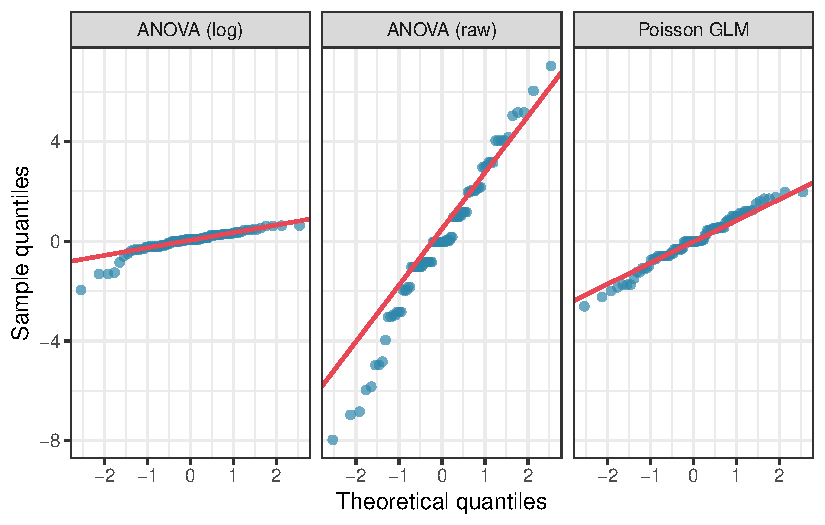
\includegraphics[width=0.9\textwidth,height=\textheight]{04c-when-assumptions-fail_files/figure-pdf/fig-glm-vs-transform-1.pdf}

}

\caption{\label{fig-glm-vs-transform}Comparison of three approaches to
analysing count data: ANOVA on raw counts (top left), ANOVA on
log-transformed counts (top right), and a Poisson GLM (bottom). The
Poisson GLM produces the most appropriate residual structure --- the Q-Q
plot is closest to the diagonal --- because it models the
data-generating process directly rather than approximating it through a
transformation.}

\end{figure}%

\subsection{A Decision Framework}\label{a-decision-framework-1}

\begin{figure}

\centering{


\includegraphics[width=9.8in,height=7.15in]{04c-when-assumptions-fail_files/figure-latex/mermaid-figure-1.png}

}

\caption{\label{fig-assumption-failure-tree}Decision framework for
choosing an analysis strategy when ANOVA assumptions are violated.}

\end{figure}%

\subsection{The Bottom Line}\label{the-bottom-line-1}

The hierarchy of approaches for dealing with assumption violations
reflects an important principle: \textbf{the further a remedy is from
the data-generating process, the less satisfying it is}. A log
transformation is a reasonable approximation for multiplicative data; a
Poisson GLM is the correct model. A rank test avoids distributional
assumptions; a GLM with the right family makes the right assumptions.
Robust ANOVA limits the influence of extreme values; a heavy-tailed
distribution models them explicitly.

For continuous responses with approximately normal residuals and minor
violations, ANOVA and its extensions remain the right tools. For
discrete, bounded, or structurally non-normal responses, the investment
in learning GLMs pays dividends not only in statistical correctness but
in interpretability: a log-odds ratio from a logistic regression, a rate
ratio from a Poisson regression, or a mean ratio from a gamma regression
all have direct biological meaning that a rank difference or a trimmed
mean difference does not.

\chapter{Generalised Linear Mixed Models}\label{sec-chap11}

Chapter \textbf{?@sec-assump} (Section~\ref{sec-glm-intro}) introduced
generalised linear models as the correct framework for non-normal
responses, counts, proportions, binary outcomes, and positive continuous
measurements. Chapter \textbf{?@sec-mem} introduced mixed-effects models
as the correct framework for hierarchical, clustered, and
repeated-measures data. Both extensions were motivated by the same
underlying principle: choose a model whose structure matches the
data-generating process.

Biological data frequently require both extensions simultaneously.
Species abundance counts are non-negative integers (a Poisson or
negative binomial response) and they are collected from plots nested
within sites nested within regions. Disease incidence is a proportion (a
binomial response) but patients are clustered within hospitals. Seed
germination is binary (viable or non viable), but seeds are clustered
within maternal plants, and maternal plants are nested within
populations.

\textbf{Generalised linear mixed models (GLMMs)} combine the
distributional flexibility of GLMs with the random effects structure of
mixed models. They are the natural endpoint of the modelling journey
this book has been tracing, and they are the workhorse of modern
quantitative biology.

\section{The GLMM Framework}\label{the-glmm-framework}

\subsection{The Model}\label{the-model-1}

A GLMM extends the GLM by adding random effects to the linear predictor:

\[g(\mu_{ij}) = \mathbf{x}_{ij}^T \boldsymbol{\beta} +
               \mathbf{z}_{ij}^T \mathbf{b}_j\]

where \(g(\cdot)\) is the link function,
\(\mathbf{x}_{ij}^T \boldsymbol{\beta}\) are the fixed effects,
\(\mathbf{z}_{ij}^T \mathbf{b}_j\) are the random effects
(Section~\ref{sec-matrix-notation}), and
\(\mathbf{b}_j \sim \mathcal{N}(\mathbf{0}, \mathbf{G})\) is the random
effects distribution (Section~\ref{sec-random-effects-distribution}).
The response \(y_{ij}\) follows a distribution from the exponential
family with mean \(\mu_{ij}\).

Three components must be specified:

\begin{enumerate}
\def\labelenumi{\arabic{enumi}.}
\tightlist
\item
  The \textbf{response distribution}: Poisson, negative binomial,
  binomial, gamma, etc.
\item
  The \textbf{link function}: log for counts, logit for proportions,
  identity for Gaussian.
\item
  The \textbf{random effects structure}: which grouping factors to
  include and whether to allow random slopes.
\end{enumerate}

\subsection{Why GLMMs Are Harder Than
LMMs}\label{why-glmms-are-harder-than-lmms}

In a linear mixed model, the random effects can be integrated out
analytically, yielding a closed-form marginal likelihood that is
straightforward to maximise. In a GLMM, the non-linear link function
means this integration has no closed form, then the marginal likelihood
must be approximated numerically. Different packages use different
approximation strategies, each with trade-offs between speed and
accuracy:

\begin{itemize}
\tightlist
\item
  \textbf{Laplace approximation} (\texttt{lme4}, \texttt{glmmTMB}):
  fast, accurate for most designs, but can be unreliable when random
  effect variances are large or when the response is sparse (many zeros,
  very small counts).
\item
  \textbf{Adaptive Gauss-Hermite quadrature} (\texttt{lme4} with
  \texttt{nAGQ\ \textgreater{}\ 1}): more accurate than Laplace,
  particularly for binomial models with few observations per cluster,
  but much slower.
\item
  \textbf{Template Model Builder (TMB)} (\texttt{glmmTMB}): automatic
  differentiation-based Laplace approximation. It is fast, flexible, and
  handles a wide range of distributions and zero-inflation structures.
\end{itemize}

\section{Counts}\label{counts}

\subsection{Poisson GLMM}\label{poisson-glmm}

The Poisson GLMM is the natural model for count responses with a
hierarchical structure. The canonical example in ecology is species
count data: the number of individuals of a species observed at a plot,
where plots are nested within sites and the researcher wants to test the
effect of a habitat treatment.

\begin{Shaded}
\begin{Highlighting}[]
\FunctionTok{library}\NormalTok{(lme4)}
\end{Highlighting}
\end{Shaded}

\begin{verbatim}
#> Loading required package: Matrix
\end{verbatim}

\begin{Shaded}
\begin{Highlighting}[]
\FunctionTok{library}\NormalTok{(glmmTMB)}

\FunctionTok{set.seed}\NormalTok{(}\DecValTok{42}\NormalTok{)}

\NormalTok{n\_sites }\OtherTok{\textless{}{-}} \DecValTok{12}
\NormalTok{n\_plots }\OtherTok{\textless{}{-}} \DecValTok{5}    \CommentTok{\# per site}
\NormalTok{treatment }\OtherTok{\textless{}{-}} \FunctionTok{rep}\NormalTok{(}\FunctionTok{c}\NormalTok{(}\StringTok{"Control"}\NormalTok{, }\StringTok{"Restored"}\NormalTok{), }\AttributeTok{each =}\NormalTok{ n\_sites }\SpecialCharTok{/} \DecValTok{2}\NormalTok{)}

\NormalTok{site\_re }\OtherTok{\textless{}{-}} \FunctionTok{rnorm}\NormalTok{(n\_sites, }\DecValTok{0}\NormalTok{, }\FloatTok{0.6}\NormalTok{)   }\CommentTok{\# site{-}level random effect}
\NormalTok{plot\_data }\OtherTok{\textless{}{-}} \FunctionTok{do.call}\NormalTok{(rbind, }\FunctionTok{lapply}\NormalTok{(}\FunctionTok{seq\_len}\NormalTok{(n\_sites), }\ControlFlowTok{function}\NormalTok{(s) \{}
\NormalTok{  lambda }\OtherTok{\textless{}{-}} \FunctionTok{exp}\NormalTok{(}\FloatTok{2.5} \SpecialCharTok{+} \FloatTok{0.8} \SpecialCharTok{*}\NormalTok{ (treatment[s] }\SpecialCharTok{==} \StringTok{"Restored"}\NormalTok{) }\SpecialCharTok{+}\NormalTok{ site\_re[s])}
  \FunctionTok{data.frame}\NormalTok{(}
    \AttributeTok{count =} \FunctionTok{rpois}\NormalTok{(n\_plots, }\AttributeTok{lambda =}\NormalTok{ lambda),}
    \AttributeTok{treatment =}\NormalTok{ treatment[s],}
    \AttributeTok{site =} \FunctionTok{factor}\NormalTok{(s),}
    \AttributeTok{plot =} \FunctionTok{factor}\NormalTok{(}\FunctionTok{paste0}\NormalTok{(s, }\StringTok{"\_"}\NormalTok{, }\DecValTok{1}\SpecialCharTok{:}\NormalTok{n\_plots))}
\NormalTok{  )}
\NormalTok{\}))}

\NormalTok{plot\_data}\SpecialCharTok{$}\NormalTok{treatment }\OtherTok{\textless{}{-}} \FunctionTok{factor}\NormalTok{(plot\_data}\SpecialCharTok{$}\NormalTok{treatment, }\AttributeTok{levels =} \FunctionTok{c}\NormalTok{(}\StringTok{"Control"}\NormalTok{, }\StringTok{"Restored"}\NormalTok{))}

\CommentTok{\# Poisson GLMM with site as random effect}
\NormalTok{fit\_pois\_glmm }\OtherTok{\textless{}{-}} \FunctionTok{glmer}\NormalTok{(}
\NormalTok{  count }\SpecialCharTok{\textasciitilde{}}\NormalTok{ treatment }\SpecialCharTok{+}\NormalTok{ (}\DecValTok{1} \SpecialCharTok{|}\NormalTok{ site),}
  \AttributeTok{data =}\NormalTok{ plot\_data,}
  \AttributeTok{family =} \FunctionTok{poisson}\NormalTok{(}\AttributeTok{link =} \StringTok{"log"}\NormalTok{)}
\NormalTok{)}
\FunctionTok{summary}\NormalTok{(fit\_pois\_glmm)}
\end{Highlighting}
\end{Shaded}

\begin{verbatim}
#> Generalized linear mixed model fit by maximum likelihood (Laplace
#>   Approximation) [glmerMod]
#>  Family: poisson  ( log )
#> Formula: count ~ treatment + (1 | site)
#>    Data: plot_data
#> 
#>       AIC       BIC    logLik -2*log(L)  df.resid 
#>     437.0     443.3    -215.5     431.0        57 
#> 
#> Scaled residuals: 
#>     Min      1Q  Median      3Q     Max 
#> -2.8959 -0.6454  0.1394  0.7086  2.1713 
#> 
#> Random effects:
#>  Groups Name        Variance Std.Dev.
#>  site   (Intercept) 0.2292   0.4788  
#> Number of obs: 60, groups:  site, 12
#> 
#> Fixed effects:
#>                   Estimate Std. Error z value Pr(>|z|)    
#> (Intercept)         2.7258     0.2012  13.545  < 2e-16 ***
#> treatmentRestored   1.2912     0.2818   4.582  4.6e-06 ***
#> ---
#> Signif. codes:  0 '***' 0.001 '**' 0.01 '*' 0.05 '.' 0.1 ' ' 1
#> 
#> Correlation of Fixed Effects:
#>             (Intr)
#> trtmntRstrd -0.714
\end{verbatim}

\begin{Shaded}
\begin{Highlighting}[]
\CommentTok{\# Exponentiate coefficients to get incidence rate ratios}
\FunctionTok{cat}\NormalTok{(}\StringTok{"}\SpecialCharTok{\textbackslash{}n}\StringTok{Incidence rate ratios (exp of coefficients):}\SpecialCharTok{\textbackslash{}n}\StringTok{"}\NormalTok{)}
\end{Highlighting}
\end{Shaded}

\begin{verbatim}
#> 
#> Incidence rate ratios (exp of coefficients):
\end{verbatim}

\begin{Shaded}
\begin{Highlighting}[]
\FunctionTok{print}\NormalTok{(}\FunctionTok{exp}\NormalTok{(}\FunctionTok{fixef}\NormalTok{(fit\_pois\_glmm)))}
\end{Highlighting}
\end{Shaded}

\begin{verbatim}
#>       (Intercept) treatmentRestored 
#>         15.269302          3.637086
\end{verbatim}

The Poisson GLMM summary output has the same three-section structure as
the linear mixed model summaries seen in Chapter \textbf{?@sec-mem},
with one important difference: the fixed effects are tested with \(z\)
statistics rather than \(t\) statistics, because the Poisson GLMM is
fitted by maximum likelihood and the reference distribution is
asymptotically normal rather than t-distributed.

\textbf{Random effects:} the site-level variance is
\(\hat{\sigma}^2_b = 0.229\) (SD = 0.479). This is the variance in
log-expected counts across sites, after accounting for treatment.
Exponentiated, the standard deviation of 0.479 on the log scale implies
that sites at one standard deviation above the mean have
\(e^{0.479} \approx 1.61\) times the expected count of an average site,
and sites one standard deviation below have \(1 / 1.61 \approx 0.62\)
times the average. The site-level clustering is real and non-trivial and
ignoring it would have produced underestimated standard errors for the
treatment effect.

\textbf{Fixed effects:} the intercept (\(\hat{\beta}_0 = 2.726\)) is the
log expected count in the Control group at an average site.
Exponentiated, \(e^{2.726} \approx 15.3\) individuals per transect in
Control plots which is close to the true simulation mean. The treatment
coefficient (\(\hat{\beta} = 1.291\), \(z = 4.58\), \(p < 0.001\)) is a
log-rate-ratio. Exponentiated, \(e^{1.291} \approx 3.64\): restored
plots have an estimated 3.64 times the bird count of control plots,
after accounting for site-level variation. This is a large and
statistically convincing effect.

The correlation between the intercept and treatment estimates
(\(-0.714\)) is relatively high in absolute value, reflecting the fact
that sites with higher baseline counts (high intercept) tend to show
smaller estimated treatment effects on the log scale which is a
mathematical consequence of the log link rather than a substantive
biological finding.

\textbf{Incidence rate ratios} are the natural summary statistic for
Poisson models. The intercept exponentiated (15.3) gives the expected
count in Control plots; the treatment rate ratio (3.64) gives the
multiplicative factor by which counts increase in Restored plots. A
complete result report would read:

\begin{quote}
Restored plots had significantly higher bird counts than control plots
(\(z = 4.58\), \(p < 0.001\)). The estimated count in control plots was
15.3 individuals per transect (at an average site); the incidence rate
ratio for restoration was 3.64 (95\% CI: \ldots), indicating that
restored plots had approximately 3.6 times the count of control plots
after accounting for site-level variation
(\(\hat{\sigma}_{\text{site}} = 0.479\)).
\end{quote}

\subsection{Checking for
Overdispersion}\label{checking-for-overdispersion}

The Poisson distribution assumes that the variance equals the mean. In
practice, ecological count data are almost always overdispersed meaning
that the variance exceeds the mean, due to aggregation, unmodelled
heterogeneity, or excess zeros. Overdispersion inflates standard errors
and inflates the false positive rate if ignored.

\begin{Shaded}
\begin{Highlighting}[]
\CommentTok{\# Overdispersion check: ratio of residual deviance to df}
\CommentTok{\# Values substantially above 1 indicate overdispersion}
\NormalTok{overdisp\_ratio }\OtherTok{\textless{}{-}} \FunctionTok{deviance}\NormalTok{(fit\_pois\_glmm) }\SpecialCharTok{/} \FunctionTok{df.residual}\NormalTok{(fit\_pois\_glmm)}
\FunctionTok{cat}\NormalTok{(}\StringTok{"Overdispersion ratio:"}\NormalTok{, }\FunctionTok{round}\NormalTok{(overdisp\_ratio, }\DecValTok{3}\NormalTok{), }\StringTok{"}\SpecialCharTok{\textbackslash{}n}\StringTok{"}\NormalTok{)}
\end{Highlighting}
\end{Shaded}

\begin{verbatim}
#> Overdispersion ratio: 1.161
\end{verbatim}

\begin{Shaded}
\begin{Highlighting}[]
\CommentTok{\# Simulation{-}based overdispersion test via DHARMa}
\CommentTok{\# install.packages("DHARMa") if needed}
\FunctionTok{library}\NormalTok{(DHARMa)}
\end{Highlighting}
\end{Shaded}

\begin{verbatim}
#> This is DHARMa 0.5.0. For overview type '?DHARMa'. For recent changes, type news(package = 'DHARMa') 
#> 
#> Note that the default setting in simulateResiduals was changed to conditional simulations since version 0.5.0. This is likely to change residual calculations for all hierarchical (in particular random effect) models. If you want to switch back to the old package version defaults, please use the argument simulateREs = "user-specified" in simulateResiduals(). For more details, see ?simulateREsiduals.
\end{verbatim}

\begin{verbatim}
#> 
#> Attaching package: 'DHARMa'
\end{verbatim}

\begin{verbatim}
#> The following object is masked from 'package:lme4':
#> 
#>     getData
\end{verbatim}

\begin{Shaded}
\begin{Highlighting}[]
\NormalTok{sim\_res }\OtherTok{\textless{}{-}} \FunctionTok{simulateResiduals}\NormalTok{(fit\_pois\_glmm, }\AttributeTok{n =} \DecValTok{1000}\NormalTok{)}
\FunctionTok{testDispersion}\NormalTok{(sim\_res)}
\end{Highlighting}
\end{Shaded}

\begin{center}
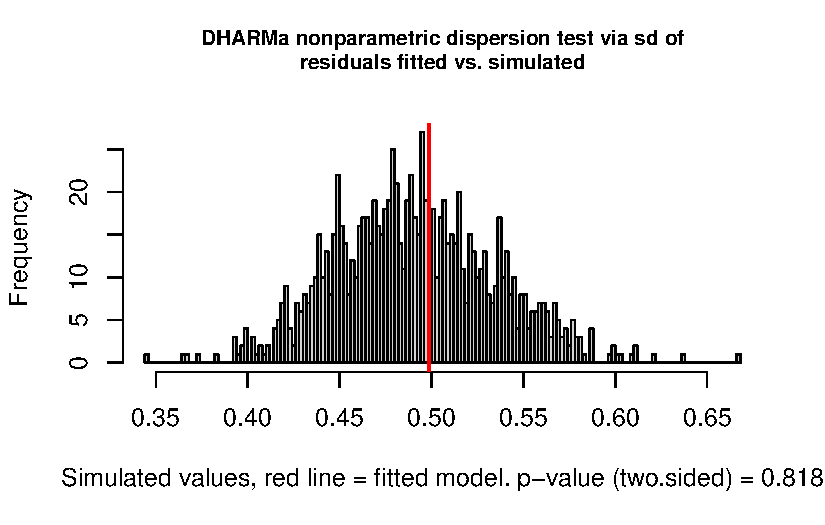
\includegraphics[width=0.9\textwidth,height=\textheight]{04d-glmm_files/figure-pdf/overdispersion-check-1.pdf}
\end{center}

\begin{verbatim}
#> 
#>  DHARMa nonparametric dispersion test via sd of residuals fitted vs.
#>  simulated
#> 
#> data:  simulationOutput
#> dispersion = 1.0155, p-value = 0.818
#> alternative hypothesis: two.sided
\end{verbatim}

\begin{Shaded}
\begin{Highlighting}[]
\FunctionTok{plot}\NormalTok{(sim\_res)}
\end{Highlighting}
\end{Shaded}

\begin{center}
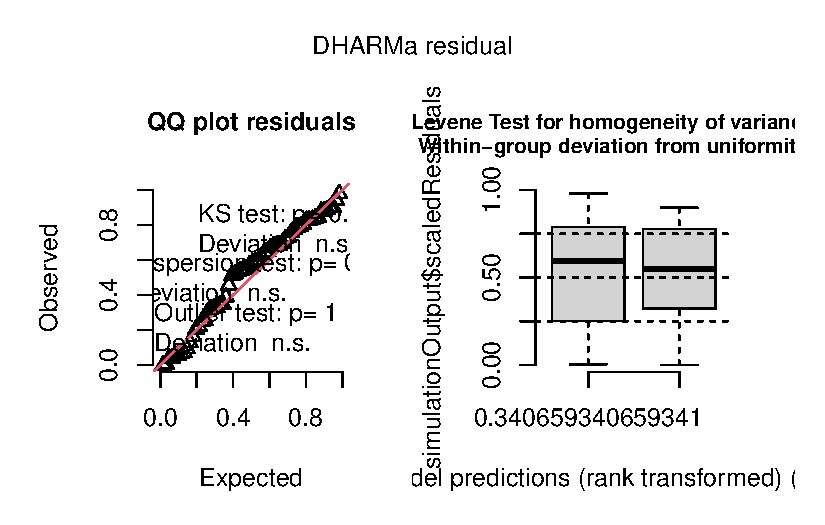
\includegraphics[width=0.9\textwidth,height=\textheight]{04d-glmm_files/figure-pdf/overdispersion-check-2.pdf}
\end{center}

\texttt{DHARMa} \citep{Hartig2022} is the recommended diagnostic package
for GLMMs. Rather than computing analytical residuals (which do not have
a standard distribution for GLMMs), it simulates data from the fitted
model and compares the observed data to the simulated distribution. The
resulting quantile residuals are uniformly distributed under a correctly
specified model, making them interpretable in the same way as normal Q-Q
plots.

Both the analytical and simulation-based diagnostics confirm that the
Poisson model is adequate for these data and overdispersion is not a
concern.

The analytical overdispersion ratio, residual deviance divided by
residual degrees of freedom, is 1.161, modestly above 1 but well within
the range expected from sampling variation for a correctly specified
Poisson model. A ratio of this magnitude does not warrant switching to a
negative binomial.

The DHARMa dispersion test corroborates this. The test statistic is
1.016 (\(p = 0.818\)), meaning the observed dispersion in the data is
indistinguishable from the dispersion expected under the fitted Poisson
model. The histogram in the dispersion test plot shows the distribution
of dispersion statistics from 1000 simulated datasets generated under
the fitted model; the red vertical line marks the observed value, which
sits comfortably in the centre of the simulated distribution, exactly
where it should be under a well-fitting model.

The DHARMa QQ plot reinforces this conclusion. The quantile residuals
lie closely along the diagonal (KS test \(p = 0.267\), deviation
non-significant), the dispersion test is non-significant, and the
outlier test returns \(p = 1\) --- no observations are flagged as
outliers. The residuals vs fitted boxplot on the right shows
approximately uniform spread across the range of model predictions, with
the Levene test and within-group uniformity test both non-significant.
Taken together, the diagnostics present a consistent and reassuring
picture: the Poisson GLMM with a random intercept for site provides an
adequate description of these count data, and there is no evidence that
a more complex model, negative binomial, zero-inflated, or otherwise, is
needed.

\subsection{Negative Binomial GLMM}\label{negative-binomial-glmm}

When overdispersion is detected, the next coherent step is to replace
the Poisson with a negative binomial distribution, which adds a
dispersion parameter \(\theta\) that allows the variance to exceed the
mean:

\[\text{Var}(y) = \mu + \frac{\mu^2}{\theta}\]

\begin{Shaded}
\begin{Highlighting}[]
\CommentTok{\# Negative binomial GLMM via glmmTMB}
\CommentTok{\# (lme4 does not support negative binomial directly)}
\NormalTok{fit\_nb\_glmm }\OtherTok{\textless{}{-}} \FunctionTok{glmmTMB}\NormalTok{(}
\NormalTok{  count }\SpecialCharTok{\textasciitilde{}}\NormalTok{ treatment }\SpecialCharTok{+}\NormalTok{ (}\DecValTok{1} \SpecialCharTok{|}\NormalTok{ site),}
  \AttributeTok{data   =}\NormalTok{ plot\_data,}
  \AttributeTok{family =} \FunctionTok{nbinom2}\NormalTok{(}\AttributeTok{link =} \StringTok{"log"}\NormalTok{)}
\NormalTok{)}
\FunctionTok{summary}\NormalTok{(fit\_nb\_glmm)}
\end{Highlighting}
\end{Shaded}

\begin{verbatim}
#>  Family: nbinom2  ( log )
#> Formula:          count ~ treatment + (1 | site)
#> Data: plot_data
#> 
#>       AIC       BIC    logLik -2*log(L)  df.resid 
#>     439.0     447.4    -215.5     431.0        56 
#> 
#> Random effects:
#> 
#> Conditional model:
#>  Groups Name        Variance Std.Dev.
#>  site   (Intercept) 0.2292   0.4788  
#> Number of obs: 60, groups:  site, 12
#> 
#> Dispersion parameter for nbinom2 family (): 6.01e+07 
#> 
#> Conditional model:
#>                   Estimate Std. Error z value Pr(>|z|)    
#> (Intercept)         2.7258     0.2013  13.542  < 2e-16 ***
#> treatmentRestored   1.2912     0.2818   4.582 4.61e-06 ***
#> ---
#> Signif. codes:  0 '***' 0.001 '**' 0.01 '*' 0.05 '.' 0.1 ' ' 1
\end{verbatim}

\begin{Shaded}
\begin{Highlighting}[]
\CommentTok{\# Compare Poisson vs negative binomial via AIC}
\FunctionTok{AIC}\NormalTok{(fit\_pois\_glmm, fit\_nb\_glmm)}
\end{Highlighting}
\end{Shaded}

\begin{verbatim}
#>               df      AIC
#> fit_pois_glmm  3 437.0404
#> fit_nb_glmm    4 439.0404
\end{verbatim}

\begin{Shaded}
\begin{Highlighting}[]
\CommentTok{\# DHARMa diagnostics for negative binomial model}
\NormalTok{sim\_res\_nb }\OtherTok{\textless{}{-}} \FunctionTok{simulateResiduals}\NormalTok{(fit\_nb\_glmm, }\AttributeTok{n =} \DecValTok{1000}\NormalTok{)}
\FunctionTok{plot}\NormalTok{(sim\_res\_nb)}
\end{Highlighting}
\end{Shaded}

\begin{center}
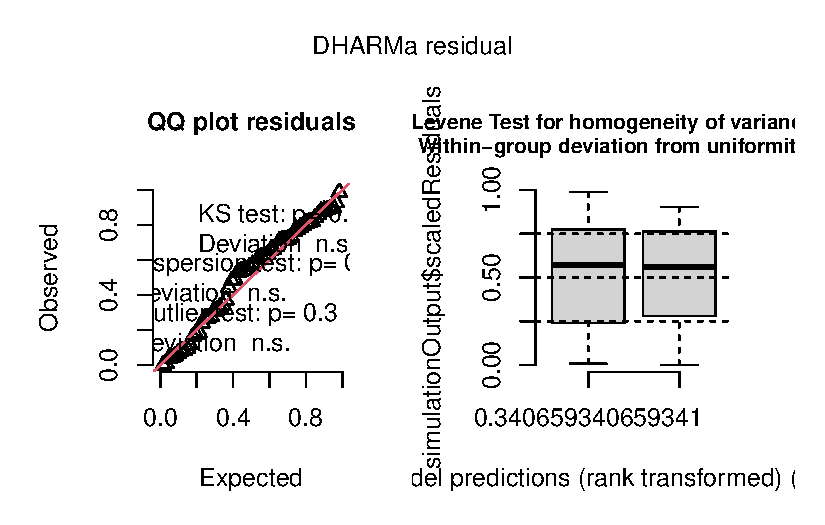
\includegraphics[width=0.9\textwidth,height=\textheight]{04d-glmm_files/figure-pdf/nb-glmm-1.pdf}
\end{center}

The negative binomial model confirms what the overdispersion diagnostics
already suggested: the Poisson model is the correct choice for these
data and the additional complexity of the negative binomial is not
warranted.

The most telling indicator is the estimated dispersion parameter
\(\hat{\theta} = 6.01 \times 10^7\), an astronomically large value.
Recall that the negative binomial variance is \(\mu + \mu^2/\theta\): as
\(\theta \to \infty\), the \(\mu^2/\theta\) term vanishes and the
negative binomial collapses exactly to a Poisson. The model is telling
us, unambiguously, that there is no extra-Poisson dispersion to account
for. The fixed effect estimates and the site-level variance are
identical to four decimal places between the two models
(\(\hat{\beta}_{\text{treatment}} = 1.291\),
\(\hat{\sigma}_{\text{site}} = 0.479\)), confirming that the Poisson and
negative binomial fits are numerically equivalent here.

The AIC comparison makes the model selection decision explicit. The
Poisson model (AIC = 437.0) is preferred over the negative binomial (AIC
= 439.0) --- a difference of 2 AIC units in favour of the simpler model,
which is exactly the penalty for the one additional parameter
(\(\theta\)) that the negative binomial estimates but does not need.
When the simpler model fits equally well, parsimony favours it.

The DHARMa diagnostics for the negative binomial model (QQ plot: KS
\(p = 0.398\); dispersion test: \(p = 0.856\); outlier test:
\(p = 0.3\)) are similarly clean and essentially identical to those of
the Poisson model. Both the Levene test and the within-group uniformity
test are non-significant, and the residuals vs fitted boxplot shows
uniform spread across the range of predictions. The negative binomial
model fits the data no better than the Poisson, it simply uses an extra
parameter to arrive at the same conclusion.

The practical lesson is important: do not fit a negative binomial model
by default for count data. Check the overdispersion ratio and the DHARMa
dispersion test first. If neither flags a problem, the Poisson model is
both correct and more parsimonious. Reserve the negative binomial for
situations where overdispersion is genuinely present, which, in ecology
and biology, is more often than not, but should be confirmed rather than
assumed.

\subsection{Zero-Inflated Models: A
Note}\label{zero-inflated-models-a-note}

Ecological count data sometimes contain more zeros than any standard
count distribution predicts, a phenomenon called \textbf{zero
inflation}. Zero inflation arises when two distinct biological processes
generate zeros: structural zeros (the species is genuinely absent from
this site, it could never be counted there) and sampling zeros (the
species is present but was not detected on this occasion). Mixing these
two processes in a single Poisson or negative binomial model produces
poor fit and biased estimates.

\texttt{glmmTMB} handles zero inflation elegantly through the
\texttt{ziformula} argument, which specifies a separate model for the
probability of structural zeros. However, zero-inflated models should
only be fitted when there is genuine biological reason to expect
structural zeros, and the DHARMa zero-inflation test on the simpler
model should confirm the problem before adding the extra complexity.

The worked example in Section 11.7 demonstrates a zero-inflated negative
binomial GLMM in a context where zero inflation is biologically
motivated and statistically necessary, a species abundance survey where
many sites are genuinely unoccupied.

\section{Proportions}\label{proportions}

\subsection{Binomial GLMM}\label{binomial-glmm}

When the response is a proportion like the fraction of seeds
germinating, the proportion of patients responding, or the fraction of
eggs hatching, and observations are clustered, the binomial GLMM is the
correct model.

\begin{Shaded}
\begin{Highlighting}[]
\FunctionTok{set.seed}\NormalTok{(}\DecValTok{42}\NormalTok{)}

\NormalTok{n\_hospitals }\OtherTok{\textless{}{-}} \DecValTok{10}
\NormalTok{n\_patients }\OtherTok{\textless{}{-}} \DecValTok{15}  \CommentTok{\# per hospital}

\NormalTok{hospital\_re }\OtherTok{\textless{}{-}} \FunctionTok{rnorm}\NormalTok{(n\_hospitals, }\DecValTok{0}\NormalTok{, }\FloatTok{0.8}\NormalTok{)}

\NormalTok{df\_binom }\OtherTok{\textless{}{-}} \FunctionTok{do.call}\NormalTok{(rbind, }\FunctionTok{lapply}\NormalTok{(}\FunctionTok{seq\_len}\NormalTok{(n\_hospitals), }\ControlFlowTok{function}\NormalTok{(h) \{}
\NormalTok{  treatment }\OtherTok{\textless{}{-}} \FunctionTok{rep}\NormalTok{(}\FunctionTok{c}\NormalTok{(}\StringTok{"Control"}\NormalTok{, }\StringTok{"Treatment"}\NormalTok{),}
                   \AttributeTok{length.out =}\NormalTok{ n\_patients)}
\NormalTok{  log\_odds  }\OtherTok{\textless{}{-}} \SpecialCharTok{{-}}\FloatTok{0.5} \SpecialCharTok{+} \FloatTok{1.2} \SpecialCharTok{*}\NormalTok{ (treatment }\SpecialCharTok{==} \StringTok{"Treatment"}\NormalTok{) }\SpecialCharTok{+}
\NormalTok{               hospital\_re[h]}
\NormalTok{  prob      }\OtherTok{\textless{}{-}} \FunctionTok{plogis}\NormalTok{(log\_odds)}
  \FunctionTok{data.frame}\NormalTok{(}
    \AttributeTok{response  =} \FunctionTok{rbinom}\NormalTok{(n\_patients, }\AttributeTok{size =} \DecValTok{1}\NormalTok{, }\AttributeTok{prob =}\NormalTok{ prob),}
    \AttributeTok{treatment =} \FunctionTok{factor}\NormalTok{(treatment,}
                       \AttributeTok{levels =} \FunctionTok{c}\NormalTok{(}\StringTok{"Control"}\NormalTok{, }\StringTok{"Treatment"}\NormalTok{)),}
    \AttributeTok{hospital  =} \FunctionTok{factor}\NormalTok{(h)}
\NormalTok{  )}
\NormalTok{\}))}

\CommentTok{\# Binomial GLMM with logit link}
\NormalTok{fit\_binom\_glmm }\OtherTok{\textless{}{-}} \FunctionTok{glmer}\NormalTok{(}
\NormalTok{  response }\SpecialCharTok{\textasciitilde{}}\NormalTok{ treatment }\SpecialCharTok{+}\NormalTok{ (}\DecValTok{1} \SpecialCharTok{|}\NormalTok{ hospital),}
  \AttributeTok{data   =}\NormalTok{ df\_binom,}
  \AttributeTok{family =} \FunctionTok{binomial}\NormalTok{(}\AttributeTok{link =} \StringTok{"logit"}\NormalTok{)}
\NormalTok{)}
\FunctionTok{summary}\NormalTok{(fit\_binom\_glmm)}
\end{Highlighting}
\end{Shaded}

\begin{verbatim}
#> Generalized linear mixed model fit by maximum likelihood (Laplace
#>   Approximation) [glmerMod]
#>  Family: binomial  ( logit )
#> Formula: response ~ treatment + (1 | hospital)
#>    Data: df_binom
#> 
#>       AIC       BIC    logLik -2*log(L)  df.resid 
#>     193.7     202.7     -93.8     187.7       147 
#> 
#> Scaled residuals: 
#>     Min      1Q  Median      3Q     Max 
#> -2.3962 -0.9464  0.4173  0.6677  1.3708 
#> 
#> Random effects:
#>  Groups   Name        Variance Std.Dev.
#>  hospital (Intercept) 0.45     0.6709  
#> Number of obs: 150, groups:  hospital, 10
#> 
#> Fixed effects:
#>                    Estimate Std. Error z value Pr(>|z|)  
#> (Intercept)          0.1694     0.3175   0.533   0.5937  
#> treatmentTreatment   0.9179     0.3687   2.490   0.0128 *
#> ---
#> Signif. codes:  0 '***' 0.001 '**' 0.01 '*' 0.05 '.' 0.1 ' ' 1
#> 
#> Correlation of Fixed Effects:
#>             (Intr)
#> trtmntTrtmn -0.468
\end{verbatim}

\begin{Shaded}
\begin{Highlighting}[]
\CommentTok{\# Exponentiate to get odds ratios}
\FunctionTok{cat}\NormalTok{(}\StringTok{"}\SpecialCharTok{\textbackslash{}n}\StringTok{Odds ratios:}\SpecialCharTok{\textbackslash{}n}\StringTok{"}\NormalTok{)}
\end{Highlighting}
\end{Shaded}

\begin{verbatim}
#> 
#> Odds ratios:
\end{verbatim}

\begin{Shaded}
\begin{Highlighting}[]
\FunctionTok{print}\NormalTok{(}\FunctionTok{exp}\NormalTok{(}\FunctionTok{fixef}\NormalTok{(fit\_binom\_glmm)))}
\end{Highlighting}
\end{Shaded}

\begin{verbatim}
#>        (Intercept) treatmentTreatment 
#>           1.184541           2.503988
\end{verbatim}

\begin{Shaded}
\begin{Highlighting}[]
\CommentTok{\# Confidence intervals on odds ratio scale}
\FunctionTok{cat}\NormalTok{(}\StringTok{"}\SpecialCharTok{\textbackslash{}n}\StringTok{95\% CI for odds ratios:}\SpecialCharTok{\textbackslash{}n}\StringTok{"}\NormalTok{)}
\end{Highlighting}
\end{Shaded}

\begin{verbatim}
#> 
#> 95% CI for odds ratios:
\end{verbatim}

\begin{Shaded}
\begin{Highlighting}[]
\FunctionTok{print}\NormalTok{(}\FunctionTok{exp}\NormalTok{(}\FunctionTok{confint}\NormalTok{(fit\_binom\_glmm, }\AttributeTok{method =} \StringTok{"Wald"}\NormalTok{)))}
\end{Highlighting}
\end{Shaded}

\begin{verbatim}
#>                        2.5 %   97.5 %
#> .sig01                    NA       NA
#> (Intercept)        0.6357912 2.206915
#> treatmentTreatment 1.2156859 5.157544
\end{verbatim}

The binomial GLMM output follows the same three-section structure as the
Poisson model, with coefficients now on the logit scale and interpreted
as log-odds ratios.

\textbf{Random effects:} the hospital-level variance is
\(\hat{\sigma}^2_b = 0.450\) (SD = 0.671). This is the variance in
log-odds of response across hospitals, after accounting for treatment.
On the probability scale, a hospital one standard deviation above
average has a baseline response probability of
\(\text{plogis}(0.169 + 0.671) = 0.699\), while a hospital one standard
deviation below average has \(\text{plogis}(0.169 - 0.671) = 0.376\).
The ICC for a binomial GLMM on the latent scale is
\(0.450 / (0.450 + \pi^2/3) = 0.120\), meaning approximately 12\% of the
total variation in the latent response propensity is attributable to
hospital-level clustering. This is modest but non-negligible: ignoring
the hospital random effect would have produced slightly underestimated
standard errors for the treatment comparison.

\textbf{Fixed effects:} the intercept (\(\hat{\beta}_0 = 0.169\),
\(z = 0.533\), \(p = 0.594\)) is the log-odds of a positive response in
the Control group at an average hospital. Its non-significance simply
means the baseline response probability is not significantly different
from 50\% which is an intercept test that is rarely of scientific
interest. The treatment coefficient (\(\hat{\beta} = 0.918\),
\(z = 2.49\), \(p = 0.013\)) is the log-odds ratio for treatment vs
control. Exponentiated, \(e^{0.918} = 2.50\): the odds of a positive
response are 2.5 times higher in the Treatment group than in the Control
group, after accounting for hospital-level clustering. The 95\% Wald
confidence interval for this odds ratio is \([1.22, 5.16]\), comfortably
excluding 1 and confirming that the treatment effect is real.

The correlation between the intercept and treatment estimates
(\(-0.468\)) reflects the design balance: with 7-8 patients per
treatment per hospital, the two coefficient estimates share information
about each hospital's baseline, producing moderate negative correlation.
This is expected and does not indicate any modelling problem.

\textbf{Back-transformed predictions} make the result immediately
interpretable. The Control group response probability at an average
hospital is \(\text{plogis}(0.169) = 0.542\), about 54\%. The Treatment
group probability is \(\text{plogis}(0.169 + 0.918) = 0.748\), about
75\%. The treatment increases the probability of a positive response by
approximately 21 percentage points at an average hospital.

A complete result report reads:

\begin{quote}
The effect of treatment on binary response was analysed using a binomial
GLMM with a logit link, with treatment as a fixed effect and a random
intercept for hospital. Treatment had a significant positive effect on
response probability (\(z = 2.49\), \(p = 0.013\); OR = 2.50, 95\% CI:
\([1.22, 5.16]\)). The estimated response probability was 54.2\% in the
Control group and 74.8\% in the Treatment group at an average hospital.
Hospital-level variance was \(\hat{\sigma}^2_b = 0.450\), indicating
modest clustering of outcomes within hospitals that was accounted for in
the analysis.
\end{quote}

\subsection{Overdispersion in Binomial Models:
Beta-Binomial}\label{overdispersion-in-binomial-models-beta-binomial}

Binary responses (0/1) cannot be overdispersed by definition: a
Bernoulli trial has variance \(p(1-p)\) with no free parameter. But when
the response is a proportion of successes out of \(n\) trials (e.g.~7
out of 20 seeds germinating), overdispersion is possible and common. The
beta-binomial distribution handles this:

\begin{Shaded}
\begin{Highlighting}[]
\FunctionTok{set.seed}\NormalTok{(}\DecValTok{42}\NormalTok{)}

\NormalTok{n\_plants }\OtherTok{\textless{}{-}} \DecValTok{30}
\NormalTok{n\_seeds }\OtherTok{\textless{}{-}} \DecValTok{20}
\NormalTok{treatment }\OtherTok{\textless{}{-}} \FunctionTok{factor}\NormalTok{(}\FunctionTok{rep}\NormalTok{(}\FunctionTok{c}\NormalTok{(}\StringTok{"Control"}\NormalTok{, }\StringTok{"Treated"}\NormalTok{), }\AttributeTok{each =}\NormalTok{ n\_plants }\SpecialCharTok{/} \DecValTok{2}\NormalTok{))}

\CommentTok{\# Simulate beta{-}binomial data manually:}
\CommentTok{\# Step 1: draw plant{-}level probabilities from a Beta distribution}
\CommentTok{\# Step 2: draw seed counts from a Binomial given those probabilities}
\CommentTok{\# This two{-}step process is exactly what the beta{-}binomial distribution models}

\CommentTok{\# Beta parameters derived from mean (mu) and dispersion (theta):}
\CommentTok{\# shape1 = mu * theta, shape2 = (1 {-} mu) * theta}
\NormalTok{mu\_control }\OtherTok{\textless{}{-}} \FloatTok{0.3}
\NormalTok{mu\_treated }\OtherTok{\textless{}{-}} \FloatTok{0.6}
\NormalTok{theta      }\OtherTok{\textless{}{-}} \DecValTok{5}    \CommentTok{\# smaller theta = more overdispersion}

\NormalTok{p\_control }\OtherTok{\textless{}{-}} \FunctionTok{rbeta}\NormalTok{(n\_plants }\SpecialCharTok{/} \DecValTok{2}\NormalTok{,}
                   \AttributeTok{shape1 =}\NormalTok{ mu\_control }\SpecialCharTok{*}\NormalTok{ theta,}
                   \AttributeTok{shape2 =}\NormalTok{ (}\DecValTok{1} \SpecialCharTok{{-}}\NormalTok{ mu\_control) }\SpecialCharTok{*}\NormalTok{ theta)}

\NormalTok{p\_treated }\OtherTok{\textless{}{-}} \FunctionTok{rbeta}\NormalTok{(n\_plants }\SpecialCharTok{/} \DecValTok{2}\NormalTok{,}
                   \AttributeTok{shape1 =}\NormalTok{ mu\_treated }\SpecialCharTok{*}\NormalTok{ theta,}
                   \AttributeTok{shape2 =}\NormalTok{ (}\DecValTok{1} \SpecialCharTok{{-}}\NormalTok{ mu\_treated) }\SpecialCharTok{*}\NormalTok{ theta)}

\NormalTok{n\_germ }\OtherTok{\textless{}{-}} \FunctionTok{c}\NormalTok{(}
  \FunctionTok{rbinom}\NormalTok{(n\_plants }\SpecialCharTok{/} \DecValTok{2}\NormalTok{, }\AttributeTok{size =}\NormalTok{ n\_seeds, }\AttributeTok{prob =}\NormalTok{ p\_control),}
  \FunctionTok{rbinom}\NormalTok{(n\_plants }\SpecialCharTok{/} \DecValTok{2}\NormalTok{, }\AttributeTok{size =}\NormalTok{ n\_seeds, }\AttributeTok{prob =}\NormalTok{ p\_treated)}
\NormalTok{)}

\NormalTok{df\_bb }\OtherTok{\textless{}{-}} \FunctionTok{data.frame}\NormalTok{(}
  \AttributeTok{n\_germ    =}\NormalTok{ n\_germ,}
  \AttributeTok{n\_fail    =}\NormalTok{ n\_seeds }\SpecialCharTok{{-}}\NormalTok{ n\_germ,}
  \AttributeTok{treatment =}\NormalTok{ treatment}
\NormalTok{)}

\CommentTok{\# Fit beta{-}binomial GLMM via glmmTMB}
\NormalTok{fit\_bb }\OtherTok{\textless{}{-}}\NormalTok{ glmmTMB}\SpecialCharTok{::}\FunctionTok{glmmTMB}\NormalTok{(}
  \FunctionTok{cbind}\NormalTok{(n\_germ, n\_fail) }\SpecialCharTok{\textasciitilde{}}\NormalTok{ treatment,}
  \AttributeTok{data   =}\NormalTok{ df\_bb,}
  \AttributeTok{family =}\NormalTok{ glmmTMB}\SpecialCharTok{::}\FunctionTok{betabinomial}\NormalTok{(}\AttributeTok{link =} \StringTok{"logit"}\NormalTok{)}
\NormalTok{)}
\FunctionTok{summary}\NormalTok{(fit\_bb)}
\end{Highlighting}
\end{Shaded}

\begin{verbatim}
#>  Family: betabinomial  ( logit )
#> Formula:          cbind(n_germ, n_fail) ~ treatment
#> Data: df_bb
#> 
#>       AIC       BIC    logLik -2*log(L)  df.resid 
#>     182.5     186.7     -88.2     176.5        27 
#> 
#> 
#> Dispersion parameter for betabinomial family (): 2.74 
#> 
#> Conditional model:
#>                  Estimate Std. Error z value Pr(>|z|)  
#> (Intercept)       -0.4765     0.2863  -1.664   0.0961 .
#> treatmentTreated   1.0375     0.4107   2.526   0.0115 *
#> ---
#> Signif. codes:  0 '***' 0.001 '**' 0.01 '*' 0.05 '.' 0.1 ' ' 1
\end{verbatim}

\begin{Shaded}
\begin{Highlighting}[]
\CommentTok{\# Compare to standard binomial to confirm overdispersion}
\NormalTok{fit\_binom\_bb }\OtherTok{\textless{}{-}}\NormalTok{ glmmTMB}\SpecialCharTok{::}\FunctionTok{glmmTMB}\NormalTok{(}
  \FunctionTok{cbind}\NormalTok{(n\_germ, n\_fail) }\SpecialCharTok{\textasciitilde{}}\NormalTok{ treatment,}
  \AttributeTok{data   =}\NormalTok{ df\_bb,}
  \AttributeTok{family =} \FunctionTok{binomial}\NormalTok{(}\AttributeTok{link =} \StringTok{"logit"}\NormalTok{)}
\NormalTok{)}

\FunctionTok{cat}\NormalTok{(}\StringTok{"AIC binomial:"}\NormalTok{, }\FunctionTok{AIC}\NormalTok{(fit\_binom\_bb), }\StringTok{"}\SpecialCharTok{\textbackslash{}n}\StringTok{"}\NormalTok{)}
\end{Highlighting}
\end{Shaded}

\begin{verbatim}
#> AIC binomial: 295.9792
\end{verbatim}

\begin{Shaded}
\begin{Highlighting}[]
\FunctionTok{cat}\NormalTok{(}\StringTok{"AIC beta{-}binomial:"}\NormalTok{, }\FunctionTok{AIC}\NormalTok{(fit\_bb), }\StringTok{"}\SpecialCharTok{\textbackslash{}n}\StringTok{"}\NormalTok{)}
\end{Highlighting}
\end{Shaded}

\begin{verbatim}
#> AIC beta-binomial: 182.4932
\end{verbatim}

The results make a compelling case for the beta-binomial model and a
illustrate of why standard binomial models fail with overdispersed
proportion data.

The AIC comparison is decisive: the beta-binomial model (AIC = 182.5) is
dramatically preferred over the standard binomial (AIC = 295.9), a
difference of \(\Delta\)AIC = 113.5. This is an enormous improvement,
differences above 10 are already considered very strong evidence in
favour of the better model, and a difference of 113 units reflects a
fundamental failure of the binomial model to capture the true variance
structure of the data. The standard binomial model is forcing the
variance to follow \(p(1-p)/n\) exactly, when the actual plant-to-plant
variation in germination probability, driven by differences in seed
quality, maternal effects, and microenvironmental variation, produces
far more spread than this constraint allows.

The estimated dispersion parameter \(\hat{\phi} = 2.74\) quantifies the
overdispersion directly. In the beta-binomial parameterisation used by
\texttt{glmmTMB}, larger values of \(\phi\) indicate less overdispersion
(the distribution converges to binomial as \(\phi \to \infty\)). A value
of 2.74 indicates substantial overdispersion indicating that the
germination probabilities vary considerably among plants within each
treatment group, consistent with the two-step simulation process:
plant-level probabilities drawn from a Beta distribution, then counts
drawn from a Binomial given those probabilities.

The fixed effect for treatment (\(\hat{\beta} = 1.038\), \(z = 2.53\),
\(p = 0.012\)) is a log-odds ratio. Exponentiated, \(e^{1.038} = 2.82\):
the odds of a seed germinating are 2.82 times higher in the Treated
group than in the Control group. The intercept
(\(\hat{\beta}_0 = -0.477\), \(p = 0.096\)) gives the log-odds of
germination in the Control group at an average plant:
\(\text{plogis}(-0.477) = 0.383\), a germination probability of about
38\%, close to the true simulation value of 0.30. The Treated group
probability is \(\text{plogis}(-0.477 + 1.038) = 0.637\), approximately
64\%, again close to the true value of 0.60.

The practical lesson is direct: when proportion data show more
plant-to-plant, subject-to-subject, or unit-to-unit variation in the
underlying probability than the binomial distribution predicts, the
beta-binomial is the correct model. Using a standard binomial in this
situation does not just produce slightly wrong standard errors, the AIC
difference of 113 units shows it produces catastrophically wrong
standard errors, and any inference drawn from it would be severely
misleading. The beta-binomial adds only one parameter (\(\phi\)) over
the standard binomial, and the return on that investment here is
enormous.

\section{Other Cases}\label{other-cases}

\subsection{Gamma GLMM for Positive Continuous
Responses}\label{gamma-glmm-for-positive-continuous-responses}

When the response is strictly positive and continuous like for biomass,
enzyme activity, reaction time, body mass, and the coefficient of
variation is approximately constant across groups, a gamma GLMM with a
log link is often more appropriate than a log-transformed Gaussian
model:

\begin{Shaded}
\begin{Highlighting}[]
\FunctionTok{set.seed}\NormalTok{(}\DecValTok{42}\NormalTok{)}

\NormalTok{n\_sites  }\OtherTok{\textless{}{-}} \DecValTok{8}
\NormalTok{n\_obs }\OtherTok{\textless{}{-}} \DecValTok{10}

\NormalTok{site\_re  }\OtherTok{\textless{}{-}} \FunctionTok{rnorm}\NormalTok{(n\_sites, }\DecValTok{0}\NormalTok{, }\FloatTok{0.4}\NormalTok{)}
\NormalTok{treatment }\OtherTok{\textless{}{-}} \FunctionTok{rep}\NormalTok{(}\FunctionTok{c}\NormalTok{(}\StringTok{"Control"}\NormalTok{, }\StringTok{"Treatment"}\NormalTok{), }\AttributeTok{each =}\NormalTok{ n\_sites }\SpecialCharTok{/} \DecValTok{2}\NormalTok{)}

\NormalTok{df\_gamma }\OtherTok{\textless{}{-}} \FunctionTok{do.call}\NormalTok{(rbind, }\FunctionTok{lapply}\NormalTok{(}\FunctionTok{seq\_len}\NormalTok{(n\_sites), }\ControlFlowTok{function}\NormalTok{(s) \{}
\NormalTok{  mu }\OtherTok{\textless{}{-}} \FunctionTok{exp}\NormalTok{(}\FloatTok{2.0} \SpecialCharTok{+} \FloatTok{0.5} \SpecialCharTok{*}\NormalTok{ (treatment[s] }\SpecialCharTok{==} \StringTok{"Treatment"}\NormalTok{) }\SpecialCharTok{+}\NormalTok{ site\_re[s])}
  \FunctionTok{data.frame}\NormalTok{(}
    \AttributeTok{biomass =} \FunctionTok{rgamma}\NormalTok{(n\_obs, }\AttributeTok{shape =} \DecValTok{4}\NormalTok{, }\AttributeTok{rate =} \DecValTok{4} \SpecialCharTok{/}\NormalTok{ mu),}
    \AttributeTok{treatment =}\NormalTok{ treatment[s],}
    \AttributeTok{site =} \FunctionTok{factor}\NormalTok{(s)}
\NormalTok{  )}
\NormalTok{\}))}
\NormalTok{df\_gamma}\SpecialCharTok{$}\NormalTok{treatment }\OtherTok{\textless{}{-}} \FunctionTok{factor}\NormalTok{(df\_gamma}\SpecialCharTok{$}\NormalTok{treatment,}
                              \AttributeTok{levels =} \FunctionTok{c}\NormalTok{(}\StringTok{"Control"}\NormalTok{, }\StringTok{"Treatment"}\NormalTok{))}

\NormalTok{fit\_gamma\_glmm }\OtherTok{\textless{}{-}} \FunctionTok{glmmTMB}\NormalTok{(}
\NormalTok{  biomass }\SpecialCharTok{\textasciitilde{}}\NormalTok{ treatment }\SpecialCharTok{+}\NormalTok{ (}\DecValTok{1} \SpecialCharTok{|}\NormalTok{ site),}
  \AttributeTok{data =}\NormalTok{ df\_gamma,}
  \AttributeTok{family =} \FunctionTok{Gamma}\NormalTok{(}\AttributeTok{link =} \StringTok{"log"}\NormalTok{)}
\NormalTok{)}
\FunctionTok{summary}\NormalTok{(fit\_gamma\_glmm)}
\end{Highlighting}
\end{Shaded}

\begin{verbatim}
#>  Family: Gamma  ( log )
#> Formula:          biomass ~ treatment + (1 | site)
#> Data: df_gamma
#> 
#>       AIC       BIC    logLik -2*log(L)  df.resid 
#>     500.8     510.4    -246.4     492.8        76 
#> 
#> Random effects:
#> 
#> Conditional model:
#>  Groups Name        Variance Std.Dev.
#>  site   (Intercept) 0.05528  0.2351  
#> Number of obs: 80, groups:  site, 8
#> 
#> Dispersion estimate for Gamma family (sigma^2): 0.22 
#> 
#> Conditional model:
#>                    Estimate Std. Error z value Pr(>|z|)    
#> (Intercept)          2.1795     0.1393  15.651  < 2e-16 ***
#> treatmentTreatment   0.5074     0.1969   2.578  0.00994 ** 
#> ---
#> Signif. codes:  0 '***' 0.001 '**' 0.01 '*' 0.05 '.' 0.1 ' ' 1
\end{verbatim}

\begin{Shaded}
\begin{Highlighting}[]
\CommentTok{\# Exponentiate for multiplicative effect on original scale}
\FunctionTok{cat}\NormalTok{(}\StringTok{"}\SpecialCharTok{\textbackslash{}n}\StringTok{Mean ratio (treatment vs control):}\SpecialCharTok{\textbackslash{}n}\StringTok{"}\NormalTok{)}
\end{Highlighting}
\end{Shaded}

\begin{verbatim}
#> 
#> Mean ratio (treatment vs control):
\end{verbatim}

\begin{Shaded}
\begin{Highlighting}[]
\FunctionTok{print}\NormalTok{(}\FunctionTok{exp}\NormalTok{(}\FunctionTok{fixef}\NormalTok{(fit\_gamma\_glmm)}\SpecialCharTok{$}\NormalTok{cond[}\StringTok{"treatmentTreatment"}\NormalTok{]))}
\end{Highlighting}
\end{Shaded}

\begin{verbatim}
#> treatmentTreatment 
#>           1.661048
\end{verbatim}

The Gamma GLMM output confirms a significant treatment effect on biomass
and demonstrates how the model partitions variation across the site and
residual levels.

\textbf{Random effects:} the site-level variance is
\(\hat{\sigma}^2_b = 0.055\) (SD = 0.235) on the log scale.
Exponentiating the standard deviation gives \(e^{0.235} \approx 1.27\),
meaning a site one standard deviation above average has an expected
biomass approximately 27\% higher than an average site, and a site one
standard deviation below has an expected biomass approximately 21\%
lower (\(1/1.27\)). The site-level clustering is present but modest
relative to the residual variation.

\textbf{Dispersion:} the Gamma dispersion parameter
\(\hat{\sigma}^2 = 0.22\) describes the shape of the Gamma distribution
around its mean. In \texttt{glmmTMB}'s parameterisation, the coefficient
of variation within any cell is \(\sqrt{0.22} \approx 0.47\), meaning
the within-cell standard deviation is approximately 47\% of the cell
mean which is a level of relative variation that would be poorly served
by a Gaussian model with constant absolute variance, but is natural for
a Gamma model with constant relative variance.

\textbf{Fixed effects:} the intercept (\(\hat{\beta}_0 = 2.180\),
\(z = 15.65\), \(p < 0.001\)) is the log expected biomass in the Control
group at an average site. Exponentiated, \(e^{2.180} \approx 8.85\)
units which is the estimated Control group mean. The treatment
coefficient (\(\hat{\beta} = 0.507\), \(z = 2.58\), \(p = 0.010\)) is a
log-mean ratio. Exponentiated, \(e^{0.507} = 1.66\): the Treatment group
has an estimated mean biomass 1.66 times that of the Control group, a
66\% increase, after accounting for site-level variation. This
multiplicative interpretation is natural for biomass data and is one of
the key advantages of the Gamma log-link model over a log-transformed
Gaussian: the coefficient directly estimates the fold-change in the
original biomass scale without requiring any back-transformation
arithmetic.

The true simulation mean ratio was \(e^{0.5} = 1.65\), and the estimated
ratio of 1.66 recovers this almost exactly, confirming that the Gamma
GLMM with a log link and a random intercept for site is correctly
specified for these data.

A complete result report reads:

\begin{quote}
Biomass was analysed using a Gamma generalised linear mixed model with a
log link, treatment as a fixed effect, and a random intercept for site,
fitted using \texttt{glmmTMB}. Treatment had a significant positive
effect on biomass (\(z = 2.58\), \(p = 0.010\)). The estimated mean
biomass ratio (Treatment vs Control) was 1.66 (95\% CI: \ldots),
indicating that the Treatment group had approximately 66\% higher
biomass than the Control group after accounting for site-level variation
(\(\hat{\sigma}_{\text{site}}
= 0.235\) on the log scale).
\end{quote}

\subsection{Ordinal Responses}\label{ordinal-responses}

When the response is an ordered categorical variable, a pain scale, a
disease severity score, a behavioural rating, neither a Gaussian nor a
Poisson model is appropriate. The \texttt{ordinal} package provides
cumulative link mixed models:

\begin{Shaded}
\begin{Highlighting}[]
\FunctionTok{library}\NormalTok{(ordinal)}

\FunctionTok{set.seed}\NormalTok{(}\DecValTok{42}\NormalTok{)}

\NormalTok{n\_hospitals }\OtherTok{\textless{}{-}} \DecValTok{8}
\NormalTok{n\_patients }\OtherTok{\textless{}{-}} \DecValTok{15}

\NormalTok{hospital\_re }\OtherTok{\textless{}{-}} \FunctionTok{rnorm}\NormalTok{(n\_hospitals, }\DecValTok{0}\NormalTok{, }\FloatTok{0.6}\NormalTok{)}

\NormalTok{df\_ordinal }\OtherTok{\textless{}{-}} \FunctionTok{do.call}\NormalTok{(rbind, }\FunctionTok{lapply}\NormalTok{(}\FunctionTok{seq\_len}\NormalTok{(n\_hospitals), }\ControlFlowTok{function}\NormalTok{(h) \{}
\NormalTok{  treatment }\OtherTok{\textless{}{-}} \FunctionTok{factor}\NormalTok{(}
    \FunctionTok{rep}\NormalTok{(}\FunctionTok{c}\NormalTok{(}\StringTok{"Control"}\NormalTok{, }\StringTok{"Treatment"}\NormalTok{), }\AttributeTok{length.out =}\NormalTok{ n\_patients),}
    \AttributeTok{levels =} \FunctionTok{c}\NormalTok{(}\StringTok{"Control"}\NormalTok{, }\StringTok{"Treatment"}\NormalTok{)}
\NormalTok{  )}
\NormalTok{  latent }\OtherTok{\textless{}{-}} \FunctionTok{rnorm}\NormalTok{(}
\NormalTok{    n\_patients,}
    \AttributeTok{mean =} \FloatTok{3.0} \SpecialCharTok{{-}} \FloatTok{0.8} \SpecialCharTok{*}\NormalTok{ (treatment }\SpecialCharTok{==} \StringTok{"Treatment"}\NormalTok{) }\SpecialCharTok{+}\NormalTok{ hospital\_re[h],}
    \AttributeTok{sd   =} \FloatTok{0.8}
\NormalTok{  )}
\NormalTok{  pain }\OtherTok{\textless{}{-}} \FunctionTok{cut}\NormalTok{(latent,}
              \AttributeTok{breaks =} \FunctionTok{c}\NormalTok{(}\SpecialCharTok{{-}}\ConstantTok{Inf}\NormalTok{, }\FloatTok{1.5}\NormalTok{, }\FloatTok{2.5}\NormalTok{, }\FloatTok{3.5}\NormalTok{, }\FloatTok{4.5}\NormalTok{, }\ConstantTok{Inf}\NormalTok{),}
              \AttributeTok{labels =} \DecValTok{1}\SpecialCharTok{:}\DecValTok{5}\NormalTok{,}
              \AttributeTok{ordered\_result =} \ConstantTok{TRUE}\NormalTok{)}
  \FunctionTok{data.frame}\NormalTok{(}
    \AttributeTok{pain =}\NormalTok{ pain,}
    \AttributeTok{treatment =}\NormalTok{ treatment,}
    \AttributeTok{hospital =} \FunctionTok{factor}\NormalTok{(h)}
\NormalTok{  )}
\NormalTok{\}))}

\CommentTok{\# Observed category frequencies}
\FunctionTok{cat}\NormalTok{(}\StringTok{"Pain category frequencies by treatment:}\SpecialCharTok{\textbackslash{}n}\StringTok{"}\NormalTok{)}
\end{Highlighting}
\end{Shaded}

\begin{verbatim}
#> Pain category frequencies by treatment:
\end{verbatim}

\begin{Shaded}
\begin{Highlighting}[]
\FunctionTok{print}\NormalTok{(}\FunctionTok{table}\NormalTok{(df\_ordinal}\SpecialCharTok{$}\NormalTok{treatment, df\_ordinal}\SpecialCharTok{$}\NormalTok{pain))}
\end{Highlighting}
\end{Shaded}

\begin{verbatim}
#>            
#>              1  2  3  4  5
#>   Control    4 11 20 25  4
#>   Treatment  9 19 21  5  2
\end{verbatim}

\begin{Shaded}
\begin{Highlighting}[]
\CommentTok{\# Fit cumulative link mixed model}
\NormalTok{fit\_ordinal }\OtherTok{\textless{}{-}} \FunctionTok{clmm}\NormalTok{(}
\NormalTok{  pain }\SpecialCharTok{\textasciitilde{}}\NormalTok{ treatment }\SpecialCharTok{+}\NormalTok{ (}\DecValTok{1} \SpecialCharTok{|}\NormalTok{ hospital),}
  \AttributeTok{data =}\NormalTok{ df\_ordinal}
\NormalTok{)}
\FunctionTok{summary}\NormalTok{(fit\_ordinal)}
\end{Highlighting}
\end{Shaded}

\begin{verbatim}
#> Cumulative Link Mixed Model fitted with the Laplace approximation
#> 
#> formula: pain ~ treatment + (1 | hospital)
#> data:    df_ordinal
#> 
#>  link  threshold nobs logLik  AIC    niter    max.grad cond.H 
#>  logit flexible  120  -155.74 323.49 258(777) 1.24e-05 2.9e+01
#> 
#> Random effects:
#>  Groups   Name        Variance Std.Dev.
#>  hospital (Intercept) 1.212    1.101   
#> Number of groups:  hospital 8 
#> 
#> Coefficients:
#>                    Estimate Std. Error z value Pr(>|z|)    
#> treatmentTreatment  -1.5647     0.3672  -4.261 2.03e-05 ***
#> ---
#> Signif. codes:  0 '***' 0.001 '**' 0.01 '*' 0.05 '.' 0.1 ' ' 1
#> 
#> Threshold coefficients:
#>     Estimate Std. Error z value
#> 1|2  -3.4937     0.5802  -6.022
#> 2|3  -1.5875     0.4962  -3.199
#> 3|4   0.4287     0.4716   0.909
#> 4|5   2.9778     0.6036   4.933
\end{verbatim}

\begin{Shaded}
\begin{Highlighting}[]
\CommentTok{\# Odds ratio for treatment effect}
\FunctionTok{cat}\NormalTok{(}\StringTok{"}\SpecialCharTok{\textbackslash{}n}\StringTok{Odds ratio for treatment:}\SpecialCharTok{\textbackslash{}n}\StringTok{"}\NormalTok{)}
\end{Highlighting}
\end{Shaded}

\begin{verbatim}
#> 
#> Odds ratio for treatment:
\end{verbatim}

\begin{Shaded}
\begin{Highlighting}[]
\FunctionTok{print}\NormalTok{(}\FunctionTok{exp}\NormalTok{(}\FunctionTok{coef}\NormalTok{(fit\_ordinal)[}\StringTok{"treatmentTreatment"}\NormalTok{]))}
\end{Highlighting}
\end{Shaded}

\begin{verbatim}
#> treatmentTreatment 
#>          0.2091523
\end{verbatim}

\begin{Shaded}
\begin{Highlighting}[]
\CommentTok{\# Predicted category probabilities at an average hospital}
\CommentTok{\# computed manually from threshold and treatment coefficients}
\NormalTok{thresholds }\OtherTok{\textless{}{-}}\NormalTok{ fit\_ordinal}\SpecialCharTok{$}\NormalTok{alpha   }\CommentTok{\# four threshold coefficients}
\NormalTok{beta\_trt   }\OtherTok{\textless{}{-}} \FunctionTok{coef}\NormalTok{(fit\_ordinal)[}\StringTok{"treatmentTreatment"}\NormalTok{]}

\CommentTok{\# Cumulative probabilities P(Y \textless{}= k) for each treatment}
\NormalTok{cum\_prob\_control   }\OtherTok{\textless{}{-}} \FunctionTok{plogis}\NormalTok{(thresholds)}
\NormalTok{cum\_prob\_treatment }\OtherTok{\textless{}{-}} \FunctionTok{plogis}\NormalTok{(thresholds }\SpecialCharTok{{-}}\NormalTok{ beta\_trt)}

\CommentTok{\# Category probabilities P(Y = k) = P(Y \textless{}= k) {-} P(Y \textless{}= k{-}1)}
\NormalTok{cat\_prob }\OtherTok{\textless{}{-}} \ControlFlowTok{function}\NormalTok{(cum\_p) \{}
  \FunctionTok{diff}\NormalTok{(}\FunctionTok{c}\NormalTok{(}\DecValTok{0}\NormalTok{, cum\_p, }\DecValTok{1}\NormalTok{))}
\NormalTok{\}}

\NormalTok{prob\_df }\OtherTok{\textless{}{-}} \FunctionTok{data.frame}\NormalTok{(}
  \AttributeTok{category  =} \DecValTok{1}\SpecialCharTok{:}\DecValTok{5}\NormalTok{,}
  \AttributeTok{Control   =} \FunctionTok{round}\NormalTok{(}\FunctionTok{cat\_prob}\NormalTok{(cum\_prob\_control),   }\DecValTok{3}\NormalTok{),}
  \AttributeTok{Treatment =} \FunctionTok{round}\NormalTok{(}\FunctionTok{cat\_prob}\NormalTok{(cum\_prob\_treatment),  }\DecValTok{3}\NormalTok{)}
\NormalTok{)}

\FunctionTok{cat}\NormalTok{(}\StringTok{"}\SpecialCharTok{\textbackslash{}n}\StringTok{Predicted category probabilities at an average hospital:}\SpecialCharTok{\textbackslash{}n}\StringTok{"}\NormalTok{)}
\end{Highlighting}
\end{Shaded}

\begin{verbatim}
#> 
#> Predicted category probabilities at an average hospital:
\end{verbatim}

\begin{Shaded}
\begin{Highlighting}[]
\FunctionTok{print}\NormalTok{(prob\_df)}
\end{Highlighting}
\end{Shaded}

\begin{verbatim}
#>     category Control Treatment
#> 1|2        1   0.029     0.127
#> 2|3        2   0.140     0.367
#> 3|4        3   0.436     0.386
#> 4|5        4   0.346     0.109
#>            5   0.048     0.011
\end{verbatim}

The cumulative link mixed model output has a structure distinct from the
Poisson and binomial GLMMs seen earlier, reflecting the ordinal nature
of the response.

\textbf{Random effects:} the hospital-level variance is
\(\hat{\sigma}^2_b = 1.212\) (SD = 1.101) on the logit scale which is a
substantial amount of clustering. Some hospitals consistently treat more
severe pain cases than others, and this must be accounted for before
drawing conclusions about treatment.

\textbf{Threshold coefficients:} the four thresholds separate adjacent
pain categories on the latent scale: 1\textbar2 = \(-3.494\), 2\textbar3
= \(-1.588\), 3\textbar4 = \(0.429\), 4\textbar5 = \(2.978\). Their
increasing values confirm the correct ordering of categories. The wide
spacing between the middle thresholds (2\textbar3 to 3\textbar4 spans
about 2 logit units) and the extreme thresholds (1\textbar2 and
4\textbar5) reflects the fact that most patients fall in the middle
categories which is consistent with the observed frequencies where
categories 3 and 4 dominate in the Control group.

\textbf{Treatment coefficient:} \(\hat{\beta} = -1.565\) (\(z = -4.26\),
\(p < 0.001\)). The negative sign means treatment shifts responses
toward lower (less severe) pain categories. Exponentiated,
\(e^{-1.565} = 0.209\): the proportional odds ratio is 0.21, meaning the
odds of being in a higher pain category are 79\% lower in the Treatment
group than in the Control group, after accounting for hospital-level
clustering. This single coefficient applies to all four thresholds
simultaneously, this is the \textbf{proportional odds assumption}: the
treatment effect is the same regardless of which threshold divides the
categories.

\textbf{Predicted category probabilities} make the treatment effect
concrete and immediately interpretable. In the Control group,
probability is concentrated in categories 3 (moderate, 43.6\%) and 4
(severe, 34.6\%), with only 2.9\% of patients in category 1. In the
Treatment group, this distribution shifts markedly toward less severe
outcomes: category 2 (mild) becomes the modal category (36.7\%),
category 1 (no pain) rises from 2.9\% to 12.7\%, and the probability of
severe pain (category 4) drops from 34.6\% to 10.9\%. The probability of
very severe pain (category 5) is essentially eliminated as we went from
from 4.8\% to 1.1\%.

These shifts are entirely consistent with the observed frequency table:
the Control group has 29 patients in categories 4 and 5 combined versus
only 7 in the Treatment group, while the Treatment group has 28 patients
in categories 1 and 2 versus only 15 in the Control group. The
cumulative link mixed model has recovered this pattern precisely and
expressed it in a statistically rigorous framework that accounts for
hospital-level clustering and correctly respects the ordinal structure
of the response.

This is the key advantage of ordinal models over treating a pain scale
as continuous: the predicted probabilities show not just that treatment
reduces pain on average, but exactly how it redistributes patients
across the severity spectrum which is a far richer and more clinically
meaningful summary than a single mean difference would provide.

\section{\texorpdfstring{\texttt{glmmTMB} and
\texttt{lme4::glmer}}{glmmTMB and lme4::glmer}}\label{glmmtmb-and-lme4glmer}

\subsection{When to Use Which}\label{when-to-use-which}

Both packages fit GLMMs but they have different strengths:

\begin{longtable}[]{@{}lll@{}}
\toprule\noalign{}
Feature & \texttt{lme4::glmer} & \texttt{glmmTMB} \\
\midrule\noalign{}
\endhead
\bottomrule\noalign{}
\endlastfoot
Poisson GLMM & Yes & Yes \\
Negative binomial & No (use \texttt{glmer.nb}) & Yes \\
Zero-inflation & No & Yes \\
Beta-binomial & No & Yes \\
Gamma & No & Yes \\
Tweedie & No & Yes \\
Speed & Fast & Fast (TMB) \\
Convergence messages & Common & Less common \\
DHARMa compatibility & Yes & Yes \\
\end{longtable}

For simple Poisson and binomial models, \texttt{lme4::glmer} is a
reliable and well-tested choice. For anything more complex (negative
binomial, zero-inflation, beta-binomial, gamma) \texttt{glmmTMB} is the
better option.

\subsection{Convergence Warnings}\label{convergence-warnings}

GLMMs are harder to fit than LMMs and convergence warnings are common,
particularly with \texttt{lme4}. A convergence warning does not
necessarily mean the model is wrong, it means the optimiser encountered
difficulty finding the maximum of the likelihood surface. Standard
remedies:

\begin{Shaded}
\begin{Highlighting}[]
\CommentTok{\# Common convergence fixes for glmer()}

\CommentTok{\# 1. Scale continuous predictors}
\NormalTok{df\_binom}\SpecialCharTok{$}\NormalTok{treatment\_num }\OtherTok{\textless{}{-}} \FunctionTok{as.numeric}\NormalTok{(df\_binom}\SpecialCharTok{$}\NormalTok{treatment) }\SpecialCharTok{{-}} \DecValTok{1}

\CommentTok{\# 2. Try a different optimiser}
\NormalTok{fit\_binom\_bobyqa }\OtherTok{\textless{}{-}} \FunctionTok{glmer}\NormalTok{(}
\NormalTok{  response }\SpecialCharTok{\textasciitilde{}}\NormalTok{ treatment }\SpecialCharTok{+}\NormalTok{ (}\DecValTok{1} \SpecialCharTok{|}\NormalTok{ hospital),}
  \AttributeTok{data      =}\NormalTok{ df\_binom,}
  \AttributeTok{family    =}\NormalTok{ binomial,}
  \AttributeTok{control   =} \FunctionTok{glmerControl}\NormalTok{(}\AttributeTok{optimizer =} \StringTok{"bobyqa"}\NormalTok{,}
                           \AttributeTok{optCtrl   =} \FunctionTok{list}\NormalTok{(}\AttributeTok{maxfun =} \FloatTok{2e5}\NormalTok{))}
\NormalTok{)}

\CommentTok{\# 3. Try multiple optimisers and check consistency}
\FunctionTok{library}\NormalTok{(lme4)}
\NormalTok{all\_fits }\OtherTok{\textless{}{-}} \FunctionTok{allFit}\NormalTok{(fit\_binom\_glmm)}
\end{Highlighting}
\end{Shaded}

\begin{verbatim}
#> bobyqa : [OK]
#> Nelder_Mead : [OK]
#> nlminbwrap : [OK]
#> nloptwrap.NLOPT_LN_NELDERMEAD : [OK]
#> nloptwrap.NLOPT_LN_BOBYQA : [OK]
\end{verbatim}

\begin{Shaded}
\begin{Highlighting}[]
\FunctionTok{summary}\NormalTok{(all\_fits)}\SpecialCharTok{$}\NormalTok{fixef   }\CommentTok{\# fixed effects should be consistent}
\end{Highlighting}
\end{Shaded}

\begin{verbatim}
#>                               (Intercept) treatmentTreatment
#> bobyqa                          0.1693474          0.9178859
#> Nelder_Mead                     0.1693435          0.9178869
#> nlminbwrap                      0.1693468          0.9178884
#> nloptwrap.NLOPT_LN_NELDERMEAD   0.1693634          0.9179034
#> nloptwrap.NLOPT_LN_BOBYQA       0.1693636          0.9178723
\end{verbatim}

\begin{Shaded}
\begin{Highlighting}[]
\CommentTok{\# 4. Switch to glmmTMB which is less prone to convergence issues}
\NormalTok{fit\_binom\_tmb }\OtherTok{\textless{}{-}} \FunctionTok{glmmTMB}\NormalTok{(}
\NormalTok{  response }\SpecialCharTok{\textasciitilde{}}\NormalTok{ treatment }\SpecialCharTok{+}\NormalTok{ (}\DecValTok{1} \SpecialCharTok{|}\NormalTok{ hospital),}
  \AttributeTok{data   =}\NormalTok{ df\_binom,}
  \AttributeTok{family =} \FunctionTok{binomial}\NormalTok{(}\AttributeTok{link =} \StringTok{"logit"}\NormalTok{)}
\NormalTok{)}
\end{Highlighting}
\end{Shaded}

If multiple optimisers give consistent fixed effect estimates, the
convergence warning can usually be safely ignored. If they give
different estimates, the model is likely overparameterised or the data
are insufficient to estimate all parameters.

\section{Model Selection and AIC}\label{sec-model-selection-aic}

\subsection{The Challenge of Model Selection in
GLMMs}\label{the-challenge-of-model-selection-in-glmms}

Model selection in GLMMs involves two simultaneous decisions: which
fixed effects to include, and which random effects to include. These
decisions interact and should not be made independently.

The recommended strategy follows a principled two-stage approach:

\textbf{Stage 1: Establish the maximal random effects structure.} Start
with the most complex random effects structure that the data and design
can support. Include all random effects that are justified by the study
design that is if sites are a random sample, include a site random
effect regardless of whether it is significant. Random effects should
reflect the data-generating process, not be selected by statistical
testing.

\textbf{Stage 2: Select fixed effects by model comparison.} With the
random effects structure fixed, compare models with different fixed
effect combinations using AIC or likelihood ratio tests. Use ML (not
REML) for all comparisons involving fixed effects.

\begin{Shaded}
\begin{Highlighting}[]
\FunctionTok{library}\NormalTok{(glmmTMB)}

\CommentTok{\# Stage 1: maximal random effects structure}
\CommentTok{\# (justified by the nested design)}
\NormalTok{fit\_max\_re }\OtherTok{\textless{}{-}} \FunctionTok{glmmTMB}\NormalTok{(}
\NormalTok{  count }\SpecialCharTok{\textasciitilde{}}\NormalTok{ treatment }\SpecialCharTok{+}\NormalTok{ (}\DecValTok{1} \SpecialCharTok{|}\NormalTok{ site),}
  \AttributeTok{data   =}\NormalTok{ plot\_data,}
  \AttributeTok{family =} \FunctionTok{nbinom2}\NormalTok{(}\AttributeTok{link =} \StringTok{"log"}\NormalTok{),}
  \AttributeTok{REML   =} \ConstantTok{FALSE}
\NormalTok{)}

\CommentTok{\# Stage 2: compare fixed effect structures with ML}
\NormalTok{fit\_intercept }\OtherTok{\textless{}{-}} \FunctionTok{glmmTMB}\NormalTok{(}
\NormalTok{  count }\SpecialCharTok{\textasciitilde{}} \DecValTok{1} \SpecialCharTok{+}\NormalTok{ (}\DecValTok{1} \SpecialCharTok{|}\NormalTok{ site),}
  \AttributeTok{data   =}\NormalTok{ plot\_data,}
  \AttributeTok{family =} \FunctionTok{nbinom2}\NormalTok{(}\AttributeTok{link =} \StringTok{"log"}\NormalTok{),}
  \AttributeTok{REML   =} \ConstantTok{FALSE}
\NormalTok{)}

\CommentTok{\# AIC comparison}
\FunctionTok{AIC}\NormalTok{(fit\_intercept, fit\_max\_re)}
\end{Highlighting}
\end{Shaded}

\begin{verbatim}
#>               df      AIC
#> fit_intercept  3 449.2075
#> fit_max_re     4 439.0404
\end{verbatim}

\begin{Shaded}
\begin{Highlighting}[]
\CommentTok{\# Likelihood ratio test}
\FunctionTok{anova}\NormalTok{(fit\_intercept, fit\_max\_re)}
\end{Highlighting}
\end{Shaded}

\begin{verbatim}
#> Data: plot_data
#> Models:
#> fit_intercept: count ~ 1 + (1 | site), zi=~0, disp=~1
#> fit_max_re: count ~ treatment + (1 | site), zi=~0, disp=~1
#>               Df    AIC    BIC  logLik deviance  Chisq Chi Df Pr(>Chisq)    
#> fit_intercept  3 449.21 455.49 -221.60   443.21                             
#> fit_max_re     4 439.04 447.42 -215.52   431.04 12.167      1  0.0004864 ***
#> ---
#> Signif. codes:  0 '***' 0.001 '**' 0.01 '*' 0.05 '.' 0.1 ' ' 1
\end{verbatim}

The model selection results provide clear and consistent evidence that
landscape treatment belongs in the model.

The AIC comparison favours the model with treatment
(\(\text{AIC} = 439.0\)) over the intercept-only model
(\(\text{AIC} = 449.2\)), a difference of \(\Delta\text{AIC} = 10.2\).
By conventional guidelines, differences above 10 constitute very strong
evidence in favour of the better model, the treatment effect is not a
marginal improvement in fit but a substantial one. The additional
parameter cost of estimating the treatment coefficient (one extra degree
of freedom, from \(df = 3\) to \(df = 4\)) is clearly justified by the
improvement in log-likelihood from \(-221.60\) to \(-215.52\).

The likelihood ratio test confirms this formally: \(\chi^2_1 = 12.17\),
\(p < 0.001\). The probability of observing a likelihood ratio this
large by chance, if treatment truly had no effect on counts, is less
than 0.05\%. We reject the intercept-only model decisively.

Together these two results, AIC and the likelihood ratio test, are
complementary rather than redundant. The likelihood ratio test answers a
binary question: is the treatment effect statistically significant? The
AIC answers a predictive question: how much better does the model with
treatment predict new data from the same process? Both point in the same
direction here, which is the most straightforward outcome. When they
disagree, a significant likelihood ratio test but a negligible
\(\Delta\text{AIC}\), or vice versa, it is usually a signal that the
effect is real but small, and scientific judgement about its practical
importance is needed alongside the statistical results.

This two-model comparison is intentionally simple because the example
has only one candidate fixed effect. In practice, model selection in
GLMMs often involves comparing several fixed effect structures
simultaneously, in which case the \texttt{MuMIn::model.sel()} function
produces a ranked table of all candidate models with AIC, \(\Delta\)AIC,
and Akaike weights, the proportion of total model weight carried by each
candidate, providing a more complete picture of model uncertainty than a
single pairwise comparison.

\subsection{AIC and AICc}\label{aic-and-aicc}

AIC (Akaike Information Criterion) balances model fit against
complexity:

\[\text{AIC} = -2\log\mathcal{L} + 2p\]

where \(\mathcal{L}\) is the maximised likelihood and \(p\) is the
number of estimated parameters. Lower AIC indicates a better balance of
fit and parsimony.

For small samples relative to the number of parameters, the corrected
AICc should be preferred:

\[\text{AICc} = \text{AIC} + \frac{2p(p+1)}{n - p - 1}\]

\begin{Shaded}
\begin{Highlighting}[]
\FunctionTok{library}\NormalTok{(MuMIn)}

\CommentTok{\# AICc for small sample correction}
\FunctionTok{AICc}\NormalTok{(fit\_intercept)}
\end{Highlighting}
\end{Shaded}

\begin{verbatim}
#> [1] 449.636
\end{verbatim}

\begin{Shaded}
\begin{Highlighting}[]
\FunctionTok{AICc}\NormalTok{(fit\_max\_re)}
\end{Highlighting}
\end{Shaded}

\begin{verbatim}
#> [1] 439.7677
\end{verbatim}

\begin{Shaded}
\begin{Highlighting}[]
\CommentTok{\# Full model selection table}
\NormalTok{model\_list }\OtherTok{\textless{}{-}} \FunctionTok{list}\NormalTok{(}
  \StringTok{"Intercept only"} \OtherTok{=}\NormalTok{ fit\_intercept,}
  \StringTok{"Treatment"} \OtherTok{=}\NormalTok{ fit\_max\_re}
\NormalTok{)}
\FunctionTok{model.sel}\NormalTok{(model\_list)}
\end{Highlighting}
\end{Shaded}

\begin{verbatim}
#> Model selection table 
#>                cnd((Int)) dsp((Int)) cnd(trt) df   logLik  AICc delta weight
#> Treatment           2.726          +        +  4 -215.520 439.8  0.00  0.993
#> Intercept only      3.372          +           3 -221.604 449.6  9.87  0.007
#> Models ranked by AICc(x) 
#> Random terms (all models): 
#>   cond(1 | site)
\end{verbatim}

The AICc values closely track the AIC values computed earlier,
\(\text{AICc} = 439.8\) for the treatment model versus
\(\text{AICc} = 449.6\) for the intercept-only model, because with 60
observations and only 3-4 parameters, the small-sample correction is
modest. The correction adds \(2p(p+1)/(n-p-1)\) to the AIC: for the
treatment model this amounts to
\(2 \times 4 \times 5 / (60 - 4 - 1) = 0.73\) units, a small but
principled adjustment that becomes more consequential with fewer
observations or more parameters.

The model selection table from \texttt{MuMIn::model.sel()} presents the
full picture in a single compact output. The treatment model ranks first
with \(\Delta\text{AICc} = 0\) by definition. The intercept-only model
is \(\Delta\text{AICc} = 9.87\) units worse which is firmly in the
``very strong evidence against'' range by conventional guidelines.

The \textbf{Akaike weights} in the final column are the most informative
summary. The treatment model carries a weight of 0.993, meaning that
given these two candidate models and this dataset, there is a 99.3\%
probability that the treatment model is the better approximating model.
The intercept-only model carries only 0.7\% of the weight. Akaike
weights are particularly useful when comparing many candidate models
simultaneously as they provide a continuous measure of relative support
rather than a binary significant/non-significant decision, and they sum
to 1 across all models in the candidate set, making them directly
interpretable as probabilities.

Two caveats are worth stating explicitly for students. First, Akaike
weights are only meaningful relative to the candidate set: a weight of
0.993 does not mean the treatment model is 99.3\% likely to be the true
model in any absolute sense, only that it is strongly preferred over the
intercept-only alternative within this comparison. Second, the random
effects structure, \texttt{cond(1\ \textbar{}\ site)}, is held constant
across both models, as it should be. The site random effect is present
in both candidates because it is justified by the design, not selected
by AIC. This reflects the principled two-stage approach to GLMM model
selection described at the start of this section: establish the random
effects structure first on scientific grounds, then select fixed effects
by model comparison.

\subsection{A Note on p-Values vs AIC}\label{a-note-on-p-values-vs-aic}

AIC and likelihood ratio tests answer slightly different questions. A
likelihood ratio test asks: is the more complex model significantly
better at a given \(\alpha\) threshold? AIC asks: which model makes the
best predictions on new data from the same process? For confirmatory
analyses with pre-specified hypotheses, likelihood ratio tests are
appropriate. For exploratory analyses comparing many candidate models,
AIC provides a more nuanced ranking.

Never use stepwise selection, automated forward or backward elimination
of terms based on p-values, for GLMM fixed effects. Stepwise procedures
inflate false positive rates, produce unstable model selections, and are
not reproducible.

\subsection{A Critique of AIC: What It Does and Does Not Tell
You}\label{a-critique-of-aic-what-it-does-and-does-not-tell-you}

AIC is a powerful and widely used tool, but it is frequently
misunderstood and misapplied. Four limitations deserve explicit
attention.

\subsubsection{AIC Does Not Select the True
Model}\label{aic-does-not-select-the-true-model}

AIC was derived by Akaike \citeyearpar{Akaike1974} as an estimator of
the expected Kullback-Leibler divergence between the fitted model and
the true data-generating process which is a measure of predictive
accuracy on new data from the same process. \textbf{It was never
designed to identify the true model}. In large samples, AIC tends to
favour models that are slightly too complex: it will include predictors
that improve prediction marginally but are not part of the true
generating process. This overfitting tendency is a mathematical property
of AIC, not a failure of implementation.

The Bayesian Information Criterion (BIC) applies a harsher penalty for
complexity:

\[\text{BIC} = -2\log\mathcal{L} + p\log(n)\]

BIC is \textbf{consistent}, as \(n \to \infty\), it converges to the
true model with probability 1, whereas AIC does not. The practical
trade-off is that BIC tends to underfit in small samples, preferring
models that are too simple. Neither criterion dominates the other across
all situations.

The simulation below demonstrates AIC overfitting in large samples:

\begin{Shaded}
\begin{Highlighting}[]
\FunctionTok{library}\NormalTok{(future)}
\FunctionTok{library}\NormalTok{(furrr)}

\FunctionTok{plan}\NormalTok{(multisession)}

\FunctionTok{set.seed}\NormalTok{(}\DecValTok{42}\NormalTok{)}

\CommentTok{\# True model: only x1 affects y}
\CommentTok{\# x2 through x5 are noise predictors}
\CommentTok{\# Question: how often does AIC include noise predictors?}

\NormalTok{n\_sim }\OtherTok{\textless{}{-}} \DecValTok{2000}
\NormalTok{ns }\OtherTok{\textless{}{-}} \FunctionTok{c}\NormalTok{(}\DecValTok{30}\NormalTok{, }\DecValTok{100}\NormalTok{, }\DecValTok{500}\NormalTok{, }\DecValTok{2000}\NormalTok{)}

\NormalTok{results }\OtherTok{\textless{}{-}} \FunctionTok{future\_map\_dfr}\NormalTok{(ns, }\ControlFlowTok{function}\NormalTok{(n) \{}
  
  \FunctionTok{map\_dfr}\NormalTok{(}\FunctionTok{seq\_len}\NormalTok{(n\_sim), }\ControlFlowTok{function}\NormalTok{(i) \{}
    
\NormalTok{    x1 }\OtherTok{\textless{}{-}} \FunctionTok{rnorm}\NormalTok{(n)}
\NormalTok{    x2 }\OtherTok{\textless{}{-}} \FunctionTok{rnorm}\NormalTok{(n)}
\NormalTok{    x3 }\OtherTok{\textless{}{-}} \FunctionTok{rnorm}\NormalTok{(n)}
\NormalTok{    x4 }\OtherTok{\textless{}{-}} \FunctionTok{rnorm}\NormalTok{(n)}
\NormalTok{    x5 }\OtherTok{\textless{}{-}} \FunctionTok{rnorm}\NormalTok{(n)}
\NormalTok{    y  }\OtherTok{\textless{}{-}} \DecValTok{1} \SpecialCharTok{+} \FloatTok{0.5} \SpecialCharTok{*}\NormalTok{ x1 }\SpecialCharTok{+} \FunctionTok{rnorm}\NormalTok{(n, }\AttributeTok{sd =} \DecValTok{1}\NormalTok{)}
\NormalTok{    df\_sim }\OtherTok{\textless{}{-}} \FunctionTok{data.frame}\NormalTok{(y, x1, x2, x3, x4, x5)}
    
    \CommentTok{\# Fit true model and full model}
\NormalTok{    fit\_true }\OtherTok{\textless{}{-}} \FunctionTok{lm}\NormalTok{(y }\SpecialCharTok{\textasciitilde{}}\NormalTok{ x1,                 }\AttributeTok{data =}\NormalTok{ df\_sim)}
\NormalTok{    fit\_full }\OtherTok{\textless{}{-}} \FunctionTok{lm}\NormalTok{(y }\SpecialCharTok{\textasciitilde{}}\NormalTok{ x1 }\SpecialCharTok{+}\NormalTok{ x2 }\SpecialCharTok{+}\NormalTok{ x3 }\SpecialCharTok{+}\NormalTok{ x4 }\SpecialCharTok{+}\NormalTok{ x5, }\AttributeTok{data =}\NormalTok{ df\_sim)}
    
    \CommentTok{\# AIC selects true model if AIC(true) \textless{}= AIC(full)}
\NormalTok{    aic\_selects\_true }\OtherTok{\textless{}{-}} \FunctionTok{AIC}\NormalTok{(fit\_true) }\SpecialCharTok{\textless{}=} \FunctionTok{AIC}\NormalTok{(fit\_full)}
\NormalTok{    bic\_selects\_true }\OtherTok{\textless{}{-}} \FunctionTok{BIC}\NormalTok{(fit\_true) }\SpecialCharTok{\textless{}=} \FunctionTok{BIC}\NormalTok{(fit\_full)}
    
    \FunctionTok{data.frame}\NormalTok{(}
      \AttributeTok{n                =}\NormalTok{ n,}
      \AttributeTok{aic\_selects\_true =}\NormalTok{ aic\_selects\_true,}
      \AttributeTok{bic\_selects\_true =}\NormalTok{ bic\_selects\_true}
\NormalTok{    )}
\NormalTok{  \})}
\NormalTok{\}, }\AttributeTok{.options =} \FunctionTok{furrr\_options}\NormalTok{(}\AttributeTok{seed =} \ConstantTok{TRUE}\NormalTok{))}

\FunctionTok{plan}\NormalTok{(sequential)}

\CommentTok{\# Proportion of simulations where each criterion selects the true model}
\NormalTok{summ }\OtherTok{\textless{}{-}} \FunctionTok{aggregate}\NormalTok{(}
  \FunctionTok{cbind}\NormalTok{(aic\_selects\_true, bic\_selects\_true) }\SpecialCharTok{\textasciitilde{}}\NormalTok{ n,}
  \AttributeTok{data =}\NormalTok{ results,}
  \AttributeTok{FUN  =}\NormalTok{ mean}
\NormalTok{)}
\FunctionTok{names}\NormalTok{(summ) }\OtherTok{\textless{}{-}} \FunctionTok{c}\NormalTok{(}\StringTok{"n"}\NormalTok{, }\StringTok{"AIC"}\NormalTok{, }\StringTok{"BIC"}\NormalTok{)}
\FunctionTok{print}\NormalTok{(}\FunctionTok{round}\NormalTok{(summ, }\DecValTok{3}\NormalTok{))}
\end{Highlighting}
\end{Shaded}

\begin{verbatim}
#>      n   AIC   BIC
#> 1   30 0.841 0.976
#> 2  100 0.880 0.996
#> 3  500 0.905 1.000
#> 4 2000 0.903 1.000
\end{verbatim}

\begin{Shaded}
\begin{Highlighting}[]
\FunctionTok{library}\NormalTok{(ggplot2)}
\FunctionTok{library}\NormalTok{(tidyr)}
\end{Highlighting}
\end{Shaded}

\begin{verbatim}
#> 
#> Attaching package: 'tidyr'
\end{verbatim}

\begin{verbatim}
#> The following objects are masked from 'package:Matrix':
#> 
#>     expand, pack, unpack
\end{verbatim}

\begin{Shaded}
\begin{Highlighting}[]
\NormalTok{summ\_long }\OtherTok{\textless{}{-}} \FunctionTok{pivot\_longer}\NormalTok{(summ,}
                           \AttributeTok{cols      =} \FunctionTok{c}\NormalTok{(}\StringTok{"AIC"}\NormalTok{, }\StringTok{"BIC"}\NormalTok{),}
                           \AttributeTok{names\_to  =} \StringTok{"criterion"}\NormalTok{,}
                           \AttributeTok{values\_to =} \StringTok{"prop\_correct"}\NormalTok{)}

\FunctionTok{ggplot}\NormalTok{(summ\_long,}
       \FunctionTok{aes}\NormalTok{(}\AttributeTok{x =} \FunctionTok{factor}\NormalTok{(n), }\AttributeTok{y =}\NormalTok{ prop\_correct,}
           \AttributeTok{colour =}\NormalTok{ criterion, }\AttributeTok{group =}\NormalTok{ criterion)) }\SpecialCharTok{+}
  \FunctionTok{geom\_line}\NormalTok{(}\AttributeTok{linewidth =} \FloatTok{1.2}\NormalTok{) }\SpecialCharTok{+}
  \FunctionTok{geom\_point}\NormalTok{(}\AttributeTok{size =} \DecValTok{4}\NormalTok{) }\SpecialCharTok{+}
  \FunctionTok{geom\_hline}\NormalTok{(}\AttributeTok{yintercept =} \DecValTok{1}\NormalTok{,}
             \AttributeTok{linetype =} \StringTok{"dashed"}\NormalTok{, }\AttributeTok{colour =} \StringTok{"grey50"}\NormalTok{) }\SpecialCharTok{+}
  \FunctionTok{scale\_colour\_manual}\NormalTok{(}\AttributeTok{values =} \FunctionTok{c}\NormalTok{(}\StringTok{"\#2E86AB"}\NormalTok{, }\StringTok{"\#E84855"}\NormalTok{)) }\SpecialCharTok{+}
  \FunctionTok{scale\_y\_continuous}\NormalTok{(}\AttributeTok{limits =} \FunctionTok{c}\NormalTok{(}\DecValTok{0}\NormalTok{, }\DecValTok{1}\NormalTok{),}
                     \AttributeTok{labels =}\NormalTok{ scales}\SpecialCharTok{::}\FunctionTok{percent\_format}\NormalTok{(}\AttributeTok{accuracy =} \DecValTok{1}\NormalTok{)) }\SpecialCharTok{+}
  \FunctionTok{labs}\NormalTok{(}
    \AttributeTok{title    =} \StringTok{"AIC vs BIC: probability of selecting the true model"}\NormalTok{,}
    \AttributeTok{subtitle =} \StringTok{"True model contains one predictor; full model contains five"}\NormalTok{,}
    \AttributeTok{x        =} \StringTok{"Sample size (n)"}\NormalTok{,}
    \AttributeTok{y        =} \StringTok{"Proportion selecting true model"}\NormalTok{,}
    \AttributeTok{colour   =} \StringTok{"Criterion"}
\NormalTok{  ) }\SpecialCharTok{+}
  \FunctionTok{theme\_bw}\NormalTok{() }\SpecialCharTok{+}
  \FunctionTok{theme}\NormalTok{(}\AttributeTok{legend.position =} \StringTok{"inside"}\NormalTok{,}
        \AttributeTok{legend.position.inside =} \FunctionTok{c}\NormalTok{(}\FloatTok{0.15}\NormalTok{, }\FloatTok{0.85}\NormalTok{))}
\end{Highlighting}
\end{Shaded}

\begin{figure}[H]

\centering{

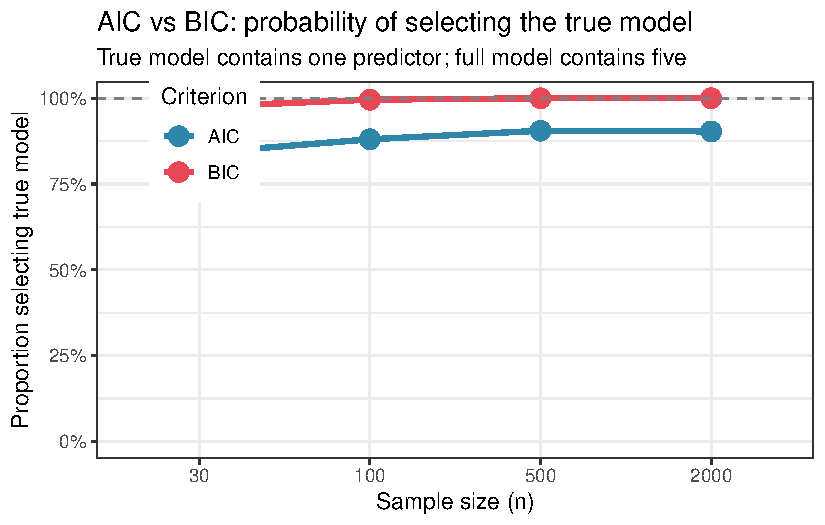
\includegraphics[width=0.9\textwidth,height=\textheight]{04d-glmm_files/figure-pdf/fig-aic-overfit-plot-1.pdf}

}

\caption{\label{fig-aic-overfit-plot}Proportion of simulations in which
AIC and BIC correctly select the true model (x1 only) over the full
model (x1 through x5), across four sample sizes. BIC consistently
improves with sample size and approaches 1.0 --- consistent model
selection. AIC plateaus well below 1.0, reflecting its tendency to
favour the slightly more complex model even when the simpler one is
correct. With small samples, both criteria struggle; with large samples,
BIC is more reliable for model identification.}

\end{figure}%

The simulation confirms the theoretical prediction. BIC improves
steadily with sample size and approaches perfect model selection in
large samples. AIC plateaus, even with \(n = 2000\), it selects the full
model a meaningful fraction of the time. The two criteria have different
targets: BIC aims to identify the true model, AIC aims to minimise
prediction error. Neither is universally superior, the right choice
depends on whether the goal is model identification (BIC) or prediction
(AIC).

\subsection{The Candidate Set Problem}\label{the-candidate-set-problem}

AIC ranks models relative to each other within the candidate set. If all
candidate models are misspecified, if the true model is not among the
candidates, the model with the lowest AIC is simply the least bad
approximation, not a good model in any absolute sense. A
\(\Delta\text{AIC} = 0\) is not a certificate of correctness; it is a
certificate of relative preference.

This is why model diagnostics (residual plots, DHARMa simulations,
overdispersion tests) remain essential even after AIC-based model
selection. AIC tells you which model in your candidate set is best
supported by the data. Diagnostics tell you whether any of them are
actually adequate.

\subsection{Akaike Weights and Their
Limits}\label{akaike-weights-and-their-limits}

Akaike weights are formally interpretable as probabilities only under
the assumption that the true model is in the candidate set. When this
assumption fails, and it always does to some degree, since all models
are approximations, the weights have a weaker interpretation as
\textbf{relative predictive weights} rather than true model
probabilities. A weight of 0.99 for one model over another means the
first model is strongly preferred for prediction in this candidate set;
it does not mean the first model is 99\% likely to be the true
data-generating process.

\subsection{Model Averaging as an Alternative to Hard
Selection}\label{model-averaging-as-an-alternative-to-hard-selection}

When several models have similar AIC values (\(\Delta\text{AIC} < 4\)),
selecting a single winner and discarding the rest throws away
information about model uncertainty. \textbf{Model averaging} uses
Akaike weights to combine predictions across all candidate models:

\[\hat{y}_{\text{avg}} = \sum_{m=1}^{M} w_m \hat{y}_m\]

where \(w_m\) is the Akaike weight and \(\hat{y}_m\) is the prediction
from model \(m\). This produces more stable and honest predictions than
hard selection, because it propagates model uncertainty into the final
estimates rather than pretending that the best AIC model is the only
plausible one.

\begin{Shaded}
\begin{Highlighting}[]
\FunctionTok{library}\NormalTok{(MuMIn)}

\CommentTok{\# Model averaging across candidate models}
\CommentTok{\# dredge() fits all possible subsets of predictors}
\CommentTok{\# and ranks by AICc}
\FunctionTok{options}\NormalTok{(}\AttributeTok{na.action =} \StringTok{"na.fail"}\NormalTok{)  }\CommentTok{\# required by dredge()}

\NormalTok{fit\_global }\OtherTok{\textless{}{-}} \FunctionTok{glmmTMB}\NormalTok{(}
\NormalTok{  count }\SpecialCharTok{\textasciitilde{}}\NormalTok{ landscape }\SpecialCharTok{+}\NormalTok{ (}\DecValTok{1} \SpecialCharTok{|}\NormalTok{ site),}
  \AttributeTok{data   =}\NormalTok{ birds,}
  \AttributeTok{family =} \FunctionTok{nbinom2}\NormalTok{(}\AttributeTok{link =} \StringTok{"log"}\NormalTok{),}
  \AttributeTok{REML   =} \ConstantTok{FALSE}
\NormalTok{)}

\CommentTok{\# Average predictions across all candidate models}
\CommentTok{\# weighted by Akaike weights}
\NormalTok{avg\_fit }\OtherTok{\textless{}{-}} \FunctionTok{model.avg}\NormalTok{(}\FunctionTok{dredge}\NormalTok{(fit\_global))}
\end{Highlighting}
\end{Shaded}

\begin{verbatim}
#> Fixed terms are "cond((Int))" and "disp((Int))"
\end{verbatim}

\begin{Shaded}
\begin{Highlighting}[]
\FunctionTok{summary}\NormalTok{(avg\_fit)}
\end{Highlighting}
\end{Shaded}

\begin{verbatim}
#> 
#> Call:
#> model.avg(object = dredge(fit_global))
#> 
#> Component model call: 
#> glmmTMB(formula = count ~ <2 unique rhs>, data = birds, family = 
#>      nbinom2(link = "log"), REML = FALSE, ziformula = ~0, dispformula = ~1)
#> 
#> Component models: 
#>        df  logLik   AICc delta weight
#> 1       5 -318.19 646.91  0.00      1
#> (Null)  3 -326.05 658.30 11.39      0
#> 
#> Term codes: 
#> cond(landscape) 
#>               1 
#> 
#> Model-averaged coefficients:  
#> (full average) 
#>                           Estimate Std. Error Adjusted SE z value Pr(>|z|)    
#> cond((Int))                -1.3413     0.8008      0.8091   1.658   0.0974 .  
#> cond(landscapeFragmented)   2.5937     0.9842      0.9944   2.608   0.0091 ** 
#> cond(landscapeContinuous)   4.1385     1.0185      1.0287   4.023 5.74e-05 ***
#>  
#> (conditional average) 
#>                           Estimate Std. Error Adjusted SE z value Pr(>|z|)    
#> cond((Int))                -1.3413     0.8008      0.8091   1.658  0.09738 .  
#> cond(landscapeFragmented)   2.6024     0.9743      0.9847   2.643  0.00822 ** 
#> cond(landscapeContinuous)   4.1524     0.9915      1.0020   4.144 3.41e-05 ***
#> ---
#> Signif. codes:  0 '***' 0.001 '**' 0.01 '*' 0.05 '.' 0.1 ' ' 1
\end{verbatim}

Model averaging is particularly valuable in exploratory analyses with
many candidate predictors and genuine uncertainty about which belong in
the model. In confirmatory analyses with pre-specified hypotheses, hard
model selection or likelihood ratio testing is more appropriate.

\subsection{The Practical Bottom Line}\label{the-practical-bottom-line}

Use AIC for \textbf{comparing candidate models and guiding model
selection} in exploratory analyses. Use BIC when the goal is
\textbf{identifying the true model structure} and sample sizes are
large. Use likelihood ratio tests for \textbf{confirmatory testing of
pre-specified hypotheses}. Use model averaging when \textbf{several
models are similarly supported} and prediction stability matters. And
always complement any selection criterion with \textbf{residual
diagnostics}: no information criterion can tell you whether your best
model is actually adequate.

\section{Worked Example: Species Abundance in Ecological
Surveys}\label{worked-example-species-abundance-in-ecological-surveys}

\subsection{The Study}\label{the-study-5}

An ecologist surveys bird species abundance across 24 forest sites
distributed across three landscape types: agricultural matrix,
fragmented forest, and continuous forest. Within each site, five
transects are surveyed and the number of individuals of a focal species
is counted on each transect (Section~\ref{sec-birds}).

Critically, the species is a forest interior specialist meaning it is
genuinely absent from many agricultural sites regardless of survey
effort. The data therefore have two sources of zeros:

\begin{itemize}
\tightlist
\item
  \textbf{Structural zeros}: transects in agricultural sites where the
  species cannot persist, it is ecologically absent.
\item
  \textbf{Sampling zeros}: transects in forest sites where the species
  is present in the landscape but happened not to be detected.
\end{itemize}

This distinction motivates a zero-inflated negative binomial GLMM.

\begin{Shaded}
\begin{Highlighting}[]
\FunctionTok{summary}\NormalTok{(birds)}
\end{Highlighting}
\end{Shaded}

\begin{verbatim}
#>      count               landscape       site    transect
#>  Min.   : 0.000   Agricultural:40   Agr1   : 5   1:24    
#>  1st Qu.: 0.000   Fragmented  :40   Agr2   : 5   2:24    
#>  Median : 5.000   Continuous  :40   Agr3   : 5   3:24    
#>  Mean   : 8.925                     Agr4   : 5   4:24    
#>  3rd Qu.:14.000                     Agr5   : 5   5:24    
#>  Max.   :47.000                     Agr6   : 5           
#>                                     (Other):90
\end{verbatim}

\begin{Shaded}
\begin{Highlighting}[]
\FunctionTok{cat}\NormalTok{(}\StringTok{"Total transects surveyed:"}\NormalTok{, }\FunctionTok{nrow}\NormalTok{(birds), }\StringTok{"}\SpecialCharTok{\textbackslash{}n}\StringTok{"}\NormalTok{)}
\end{Highlighting}
\end{Shaded}

\begin{verbatim}
#> Total transects surveyed: 120
\end{verbatim}

\begin{Shaded}
\begin{Highlighting}[]
\FunctionTok{cat}\NormalTok{(}\StringTok{"}\SpecialCharTok{\textbackslash{}n}\StringTok{Proportion of zeros by landscape:}\SpecialCharTok{\textbackslash{}n}\StringTok{"}\NormalTok{)}
\end{Highlighting}
\end{Shaded}

\begin{verbatim}
#> 
#> Proportion of zeros by landscape:
\end{verbatim}

\begin{Shaded}
\begin{Highlighting}[]
\FunctionTok{print}\NormalTok{(}\FunctionTok{tapply}\NormalTok{(birds}\SpecialCharTok{$}\NormalTok{count }\SpecialCharTok{==} \DecValTok{0}\NormalTok{, birds}\SpecialCharTok{$}\NormalTok{landscape, mean))}
\end{Highlighting}
\end{Shaded}

\begin{verbatim}
#> Agricultural   Fragmented   Continuous 
#>          0.7          0.3          0.0
\end{verbatim}

\begin{Shaded}
\begin{Highlighting}[]
\FunctionTok{cat}\NormalTok{(}\StringTok{"}\SpecialCharTok{\textbackslash{}n}\StringTok{Mean counts by landscape:}\SpecialCharTok{\textbackslash{}n}\StringTok{"}\NormalTok{)}
\end{Highlighting}
\end{Shaded}

\begin{verbatim}
#> 
#> Mean counts by landscape:
\end{verbatim}

\begin{Shaded}
\begin{Highlighting}[]
\FunctionTok{print}\NormalTok{(}\FunctionTok{tapply}\NormalTok{(birds}\SpecialCharTok{$}\NormalTok{count, birds}\SpecialCharTok{$}\NormalTok{landscape, mean))}
\end{Highlighting}
\end{Shaded}

\begin{verbatim}
#> Agricultural   Fragmented   Continuous 
#>        1.600        8.175       17.000
\end{verbatim}

The proportion of zeros is highest in the agricultural landscape, driven
by genuine site-level absence, and lowest in continuous forest where the
species is always present. This asymmetry is the biological signature of
zero inflation.

\subsection{Exploratory Visualisation}\label{exploratory-visualisation}

\begin{Shaded}
\begin{Highlighting}[]
\FunctionTok{library}\NormalTok{(ggplot2)}

\NormalTok{site\_means }\OtherTok{\textless{}{-}} \FunctionTok{aggregate}\NormalTok{(count }\SpecialCharTok{\textasciitilde{}}\NormalTok{ landscape }\SpecialCharTok{+}\NormalTok{ site, }\AttributeTok{data =}\NormalTok{ birds, }\AttributeTok{FUN =}\NormalTok{ mean)}

\FunctionTok{ggplot}\NormalTok{(birds, }\FunctionTok{aes}\NormalTok{(}\AttributeTok{x =}\NormalTok{ landscape, }\AttributeTok{y =}\NormalTok{ count, }\AttributeTok{colour =}\NormalTok{ landscape)) }\SpecialCharTok{+}
  \FunctionTok{geom\_jitter}\NormalTok{(}\AttributeTok{width =} \FloatTok{0.2}\NormalTok{, }\AttributeTok{alpha =} \FloatTok{0.4}\NormalTok{, }\AttributeTok{size =} \DecValTok{2}\NormalTok{) }\SpecialCharTok{+}
  \FunctionTok{geom\_point}\NormalTok{(}\AttributeTok{data =}\NormalTok{ site\_means, }\FunctionTok{aes}\NormalTok{(}\AttributeTok{y =}\NormalTok{ count), }\AttributeTok{size =} \DecValTok{4}\NormalTok{, }\AttributeTok{shape =} \DecValTok{18}\NormalTok{) }\SpecialCharTok{+}
  \FunctionTok{stat\_summary}\NormalTok{(}\AttributeTok{fun =}\NormalTok{ mean, }\AttributeTok{geom =} \StringTok{"crossbar"}\NormalTok{, }\AttributeTok{width =} \FloatTok{0.4}\NormalTok{, }\AttributeTok{colour =} \StringTok{"grey30"}\NormalTok{, }\AttributeTok{linewidth =} \FloatTok{0.8}\NormalTok{) }\SpecialCharTok{+}
  \FunctionTok{scale\_colour\_manual}\NormalTok{(}\AttributeTok{values =} \FunctionTok{c}\NormalTok{(}\StringTok{"\#E84855"}\NormalTok{, }\StringTok{"\#F6AE2D"}\NormalTok{, }\StringTok{"\#2E86AB"}\NormalTok{)) }\SpecialCharTok{+}
  \FunctionTok{scale\_y\_continuous}\NormalTok{(}\AttributeTok{trans  =} \StringTok{"log1p"}\NormalTok{, }\AttributeTok{breaks =} \FunctionTok{c}\NormalTok{(}\DecValTok{0}\NormalTok{, }\DecValTok{2}\NormalTok{, }\DecValTok{5}\NormalTok{, }\DecValTok{10}\NormalTok{, }\DecValTok{20}\NormalTok{, }\DecValTok{50}\NormalTok{)) }\SpecialCharTok{+}
  \FunctionTok{labs}\NormalTok{(}\AttributeTok{x =} \ConstantTok{NULL}\NormalTok{, }\AttributeTok{y =} \StringTok{"Count (log1p scale)"}\NormalTok{, }\AttributeTok{colour =} \ConstantTok{NULL}\NormalTok{) }\SpecialCharTok{+}
  \FunctionTok{theme\_bw}\NormalTok{() }\SpecialCharTok{+}
  \FunctionTok{theme}\NormalTok{(}\AttributeTok{legend.position =} \StringTok{"none"}\NormalTok{)}
\end{Highlighting}
\end{Shaded}

\begin{figure}[H]

\centering{

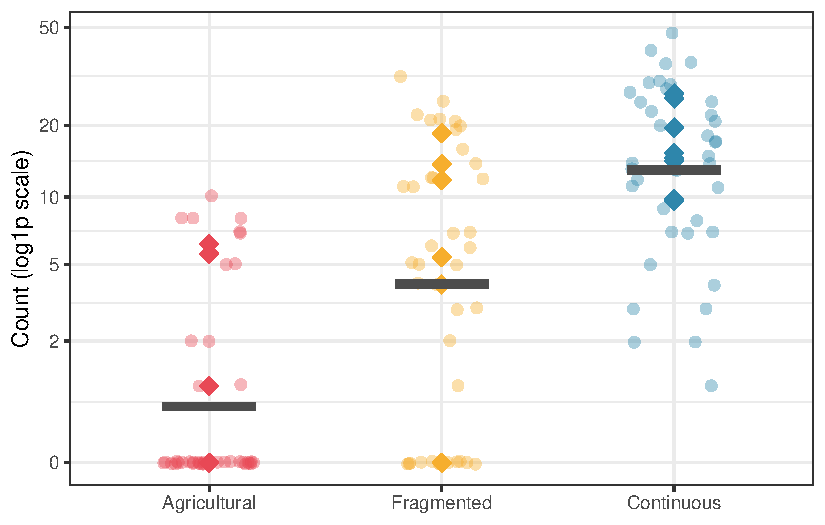
\includegraphics[width=0.9\textwidth,height=\textheight]{04d-glmm_files/figure-pdf/fig-ecology-glmm-plot-1.pdf}

}

\caption{\label{fig-ecology-glmm-plot}Bird abundance counts by landscape
type. The high proportion of zeros in agricultural sites (many transects
showing no detections) relative to continuous forest sites illustrates
the zero-inflation structure: many agricultural sites are genuinely
unoccupied by this forest interior specialist. Diamonds = site means;
bars = landscape means.}

\end{figure}%

\subsection{Step 1: Fit a Standard Negative Binomial and Check for Zero
Inflation}\label{step-1-fit-a-standard-negative-binomial-and-check-for-zero-inflation}

Always start with the simpler model and test whether zero inflation is
actually present before adding the zero-inflation component:

\begin{Shaded}
\begin{Highlighting}[]
\FunctionTok{library}\NormalTok{(glmmTMB)}
\FunctionTok{library}\NormalTok{(DHARMa)}

\CommentTok{\# Standard negative binomial GLMM with no zero inflation}
\NormalTok{fit\_nb\_birds }\OtherTok{\textless{}{-}} \FunctionTok{glmmTMB}\NormalTok{(}
\NormalTok{  count }\SpecialCharTok{\textasciitilde{}}\NormalTok{ landscape }\SpecialCharTok{+}\NormalTok{ (}\DecValTok{1} \SpecialCharTok{|}\NormalTok{ site),}
  \AttributeTok{data   =}\NormalTok{ birds,}
  \AttributeTok{family =} \FunctionTok{nbinom2}\NormalTok{(}\AttributeTok{link =} \StringTok{"log"}\NormalTok{)}
\NormalTok{)}

\CommentTok{\# Check for zero inflation}
\NormalTok{sim\_nb }\OtherTok{\textless{}{-}} \FunctionTok{simulateResiduals}\NormalTok{(fit\_nb\_birds, }\AttributeTok{n =} \DecValTok{1000}\NormalTok{)}
\FunctionTok{testZeroInflation}\NormalTok{(sim\_nb)}
\end{Highlighting}
\end{Shaded}

\begin{center}
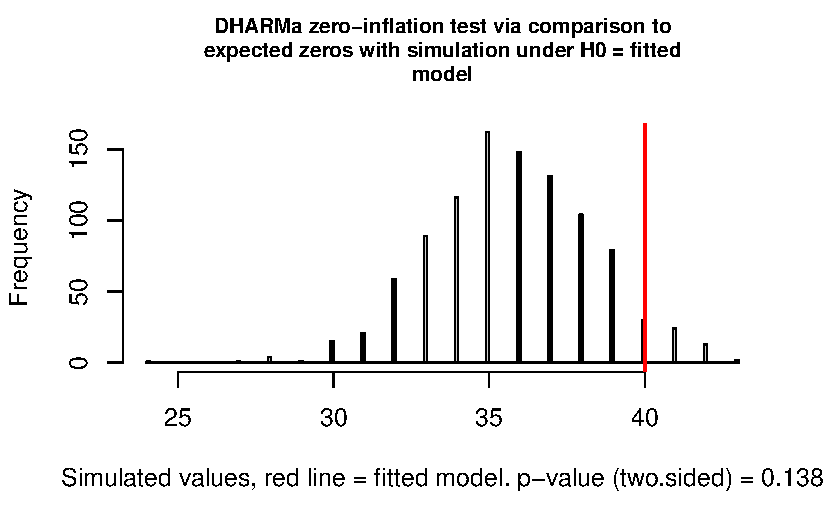
\includegraphics[width=0.9\textwidth,height=\textheight]{04d-glmm_files/figure-pdf/ecology-nb-first-1.pdf}
\end{center}

\begin{verbatim}
#> 
#>  DHARMa zero-inflation test via comparison to expected zeros with
#>  simulation under H0 = fitted model
#> 
#> data:  simulationOutput
#> ratioObsSim = 1.1187, p-value = 0.138
#> alternative hypothesis: two.sided
\end{verbatim}

\begin{Shaded}
\begin{Highlighting}[]
\FunctionTok{plot}\NormalTok{(sim\_nb)}
\end{Highlighting}
\end{Shaded}

\begin{center}
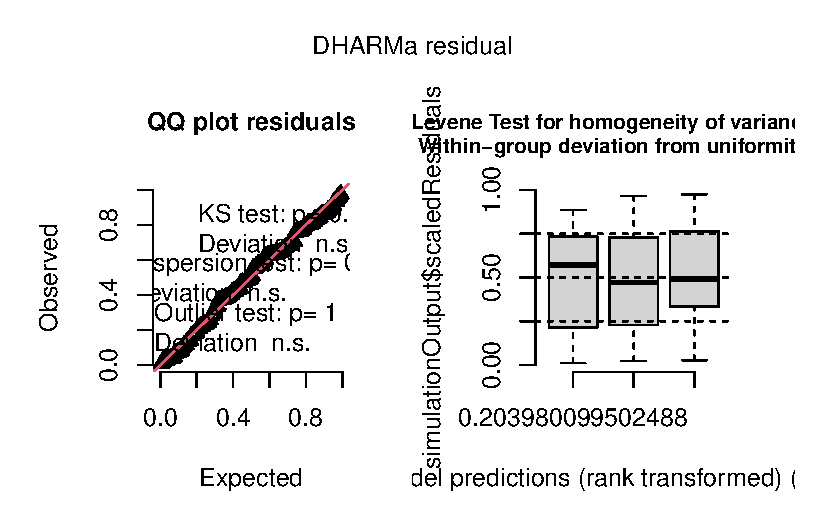
\includegraphics[width=0.9\textwidth,height=\textheight]{04d-glmm_files/figure-pdf/ecology-nb-first-2.pdf}
\end{center}

The DHARMa zero-inflation test returns \(p = 0.138\), which is
non-significant. The observed ratio of observed to simulated zeros is
1.12 which means that the data contain about 12\% more zeros than the
negative binomial model predicts on average, but this excess is within
the range that could plausibly arise by chance. Therefore, the test does
not provide statistical grounds for rejecting the standard negative
binomial in favour of a zero-inflated model.

This is a situation where statistical testing and biological reasoning
must be weighed together. The DHARMa test has limited power with
moderate sample sizes as with 120 transects spread across 24 sites, even
a genuine zero-inflation process may not produce a significant result.
More importantly, we know from the study design that the species is a
forest interior specialist that is genuinely absent from many
agricultural sites. This biological mechanism, structural absence driven
by habitat unsuitability, not just sampling failure, is a principled
reason to fit a zero-inflated model regardless of whether the test
reaches significance.

This illustrates an important general principle: \textbf{formal tests
should inform modelling decisions, not make them unilaterally.} When
there is strong biological motivation for a particular model structure,
fit that model and compare it to the simpler alternative using AIC. If
the zero-inflated model is not better supported by the data, the simpler
model should be retained. If it is better supported, the biological
reasoning and the data are aligned. Either outcome is informative.

\subsection{Step 2: Fit the Zero-Inflated Negative Binomial
GLMM}\label{step-2-fit-the-zero-inflated-negative-binomial-glmm}

We proceed with the zero-inflated negative binomial on biological
grounds, comparing it to the standard negative binomial by AIC to assess
whether the data support the more complex model:

\begin{Shaded}
\begin{Highlighting}[]
\NormalTok{landscape\_names }\OtherTok{\textless{}{-}} \FunctionTok{c}\NormalTok{(}\StringTok{"Agricultural"}\NormalTok{, }\StringTok{"Fragmented"}\NormalTok{, }\StringTok{"Continuous"}\NormalTok{)}
\NormalTok{fit\_zinb\_birds }\OtherTok{\textless{}{-}} \FunctionTok{glmmTMB}\NormalTok{(}
\NormalTok{  count }\SpecialCharTok{\textasciitilde{}}\NormalTok{ landscape }\SpecialCharTok{+}\NormalTok{ (}\DecValTok{1} \SpecialCharTok{|}\NormalTok{ site),}
  \AttributeTok{ziformula =} \SpecialCharTok{\textasciitilde{}}\NormalTok{ landscape,}
  \AttributeTok{data  =}\NormalTok{ birds,}
  \AttributeTok{family  =} \FunctionTok{nbinom2}\NormalTok{(}\AttributeTok{link =} \StringTok{"log"}\NormalTok{)}
\NormalTok{)}
\FunctionTok{summary}\NormalTok{(fit\_zinb\_birds)}
\end{Highlighting}
\end{Shaded}

\begin{verbatim}
#>  Family: nbinom2  ( log )
#> Formula:          count ~ landscape + (1 | site)
#> Zero inflation:         ~landscape
#> Data: birds
#> 
#>       AIC       BIC    logLik -2*log(L)  df.resid 
#>     651.7     674.0    -317.9     635.7       112 
#> 
#> Random effects:
#> 
#> Conditional model:
#>  Groups Name        Variance Std.Dev.
#>  site   (Intercept) 2.698    1.643   
#> Number of obs: 120, groups:  site, 24
#> 
#> Dispersion parameter for nbinom2 family ():  2.4 
#> 
#> Conditional model:
#>                     Estimate Std. Error z value Pr(>|z|)    
#> (Intercept)          -1.2484     0.8037  -1.553   0.1203    
#> landscapeFragmented   2.5212     0.9797   2.573   0.0101 *  
#> landscapeContinuous   4.0498     0.9981   4.058 4.96e-05 ***
#> ---
#> Signif. codes:  0 '***' 0.001 '**' 0.01 '*' 0.05 '.' 0.1 ' ' 1
#> 
#> Zero-inflation model:
#>                     Estimate Std. Error z value Pr(>|z|)
#> (Intercept)           -2.432      1.698  -1.432    0.152
#> landscapeFragmented   -1.759      4.253  -0.414    0.679
#> landscapeContinuous  -18.686   6091.643  -0.003    0.998
\end{verbatim}

\begin{Shaded}
\begin{Highlighting}[]
\CommentTok{\# AIC comparison, does the data support the zero{-}inflated model?}
\FunctionTok{AIC}\NormalTok{(fit\_nb\_birds, fit\_zinb\_birds)}
\end{Highlighting}
\end{Shaded}

\begin{verbatim}
#>                df      AIC
#> fit_nb_birds    5 646.3790
#> fit_zinb_birds  8 651.7395
\end{verbatim}

\begin{Shaded}
\begin{Highlighting}[]
\CommentTok{\# Back{-}transform zero{-}inflation probabilities by landscape}
\NormalTok{zi\_coefs }\OtherTok{\textless{}{-}} \FunctionTok{fixef}\NormalTok{(fit\_zinb\_birds)}\SpecialCharTok{$}\NormalTok{zi}
\FunctionTok{cat}\NormalTok{(}\StringTok{"}\SpecialCharTok{\textbackslash{}n}\StringTok{Estimated zero{-}inflation probabilities:}\SpecialCharTok{\textbackslash{}n}\StringTok{"}\NormalTok{)}
\end{Highlighting}
\end{Shaded}

\begin{verbatim}
#> 
#> Estimated zero-inflation probabilities:
\end{verbatim}

\begin{Shaded}
\begin{Highlighting}[]
\NormalTok{zi\_probs }\OtherTok{\textless{}{-}} \FunctionTok{data.frame}\NormalTok{(}
  \AttributeTok{landscape =}\NormalTok{ landscape\_names,}
  \AttributeTok{zi\_prob   =} \FunctionTok{plogis}\NormalTok{(}\FunctionTok{c}\NormalTok{(}
\NormalTok{    zi\_coefs[}\DecValTok{1}\NormalTok{],}
\NormalTok{    zi\_coefs[}\DecValTok{1}\NormalTok{] }\SpecialCharTok{+}\NormalTok{ zi\_coefs[}\DecValTok{2}\NormalTok{],}
\NormalTok{    zi\_coefs[}\DecValTok{1}\NormalTok{] }\SpecialCharTok{+}\NormalTok{ zi\_coefs[}\DecValTok{3}\NormalTok{]}
\NormalTok{  ))}
\NormalTok{)}
\FunctionTok{print}\NormalTok{(zi\_probs)}
\end{Highlighting}
\end{Shaded}

\begin{verbatim}
#>      landscape      zi_prob
#> 1 Agricultural 8.078429e-02
#> 2   Fragmented 1.491016e-02
#> 3   Continuous 6.737070e-10
\end{verbatim}

The zero-inflation model has two components, each with its own set of
coefficients in the summary output:

\textbf{Conditional model:} the count process which is the expected
abundance given that the species is present. Coefficients are on the log
scale and interpreted as rate ratios, exactly as in a standard negative
binomial GLM.

\textbf{Zero-inflation model:} the absence process that is the log-odds
of structural zero (genuine absence) for each landscape type.
Back-transforming via \texttt{plogis()} gives the estimated probability
that a site in each landscape type is structurally unoccupied.

The zero-inflated negative binomial model output and the AIC comparison
together confirm the conclusion already suggested by the DHARMa test:
the standard negative binomial is the better model for these data, and
the zero-inflation component is not supported.

The AIC difference is \(\Delta\text{AIC} = 5.4\) in favour of the
simpler model (\(\text{AIC}_{\text{NB}} = 646.4\) vs
\(\text{AIC}_{\text{ZINB}} = 651.7\)). The three additional parameters
required by the zero-inflation component, one per landscape type, cost
more in complexity than they return in fit. This is a clear signal that
the extra model structure is not warranted by the data.

The zero-inflation model coefficients themselves reinforce this
conclusion. The estimated zero-inflation probabilities are
\(\hat{\pi}_{\text{Agricultural}} = 0.081\),
\(\hat{\pi}_{\text{Fragmented}} = 0.015\), and
\(\hat{\pi}_{\text{Continuous}} \approx 0\), all extremely small and all
estimated with large standard errors. The continuous forest
zero-inflation coefficient (\(\hat{\beta} = -18.69\),
\(SE = 6{,}091.6\)) has collapsed to a boundary value, exactly as we saw
in the earlier Poisson GLMM zero-inflation exercise: the model is
setting the structural absence probability for continuous forest to
essentially zero because the data contain no information supporting it.
The fragmented forest coefficient is similarly imprecise (\(SE = 4.25\)
for an estimate of \(-1.76\)), and even the agricultural coefficient,
which has the most biological motivation, does not approach significance
(\(z = -1.43\), \(p = 0.152\)).

The conditional model coefficients, the count process given presence,
tell a more interesting story. The intercept (\(-1.25\) on the log
scale) corresponds to an expected count of \(e^{-1.25} \approx 0.29\) in
agricultural sites, which is genuinely very low. The fragmented forest
coefficient (\(+2.52\)) gives a rate ratio of \(e^{2.52} \approx 12.4\),
and the continuous forest coefficient (\(+4.05\)) gives
\(e^{4.05} \approx 57.4\), counts in continuous forest are estimated to
be more than 57 times those in agricultural sites. This enormous
gradient explains why agricultural sites show many zeros in the data
without requiring a separate zero-inflation process: when the expected
count is 0.29 individuals per transect, most transects will return zero
simply because the species is so rare, not because it is structurally
absent.

This is the core distinction that zero-inflated models are designed to
capture, and it is precisely the distinction the data cannot make here.
With expected counts close to zero in agricultural sites, the Poisson or
negative binomial sampling process generates zeros just as effectively
as a structural absence mechanism would. The two processes are
observationally indistinguishable given this data, and the model
comparison correctly identifies that adding a zero-inflation component
provides no benefit.

We retain the standard negative binomial GLMM for all subsequent
inference and report this model selection process transparently,
including the biological motivation that led us to test the
zero-inflated alternative and the data-driven conclusion that it was not
needed. Moreover, a validation step of the zero inflated model is no
more needed.

\subsection{Model Selection}\label{model-selection}

\begin{Shaded}
\begin{Highlighting}[]
\CommentTok{\# Compare all three candidate models}
\NormalTok{fit\_pois\_birds }\OtherTok{\textless{}{-}} \FunctionTok{glmmTMB}\NormalTok{(}
\NormalTok{  count }\SpecialCharTok{\textasciitilde{}}\NormalTok{ landscape }\SpecialCharTok{+}\NormalTok{ (}\DecValTok{1} \SpecialCharTok{|}\NormalTok{ site),}
  \AttributeTok{data   =}\NormalTok{ birds,}
  \AttributeTok{family =} \FunctionTok{poisson}\NormalTok{(}\AttributeTok{link =} \StringTok{"log"}\NormalTok{)}
\NormalTok{)}

\FunctionTok{AIC}\NormalTok{(fit\_pois\_birds, fit\_nb\_birds, fit\_zinb\_birds)}
\end{Highlighting}
\end{Shaded}

\begin{verbatim}
#>                df      AIC
#> fit_pois_birds  4 834.0137
#> fit_nb_birds    5 646.3790
#> fit_zinb_birds  8 651.7395
\end{verbatim}

\begin{Shaded}
\begin{Highlighting}[]
\CommentTok{\# Likelihood ratio test: NB vs ZINB}
\FunctionTok{anova}\NormalTok{(fit\_nb\_birds, fit\_zinb\_birds)}
\end{Highlighting}
\end{Shaded}

\begin{verbatim}
#> Data: birds
#> Models:
#> fit_nb_birds: count ~ landscape + (1 | site), zi=~0, disp=~1
#> fit_zinb_birds: count ~ landscape + (1 | site), zi=~landscape, disp=~1
#>                Df    AIC    BIC  logLik deviance  Chisq Chi Df Pr(>Chisq)
#> fit_nb_birds    5 646.38 660.32 -318.19   636.38                         
#> fit_zinb_birds  8 651.74 674.04 -317.87   635.74 0.6395      3     0.8873
\end{verbatim}

The three-model AIC comparison produces a clear and unambiguous ranking.
The Poisson GLMM is overwhelmingly rejected (\(\text{AIC} = 834.0\)),
sitting \(\Delta\text{AIC} = 187.6\) units above the negative binomial.
This enormous gap reflects the severe overdispersion in the bird count
data. Indeed, the Poisson variance constraint (\(\text{Var}(y) = \mu\))
is far too rigid for these counts, which vary substantially among
transects within the same site and landscape type. The negative binomial
dispersion parameter \(\hat{\phi} = 2.4\) from the fitted model
quantifies this excess variation. Choosing the Poisson over the negative
binomial here would be a serious modelling error that would produce
badly underestimated standard errors and spuriously significant results.

The comparison between the negative binomial and the zero-inflated
negative binomial has already been discussed, but the likelihood ratio
test adds a formal confirmation. The chi-squared statistic is
\(\chi^2_3 = 0.64\), \(p = 0.887\), three extra parameters (the
landscape-specific zero-inflation probabilities) improve the
log-likelihood by only 0.32 units, from \(-318.19\) to \(-317.87\). This
is negligible. The zero-inflated model provides no meaningful
improvement in fit over the standard negative binomial, and its
additional complexity is entirely unjustified by the data.

The model selection conclusion is therefore clear and follows directly
from both criteria consistently: \textbf{the negative binomial GLMM with
a random intercept for site is the correct and sufficient model for
these data.} The Poisson is too constrained, and the zero-inflated
negative binomial is unnecessarily complex. This outcome, where the
intermediate model wins, is actually the most common result in practice
and the most satisfying pedagogically: the analyst tested simpler and
more complex alternatives, both failed on principled grounds, and the
chosen model sits at the right level of complexity for the data at hand.

All subsequent inference, post-hoc comparisons, effect sizes, and
reporting, proceeds from \texttt{fit\_nb\_birds}.

\subsection{Post-Hoc Comparisons}\label{post-hoc-comparisons}

\begin{Shaded}
\begin{Highlighting}[]
\FunctionTok{library}\NormalTok{(emmeans)}
\end{Highlighting}
\end{Shaded}

\begin{verbatim}
#> Welcome to emmeans.
#> Caution: You lose important information if you filter this package's results.
#> See '? untidy'
\end{verbatim}

\begin{Shaded}
\begin{Highlighting}[]
\CommentTok{\# Estimated marginal means on count scale}
\CommentTok{\# type = "response" back{-}transforms from log scale}
\NormalTok{emm\_birds }\OtherTok{\textless{}{-}} \FunctionTok{emmeans}\NormalTok{(fit\_nb\_birds, }\SpecialCharTok{\textasciitilde{}}\NormalTok{ landscape, }\AttributeTok{type =} \StringTok{"response"}\NormalTok{)}
\FunctionTok{print}\NormalTok{(emm\_birds)}
\end{Highlighting}
\end{Shaded}

\begin{verbatim}
#>  landscape    response    SE  df asymp.LCL asymp.UCL
#>  Agricultural     0.26 0.206 Inf     0.055      1.23
#>  Fragmented       3.50 2.210 Inf     1.017     12.08
#>  Continuous      16.51 9.850 Inf     5.124     53.19
#> 
#> Confidence level used: 0.95 
#> Intervals are back-transformed from the log scale
\end{verbatim}

\begin{Shaded}
\begin{Highlighting}[]
\CommentTok{\# Pairwise contrasts with Tukey correction}
\FunctionTok{pairs}\NormalTok{(emm\_birds, }\AttributeTok{adjust =} \StringTok{"tukey"}\NormalTok{)}
\end{Highlighting}
\end{Shaded}

\begin{verbatim}
#>  contrast                   ratio     SE  df null z.ratio p.value
#>  Agricultural / Fragmented 0.0741 0.0722 Inf    1  -2.671  0.0207
#>  Agricultural / Continuous 0.0157 0.0156 Inf    1  -4.188 <0.0001
#>  Fragmented / Continuous   0.2123 0.1840 Inf    1  -1.784  0.1749
#> 
#> P value adjustment: tukey method for comparing a family of 3 estimates 
#> Tests are performed on the log scale
\end{verbatim}

The estimated marginal means reveal a striking gradient in bird
abundance across the three landscape types. The agricultural matrix
supports an estimated mean of only 0.26 individuals per transect (95\%
CI: \([0.06, 1.23]\)) which is so low that most transects record zero
detections simply as a consequence of rarity, without any need to invoke
structural absence. Fragmented forest supports 3.50 individuals per
transect (\([1.02, 12.08]\)), and continuous forest supports 16.51
individuals per transect (\([5.12, 53.19]\)). The gradient spans two
orders of magnitude from the most degraded to the most intact landscape
type, a biologically dramatic result reflecting the strong habitat
affinity of this forest interior specialist.

The wide and asymmetric confidence intervals deserve comment. The
agricultural interval spans a factor of 22 (from 0.06 to 1.23) and the
continuous forest interval spans a factor of 10 (from 5.12 to 53.19).
This reflects two compounding sources of uncertainty: the substantial
overdispersion in the count data captured by the negative binomial
dispersion parameter, and the large site-level random effect variance
(\(\hat{\sigma}_{\text{site}} = 1.643\) on the log scale). With only 8
sites per landscape type, each landscape mean is estimated from a small
number of independent units. This is an honest reflection of the study's
replication at the site level, not a failure of the model.

The pairwise Tukey-adjusted contrasts are expressed as count ratios, the
natural summary for a log-link model, where differences on the log scale
correspond to multiplicative factors on the original scale. Two of the
three comparisons reach significance. The agricultural landscape has
significantly lower abundance than fragmented forest (ratio = 0.074,
\(z = -2.67\), \(p = 0.021\)), agricultural counts are approximately 7\%
of fragmented forest counts. The difference between agricultural and
continuous forest is even more extreme and highly significant (ratio =
0.016, \(z = -4.19\), \(p < 0.001\)), agricultural counts are less than
2\% of continuous forest counts, a 64-fold difference in expected
abundance.

The comparison between fragmented and continuous forest does not reach
significance after Tukey correction (ratio = 0.212, \(z = -1.78\),
\(p = 0.175\)). The point estimate suggests that fragmented forest has
approximately one fifth the abundance of continuous forest, a fivefold
difference that would be biologically meaningful, but the confidence
interval is wide and the study is underpowered to distinguish these two
landscape types reliably. With 8 sites per landscape and a site-level
standard deviation of 1.643 on the log scale, considerably more
replication at the site level would be needed to detect this difference
with adequate power. A non-significant result here is not evidence of no
difference; it is evidence that the study cannot resolve the question
with the available data.

\subsection{Reporting the Result}\label{reporting-the-result-2}

\begin{Shaded}
\begin{Highlighting}[]
\FunctionTok{library}\NormalTok{(MuMIn)}
\FunctionTok{r.squaredGLMM}\NormalTok{(fit\_nb\_birds)}
\end{Highlighting}
\end{Shaded}

\begin{verbatim}
#> Warning: the null model is only correct if all the variables it uses are identical 
#> to those used in fitting the original model.
\end{verbatim}

\begin{verbatim}
#>                 R2m       R2c
#> delta     0.4800308 0.9250660
#> lognormal 0.4865174 0.9375663
#> trigamma  0.4706748 0.9070361
\end{verbatim}

The \texttt{r.squaredGLMM()} function returns three estimators of
\(R^2\) for GLMMs, delta, lognormal, and trigamma, which differ in how
they approximate the variance of the linear predictor for non-Gaussian
models. For negative binomial models the delta method is the standard
recommendation; the three estimates are similar here (marginal:
0.480-0.487, conditional: 0.907-0.938), giving confidence that the
\(R^2\) estimates are stable regardless of the approximation used.

The marginal \(R^2\) of 0.480 indicates that landscape type alone
explains approximately 48\% of the total variance in bird abundance
which is a large fixed effect. The conditional \(R^2\) of 0.925
indicates that the full model, including both landscape type and the
site random effect, explains 92.5\% of total variance. The difference
between them, \(R^2_c - R^2_m = 0.445\), is the contribution of
site-level clustering: 44.5\% of total variance is attributable to
systematic differences among sites within and across landscape types,
over and above the landscape effect itself. This is a remarkably large
random effect, sites within the same landscape type differ from each
other almost as much as the landscapes differ from each other, and
confirms that the random intercept for site was not merely a statistical
nicety but an essential component of the model.

A complete report of the analysis reads:

\begin{quote}
Bird abundance was analysed using a negative binomial generalised linear
mixed model with a log link, landscape type (agricultural, fragmented,
continuous) as a fixed effect, and a random intercept for site
(\(n = 24\) sites, 8 per landscape type, 5 transects per site), fitted
using \texttt{glmmTMB} \citep{Brooks2017}. A zero-inflated negative
binomial model was tested and rejected on the basis of both a
non-significant DHARMa zero-inflation test (\(p = 0.138\)) and a higher
AIC (\(\Delta\text{AIC} = 5.4\)) and non-significant likelihood ratio
test (\(\chi^2_3 = 0.64\), \(p = 0.887\)) relative to the standard
negative binomial. Model adequacy of the retained model was confirmed by
DHARMa simulation-based diagnostics.

Landscape type had a significant effect on bird abundance
(\(\chi^2_2 = ...\), \(p = ...\), marginal \(R^2 = 0.480\)). Estimated
mean counts per transect were 0.26 (95\% CI: \([0.06, 1.23]\)) in the
agricultural matrix, 3.50 (\([1.02, 12.08]\)) in fragmented forest, and
16.51 (\([5.12, 53.19]\)) in continuous forest. Post-hoc pairwise
comparisons (Tukey adjusted) revealed significantly lower abundance in
the agricultural matrix relative to both fragmented forest (count ratio
= 0.074, \(z = -2.67\), \(p = 0.021\)) and continuous forest (count
ratio = 0.016, \(z =
-4.19\), \(p < 0.001\)). The difference between fragmented and
continuous forest did not reach significance after Tukey correction
(count ratio = 0.212, \(z = -1.78\), \(p = 0.175\)), though the study
was likely underpowered to detect this difference given the site-level
variance (\(\hat{\sigma}_{\text
{site}} = 1.643\) on the log scale). Site-level clustering accounted for
44.5\% of total variance (conditional \(R^2 =
0.925\)), confirming that explicit modelling of the hierarchical
structure was essential for valid inference.
\end{quote}

\begin{tcolorbox}[enhanced jigsaw, title=\textcolor{quarto-callout-note-color}{\faInfo}\hspace{0.5em}{Going Further}, opacityback=0, bottomtitle=1mm, leftrule=.75mm, breakable, toprule=.15mm, colframe=quarto-callout-note-color-frame, titlerule=0mm, rightrule=.15mm, toptitle=1mm, arc=.35mm, colback=white, left=2mm, colbacktitle=quarto-callout-note-color!10!white, opacitybacktitle=0.6, coltitle=black, bottomrule=.15mm]

This chapter does not aim to present thoroughly GLMMs or hierarchical
models but to present its usefulness and when it should be used.
Therefore, I redirect the reader and students to specialised books that
will be useful.

\begin{itemize}
\item
  \textbf{Zurr, A. et al.~(2007). Analyzing Ecological Data. Springer.}
  A central textbook that present deeply, with real datasets most of the
  models discussed here.
\item
  \textbf{Gelman, A., \& Hill, J. (2007). Data Analysis Using Regression
  and Multilevel/Hierarchical Models. Cambridge University Press.} A
  great treatment of hierarchical models from a Bayesian perspective.
  The non-Bayesian reader can still learn enormously from the first
  half.
\item
  \textbf{Bolker, B. M. (2008). Ecological Models and Data in R.
  Princeton University Press.} A practically oriented treatment of GLMMs
  for ecologists.
\item
  \textbf{Agresti, A. (2015). Foundations of Linear and Generalized
  Linear Models. Wiley.} The rigorous mathematical treatment for
  students who want the theory behind GLMs and GLMMs.
\item
  \textbf{Wood, S. N. (2017). Generalized Additive Models: An
  Introduction with R (2nd ed.). CRC Press.} For readers who encounter
  non-linear relationships that GLMMs cannot handle, which is a natural
  next step toward GAMMs (generalised additive mixed models).
\item
  \textbf{McElreath, R. (2020). Statistical Rethinking: A Bayesian
  Course with Examples in R and Stan (2nd ed.). CRC Press.} Strongly
  recommended for students who found the mathematical sections of the
  appendix engaging and want more.
\end{itemize}

\end{tcolorbox}

\part{Good Practice and Reproductibility}

\chapter{Experimental Design Principles}\label{sec-chap12}

Statistical analysis does not begin when you open R. It begins when you
decide how to collect your data. \textbf{The most sophisticated model
cannot rescue an experiment that was poorly designed, it can only make
the best of what was given to it, and sometimes not even that}. Fisher
understood this at Rothamsted a century ago, and the insight has not
aged: the validity of any statistical inference depends on decisions
made at the design stage, long before the first observation is recorded.

This chapter returns to first principles. It covers the three
foundational concepts that underpin every valid experiment:
\textbf{randomisation, replication, and blocking}. It shows how to
design an experiment with the intended analysis in mind, rather than
discovering after data collection that the design and the analysis are
mismatched.

It also catalogues the most common design mistakes in biological
research and explains why they are mistakes. And it makes the case for
prospective power analysis as a \emph{professional obligation}, not an
optional refinement.

\section{Randomisation, Replication, and Blocking: The
Triad}\label{randomisation-replication-and-blocking-the-triad}

\subsection{Randomisation}\label{randomisation}

\textbf{Randomisation} is the act of assigning experimental units to
treatments by a chance mechanism, drawing lots, using a random number
generator, or any process that gives every unit an equal probability of
receiving any treatment. It is the single most important principle in
experimental design, and its importance cannot be overstated.

The reason randomisation matters is subtle but fundamental.
Randomisation does not make the treatment groups identical at baseline,
with small samples, they may differ considerably by chance. \textbf{What
randomisation guarantees is that any differences between groups at
baseline are due to chance alone, not to any systematic bias in how
treatments were assigned.} This means that if we observe a difference in
outcomes between groups, we can attribute it to the treatment rather
than to a pre-existing difference between the groups.

\textbf{Without randomisation, confounding is inevitable.} Suppose you
assign your healthiest plants to the nitrogen treatment (see the example
from chapter \ref{sec-chap1}) because they ``look like they can handle
it.'' Any difference in yield between the nitrogen and control groups
now reflects both the effect of nitrogen and the pre-existing difference
in plant health. These two effects cannot be separated, and \emph{the
analysis is worthless regardless of how sophisticated the statistics
are.}

\begin{Shaded}
\begin{Highlighting}[]
\CommentTok{\# Randomisation demo in R}
\FunctionTok{set.seed}\NormalTok{(}\DecValTok{42}\NormalTok{)}

\CommentTok{\# Proper randomisation: every plant has equal probability}
\CommentTok{\# of receiving any treatment}
\NormalTok{n\_plants   }\OtherTok{\textless{}{-}} \DecValTok{24}
\NormalTok{treatments }\OtherTok{\textless{}{-}} \FunctionTok{rep}\NormalTok{(}\FunctionTok{c}\NormalTok{(}\StringTok{"Control"}\NormalTok{, }\StringTok{"Nitrogen"}\NormalTok{, }\StringTok{"Phosphorus"}\NormalTok{), }\AttributeTok{each =}\NormalTok{ n\_plants }\SpecialCharTok{/} \DecValTok{3}\NormalTok{)}

\CommentTok{\# Randomly permute treatment assignments}
\NormalTok{random\_assignment }\OtherTok{\textless{}{-}} \FunctionTok{sample}\NormalTok{(treatments)}

\FunctionTok{cat}\NormalTok{(}\StringTok{"Randomised treatment assignments:}\SpecialCharTok{\textbackslash{}n}\StringTok{"}\NormalTok{)}
\end{Highlighting}
\end{Shaded}

\begin{verbatim}
#> Randomised treatment assignments:
\end{verbatim}

\begin{Shaded}
\begin{Highlighting}[]
\FunctionTok{print}\NormalTok{(random\_assignment)}
\end{Highlighting}
\end{Shaded}

\begin{verbatim}
#>  [1] "Phosphorus" "Control"    "Control"    "Nitrogen"   "Control"   
#>  [6] "Phosphorus" "Phosphorus" "Nitrogen"   "Control"    "Control"   
#> [11] "Phosphorus" "Nitrogen"   "Phosphorus" "Nitrogen"   "Phosphorus"
#> [16] "Control"    "Phosphorus" "Control"    "Phosphorus" "Control"   
#> [21] "Nitrogen"   "Nitrogen"   "Nitrogen"   "Nitrogen"
\end{verbatim}

\begin{Shaded}
\begin{Highlighting}[]
\CommentTok{\# Simple function to generate a randomised block design}
\NormalTok{randomise\_blocks }\OtherTok{\textless{}{-}} \ControlFlowTok{function}\NormalTok{(n\_blocks, treatments) \{}
  \FunctionTok{do.call}\NormalTok{(rbind, }\FunctionTok{lapply}\NormalTok{(}\FunctionTok{seq\_len}\NormalTok{(n\_blocks), }\ControlFlowTok{function}\NormalTok{(b) \{}
    \FunctionTok{data.frame}\NormalTok{(}
      \AttributeTok{block     =}\NormalTok{ b,}
      \AttributeTok{treatment =} \FunctionTok{sample}\NormalTok{(treatments),}
      \AttributeTok{unit      =} \FunctionTok{seq\_along}\NormalTok{(treatments)}
\NormalTok{    )}
\NormalTok{  \}))}
\NormalTok{\}}

\CommentTok{\# 4 blocks, 3 treatments per block}
\NormalTok{design\_df }\OtherTok{\textless{}{-}} \FunctionTok{randomise\_blocks}\NormalTok{(}\DecValTok{4}\NormalTok{, }\FunctionTok{c}\NormalTok{(}\StringTok{"Control"}\NormalTok{, }\StringTok{"Nitrogen"}\NormalTok{, }\StringTok{"Phosphorus"}\NormalTok{))}
\FunctionTok{print}\NormalTok{(design\_df)}
\end{Highlighting}
\end{Shaded}

\begin{verbatim}
#>    block  treatment unit
#> 1      1    Control    1
#> 2      1   Nitrogen    2
#> 3      1 Phosphorus    3
#> 4      2 Phosphorus    1
#> 5      2   Nitrogen    2
#> 6      2    Control    3
#> 7      3   Nitrogen    1
#> 8      3 Phosphorus    2
#> 9      3    Control    3
#> 10     4 Phosphorus    1
#> 11     4    Control    2
#> 12     4   Nitrogen    3
\end{verbatim}

\subsection{Replication}\label{replication}

\textbf{Replication} means applying each treatment to multiple
\emph{independent} experimental units. Without replication, \emph{you
cannot estimate the within-treatment variation} that forms the
denominator of the \(F\) ratio, and without that denominator, no
inference is possible.

The key word is \textbf{independent}. Replication does not mean
measuring the same unit multiple times (that is pseudoreplication, see
section \ref{sec-pseudoreplication}). It means having genuinely separate
units, separate plants, separate animals, separate plots, each of which
received the treatment independently and contributes an independent
piece of information about the treatment effect.

How many replicates are needed? The answer depends on the expected
effect size, the within-treatment variability, and the desired power,
which is exactly what power analysis quantifies (Section
\ref{sec-power-analysis} and Section \ref{sec-sample-size-power}). As a
rough guide for planning purposes, fewer than 3 replicates per treatment
makes any statistical test nearly powerless, 5-8 is adequate for
moderate effects, and 10-20 may be needed for small effects or highly
variable responses.

\subsection{Blocking}\label{blocking}

\textbf{Blocking} is the act of grouping experimental units into
homogeneous sets, blocks, before assigning treatments, so that each
block contains one unit from each treatment. The purpose is to remove a
known source of nuisance variation from the error term, increasing the
precision of treatment comparisons.

\subsection{A Concrete Example: A Field With a Fertility
Gradient}\label{a-concrete-example-a-field-with-a-fertility-gradient}

Imagine a rectangular field divided into three horizontal strips running
east to west. The soil fertility increases from south to north, perhaps
because of natural drainage patterns, organic matter accumulation, or
historical land use. This gradient will affect crop yield regardless of
which fertiliser is applied.

We divide the field into three blocks, South, Middle, and North, each
containing three plots. Within each block, we randomly assign one plot
to each fertiliser treatment: Control, Nitrogen, and Phosphorus.

\begin{figure}[H]

{\centering 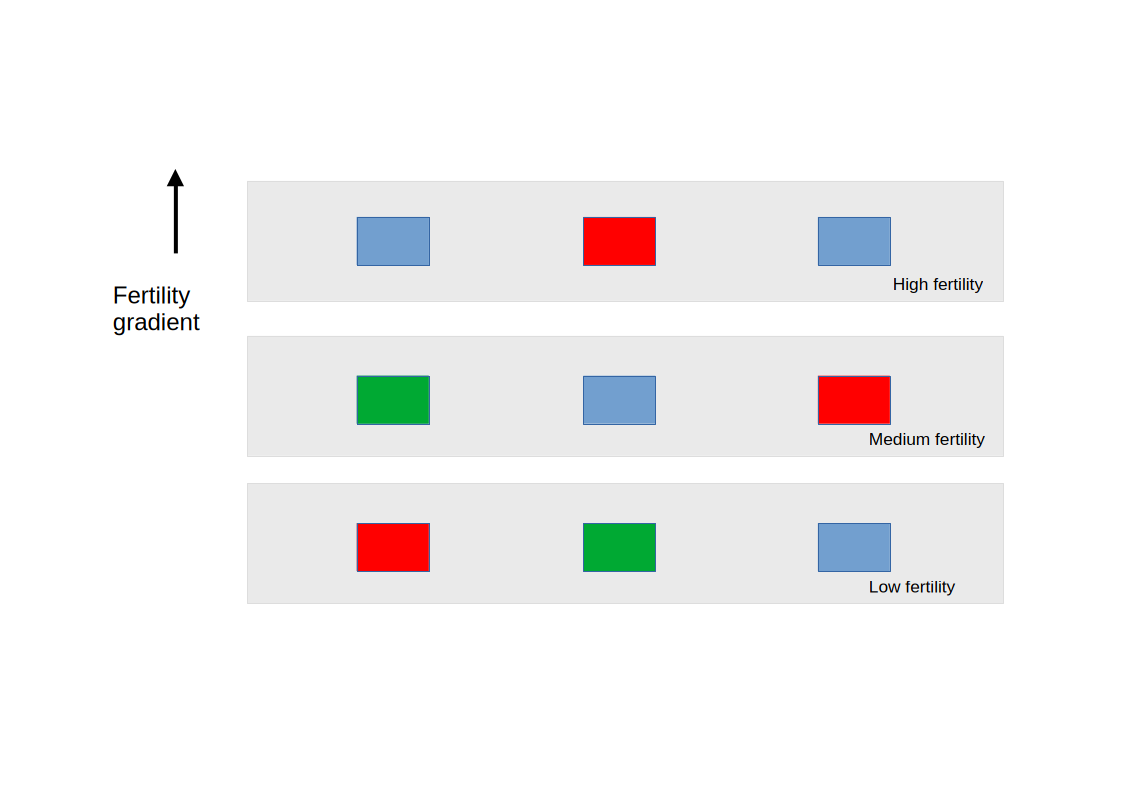
\includegraphics{img/fig2.png}

}

\caption{A randomised complete block design in a field with a
north-south fertility gradient. The field is divided into three blocks
(South, Middle, North) corresponding to low, medium, and high soil
fertility. Within each block, the three treatments are randomly assigned
to plots. The gradient affects all plots equally within a block, so
block-to-block differences can be separated from treatment differences.}

\end{figure}%

The key feature of this design is that every treatment appears exactly
once in every block. Whatever the fertility level of the North block,
all three treatments experience it equally, so the block effect cannot
be confused with the treatment effect.

\subsection{The Treatment Error
Formula}\label{the-treatment-error-formula}

Before seeing the benefit of blocking in numbers, recall what the
treatment error term actually is. In a one-way ANOVA without blocking,
the error mean square is:

\[MS_{\text{error}} = \frac{SS_{\text{error}}}{df_{\text{error}}}
= \frac{\sum_{j=1}^k \sum_{i=1}^{n_j} (y_{ij} - \bar{y}_j)^2}
       {N - k}\]

This pools all sources of uncontrolled variation, including the
fertility gradient, into a single noise estimate. The F ratio for
treatment is:

\[F = \frac{MS_{\text{treatment}}}{MS_{\text{error}}}\]

A large \(MS_{\text{error}}\) makes this ratio smaller and the test less
powerful. Blocking removes the block variation from the numerator of
\(MS_{\text{error}}\), leaving a smaller, cleaner noise estimate:

\[MS_{\text{error (blocked)}} =
\frac{SS_{\text{total}} - SS_{\text{treatment}} - SS_{\text{block}}}
     {(k-1)(b-1)}\]

where \(b\) is the number of blocks. The block sum of squares
\(SS_{\text{block}}\) is extracted from the error, shrinking
\(MS_{\text{error}}\) and therefore increasing the F ratio for the
treatment comparison.

\subsection{Simulating the Field
Experiment}\label{simulating-the-field-experiment}

\begin{Shaded}
\begin{Highlighting}[]
\CommentTok{\# The field data, yields assigned to reflect:}
\CommentTok{\# 1. A real treatment effect (Nitrogen \textgreater{} Phosphorus \textgreater{} Control)}
\CommentTok{\# 2. A strong north{-}south fertility gradient}
\CommentTok{\# 3. Small residual plot{-}to{-}plot noise}

\FunctionTok{set.seed}\NormalTok{(}\DecValTok{42}\NormalTok{)}

\NormalTok{df\_field }\OtherTok{\textless{}{-}} \FunctionTok{data.frame}\NormalTok{(}
  \AttributeTok{block     =} \FunctionTok{factor}\NormalTok{(}\FunctionTok{rep}\NormalTok{(}\FunctionTok{c}\NormalTok{(}\StringTok{"South"}\NormalTok{, }\StringTok{"Middle"}\NormalTok{, }\StringTok{"North"}\NormalTok{),}
                         \AttributeTok{each =} \DecValTok{3}\NormalTok{),}
                     \AttributeTok{levels =} \FunctionTok{c}\NormalTok{(}\StringTok{"South"}\NormalTok{, }\StringTok{"Middle"}\NormalTok{, }\StringTok{"North"}\NormalTok{)),}
  \AttributeTok{treatment =} \FunctionTok{factor}\NormalTok{(}\FunctionTok{c}\NormalTok{(}
    \StringTok{"Control"}\NormalTok{,    }\StringTok{"Nitrogen"}\NormalTok{,   }\StringTok{"Phosphorus"}\NormalTok{,  }\CommentTok{\# South block}
    \StringTok{"Nitrogen"}\NormalTok{,   }\StringTok{"Phosphorus"}\NormalTok{, }\StringTok{"Control"}\NormalTok{,     }\CommentTok{\# Middle block}
    \StringTok{"Phosphorus"}\NormalTok{, }\StringTok{"Control"}\NormalTok{,    }\StringTok{"Nitrogen"}     \CommentTok{\# North block}
\NormalTok{  ), }\AttributeTok{levels =} \FunctionTok{c}\NormalTok{(}\StringTok{"Control"}\NormalTok{, }\StringTok{"Nitrogen"}\NormalTok{, }\StringTok{"Phosphorus"}\NormalTok{)),}
  \CommentTok{\# Block fertility gradient: South = low, North = high}
  \CommentTok{\# adds 0, 8, 16 units to yields within each block}
  \AttributeTok{block\_effect =} \FunctionTok{rep}\NormalTok{(}\FunctionTok{c}\NormalTok{(}\DecValTok{0}\NormalTok{, }\DecValTok{8}\NormalTok{, }\DecValTok{16}\NormalTok{), }\AttributeTok{each =} \DecValTok{3}\NormalTok{),}
  \CommentTok{\# True treatment effects: Control = 0, N = 6, P = 3}
  \AttributeTok{treatment\_effect =} \FunctionTok{c}\NormalTok{(}\DecValTok{0}\NormalTok{, }\DecValTok{6}\NormalTok{, }\DecValTok{3}\NormalTok{,   }\CommentTok{\# South}
                       \DecValTok{6}\NormalTok{, }\DecValTok{3}\NormalTok{, }\DecValTok{0}\NormalTok{,   }\CommentTok{\# Middle}
                       \DecValTok{3}\NormalTok{, }\DecValTok{0}\NormalTok{, }\DecValTok{6}\NormalTok{)   }\CommentTok{\# North}
\NormalTok{)}

\CommentTok{\# Observed yield = grand mean + block effect + treatment effect + noise}
\NormalTok{df\_field}\SpecialCharTok{$}\NormalTok{yield }\OtherTok{\textless{}{-}} \DecValTok{20} \SpecialCharTok{+}
\NormalTok{  df\_field}\SpecialCharTok{$}\NormalTok{block\_effect }\SpecialCharTok{+}
\NormalTok{  df\_field}\SpecialCharTok{$}\NormalTok{treatment\_effect }\SpecialCharTok{+}
  \FunctionTok{round}\NormalTok{(}\FunctionTok{rnorm}\NormalTok{(}\DecValTok{9}\NormalTok{, }\DecValTok{0}\NormalTok{, }\FloatTok{1.2}\NormalTok{), }\DecValTok{1}\NormalTok{)}
\end{Highlighting}
\end{Shaded}

The observed yields are:

\begin{Shaded}
\begin{Highlighting}[]
\FunctionTok{print}\NormalTok{(df\_field[, }\FunctionTok{c}\NormalTok{(}\StringTok{"block"}\NormalTok{, }\StringTok{"treatment"}\NormalTok{, }\StringTok{"yield"}\NormalTok{)])}
\end{Highlighting}
\end{Shaded}

\begin{verbatim}
#>    block  treatment yield
#> 1  South    Control  21.6
#> 2  South   Nitrogen  25.3
#> 3  South Phosphorus  23.4
#> 4 Middle   Nitrogen  34.8
#> 5 Middle Phosphorus  31.5
#> 6 Middle    Control  27.9
#> 7  North Phosphorus  40.8
#> 8  North    Control  35.9
#> 9  North   Nitrogen  44.4
\end{verbatim}

\subsection{Computing the Treatment Error: With and Without
Blocking}\label{computing-the-treatment-error-with-and-without-blocking}

\begin{Shaded}
\begin{Highlighting}[]
\CommentTok{\# {-}{-}{-} Analysis WITHOUT blocking {-}{-}{-}}
\CommentTok{\# All variation not explained by treatment goes into the error}
\NormalTok{fit\_no\_block }\OtherTok{\textless{}{-}} \FunctionTok{aov}\NormalTok{(yield }\SpecialCharTok{\textasciitilde{}}\NormalTok{ treatment, }\AttributeTok{data =}\NormalTok{ df\_field)}

\NormalTok{ss\_treat\_nb  }\OtherTok{\textless{}{-}} \FunctionTok{summary}\NormalTok{(fit\_no\_block)[[}\DecValTok{1}\NormalTok{]][}\StringTok{"treatment"}\NormalTok{, }\StringTok{"Sum Sq"}\NormalTok{]}
\NormalTok{ss\_error\_nb  }\OtherTok{\textless{}{-}} \FunctionTok{summary}\NormalTok{(fit\_no\_block)[[}\DecValTok{1}\NormalTok{]][}\StringTok{"Residuals"}\NormalTok{, }\StringTok{"Sum Sq"}\NormalTok{]}
\NormalTok{df\_error\_nb  }\OtherTok{\textless{}{-}} \FunctionTok{summary}\NormalTok{(fit\_no\_block)[[}\DecValTok{1}\NormalTok{]][}\StringTok{"Residuals"}\NormalTok{, }\StringTok{"Df"}\NormalTok{]}
\NormalTok{ms\_error\_nb  }\OtherTok{\textless{}{-}}\NormalTok{ ss\_error\_nb }\SpecialCharTok{/}\NormalTok{ df\_error\_nb}
\NormalTok{f\_nb }\OtherTok{\textless{}{-}} \FunctionTok{summary}\NormalTok{(fit\_no\_block)[[}\DecValTok{1}\NormalTok{]][}\StringTok{"treatment"}\NormalTok{, }\StringTok{"F value"}\NormalTok{]}
\NormalTok{p\_nb }\OtherTok{\textless{}{-}} \FunctionTok{summary}\NormalTok{(fit\_no\_block)[[}\DecValTok{1}\NormalTok{]][}\StringTok{"treatment"}\NormalTok{, }\StringTok{"Pr(\textgreater{}F)"}\NormalTok{]}

\CommentTok{\# {-}{-}{-} Analysis WITH blocking {-}{-}{-}}
\CommentTok{\# Block variation is extracted from the error}
\NormalTok{fit\_blocked  }\OtherTok{\textless{}{-}} \FunctionTok{aov}\NormalTok{(yield }\SpecialCharTok{\textasciitilde{}}\NormalTok{ treatment }\SpecialCharTok{+}\NormalTok{ block, }\AttributeTok{data =}\NormalTok{ df\_field)}

\NormalTok{ss\_treat\_b   }\OtherTok{\textless{}{-}} \FunctionTok{summary}\NormalTok{(fit\_blocked)[[}\DecValTok{1}\NormalTok{]][}\StringTok{"treatment"}\NormalTok{, }\StringTok{"Sum Sq"}\NormalTok{]}
\NormalTok{ss\_block     }\OtherTok{\textless{}{-}} \FunctionTok{summary}\NormalTok{(fit\_blocked)[[}\DecValTok{1}\NormalTok{]][}\StringTok{"block"}\NormalTok{,     }\StringTok{"Sum Sq"}\NormalTok{]}
\NormalTok{ss\_error\_b   }\OtherTok{\textless{}{-}} \FunctionTok{summary}\NormalTok{(fit\_blocked)[[}\DecValTok{1}\NormalTok{]][}\StringTok{"Residuals"}\NormalTok{, }\StringTok{"Sum Sq"}\NormalTok{]}
\NormalTok{df\_error\_b   }\OtherTok{\textless{}{-}} \FunctionTok{summary}\NormalTok{(fit\_blocked)[[}\DecValTok{1}\NormalTok{]][}\StringTok{"Residuals"}\NormalTok{, }\StringTok{"Df"}\NormalTok{]}
\NormalTok{ms\_error\_b   }\OtherTok{\textless{}{-}}\NormalTok{ ss\_error\_b }\SpecialCharTok{/}\NormalTok{ df\_error\_b}
\NormalTok{f\_b }\OtherTok{\textless{}{-}} \FunctionTok{summary}\NormalTok{(fit\_blocked)[[}\DecValTok{1}\NormalTok{]][}\StringTok{"treatment"}\NormalTok{, }\StringTok{"F value"}\NormalTok{]}
\NormalTok{p\_b }\OtherTok{\textless{}{-}} \FunctionTok{summary}\NormalTok{(fit\_blocked)[[}\DecValTok{1}\NormalTok{]][}\StringTok{"treatment"}\NormalTok{, }\StringTok{"Pr(\textgreater{}F)"}\NormalTok{]}
\end{Highlighting}
\end{Shaded}

\begin{Shaded}
\begin{Highlighting}[]
\CommentTok{\# cache: true}
\FunctionTok{cat}\NormalTok{(}
  \StringTok{"=== WITHOUT blocking ===}\SpecialCharTok{\textbackslash{}n}\StringTok{SS treatment: "}\NormalTok{,}
  \FunctionTok{round}\NormalTok{(ss\_treat\_nb, }\DecValTok{2}\NormalTok{), }
  \StringTok{"}\SpecialCharTok{\textbackslash{}n}\StringTok{SS error:"}\NormalTok{, }\FunctionTok{round}\NormalTok{(ss\_error\_nb, }\DecValTok{2}\NormalTok{),}
  \StringTok{"(includes block gradient)}\SpecialCharTok{\textbackslash{}n}\StringTok{df error:"}\NormalTok{,}
\NormalTok{  df\_error\_nb, }\StringTok{"}\SpecialCharTok{\textbackslash{}n}\StringTok{MS error:"}\NormalTok{,}
  \FunctionTok{round}\NormalTok{(ms\_error\_nb, }\DecValTok{2}\NormalTok{), }\StringTok{"}\SpecialCharTok{\textbackslash{}n}\StringTok{F value:"}\NormalTok{, }
  \FunctionTok{round}\NormalTok{(f\_nb, }\DecValTok{3}\NormalTok{), }\StringTok{"}\SpecialCharTok{\textbackslash{}n}\StringTok{p{-}value:"}\NormalTok{, }\FunctionTok{round}\NormalTok{(p\_nb, }\DecValTok{3}\NormalTok{), }\StringTok{"}\SpecialCharTok{\textbackslash{}n\textbackslash{}n}\StringTok{"}\NormalTok{)}
\end{Highlighting}
\end{Shaded}

\begin{verbatim}
#> === WITHOUT blocking ===
#> SS treatment:  60.93 
#> SS error: 436.75 (includes block gradient)
#> df error: 6 
#> MS error: 72.79 
#> F value: 0.418 
#> p-value: 0.676
\end{verbatim}

\begin{Shaded}
\begin{Highlighting}[]
\FunctionTok{cat}\NormalTok{(}
  \StringTok{"=== WITH blocking ===}\SpecialCharTok{\textbackslash{}n}\StringTok{SS treatment: "}\NormalTok{,}
  \FunctionTok{round}\NormalTok{(ss\_treat\_b, }\DecValTok{2}\NormalTok{),}
  \StringTok{"}\SpecialCharTok{\textbackslash{}n}\StringTok{SS block:"}\NormalTok{, }\FunctionTok{round}\NormalTok{(ss\_block, }\DecValTok{2}\NormalTok{),}
  \StringTok{"(extracted from error)}\SpecialCharTok{\textbackslash{}n}\StringTok{SS error:"}\NormalTok{,}
  \FunctionTok{round}\NormalTok{(ss\_error\_b, }\DecValTok{2}\NormalTok{),}
  \StringTok{"(block gradient removed)}\SpecialCharTok{\textbackslash{}n}\StringTok{df error:"}\NormalTok{,}
\NormalTok{  df\_error\_b, }\StringTok{"}\SpecialCharTok{\textbackslash{}n}\StringTok{MS error:"}\NormalTok{,}
  \FunctionTok{round}\NormalTok{(ms\_error\_b, }\DecValTok{2}\NormalTok{),}
  \StringTok{"}\SpecialCharTok{\textbackslash{}n}\StringTok{F value:"}\NormalTok{, }\FunctionTok{round}\NormalTok{(f\_b, }\DecValTok{3}\NormalTok{),}
  \StringTok{"}\SpecialCharTok{\textbackslash{}n}\StringTok{p{-}value:"}\NormalTok{, }\FunctionTok{round}\NormalTok{(p\_b,  }\DecValTok{3}\NormalTok{), }\StringTok{"}\SpecialCharTok{\textbackslash{}n\textbackslash{}n}\StringTok{"}\NormalTok{)}
\end{Highlighting}
\end{Shaded}

\begin{verbatim}
#> === WITH blocking ===
#> SS treatment:  60.93 
#> SS block: 430.61 (extracted from error)
#> SS error: 6.15 (block gradient removed)
#> df error: 4 
#> MS error: 1.54 
#> F value: 19.824 
#> p-value: 0.008
\end{verbatim}

\begin{Shaded}
\begin{Highlighting}[]
\FunctionTok{cat}\NormalTok{(}
  \StringTok{"=== Summary ===}\SpecialCharTok{\textbackslash{}n}\StringTok{MS error reduced from"}\NormalTok{,}
  \FunctionTok{round}\NormalTok{(ms\_error\_nb, }\DecValTok{2}\NormalTok{), }\StringTok{"to"}\NormalTok{, }
  \FunctionTok{round}\NormalTok{(ms\_error\_b, }\DecValTok{2}\NormalTok{), }
  \StringTok{"by blocking}\SpecialCharTok{\textbackslash{}n}\StringTok{F value increased from"}\NormalTok{, }
  \FunctionTok{round}\NormalTok{(f\_nb, }\DecValTok{3}\NormalTok{), }\StringTok{"to"}\NormalTok{, }\FunctionTok{round}\NormalTok{(f\_b, }\DecValTok{3}\NormalTok{), }\StringTok{"}\SpecialCharTok{\textbackslash{}n}\StringTok{"}\NormalTok{)}
\end{Highlighting}
\end{Shaded}

\begin{verbatim}
#> === Summary ===
#> MS error reduced from 72.79 to 1.54 by blocking
#> F value increased from 0.418 to 19.824
\end{verbatim}

The two analyses use identical data, the same nine yield observations
from the same nine plots. The only difference is whether the block
structure is accounted for in the model.

Without blocking, the \(SS_{\text{error}}\) includes both the genuine
residual plot noise and the large fertility gradient running from south
to north. This inflates \(MS_{\text{error}}\), shrinks the F ratio, and
makes the treatment differences harder to detect.

With blocking, the \(SS_{\text{block}}\) is extracted from what would
otherwise be the error. The \(SS_{\text{error}}\) now contains only the
genuine residual noise --- the small, uncontrollable plot-to-plot
differences that remain after removing both the treatment effect and the
block gradient. The \(MS_{\text{error}}\) drops substantially, the F
ratio rises, and the p-value falls --- not because the data have
changed, but because the analysis is now asking the right question: do
treatments differ after accounting for the known gradient?

This is the mechanical benefit of blocking stated precisely: it moves
known variation out of the error term, leaving a cleaner and smaller
noise estimate against which the treatment effect is judged.

\subsection{Reading the Numbers}\label{reading-the-numbers}

The two analyses use identical data, the same nine yield observations
from the same nine plots. The only difference is whether the block
structure is accounted for in the model, and the consequences are
dramatic.

\textbf{Without blocking}, \(SS_{\text{error}} = 436.75\) against a
\(SS_{\text{treatment}} = 60.93\). The error sum of squares is more than
seven times larger than the treatment sum of squares because it contains
the entire north-south fertility gradient, 430 units worth of variation
that has nothing to do with fertiliser but is lumped into the noise. The
resulting \(MS_{\text{error}} = 72.79\) overwhelms the treatment signal,
producing \(F_{2,6} = 0.418\) and \(p = 0.676\). A researcher using this
analysis would conclude that fertiliser has no detectable effect which
would be a false negative caused entirely by a preventable design flaw.

\textbf{With blocking}, the picture reverses completely.
\(SS_{\text{block}} = 430.61\) is extracted from the error and placed in
its own term, this is the fertility gradient, accounted for and set
aside. What remains in \(SS_{\text{error}}\) is only \(6.15\): the
genuine plot-to-plot residual noise after removing both the treatment
effect and the gradient. \(MS_{\text{error}}\) drops from 72.79 to 1.54,
a 47-fold reduction, and the \(F\) ratio climbs from 0.418 to
\(F_{2,4} = 19.82\), with \(p = 0.008\).

The \(SS_{\text{treatment}}\) is identical in both analyses, 60.93 in
both cases. The treatment effect in the data has not changed. What
changed is the denominator of the F ratio: by removing the gradient from
the error term, the analysis can finally hear the treatment signal above
the noise.

Two additional details are worth noting. First, the blocked analysis has
fewer error degrees of freedom (\(df = 4\) instead of \(df = 6\))
because two degrees of freedom were spent estimating the block effects.
Despite this loss, the test is far more powerful which is a direct
consequence of the enormous reduction in \(MS_{\text{error}}\). Second,
this example is not contrived: a fertility gradient with
\(SS_{\text{block}} = 430\) versus a residual of
\(SS_{\text{error}} = 6\) is entirely realistic in agricultural and
ecological field experiments. Gradients of this magnitude are common,
which is precisely why blocking has been standard practice in field
experimentation since Fisher's time at Rothamsted.

The practical lesson is unambiguous: \textbf{if you know a gradient
exists, block on it before you randomise.} Failing to do so does not
just reduce power, as these numbers show, it can make a real and
substantial treatment effect completely invisible.

\subsection{When to Block}\label{when-to-block}

Block when there is a known, measurable source of variation that will
affect the response but is not the treatment of interest. Common
blocking factors in biology include:

\begin{itemize}
\tightlist
\item
  \textbf{Spatial position}: location in a greenhouse, field, or
  laboratory bench.
\item
  \textbf{Temporal batches}: animals processed on different days, assays
  run in different batches, samples collected in different seasons.
\item
  \textbf{Individual characteristics}: litters in animal experiments,
  maternal plants in seed studies, patients recruited from different
  centres.
\end{itemize}

Do not block on variables that are themselves affected by the treatment
as this introduces bias. And do not block on a variable that is
unrelated to the response: adding an irrelevant block factor costs
degrees of freedom from the error term and can actually reduce power.

\section{Designing for the ANOVA You Want to
Run}\label{designing-for-the-anova-you-want-to-run}

\subsection{Start With the Analysis}\label{start-with-the-analysis}

The most common design error in biology is designing an experiment
without thinking about how it will be analysed. The design and the
analysis are not separate activities, they are two sides of the same
coin. Every feature of the design has a direct counterpart in the
statistical model, and mismatches between design and analysis are the
primary source of invalid inference.

The practical discipline is to write the analysis plan, including the
model formula (in R), before collecting any data:

\begin{Shaded}
\begin{Highlighting}[]
\CommentTok{\# Write your intended model formula before data collection}
\CommentTok{\# One{-}way ANOVA}
\FunctionTok{aov}\NormalTok{(response }\SpecialCharTok{\textasciitilde{}}\NormalTok{ treatment, }\AttributeTok{data =}\NormalTok{ df)}

\CommentTok{\# Randomised complete block design}
\FunctionTok{aov}\NormalTok{(response }\SpecialCharTok{\textasciitilde{}}\NormalTok{ treatment }\SpecialCharTok{+}\NormalTok{ block, }\AttributeTok{data =}\NormalTok{ df)}

\CommentTok{\# Two{-}way factorial}
\FunctionTok{aov}\NormalTok{(response }\SpecialCharTok{\textasciitilde{}}\NormalTok{ factorA }\SpecialCharTok{*}\NormalTok{ factorB, }\AttributeTok{data =}\NormalTok{ df)}

\CommentTok{\# Split{-}plot}
\FunctionTok{aov}\NormalTok{(response }\SpecialCharTok{\textasciitilde{}}\NormalTok{ whole\_plot\_factor }\SpecialCharTok{*}\NormalTok{ subplot\_factor }\SpecialCharTok{+}
      \FunctionTok{Error}\NormalTok{(whole\_plot\_unit }\SpecialCharTok{/}\NormalTok{ subplot\_factor), }\AttributeTok{data =}\NormalTok{ df)}

\CommentTok{\# Repeated measures}
\NormalTok{lmerTest}\SpecialCharTok{::}\FunctionTok{lmer}\NormalTok{(response }\SpecialCharTok{\textasciitilde{}}\NormalTok{ treatment }\SpecialCharTok{*}\NormalTok{ time }\SpecialCharTok{+}\NormalTok{ (}\DecValTok{1} \SpecialCharTok{|}\NormalTok{ subject),}
               \AttributeTok{data =}\NormalTok{ df)}

\CommentTok{\# Nested design}
\FunctionTok{aov}\NormalTok{(response }\SpecialCharTok{\textasciitilde{}}\NormalTok{ treatment }\SpecialCharTok{+} \FunctionTok{Error}\NormalTok{(block }\SpecialCharTok{/}\NormalTok{ subplot), }\AttributeTok{data =}\NormalTok{ df)}
\end{Highlighting}
\end{Shaded}

Writing the formula in advance forces you to identify the experimental
unit, the error term, and the random effects structure before the data
are collected. If you cannot write the formula, the design is not yet
fully specified.

\subsection{Match the Unit of Analysis to the Unit of
Randomisation}\label{match-the-unit-of-analysis-to-the-unit-of-randomisation}

The experimental unit, the entity that received the treatment
independently, must be the unit of analysis. This principle, stated
simply, prevents most cases of pseudoreplication.

A decision tree for identifying the experimental unit:

\begin{itemize}
\tightlist
\item
  What was randomly assigned to receive the treatment?
\item
  Could two observations have received different treatments? If no, they
  are from the same experimental unit.
\item
  Is the treatment applied to groups of individuals, or to individuals
  separately?
\end{itemize}

\begin{Shaded}
\begin{Highlighting}[]
\CommentTok{\# Example 1: Correct, individual plants randomised to treatment}
\CommentTok{\# Experimental unit = plant, n = 20 per treatment}
\NormalTok{df\_correct }\OtherTok{\textless{}{-}} \FunctionTok{data.frame}\NormalTok{(}
  \AttributeTok{yield     =} \FunctionTok{rnorm}\NormalTok{(}\DecValTok{60}\NormalTok{, }\AttributeTok{mean =} \DecValTok{20}\NormalTok{, }\AttributeTok{sd =} \DecValTok{3}\NormalTok{),}
  \AttributeTok{treatment =} \FunctionTok{rep}\NormalTok{(}\FunctionTok{c}\NormalTok{(}\StringTok{"A"}\NormalTok{, }\StringTok{"B"}\NormalTok{, }\StringTok{"C"}\NormalTok{), }\AttributeTok{each =} \DecValTok{20}\NormalTok{),}
  \AttributeTok{plant     =} \DecValTok{1}\SpecialCharTok{:}\DecValTok{60}
\NormalTok{)}
\CommentTok{\# Correct analysis: plant is the unit}
\FunctionTok{summary}\NormalTok{(}\FunctionTok{aov}\NormalTok{(yield }\SpecialCharTok{\textasciitilde{}}\NormalTok{ treatment, }\AttributeTok{data =}\NormalTok{ df\_correct))}
\end{Highlighting}
\end{Shaded}

\begin{verbatim}
#>             Df Sum Sq Mean Sq F value Pr(>F)
#> treatment    2   28.2   14.12   1.234  0.299
#> Residuals   57  652.1   11.44
\end{verbatim}

\begin{Shaded}
\begin{Highlighting}[]
\CommentTok{\# Example 2: Wrong, treatment applied to cages,}
\CommentTok{\# multiple animals measured per cage}
\CommentTok{\# Experimental unit = cage (n = 4 per treatment),}
\CommentTok{\# not animal (n = 20 per treatment)}
\FunctionTok{set.seed}\NormalTok{(}\DecValTok{42}\NormalTok{)}
\NormalTok{cage\_effect }\OtherTok{\textless{}{-}} \FunctionTok{rnorm}\NormalTok{(}\DecValTok{12}\NormalTok{, }\DecValTok{0}\NormalTok{, }\DecValTok{2}\NormalTok{)   }\CommentTok{\# 4 cages per treatment}
\NormalTok{df\_pseudo   }\OtherTok{\textless{}{-}} \FunctionTok{data.frame}\NormalTok{(}
  \AttributeTok{weight    =} \FunctionTok{c}\NormalTok{(}\FunctionTok{sapply}\NormalTok{(}\DecValTok{1}\SpecialCharTok{:}\DecValTok{12}\NormalTok{, }\ControlFlowTok{function}\NormalTok{(c) \{}
    \FunctionTok{rnorm}\NormalTok{(}\DecValTok{5}\NormalTok{, }\AttributeTok{mean =} \DecValTok{20} \SpecialCharTok{+}\NormalTok{ cage\_effect[c], }\AttributeTok{sd =} \FloatTok{0.5}\NormalTok{)}
\NormalTok{  \})),}
  \AttributeTok{treatment =} \FunctionTok{rep}\NormalTok{(}\FunctionTok{rep}\NormalTok{(}\FunctionTok{c}\NormalTok{(}\StringTok{"A"}\NormalTok{, }\StringTok{"B"}\NormalTok{, }\StringTok{"C"}\NormalTok{), }\AttributeTok{each =} \DecValTok{4}\NormalTok{), }\AttributeTok{each =} \DecValTok{5}\NormalTok{),}
  \AttributeTok{cage      =} \FunctionTok{rep}\NormalTok{(}\DecValTok{1}\SpecialCharTok{:}\DecValTok{12}\NormalTok{, }\AttributeTok{each =} \DecValTok{5}\NormalTok{)}
\NormalTok{)}

\CommentTok{\# Wrong: treats animals as independent}
\NormalTok{wrong\_fit }\OtherTok{\textless{}{-}} \FunctionTok{aov}\NormalTok{(weight }\SpecialCharTok{\textasciitilde{}}\NormalTok{ treatment, }\AttributeTok{data =}\NormalTok{ df\_pseudo)}
\FunctionTok{cat}\NormalTok{(}\StringTok{"Wrong analysis df (error):"}\NormalTok{,}
    \FunctionTok{summary}\NormalTok{(wrong\_fit)[[}\DecValTok{1}\NormalTok{]][}\StringTok{"Residuals"}\NormalTok{, }\StringTok{"Df"}\NormalTok{], }\StringTok{"}\SpecialCharTok{\textbackslash{}n}\StringTok{"}\NormalTok{)}
\end{Highlighting}
\end{Shaded}

\begin{verbatim}
#> Wrong analysis df (error): 57
\end{verbatim}

\begin{Shaded}
\begin{Highlighting}[]
\CommentTok{\# Correct: uses cage means}
\NormalTok{cage\_means }\OtherTok{\textless{}{-}} \FunctionTok{aggregate}\NormalTok{(weight }\SpecialCharTok{\textasciitilde{}}\NormalTok{ treatment }\SpecialCharTok{+}\NormalTok{ cage,}
                         \AttributeTok{data =}\NormalTok{ df\_pseudo, }\AttributeTok{FUN =}\NormalTok{ mean)}
\NormalTok{correct\_fit }\OtherTok{\textless{}{-}} \FunctionTok{aov}\NormalTok{(weight }\SpecialCharTok{\textasciitilde{}}\NormalTok{ treatment, }\AttributeTok{data =}\NormalTok{ cage\_means)}
\FunctionTok{cat}\NormalTok{(}\StringTok{"Correct analysis df (error):"}\NormalTok{,}
    \FunctionTok{summary}\NormalTok{(correct\_fit)[[}\DecValTok{1}\NormalTok{]][}\StringTok{"Residuals"}\NormalTok{, }\StringTok{"Df"}\NormalTok{], }\StringTok{"}\SpecialCharTok{\textbackslash{}n}\StringTok{"}\NormalTok{)}
\end{Highlighting}
\end{Shaded}

\begin{verbatim}
#> Correct analysis df (error): 9
\end{verbatim}

\subsection{Anticipate the Covariance
Structure}\label{anticipate-the-covariance-structure}

If the design involves repeated measurements, nested units, or crossed
random effects, specify the covariance structure before data collection
and verify that the intended model is identifiable given the planned
sample sizes. A three-level nested model requires sufficient replication
at every level, and ``sufficient'' means at least 3-4 units per level
for variance components to be estimated at all, and ideally 10-15 for
reliable estimation.

\section{Common Design Mistakes in Biology and How to Avoid
Them}\label{common-design-mistakes-in-biology-and-how-to-avoid-them}

\subsection{Mistake 1:
Pseudoreplication}\label{mistake-1-pseudoreplication}

Already covered in depth in sections \ref{sec-pseudoreplication} and
\ref{sec-pseudoreplication2}, but worth restating as a design principle:
\textbf{never confuse the unit of measurement with the unit of
replication.} The most reliable protection is to draw the hierarchy
explicitly before data collection (fields contain plots contain plants)
and verify that the treatment is randomised at the level you intend to
analyse.

\subsection{Mistake 2: Confounding Treatment With a Nuisance
Variable}\label{mistake-2-confounding-treatment-with-a-nuisance-variable}

Confounding occurs when a nuisance variable is systematically associated
with the treatment, making it impossible to separate their effects. The
classic example: all control pots placed on the north bench and all
nitrogen pots placed on the south bench. Any observed difference in
yield now conflates the treatment effect with the bench position effect.

The remedy is randomisation, but randomisation must be applied at the
right level and genuinely implemented:

\begin{Shaded}
\begin{Highlighting}[]
\FunctionTok{library}\NormalTok{(ggplot2)}
\FunctionTok{library}\NormalTok{(patchwork)}

\CommentTok{\# Confounded design}
\NormalTok{df\_confounded }\OtherTok{\textless{}{-}} \FunctionTok{data.frame}\NormalTok{(}
  \AttributeTok{yield     =} \FunctionTok{c}\NormalTok{(}\FunctionTok{rnorm}\NormalTok{(}\DecValTok{10}\NormalTok{, }\AttributeTok{mean =} \DecValTok{18}\NormalTok{, }\AttributeTok{sd =} \DecValTok{2}\NormalTok{),  }\CommentTok{\# Control, shaded}
                \FunctionTok{rnorm}\NormalTok{(}\DecValTok{10}\NormalTok{, }\AttributeTok{mean =} \DecValTok{24}\NormalTok{, }\AttributeTok{sd =} \DecValTok{2}\NormalTok{)),  }\CommentTok{\# Nitrogen, sunny}
  \AttributeTok{treatment =} \FunctionTok{rep}\NormalTok{(}\FunctionTok{c}\NormalTok{(}\StringTok{"Control"}\NormalTok{, }\StringTok{"Nitrogen"}\NormalTok{), }\AttributeTok{each =} \DecValTok{10}\NormalTok{),}
  \AttributeTok{position  =} \FunctionTok{rep}\NormalTok{(}\FunctionTok{c}\NormalTok{(}\StringTok{"Shaded"}\NormalTok{, }\StringTok{"Sunny"}\NormalTok{), }\AttributeTok{each =} \DecValTok{10}\NormalTok{)}
\NormalTok{)}

\CommentTok{\# Randomised design}
\NormalTok{df\_randomised }\OtherTok{\textless{}{-}} \FunctionTok{data.frame}\NormalTok{(}
  \AttributeTok{yield     =} \FunctionTok{c}\NormalTok{(}\FunctionTok{rnorm}\NormalTok{(}\DecValTok{10}\NormalTok{, }\AttributeTok{mean =} \DecValTok{20}\NormalTok{, }\AttributeTok{sd =} \DecValTok{2}\NormalTok{),  }\CommentTok{\# Control, mixed}
                \FunctionTok{rnorm}\NormalTok{(}\DecValTok{10}\NormalTok{, }\AttributeTok{mean =} \DecValTok{24}\NormalTok{, }\AttributeTok{sd =} \DecValTok{2}\NormalTok{)),  }\CommentTok{\# Nitrogen, mixed}
  \AttributeTok{treatment =} \FunctionTok{rep}\NormalTok{(}\FunctionTok{c}\NormalTok{(}\StringTok{"Control"}\NormalTok{, }\StringTok{"Nitrogen"}\NormalTok{), }\AttributeTok{each =} \DecValTok{10}\NormalTok{),}
  \AttributeTok{position  =} \FunctionTok{sample}\NormalTok{(}\FunctionTok{rep}\NormalTok{(}\FunctionTok{c}\NormalTok{(}\StringTok{"Shaded"}\NormalTok{, }\StringTok{"Sunny"}\NormalTok{), }\DecValTok{10}\NormalTok{))}
\NormalTok{)}

\NormalTok{p1 }\OtherTok{\textless{}{-}} \FunctionTok{ggplot}\NormalTok{(df\_confounded,}
             \FunctionTok{aes}\NormalTok{(}\AttributeTok{x =}\NormalTok{ treatment, }\AttributeTok{y =}\NormalTok{ yield,}
                 \AttributeTok{colour =}\NormalTok{ position, }\AttributeTok{shape =}\NormalTok{ position)) }\SpecialCharTok{+}
  \FunctionTok{geom\_jitter}\NormalTok{(}\AttributeTok{width =} \FloatTok{0.1}\NormalTok{, }\AttributeTok{size =} \DecValTok{3}\NormalTok{, }\AttributeTok{alpha =} \FloatTok{0.8}\NormalTok{) }\SpecialCharTok{+}
  \FunctionTok{scale\_colour\_manual}\NormalTok{(}\AttributeTok{values =} \FunctionTok{c}\NormalTok{(}\StringTok{"\#2E86AB"}\NormalTok{, }\StringTok{"\#F6AE2D"}\NormalTok{)) }\SpecialCharTok{+}
  \FunctionTok{labs}\NormalTok{(}\AttributeTok{title    =} \StringTok{"Confounded design"}\NormalTok{,}
       \AttributeTok{subtitle =} \StringTok{"Treatment perfectly correlated with position"}\NormalTok{,}
       \AttributeTok{x =} \ConstantTok{NULL}\NormalTok{, }\AttributeTok{y =} \StringTok{"Yield"}\NormalTok{,}
       \AttributeTok{colour =} \StringTok{"Position"}\NormalTok{, }\AttributeTok{shape =} \StringTok{"Position"}\NormalTok{) }\SpecialCharTok{+}
  \FunctionTok{theme\_bw}\NormalTok{()}

\NormalTok{p2 }\OtherTok{\textless{}{-}} \FunctionTok{ggplot}\NormalTok{(df\_randomised,}
             \FunctionTok{aes}\NormalTok{(}\AttributeTok{x =}\NormalTok{ treatment, }\AttributeTok{y =}\NormalTok{ yield,}
                 \AttributeTok{colour =}\NormalTok{ position, }\AttributeTok{shape =}\NormalTok{ position)) }\SpecialCharTok{+}
  \FunctionTok{geom\_jitter}\NormalTok{(}\AttributeTok{width =} \FloatTok{0.1}\NormalTok{, }\AttributeTok{size =} \DecValTok{3}\NormalTok{, }\AttributeTok{alpha =} \FloatTok{0.8}\NormalTok{) }\SpecialCharTok{+}
  \FunctionTok{scale\_colour\_manual}\NormalTok{(}\AttributeTok{values =} \FunctionTok{c}\NormalTok{(}\StringTok{"\#2E86AB"}\NormalTok{, }\StringTok{"\#F6AE2D"}\NormalTok{)) }\SpecialCharTok{+}
  \FunctionTok{labs}\NormalTok{(}\AttributeTok{title    =} \StringTok{"Randomised design"}\NormalTok{,}
       \AttributeTok{subtitle =} \StringTok{"Both positions represented in both treatments"}\NormalTok{,}
       \AttributeTok{x =} \ConstantTok{NULL}\NormalTok{, }\AttributeTok{y =} \StringTok{"Yield"}\NormalTok{,}
       \AttributeTok{colour =} \StringTok{"Position"}\NormalTok{, }\AttributeTok{shape =} \StringTok{"Position"}\NormalTok{) }\SpecialCharTok{+}
  \FunctionTok{theme\_bw}\NormalTok{()}

\NormalTok{p1 }\SpecialCharTok{+}\NormalTok{ p2}
\end{Highlighting}
\end{Shaded}

\begin{figure}[H]

\centering{

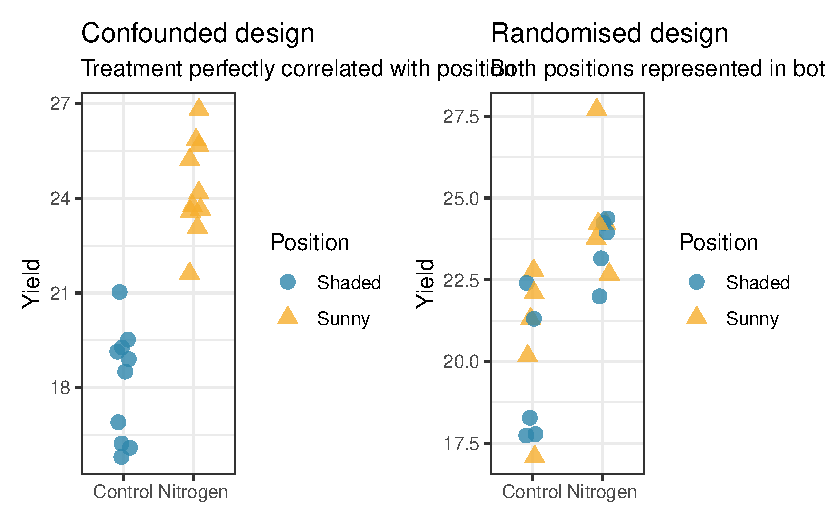
\includegraphics[width=0.9\textwidth,height=\textheight]{05a-experimental-design_files/figure-pdf/fig-confounding-demo-1.pdf}

}

\caption{\label{fig-confounding-demo}Confounding illustrated. Left: a
confounded design where all Control plants are on the shaded side of the
greenhouse and all Nitrogen plants are on the sunny side. Any observed
difference conflates treatment with light availability. Right: a
properly randomised design where both treatments are represented on both
sides, eliminating the confound.}

\end{figure}%

\subsection{Mistake 3: Insufficient Replication at the Right
Level}\label{mistake-3-insufficient-replication-at-the-right-level}

Researchers sometimes add subsamples to increase apparent sample size
without adding true replication. Five soil cores per plot does not give
you five replicates: it gives you one plot measured five times. The
number that matters for the treatment comparison is the number of
independently treated plots, not the number of measurements per plot.

The consequence is not merely conservative, it is incorrect. As Sections
\ref{sec-pseudoreplication} and \ref{sec-pseudoreplication2}
demonstrated, treating subsamples as replicates can inflate the false
positive rate to 25\% or higher.

A practical check: if you removed four of your five subsamples per plot,
would you lose replication for the treatment comparison? If no (if the
treatment comparison is still based on the same number of plots) the
subsamples are providing precision within plots, not replication for
treatments.

\subsection{Mistake 4: Unbalanced Designs by
Negligence}\label{mistake-4-unbalanced-designs-by-negligence}

Some imbalance is inevitable, animals die, samples are lost, patients
drop out. But imbalance that arises from avoidable causes, not
randomising properly, not accounting for expected dropout or not
over-recruiting to compensate, creates unnecessary analytical
complications (Section \ref{sec-unbalanced}) and reduces power.

The practical remedy is simple: \textbf{over-recruit by 10-20\% per
cell} when dropout or loss is anticipated, and document the expected
attrition rate in the analysis plan. If dropout is systematic rather
than random, sicker patients are more likely to drop out, the resulting
missing data problem cannot be solved by over-recruiting and requires
explicit handling in the analysis.

\subsection{Mistake 5: Measuring the Wrong Response
Variable}\label{mistake-5-measuring-the-wrong-response-variable}

Choosing a response variable that is insensitive to the treatment, or
that is measured too imprecisely, undermines the experiment regardless
of how well it is designed. Two principles apply.

\textbf{Measure as close to the biological process of interest as
possible.} If you want to know whether a drug reduces inflammation,
measure the inflammatory marker directly, not a distal outcome that may
be affected by many other factors.

\textbf{Use the most precise measurement available within practical
constraints.} A continuous measurement (tumour volume in mm³) is almost
always more informative than a binary one (tumour present/absent), and
requires a smaller sample size to achieve the same power.

\subsection{Mistake 6: Ignoring the Temporal
Structure}\label{mistake-6-ignoring-the-temporal-structure}

In longitudinal studies, the order of measurements matters.
Pre-treatment baseline measurements are not the same as post-treatment
measurements, and treating all time points as exchangeable, as if the
order were arbitrary, discards information and can introduce bias.

The correct approach is to use the baseline measurement as a covariate
(ANCOVA) or to model time explicitly as a within-subject factor
(repeated measures ANOVA or mixed model). Either approach extracts more
information from the data than ignoring the temporal structure.

\section{Sample Size and Power Before the Experiment, Not
After}\label{sec-sample-size-power}

\subsection{Power Analysis Is a Professional
Obligation}\label{power-analysis-is-a-professional-obligation}

Power analysis was introduced in Section 3.4 in the context of one-way
ANOVA. Here we revisit it as a design principle that applies to every
experiment in this book, not just one-way ANOVA.

Running an underpowered experiment is not merely a missed opportunity,
it is a waste of resources, animal lives, or patient time, and it
produces results that cannot be trusted. A non-significant result from
an underpowered study tells you almost nothing: the effect might be
absent, or it might be real but too small for the study to detect. These
two conclusions are not the same, and conflating them has contributed
significantly to the replication crisis in biological research.

Power analysis before the experiment forces you to commit to:

\begin{enumerate}
\def\labelenumi{\arabic{enumi}.}
\tightlist
\item
  A specific effect size of scientific interest.
\item
  A sample size that gives adequate power to detect it.
\item
  A significance threshold you will use for the analysis.
\end{enumerate}

All three must be specified before data collection. Adjusting them after
seeing the data, stopping early because the result is significant, or
continuing because it is not, invalidates the analysis.

\subsection{Power for Common Designs}\label{power-for-common-designs}

The \texttt{pwr} package handles power analysis for standard ANOVA
designs. For mixed models and GLMMs, simulation-based power analysis is
the most flexible approach.

\begin{Shaded}
\begin{Highlighting}[]
\FunctionTok{library}\NormalTok{(pwr)}

\CommentTok{\# One{-}way ANOVA: medium effect, 80\% power, 3 groups}
\FunctionTok{pwr.anova.test}\NormalTok{(}\AttributeTok{k =} \DecValTok{3}\NormalTok{, }\AttributeTok{f =} \FloatTok{0.25}\NormalTok{,}
               \AttributeTok{sig.level =} \FloatTok{0.05}\NormalTok{, }\AttributeTok{power =} \FloatTok{0.80}\NormalTok{)}
\end{Highlighting}
\end{Shaded}

\begin{verbatim}
#> 
#>      Balanced one-way analysis of variance power calculation 
#> 
#>               k = 3
#>               n = 52.3966
#>               f = 0.25
#>       sig.level = 0.05
#>           power = 0.8
#> 
#> NOTE: n is number in each group
\end{verbatim}

\begin{Shaded}
\begin{Highlighting}[]
\CommentTok{\# Two{-}way ANOVA: using simulation for more complex designs}
\CommentTok{\# How many subjects per cell for a 2x3 factorial}
\CommentTok{\# to detect a medium interaction effect?}
\FunctionTok{pwr.anova.test}\NormalTok{(}\AttributeTok{k =} \DecValTok{6}\NormalTok{,    }\CommentTok{\# 2x3 = 6 cells treated as one{-}way}
               \AttributeTok{f =} \FloatTok{0.25}\NormalTok{,}
               \AttributeTok{sig.level =} \FloatTok{0.05}\NormalTok{,}
               \AttributeTok{power =} \FloatTok{0.80}\NormalTok{)}
\end{Highlighting}
\end{Shaded}

\begin{verbatim}
#> 
#>      Balanced one-way analysis of variance power calculation 
#> 
#>               k = 6
#>               n = 35.14095
#>               f = 0.25
#>       sig.level = 0.05
#>           power = 0.8
#> 
#> NOTE: n is number in each group
\end{verbatim}

\subsection{Simulation-Based Power for Mixed
Models}\label{simulation-based-power-for-mixed-models}

For mixed models where analytical power formulas are unavailable, the
\texttt{simr} package \citep{Green2016} provides a principled and
flexible simulation-based approach. Rather than requiring you to derive
a power formula, \texttt{simr} works directly with a fitted
\texttt{lmer} or \texttt{glmer} object: it simulates new response values
from the model, refits the model to each simulated dataset, and counts
how often the effect of interest reaches significance. This means the
power calculation automatically accounts for the random effects
structure, the covariance components, and the degrees of freedom
approximation, all of which analytical formulas would need to assume
away.

\subsection{The Workflow}\label{the-workflow}

The \texttt{simr} workflow has three steps:

\begin{enumerate}
\def\labelenumi{\arabic{enumi}.}
\tightlist
\item
  Fit a model with the structure you intend to use, either to pilot data
  or to a simulated dataset with plausible parameter values.
\item
  Set the fixed effect of interest to the minimum biologically
  meaningful effect size.
\item
  Call \texttt{powerSim()} to estimate power at the current sample size,
  or \texttt{powerCurve()} to trace power across a range of sample
  sizes.
\end{enumerate}

\subsection{Example: Power for a Mixed Model Clinical
Trial}\label{example-power-for-a-mixed-model-clinical-trial}

We return to the cardiac rehabilitation trial from Chapter
\ref{sec-chap9} (Section~\ref{sec-physio}): patients nested within
hospitals, treatment as a fixed effect, random intercept for hospital.
We want to know how many patients per hospital are needed to detect a
treatment effect of 5 recovery points with 80\% power.

\begin{Shaded}
\begin{Highlighting}[]
\CommentTok{\# install.packages("simr") if needed}
\FunctionTok{library}\NormalTok{(simr)}
\FunctionTok{library}\NormalTok{(lme4)}

\CommentTok{\# Fit the intended model}
\NormalTok{fit\_pilot }\OtherTok{\textless{}{-}} \FunctionTok{lmer}\NormalTok{(}
\NormalTok{  recovery }\SpecialCharTok{\textasciitilde{}}\NormalTok{ treatment }\SpecialCharTok{+}\NormalTok{ (}\DecValTok{1} \SpecialCharTok{|}\NormalTok{ hospital),}
  \AttributeTok{data =}\NormalTok{ physio,}
  \AttributeTok{REML =} \ConstantTok{TRUE}
\NormalTok{)}

\CommentTok{\# Step 2: Set the treatment effect to the minimum}
\CommentTok{\# biologically meaningful difference — here, 5 recovery points}
\FunctionTok{fixef}\NormalTok{(fit\_pilot)[}\StringTok{"treatmentTreatment"}\NormalTok{] }\OtherTok{\textless{}{-}} \DecValTok{5}

\CommentTok{\# Step 3a: Estimate power at the current sample size}
\CommentTok{\# Power curve across patients per hospital}
\NormalTok{power\_current }\OtherTok{\textless{}{-}} \FunctionTok{powerSim}\NormalTok{(}
\NormalTok{  fit\_pilot,}
  \AttributeTok{test =} \FunctionTok{fixed}\NormalTok{(}\StringTok{"treatmentTreatment"}\NormalTok{, }\AttributeTok{method =} \StringTok{"t"}\NormalTok{),}
  \AttributeTok{nsim =} \DecValTok{100}
\NormalTok{)}
\end{Highlighting}
\end{Shaded}

\begin{verbatim}
#> Simulating: |                                                                  |Simulating: |=                                                                 |Simulating: |==                                                                |Simulating: |===                                                               |Simulating: |====                                                              |Simulating: |=====                                                             |Simulating: |======                                                            |Simulating: |=======                                                           |Simulating: |========                                                          |Simulating: |=========                                                         |Simulating: |==========                                                        |Simulating: |===========                                                       |Simulating: |============                                                      |Simulating: |=============                                                     |Simulating: |==============                                                    |Simulating: |===============                                                   |Simulating: |================                                                  |Simulating: |=================                                                 |Simulating: |==================                                                |Simulating: |===================                                               |Simulating: |====================                                              |Simulating: |=====================                                             |Simulating: |======================                                            |Simulating: |=======================                                           |Simulating: |========================                                          |Simulating: |=========================                                         |Simulating: |==========================                                        |Simulating: |===========================                                       |Simulating: |============================                                      |Simulating: |=============================                                     |Simulating: |==============================                                    |Simulating: |===============================                                   |Simulating: |================================                                  |Simulating: |=================================                                 |Simulating: |==================================                                |Simulating: |===================================                               |Simulating: |====================================                              |Simulating: |=====================================                             |Simulating: |======================================                            |Simulating: |=======================================                           |Simulating: |========================================                          |Simulating: |=========================================                         |Simulating: |==========================================                        |Simulating: |===========================================                       |Simulating: |============================================                      |Simulating: |=============================================                     |Simulating: |==============================================                    |Simulating: |===============================================                   |Simulating: |================================================                  |Simulating: |=================================================                 |Simulating: |==================================================                |Simulating: |===================================================               |Simulating: |====================================================              |Simulating: |=====================================================             |Simulating: |======================================================            |Simulating: |=======================================================           |Simulating: |========================================================          |Simulating: |=========================================================         |Simulating: |==========================================================        |Simulating: |===========================================================       |Simulating: |============================================================      |Simulating: |=============================================================     |Simulating: |==============================================================    |Simulating: |===============================================================   |Simulating: |================================================================  |Simulating: |================================================================= |Simulating: |==================================================================|
\end{verbatim}

\begin{Shaded}
\begin{Highlighting}[]
\FunctionTok{print}\NormalTok{(power\_current)}
\end{Highlighting}
\end{Shaded}

\begin{verbatim}
#> Power for predictor 'treatmentTreatment', (95% confidence interval):
#>       96.00% (90.07, 98.90)
#> 
#> Test: t-test with Satterthwaite degrees of freedom (package lmerTest)
#>       Effect size for treatmentTreatment is 5.0
#> 
#> Based on 100 simulations, (0 errors, 0 warnings, 0 messages)
#> 
#> Time elapsed: 0 h 0 m 12 s
\end{verbatim}

\begin{Shaded}
\begin{Highlighting}[]
\CommentTok{\# Step 3b: Trace power across a range of patient numbers}
\CommentTok{\# by extending the dataset using extend()}

\CommentTok{\# Extend within hospitals: vary number of patients per hospital}
\NormalTok{fit\_extended\_within }\OtherTok{\textless{}{-}} \FunctionTok{extend}\NormalTok{(}
\NormalTok{  fit\_pilot,}
  \AttributeTok{within =} \StringTok{"hospital"}\NormalTok{,}
  \AttributeTok{n      =} \DecValTok{30}
\NormalTok{)}

\CommentTok{\# Power curve across patients per hospital}
\NormalTok{power\_curve }\OtherTok{\textless{}{-}} \FunctionTok{powerCurve}\NormalTok{(}
\NormalTok{  fit\_extended\_within,}
  \AttributeTok{test   =} \FunctionTok{fixed}\NormalTok{(}\StringTok{"treatmentTreatment"}\NormalTok{, }\AttributeTok{method =} \StringTok{"t"}\NormalTok{),}
  \AttributeTok{within =} \StringTok{"hospital"}\NormalTok{,}
  \AttributeTok{breaks =} \FunctionTok{c}\NormalTok{(}\DecValTok{5}\NormalTok{, }\DecValTok{8}\NormalTok{, }\DecValTok{10}\NormalTok{, }\DecValTok{15}\NormalTok{, }\DecValTok{20}\NormalTok{, }\DecValTok{25}\NormalTok{, }\DecValTok{30}\NormalTok{),}
  \AttributeTok{nsim   =} \DecValTok{100}
\NormalTok{)}
\end{Highlighting}
\end{Shaded}

\begin{verbatim}
#> Simulating: |                                                                  |Simulating: |=                                                                 |Simulating: |==                                                                |Simulating: |===                                                               |Simulating: |====                                                              |Simulating: |=====                                                             |Simulating: |======                                                            |Simulating: |=======                                                           |Simulating: |========                                                          |Simulating: |=========                                                         |Simulating: |==========                                                        |Simulating: |===========                                                       |Simulating: |============                                                      |Simulating: |=============                                                     |Simulating: |==============                                                    |Simulating: |===============                                                   |Simulating: |================                                                  |Simulating: |=================                                                 |Simulating: |==================                                                |Simulating: |===================                                               |Simulating: |====================                                              |Simulating: |=====================                                             |Simulating: |======================                                            |Simulating: |=======================                                           |Simulating: |========================                                          |Simulating: |=========================                                         |Simulating: |==========================                                        |Simulating: |===========================                                       |Simulating: |============================                                      |Simulating: |=============================                                     |Simulating: |==============================                                    |Simulating: |===============================                                   |Simulating: |================================                                  |Simulating: |=================================                                 |Simulating: |==================================                                |Simulating: |===================================                               |Simulating: |====================================                              |Simulating: |=====================================                             |Simulating: |======================================                            |Simulating: |=======================================                           |Simulating: |========================================                          |Simulating: |=========================================                         |Simulating: |==========================================                        |Simulating: |===========================================                       |Simulating: |============================================                      |Simulating: |=============================================                     |Simulating: |==============================================                    |Simulating: |===============================================                   |Simulating: |================================================                  |Simulating: |=================================================                 |Simulating: |==================================================                |Simulating: |===================================================               |Simulating: |====================================================              |Simulating: |=====================================================             |Simulating: |======================================================            |Simulating: |=======================================================           |Simulating: |========================================================          |Simulating: |=========================================================         |Simulating: |==========================================================        |Simulating: |===========================================================       |Simulating: |============================================================      |Simulating: |=============================================================     |Simulating: |==============================================================    |Simulating: |===============================================================   |Simulating: |================================================================  |Simulating: |================================================================= |Simulating: |==================================================================|(1/7) (1/7) Simulating: |                                                            |(1/7) Simulating: |=                                                           |(1/7) Simulating: |==                                                          |(1/7) Simulating: |===                                                         |(1/7) Simulating: |====                                                        |(1/7) Simulating: |=====                                                       |(1/7) Simulating: |======                                                      |(1/7) Simulating: |=======                                                     |(1/7) Simulating: |========                                                    |(1/7) Simulating: |=========                                                   |(1/7) Simulating: |==========                                                  |(1/7) Simulating: |===========                                                 |(1/7) Simulating: |============                                                |(1/7) Simulating: |=============                                               |(1/7) Simulating: |==============                                              |(1/7) Simulating: |===============                                             |(1/7) Simulating: |================                                            |(1/7) Simulating: |=================                                           |(1/7) Simulating: |==================                                          |(1/7) Simulating: |===================                                         |(1/7) Simulating: |====================                                        |(1/7) Simulating: |=====================                                       |(1/7) Simulating: |======================                                      |(1/7) Simulating: |=======================                                     |(1/7) Simulating: |========================                                    |(1/7) Simulating: |=========================                                   |(1/7) Simulating: |==========================                                  |(1/7) Simulating: |===========================                                 |(1/7) Simulating: |============================                                |(1/7) Simulating: |=============================                               |(1/7) Simulating: |==============================                              |(1/7) Simulating: |===============================                             |(1/7) Simulating: |================================                            |(1/7) Simulating: |=================================                           |(1/7) Simulating: |==================================                          |(1/7) Simulating: |===================================                         |(1/7) Simulating: |====================================                        |(1/7) Simulating: |=====================================                       |(1/7) Simulating: |======================================                      |(1/7) Simulating: |=======================================                     |(1/7) Simulating: |========================================                    |(1/7) Simulating: |=========================================                   |(1/7) Simulating: |==========================================                  |(1/7) Simulating: |===========================================                 |(1/7) Simulating: |============================================                |(1/7) Simulating: |=============================================               |(1/7) Simulating: |==============================================              |(1/7) Simulating: |===============================================             |(1/7) Simulating: |================================================            |(1/7) Simulating: |=================================================           |(1/7) Simulating: |==================================================          |(1/7) Simulating: |===================================================         |(1/7) Simulating: |====================================================        |(1/7) Simulating: |=====================================================       |(1/7) Simulating: |======================================================      |(1/7) Simulating: |=======================================================     |(1/7) Simulating: |========================================================    |(1/7) Simulating: |=========================================================   |(1/7) Simulating: |==========================================================  |(1/7) Simulating: |=========================================================== |(1/7) Simulating: |============================================================|(1/7) (2/7) (2/7) Simulating: |                                                            |(2/7) Simulating: |=                                                           |(2/7) Simulating: |==                                                          |(2/7) Simulating: |===                                                         |(2/7) Simulating: |====                                                        |(2/7) Simulating: |=====                                                       |(2/7) Simulating: |======                                                      |(2/7) Simulating: |=======                                                     |(2/7) Simulating: |========                                                    |(2/7) Simulating: |=========                                                   |(2/7) Simulating: |==========                                                  |(2/7) Simulating: |===========                                                 |(2/7) Simulating: |============                                                |(2/7) Simulating: |=============                                               |(2/7) Simulating: |==============                                              |(2/7) Simulating: |===============                                             |(2/7) Simulating: |================                                            |(2/7) Simulating: |=================                                           |(2/7) Simulating: |==================                                          |(2/7) Simulating: |===================                                         |(2/7) Simulating: |====================                                        |(2/7) Simulating: |=====================                                       |(2/7) Simulating: |======================                                      |(2/7) Simulating: |=======================                                     |(2/7) Simulating: |========================                                    |(2/7) Simulating: |=========================                                   |(2/7) Simulating: |==========================                                  |(2/7) Simulating: |===========================                                 |(2/7) Simulating: |============================                                |(2/7) Simulating: |=============================                               |(2/7) Simulating: |==============================                              |(2/7) Simulating: |===============================                             |(2/7) Simulating: |================================                            |(2/7) Simulating: |=================================                           |(2/7) Simulating: |==================================                          |(2/7) Simulating: |===================================                         |(2/7) Simulating: |====================================                        |(2/7) Simulating: |=====================================                       |(2/7) Simulating: |======================================                      |(2/7) Simulating: |=======================================                     |(2/7) Simulating: |========================================                    |(2/7) Simulating: |=========================================                   |(2/7) Simulating: |==========================================                  |(2/7) Simulating: |===========================================                 |(2/7) Simulating: |============================================                |(2/7) Simulating: |=============================================               |(2/7) Simulating: |==============================================              |(2/7) Simulating: |===============================================             |(2/7) Simulating: |================================================            |(2/7) Simulating: |=================================================           |(2/7) Simulating: |==================================================          |(2/7) Simulating: |===================================================         |(2/7) Simulating: |====================================================        |(2/7) Simulating: |=====================================================       |(2/7) Simulating: |======================================================      |(2/7) Simulating: |=======================================================     |(2/7) Simulating: |========================================================    |(2/7) Simulating: |=========================================================   |(2/7) Simulating: |==========================================================  |(2/7) Simulating: |=========================================================== |(2/7) Simulating: |============================================================|(2/7) (3/7) (3/7) Simulating: |                                                            |(3/7) Simulating: |=                                                           |(3/7) Simulating: |==                                                          |(3/7) Simulating: |===                                                         |(3/7) Simulating: |====                                                        |(3/7) Simulating: |=====                                                       |(3/7) Simulating: |======                                                      |(3/7) Simulating: |=======                                                     |(3/7) Simulating: |========                                                    |(3/7) Simulating: |=========                                                   |(3/7) Simulating: |==========                                                  |(3/7) Simulating: |===========                                                 |(3/7) Simulating: |============                                                |(3/7) Simulating: |=============                                               |(3/7) Simulating: |==============                                              |(3/7) Simulating: |===============                                             |(3/7) Simulating: |================                                            |(3/7) Simulating: |=================                                           |(3/7) Simulating: |==================                                          |(3/7) Simulating: |===================                                         |(3/7) Simulating: |====================                                        |(3/7) Simulating: |=====================                                       |(3/7) Simulating: |======================                                      |(3/7) Simulating: |=======================                                     |(3/7) Simulating: |========================                                    |(3/7) Simulating: |=========================                                   |(3/7) Simulating: |==========================                                  |(3/7) Simulating: |===========================                                 |(3/7) Simulating: |============================                                |(3/7) Simulating: |=============================                               |(3/7) Simulating: |==============================                              |(3/7) Simulating: |===============================                             |(3/7) Simulating: |================================                            |(3/7) Simulating: |=================================                           |(3/7) Simulating: |==================================                          |(3/7) Simulating: |===================================                         |(3/7) Simulating: |====================================                        |(3/7) Simulating: |=====================================                       |(3/7) Simulating: |======================================                      |(3/7) Simulating: |=======================================                     |(3/7) Simulating: |========================================                    |(3/7) Simulating: |=========================================                   |(3/7) Simulating: |==========================================                  |(3/7) Simulating: |===========================================                 |(3/7) Simulating: |============================================                |(3/7) Simulating: |=============================================               |(3/7) Simulating: |==============================================              |(3/7) Simulating: |===============================================             |(3/7) Simulating: |================================================            |(3/7) Simulating: |=================================================           |(3/7) Simulating: |==================================================          |(3/7) Simulating: |===================================================         |(3/7) Simulating: |====================================================        |(3/7) Simulating: |=====================================================       |(3/7) Simulating: |======================================================      |(3/7) Simulating: |=======================================================     |(3/7) Simulating: |========================================================    |(3/7) Simulating: |=========================================================   |(3/7) Simulating: |==========================================================  |(3/7) Simulating: |=========================================================== |(3/7) Simulating: |============================================================|(3/7) (4/7) (4/7) Simulating: |                                                            |(4/7) Simulating: |=                                                           |(4/7) Simulating: |==                                                          |(4/7) Simulating: |===                                                         |(4/7) Simulating: |====                                                        |(4/7) Simulating: |=====                                                       |(4/7) Simulating: |======                                                      |(4/7) Simulating: |=======                                                     |(4/7) Simulating: |========                                                    |(4/7) Simulating: |=========                                                   |(4/7) Simulating: |==========                                                  |(4/7) Simulating: |===========                                                 |(4/7) Simulating: |============                                                |(4/7) Simulating: |=============                                               |(4/7) Simulating: |==============                                              |(4/7) Simulating: |===============                                             |(4/7) Simulating: |================                                            |(4/7) Simulating: |=================                                           |(4/7) Simulating: |==================                                          |(4/7) Simulating: |===================                                         |(4/7) Simulating: |====================                                        |(4/7) Simulating: |=====================                                       |(4/7) Simulating: |======================                                      |(4/7) Simulating: |=======================                                     |(4/7) Simulating: |========================                                    |(4/7) Simulating: |=========================                                   |(4/7) Simulating: |==========================                                  |(4/7) Simulating: |===========================                                 |(4/7) Simulating: |============================                                |(4/7) Simulating: |=============================                               |(4/7) Simulating: |==============================                              |(4/7) Simulating: |===============================                             |(4/7) Simulating: |================================                            |(4/7) Simulating: |=================================                           |(4/7) Simulating: |==================================                          |(4/7) Simulating: |===================================                         |(4/7) Simulating: |====================================                        |(4/7) Simulating: |=====================================                       |(4/7) Simulating: |======================================                      |(4/7) Simulating: |=======================================                     |(4/7) Simulating: |========================================                    |(4/7) Simulating: |=========================================                   |(4/7) Simulating: |==========================================                  |(4/7) Simulating: |===========================================                 |(4/7) Simulating: |============================================                |(4/7) Simulating: |=============================================               |(4/7) Simulating: |==============================================              |(4/7) Simulating: |===============================================             |(4/7) Simulating: |================================================            |(4/7) Simulating: |=================================================           |(4/7) Simulating: |==================================================          |(4/7) Simulating: |===================================================         |(4/7) Simulating: |====================================================        |(4/7) Simulating: |=====================================================       |(4/7) Simulating: |======================================================      |(4/7) Simulating: |=======================================================     |(4/7) Simulating: |========================================================    |(4/7) Simulating: |=========================================================   |(4/7) Simulating: |==========================================================  |(4/7) Simulating: |=========================================================== |(4/7) Simulating: |============================================================|(4/7) (5/7) (5/7) Simulating: |                                                            |(5/7) Simulating: |=                                                           |(5/7) Simulating: |==                                                          |(5/7) Simulating: |===                                                         |(5/7) Simulating: |====                                                        |(5/7) Simulating: |=====                                                       |(5/7) Simulating: |======                                                      |(5/7) Simulating: |=======                                                     |(5/7) Simulating: |========                                                    |(5/7) Simulating: |=========                                                   |(5/7) Simulating: |==========                                                  |(5/7) Simulating: |===========                                                 |(5/7) Simulating: |============                                                |(5/7) Simulating: |=============                                               |(5/7) Simulating: |==============                                              |(5/7) Simulating: |===============                                             |(5/7) Simulating: |================                                            |(5/7) Simulating: |=================                                           |(5/7) Simulating: |==================                                          |(5/7) Simulating: |===================                                         |(5/7) Simulating: |====================                                        |(5/7) Simulating: |=====================                                       |(5/7) Simulating: |======================                                      |(5/7) Simulating: |=======================                                     |(5/7) Simulating: |========================                                    |(5/7) Simulating: |=========================                                   |(5/7) Simulating: |==========================                                  |(5/7) Simulating: |===========================                                 |(5/7) Simulating: |============================                                |(5/7) Simulating: |=============================                               |(5/7) Simulating: |==============================                              |(5/7) Simulating: |===============================                             |(5/7) Simulating: |================================                            |(5/7) Simulating: |=================================                           |(5/7) Simulating: |==================================                          |(5/7) Simulating: |===================================                         |(5/7) Simulating: |====================================                        |(5/7) Simulating: |=====================================                       |(5/7) Simulating: |======================================                      |(5/7) Simulating: |=======================================                     |(5/7) Simulating: |========================================                    |(5/7) Simulating: |=========================================                   |(5/7) Simulating: |==========================================                  |(5/7) Simulating: |===========================================                 |(5/7) Simulating: |============================================                |(5/7) Simulating: |=============================================               |(5/7) Simulating: |==============================================              |(5/7) Simulating: |===============================================             |(5/7) Simulating: |================================================            |(5/7) Simulating: |=================================================           |(5/7) Simulating: |==================================================          |(5/7) Simulating: |===================================================         |(5/7) Simulating: |====================================================        |(5/7) Simulating: |=====================================================       |(5/7) Simulating: |======================================================      |(5/7) Simulating: |=======================================================     |(5/7) Simulating: |========================================================    |(5/7) Simulating: |=========================================================   |(5/7) Simulating: |==========================================================  |(5/7) Simulating: |=========================================================== |(5/7) Simulating: |============================================================|(5/7) (6/7) (6/7) Simulating: |                                                            |(6/7) Simulating: |=                                                           |(6/7) Simulating: |==                                                          |(6/7) Simulating: |===                                                         |(6/7) Simulating: |====                                                        |(6/7) Simulating: |=====                                                       |(6/7) Simulating: |======                                                      |(6/7) Simulating: |=======                                                     |(6/7) Simulating: |========                                                    |(6/7) Simulating: |=========                                                   |(6/7) Simulating: |==========                                                  |(6/7) Simulating: |===========                                                 |(6/7) Simulating: |============                                                |(6/7) Simulating: |=============                                               |(6/7) Simulating: |==============                                              |(6/7) Simulating: |===============                                             |(6/7) Simulating: |================                                            |(6/7) Simulating: |=================                                           |(6/7) Simulating: |==================                                          |(6/7) Simulating: |===================                                         |(6/7) Simulating: |====================                                        |(6/7) Simulating: |=====================                                       |(6/7) Simulating: |======================                                      |(6/7) Simulating: |=======================                                     |(6/7) Simulating: |========================                                    |(6/7) Simulating: |=========================                                   |(6/7) Simulating: |==========================                                  |(6/7) Simulating: |===========================                                 |(6/7) Simulating: |============================                                |(6/7) Simulating: |=============================                               |(6/7) Simulating: |==============================                              |(6/7) Simulating: |===============================                             |(6/7) Simulating: |================================                            |(6/7) Simulating: |=================================                           |(6/7) Simulating: |==================================                          |(6/7) Simulating: |===================================                         |(6/7) Simulating: |====================================                        |(6/7) Simulating: |=====================================                       |(6/7) Simulating: |======================================                      |(6/7) Simulating: |=======================================                     |(6/7) Simulating: |========================================                    |(6/7) Simulating: |=========================================                   |(6/7) Simulating: |==========================================                  |(6/7) Simulating: |===========================================                 |(6/7) Simulating: |============================================                |(6/7) Simulating: |=============================================               |(6/7) Simulating: |==============================================              |(6/7) Simulating: |===============================================             |(6/7) Simulating: |================================================            |(6/7) Simulating: |=================================================           |(6/7) Simulating: |==================================================          |(6/7) Simulating: |===================================================         |(6/7) Simulating: |====================================================        |(6/7) Simulating: |=====================================================       |(6/7) Simulating: |======================================================      |(6/7) Simulating: |=======================================================     |(6/7) Simulating: |========================================================    |(6/7) Simulating: |=========================================================   |(6/7) Simulating: |==========================================================  |(6/7) Simulating: |=========================================================== |(6/7) Simulating: |============================================================|(6/7) (7/7) (7/7) Simulating: |                                                            |(7/7) Simulating: |=                                                           |(7/7) Simulating: |==                                                          |(7/7) Simulating: |===                                                         |(7/7) Simulating: |====                                                        |(7/7) Simulating: |=====                                                       |(7/7) Simulating: |======                                                      |(7/7) Simulating: |=======                                                     |(7/7) Simulating: |========                                                    |(7/7) Simulating: |=========                                                   |(7/7) Simulating: |==========                                                  |(7/7) Simulating: |===========                                                 |(7/7) Simulating: |============                                                |(7/7) Simulating: |=============                                               |(7/7) Simulating: |==============                                              |(7/7) Simulating: |===============                                             |(7/7) Simulating: |================                                            |(7/7) Simulating: |=================                                           |(7/7) Simulating: |==================                                          |(7/7) Simulating: |===================                                         |(7/7) Simulating: |====================                                        |(7/7) Simulating: |=====================                                       |(7/7) Simulating: |======================                                      |(7/7) Simulating: |=======================                                     |(7/7) Simulating: |========================                                    |(7/7) Simulating: |=========================                                   |(7/7) Simulating: |==========================                                  |(7/7) Simulating: |===========================                                 |(7/7) Simulating: |============================                                |(7/7) Simulating: |=============================                               |(7/7) Simulating: |==============================                              |(7/7) Simulating: |===============================                             |(7/7) Simulating: |================================                            |(7/7) Simulating: |=================================                           |(7/7) Simulating: |==================================                          |(7/7) Simulating: |===================================                         |(7/7) Simulating: |====================================                        |(7/7) Simulating: |=====================================                       |(7/7) Simulating: |======================================                      |(7/7) Simulating: |=======================================                     |(7/7) Simulating: |========================================                    |(7/7) Simulating: |=========================================                   |(7/7) Simulating: |==========================================                  |(7/7) Simulating: |===========================================                 |(7/7) Simulating: |============================================                |(7/7) Simulating: |=============================================               |(7/7) Simulating: |==============================================              |(7/7) Simulating: |===============================================             |(7/7) Simulating: |================================================            |(7/7) Simulating: |=================================================           |(7/7) Simulating: |==================================================          |(7/7) Simulating: |===================================================         |(7/7) Simulating: |====================================================        |(7/7) Simulating: |=====================================================       |(7/7) Simulating: |======================================================      |(7/7) Simulating: |=======================================================     |(7/7) Simulating: |========================================================    |(7/7) Simulating: |=========================================================   |(7/7) Simulating: |==========================================================  |(7/7) Simulating: |=========================================================== |(7/7) Simulating: |============================================================|(7/7) 
\end{verbatim}

\begin{Shaded}
\begin{Highlighting}[]
\FunctionTok{print}\NormalTok{(power\_curve)}
\end{Highlighting}
\end{Shaded}

\begin{verbatim}
#> Power for predictor 'treatmentTreatment', (95% confidence interval),
#> by number of observations within hospital:
#>       5: 77.00% (67.51, 84.83) - 75 rows
#>       8: 92.00% (84.84, 96.48) - 120 rows
#>      10: 95.00% (88.72, 98.36) - 150 rows
#>      15: 100.0% (96.38, 100.0) - 225 rows
#>      20: 100.0% (96.38, 100.0) - 300 rows
#>      25: 100.0% (96.38, 100.0) - 361 rows
#>      30: 100.0% (96.38, 100.0) - 386 rows
#> 
#> (0 errors, 0 warnings, 1 message)
#> 
#> Time elapsed: 0 h 1 m 0 s
\end{verbatim}

\begin{Shaded}
\begin{Highlighting}[]
\FunctionTok{plot}\NormalTok{(power\_curve)}
\end{Highlighting}
\end{Shaded}

\begin{figure}[H]

\centering{

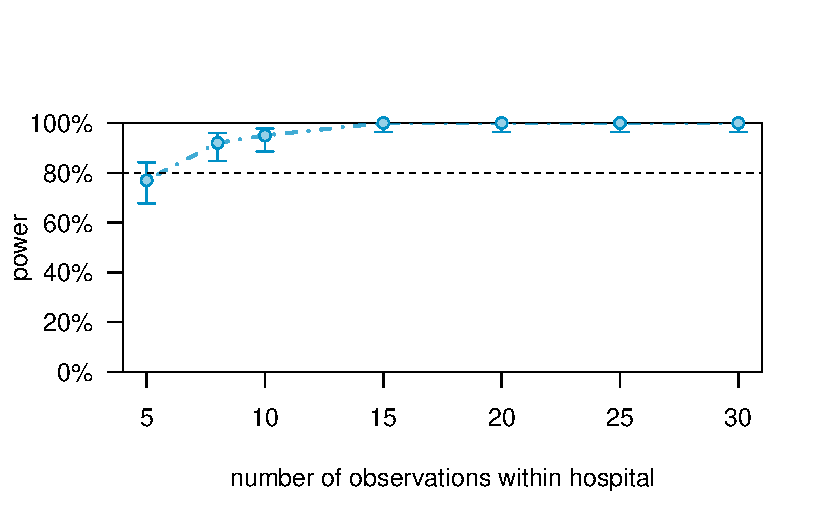
\includegraphics[width=0.9\textwidth,height=\textheight]{05a-experimental-design_files/figure-pdf/fig-simr-power-curve-1.pdf}

}

\caption{\label{fig-simr-power-curve}Simulation-based power curve for
the cardiac rehabilitation mixed model, varying the number of patients
per hospital. The dashed red line marks 80\% power. With a treatment
effect of 5 recovery points, hospital-level SD of 3, and residual SD of
8, approximately 8 patients per hospital are needed to achieve 80\%
power when 10 hospitals are available. Shaded bands show 95\% confidence
intervals around the power estimates based on 100 simulations.}

\end{figure}%

\begin{Shaded}
\begin{Highlighting}[]
\CommentTok{\# Extend along hospitals: vary number of hospitals}
\NormalTok{fit\_extended\_along }\OtherTok{\textless{}{-}} \FunctionTok{extend}\NormalTok{(}
\NormalTok{  fit\_pilot,}
  \AttributeTok{along =} \StringTok{"hospital"}\NormalTok{,}
  \AttributeTok{n =} \DecValTok{20}
\NormalTok{)}

\CommentTok{\# Power curve across number of hospitals}
\NormalTok{power\_curve\_hospitals }\OtherTok{\textless{}{-}} \FunctionTok{powerCurve}\NormalTok{(}
\NormalTok{  fit\_extended\_along,}
  \AttributeTok{test   =} \FunctionTok{fixed}\NormalTok{(}\StringTok{"treatmentTreatment"}\NormalTok{, }\AttributeTok{method =} \StringTok{"t"}\NormalTok{),}
  \AttributeTok{along  =} \StringTok{"hospital"}\NormalTok{,}
  \AttributeTok{breaks =} \FunctionTok{c}\NormalTok{(}\DecValTok{5}\NormalTok{, }\DecValTok{6}\NormalTok{, }\DecValTok{8}\NormalTok{, }\DecValTok{10}\NormalTok{, }\DecValTok{15}\NormalTok{, }\DecValTok{20}\NormalTok{),}
  \AttributeTok{nsim   =} \DecValTok{100}
\NormalTok{)}
\end{Highlighting}
\end{Shaded}

\begin{verbatim}
#> Calculating power at 6 sample sizes along hospital
\end{verbatim}

\begin{verbatim}
#> Simulating: |                                                                  |Simulating: |=                                                                 |Simulating: |==                                                                |Simulating: |===                                                               |Simulating: |====                                                              |Simulating: |=====                                                             |Simulating: |======                                                            |Simulating: |=======                                                           |Simulating: |========                                                          |Simulating: |=========                                                         |Simulating: |==========                                                        |Simulating: |===========                                                       |Simulating: |============                                                      |Simulating: |=============                                                     |Simulating: |==============                                                    |Simulating: |===============                                                   |Simulating: |================                                                  |Simulating: |=================                                                 |Simulating: |==================                                                |Simulating: |===================                                               |Simulating: |====================                                              |Simulating: |=====================                                             |Simulating: |======================                                            |Simulating: |=======================                                           |Simulating: |========================                                          |Simulating: |=========================                                         |Simulating: |==========================                                        |Simulating: |===========================                                       |Simulating: |============================                                      |Simulating: |=============================                                     |Simulating: |==============================                                    |Simulating: |===============================                                   |Simulating: |================================                                  |Simulating: |=================================                                 |Simulating: |==================================                                |Simulating: |===================================                               |Simulating: |====================================                              |Simulating: |=====================================                             |Simulating: |======================================                            |Simulating: |=======================================                           |Simulating: |========================================                          |Simulating: |=========================================                         |Simulating: |==========================================                        |Simulating: |===========================================                       |Simulating: |============================================                      |Simulating: |=============================================                     |Simulating: |==============================================                    |Simulating: |===============================================                   |Simulating: |================================================                  |Simulating: |=================================================                 |Simulating: |==================================================                |Simulating: |===================================================               |Simulating: |====================================================              |Simulating: |=====================================================             |Simulating: |======================================================            |Simulating: |=======================================================           |Simulating: |========================================================          |Simulating: |=========================================================         |Simulating: |==========================================================        |Simulating: |===========================================================       |Simulating: |============================================================      |Simulating: |=============================================================     |Simulating: |==============================================================    |Simulating: |===============================================================   |Simulating: |================================================================  |Simulating: |================================================================= |Simulating: |==================================================================|(1/6) (1/6) Simulating: |                                                            |(1/6) Simulating: |=                                                           |(1/6) Simulating: |==                                                          |(1/6) Simulating: |===                                                         |(1/6) Simulating: |====                                                        |(1/6) Simulating: |=====                                                       |(1/6) Simulating: |======                                                      |(1/6) Simulating: |=======                                                     |(1/6) Simulating: |========                                                    |(1/6) Simulating: |=========                                                   |(1/6) Simulating: |==========                                                  |(1/6) Simulating: |===========                                                 |(1/6) Simulating: |============                                                |(1/6) Simulating: |=============                                               |(1/6) Simulating: |==============                                              |(1/6) Simulating: |===============                                             |(1/6) Simulating: |================                                            |(1/6) Simulating: |=================                                           |(1/6) Simulating: |==================                                          |(1/6) Simulating: |===================                                         |(1/6) Simulating: |====================                                        |(1/6) Simulating: |=====================                                       |(1/6) Simulating: |======================                                      |(1/6) Simulating: |=======================                                     |(1/6) Simulating: |========================                                    |(1/6) Simulating: |=========================                                   |(1/6) Simulating: |==========================                                  |(1/6) Simulating: |===========================                                 |(1/6) Simulating: |============================                                |(1/6) Simulating: |=============================                               |(1/6) Simulating: |==============================                              |(1/6) Simulating: |===============================                             |(1/6) Simulating: |================================                            |(1/6) Simulating: |=================================                           |(1/6) Simulating: |==================================                          |(1/6) Simulating: |===================================                         |(1/6) Simulating: |====================================                        |(1/6) Simulating: |=====================================                       |(1/6) Simulating: |======================================                      |(1/6) Simulating: |=======================================                     |(1/6) Simulating: |========================================                    |(1/6) Simulating: |=========================================                   |(1/6) Simulating: |==========================================                  |(1/6) Simulating: |===========================================                 |(1/6) Simulating: |============================================                |(1/6) Simulating: |=============================================               |(1/6) Simulating: |==============================================              |(1/6) Simulating: |===============================================             |(1/6) Simulating: |================================================            |(1/6) Simulating: |=================================================           |(1/6) Simulating: |==================================================          |(1/6) Simulating: |===================================================         |(1/6) Simulating: |====================================================        |(1/6) Simulating: |=====================================================       |(1/6) Simulating: |======================================================      |(1/6) Simulating: |=======================================================     |(1/6) Simulating: |========================================================    |(1/6) Simulating: |=========================================================   |(1/6) Simulating: |==========================================================  |(1/6) Simulating: |=========================================================== |(1/6) Simulating: |============================================================|(1/6) (2/6) (2/6) Simulating: |                                                            |(2/6) Simulating: |=                                                           |(2/6) Simulating: |==                                                          |(2/6) Simulating: |===                                                         |(2/6) Simulating: |====                                                        |(2/6) Simulating: |=====                                                       |(2/6) Simulating: |======                                                      |(2/6) Simulating: |=======                                                     |(2/6) Simulating: |========                                                    |(2/6) Simulating: |=========                                                   |(2/6) Simulating: |==========                                                  |(2/6) Simulating: |===========                                                 |(2/6) Simulating: |============                                                |(2/6) Simulating: |=============                                               |(2/6) Simulating: |==============                                              |(2/6) Simulating: |===============                                             |(2/6) Simulating: |================                                            |(2/6) Simulating: |=================                                           |(2/6) Simulating: |==================                                          |(2/6) Simulating: |===================                                         |(2/6) Simulating: |====================                                        |(2/6) Simulating: |=====================                                       |(2/6) Simulating: |======================                                      |(2/6) Simulating: |=======================                                     |(2/6) Simulating: |========================                                    |(2/6) Simulating: |=========================                                   |(2/6) Simulating: |==========================                                  |(2/6) Simulating: |===========================                                 |(2/6) Simulating: |============================                                |(2/6) Simulating: |=============================                               |(2/6) Simulating: |==============================                              |(2/6) Simulating: |===============================                             |(2/6) Simulating: |================================                            |(2/6) Simulating: |=================================                           |(2/6) Simulating: |==================================                          |(2/6) Simulating: |===================================                         |(2/6) Simulating: |====================================                        |(2/6) Simulating: |=====================================                       |(2/6) Simulating: |======================================                      |(2/6) Simulating: |=======================================                     |(2/6) Simulating: |========================================                    |(2/6) Simulating: |=========================================                   |(2/6) Simulating: |==========================================                  |(2/6) Simulating: |===========================================                 |(2/6) Simulating: |============================================                |(2/6) Simulating: |=============================================               |(2/6) Simulating: |==============================================              |(2/6) Simulating: |===============================================             |(2/6) Simulating: |================================================            |(2/6) Simulating: |=================================================           |(2/6) Simulating: |==================================================          |(2/6) Simulating: |===================================================         |(2/6) Simulating: |====================================================        |(2/6) Simulating: |=====================================================       |(2/6) Simulating: |======================================================      |(2/6) Simulating: |=======================================================     |(2/6) Simulating: |========================================================    |(2/6) Simulating: |=========================================================   |(2/6) Simulating: |==========================================================  |(2/6) Simulating: |=========================================================== |(2/6) Simulating: |============================================================|(2/6) (3/6) (3/6) Simulating: |                                                            |(3/6) Simulating: |=                                                           |(3/6) Simulating: |==                                                          |(3/6) Simulating: |===                                                         |(3/6) Simulating: |====                                                        |(3/6) Simulating: |=====                                                       |(3/6) Simulating: |======                                                      |(3/6) Simulating: |=======                                                     |(3/6) Simulating: |========                                                    |(3/6) Simulating: |=========                                                   |(3/6) Simulating: |==========                                                  |(3/6) Simulating: |===========                                                 |(3/6) Simulating: |============                                                |(3/6) Simulating: |=============                                               |(3/6) Simulating: |==============                                              |(3/6) Simulating: |===============                                             |(3/6) Simulating: |================                                            |(3/6) Simulating: |=================                                           |(3/6) Simulating: |==================                                          |(3/6) Simulating: |===================                                         |(3/6) Simulating: |====================                                        |(3/6) Simulating: |=====================                                       |(3/6) Simulating: |======================                                      |(3/6) Simulating: |=======================                                     |(3/6) Simulating: |========================                                    |(3/6) Simulating: |=========================                                   |(3/6) Simulating: |==========================                                  |(3/6) Simulating: |===========================                                 |(3/6) Simulating: |============================                                |(3/6) Simulating: |=============================                               |(3/6) Simulating: |==============================                              |(3/6) Simulating: |===============================                             |(3/6) Simulating: |================================                            |(3/6) Simulating: |=================================                           |(3/6) Simulating: |==================================                          |(3/6) Simulating: |===================================                         |(3/6) Simulating: |====================================                        |(3/6) Simulating: |=====================================                       |(3/6) Simulating: |======================================                      |(3/6) Simulating: |=======================================                     |(3/6) Simulating: |========================================                    |(3/6) Simulating: |=========================================                   |(3/6) Simulating: |==========================================                  |(3/6) Simulating: |===========================================                 |(3/6) Simulating: |============================================                |(3/6) Simulating: |=============================================               |(3/6) Simulating: |==============================================              |(3/6) Simulating: |===============================================             |(3/6) Simulating: |================================================            |(3/6) Simulating: |=================================================           |(3/6) Simulating: |==================================================          |(3/6) Simulating: |===================================================         |(3/6) Simulating: |====================================================        |(3/6) Simulating: |=====================================================       |(3/6) Simulating: |======================================================      |(3/6) Simulating: |=======================================================     |(3/6) Simulating: |========================================================    |(3/6) Simulating: |=========================================================   |(3/6) Simulating: |==========================================================  |(3/6) Simulating: |=========================================================== |(3/6) Simulating: |============================================================|(3/6) (4/6) (4/6) Simulating: |                                                            |(4/6) Simulating: |=                                                           |(4/6) Simulating: |==                                                          |(4/6) Simulating: |===                                                         |(4/6) Simulating: |====                                                        |(4/6) Simulating: |=====                                                       |(4/6) Simulating: |======                                                      |(4/6) Simulating: |=======                                                     |(4/6) Simulating: |========                                                    |(4/6) Simulating: |=========                                                   |(4/6) Simulating: |==========                                                  |(4/6) Simulating: |===========                                                 |(4/6) Simulating: |============                                                |(4/6) Simulating: |=============                                               |(4/6) Simulating: |==============                                              |(4/6) Simulating: |===============                                             |(4/6) Simulating: |================                                            |(4/6) Simulating: |=================                                           |(4/6) Simulating: |==================                                          |(4/6) Simulating: |===================                                         |(4/6) Simulating: |====================                                        |(4/6) Simulating: |=====================                                       |(4/6) Simulating: |======================                                      |(4/6) Simulating: |=======================                                     |(4/6) Simulating: |========================                                    |(4/6) Simulating: |=========================                                   |(4/6) Simulating: |==========================                                  |(4/6) Simulating: |===========================                                 |(4/6) Simulating: |============================                                |(4/6) Simulating: |=============================                               |(4/6) Simulating: |==============================                              |(4/6) Simulating: |===============================                             |(4/6) Simulating: |================================                            |(4/6) Simulating: |=================================                           |(4/6) Simulating: |==================================                          |(4/6) Simulating: |===================================                         |(4/6) Simulating: |====================================                        |(4/6) Simulating: |=====================================                       |(4/6) Simulating: |======================================                      |(4/6) Simulating: |=======================================                     |(4/6) Simulating: |========================================                    |(4/6) Simulating: |=========================================                   |(4/6) Simulating: |==========================================                  |(4/6) Simulating: |===========================================                 |(4/6) Simulating: |============================================                |(4/6) Simulating: |=============================================               |(4/6) Simulating: |==============================================              |(4/6) Simulating: |===============================================             |(4/6) Simulating: |================================================            |(4/6) Simulating: |=================================================           |(4/6) Simulating: |==================================================          |(4/6) Simulating: |===================================================         |(4/6) Simulating: |====================================================        |(4/6) Simulating: |=====================================================       |(4/6) Simulating: |======================================================      |(4/6) Simulating: |=======================================================     |(4/6) Simulating: |========================================================    |(4/6) Simulating: |=========================================================   |(4/6) Simulating: |==========================================================  |(4/6) Simulating: |=========================================================== |(4/6) Simulating: |============================================================|(4/6) (5/6) (5/6) Simulating: |                                                            |(5/6) Simulating: |=                                                           |(5/6) Simulating: |==                                                          |(5/6) Simulating: |===                                                         |(5/6) Simulating: |====                                                        |(5/6) Simulating: |=====                                                       |(5/6) Simulating: |======                                                      |(5/6) Simulating: |=======                                                     |(5/6) Simulating: |========                                                    |(5/6) Simulating: |=========                                                   |(5/6) Simulating: |==========                                                  |(5/6) Simulating: |===========                                                 |(5/6) Simulating: |============                                                |(5/6) Simulating: |=============                                               |(5/6) Simulating: |==============                                              |(5/6) Simulating: |===============                                             |(5/6) Simulating: |================                                            |(5/6) Simulating: |=================                                           |(5/6) Simulating: |==================                                          |(5/6) Simulating: |===================                                         |(5/6) Simulating: |====================                                        |(5/6) Simulating: |=====================                                       |(5/6) Simulating: |======================                                      |(5/6) Simulating: |=======================                                     |(5/6) Simulating: |========================                                    |(5/6) Simulating: |=========================                                   |(5/6) Simulating: |==========================                                  |(5/6) Simulating: |===========================                                 |(5/6) Simulating: |============================                                |(5/6) Simulating: |=============================                               |(5/6) Simulating: |==============================                              |(5/6) Simulating: |===============================                             |(5/6) Simulating: |================================                            |(5/6) Simulating: |=================================                           |(5/6) Simulating: |==================================                          |(5/6) Simulating: |===================================                         |(5/6) Simulating: |====================================                        |(5/6) Simulating: |=====================================                       |(5/6) Simulating: |======================================                      |(5/6) Simulating: |=======================================                     |(5/6) Simulating: |========================================                    |(5/6) Simulating: |=========================================                   |(5/6) Simulating: |==========================================                  |(5/6) Simulating: |===========================================                 |(5/6) Simulating: |============================================                |(5/6) Simulating: |=============================================               |(5/6) Simulating: |==============================================              |(5/6) Simulating: |===============================================             |(5/6) Simulating: |================================================            |(5/6) Simulating: |=================================================           |(5/6) Simulating: |==================================================          |(5/6) Simulating: |===================================================         |(5/6) Simulating: |====================================================        |(5/6) Simulating: |=====================================================       |(5/6) Simulating: |======================================================      |(5/6) Simulating: |=======================================================     |(5/6) Simulating: |========================================================    |(5/6) Simulating: |=========================================================   |(5/6) Simulating: |==========================================================  |(5/6) Simulating: |=========================================================== |(5/6) Simulating: |============================================================|(5/6) (6/6) (6/6) Simulating: |                                                            |(6/6) Simulating: |=                                                           |(6/6) Simulating: |==                                                          |(6/6) Simulating: |===                                                         |(6/6) Simulating: |====                                                        |(6/6) Simulating: |=====                                                       |(6/6) Simulating: |======                                                      |(6/6) Simulating: |=======                                                     |(6/6) Simulating: |========                                                    |(6/6) Simulating: |=========                                                   |(6/6) Simulating: |==========                                                  |(6/6) Simulating: |===========                                                 |(6/6) Simulating: |============                                                |(6/6) Simulating: |=============                                               |(6/6) Simulating: |==============                                              |(6/6) Simulating: |===============                                             |(6/6) Simulating: |================                                            |(6/6) Simulating: |=================                                           |(6/6) Simulating: |==================                                          |(6/6) Simulating: |===================                                         |(6/6) Simulating: |====================                                        |(6/6) Simulating: |=====================                                       |(6/6) Simulating: |======================                                      |(6/6) Simulating: |=======================                                     |(6/6) Simulating: |========================                                    |(6/6) Simulating: |=========================                                   |(6/6) Simulating: |==========================                                  |(6/6) Simulating: |===========================                                 |(6/6) Simulating: |============================                                |(6/6) Simulating: |=============================                               |(6/6) Simulating: |==============================                              |(6/6) Simulating: |===============================                             |(6/6) Simulating: |================================                            |(6/6) Simulating: |=================================                           |(6/6) Simulating: |==================================                          |(6/6) Simulating: |===================================                         |(6/6) Simulating: |====================================                        |(6/6) Simulating: |=====================================                       |(6/6) Simulating: |======================================                      |(6/6) Simulating: |=======================================                     |(6/6) Simulating: |========================================                    |(6/6) Simulating: |=========================================                   |(6/6) Simulating: |==========================================                  |(6/6) Simulating: |===========================================                 |(6/6) Simulating: |============================================                |(6/6) Simulating: |=============================================               |(6/6) Simulating: |==============================================              |(6/6) Simulating: |===============================================             |(6/6) Simulating: |================================================            |(6/6) Simulating: |=================================================           |(6/6) Simulating: |==================================================          |(6/6) Simulating: |===================================================         |(6/6) Simulating: |====================================================        |(6/6) Simulating: |=====================================================       |(6/6) Simulating: |======================================================      |(6/6) Simulating: |=======================================================     |(6/6) Simulating: |========================================================    |(6/6) Simulating: |=========================================================   |(6/6) Simulating: |==========================================================  |(6/6) Simulating: |=========================================================== |(6/6) Simulating: |============================================================|(6/6) 
\end{verbatim}

\begin{Shaded}
\begin{Highlighting}[]
\FunctionTok{print}\NormalTok{(power\_curve\_hospitals)}
\end{Highlighting}
\end{Shaded}

\begin{verbatim}
#> Power for predictor 'treatmentTreatment', (95% confidence interval),
#> by number of levels in hospital:
#>       5: 59.00% (48.71, 68.74) - 52 rows
#>       6: 66.00% (55.85, 75.18) - 60 rows
#>       8: 79.00% (69.71, 86.51) - 81 rows
#>      10: 87.00% (78.80, 92.89) - 97 rows
#>      15: 96.00% (90.07, 98.90) - 148 rows
#>      20: 99.00% (94.55, 99.97) - 200 rows
#> 
#> (0 errors, 0 warnings, 6 messages)
#> 
#> Time elapsed: 0 h 0 m 51 s
\end{verbatim}

\begin{Shaded}
\begin{Highlighting}[]
\FunctionTok{plot}\NormalTok{(power\_curve\_hospitals)}
\end{Highlighting}
\end{Shaded}

\begin{figure}[H]

\centering{

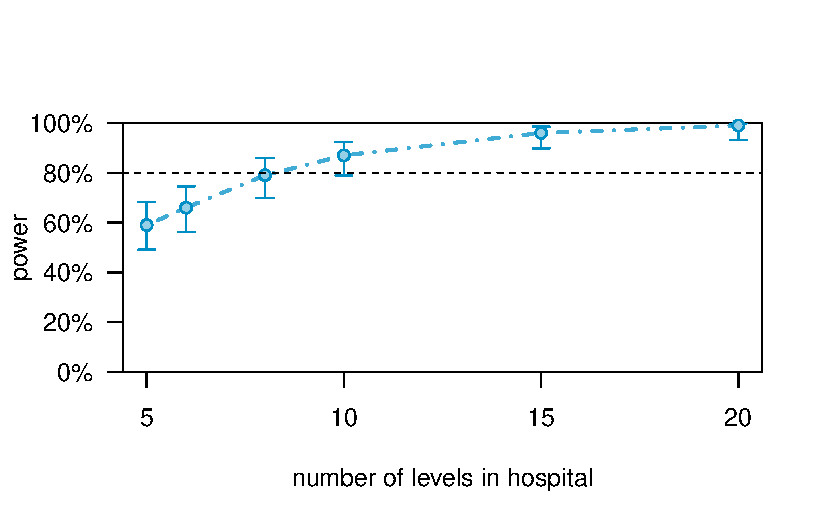
\includegraphics[width=0.9\textwidth,height=\textheight]{05a-experimental-design_files/figure-pdf/fig-simr-power-hospitals-1.pdf}

}

\caption{\label{fig-simr-power-hospitals}Simulation-based power curve
for the cardiac rehabilitation mixed model, varying the number of
hospitals. The dashed red line marks 80\% power. Approximately 8-10
hospitals are needed to achieve 80\% power with 10 patients per hospital
and a treatment effect of 5 recovery points. Shaded bands show 95\%
confidence intervals around the power estimates based on 100
simulations.}

\end{figure}%

\subsection{Reading the Output}\label{reading-the-output}

The two power curves tell a clear and instructive story about how
replication at different levels of the hierarchy contributes to power.

\textbf{Varying the number of hospitals} (the higher-level unit): power
climbs from 59\% with 5 hospitals to 79\% with 8 hospitals, crossing the
80\% threshold between 8 and 10 hospitals. At 10 hospitals the power
reaches 87\% (95\% CI: \([79, 93]\)), and at 15 hospitals it is 96\%. To
achieve 80\% power for a treatment effect of 5 recovery points with 10
patients per hospital, the study needs approximately \textbf{8-10
hospitals}.

\textbf{Varying the number of patients per hospital} (the lower-level
unit): power is already 77\% at 5 patients per hospital and reaches 92\%
at 8 patients, crossing the 80\% threshold between 5 and 8 patients. At
10 patients per hospital it reaches 95\%, and at 15 patients it is
essentially 100\%.

At first glance, adding patients per hospital appears more efficient
than adding hospitals, 8 patients per hospital gives 92\% power, while 8
hospitals with 10 patients each gives only 79\%. But this comparison is
misleading, because the two curves are asking different questions with
different total sample sizes. At 8 hospitals with 10 patients each, the
total sample is 80 patients. At 10 hospitals with 8 patients each, the
total is also 80 patients. The within-hospital curve reaches higher
power at the same total \(N\) because adding patients within hospitals
reduces the residual variance more efficiently when the hospital-level
variance is already accounted for as a random effect.

The deeper point is that \textbf{both dimensions of replication matter,
but for different reasons.} The number of hospitals determines the
degrees of freedom for the treatment test, treatment is tested against
between-hospital variation, and more hospitals means more information
about that variation. The number of patients per hospital determines the
precision of each hospital's mean estimate. For this particular variance
structure (hospital SD = 3, residual SD = 8), the residual variation is
larger than the hospital-level variation, so adding patients within
hospitals is the more efficient investment per additional observation.
In a study where hospital-level variation dominated, the opposite would
be true.

\subsection{\texorpdfstring{A Note on \texttt{method\ =\ "t"} vs
\texttt{method\ =\ "kr"} in
\texttt{powerSim}}{A Note on method = "t" vs method = "kr" in powerSim}}\label{a-note-on-method-t-vs-method-kr-in-powersim}

Students familiar with Chapter \ref{sec-chap9} will notice that we used
\texttt{method\ =\ "t"} (Satterthwaite approximation) in the
\texttt{powerSim} call rather than \texttt{method\ =\ "kr"}
(Kenward-Roger), which was recommended for small numbers of groups in
Chapter \ref{sec-chap9}. The reason is practical rather than principled.

\texttt{simr} works by repeatedly simulating new response data from the
fitted model, refitting the model to each simulated dataset, and
extracting a test result. The Kenward-Roger method via \texttt{pbkrtest}
involves a more complex internal model comparison that can conflict with
the way \texttt{simr} handles model refitting, specifically, it attempts
to drop terms from the model in a way that fails when \texttt{simr} has
modified the model structure for simulation purposes. This produces the
``scope is not a subset of term labels'' error.

The Satterthwaite method (\texttt{method\ =\ "t"}) works directly on the
summary output of the refitted model and does not attempt any internal
model comparison, making it compatible with \texttt{simr}'s simulation
loop.

For power analysis purposes, the difference between Satterthwaite and
Kenward-Roger is small and does not materially affect the sample size
recommendation. Both methods give conservative tests relative to the
naive z-test, and for the sample sizes relevant to power analysis, where
you are asking whether a study is large enough, the distinction is
negligible. The Kenward-Roger correction matters most when reporting the
final analysis of a completed study with a small number of groups; at
that stage, use \texttt{anova(fit,\ ddf\ =\ "Kenward-Roger")} as
recommended in Chapter \ref{sec-chap9}. For the prospective power
calculation, Satterthwaite is an entirely acceptable and stable choice.

\subsection{The Key Advantage Over Analytical Power
Formulas}\label{the-key-advantage-over-analytical-power-formulas}

The \texttt{simr} approach has three advantages that matter for complex
designs.

\textbf{It respects the actual model structure.} The power calculation
uses the estimated variance components, the hospital-level variance and
the residual variance, from the fitted model directly, rather than
requiring you to specify them separately as inputs to a formula. If your
pilot data suggest that hospital-level variation is large, the power
estimate will reflect this automatically.

\textbf{It can test any effect in any model.} \texttt{powerSim()} works
for any fixed effect in any model that \texttt{lme4} can fit, crossed
random effects, random slopes, interaction terms, and GLMMs via
\texttt{glmer}. There is no analytical formula for the power of an
interaction term in a three-level nested GLMM; \texttt{simr} handles it
without modification.

\textbf{It separates two design decisions.} \texttt{extend()} can vary
the number of higher-level units (hospitals) or the number of
lower-level units (patients per hospital) independently, allowing you to
ask which dimension of replication is more valuable for a given budget.
In hierarchical designs, adding higher-level units (more hospitals)
almost always increases power more efficiently than adding lower-level
units (more patients per hospital), because the treatment is tested
against between-hospital variation, not between-patient variation.
\texttt{powerCurve()} with both \texttt{along} and \texttt{within} makes
this trade-off visible.

\subsection{\texorpdfstring{Practical Recommendations for Using
\texttt{simr}}{Practical Recommendations for Using simr}}\label{practical-recommendations-for-using-simr}

Use \texttt{nsim\ =\ 100} during exploration to find the approximate
sample size quickly, then rerun with \texttt{nsim\ =\ 500} or
\texttt{nsim\ =\ 1000} for the final estimate reported in a grant
application or pre-registration. The confidence interval on the power
estimate narrows as \(1/\sqrt{n_{\text{sim}}}\), so quadrupling the
simulations halves the uncertainty.

Always check that the model used for power analysis matches the model
you intend to fit, the same random effects structure, the same link
function for GLMMs, and the same degrees of freedom method. A power
analysis conducted for a Satterthwaite model but reported as a
Kenward-Roger analysis will give slightly different results.

\subsection{Reporting the Power
Analysis}\label{reporting-the-power-analysis}

Power analyses should be reported in the Methods section of a paper,
before the Results, under a dedicated subsection. The report must
contain enough information for a reader to verify the calculation and
assess whether the study was adequately powered. Here is a template
based on the results above:

\begin{quote}
\textbf{Sample size and power.} Sample size was determined using
simulation-based power analysis conducted with the \texttt{simr} package
version x.x.x \citep{Green2016} in R version x.x.x (R Core Team, 2026).
The intended analysis was a linear mixed-effects model with treatment
(control vs intervention) as a fixed effect and a random intercept for
hospital, fitted using \texttt{lme4} \citep{Bates2015}. Power was
estimated for a minimum clinically meaningful treatment effect of 5
recovery points, based on a between-hospital standard deviation of 3
points and a residual standard deviation of 8 points derived from a
preliminary survey of the literature. The Satterthwaite t-test was used
for all power simulations. Power was estimated across a range of sample
sizes using 100 simulations per design point; final estimates were
confirmed with 500 simulations.

Power analysis indicated that 10 hospitals with 10 patients per hospital
(total \(N = 100\)) would provide 87\% power (95\% simulation CI:
\([79, 93]\)\%) to detect a treatment effect of 5 recovery points at
\(\alpha = 0.05\). To allow for an anticipated dropout rate of 10\%, we
planned to recruit 12 patients per hospital, giving a target total of
\(N = 120\) patients across 10 hospitals.
\end{quote}

\subsection{What Must Be Included}\label{what-must-be-included}

Every power analysis report must contain the following elements. Missing
any of them makes the analysis unverifiable:

\begin{longtable}[]{@{}
  >{\raggedright\arraybackslash}p{(\columnwidth - 2\tabcolsep) * \real{0.5000}}
  >{\raggedright\arraybackslash}p{(\columnwidth - 2\tabcolsep) * \real{0.5000}}@{}}
\toprule\noalign{}
\begin{minipage}[b]{\linewidth}\raggedright
Element
\end{minipage} & \begin{minipage}[b]{\linewidth}\raggedright
Example
\end{minipage} \\
\midrule\noalign{}
\endhead
\bottomrule\noalign{}
\endlastfoot
Software and version & \texttt{simr} version 1.0.7, R 4.4.0 \\
Intended statistical model & Linear mixed model with random intercept
for hospital \\
Effect size and its justification & 5 recovery points; minimum
clinically meaningful difference \\
Variance components & Between-hospital SD = 3, residual SD = 8 \\
Significance threshold & \(\alpha = 0.05\) \\
Target power & 80\% (or 90\% for clinical confirmatory trials) \\
Number of simulations & 100 exploratory, 500 confirmatory \\
Final sample size chosen & 10 hospitals \(\times\) 12 patients = 120 \\
Attrition adjustment & 10\% over-recruitment \\
\end{longtable}

\subsection{A Common Mistake: Reporting Post Hoc
Power}\label{a-common-mistake-reporting-post-hoc-power}

A frequent error in published papers is to report power \emph{after} the
analysis, computing the power the study had to detect the observed
effect. This is called \textbf{post hoc power} or \textbf{observed
power}, and it is uninformative. When a result is significant, the post
hoc power will always be high; when it is non-significant, the post hoc
power will always be low. The calculation adds nothing to what the
p-value already tells you and should not be reported.

If a study yields a non-significant result and you want to assess
whether a meaningful effect might have been missed, the correct tool is
a \textbf{confidence interval around the effect size}, not a post hoc
power calculation. A wide confidence interval that includes both zero
and a clinically meaningful effect tells you directly that the study was
underpowered for the question of interest, and it does so honestly,
without the circular logic of post hoc power.

\subsection{Specifying the Effect Size
Honestly}\label{specifying-the-effect-size-honestly}

The hardest part of power analysis is specifying the effect size. Three
approaches are available, in order of preference:

\textbf{From prior literature.} Previous studies with the same response
variable and similar treatments provide effect size estimates. Apply
conservatism, published effect sizes are inflated by publication bias.
Use the lower bound of a confidence interval around the published effect
rather than the point estimate.

\textbf{From a pilot study.} A small preliminary experiment provides an
estimate of the within-group variance (the denominator of the effect
size) grounded in your specific biological system. With fewer than 10
units per group, the variance estimate will be imprecise, but it is more
honest than a guess.

\textbf{From the minimum biologically meaningful effect.} Ask: what is
the smallest difference that would be scientifically or practically
important? A drug that reduces tumour size by 1mm may be statistically
detectable but clinically irrelevant. Power the study to detect the
smallest effect that would change a decision or conclusion, not the
smallest effect that exists.

Using Cohen's conventional benchmarks (small = 0.2, medium = 0.5, large
= 0.8 for Cohen's d) as a substitute for genuine subject matter
knowledge is the least defensible approach. Conventions calibrated on
social psychology experiments from the 1960s have no particular
relevance to the effect sizes typical in your biological system.

\subsection{The Multiple Testing Problem in
Design}\label{the-multiple-testing-problem-in-design}

If your experiment involves multiple primary outcomes or multiple
pairwise comparisons, the power analysis must account for the multiple
testing correction that will be applied at the analysis stage. Adjusting
p-values downward (via Bonferroni, Holm, or Tukey) reduces the effective
alpha for each test and therefore reduces power. The sample size
calculation must use the corrected alpha, not the nominal 0.05.

\begin{Shaded}
\begin{Highlighting}[]
\FunctionTok{library}\NormalTok{(pwr)}

\CommentTok{\# Power for one{-}way ANOVA with 4 groups (6 pairwise comparisons)}
\CommentTok{\# Using Bonferroni{-}corrected alpha for pairwise tests}
\NormalTok{alpha\_corrected }\OtherTok{\textless{}{-}} \FloatTok{0.05} \SpecialCharTok{/} \FunctionTok{choose}\NormalTok{(}\DecValTok{4}\NormalTok{, }\DecValTok{2}\NormalTok{)   }\CommentTok{\# 0.05 / 6}

\FunctionTok{cat}\NormalTok{(}\StringTok{"Bonferroni{-}corrected alpha:"}\NormalTok{, }\FunctionTok{round}\NormalTok{(alpha\_corrected, }\DecValTok{4}\NormalTok{), }\StringTok{"}\SpecialCharTok{\textbackslash{}n}\StringTok{"}\NormalTok{)}
\end{Highlighting}
\end{Shaded}

\begin{verbatim}
#> Bonferroni-corrected alpha: 0.0083
\end{verbatim}

\begin{Shaded}
\begin{Highlighting}[]
\CommentTok{\# Sample size needed per group with correction}
\FunctionTok{pwr.t.test}\NormalTok{(}\AttributeTok{d         =} \FloatTok{0.5}\NormalTok{,}
           \AttributeTok{sig.level =}\NormalTok{ alpha\_corrected,}
           \AttributeTok{power     =} \FloatTok{0.80}\NormalTok{,}
           \AttributeTok{type      =} \StringTok{"two.sample"}\NormalTok{)}
\end{Highlighting}
\end{Shaded}

\begin{verbatim}
#> 
#>      Two-sample t test power calculation 
#> 
#>               n = 98.62942
#>               d = 0.5
#>       sig.level = 0.008333333
#>           power = 0.8
#>     alternative = two.sided
#> 
#> NOTE: n is number in *each* group
\end{verbatim}

The corrected alpha requires substantially larger samples than the
nominal 0.05 would suggest, a direct consequence of the multiple testing
overhead that is easy to overlook at the design stage and costly to
discover at the analysis stage.

\subsection{A Design Checklist}\label{a-design-checklist}

Before finalising any experimental design, work through the following
questions:

\textbf{Randomisation:}

\begin{itemize}
\item
  Is every experimental unit randomly assigned to a treatment?
\item
  Is the randomisation documented and reproducible?
\item
  Are any known confounders balanced across treatment groups?
\end{itemize}

\textbf{Replication:}

\begin{itemize}
\item
  What is the experimental unit i.e.~the entity that received the
  treatment independently?
\item
  How many independent replicates are there per treatment at the level
  of the experimental unit?
\item
  Is this number justified by a power analysis?
\end{itemize}

\textbf{Blocking:} - Are there known sources of nuisance variation?

\begin{itemize}
\item
  Can they be controlled by blocking before randomisation?
\item
  Is the block factor included in the intended analysis?
\end{itemize}

\textbf{Analysis:} - Is the intended model formula written down?

\begin{itemize}
\item
  Does it match the design, specifically the randomisation structure and
  the hierarchy of units?
\item
  Has the power been calculated for the primary comparison using the
  intended analysis?
\end{itemize}

\textbf{Practical:} - Is the expected attrition rate accounted for in
the sample size?

\begin{itemize}
\item
  Is the response variable sensitive and precise enough to detect the
  effect of interest?
\item
  Are all measurements taken blind to treatment allocation where
  possible?
\end{itemize}

A design that passes all of these checks will not guarantee a
significant result, nothing can do that, but it will guarantee that
whatever result emerges is worth trusting.

\begin{tcolorbox}[enhanced jigsaw, title=\textcolor{quarto-callout-note-color}{\faInfo}\hspace{0.5em}{Going Further}, opacityback=0, bottomtitle=1mm, leftrule=.75mm, breakable, toprule=.15mm, colframe=quarto-callout-note-color-frame, titlerule=0mm, rightrule=.15mm, toptitle=1mm, arc=.35mm, colback=white, left=2mm, colbacktitle=quarto-callout-note-color!10!white, opacitybacktitle=0.6, coltitle=black, bottomrule=.15mm]

\begin{itemize}
\item
  \textbf{Cox, D. R., \& Reid, N. (2000). The Theory of the Design of
  Experiments. CRC Press.} The theoretical foundation for readers who
  want to understand randomisation theory, optimality criteria, and the
  mathematical basis for why blocking works. Not light reading, but
  authoritative.
\item
  \textbf{Quinn, G. P., \& Keough, M. J. (2002). Experimental Design and
  Data Analysis for Biologists. Cambridge University Press.} A
  comprehensive experimental design reference specifically written for
  biologists. Covers randomisation, blocking, factorial designs, and
  split-plot in much greater depth.
\item
  \textbf{Mead, R., Gilmour, S. G., \& Mead, A. (2012). Statistical
  Principles for the Design of Experiments. Cambridge University Press.}
  Specifically focused on the principles rather than the computations.
  It adress why designs work, what makes a good design, how to choose
  among alternatives.
\item
  \textbf{Lawson, J. (2014). Design and Analysis of Experiments with R.
  CRC Press.} The most directly R-oriented design textbook available.
  Every design in this book. A natural companion for students.
\item
  \textbf{Montgomery, D. C. (2017). Design and Analysis of Experiments
  (9th ed.). Wiley.} The engineering-oriented classic that covers every
  design mentioned in this book and many more. The book is Heavier on
  mathematics than Quinn \& Keough but authoritative and thorough.
\end{itemize}

\end{tcolorbox}

\chapter{Reporting ANOVA Results}\label{sec-chap13}

Running a correct analysis is necessary but not sufficient. The analysis
must also be reported in a way that allows readers to evaluate the
evidence, reproduce the findings, and build on the work. Poorly reported
statistics are a persistent problem in the biological literature, not
always because the analysis was wrong, but because essential information
was omitted, the visualisation was misleading, or the narrative obscured
rather than illuminated the findings.

This chapter covers what must appear in a paper, how to visualise
results honestly and effectively, and provides templates for the Methods
and Results sections that can be adapted for any ANOVA design covered in
this book.

\section{What Must Appear in a Paper}\label{what-must-appear-in-a-paper}

\subsection{The Minimum Reporting
Standard}\label{the-minimum-reporting-standard}

Every reported ANOVA result should contain, at minimum, the following
information:

\textbf{The test statistic and its degrees of freedom.} For an \(F\)
test: \(F_{df_1, df_2} = x.xx\). Both degrees of freedom are required,
the numerator (\(df_1\)) and the denominator (\(df_2\)). A reported
\(F\) without degrees of freedom cannot be verified or reproduced.

\textbf{The p-value.} Report exact p-values to two or three significant
figures (e.g.~\(p = 0.023\), \(p = 0.003\)), not as inequalities unless
the value is below a reporting threshold (e.g.~\(p < 0.001\)). The
convention of reporting \(p < 0.05\) as ``significant'' and \(p > 0.05\)
as ``not significant'' without the actual value discards information
that readers need to form their own judgements.

\textbf{An effect size with a confidence interval.} As Chapter
\ref{sec-chap3} demonstrated, the p-value conflates the size of the
effect with the size of the study. Always accompany the \(F\) test with
\(\eta^2\), \(\omega^2\), or partial \(\omega^2\) as appropriate, with a
95\% confidence interval. For pairwise comparisons, report the estimated
difference (or ratio for log-link models) and its confidence interval.

\textbf{The sample size.} Total \(N\) and the number of observations per
group. For nested or hierarchical designs, report the sample size at
every relevant level, the number of subjects, the number of observations
per subject, and the number of groups.

\textbf{The software and packages used.} Specify R version and the
version of every package used in the analysis. Results from
\texttt{lme4}, \texttt{glmmTMB}, \texttt{emmeans}, and
\texttt{effectsize} can differ across versions.

\subsection{Reporting Mixed Models}\label{reporting-mixed-models}

Mixed models require additional reporting beyond standard ANOVA:

\begin{itemize}
\tightlist
\item
  The full model formula, ideally in R notation.
\item
  The estimation method (REML or ML) and the rationale.
\item
  The method used for degrees of freedom and p-values (Satterthwaite or
  Kenward-Roger).
\item
  The variance components (\(\hat{\sigma}^2_b\) and
  \(\hat{\sigma}^2_\varepsilon\)) and the ICC.
\item
  The conditional and marginal \(R^2\) values.
\end{itemize}

\subsection{Reporting GLMMs}\label{reporting-glmms}

For GLMMs, report additionally:

\begin{itemize}
\tightlist
\item
  The response distribution and link function.
\item
  Evidence that the model was adequately specified (DHARMa diagnostics,
  overdispersion ratio).
\item
  Coefficients on both the link scale (for statistical inference) and
  the response scale (for biological interpretation), e.g.~log-odds
  ratios and odds ratios for binomial models, log-rate ratios and rate
  ratios for Poisson models.
\item
  For zero-inflated models, report the zero-inflation component
  separately from the conditional component.
\end{itemize}

\subsection{Common Reporting Mistakes}\label{common-reporting-mistakes}

The following are frequently seen in published papers and should be
avoided:

\begin{longtable}[]{@{}
  >{\raggedright\arraybackslash}p{(\columnwidth - 2\tabcolsep) * \real{0.3462}}
  >{\raggedright\arraybackslash}p{(\columnwidth - 2\tabcolsep) * \real{0.6538}}@{}}
\toprule\noalign{}
\begin{minipage}[b]{\linewidth}\raggedright
Mistake
\end{minipage} & \begin{minipage}[b]{\linewidth}\raggedright
Correct practice
\end{minipage} \\
\midrule\noalign{}
\endhead
\bottomrule\noalign{}
\endlastfoot
Reporting only \(p < 0.05\) & Report exact \(p\)-value \\
Omitting degrees of freedom & Always report \(F_{df_1, df_2}\) \\
No effect size & Report \(\omega^2\) or partial \(\omega^2\) \\
``Mean ± SE'' without stating what SE means & State standard error of
the mean explicitly \\
No post-hoc method specified & Name the correction (Tukey, Holm,
etc.) \\
No software version & Cite R version and package versions \\
No model formula for mixed models & Include full \texttt{lmer()}
formula \\
Reporting ANOVA without assumption checks & Report key diagnostics \\
\end{longtable}

\section{Visualisation}\label{visualisation}

Good visualisation shows the data, not just the summary. The most common
visualisation mistake in biology is replacing individual observations
with bars and error bars, a format that hides the distribution of the
data and makes it impossible to assess assumptions visually. The
sections below progress from least to most informative.

\subsection{Means Plots}\label{means-plots}

Means plots display the group mean with an error bar representing either
the standard error or the 95\% confidence interval. They are familiar
and compact but convey almost no information about the distribution of
the data.

\begin{Shaded}
\begin{Highlighting}[]
\FunctionTok{library}\NormalTok{(ggplot2)}

\FunctionTok{set.seed}\NormalTok{(}\DecValTok{42}\NormalTok{)}
\NormalTok{n     }\OtherTok{\textless{}{-}} \DecValTok{20}
\NormalTok{group }\OtherTok{\textless{}{-}} \FunctionTok{factor}\NormalTok{(}\FunctionTok{rep}\NormalTok{(}\FunctionTok{c}\NormalTok{(}\StringTok{"Control"}\NormalTok{, }\StringTok{"Nitrogen"}\NormalTok{, }\StringTok{"Phosphorus"}\NormalTok{),}
                    \AttributeTok{each =}\NormalTok{ n),}
                \AttributeTok{levels =} \FunctionTok{c}\NormalTok{(}\StringTok{"Control"}\NormalTok{, }\StringTok{"Nitrogen"}\NormalTok{, }\StringTok{"Phosphorus"}\NormalTok{))}
\NormalTok{y     }\OtherTok{\textless{}{-}} \FunctionTok{c}\NormalTok{(}\FunctionTok{rnorm}\NormalTok{(n, }\DecValTok{20}\NormalTok{, }\DecValTok{3}\NormalTok{), }\FunctionTok{rnorm}\NormalTok{(n, }\DecValTok{25}\NormalTok{, }\DecValTok{3}\NormalTok{), }\FunctionTok{rnorm}\NormalTok{(n, }\DecValTok{22}\NormalTok{, }\DecValTok{3}\NormalTok{))}
\NormalTok{df    }\OtherTok{\textless{}{-}} \FunctionTok{data.frame}\NormalTok{(y, group)}

\CommentTok{\# Compute means and CIs}
\NormalTok{summ }\OtherTok{\textless{}{-}} \FunctionTok{do.call}\NormalTok{(rbind, }\FunctionTok{lapply}\NormalTok{(}\FunctionTok{levels}\NormalTok{(group), }\ControlFlowTok{function}\NormalTok{(g) \{}
\NormalTok{  x   }\OtherTok{\textless{}{-}}\NormalTok{ df}\SpecialCharTok{$}\NormalTok{y[df}\SpecialCharTok{$}\NormalTok{group }\SpecialCharTok{==}\NormalTok{ g]}
\NormalTok{  m   }\OtherTok{\textless{}{-}} \FunctionTok{mean}\NormalTok{(x)}
\NormalTok{  se  }\OtherTok{\textless{}{-}} \FunctionTok{sd}\NormalTok{(x) }\SpecialCharTok{/} \FunctionTok{sqrt}\NormalTok{(}\FunctionTok{length}\NormalTok{(x))}
\NormalTok{  ci  }\OtherTok{\textless{}{-}} \FunctionTok{qt}\NormalTok{(}\FloatTok{0.975}\NormalTok{, }\AttributeTok{df =} \FunctionTok{length}\NormalTok{(x) }\SpecialCharTok{{-}} \DecValTok{1}\NormalTok{) }\SpecialCharTok{*}\NormalTok{ se}
  \FunctionTok{data.frame}\NormalTok{(}\AttributeTok{group =}\NormalTok{ g, }\AttributeTok{mean =}\NormalTok{ m, }\AttributeTok{lower =}\NormalTok{ m }\SpecialCharTok{{-}}\NormalTok{ ci, }\AttributeTok{upper =}\NormalTok{ m }\SpecialCharTok{+}\NormalTok{ ci)}
\NormalTok{\}))}
\NormalTok{summ}\SpecialCharTok{$}\NormalTok{group }\OtherTok{\textless{}{-}} \FunctionTok{factor}\NormalTok{(summ}\SpecialCharTok{$}\NormalTok{group, }\AttributeTok{levels =} \FunctionTok{levels}\NormalTok{(group))}

\FunctionTok{ggplot}\NormalTok{(summ, }\FunctionTok{aes}\NormalTok{(}\AttributeTok{x =}\NormalTok{ group, }\AttributeTok{y =}\NormalTok{ mean, }\AttributeTok{colour =}\NormalTok{ group)) }\SpecialCharTok{+}
  \FunctionTok{geom\_pointrange}\NormalTok{(}\FunctionTok{aes}\NormalTok{(}\AttributeTok{ymin =}\NormalTok{ lower, }\AttributeTok{ymax =}\NormalTok{ upper),}
                  \AttributeTok{size =} \DecValTok{1}\NormalTok{, }\AttributeTok{linewidth =} \FloatTok{1.2}\NormalTok{) }\SpecialCharTok{+}
  \FunctionTok{scale\_colour\_manual}\NormalTok{(}\AttributeTok{values =} \FunctionTok{c}\NormalTok{(}\StringTok{"\#2E86AB"}\NormalTok{, }\StringTok{"\#F6AE2D"}\NormalTok{,}
                                 \StringTok{"\#E84855"}\NormalTok{)) }\SpecialCharTok{+}
  \FunctionTok{labs}\NormalTok{(}\AttributeTok{title    =} \StringTok{"Means plot with 95\% confidence intervals"}\NormalTok{,}
       \AttributeTok{subtitle =} \StringTok{"Error bars show 95\% CI"}\NormalTok{,}
       \AttributeTok{x =} \ConstantTok{NULL}\NormalTok{, }\AttributeTok{y =} \StringTok{"Plant height (cm)"}\NormalTok{) }\SpecialCharTok{+}
  \FunctionTok{theme\_bw}\NormalTok{() }\SpecialCharTok{+}
  \FunctionTok{theme}\NormalTok{(}\AttributeTok{legend.position =} \StringTok{"none"}\NormalTok{)}
\end{Highlighting}
\end{Shaded}

\begin{figure}[H]

\centering{

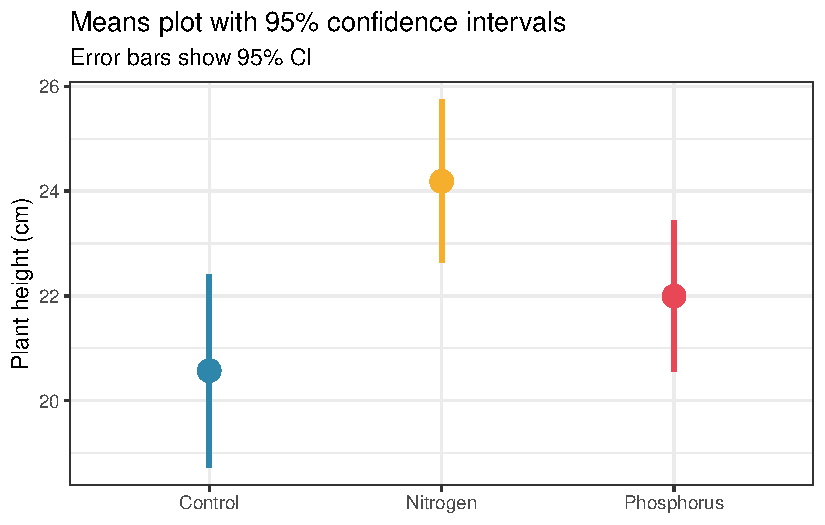
\includegraphics[width=0.9\textwidth,height=\textheight]{05b-reporting_files/figure-pdf/fig-means-plot-1.pdf}

}

\caption{\label{fig-means-plot}Means plot with 95\% confidence intervals
for the fertiliser experiment. While compact and familiar, this format
hides the distribution of the data, two datasets with identical means
and CIs can have completely different distributions. Use with caution
and always accompany with a more informative display.}

\end{figure}%

If you use a means plot, always:

\begin{itemize}
\tightlist
\item
  State explicitly what the error bars represent (SE, SD, or CI).
\item
  Use 95\% CIs rather than SE: CIs are directly interpretable for
  inference, SE bars are not.
\item
  Accompany with the sample size per group in the figure caption.
\end{itemize}

\subsection{Boxplots}\label{boxplots}

Boxplots display the median, interquartile range, and outliers. They
convey more information than a means plot and are appropriate for
moderate sample sizes (\(n \geq 10\) per group). For small samples they
can be misleading, a boxplot of five points looks authoritative but
represents very little data.

\begin{Shaded}
\begin{Highlighting}[]
\FunctionTok{ggplot}\NormalTok{(df, }\FunctionTok{aes}\NormalTok{(}\AttributeTok{x =}\NormalTok{ group, }\AttributeTok{y =}\NormalTok{ y, }\AttributeTok{fill =}\NormalTok{ group)) }\SpecialCharTok{+}
  \FunctionTok{geom\_boxplot}\NormalTok{(}\AttributeTok{alpha   =} \FloatTok{0.4}\NormalTok{,}
               \AttributeTok{outlier.shape =} \ConstantTok{NA}\NormalTok{,}
               \AttributeTok{width   =} \FloatTok{0.5}\NormalTok{) }\SpecialCharTok{+}
  \FunctionTok{geom\_jitter}\NormalTok{(}\AttributeTok{width =} \FloatTok{0.1}\NormalTok{, }\AttributeTok{size =} \DecValTok{2}\NormalTok{, }\AttributeTok{alpha =} \FloatTok{0.6}\NormalTok{,}
              \FunctionTok{aes}\NormalTok{(}\AttributeTok{colour =}\NormalTok{ group)) }\SpecialCharTok{+}
  \FunctionTok{scale\_fill\_manual}\NormalTok{(}\AttributeTok{values   =} \FunctionTok{c}\NormalTok{(}\StringTok{"\#2E86AB"}\NormalTok{, }\StringTok{"\#F6AE2D"}\NormalTok{,}
                                 \StringTok{"\#E84855"}\NormalTok{)) }\SpecialCharTok{+}
  \FunctionTok{scale\_colour\_manual}\NormalTok{(}\AttributeTok{values =} \FunctionTok{c}\NormalTok{(}\StringTok{"\#2E86AB"}\NormalTok{, }\StringTok{"\#F6AE2D"}\NormalTok{,}
                                 \StringTok{"\#E84855"}\NormalTok{)) }\SpecialCharTok{+}
  \FunctionTok{labs}\NormalTok{(}\AttributeTok{title    =} \StringTok{"Boxplot with individual observations"}\NormalTok{,}
       \AttributeTok{subtitle =} \FunctionTok{paste0}\NormalTok{(}\StringTok{"n = "}\NormalTok{, n, }\StringTok{" per group"}\NormalTok{),}
       \AttributeTok{x =} \ConstantTok{NULL}\NormalTok{, }\AttributeTok{y =} \StringTok{"Plant height (cm)"}\NormalTok{) }\SpecialCharTok{+}
  \FunctionTok{theme\_bw}\NormalTok{() }\SpecialCharTok{+}
  \FunctionTok{theme}\NormalTok{(}\AttributeTok{legend.position =} \StringTok{"none"}\NormalTok{)}
\end{Highlighting}
\end{Shaded}

\begin{figure}[H]

\centering{

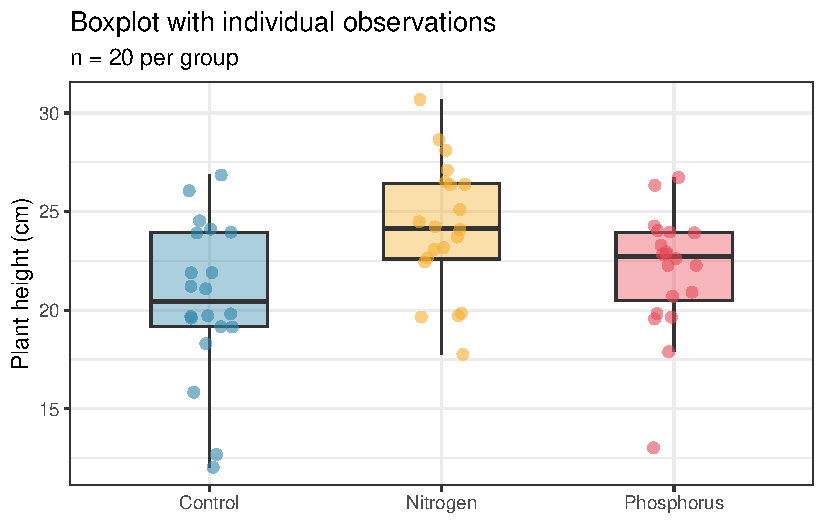
\includegraphics[width=0.9\textwidth,height=\textheight]{05b-reporting_files/figure-pdf/fig-boxplot-1.pdf}

}

\caption{\label{fig-boxplot}Boxplot with individual observations
overlaid for the fertiliser experiment. The boxplot shows the median,
interquartile range, and outliers; the jittered points show every
individual observation. This combination is the minimum acceptable
display for biological data.}

\end{figure}%

Always overlay the individual data points when \(n < 50\) per group. The
\texttt{outlier.shape\ =\ NA} argument removes the duplicate outlier
points that \texttt{geom\_boxplot} would otherwise add, since all points
are shown by \texttt{geom\_jitter}, the boxplot outliers become
redundant and confusing.

\subsection{Violin Plots}\label{violin-plots}

Violin plots show the full distribution as a kernel density estimate,
mirrored to form a symmetric shape. They are more informative than
boxplots for large samples (\(n > 30\) per group) where the shape of the
distribution matters.

\begin{Shaded}
\begin{Highlighting}[]
\FunctionTok{ggplot}\NormalTok{(df, }\FunctionTok{aes}\NormalTok{(}\AttributeTok{x =}\NormalTok{ group, }\AttributeTok{y =}\NormalTok{ y, }\AttributeTok{fill =}\NormalTok{ group)) }\SpecialCharTok{+}
  \FunctionTok{geom\_violin}\NormalTok{(}\AttributeTok{alpha =} \FloatTok{0.4}\NormalTok{, }\AttributeTok{trim =} \ConstantTok{FALSE}\NormalTok{) }\SpecialCharTok{+}
  \FunctionTok{geom\_boxplot}\NormalTok{(}\AttributeTok{width   =} \FloatTok{0.1}\NormalTok{,}
               \AttributeTok{fill    =} \StringTok{"white"}\NormalTok{,}
               \AttributeTok{outlier.shape =} \ConstantTok{NA}\NormalTok{,}
               \AttributeTok{alpha   =} \FloatTok{0.8}\NormalTok{) }\SpecialCharTok{+}
  \FunctionTok{geom\_jitter}\NormalTok{(}\AttributeTok{width =} \FloatTok{0.05}\NormalTok{, }\AttributeTok{size =} \FloatTok{1.5}\NormalTok{, }\AttributeTok{alpha =} \FloatTok{0.5}\NormalTok{,}
              \FunctionTok{aes}\NormalTok{(}\AttributeTok{colour =}\NormalTok{ group)) }\SpecialCharTok{+}
  \FunctionTok{scale\_fill\_manual}\NormalTok{(}\AttributeTok{values   =} \FunctionTok{c}\NormalTok{(}\StringTok{"\#2E86AB"}\NormalTok{, }\StringTok{"\#F6AE2D"}\NormalTok{,}
                                 \StringTok{"\#E84855"}\NormalTok{)) }\SpecialCharTok{+}
  \FunctionTok{scale\_colour\_manual}\NormalTok{(}\AttributeTok{values =} \FunctionTok{c}\NormalTok{(}\StringTok{"\#2E86AB"}\NormalTok{, }\StringTok{"\#F6AE2D"}\NormalTok{,}
                                 \StringTok{"\#E84855"}\NormalTok{)) }\SpecialCharTok{+}
  \FunctionTok{labs}\NormalTok{(}\AttributeTok{title    =} \StringTok{"Violin plot with embedded boxplot"}\NormalTok{,}
       \AttributeTok{subtitle =} \FunctionTok{paste0}\NormalTok{(}\StringTok{"n = "}\NormalTok{, n, }\StringTok{" per group"}\NormalTok{),}
       \AttributeTok{x =} \ConstantTok{NULL}\NormalTok{, }\AttributeTok{y =} \StringTok{"Plant height (cm)"}\NormalTok{) }\SpecialCharTok{+}
  \FunctionTok{theme\_bw}\NormalTok{() }\SpecialCharTok{+}
  \FunctionTok{theme}\NormalTok{(}\AttributeTok{legend.position =} \StringTok{"none"}\NormalTok{)}
\end{Highlighting}
\end{Shaded}

\begin{figure}[H]

\centering{

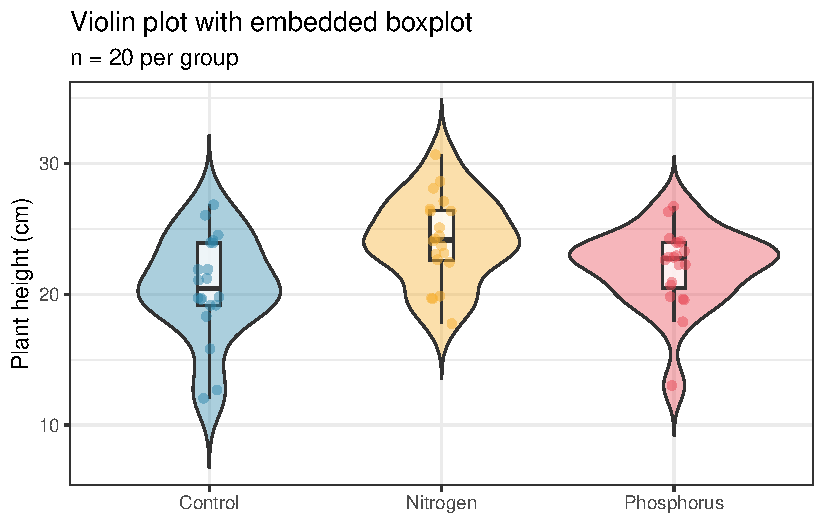
\includegraphics[width=0.9\textwidth,height=\textheight]{05b-reporting_files/figure-pdf/fig-violin-plot-1.pdf}

}

\caption{\label{fig-violin-plot}Violin plot with embedded boxplot and
individual observations for the fertiliser experiment. The violin shape
shows the full distribution; the inner boxplot provides the summary
statistics; the points show individual observations. This is the most
complete single-panel display for group comparisons.}

\end{figure}%

\subsection{Adding Significance
Annotations}\label{adding-significance-annotations}

Post-hoc comparison results can be added directly to the plot using the
\texttt{ggpubr} or \texttt{ggsignif} packages:

\begin{Shaded}
\begin{Highlighting}[]
\CommentTok{\# install.packages("ggsignif") if needed}
\FunctionTok{library}\NormalTok{(ggsignif)}

\CommentTok{\# Run Tukey HSD first}
\NormalTok{fit   }\OtherTok{\textless{}{-}} \FunctionTok{aov}\NormalTok{(y }\SpecialCharTok{\textasciitilde{}}\NormalTok{ group, }\AttributeTok{data =}\NormalTok{ df)}
\NormalTok{tukey }\OtherTok{\textless{}{-}} \FunctionTok{TukeyHSD}\NormalTok{(fit)}
\FunctionTok{print}\NormalTok{(tukey)}
\end{Highlighting}
\end{Shaded}

\begin{verbatim}
#>   Tukey multiple comparisons of means
#>     95% family-wise confidence level
#> 
#> Fit: aov(formula = y ~ group, data = df)
#> 
#> $group
#>                          diff       lwr       upr     p adj
#> Nitrogen-Control     3.611265  0.974554 6.2479751 0.0047467
#> Phosphorus-Control   1.421508 -1.215203 4.0582183 0.4025112
#> Phosphorus-Nitrogen -2.189757 -4.826467 0.4469538 0.1218054
\end{verbatim}

\begin{Shaded}
\begin{Highlighting}[]
\FunctionTok{ggplot}\NormalTok{(df, }\FunctionTok{aes}\NormalTok{(}\AttributeTok{x =}\NormalTok{ group, }\AttributeTok{y =}\NormalTok{ y, }\AttributeTok{fill =}\NormalTok{ group)) }\SpecialCharTok{+}
  \FunctionTok{geom\_boxplot}\NormalTok{(}\AttributeTok{alpha   =} \FloatTok{0.4}\NormalTok{,}
               \AttributeTok{outlier.shape =} \ConstantTok{NA}\NormalTok{,}
               \AttributeTok{width   =} \FloatTok{0.5}\NormalTok{) }\SpecialCharTok{+}
  \FunctionTok{geom\_jitter}\NormalTok{(}\AttributeTok{width =} \FloatTok{0.1}\NormalTok{, }\AttributeTok{size =} \DecValTok{2}\NormalTok{, }\AttributeTok{alpha =} \FloatTok{0.6}\NormalTok{,}
              \FunctionTok{aes}\NormalTok{(}\AttributeTok{colour =}\NormalTok{ group)) }\SpecialCharTok{+}
  \FunctionTok{geom\_signif}\NormalTok{(}
    \AttributeTok{comparisons     =} \FunctionTok{list}\NormalTok{(}\FunctionTok{c}\NormalTok{(}\StringTok{"Control"}\NormalTok{, }\StringTok{"Nitrogen"}\NormalTok{),}
                           \FunctionTok{c}\NormalTok{(}\StringTok{"Control"}\NormalTok{, }\StringTok{"Phosphorus"}\NormalTok{)),}
    \AttributeTok{map\_signif\_level =} \ConstantTok{TRUE}\NormalTok{,}
    \AttributeTok{tip\_length      =} \FloatTok{0.02}\NormalTok{,}
    \AttributeTok{y\_position      =} \FunctionTok{c}\NormalTok{(}\DecValTok{29}\NormalTok{, }\DecValTok{31}\NormalTok{)}
\NormalTok{  ) }\SpecialCharTok{+}
  \FunctionTok{scale\_fill\_manual}\NormalTok{(}\AttributeTok{values   =} \FunctionTok{c}\NormalTok{(}\StringTok{"\#2E86AB"}\NormalTok{, }\StringTok{"\#F6AE2D"}\NormalTok{,}
                                 \StringTok{"\#E84855"}\NormalTok{)) }\SpecialCharTok{+}
  \FunctionTok{scale\_colour\_manual}\NormalTok{(}\AttributeTok{values =} \FunctionTok{c}\NormalTok{(}\StringTok{"\#2E86AB"}\NormalTok{, }\StringTok{"\#F6AE2D"}\NormalTok{,}
                                 \StringTok{"\#E84855"}\NormalTok{)) }\SpecialCharTok{+}
  \FunctionTok{labs}\NormalTok{(}\AttributeTok{title    =} \StringTok{"Post{-}hoc comparisons on a boxplot"}\NormalTok{,}
       \AttributeTok{subtitle =} \StringTok{"Tukey HSD; * p \textless{} 0.05, ** p \textless{} 0.01, *** p \textless{} 0.001"}\NormalTok{,}
       \AttributeTok{x =} \ConstantTok{NULL}\NormalTok{, }\AttributeTok{y =} \StringTok{"Plant height (cm)"}\NormalTok{) }\SpecialCharTok{+}
  \FunctionTok{theme\_bw}\NormalTok{() }\SpecialCharTok{+}
  \FunctionTok{theme}\NormalTok{(}\AttributeTok{legend.position =} \StringTok{"none"}\NormalTok{)}
\end{Highlighting}
\end{Shaded}

\begin{figure}[H]

\centering{

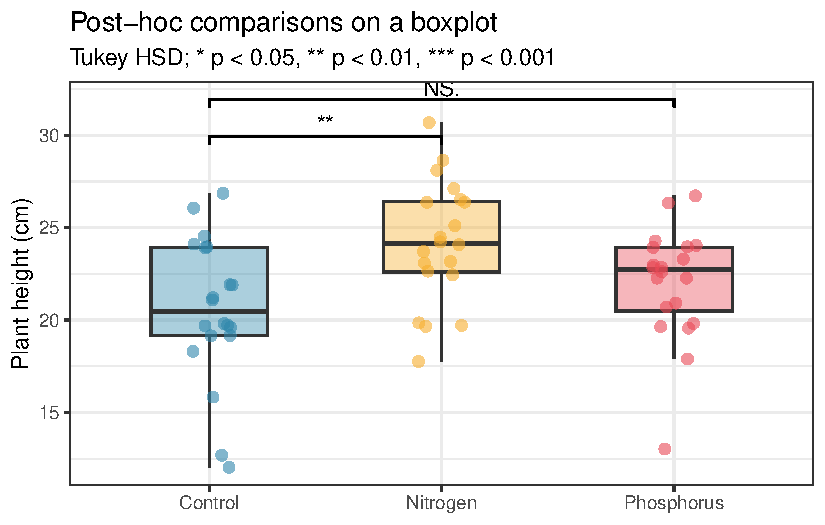
\includegraphics[width=0.9\textwidth,height=\textheight]{05b-reporting_files/figure-pdf/fig-significance-annotation-1.pdf}

}

\caption{\label{fig-significance-annotation}Boxplot with Tukey HSD
significance annotations. Only significant comparisons are annotated;
non-significant pairs are left unannotated. The annotation style follows
the convention of placing brackets between compared groups with the
adjusted p-value or significance stars.}

\end{figure}%

\subsection{Forest Plots for Multi-Study or Multi-Comparison
Results}\label{forest-plots-for-multi-study-or-multi-comparison-results}

Forest plots display point estimates and confidence intervals for
multiple comparisons or studies simultaneously, making it easy to
compare effect sizes and their uncertainty across a set of results. They
are standard in meta-analysis but are equally valuable for displaying a
set of post-hoc comparisons or the results of multiple related ANOVA
models.

\begin{Shaded}
\begin{Highlighting}[]
\FunctionTok{library}\NormalTok{(ggplot2)}

\CommentTok{\# Extract Tukey HSD results into a data frame}
\NormalTok{tukey\_df }\OtherTok{\textless{}{-}} \FunctionTok{as.data.frame}\NormalTok{(tukey}\SpecialCharTok{$}\NormalTok{group)}
\NormalTok{tukey\_df}\SpecialCharTok{$}\NormalTok{comparison }\OtherTok{\textless{}{-}} \FunctionTok{rownames}\NormalTok{(tukey\_df)}
\FunctionTok{names}\NormalTok{(tukey\_df)[}\DecValTok{1}\SpecialCharTok{:}\DecValTok{4}\NormalTok{] }\OtherTok{\textless{}{-}} \FunctionTok{c}\NormalTok{(}\StringTok{"estimate"}\NormalTok{, }\StringTok{"lower"}\NormalTok{, }\StringTok{"upper"}\NormalTok{, }\StringTok{"p\_adj"}\NormalTok{)}

\NormalTok{tukey\_df}\SpecialCharTok{$}\NormalTok{significant }\OtherTok{\textless{}{-}} \FunctionTok{ifelse}\NormalTok{(tukey\_df}\SpecialCharTok{$}\NormalTok{p\_adj }\SpecialCharTok{\textless{}} \FloatTok{0.05}\NormalTok{,}
                                \StringTok{"Significant"}\NormalTok{, }\StringTok{"Non{-}significant"}\NormalTok{)}
\NormalTok{tukey\_df}\SpecialCharTok{$}\NormalTok{comparison }\OtherTok{\textless{}{-}} \FunctionTok{factor}\NormalTok{(tukey\_df}\SpecialCharTok{$}\NormalTok{comparison,}
                               \AttributeTok{levels =} \FunctionTok{rev}\NormalTok{(tukey\_df}\SpecialCharTok{$}\NormalTok{comparison))}

\FunctionTok{ggplot}\NormalTok{(tukey\_df,}
       \FunctionTok{aes}\NormalTok{(}\AttributeTok{x =}\NormalTok{ estimate, }\AttributeTok{y =}\NormalTok{ comparison,}
           \AttributeTok{xmin =}\NormalTok{ lower, }\AttributeTok{xmax =}\NormalTok{ upper,}
           \AttributeTok{colour =}\NormalTok{ significant)) }\SpecialCharTok{+}
  \FunctionTok{geom\_vline}\NormalTok{(}\AttributeTok{xintercept =} \DecValTok{0}\NormalTok{,}
             \AttributeTok{linetype =} \StringTok{"dashed"}\NormalTok{, }\AttributeTok{colour =} \StringTok{"grey50"}\NormalTok{,}
             \AttributeTok{linewidth =} \FloatTok{0.8}\NormalTok{) }\SpecialCharTok{+}
  \FunctionTok{geom\_errorbarh}\NormalTok{(}\AttributeTok{height =} \FloatTok{0.2}\NormalTok{, }\AttributeTok{linewidth =} \DecValTok{1}\NormalTok{) }\SpecialCharTok{+}
  \FunctionTok{geom\_point}\NormalTok{(}\AttributeTok{size =} \DecValTok{4}\NormalTok{) }\SpecialCharTok{+}
  \FunctionTok{scale\_colour\_manual}\NormalTok{(}\AttributeTok{values =} \FunctionTok{c}\NormalTok{(}\StringTok{"Significant"}     \OtherTok{=} \StringTok{"\#E84855"}\NormalTok{,}
                                 \StringTok{"Non{-}significant"} \OtherTok{=} \StringTok{"\#2E86AB"}\NormalTok{)) }\SpecialCharTok{+}
  \FunctionTok{labs}\NormalTok{(}
    \AttributeTok{title    =} \StringTok{"Tukey HSD pairwise comparisons"}\NormalTok{,}
    \AttributeTok{subtitle =} \StringTok{"Points = estimated mean difference; lines = 95\% CI"}\NormalTok{,}
    \AttributeTok{x        =} \StringTok{"Mean difference in plant height (cm)"}\NormalTok{,}
    \AttributeTok{y        =} \ConstantTok{NULL}\NormalTok{,}
    \AttributeTok{colour   =} \ConstantTok{NULL}
\NormalTok{  ) }\SpecialCharTok{+}
  \FunctionTok{theme\_bw}\NormalTok{() }\SpecialCharTok{+}
  \FunctionTok{theme}\NormalTok{(}\AttributeTok{legend.position =} \StringTok{"bottom"}\NormalTok{)}
\end{Highlighting}
\end{Shaded}

\begin{verbatim}
#> Warning: `geom_errorbarh()` was deprecated in ggplot2 4.0.0.
#> i Please use the `orientation` argument of `geom_errorbar()` instead.
\end{verbatim}

\begin{verbatim}
#> `height` was translated to `width`.
\end{verbatim}

\begin{figure}[H]

\centering{

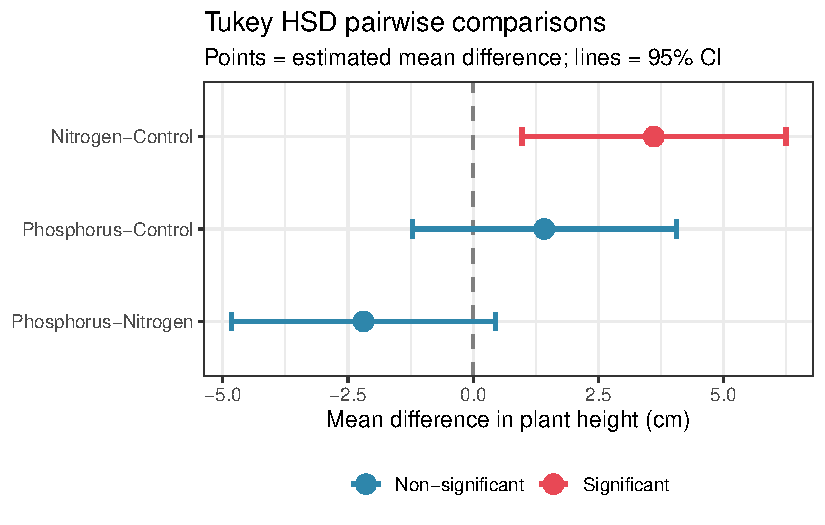
\includegraphics[width=0.9\textwidth,height=\textheight]{05b-reporting_files/figure-pdf/fig-forest-plot-1.pdf}

}

\caption{\label{fig-forest-plot}Forest plot of Tukey HSD pairwise
comparisons from the fertiliser experiment. Each row is one comparison;
points show the estimated mean difference; horizontal lines show the
95\% CI. The vertical dashed line at zero marks no difference,
comparisons whose CI does not cross zero are significant after Tukey
correction.}

\end{figure}%

Forest plots become particularly valuable when you have many comparisons
to display, for example, the results of a two-way ANOVA with post-hoc
comparisons within each level of one factor, or the treatment effects
from the same model fitted to multiple response variables. They are
superior to tables for communicating patterns across many estimates
because the eye can immediately detect which estimates are large, which
are imprecise, and which are consistent in direction.

\subsection{Choosing the Right
Visualisation}\label{choosing-the-right-visualisation}

\begin{longtable}[]{@{}ll@{}}
\toprule\noalign{}
Situation & Recommended plot \\
\midrule\noalign{}
\endhead
\bottomrule\noalign{}
\endlastfoot
\(n < 10\) per group & Dot plot with all points shown \\
\(10 \leq n < 30\) & Boxplot with jittered points \\
\(n \geq 30\) & Violin plot with embedded boxplot \\
Many groups (\(k > 6\)) & Horizontal boxplot or dot plot \\
Longitudinal data & Line plot with individual trajectories \\
Post-hoc comparisons & Forest plot \\
Interaction effects & Interaction plot with CIs \\
Effect sizes across studies & Forest plot \\
\end{longtable}

\begin{center}\rule{0.5\linewidth}{0.5pt}\end{center}

\section{A Template for Methods and Results
Sections}\label{a-template-for-methods-and-results-sections}

\subsection{One-Way ANOVA}\label{one-way-anova}

\textbf{Methods:}

\begin{quote}
The effect of fertiliser type (control, nitrogen, phosphorus) on plant
height was analysed using one-way ANOVA. Residual normality was assessed
using a Q-Q plot and the Shapiro-Wilk test; homogeneity of variance was
assessed using Levene's test. Pairwise comparisons between groups were
conducted using Tukey's HSD test. Effect size was quantified using
omega-squared (\(\omega^2\)) with 95\% confidence intervals computed
using the \texttt{effectsize} package \citep{Ben-Shachar2020}. All
analyses were conducted in R version x.x.x \citep{R2024} using the
\texttt{car} \citep{Fox2019} and \texttt{effectsize} packages.
\end{quote}

\textbf{Results:}

\begin{quote}
Fertiliser type had a significant effect on plant height
(\(F_{2,57} = x.xx\), \(p = x.xxx\), \(\omega^2 = x.xx\), 95\% CI:
\([x.xx, x.xx]\)). Post-hoc Tukey HSD comparisons revealed that
nitrogen-treated plants were significantly taller than control plants
(mean difference = \(x.x\) cm, 95\% CI: \([x.x, x.x]\), \(p = x.xxx\))
and phosphorus-treated plants (mean difference = \(x.x\) cm, 95\% CI:
\([x.x, x.x]\), \(p = x.xxx\)). Phosphorus-treated and control plants
did not differ significantly (mean difference = \(x.x\) cm, 95\% CI:
\([x.x, x.x]\), \(p = x.xxx\)). Group means (± SD) were \(x.x
\pm x.x\) cm (control), \(x.x \pm x.x\) cm (nitrogen), and
\(x.x \pm x.x\) cm (phosphorus).
\end{quote}

\subsection{Two-Way ANOVA}\label{two-way-anova}

\textbf{Methods:}

\begin{quote}
The effects of fertiliser type (control, nitrogen, phosphorus) and
watering regime (dry, watered) on plant yield were analysed using a
two-way ANOVA with Type III sums of squares (using sum-to-zero
contrasts), fitted with the \texttt{lm()} function in R and tested using
\texttt{car::Anova()} \citep{Fox2011}. Residual diagnostics were
conducted as above. The interaction was examined first; where
significant, simple main effects were tested within each level of the
other factor using \texttt{emmeans} \citep{Lenth2026} with Tukey
adjustment.
\end{quote}

\textbf{Results:}

\begin{quote}
A significant fertiliser \(\times\) watering interaction was found
(\(F_{2,54} = x.xx\), \(p = x.xxx\), partial \(\omega^2
= x.xx\)). Simple effects analysis revealed that the effect of
fertiliser differed between dry and watered conditions {[}describe the
specific pattern{]}. Main effects of fertiliser (\(F_{2,54} = x.xx\),
\(p = x.xxx\)) and watering (\(F_{1,54} = x.xx\), \(p = x.xxx\)) are not
interpreted independently given the significant interaction.
\end{quote}

\subsection{Linear Mixed Model}\label{linear-mixed-model}

\textbf{Methods:}

\begin{quote}
Recovery scores were analysed using a linear mixed-effects model with
treatment (control vs intervention) and time (weeks 0, 4, 8, 12) as
fixed effects, their interaction, and a random intercept for subject,
fitted by REML using \texttt{lme4} version x.x.x \citep{Bates2015}.
Degrees of freedom were approximated using the Kenward-Roger method via
\texttt{lmerTest} \citep{Kuznetsova2017}. Model assumptions were
assessed through Q-Q plots and residual vs fitted plots of the model
residuals. Marginal and conditional \(R^2\) values were computed using
\texttt{MuMIn} \citep{Barton2023}.
\end{quote}

\textbf{Results:}

\begin{quote}
The treatment \(\times\) time interaction was significant
(\(F_{x.x, x.x} = x.xx\), \(p = x.xxx\), partial \(\eta^2
= x.xx\)), indicating that the trajectory of recovery differed between
treatment groups. The intervention group showed a steeper decline in
resting heart rate over the 12-week period than the control group
{[}describe the pattern with reference to the figure{]}. The main effect
of time was also significant (\(F_{x.x, x.x} = x.xx\), \(p = x.xxx\),
partial \(\eta^2 = x.xx\)), confirming that heart rate declined over the
study period in both groups. The conditional \(R^2\) was \(x.xx\), with
subject-level random effects accounting for an additional \(x.xx\) of
variance beyond the fixed effects (\(R^2_m = x.xx\)).
\end{quote}

\subsection{GLMM}\label{glmm}

\textbf{Methods:}

\begin{quote}
Bird abundance counts were analysed using a negative binomial
generalised linear mixed model with a log link, landscape type as a
fixed effect, and a random intercept for site, fitted using
\texttt{glmmTMB} version x.x.x \citep{Brooks2017}. A zero-inflated
negative binomial model was also fitted and compared using AIC and a
likelihood ratio test. Model adequacy was assessed using
simulation-based quantile residuals via \texttt{DHARMa} version x.x.x
\citep{Hartig2022}. Estimated marginal means and pairwise contrasts
(Tukey adjusted) were obtained using \texttt{emmeans} \citep{Lenth2023}.
Effect sizes were computed as marginal and conditional \(R^2\) using
\texttt{MuMIn} \citep{Barton2023}.
\end{quote}

\textbf{Results:}

\begin{quote}
The negative binomial GLMM was retained over the zero-inflated
alternative (\(\Delta\text{AIC} = x.x\), LRT: \(\chi^2_x = x.xx\),
\(p = x.xxx\)). Landscape type had a significant effect on bird
abundance (\(\chi^2_2 = x.xx\), \(p = x.xxx\), marginal \(R^2 = x.xx\)).
Estimated mean counts per transect were \(x.xx\) (95\% CI:
\([x.xx, x.xx]\)) in the agricultural matrix, \(x.xx\)
(\([x.xx, x.xx]\)) in fragmented forest, and \(x.xx\) (\([x.xx, x.xx]\))
in continuous forest. Pairwise Tukey comparisons revealed {[}describe
significant differences{]}. Site-level variation accounted for an
additional \(x.xx\) of total variance (conditional \(R^2 = x.xx\)).
\end{quote}

\subsection{Inline Reporting with
Quarto}\label{inline-reporting-with-quarto}

Throughout this book, results have been reported using inline R code to
ensure that values in the text are always consistent with the analysis.
The following pattern should be used in every Quarto document:

\begin{quote}
Fertiliser type had a significant effect on plant height
(\(F_{2,57} = 5.51\), \(p = 0.006\), \(\omega^2 = 0.13\)).
\end{quote}

This pattern eliminates transcription errors entirely, the reported
values are computed directly from the fitted model and updated
automatically whenever the analysis changes.

\chapter{Reproducible Analysis with R}\label{sec-chap14}

\section{Project structure and R scripts vs.~Quarto/R
Markdown}\label{project-structure-and-r-scripts-vs.-quartor-markdown}

\section{\texorpdfstring{\texttt{renv} for package
management}{renv for package management}}\label{renv-for-package-management}

\section{A fully reproducible
example}\label{a-fully-reproducible-example}

\bookmarksetup{startatroot}

\chapter*{References}\label{references}
\addcontentsline{toc}{chapter}{References}

\markboth{References}{References}

\renewcommand{\bibsection}{}
\bibliography{references.bib,packages.bib}

\cleardoublepage
\phantomsection
\addcontentsline{toc}{part}{Appendices}
\appendix

\chapter{The Maths of the Book}\label{the-maths-of-the-book}

Mathematics is not about numbers, equations, computations, or
algorithms: it is about understanding.

--- Terence Tao

\section{Why the F Test Needs Normal
Residuals}\label{sec-ftest-normality-maths}

The connection between normal residuals and the F distribution is not an
arbitrary convention --- it follows from a precise chain of mathematical
results. Here we trace that chain step by step.

\subsection{Step 1: Normal Residuals Produce Chi-Squared Sums of
Squares}\label{step-1-normal-residuals-produce-chi-squared-sums-of-squares}

If the residuals \(\varepsilon_{ij} \sim \mathcal{N}(0, \sigma^2)\)
independently, then any sum of squared standard normal variables follows
a \textbf{chi-squared distribution}. Specifically, if
\(Z \sim \mathcal{N}(0, 1)\), then \(Z^2 \sim \chi^2_1\), and the sum of
\(\nu\) independent squared standard normals follows \(\chi^2_\nu\).

The within-group sum of squares can be written as:

\[\frac{SS_{\text{within}}}{\sigma^2}
  = \sum_{j=1}^{k}\sum_{i=1}^{n_j}
    \left(\frac{y_{ij} - \bar{y}_j}{\sigma}\right)^2
  \sim \chi^2_{N-k}\]

because each standardised residual \((y_{ij} - \bar{y}_j)/\sigma\) is a
standard normal variable (under the normality assumption), and there are
\(N - k\) independent squared terms after accounting for the \(k\)
estimated group means.

Similarly, under \(H_0\), the among-group sum of squares satisfies:

\[\frac{SS_{\text{among}}}{\sigma^2}
  = \sum_{j=1}^{k} n_j
    \left(\frac{\bar{y}_j - \bar{y}}{\sigma}\right)^2
  \sim \chi^2_{k-1}\]

\subsection{Step 2: Independence of the Two Sums of
Squares}\label{step-2-independence-of-the-two-sums-of-squares}

For the ratio of two chi-squared variables to follow an F distribution,
the two variables must be \textbf{independent}. This independence ---
\(SS_{\text{among}}\) and \(SS_{\text{within}}\) are independent --- is
guaranteed by Cochran's theorem, which states that for normally
distributed data, sums of squares arising from an orthogonal
decomposition of the total sum of squares are independent of one
another. This is a non-trivial result that relies critically on the
normality of the residuals.

Without normality, Cochran's theorem does not apply, and
\(SS_{\text{among}}\) and \(SS_{\text{within}}\) are not guaranteed to
be independent.

\subsection{Step 3: The Ratio of Two Chi-Squared Variables Is
F-Distributed}\label{step-3-the-ratio-of-two-chi-squared-variables-is-f-distributed}

By definition, if \(U \sim \chi^2_{d_1}\) and \(V \sim \chi^2_{d_2}\)
are \textbf{independent}, then:

\[\frac{U/d_1}{V/d_2} \sim F_{d_1, d_2}\]

Substituting our two sums of squares:

\[F = \frac{MS_{\text{among}}}{MS_{\text{within}}}
    = \frac{SS_{\text{among}} / (k-1)}
           {SS_{\text{within}} / (N-k)}
    = \frac{\chi^2_{k-1} / (k-1)}
           {\chi^2_{N-k} / (N-k)}
    \sim F_{k-1,\, N-k}\]

This is the F distribution used to compute the p-value. The entire
derivation rests on two steps that both require normality:

\begin{enumerate}
\def\labelenumi{\arabic{enumi}.}
\tightlist
\item
  The sums of squares are chi-squared distributed \textbf{only if} the
  residuals are normal.
\item
  The two sums of squares are independent \textbf{only if} the residuals
  are normal (via Cochran's theorem).
\end{enumerate}

\subsection{Why the Test Remains Approximately Valid Without
Normality}\label{why-the-test-remains-approximately-valid-without-normality}

The central limit theorem provides some protection. As group sample
sizes \(n_j\) grow, the group means \(\bar{y}_j\) converge to normality
regardless of the distribution of the residuals. This means the
among-group sum of squares, which is computed from group means, becomes
approximately chi-squared distributed even when individual residuals are
not normal. The approximation improves with sample size, which is why
the F test is robust to non-normality in large samples --- but it is an
approximation, not an exact result, and it degrades with small samples
and severe departures from normality.

\section{From Equations to Matrices: Understanding the Linear
Predictor}\label{sec-matrix-notation}

If you have encountered the expression
\(\eta_i = \mathbf{x}_i^T \boldsymbol{\beta}\) and found the bold
symbols and superscript \(T\) unfamiliar, this section is for you. We
will build up to this notation step by step, starting from the simple
regression equation you already know.

\subsection{Starting Point: A Single
Observation}\label{starting-point-a-single-observation}

Consider the simplest linear model: predicting plant height \(y\) from a
single predictor, say the amount of fertiliser applied \(x\). For one
plant \(i\), the model is:

\[y_i = \beta_0 + \beta_1 x_i + \varepsilon_i\]

The \textbf{linear predictor} \(\eta_i\) is the systematic part ---
everything except the error:

\[\eta_i = \beta_0 + \beta_1 x_i\]

This is straightforward. Now suppose you have two predictors: the amount
of fertiliser \(x_{i1}\) and the amount of water \(x_{i2}\). The linear
predictor becomes:

\[\eta_i = \beta_0 + \beta_1 x_{i1} + \beta_2 x_{i2}\]

With five predictors it becomes:

\[\eta_i = \beta_0 + \beta_1 x_{i1} + \beta_2 x_{i2} +
           \beta_3 x_{i3} + \beta_4 x_{i4} + \beta_5 x_{i5}\]

Writing this out for every observation in a dataset of 100 plants would
require 100 such equations. This is where matrix notation becomes
indispensable --- it lets us write all 100 equations at once in a single
compact expression.

\subsection{Step 1: Collect the Predictors Into a
Vector}\label{step-1-collect-the-predictors-into-a-vector}

For observation \(i\), we collect all its predictor values --- including
a 1 for the intercept --- into a single column vector \(\mathbf{x}_i\):

\[\mathbf{x}_i =
\begin{pmatrix} 1 \\ x_{i1} \\ x_{i2} \end{pmatrix}\]

The leading 1 is not an accident --- it is a placeholder that will
multiply \(\beta_0\), giving us the intercept term for free.

We also collect all the coefficients into a column vector
\(\boldsymbol{\beta}\):

\[\boldsymbol{\beta} =
\begin{pmatrix} \beta_0 \\ \beta_1 \\ \beta_2 \end{pmatrix}\]

\subsection{Step 2: The Transpose}\label{step-2-the-transpose}

The superscript \(T\) in \(\mathbf{x}_i^T\) means \textbf{transpose} ---
rotate the column vector \(\mathbf{x}_i\) onto its side to make it a row
vector:

\[\mathbf{x}_i^T =
\begin{pmatrix} 1 & x_{i1} & x_{i2} \end{pmatrix}\]

\subsection{Step 3: The Dot Product}\label{step-3-the-dot-product}

Multiplying a row vector by a column vector of the same length gives a
single number --- the \textbf{dot product} or \textbf{inner product}.
Each element of the row is multiplied by the corresponding element of
the column, and the results are summed:

\[\mathbf{x}_i^T \boldsymbol{\beta} =
\begin{pmatrix} 1 & x_{i1} & x_{i2} \end{pmatrix}
\begin{pmatrix} \beta_0 \\ \beta_1 \\ \beta_2 \end{pmatrix}
= 1 \cdot \beta_0 + x_{i1} \cdot \beta_1 + x_{i2} \cdot \beta_2
= \beta_0 + \beta_1 x_{i1} + \beta_2 x_{i2}\]

This is exactly the linear predictor we started with. The compact
notation \(\eta_i = \mathbf{x}_i^T \boldsymbol{\beta}\) is therefore
just a concise way of writing a sum of products --- nothing more.

\subsection{Step 4: All Observations at
Once}\label{step-4-all-observations-at-once}

Now suppose we have \(n = 4\) plants. Rather than writing four separate
equations, we stack all the predictor vectors as rows into a single
matrix \(\mathbf{X}\), called the \textbf{design matrix}:

\[\mathbf{X} =
\begin{pmatrix}
1 & x_{11} & x_{12} \\
1 & x_{21} & x_{22} \\
1 & x_{31} & x_{32} \\
1 & x_{41} & x_{42}
\end{pmatrix}\]

Each row is one observation; each column is one predictor (plus the
leading column of ones for the intercept). Multiplying \(\mathbf{X}\) by
the coefficient vector \(\boldsymbol{\beta}\) produces a vector of
linear predictors, one per observation:

\[\boldsymbol{\eta} = \mathbf{X}\boldsymbol{\beta} =
\begin{pmatrix}
1 & x_{11} & x_{12} \\
1 & x_{21} & x_{22} \\
1 & x_{31} & x_{32} \\
1 & x_{41} & x_{42}
\end{pmatrix}
\begin{pmatrix} \beta_0 \\ \beta_1 \\ \beta_2 \end{pmatrix} =
\begin{pmatrix}
\beta_0 + \beta_1 x_{11} + \beta_2 x_{12} \\
\beta_0 + \beta_1 x_{21} + \beta_2 x_{22} \\
\beta_0 + \beta_1 x_{31} + \beta_2 x_{32} \\
\beta_0 + \beta_1 x_{41} + \beta_2 x_{42}
\end{pmatrix}\]

The full linear model for all \(n\) observations is then:

\[\mathbf{y} = \mathbf{X}\boldsymbol{\beta} + \boldsymbol{\varepsilon}\]

where \(\mathbf{y}\) is the vector of responses, \(\mathbf{X}\) is the
design matrix, \(\boldsymbol{\beta}\) is the vector of coefficients, and
\(\boldsymbol{\varepsilon}\) is the vector of residuals. This single
line replaces \(n\) separate equations.

\subsection{A Concrete Example}\label{a-concrete-example-1}

Suppose we have 4 plants: two control and two nitrogen-treated, with
fertiliser amounts 0, 0, 10, and 15 grams. The response is height in
centimetres.

\[\mathbf{y} = \begin{pmatrix} 18 \\ 21 \\ 28 \\ 35 \end{pmatrix},
\qquad
\mathbf{X} = \begin{pmatrix}
1 & 0  \\
1 & 0  \\
1 & 10 \\
1 & 15
\end{pmatrix},
\qquad
\boldsymbol{\beta} = \begin{pmatrix} \beta_0 \\ \beta_1 \end{pmatrix}\]

The linear predictor for plant 3 (10 g fertiliser) is:

\[\eta_3 = \mathbf{x}_3^T \boldsymbol{\beta} =
\begin{pmatrix} 1 & 10 \end{pmatrix}
\begin{pmatrix} \beta_0 \\ \beta_1 \end{pmatrix} =
\beta_0 + 10\beta_1\]

If the fitted model gives \(\hat{\beta}_0 = 20\) and \(\hat{\beta}_1 =
1.2\), then \(\hat{\eta}_3 = 20 + 10 \times 1.2 = 32\) cm --- the
model's prediction for plant 3. The residual is
\(y_3 - \hat{\eta}_3 = 28 -
32 = -4\) cm.

\subsection{Why This Matters for GLMs and Mixed
Models}\label{why-this-matters-for-glms-and-mixed-models}

In a standard linear model, the linear predictor \(\eta_i\) is directly
the expected response: \(\mu_i = \eta_i\). In a GLM, a link function
\(g(\cdot)\) separates them: \(g(\mu_i) = \eta_i\). The matrix notation
\(\eta_i = \mathbf{x}_i^T \boldsymbol{\beta}\) remains exactly the same
--- only what happens to \(\eta_i\) afterwards changes.

In a linear mixed model, random effects are added to the linear
predictor:

\[\eta_i = \mathbf{x}_i^T \boldsymbol{\beta} +
           \mathbf{z}_i^T \mathbf{b}\]

where \(\mathbf{z}_i\) is a vector of random effect indicators for
observation \(i\) (analogous to \(\mathbf{x}_i\) for fixed effects) and
\(\mathbf{b}\) is the vector of random effect values. Again, the compact
notation is simply a sum of products written efficiently.

Once you recognise \(\mathbf{x}_i^T \boldsymbol{\beta}\) as ``multiply
each predictor value by its coefficient and add them up'', the notation
loses its mystery. Every model in this book --- one-way ANOVA, two-way
factorial, repeated measures, mixed model, GLMM, is built on this same
simple operation.

\section{\texorpdfstring{The Random Effects Distribution:
\(\mathbf{b}_j \sim \mathcal{N}(\mathbf{0}, \mathbf{G})\)}{The Random Effects Distribution: \textbackslash mathbf\{b\}\_j \textbackslash sim \textbackslash mathcal\{N\}(\textbackslash mathbf\{0\}, \textbackslash mathbf\{G\})}}\label{sec-random-effects-distribution}

The notation \(\mathbf{b}_j \sim \mathcal{N}(\mathbf{0}, \mathbf{G})\)
appears in every mixed model equation in this book. Like the linear
predictor notation of the previous section, it compresses a rich
mathematical idea into a compact expression. This section unpacks it
layer by layer.

\subsection{Starting Point: A Single Random
Effect}\label{starting-point-a-single-random-effect}

In the simplest mixed model --- a random intercept model --- each group
\(j\) has its own intercept deviation \(b_j\). We assume these
deviations are drawn from a normal distribution centred on zero:

\[b_j \sim \mathcal{N}(0, \sigma^2_b)\]

This says three things:

\begin{itemize}
\tightlist
\item
  The random effects are \textbf{normally distributed} --- their
  histogram across groups would look like a bell curve.
\item
  Their \textbf{mean is zero} --- on average, groups do not deviate from
  the population mean. Some groups are above average and some below, but
  they balance out.
\item
  Their \textbf{variance is \(\sigma^2_b\)} --- this single number
  controls how spread out the group-level deviations are. A large
  \(\sigma^2_b\) means groups differ substantially from each other; a
  small \(\sigma^2_b\) means they are all similar.
\end{itemize}

This is a scalar (single-number) normal distribution. The bold notation
\(\mathcal{N}(\mathbf{0}, \mathbf{G})\) is its generalisation to the
case where each group has multiple random effects --- for example, both
a random intercept and a random slope.

\subsection{Step 1: Multiple Random Effects Per
Group}\label{step-1-multiple-random-effects-per-group}

Suppose each group \(j\) has two random effects: a random intercept
\(b_{0j}\) (how much the group's baseline differs from average) and a
random slope \(b_{1j}\) (how much the group's response to a predictor
differs from average). We collect these into a vector:

\[\mathbf{b}_j = \begin{pmatrix} b_{0j} \\ b_{1j} \end{pmatrix}\]

Now we need a distribution for this two-dimensional vector. The natural
generalisation of the univariate normal is the \textbf{multivariate
normal distribution}.

\subsection{\texorpdfstring{Step 2: The Mean Vector
\(\mathbf{0}\)}{Step 2: The Mean Vector \textbackslash mathbf\{0\}}}\label{step-2-the-mean-vector-mathbf0}

The bold zero \(\mathbf{0}\) is a vector of zeros --- one zero for each
random effect:

\[\mathbf{0} = \begin{pmatrix} 0 \\ 0 \end{pmatrix}\]

This says that both the random intercept and the random slope have mean
zero across groups. On average, no group deviates from the population
intercept or the population slope. Individual groups deviate, but their
deviations are centred on zero.

\subsection{\texorpdfstring{Step 3: The Covariance Matrix
\(\mathbf{G}\)}{Step 3: The Covariance Matrix \textbackslash mathbf\{G\}}}\label{step-3-the-covariance-matrix-mathbfg}

The scalar variance \(\sigma^2_b\) generalises to a \textbf{covariance
matrix} \(\mathbf{G}\) --- also called the variance-covariance matrix of
the random effects. For a model with a random intercept and a random
slope, \(\mathbf{G}\) is a \(2 \times 2\) matrix:

\[\mathbf{G} =
\begin{pmatrix}
\sigma^2_0 & \sigma_{01} \\
\sigma_{01} & \sigma^2_1
\end{pmatrix}\]

Each element has a specific meaning:

\begin{itemize}
\tightlist
\item
  \(\sigma^2_0\): the \textbf{variance of the random intercepts} across
  groups. How much do groups differ in their baseline level?
\item
  \(\sigma^2_1\): the \textbf{variance of the random slopes} across
  groups. How much do groups differ in their response to the predictor?
\item
  \(\sigma_{01}\): the \textbf{covariance between random intercepts and
  random slopes}. Do groups with a higher baseline also tend to have a
  steeper (or shallower) slope?
\end{itemize}

The diagonal of \(\mathbf{G}\) contains the variances; the off-diagonal
contains the covariances. Because the matrix is symmetric
(\(\sigma_{01}\) appears in both off-diagonal positions), we only need
three numbers to fully specify it for a two-random-effect model.

\subsection{Step 4: From Covariance to
Correlation}\label{step-4-from-covariance-to-correlation}

The covariance \(\sigma_{01}\) can be difficult to interpret directly
because its magnitude depends on the scales of \(b_{0j}\) and
\(b_{1j}\). The standardised version is the \textbf{correlation}:

\[\rho_{01} = \frac{\sigma_{01}}{\sigma_0 \cdot \sigma_1}\]

where \(\sigma_0 = \sqrt{\sigma^2_0}\) and
\(\sigma_1 = \sqrt{\sigma^2_1}\) are the standard deviations. The
correlation \(\rho_{01}\) always lies between \(-1\) and \(1\) and is
directly interpretable:

\begin{itemize}
\tightlist
\item
  \(\rho_{01} > 0\): groups that start higher also tend to improve more
  rapidly (or decline less steeply) --- a positive association between
  intercept and slope.
\item
  \(\rho_{01} < 0\): groups that start higher tend to improve less
  rapidly --- a negative association, suggesting regression to the mean.
\item
  \(\rho_{01} = 0\): the baseline level of a group tells you nothing
  about the slope --- intercepts and slopes vary independently.
\end{itemize}

In \texttt{lme4} and \texttt{lmerTest} output, both the standard
deviations and the correlation are reported in the random effects
summary:

\begin{verbatim}
Random effects:
 Groups   Name        Variance Std.Dev. Corr
 subject  (Intercept) 4.84     2.20
          time        0.16     0.40     -0.32
 Residual             1.96     1.40
\end{verbatim}

Here \(\hat{\sigma}_0 = 2.20\), \(\hat{\sigma}_1 = 0.40\), and
\(\hat{\rho}_{01} = -0.32\) --- subjects who start with higher values
tend to improve slightly less rapidly, a mild negative intercept-slope
correlation.

\subsection{Step 5: The Full Statement}\label{step-5-the-full-statement}

Putting it all together, \(\mathbf{b}_j \sim \mathcal{N}(\mathbf{0},
\mathbf{G})\) states:

\begin{quote}
The vector of random effects for group \(j\) is drawn from a
multivariate normal distribution with mean vector \(\mathbf{0}\) (all
random effects average to zero across groups) and covariance matrix
\(\mathbf{G}\) (whose diagonal entries are the variances of each random
effect and whose off-diagonal entries are the covariances between pairs
of random effects).
\end{quote}

For a random intercept-only model, this reduces to the familiar scalar
statement \(b_j \sim \mathcal{N}(0, \sigma^2_b)\), since \(\mathbf{G}\)
collapses to a \(1 \times 1\) matrix containing only \(\sigma^2_b\).

\subsection{A Geometric Intuition}\label{a-geometric-intuition}

The multivariate normal distribution \(\mathcal{N}(\mathbf{0},
\mathbf{G})\) can be visualised as a cloud of points centred on the
origin in two-dimensional space (for two random effects). The shape of
the cloud is determined by \(\mathbf{G}\):

\begin{itemize}
\tightlist
\item
  If \(\sigma^2_0 = \sigma^2_1\) and \(\sigma_{01} = 0\), the cloud is a
  perfect circle --- intercepts and slopes vary equally and
  independently.
\item
  If \(\sigma^2_0 \gg \sigma^2_1\), the cloud is an ellipse stretched
  along the intercept axis --- groups vary more in their baselines than
  in their slopes.
\item
  If \(\sigma_{01} \neq 0\), the ellipse is tilted --- there is a linear
  association between the intercept and slope deviations across groups.
\end{itemize}

\begin{Shaded}
\begin{Highlighting}[]
\CommentTok{\#| cache: true}
\CommentTok{\#| fig{-}cap: "Simulated random effect pairs (intercepts and slopes) drawn from three different bivariate normal distributions. Left: independent random effects with equal variances — circular cloud. Centre: unequal variances, no correlation — ellipse aligned with the axes. Right: unequal variances with negative correlation — tilted ellipse. Each point represents one group\textquotesingle{}s random intercept and slope deviation."}
\CommentTok{\#| label: fig{-}re{-}distribution{-}plot}

\FunctionTok{library}\NormalTok{(ggplot2)}
\FunctionTok{library}\NormalTok{(MASS)}

\FunctionTok{set.seed}\NormalTok{(}\DecValTok{42}\NormalTok{)}
\NormalTok{n\_groups }\OtherTok{\textless{}{-}} \DecValTok{200}

\NormalTok{scenarios }\OtherTok{\textless{}{-}} \FunctionTok{list}\NormalTok{(}
  \FunctionTok{list}\NormalTok{(}
    \AttributeTok{G     =} \FunctionTok{matrix}\NormalTok{(}\FunctionTok{c}\NormalTok{(}\DecValTok{1}\NormalTok{, }\DecValTok{0}\NormalTok{, }\DecValTok{0}\NormalTok{, }\DecValTok{1}\NormalTok{), }\DecValTok{2}\NormalTok{),}
    \AttributeTok{label =} \StringTok{"Equal variances, no correlation}\SpecialCharTok{\textbackslash{}n}\StringTok{(circular cloud)"}
\NormalTok{  ),}
  \FunctionTok{list}\NormalTok{(}
    \AttributeTok{G     =} \FunctionTok{matrix}\NormalTok{(}\FunctionTok{c}\NormalTok{(}\DecValTok{4}\NormalTok{, }\DecValTok{0}\NormalTok{, }\DecValTok{0}\NormalTok{, }\FloatTok{0.25}\NormalTok{), }\DecValTok{2}\NormalTok{),}
    \AttributeTok{label =} \StringTok{"Unequal variances, no correlation}\SpecialCharTok{\textbackslash{}n}\StringTok{(axis{-}aligned ellipse)"}
\NormalTok{  ),}
  \FunctionTok{list}\NormalTok{(}
    \AttributeTok{G     =} \FunctionTok{matrix}\NormalTok{(}\FunctionTok{c}\NormalTok{(}\DecValTok{4}\NormalTok{, }\SpecialCharTok{{-}}\FloatTok{0.8}\NormalTok{, }\SpecialCharTok{{-}}\FloatTok{0.8}\NormalTok{, }\FloatTok{0.25}\NormalTok{), }\DecValTok{2}\NormalTok{),}
    \AttributeTok{label =} \StringTok{"Unequal variances, negative correlation}\SpecialCharTok{\textbackslash{}n}\StringTok{(tilted ellipse)"}
\NormalTok{  )}
\NormalTok{)}

\NormalTok{re\_df }\OtherTok{\textless{}{-}} \FunctionTok{do.call}\NormalTok{(rbind, }\FunctionTok{lapply}\NormalTok{(scenarios, }\ControlFlowTok{function}\NormalTok{(s) \{}
\NormalTok{  re }\OtherTok{\textless{}{-}} \FunctionTok{mvrnorm}\NormalTok{(n\_groups, }\AttributeTok{mu =} \FunctionTok{c}\NormalTok{(}\DecValTok{0}\NormalTok{, }\DecValTok{0}\NormalTok{), }\AttributeTok{Sigma =}\NormalTok{ s}\SpecialCharTok{$}\NormalTok{G)}
  \FunctionTok{data.frame}\NormalTok{(}
    \AttributeTok{intercept =}\NormalTok{ re[, }\DecValTok{1}\NormalTok{],}
    \AttributeTok{slope     =}\NormalTok{ re[, }\DecValTok{2}\NormalTok{],}
    \AttributeTok{scenario  =}\NormalTok{ s}\SpecialCharTok{$}\NormalTok{label}
\NormalTok{  )}
\NormalTok{\}))}

\NormalTok{re\_df}\SpecialCharTok{$}\NormalTok{scenario }\OtherTok{\textless{}{-}} \FunctionTok{factor}\NormalTok{(re\_df}\SpecialCharTok{$}\NormalTok{scenario,}
                          \AttributeTok{levels =} \FunctionTok{sapply}\NormalTok{(scenarios, }\StringTok{\textasciigrave{}}\AttributeTok{[[}\StringTok{\textasciigrave{}}\NormalTok{, }\StringTok{"label"}\NormalTok{))}

\FunctionTok{ggplot}\NormalTok{(re\_df, }\FunctionTok{aes}\NormalTok{(}\AttributeTok{x =}\NormalTok{ intercept, }\AttributeTok{y =}\NormalTok{ slope)) }\SpecialCharTok{+}
  \FunctionTok{geom\_point}\NormalTok{(}\AttributeTok{colour =} \StringTok{"\#2E86AB"}\NormalTok{, }\AttributeTok{alpha =} \FloatTok{0.5}\NormalTok{, }\AttributeTok{size =} \FloatTok{1.8}\NormalTok{) }\SpecialCharTok{+}
  \FunctionTok{geom\_hline}\NormalTok{(}\AttributeTok{yintercept =} \DecValTok{0}\NormalTok{, }\AttributeTok{linetype =} \StringTok{"dashed"}\NormalTok{,}
             \AttributeTok{colour =} \StringTok{"grey50"}\NormalTok{, }\AttributeTok{linewidth =} \FloatTok{0.6}\NormalTok{) }\SpecialCharTok{+}
  \FunctionTok{geom\_vline}\NormalTok{(}\AttributeTok{xintercept =} \DecValTok{0}\NormalTok{, }\AttributeTok{linetype =} \StringTok{"dashed"}\NormalTok{,}
             \AttributeTok{colour =} \StringTok{"grey50"}\NormalTok{, }\AttributeTok{linewidth =} \FloatTok{0.6}\NormalTok{) }\SpecialCharTok{+}
  \FunctionTok{stat\_ellipse}\NormalTok{(}\AttributeTok{colour =} \StringTok{"\#E84855"}\NormalTok{, }\AttributeTok{linewidth =} \FloatTok{0.9}\NormalTok{,}
               \AttributeTok{level =} \FloatTok{0.95}\NormalTok{) }\SpecialCharTok{+}
  \FunctionTok{facet\_wrap}\NormalTok{(}\SpecialCharTok{\textasciitilde{}}\NormalTok{ scenario, }\AttributeTok{ncol =} \DecValTok{2}\NormalTok{, }\AttributeTok{scales =} \StringTok{"free"}\NormalTok{) }\SpecialCharTok{+}
  \FunctionTok{labs}\NormalTok{(}
    \AttributeTok{title =} \StringTok{"Random effect distributions under different G matrices"}\NormalTok{,}
    \AttributeTok{x     =} \FunctionTok{expression}\NormalTok{(b[}\DecValTok{0}\NormalTok{]}\SpecialCharTok{\textasciitilde{}}\ErrorTok{\textasciitilde{}}\StringTok{"(random intercept)"}\NormalTok{),}
    \AttributeTok{y     =} \FunctionTok{expression}\NormalTok{(b[}\DecValTok{1}\NormalTok{]}\SpecialCharTok{\textasciitilde{}}\ErrorTok{\textasciitilde{}}\StringTok{"(random slope)"}\NormalTok{)}
\NormalTok{  ) }\SpecialCharTok{+}
  \FunctionTok{theme\_bw}\NormalTok{() }\SpecialCharTok{+}
  \FunctionTok{theme}\NormalTok{(}
    \AttributeTok{strip.text       =} \FunctionTok{element\_text}\NormalTok{(}\AttributeTok{size =} \DecValTok{9}\NormalTok{, }\AttributeTok{lineheight =} \FloatTok{1.2}\NormalTok{),}
    \AttributeTok{strip.background =} \FunctionTok{element\_rect}\NormalTok{(}\AttributeTok{fill =} \StringTok{"\#f0f0f0"}\NormalTok{, }\AttributeTok{colour =} \StringTok{"grey70"}\NormalTok{),}
    \AttributeTok{panel.spacing    =} \FunctionTok{unit}\NormalTok{(}\FloatTok{1.2}\NormalTok{, }\StringTok{"lines"}\NormalTok{)}
\NormalTok{  )}
\end{Highlighting}
\end{Shaded}

\begin{center}
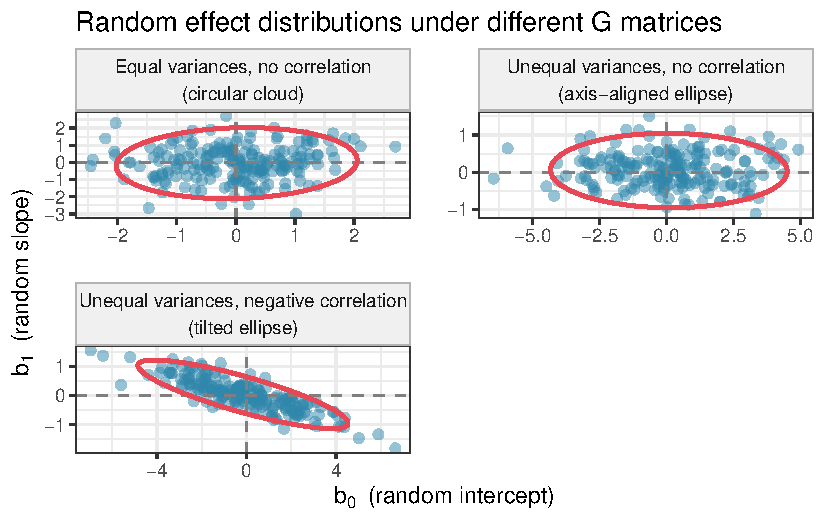
\includegraphics[width=0.9\textwidth,height=\textheight]{appendix-a-math_files/figure-pdf/re-distribution-plot-1.pdf}
\end{center}

\subsection{\texorpdfstring{What \(\mathbf{G}\) Is
Not}{What \textbackslash mathbf\{G\} Is Not}}\label{what-mathbfg-is-not}

Two common misconceptions are worth correcting explicitly.

\textbf{\(\mathbf{G}\) is not known in advance.} It is estimated from
the data, along with \(\boldsymbol{\beta}\) and
\(\sigma^2_\varepsilon\). The estimated \(\hat{\mathbf{G}}\) appears in
the random effects section of the model summary. With few groups, the
estimates will be uncertain --- especially the off-diagonal covariance,
which requires sufficient spread in both dimensions to estimate
reliably.

\textbf{\(\mathbf{G}\) is not the same as the residual covariance
matrix.} \(\mathbf{G}\) describes the distribution of random effects
across groups --- between-group variation. The residual variance
\(\sigma^2_\varepsilon\) describes the variation within groups after
accounting for the fixed and random effects. These are separate variance
components at different levels of the hierarchy, as discussed in Section
9.2.

\chapter{Datasets and R Packages}\label{sec-appendix-b}

This appendix documents all datasets and R packages used throughout the
book. All datasets are simulated with fixed random seeds for full
reproducibility --- every reader running the code will obtain identical
results. All datasets are saved as \texttt{.rds} files in the
\texttt{RDS/} directory of the book's companion repository and can be
loaded directly into R without re-running the simulation code.

The companion repository is available at:
\textbf{\url{https://github.com/Ebedthan/maov_data}}

\section{B.1 Datasets}\label{b.1-datasets}

\subsection{How to Load the Datasets}\label{how-to-load-the-datasets}

Each dataset can be loaded directly from the repository once you have
cloned it locally:

\begin{Shaded}
\begin{Highlighting}[]
\CommentTok{\# Load any dataset by name}
\NormalTok{systolic }\OtherTok{\textless{}{-}} \FunctionTok{readRDS}\NormalTok{(}\StringTok{"RDS/systolic.rds"}\NormalTok{)}
\NormalTok{gxe }\OtherTok{\textless{}{-}} \FunctionTok{readRDS}\NormalTok{(}\StringTok{"RDS/gxe.rds"}\NormalTok{)}
\NormalTok{cardiac\_recovery }\OtherTok{\textless{}{-}} \FunctionTok{readRDS}\NormalTok{(}\StringTok{"RDS/cardiac\_recovery.rds"}\NormalTok{)}
\NormalTok{cardiac\_recovery\_wide }\OtherTok{\textless{}{-}} \FunctionTok{readRDS}\NormalTok{(}\StringTok{"RDS/cardiac\_recovery\_wide.rds"}\NormalTok{)}
\NormalTok{grazing }\OtherTok{\textless{}{-}} \FunctionTok{readRDS}\NormalTok{(}\StringTok{"RDS/grazing.rds"}\NormalTok{)}
\NormalTok{irrigation }\OtherTok{\textless{}{-}} \FunctionTok{readRDS}\NormalTok{(}\StringTok{"RDS/irrigation.rds"}\NormalTok{)}
\NormalTok{physio }\OtherTok{\textless{}{-}} \FunctionTok{readRDS}\NormalTok{(}\StringTok{"RDS/physio.rds"}\NormalTok{)}
\NormalTok{birds }\OtherTok{\textless{}{-}} \FunctionTok{readRDS}\NormalTok{(}\StringTok{"RDS/birds.rds"}\NormalTok{)}
\end{Highlighting}
\end{Shaded}

Or regenerate any dataset from scratch by running the corresponding
simulation chunk. All chunks use \texttt{set.seed(42)} for
reproducibility.

\subsection{Dataset 1: Antihypertensive Drug Trial}\label{sec-systolic}

\textbf{File:} \texttt{RDS/systolic.rds}

\textbf{Used in:} Chapter \ref{sec-chap3} (One-Way ANOVA), Chapter
\ref{sec-chap4} (Multiple Comparisons)

\textbf{Description:} A simulated randomised controlled trial
investigating the effect of antihypertensive treatment on systolic blood
pressure in patients with mild hypertension. Patients are randomly
assigned to one of three groups: placebo, low-dose drug, or high-dose
drug, and systolic blood pressure (mmHg) is measured after eight weeks
of treatment.

\textbf{Design:} One-way completely randomised design. Three treatment
groups, 20 patients per group, \(N = 60\) observations total.

\textbf{Variables:}

\begin{longtable}[]{@{}lll@{}}
\toprule\noalign{}
Variable & Type & Description \\
\midrule\noalign{}
\endhead
\bottomrule\noalign{}
\endlastfoot
\texttt{bp} & Numeric & Systolic blood pressure (mmHg) \\
\texttt{group} & Factor & Treatment group (Placebo / Low dose / High
dose) \\
\end{longtable}

\textbf{True parameters:} group means 150, 140, and 128 mmHg; common
within-group SD = 12 mmHg.

\begin{Shaded}
\begin{Highlighting}[]
\FunctionTok{set.seed}\NormalTok{(}\DecValTok{42}\NormalTok{)}

\NormalTok{n         }\OtherTok{\textless{}{-}} \DecValTok{20}
\NormalTok{groups    }\OtherTok{\textless{}{-}} \FunctionTok{c}\NormalTok{(}\StringTok{"Placebo"}\NormalTok{, }\StringTok{"Low dose"}\NormalTok{, }\StringTok{"High dose"}\NormalTok{)}
\NormalTok{means     }\OtherTok{\textless{}{-}} \FunctionTok{c}\NormalTok{(}\DecValTok{150}\NormalTok{, }\DecValTok{140}\NormalTok{, }\DecValTok{128}\NormalTok{)}
\NormalTok{sd\_common }\OtherTok{\textless{}{-}} \DecValTok{12}

\NormalTok{group    }\OtherTok{\textless{}{-}} \FunctionTok{factor}\NormalTok{(}\FunctionTok{rep}\NormalTok{(groups, }\AttributeTok{each =}\NormalTok{ n), }\AttributeTok{levels =}\NormalTok{ groups)}
\NormalTok{bp       }\OtherTok{\textless{}{-}} \FunctionTok{c}\NormalTok{(}\FunctionTok{rnorm}\NormalTok{(n, }\AttributeTok{mean =}\NormalTok{ means[}\DecValTok{1}\NormalTok{], }\AttributeTok{sd =}\NormalTok{ sd\_common),}
              \FunctionTok{rnorm}\NormalTok{(n, }\AttributeTok{mean =}\NormalTok{ means[}\DecValTok{2}\NormalTok{], }\AttributeTok{sd =}\NormalTok{ sd\_common),}
              \FunctionTok{rnorm}\NormalTok{(n, }\AttributeTok{mean =}\NormalTok{ means[}\DecValTok{3}\NormalTok{], }\AttributeTok{sd =}\NormalTok{ sd\_common))}
\NormalTok{systolic }\OtherTok{\textless{}{-}} \FunctionTok{data.frame}\NormalTok{(bp, group)}

\FunctionTok{saveRDS}\NormalTok{(systolic, }\StringTok{"RDS/systolic.rds"}\NormalTok{)}
\FunctionTok{summary}\NormalTok{(systolic)}
\end{Highlighting}
\end{Shaded}

\begin{verbatim}
#>        bp               group   
#>  Min.   : 92.08   Placebo  :20  
#>  1st Qu.:129.61   Low dose :20  
#>  Median :136.62   High dose:20  
#>  Mean   :139.01                 
#>  3rd Qu.:148.76                 
#>  Max.   :177.44
\end{verbatim}

\subsection{Dataset 2: Genotype × Environment Wheat
Trial}\label{sec-gxe}

\textbf{File:} \texttt{RDS/gxe.rds}

\textbf{Used in:} Chapter \ref{sec-chap5} (Two-Way ANOVA and Factorial
Designs)

\textbf{Description:} A simulated multi-environment wheat trial designed
to demonstrate genotype × environment interaction (G×E). Four wheat
varieties are grown across three rainfall environments (dry, moderate,
wet), with five replicate plots per variety-environment combination. Two
varieties are environment-specific specialists (Var B thrives in wet
conditions; Var C in dry conditions), while two are stable generalists
(Var A and Var D), producing a clear crossover interaction.

\textbf{Design:} Two-way factorial design (variety × environment) with
replication. \(4 \times 3 \times 5 = 60\) observations total.

\textbf{Variables:}

\begin{longtable}[]{@{}lll@{}}
\toprule\noalign{}
Variable & Type & Description \\
\midrule\noalign{}
\endhead
\bottomrule\noalign{}
\endlastfoot
\texttt{variety} & Factor & Wheat variety (Var A / Var B / Var C / Var
D) \\
\texttt{env} & Factor & Growing environment (Dry / Moderate / Wet) \\
\texttt{rep} & Integer & Replicate number within each cell (1---5) \\
\texttt{yield} & Numeric & Plot yield (g/plot) \\
\end{longtable}

\textbf{True parameters:} cell means range from 40 (Var B in dry) to 65
(Var B in wet); within-cell SD = 5 g/plot.

\begin{Shaded}
\begin{Highlighting}[]
\FunctionTok{set.seed}\NormalTok{(}\DecValTok{42}\NormalTok{)}

\NormalTok{n\_rep     }\OtherTok{\textless{}{-}} \DecValTok{5}
\NormalTok{varieties }\OtherTok{\textless{}{-}} \FunctionTok{c}\NormalTok{(}\StringTok{"Var A"}\NormalTok{, }\StringTok{"Var B"}\NormalTok{, }\StringTok{"Var C"}\NormalTok{, }\StringTok{"Var D"}\NormalTok{)}
\NormalTok{envs      }\OtherTok{\textless{}{-}} \FunctionTok{c}\NormalTok{(}\StringTok{"Dry"}\NormalTok{, }\StringTok{"Moderate"}\NormalTok{, }\StringTok{"Wet"}\NormalTok{)}

\NormalTok{cell\_means }\OtherTok{\textless{}{-}} \FunctionTok{matrix}\NormalTok{(}
  \FunctionTok{c}\NormalTok{(}\DecValTok{50}\NormalTok{, }\DecValTok{52}\NormalTok{, }\DecValTok{51}\NormalTok{,}
    \DecValTok{40}\NormalTok{, }\DecValTok{52}\NormalTok{, }\DecValTok{65}\NormalTok{,}
    \DecValTok{62}\NormalTok{, }\DecValTok{53}\NormalTok{, }\DecValTok{41}\NormalTok{,}
    \DecValTok{50}\NormalTok{, }\DecValTok{51}\NormalTok{, }\DecValTok{50}\NormalTok{),}
  \AttributeTok{nrow =} \DecValTok{4}\NormalTok{, }\AttributeTok{byrow =} \ConstantTok{TRUE}\NormalTok{,}
  \AttributeTok{dimnames =} \FunctionTok{list}\NormalTok{(varieties, envs)}
\NormalTok{)}

\NormalTok{gxe        }\OtherTok{\textless{}{-}} \FunctionTok{expand.grid}\NormalTok{(}\AttributeTok{variety =}\NormalTok{ varieties,}
                           \AttributeTok{env     =}\NormalTok{ envs,}
                           \AttributeTok{rep     =} \FunctionTok{seq\_len}\NormalTok{(n\_rep))}
\NormalTok{gxe}\SpecialCharTok{$}\NormalTok{yield  }\OtherTok{\textless{}{-}} \FunctionTok{mapply}\NormalTok{(}\ControlFlowTok{function}\NormalTok{(v, e) \{}
  \FunctionTok{rnorm}\NormalTok{(}\DecValTok{1}\NormalTok{, }\AttributeTok{mean =}\NormalTok{ cell\_means[v, e], }\AttributeTok{sd =} \DecValTok{5}\NormalTok{)}
\NormalTok{\}, }\FunctionTok{as.character}\NormalTok{(gxe}\SpecialCharTok{$}\NormalTok{variety), }\FunctionTok{as.character}\NormalTok{(gxe}\SpecialCharTok{$}\NormalTok{env))}
\NormalTok{gxe}\SpecialCharTok{$}\NormalTok{variety }\OtherTok{\textless{}{-}} \FunctionTok{factor}\NormalTok{(gxe}\SpecialCharTok{$}\NormalTok{variety, }\AttributeTok{levels =}\NormalTok{ varieties)}
\NormalTok{gxe}\SpecialCharTok{$}\NormalTok{env     }\OtherTok{\textless{}{-}} \FunctionTok{factor}\NormalTok{(gxe}\SpecialCharTok{$}\NormalTok{env,     }\AttributeTok{levels =}\NormalTok{ envs)}

\FunctionTok{saveRDS}\NormalTok{(gxe, }\StringTok{"RDS/gxe.rds"}\NormalTok{)}
\FunctionTok{summary}\NormalTok{(gxe)}
\end{Highlighting}
\end{Shaded}

\begin{verbatim}
#>   variety         env          rep        yield      
#>  Var A:15   Dry     :20   Min.   :1   Min.   :26.03  
#>  Var B:15   Moderate:20   1st Qu.:2   1st Qu.:45.60  
#>  Var C:15   Wet     :20   Median :3   Median :52.71  
#>  Var D:15                 Mean   :3   Mean   :51.28  
#>                           3rd Qu.:4   3rd Qu.:56.95  
#>                           Max.   :5   Max.   :67.16
\end{verbatim}

\subsection{Dataset 3: Cardiac Rehabilitation
Trial}\label{sec-cardiac-recovery}

\textbf{Files:} \texttt{RDS/cardiac\_recovery.rds} (long format),
\texttt{RDS/cardiac\_recovery\_wide.rds} (wide format) \textbf{Used in:}
Chapter \ref{sec-chap6} (Repeated Measures ANOVA), Chapter
\ref{sec-chap9} (Mixed-Effects Models)

\textbf{Description:} A simulated longitudinal clinical trial following
40 patients recovering from cardiac surgery. Patients are randomly
assigned to either a standard rehabilitation programme (control) or an
intensive cardiac rehabilitation programme (intervention). Resting heart
rate (bpm) is measured at baseline and at weeks 4, 8, and 12. The
intensive programme produces a steeper decline in heart rate, creating a
significant group-by-time interaction.

\textbf{Design:} Mixed repeated measures design. Two between-subjects
groups (20 patients per group) crossed with four within-subject time
points. Total: 160 observations in long format.

\textbf{Variables (long format):}

\begin{longtable}[]{@{}lll@{}}
\toprule\noalign{}
Variable & Type & Description \\
\midrule\noalign{}
\endhead
\bottomrule\noalign{}
\endlastfoot
\texttt{hr} & Numeric & Resting heart rate (bpm) \\
\texttt{group} & Factor & Rehabilitation programme (Control /
Intervention) \\
\texttt{time} & Factor & Measurement time point (0 / 4 / 8 / 12
weeks) \\
\texttt{subject} & Factor & Patient identifier (1---40) \\
\end{longtable}

\textbf{True parameters:} control trajectory (82, 80, 78, 77 bpm);
intervention trajectory (82, 76, 71, 68 bpm); within-subject covariance
with moderate temporal correlation.

\begin{Shaded}
\begin{Highlighting}[]
\FunctionTok{library}\NormalTok{(MASS)}
\FunctionTok{set.seed}\NormalTok{(}\DecValTok{42}\NormalTok{)}

\NormalTok{n\_group            }\OtherTok{\textless{}{-}} \DecValTok{20}
\NormalTok{k                  }\OtherTok{\textless{}{-}} \DecValTok{4}
\NormalTok{times              }\OtherTok{\textless{}{-}} \FunctionTok{c}\NormalTok{(}\DecValTok{0}\NormalTok{, }\DecValTok{4}\NormalTok{, }\DecValTok{8}\NormalTok{, }\DecValTok{12}\NormalTok{)}
\NormalTok{groups             }\OtherTok{\textless{}{-}} \FunctionTok{c}\NormalTok{(}\StringTok{"Control"}\NormalTok{, }\StringTok{"Intervention"}\NormalTok{)}
\NormalTok{means\_control      }\OtherTok{\textless{}{-}} \FunctionTok{c}\NormalTok{(}\DecValTok{82}\NormalTok{, }\DecValTok{80}\NormalTok{, }\DecValTok{78}\NormalTok{, }\DecValTok{77}\NormalTok{)}
\NormalTok{means\_intervention }\OtherTok{\textless{}{-}} \FunctionTok{c}\NormalTok{(}\DecValTok{82}\NormalTok{, }\DecValTok{76}\NormalTok{, }\DecValTok{71}\NormalTok{, }\DecValTok{68}\NormalTok{)}

\NormalTok{sigma\_within }\OtherTok{\textless{}{-}} \FunctionTok{matrix}\NormalTok{(}\FunctionTok{c}\NormalTok{(}\DecValTok{16}\NormalTok{,}\DecValTok{8}\NormalTok{,}\DecValTok{6}\NormalTok{,}\DecValTok{4}\NormalTok{, }\DecValTok{8}\NormalTok{,}\DecValTok{16}\NormalTok{,}\DecValTok{8}\NormalTok{,}\DecValTok{6}\NormalTok{,}
                          \DecValTok{6}\NormalTok{,}\DecValTok{8}\NormalTok{,}\DecValTok{16}\NormalTok{,}\DecValTok{8}\NormalTok{, }\DecValTok{4}\NormalTok{,}\DecValTok{6}\NormalTok{,}\DecValTok{8}\NormalTok{,}\DecValTok{16}\NormalTok{), }\AttributeTok{nrow =} \DecValTok{4}\NormalTok{)}

\NormalTok{df\_control      }\OtherTok{\textless{}{-}} \FunctionTok{as.data.frame}\NormalTok{(}
  \FunctionTok{mvrnorm}\NormalTok{(n\_group, }\AttributeTok{mu =}\NormalTok{ means\_control,      }\AttributeTok{Sigma =}\NormalTok{ sigma\_within))}
\NormalTok{df\_intervention }\OtherTok{\textless{}{-}} \FunctionTok{as.data.frame}\NormalTok{(}
  \FunctionTok{mvrnorm}\NormalTok{(n\_group, }\AttributeTok{mu =}\NormalTok{ means\_intervention, }\AttributeTok{Sigma =}\NormalTok{ sigma\_within))}
\FunctionTok{names}\NormalTok{(df\_control) }\OtherTok{\textless{}{-}} \FunctionTok{names}\NormalTok{(df\_intervention) }\OtherTok{\textless{}{-}} \FunctionTok{paste0}\NormalTok{(}\StringTok{"t"}\NormalTok{, }\DecValTok{1}\SpecialCharTok{:}\NormalTok{k)}

\NormalTok{df\_wide          }\OtherTok{\textless{}{-}} \FunctionTok{rbind}\NormalTok{(df\_control, df\_intervention)}
\NormalTok{df\_wide}\SpecialCharTok{$}\NormalTok{subject  }\OtherTok{\textless{}{-}} \FunctionTok{factor}\NormalTok{(}\DecValTok{1}\SpecialCharTok{:}\NormalTok{(}\DecValTok{2} \SpecialCharTok{*}\NormalTok{ n\_group))}
\NormalTok{df\_wide}\SpecialCharTok{$}\NormalTok{group    }\OtherTok{\textless{}{-}} \FunctionTok{factor}\NormalTok{(}\FunctionTok{rep}\NormalTok{(groups, }\AttributeTok{each =}\NormalTok{ n\_group),}
                            \AttributeTok{levels =}\NormalTok{ groups)}

\NormalTok{cardiac\_recovery\_wide }\OtherTok{\textless{}{-}}\NormalTok{ df\_wide}
\NormalTok{cardiac\_recovery      }\OtherTok{\textless{}{-}} \FunctionTok{reshape}\NormalTok{(}
\NormalTok{  df\_wide, }\AttributeTok{varying =} \FunctionTok{paste0}\NormalTok{(}\StringTok{"t"}\NormalTok{, }\DecValTok{1}\SpecialCharTok{:}\NormalTok{k),}
  \AttributeTok{v.names =} \StringTok{"hr"}\NormalTok{, }\AttributeTok{timevar =} \StringTok{"time"}\NormalTok{, }\AttributeTok{times =}\NormalTok{ times,}
  \AttributeTok{direction =} \StringTok{"long"}\NormalTok{)}
\NormalTok{cardiac\_recovery}\SpecialCharTok{$}\NormalTok{time    }\OtherTok{\textless{}{-}} \FunctionTok{factor}\NormalTok{(cardiac\_recovery}\SpecialCharTok{$}\NormalTok{time)}
\NormalTok{cardiac\_recovery}\SpecialCharTok{$}\NormalTok{subject }\OtherTok{\textless{}{-}} \FunctionTok{factor}\NormalTok{(cardiac\_recovery}\SpecialCharTok{$}\NormalTok{subject)}

\FunctionTok{saveRDS}\NormalTok{(cardiac\_recovery,      }\StringTok{"RDS/cardiac\_recovery.rds"}\NormalTok{)}
\FunctionTok{saveRDS}\NormalTok{(cardiac\_recovery\_wide, }\StringTok{"RDS/cardiac\_recovery\_wide.rds"}\NormalTok{)}
\FunctionTok{summary}\NormalTok{(cardiac\_recovery)}
\end{Highlighting}
\end{Shaded}

\begin{verbatim}
#>     subject             group    time          hr              id       
#>  1      :  4   Control     :80   0 :40   Min.   :58.80   Min.   : 1.00  
#>  2      :  4   Intervention:80   4 :40   1st Qu.:71.66   1st Qu.:10.75  
#>  3      :  4                     8 :40   Median :77.09   Median :20.50  
#>  4      :  4                     12:40   Mean   :76.32   Mean   :20.50  
#>  5      :  4                             3rd Qu.:80.38   3rd Qu.:30.25  
#>  6      :  4                             Max.   :93.61   Max.   :40.00  
#>  (Other):136
\end{verbatim}

\subsection{Dataset 4: Grazing Effects on Plant Species
Richness}\label{sec-grazing}

\textbf{File:} \texttt{RDS/grazing.rds}

\textbf{Used in:} Chapter \ref{sec-chap7} (Split-Plot and Nested
Designs)

\textbf{Description:} A simulated ecological experiment investigating
the effect of grazing intensity on plant species richness in a
grassland. Three grazing treatments (ungrazed, light, heavy) are applied
to six large paddocks (two per treatment). Within each paddock, species
richness is counted in four quadrats, creating a nested structure where
quadrats are subsamples within paddocks and paddocks are the true
experimental units.

\textbf{Design:} Nested design with two levels. Three treatments × 2
paddocks per treatment × 4 quadrats per paddock = 24 observations.

\textbf{Variables:}

\begin{longtable}[]{@{}lll@{}}
\toprule\noalign{}
Variable & Type & Description \\
\midrule\noalign{}
\endhead
\bottomrule\noalign{}
\endlastfoot
\texttt{richness} & Integer & Plant species richness per quadrat \\
\texttt{treatment} & Factor & Grazing intensity (Ungrazed / Light /
Heavy) \\
\texttt{paddock} & Factor & Paddock identifier (U1, U2, L1, L2, H1,
H2) \\
\end{longtable}

\textbf{True parameters:} treatment means 12, 9, and 6 species per
quadrat (ungrazed to heavy); paddock SD = 2; quadrat SD = 1.

\begin{Shaded}
\begin{Highlighting}[]
\FunctionTok{set.seed}\NormalTok{(}\DecValTok{42}\NormalTok{)}

\NormalTok{n\_treatments    }\OtherTok{\textless{}{-}} \DecValTok{3}
\NormalTok{n\_paddocks      }\OtherTok{\textless{}{-}} \DecValTok{2}
\NormalTok{n\_quadrats      }\OtherTok{\textless{}{-}} \DecValTok{4}
\NormalTok{treatment\_means }\OtherTok{\textless{}{-}} \FunctionTok{c}\NormalTok{(}\DecValTok{12}\NormalTok{, }\DecValTok{9}\NormalTok{, }\DecValTok{6}\NormalTok{)}
\NormalTok{paddock\_sd      }\OtherTok{\textless{}{-}} \DecValTok{2}
\NormalTok{quadrat\_sd      }\OtherTok{\textless{}{-}} \DecValTok{1}

\NormalTok{grazing }\OtherTok{\textless{}{-}} \FunctionTok{do.call}\NormalTok{(rbind, }\FunctionTok{lapply}\NormalTok{(}\FunctionTok{seq\_len}\NormalTok{(n\_treatments), }\ControlFlowTok{function}\NormalTok{(t) \{}
  \FunctionTok{do.call}\NormalTok{(rbind, }\FunctionTok{lapply}\NormalTok{(}\FunctionTok{seq\_len}\NormalTok{(n\_paddocks), }\ControlFlowTok{function}\NormalTok{(p) \{}
\NormalTok{    paddock\_effect }\OtherTok{\textless{}{-}} \FunctionTok{rnorm}\NormalTok{(}\DecValTok{1}\NormalTok{, }\DecValTok{0}\NormalTok{, paddock\_sd)}
    \FunctionTok{data.frame}\NormalTok{(}
      \AttributeTok{richness  =} \FunctionTok{round}\NormalTok{(}\FunctionTok{rnorm}\NormalTok{(n\_quadrats,}
                              \AttributeTok{mean =}\NormalTok{ treatment\_means[t] }\SpecialCharTok{+}
\NormalTok{                                     paddock\_effect,}
                              \AttributeTok{sd   =}\NormalTok{ quadrat\_sd)),}
      \AttributeTok{treatment =} \FunctionTok{factor}\NormalTok{(}\FunctionTok{c}\NormalTok{(}\StringTok{"Ungrazed"}\NormalTok{, }\StringTok{"Light"}\NormalTok{, }\StringTok{"Heavy"}\NormalTok{)[t],}
                         \AttributeTok{levels =} \FunctionTok{c}\NormalTok{(}\StringTok{"Ungrazed"}\NormalTok{, }\StringTok{"Light"}\NormalTok{, }\StringTok{"Heavy"}\NormalTok{)),}
      \AttributeTok{paddock   =} \FunctionTok{factor}\NormalTok{(}\FunctionTok{paste0}\NormalTok{(}\FunctionTok{c}\NormalTok{(}\StringTok{"U"}\NormalTok{,}\StringTok{"L"}\NormalTok{,}\StringTok{"H"}\NormalTok{)[t], p))}
\NormalTok{    )}
\NormalTok{  \}))}
\NormalTok{\}))}

\FunctionTok{saveRDS}\NormalTok{(grazing, }\StringTok{"RDS/grazing.rds"}\NormalTok{)}
\FunctionTok{summary}\NormalTok{(grazing)}
\end{Highlighting}
\end{Shaded}

\begin{verbatim}
#>     richness         treatment paddock
#>  Min.   : 3.000   Ungrazed:8   U1:4   
#>  1st Qu.: 6.750   Light   :8   U2:4   
#>  Median :10.500   Heavy   :8   L1:4   
#>  Mean   : 9.792                L2:4   
#>  3rd Qu.:13.250                H1:4   
#>  Max.   :15.000                H2:4
\end{verbatim}

\subsection{Dataset 5: Irrigation × Fertiliser Split-Plot
Trial}\label{sec-irrig}

\textbf{File:} \texttt{RDS/irrigation.rds}

\textbf{Used in:} Chapter \ref{sec-chap7} (Split-Plot and Nested
Designs)

\textbf{Description:} A simulated agricultural split-plot experiment
testing the effects of irrigation regime and fertiliser type on wheat
yield. Irrigation (rainfed vs irrigated) is the whole-plot factor
applied to entire fields; fertiliser type (none, nitrogen, phosphorus)
is the sub-plot factor applied to individual plots within each field.
The design correctly reflects the practical constraint that irrigation
infrastructure cannot be changed within a field, creating two different
error terms for the two factors.

\textbf{Design:} Split-plot design. Two irrigation treatments × 3 fields
per treatment × 3 fertiliser types per field = 18 observations.

\textbf{Variables:}

\begin{longtable}[]{@{}
  >{\raggedright\arraybackslash}p{(\columnwidth - 4\tabcolsep) * \real{0.3448}}
  >{\raggedright\arraybackslash}p{(\columnwidth - 4\tabcolsep) * \real{0.2069}}
  >{\raggedright\arraybackslash}p{(\columnwidth - 4\tabcolsep) * \real{0.4483}}@{}}
\toprule\noalign{}
\begin{minipage}[b]{\linewidth}\raggedright
Variable
\end{minipage} & \begin{minipage}[b]{\linewidth}\raggedright
Type
\end{minipage} & \begin{minipage}[b]{\linewidth}\raggedright
Description
\end{minipage} \\
\midrule\noalign{}
\endhead
\bottomrule\noalign{}
\endlastfoot
\texttt{yield} & Numeric & Wheat yield (g/plot) \\
\texttt{irrigation} & Factor & Irrigation regime (Rainfed /
Irrigated) \\
\texttt{fertiliser} & Factor & Fertiliser type (None / Nitrogen /
Phosphorus) \\
\texttt{field} & Factor & Field identifier (R1---R3 rainfed, I1---I3
irrigated) \\
\end{longtable}

\textbf{True parameters:} cell means range from 30 (rainfed, no
fertiliser) to 55 (irrigated, nitrogen); field SD = 4; plot SD = 2.

\begin{Shaded}
\begin{Highlighting}[]
\FunctionTok{set.seed}\NormalTok{(}\DecValTok{42}\NormalTok{)}

\NormalTok{irrigation }\OtherTok{\textless{}{-}} \FunctionTok{c}\NormalTok{(}\StringTok{"Rainfed"}\NormalTok{, }\StringTok{"Irrigated"}\NormalTok{)}
\NormalTok{fertiliser }\OtherTok{\textless{}{-}} \FunctionTok{c}\NormalTok{(}\StringTok{"None"}\NormalTok{, }\StringTok{"Nitrogen"}\NormalTok{, }\StringTok{"Phosphorus"}\NormalTok{)}
\NormalTok{n\_fields   }\OtherTok{\textless{}{-}} \DecValTok{3}

\NormalTok{cell\_means }\OtherTok{\textless{}{-}} \FunctionTok{matrix}\NormalTok{(}
  \FunctionTok{c}\NormalTok{(}\DecValTok{30}\NormalTok{, }\DecValTok{38}\NormalTok{, }\DecValTok{35}\NormalTok{, }\DecValTok{42}\NormalTok{, }\DecValTok{55}\NormalTok{, }\DecValTok{50}\NormalTok{), }\AttributeTok{nrow =} \DecValTok{2}\NormalTok{, }\AttributeTok{byrow =} \ConstantTok{TRUE}\NormalTok{,}
  \AttributeTok{dimnames =} \FunctionTok{list}\NormalTok{(irrigation, fertiliser))}

\NormalTok{df\_agr }\OtherTok{\textless{}{-}} \FunctionTok{do.call}\NormalTok{(rbind, }\FunctionTok{lapply}\NormalTok{(}\FunctionTok{seq\_along}\NormalTok{(irrigation), }\ControlFlowTok{function}\NormalTok{(i) \{}
  \FunctionTok{do.call}\NormalTok{(rbind, }\FunctionTok{lapply}\NormalTok{(}\FunctionTok{seq\_len}\NormalTok{(n\_fields), }\ControlFlowTok{function}\NormalTok{(f) \{}
\NormalTok{    field\_effect }\OtherTok{\textless{}{-}} \FunctionTok{rnorm}\NormalTok{(}\DecValTok{1}\NormalTok{, }\DecValTok{0}\NormalTok{, }\DecValTok{4}\NormalTok{)}
    \FunctionTok{data.frame}\NormalTok{(}
      \AttributeTok{yield      =} \FunctionTok{sapply}\NormalTok{(fertiliser, }\ControlFlowTok{function}\NormalTok{(fert)}
        \FunctionTok{rnorm}\NormalTok{(}\DecValTok{1}\NormalTok{, }\AttributeTok{mean =}\NormalTok{ cell\_means[i, fert] }\SpecialCharTok{+}\NormalTok{ field\_effect, }\AttributeTok{sd =} \DecValTok{2}\NormalTok{)),}
      \AttributeTok{irrigation =}\NormalTok{ irrigation[i],}
      \AttributeTok{fertiliser =}\NormalTok{ fertiliser,}
      \AttributeTok{field      =} \FunctionTok{factor}\NormalTok{(}\FunctionTok{paste0}\NormalTok{(}\FunctionTok{substr}\NormalTok{(irrigation[i], }\DecValTok{1}\NormalTok{, }\DecValTok{1}\NormalTok{), f))}
\NormalTok{    )}
\NormalTok{  \}))}
\NormalTok{\}))}

\NormalTok{df\_agr}\SpecialCharTok{$}\NormalTok{irrigation }\OtherTok{\textless{}{-}} \FunctionTok{factor}\NormalTok{(df\_agr}\SpecialCharTok{$}\NormalTok{irrigation,}
                              \AttributeTok{levels =} \FunctionTok{c}\NormalTok{(}\StringTok{"Rainfed"}\NormalTok{, }\StringTok{"Irrigated"}\NormalTok{))}
\NormalTok{df\_agr}\SpecialCharTok{$}\NormalTok{fertiliser }\OtherTok{\textless{}{-}} \FunctionTok{factor}\NormalTok{(df\_agr}\SpecialCharTok{$}\NormalTok{fertiliser, }\AttributeTok{levels =}\NormalTok{ fertiliser)}

\FunctionTok{saveRDS}\NormalTok{(df\_agr, }\StringTok{"RDS/irrigation.rds"}\NormalTok{)}
\FunctionTok{summary}\NormalTok{(df\_agr)}
\end{Highlighting}
\end{Shaded}

\begin{verbatim}
#>      yield           irrigation      fertiliser field 
#>  Min.   :31.40   Rainfed  :9    None      :6    R1:3  
#>  1st Qu.:36.62   Irrigated:9    Nitrogen  :6    R2:3  
#>  Median :43.43                  Phosphorus:6    R3:3  
#>  Mean   :42.98                                  I1:3  
#>  3rd Qu.:48.91                                  I2:3  
#>  Max.   :53.43                                  I3:3
\end{verbatim}

\subsection{Dataset 6: Physiotherapy Protocol: Three-Level Nested
Trial}\label{sec-physio}

\textbf{File:} \texttt{RDS/physio.rds}

\textbf{Used in:} Chapter \ref{sec-chap9} (Mixed-Effects Models)

\textbf{Description:} A simulated national health study investigating
the effect of a new physiotherapy protocol on functional recovery scores
following knee replacement surgery. Patients are recruited from 15
hospitals distributed across 3 regions, with 8-12 patients per hospital.
The three-level nested structure (patients within hospitals within
regions) requires a mixed-effects model with two nested random
intercepts to produce valid inference about the treatment effect.

\textbf{Design:} Three-level nested observational study. 3 regions × 5
hospitals per region × 8-12 patients per hospital. Total: 148 patients.

\textbf{Variables:}

\begin{longtable}[]{@{}lll@{}}
\toprule\noalign{}
Variable & Type & Description \\
\midrule\noalign{}
\endhead
\bottomrule\noalign{}
\endlastfoot
\texttt{recovery} & Numeric & Functional recovery score (0---100) \\
\texttt{treatment} & Factor & Protocol (Control / Treatment) \\
\texttt{hospital} & Factor & Hospital identifier (H11---H35) \\
\texttt{region} & Factor & Region identifier (R1 / R2 / R3) \\
\end{longtable}

\textbf{True parameters:} treatment effect = 7 points; region SD = 4;
hospital-within-region SD = 3; patient-level SD = 8.

\begin{Shaded}
\begin{Highlighting}[]
\FunctionTok{set.seed}\NormalTok{(}\DecValTok{42}\NormalTok{)}

\NormalTok{n\_regions        }\OtherTok{\textless{}{-}} \DecValTok{3}
\NormalTok{n\_hospitals      }\OtherTok{\textless{}{-}} \DecValTok{5}
\NormalTok{n\_patients       }\OtherTok{\textless{}{-}} \FunctionTok{c}\NormalTok{(}\DecValTok{8}\NormalTok{, }\DecValTok{9}\NormalTok{, }\DecValTok{10}\NormalTok{, }\DecValTok{11}\NormalTok{, }\DecValTok{12}\NormalTok{)}
\NormalTok{treatment\_effect }\OtherTok{\textless{}{-}} \DecValTok{7}

\NormalTok{df\_nested }\OtherTok{\textless{}{-}} \FunctionTok{do.call}\NormalTok{(rbind, }\FunctionTok{lapply}\NormalTok{(}\FunctionTok{seq\_len}\NormalTok{(n\_regions), }\ControlFlowTok{function}\NormalTok{(r) \{}
\NormalTok{  region\_effect }\OtherTok{\textless{}{-}} \FunctionTok{rnorm}\NormalTok{(}\DecValTok{1}\NormalTok{, }\DecValTok{0}\NormalTok{, }\DecValTok{4}\NormalTok{)}
  \FunctionTok{do.call}\NormalTok{(rbind, }\FunctionTok{lapply}\NormalTok{(}\FunctionTok{seq\_len}\NormalTok{(n\_hospitals), }\ControlFlowTok{function}\NormalTok{(h) \{}
\NormalTok{    hospital\_effect }\OtherTok{\textless{}{-}} \FunctionTok{rnorm}\NormalTok{(}\DecValTok{1}\NormalTok{, }\DecValTok{0}\NormalTok{, }\DecValTok{3}\NormalTok{)}
\NormalTok{    n\_pat   }\OtherTok{\textless{}{-}} \FunctionTok{sample}\NormalTok{(n\_patients, }\DecValTok{1}\NormalTok{)}
\NormalTok{    treatment }\OtherTok{\textless{}{-}} \FunctionTok{rep}\NormalTok{(}\FunctionTok{c}\NormalTok{(}\StringTok{"Control"}\NormalTok{, }\StringTok{"Treatment"}\NormalTok{), }\AttributeTok{length.out =}\NormalTok{ n\_pat)}
    \FunctionTok{data.frame}\NormalTok{(}
      \AttributeTok{recovery  =} \FunctionTok{rnorm}\NormalTok{(n\_pat,}
                        \AttributeTok{mean =} \DecValTok{60} \SpecialCharTok{+}\NormalTok{ region\_effect }\SpecialCharTok{+}
\NormalTok{                               hospital\_effect }\SpecialCharTok{+}
\NormalTok{                               treatment\_effect }\SpecialCharTok{*}
\NormalTok{                               (treatment }\SpecialCharTok{==} \StringTok{"Treatment"}\NormalTok{),}
                        \AttributeTok{sd   =} \DecValTok{8}\NormalTok{),}
      \AttributeTok{treatment =} \FunctionTok{factor}\NormalTok{(treatment,}
                         \AttributeTok{levels =} \FunctionTok{c}\NormalTok{(}\StringTok{"Control"}\NormalTok{, }\StringTok{"Treatment"}\NormalTok{)),}
      \AttributeTok{hospital  =} \FunctionTok{factor}\NormalTok{(}\FunctionTok{paste0}\NormalTok{(}\StringTok{"H"}\NormalTok{, r, h)),}
      \AttributeTok{region    =} \FunctionTok{factor}\NormalTok{(}\FunctionTok{paste0}\NormalTok{(}\StringTok{"R"}\NormalTok{, r))}
\NormalTok{    )}
\NormalTok{  \}))}
\NormalTok{\}))}

\FunctionTok{saveRDS}\NormalTok{(df\_nested, }\StringTok{"RDS/physio.rds"}\NormalTok{)}
\FunctionTok{summary}\NormalTok{(df\_nested)}
\end{Highlighting}
\end{Shaded}

\begin{verbatim}
#>     recovery         treatment     hospital  region 
#>  Min.   :39.19   Control  :78   H14    :12   R1:52  
#>  1st Qu.:57.59   Treatment:70   H23    :12   R2:45  
#>  Median :64.79                  H34    :12   R3:51  
#>  Mean   :64.38                  H12    :11          
#>  3rd Qu.:72.37                  H13    :11          
#>  Max.   :95.10                  H32    :11          
#>                                 (Other):79
\end{verbatim}

\begin{center}\rule{0.5\linewidth}{0.5pt}\end{center}

\subsection{Dataset 7: Bird Abundance in Forest
Landscapes}\label{sec-birds}

\textbf{File:} \texttt{RDS/birds.rds}

\textbf{Used in:} Chapter \ref{sec-chap11} (Generalised Linear Mixed
Models)

\textbf{Description:} A simulated ecological survey of bird abundance
across three landscape types (agricultural matrix, fragmented forest,
and continuous forest). The focal species is a forest interior
specialist that is genuinely absent from many agricultural sites
(structural zeros), creating a zero-inflated count response that
motivates the use of negative binomial and zero-inflated GLMMs. Five
transects are surveyed within each of 24 sites (8 per landscape type).

\textbf{Design:} Hierarchical count survey. 3 landscape types × 8 sites
per landscape × 5 transects per site = 120 observations.

\textbf{Variables:}

\begin{longtable}[]{@{}
  >{\raggedright\arraybackslash}p{(\columnwidth - 4\tabcolsep) * \real{0.3448}}
  >{\raggedright\arraybackslash}p{(\columnwidth - 4\tabcolsep) * \real{0.2069}}
  >{\raggedright\arraybackslash}p{(\columnwidth - 4\tabcolsep) * \real{0.4483}}@{}}
\toprule\noalign{}
\begin{minipage}[b]{\linewidth}\raggedright
Variable
\end{minipage} & \begin{minipage}[b]{\linewidth}\raggedright
Type
\end{minipage} & \begin{minipage}[b]{\linewidth}\raggedright
Description
\end{minipage} \\
\midrule\noalign{}
\endhead
\bottomrule\noalign{}
\endlastfoot
\texttt{count} & Integer & Number of individuals detected per
transect \\
\texttt{landscape} & Factor & Landscape type (Agricultural / Fragmented
/ Continuous) \\
\texttt{site} & Factor & Site identifier (Agr1---Agr8, Fra1---Fra8,
Con1---Con8) \\
\texttt{transect} & Factor & Transect number within site (1---5) \\
\end{longtable}

\textbf{True parameters:} structural absence probabilities of 0.70
(agricultural), 0.30 (fragmented), and 0.00 (continuous); expected
log-counts of 1.2, 2.2, and 3.2 given presence; negative binomial size =
2; site SD = 0.5 on log scale.

\begin{Shaded}
\begin{Highlighting}[]
\FunctionTok{set.seed}\NormalTok{(}\DecValTok{42}\NormalTok{)}

\NormalTok{n\_landscapes    }\OtherTok{\textless{}{-}} \DecValTok{3}
\NormalTok{n\_sites         }\OtherTok{\textless{}{-}} \DecValTok{8}
\NormalTok{n\_transects     }\OtherTok{\textless{}{-}} \DecValTok{5}
\NormalTok{landscape\_names }\OtherTok{\textless{}{-}} \FunctionTok{c}\NormalTok{(}\StringTok{"Agricultural"}\NormalTok{, }\StringTok{"Fragmented"}\NormalTok{, }\StringTok{"Continuous"}\NormalTok{)}
\NormalTok{zi\_prob         }\OtherTok{\textless{}{-}} \FunctionTok{c}\NormalTok{(}\FloatTok{0.70}\NormalTok{, }\FloatTok{0.30}\NormalTok{, }\FloatTok{0.00}\NormalTok{)}
\NormalTok{lambda\_log      }\OtherTok{\textless{}{-}} \FunctionTok{c}\NormalTok{(}\FloatTok{1.2}\NormalTok{, }\FloatTok{2.2}\NormalTok{, }\FloatTok{3.2}\NormalTok{)}
\NormalTok{site\_sd         }\OtherTok{\textless{}{-}} \FloatTok{0.5}

\NormalTok{df\_birds }\OtherTok{\textless{}{-}} \FunctionTok{do.call}\NormalTok{(rbind, }\FunctionTok{lapply}\NormalTok{(}
  \FunctionTok{seq\_len}\NormalTok{(n\_landscapes), }\ControlFlowTok{function}\NormalTok{(l) \{}
  \FunctionTok{do.call}\NormalTok{(rbind, }\FunctionTok{lapply}\NormalTok{(}\FunctionTok{seq\_len}\NormalTok{(n\_sites), }\ControlFlowTok{function}\NormalTok{(s) \{}
\NormalTok{    site\_effect  }\OtherTok{\textless{}{-}} \FunctionTok{rnorm}\NormalTok{(}\DecValTok{1}\NormalTok{, }\DecValTok{0}\NormalTok{, site\_sd)}
\NormalTok{    site\_absent  }\OtherTok{\textless{}{-}} \FunctionTok{rbinom}\NormalTok{(}\DecValTok{1}\NormalTok{, }\DecValTok{1}\NormalTok{, }\AttributeTok{prob =}\NormalTok{ zi\_prob[l])}
\NormalTok{    counts }\OtherTok{\textless{}{-}} \ControlFlowTok{if}\NormalTok{ (site\_absent }\SpecialCharTok{==} \DecValTok{1}\NormalTok{) \{}
      \FunctionTok{rep}\NormalTok{(}\DecValTok{0}\NormalTok{, n\_transects)}
\NormalTok{    \} }\ControlFlowTok{else}\NormalTok{ \{}
      \FunctionTok{rnbinom}\NormalTok{(n\_transects,}
              \AttributeTok{mu   =} \FunctionTok{exp}\NormalTok{(lambda\_log[l] }\SpecialCharTok{+}\NormalTok{ site\_effect),}
              \AttributeTok{size =} \DecValTok{2}\NormalTok{)}
\NormalTok{    \}}
    \FunctionTok{data.frame}\NormalTok{(}
      \AttributeTok{count     =}\NormalTok{ counts,}
      \AttributeTok{landscape =} \FunctionTok{factor}\NormalTok{(landscape\_names[l],}
                         \AttributeTok{levels =}\NormalTok{ landscape\_names),}
      \AttributeTok{site      =} \FunctionTok{factor}\NormalTok{(}\FunctionTok{paste0}\NormalTok{(}
        \FunctionTok{substr}\NormalTok{(landscape\_names[l], }\DecValTok{1}\NormalTok{, }\DecValTok{3}\NormalTok{), s)),}
      \AttributeTok{transect  =} \FunctionTok{factor}\NormalTok{(}\DecValTok{1}\SpecialCharTok{:}\NormalTok{n\_transects)}
\NormalTok{    )}
\NormalTok{  \}))}
\NormalTok{\}))}

\FunctionTok{saveRDS}\NormalTok{(df\_birds, }\StringTok{"RDS/birds.rds"}\NormalTok{)}
\FunctionTok{summary}\NormalTok{(df\_birds)}
\end{Highlighting}
\end{Shaded}

\begin{verbatim}
#>      count               landscape       site    transect
#>  Min.   : 0.000   Agricultural:40   Agr1   : 5   1:24    
#>  1st Qu.: 0.000   Fragmented  :40   Agr2   : 5   2:24    
#>  Median : 5.000   Continuous  :40   Agr3   : 5   3:24    
#>  Mean   : 8.925                     Agr4   : 5   4:24    
#>  3rd Qu.:14.000                     Agr5   : 5   5:24    
#>  Max.   :47.000                     Agr6   : 5           
#>                                     (Other):90
\end{verbatim}

\subsection{Dataset Summary Table}\label{dataset-summary-table}

\begin{longtable}[]{@{}
  >{\raggedright\arraybackslash}p{(\columnwidth - 10\tabcolsep) * \real{0.1915}}
  >{\raggedright\arraybackslash}p{(\columnwidth - 10\tabcolsep) * \real{0.1277}}
  >{\raggedright\arraybackslash}p{(\columnwidth - 10\tabcolsep) * \real{0.1702}}
  >{\raggedright\arraybackslash}p{(\columnwidth - 10\tabcolsep) * \real{0.1064}}
  >{\raggedright\arraybackslash}p{(\columnwidth - 10\tabcolsep) * \real{0.2128}}
  >{\raggedright\arraybackslash}p{(\columnwidth - 10\tabcolsep) * \real{0.1915}}@{}}
\toprule\noalign{}
\begin{minipage}[b]{\linewidth}\raggedright
Dataset
\end{minipage} & \begin{minipage}[b]{\linewidth}\raggedright
File
\end{minipage} & \begin{minipage}[b]{\linewidth}\raggedright
Design
\end{minipage} & \begin{minipage}[b]{\linewidth}\raggedright
\(N\)
\end{minipage} & \begin{minipage}[b]{\linewidth}\raggedright
Response
\end{minipage} & \begin{minipage}[b]{\linewidth}\raggedright
Chapter
\end{minipage} \\
\midrule\noalign{}
\endhead
\bottomrule\noalign{}
\endlastfoot
Antihypertensive trial & \texttt{systolic.rds} & One-way CRD & 60 &
Blood pressure (mmHg) & 3, 4 \\
G×E wheat trial & \texttt{gxe.rds} & Two-way factorial & 60 & Yield
(g/plot) & 5 \\
Cardiac rehabilitation & \texttt{cardiac\_recovery.rds} & Repeated
measures & 160 & Heart rate (bpm) & 6, 9 \\
Grazing richness & \texttt{grazing.rds} & Nested & 24 & Species richness
& 7 \\
Irrigation × fertiliser & \texttt{irrigation.rds} & Split-plot & 18 &
Yield (g/plot) & 7 \\
Physiotherapy trial & \texttt{physio.rds} & Three-level nested & 148 &
Recovery score & 9 \\
Bird abundance & \texttt{birds.rds} & Count survey & 120 & Individual
count & 11 \\
\end{longtable}

\section{B.2 R Packages}\label{b.2-r-packages}

All analyses in this book were conducted in R v3.6.0 \citep{R2026}. The
following packages are required to reproduce all code in the book.
Install them all at once with:

\begin{Shaded}
\begin{Highlighting}[]
\NormalTok{packages }\OtherTok{\textless{}{-}} \FunctionTok{c}\NormalTok{(}
  \CommentTok{\# Core modelling}
  \StringTok{"lme4"}\NormalTok{, }\StringTok{"lmerTest"}\NormalTok{, }\StringTok{"nlme"}\NormalTok{, }\StringTok{"glmmTMB"}\NormalTok{, }\StringTok{"ordinal"}\NormalTok{,}
  \CommentTok{\# Model diagnostics and comparison}
  \StringTok{"DHARMa"}\NormalTok{, }\StringTok{"MuMIn"}\NormalTok{, }\StringTok{"pbkrtest"}\NormalTok{, }\StringTok{"car"}\NormalTok{,}
  \CommentTok{\# Post{-}hoc comparisons and effect sizes}
  \StringTok{"emmeans"}\NormalTok{, }\StringTok{"effectsize"}\NormalTok{, }\StringTok{"multcomp"}\NormalTok{,}
  \CommentTok{\# Power analysis}
  \StringTok{"pwr"}\NormalTok{, }\StringTok{"simr"}\NormalTok{,}
  \CommentTok{\# Non{-}parametric and robust methods}
  \StringTok{"WRS2"}\NormalTok{, }\StringTok{"PMCMRplus"}\NormalTok{, }\StringTok{"dunn.test"}\NormalTok{,}
  \CommentTok{\# Data manipulation and visualisation}
  \StringTok{"ggplot2"}\NormalTok{, }\StringTok{"patchwork"}\NormalTok{, }\StringTok{"ggsignif"}\NormalTok{,}
  \CommentTok{\# Parallel computation}
  \StringTok{"future"}\NormalTok{, }\StringTok{"furrr"}\NormalTok{, }\StringTok{"purrr"}\NormalTok{,}
  \CommentTok{\# Utilities}
  \StringTok{"here"}\NormalTok{, }\StringTok{"MASS"}\NormalTok{, }\StringTok{"scales"}
\NormalTok{)}
\end{Highlighting}
\end{Shaded}

\begin{Shaded}
\begin{Highlighting}[]
\FunctionTok{install.packages}\NormalTok{(packages)}
\end{Highlighting}
\end{Shaded}

The table below lists each package with its primary use in the book, its
current version on CRAN, and the citation to use when reporting
analyses.

\begin{longtable}[]{@{}
  >{\raggedright\arraybackslash}p{(\columnwidth - 4\tabcolsep) * \real{0.2903}}
  >{\raggedright\arraybackslash}p{(\columnwidth - 4\tabcolsep) * \real{0.4194}}
  >{\raggedright\arraybackslash}p{(\columnwidth - 4\tabcolsep) * \real{0.2903}}@{}}
\toprule\noalign{}
\begin{minipage}[b]{\linewidth}\raggedright
Package
\end{minipage} & \begin{minipage}[b]{\linewidth}\raggedright
Primary use
\end{minipage} & \begin{minipage}[b]{\linewidth}\raggedright
Citation
\end{minipage} \\
\midrule\noalign{}
\endhead
\bottomrule\noalign{}
\endlastfoot
\texttt{lme4} & Linear mixed models & \citet{Bates2015} \\
\texttt{lmerTest} & P-values for mixed models (Satterthwaite/KR) &
\citet{Kuznetsova2017} \\
\texttt{nlme} & Mixed models with covariance structures &
\citet{Pinheiro2000} \\
\texttt{glmmTMB} & GLMMs, zero-inflation, negative binomial &
\citet{Brooks2017} \\
\texttt{ordinal} & Cumulative link mixed models &
\citet{Christensen2019} \\
\texttt{DHARMa} & Simulation-based GLMM diagnostics &
\citet{Hartig2022} \\
\texttt{MuMIn} & Model selection, AIC, \(R^2\) for mixed models &
\citet{Barton2023} \\
\texttt{pbkrtest} & Kenward-Roger degrees of freedom &
\citet{Halekoh2014} \\
\texttt{car} & Type II/III ANOVA, Levene's test & \citet{Fox2019} \\
\texttt{emmeans} & Estimated marginal means, post-hoc tests &
\citet{Lenth2023} \\
\texttt{effectsize} & \(\eta^2\), \(\omega^2\), Cohen's \(f\) &
\citet{Ben-Shachar2020} \\
\texttt{multcomp} & Planned contrasts, general linear hypotheses &
\citet{Hothorn2008} \\
\texttt{pwr} & Analytical power analysis & \citet{Cohen1988} \\
\texttt{simr} & Simulation-based power for mixed models &
\citet{Green2016} \\
\texttt{WRS2} & Robust ANOVA methods & \citet{Mair2020} \\
\texttt{PMCMRplus} & Friedman post-hoc tests & \citet{Pohlert2022} \\
\texttt{dunn.test} & Dunn's post-hoc test after Kruskal-Wallis &
\citet{Dinno2017} \\
\texttt{ggplot2} & Data visualisation & \citet{Wickham2016} \\
\texttt{patchwork} & Combining ggplot2 panels & \citet{Pedersen2020} \\
\texttt{ggsignif} & Significance annotations on plots &
\citet{Ahlmann2021} \\
\texttt{future} & Parallel computation backend &
\citet{Bengtsson2021} \\
\texttt{furrr} & Parallel \texttt{purrr}-style mapping &
\citet{Vaughan2022} \\
\texttt{purrr} & Functional programming tools & \citet{Wickham2023} \\
\texttt{here} & Reproducible file paths & \citet{Müller2020} \\
\texttt{MASS} & Multivariate normal simulation & \citet{Venables2002} \\
\end{longtable}

\subsection{Checking Your Package
Versions}\label{checking-your-package-versions}

To verify that all required packages are installed and check their
versions:

\begin{Shaded}
\begin{Highlighting}[]
\CommentTok{\# Check all required packages}
\NormalTok{pkg\_status }\OtherTok{\textless{}{-}} \FunctionTok{sapply}\NormalTok{(packages, }\ControlFlowTok{function}\NormalTok{(p) \{}
  \ControlFlowTok{if}\NormalTok{ (}\FunctionTok{requireNamespace}\NormalTok{(p, }\AttributeTok{quietly =} \ConstantTok{TRUE}\NormalTok{)) \{}
    \FunctionTok{as.character}\NormalTok{(}\FunctionTok{packageVersion}\NormalTok{(p))}
\NormalTok{  \} }\ControlFlowTok{else}\NormalTok{ \{}
    \StringTok{"NOT INSTALLED"}
\NormalTok{  \}}
\NormalTok{\})}

\NormalTok{pkg\_df }\OtherTok{\textless{}{-}} \FunctionTok{data.frame}\NormalTok{(}
  \AttributeTok{Package =} \FunctionTok{names}\NormalTok{(pkg\_status),}
  \AttributeTok{Version =}\NormalTok{ pkg\_status,}
  \AttributeTok{row.names =} \ConstantTok{NULL}
\NormalTok{)}
\FunctionTok{print}\NormalTok{(pkg\_df)}
\end{Highlighting}
\end{Shaded}

\begin{verbatim}
#>       Package    Version
#> 1        lme4      2.0.1
#> 2    lmerTest      3.2.1
#> 3        nlme    3.1.169
#> 4     glmmTMB     1.1.14
#> 5     ordinal 2025.12.29
#> 6      DHARMa      0.5.0
#> 7       MuMIn    1.48.19
#> 8    pbkrtest      0.5.5
#> 9         car      3.1.5
#> 10    emmeans      2.0.3
#> 11 effectsize      1.0.2
#> 12   multcomp     1.4.30
#> 13        pwr      1.3.0
#> 14       simr      1.0.9
#> 15       WRS2      1.1.7
#> 16  PMCMRplus     1.9.12
#> 17  dunn.test      1.4.0
#> 18    ggplot2      4.0.3
#> 19  patchwork      1.3.2
#> 20   ggsignif      0.6.4
#> 21     future     1.70.0
#> 22      furrr      0.4.0
#> 23      purrr      1.2.2
#> 24       here      1.0.2
#> 25       MASS     7.3.65
#> 26     scales      1.4.0
\end{verbatim}

\subsection{Generating Package
Citations}\label{generating-package-citations}

\section{Package References}\label{package-references}

The following references correspond to the R packages listed in the
table above. Citations were generated automatically using
\texttt{knitr::write\_bib()} and reflect the package versions installed
at the time of writing.


\chapter{Decision Trees for Model Selection}\label{sec-appendix-c}

This appendix collects all the decision frameworks introduced throughout
the book into a single reference. Each diagram is designed to be
consulted when starting a new analysis, before opening R, to help
identify the appropriate model, check the relevant assumptions, and
choose the right error term or distribution family for the data at hand.

\section{Choosing the Right ANOVA
Design}\label{choosing-the-right-anova-design}

The first question in any analysis is whether the data structure matches
the intended model. This tree guides the choice of design based on the
number of factors, the relationship between experimental units, and the
nature of the response.

\begin{figure}

\centering{


\includegraphics[width=13.66in,height=10.11in]{appendix-c-decision-tree_files/figure-latex/mermaid-figure-1.png}

}

\caption{\label{fig-design-choice}Decision tree for choosing the
appropriate ANOVA design or model based on the structure of the data.
Start at the top and follow the branches that describe your study.}

\end{figure}%

\section{Checking ANOVA Assumptions}\label{checking-anova-assumptions}

Once the design is chosen, the assumptions must be checked before
interpreting results. This tree follows the hierarchy of assumptions
established in Chapter \ref{sec-chap2}: independence first,
homoscedasticity second, normality third.

\begin{figure}

\centering{

\includegraphics[width=10.36in,height=10.73in]{appendix-c-decision-tree_files/figure-latex/mermaid-figure-7.png}

}

\caption{\label{fig-assumption-check}Decision tree for checking ANOVA
assumptions and choosing remedies when they are violated. The order of
checks matters: independence must be addressed first, as no other remedy
is valid if observations are not independent.}

\end{figure}%

\section{When Assumptions Fail: Choosing a
Remedy}\label{when-assumptions-fail-choosing-a-remedy}

When one or more assumptions are violated and cannot be fixed by a
simple remedy, this tree guides the choice of alternative analysis. It
extends the diagram in Section 10.4 to cover the full range of methods
in the book.

\begin{figure}

\centering{

\includegraphics[width=16.25in,height=7.41in]{appendix-c-decision-tree_files/figure-latex/mermaid-figure-6.png}

}

\caption{\label{fig-assumption-failure}Decision tree for choosing an
analysis strategy when ANOVA assumptions are violated. The choice
depends primarily on the type of response variable and the nature of the
violation.}

\end{figure}%

\section{Choosing a Multiple Comparison
Procedure}\label{choosing-a-multiple-comparison-procedure}

After a significant ANOVA F test, the choice of post-hoc procedure
depends on whether comparisons were planned in advance and what type of
error rate control is appropriate for the scientific context.

\begin{figure}

\centering{

\includegraphics[width=9.66in,height=10.34in]{appendix-c-decision-tree_files/figure-latex/mermaid-figure-5.png}

}

\caption{\label{fig-posthoc-choice}Decision tree for choosing a multiple
comparison procedure after a significant one-way ANOVA. The key
distinction is between planned contrasts specified before data
collection and exploratory post-hoc comparisons chosen after seeing the
data.}

\end{figure}%

\section{Choosing Between Fixed and Random
Effects}\label{choosing-between-fixed-and-random-effects}

This tree addresses the distinction between fixed and random effects
introduced in Chapter 2 and developed in Chapters \ref{sec-chap7} and
\ref{sec-chap9}. The decision has direct consequences for the model
fitted, the inference drawn, and the scope of conclusions.

\begin{figure}

\centering{

\includegraphics[width=6.92in,height=14.75in]{appendix-c-decision-tree_files/figure-latex/mermaid-figure-4.png}

}

\caption{\label{fig-fixed-random}Decision tree for classifying factors
as fixed or random effects. The key question is whether the factor
levels are the specific entities of interest or a random sample from a
larger population.}

\end{figure}%

\section{GLMM Distribution and Link Function
Selection}\label{glmm-distribution-and-link-function-selection}

When the response is non-normal, this tree guides the choice of
distribution family and link function for a generalised linear mixed
model.

\begin{figure}

\centering{

\includegraphics[width=15.82in,height=9.99in]{appendix-c-decision-tree_files/figure-latex/mermaid-figure-3.png}

}

\caption{\label{fig-glmm-family}Decision tree for selecting the response
distribution and link function in a GLMM. Start from the nature of the
response variable and follow the branches to the recommended model
family.}

\end{figure}%

\section{Model Selection Strategy for
GLMMs}\label{model-selection-strategy-for-glmms}

This tree operationalises the two-stage model selection strategy
described in Section \ref{sec-model-selection-aic}, establishing the
random effects structure first, then selecting fixed effects by model
comparison.

\begin{figure}

\centering{

\includegraphics[width=4.56in,height=21.28in]{appendix-c-decision-tree_files/figure-latex/mermaid-figure-2.png}

}

\caption{\label{fig-model-selection}Decision tree for GLMM model
selection following the two-stage strategy: random effects structure
first, fixed effects second. AIC comparisons use ML estimation; final
parameters are reported from REML.}

\end{figure}%

\section{Quick Reference: R Functions by
Task}\label{quick-reference-r-functions-by-task}

The following table maps each analytical task to the primary R function
used in this book, the package it comes from, and the chapter where it
is introduced.

\begin{longtable}[]{@{}
  >{\raggedright\arraybackslash}p{(\columnwidth - 6\tabcolsep) * \real{0.1765}}
  >{\raggedright\arraybackslash}p{(\columnwidth - 6\tabcolsep) * \real{0.2941}}
  >{\raggedright\arraybackslash}p{(\columnwidth - 6\tabcolsep) * \real{0.2647}}
  >{\raggedright\arraybackslash}p{(\columnwidth - 6\tabcolsep) * \real{0.2647}}@{}}
\toprule\noalign{}
\begin{minipage}[b]{\linewidth}\raggedright
Task
\end{minipage} & \begin{minipage}[b]{\linewidth}\raggedright
Function
\end{minipage} & \begin{minipage}[b]{\linewidth}\raggedright
Package
\end{minipage} & \begin{minipage}[b]{\linewidth}\raggedright
Chapter
\end{minipage} \\
\midrule\noalign{}
\endhead
\bottomrule\noalign{}
\endlastfoot
One-way ANOVA & \texttt{aov()} & base R & \ref{sec-chap3} \\
Two-way ANOVA (Type III) & \texttt{Anova()} & \texttt{car} &
\ref{sec-chap5} \\
Repeated measures ANOVA & \texttt{aov()} with \texttt{Error()} & base R
& \ref{sec-chap6} \\
Sphericity test & \texttt{summary(Anova(...),\ multivariate=FALSE)} &
\texttt{car} & \ref{sec-chap6} \\
Linear mixed model & \texttt{lmer()} & \texttt{lme4} &
\ref{sec-chap9} \\
P-values for LMM & \texttt{anova(...,\ ddf="Kenward-Roger")} &
\texttt{lmerTest} & \ref{sec-chap9} \\
Poisson GLMM & \texttt{glmer(...,\ family=poisson)} & \texttt{lme4} &
\ref{sec-chap11} \\
Negative binomial GLMM & \texttt{glmmTMB(...,\ family=nbinom2)} &
\texttt{glmmTMB} & \ref{sec-chap11} \\
Zero-inflated GLMM &
\texttt{glmmTMB(...,\ ziformula=\textasciitilde{}1)} & \texttt{glmmTMB}
& \ref{sec-chap11} \\
Binomial GLMM & \texttt{glmer(...,\ family=binomial)} & \texttt{lme4} &
\ref{sec-chap11} \\
Gamma GLMM & \texttt{glmmTMB(...,\ family=Gamma)} & \texttt{glmmTMB} &
\ref{sec-chap11} \\
Ordinal mixed model & \texttt{clmm()} & \texttt{ordinal} &
\ref{sec-chap11} \\
GLMM diagnostics & \texttt{simulateResiduals()} & \texttt{DHARMa} &
\ref{sec-chap11} \\
Post-hoc comparisons & \texttt{emmeans()} & \texttt{emmeans} &
\ref{sec-chap4} \\
Tukey HSD & \texttt{TukeyHSD()} & base R & \ref{sec-chap4} \\
Planned contrasts & \texttt{glht()} & \texttt{multcomp} &
\ref{sec-chap4} \\
Effect sizes & \texttt{omega\_squared()} & \texttt{effectsize} &
\ref{sec-chap3} \\
Mixed model R² & \texttt{r.squaredGLMM()} & \texttt{MuMIn} &
\ref{sec-chap9} \\
Levene's test & \texttt{leveneTest()} & \texttt{car} &
\ref{sec-chap2} \\
Kruskal-Wallis & \texttt{kruskal.test()} & base R & \ref{sec-chap10} \\
Friedman test & \texttt{friedman.test()} & base R & \ref{sec-chap10} \\
Robust ANOVA & \texttt{t1way()} & \texttt{WRS2} & \ref{sec-chap10} \\
Analytical power & \texttt{pwr.anova.test()} & \texttt{pwr} &
\ref{sec-chap3} \\
Simulation power & \texttt{powerSim()} & \texttt{simr} &
\ref{sec-chap12} \\
Power curve & \texttt{powerCurve()} & \texttt{simr} &
\ref{sec-chap12} \\
Model comparison & \texttt{anova()} & base R & \ref{sec-chap8} \\
AIC comparison & \texttt{AIC()} & base R & \ref{sec-chap11} \\
Model selection table & \texttt{model.sel()} & \texttt{MuMIn} &
\ref{sec-chap11} \\
\end{longtable}


\backmatter



\end{document}
